% !TEX program = xelatex
\documentclass[UTF8,fontset=fandol,a4paper,11pt]{ctexart}
\usepackage[margin=21mm,top=23mm,bottom=22mm,headheight=16pt]{geometry}
\usepackage{amsmath,amssymb,mathtools,bm}
\usepackage{tikz}
\usetikzlibrary{arrows.meta,calc,angles,quotes,patterns}
\usepackage{xcolor,booktabs,array,longtable,enumitem,fancyhdr,needspace}
\usepackage[unicode,hidelinks]{hyperref}
\definecolor{ink}{HTML}{24343C}
\definecolor{accent}{HTML}{166A70}
\definecolor{muted}{HTML}{65747A}
\definecolor{rulegray}{HTML}{D4DDE0}
\definecolor{warm}{HTML}{966037}
\color{ink}
\setlength{\parindent}{2em}
\setlength{\parskip}{4pt}
\linespread{1.12}
\AtBeginDocument{\setlength{\abovedisplayskip}{6pt plus 2pt minus 1pt}
\setlength{\belowdisplayskip}{6pt plus 2pt minus 1pt}
\setlength{\abovedisplayshortskip}{0pt plus 1pt}
\setlength{\belowdisplayshortskip}{4pt plus 1pt}}
\setlist[enumerate]{label=(\arabic*),leftmargin=2.3em,itemsep=3pt,topsep=4pt}
\setlist[itemize]{leftmargin=2em,itemsep=2pt,topsep=4pt}
\allowdisplaybreaks[1]
\setlength{\emergencystretch}{2em}
\setcounter{secnumdepth}{0}
\providecommand{\tightlist}{\setlength{\itemsep}{0pt}\setlength{\parskip}{0pt}}
\ctexset{section={format=\Large\bfseries\color{accent},beforeskip=10pt,afterskip=9pt},
subsection={format=\normalsize\bfseries\color{accent},beforeskip=10pt,afterskip=4pt},
subsubsection={format=\normalsize\bfseries,beforeskip=8pt,afterskip=3pt}}
\pagestyle{fancy}
\fancyhf{}
\fancyhead[L]{\small\color{muted}物理学难题集萃}
% 页眉仅保留书名；版本名称只在封面显示。
\fancyfoot[L]{\small\color{muted}\chapterlabel}
\fancyfoot[R]{\small\thepage}
\renewcommand{\headrulewidth}{0.4pt}
\renewcommand{\footrulewidth}{0pt}
\newcommand{\dd}{\mathop{}\!\mathrm{d}}
\newcommand{\vect}[1]{\bm{#1}}
\newcommand{\tagline}[1]{\noindent{\small\color{muted}#1}\par}
\newcommand{\result}[1]{\begin{equation*}\boxed{#1}\end{equation*}}
\newcommand{\figcaption}[1]{\par\vspace{2pt}{\small\color{muted}#1}\par}
\newcommand{\teach}[2]{\Needspace{4\baselineskip}\subsection*{讲解要点与追问}#1\par\smallskip\noindent\textbf{追问：}#2\par}
\newcommand{\workarea}{\par\vspace{7mm}\noindent{\small\color{muted}作答区}\par\vspace{4mm}
\noindent\textcolor{rulegray}{\rule{\linewidth}{0.3pt}}\par\vspace{16mm}
\noindent\textcolor{rulegray}{\rule{\linewidth}{0.3pt}}\par\vspace{16mm}
\noindent\textcolor{rulegray}{\rule{\linewidth}{0.3pt}}\par\vspace{16mm}
\noindent\textcolor{rulegray}{\rule{\linewidth}{0.3pt}}}
\tikzset{axis/.style={-{Stealth[length=2mm]},thin,color=muted},
motion/.style={-{Stealth[length=2.3mm]},thick,color=accent},
force/.style={-{Stealth[length=2.3mm]},thick,color=warm},
traj/.style={thick,color=accent},guide/.style={dashed,thin,color=muted},
object/.style={thick,color=ink},every node/.style={font=\small}}\widowpenalty=10000\clubpenalty=10000\displaywidowpenalty=10000\newcommand{\chapterlabel}{综合试题（五）}







\hypersetup{pdftitle={综合试题（五）·教师版},pdfauthor={}}

\begin{document}\pdfbookmark[0]{综合试题（五）}{cover}

\thispagestyle{empty}\vspace*{22mm}

\noindent{\Huge\bfseries 物理学难题集萃}\par\vspace{12mm}

\noindent{\LARGE 综合试题（五）}\par\vspace{12mm}

\noindent{\Large\color{accent}教师版}\par\vspace{9mm}

\noindent\textcolor{accent}{\rule{\linewidth}{1pt}}\par\vspace{9mm}

\noindent 第1--6题\par\vfill\clearpage

\pdfbookmark[1]{题目目录}{contents}\section*{题目目录}

\begin{longtable}{@{}r p{113mm} r@{}}\toprule 题号 & 题目 & 页码\\\midrule

\hyperref[q:1]{1} & \hyperref[q:1]{八个概念的定义、图像与适用边界} & \pageref{q:1} \\

\hyperref[q:2]{2} & \hyperref[q:2]{八项经典实验的装置、观测与结论} & \pageref{q:2} \\

\hyperref[q:3]{3} & \hyperref[q:3]{双珠滑环的张力与上升阈值} & \pageref{q:3} \\

\hyperref[q:4]{4} & \hyperref[q:4]{一维气体绝热压缩的微观推导} & \pageref{q:4} \\

\hyperref[q:5]{5} & \hyperref[q:5]{直流导线中的电磁能流与焦耳热} & \pageref{q:5} \\

\hyperref[q:6]{6} & \hyperref[q:6]{“王”字透光孔的夫琅禾费衍射} & \pageref{q:6} \\

\bottomrule\end{longtable}

\clearpage

\pdfbookmark[2]{第 1 题 八个概念的定义、图像与适用边界}{q1}

\section*{第 1 题\quad 八个概念的定义、图像与适用边界}\label{q:1}


用文字为主解释下列概念，必要时给出公式和图示。每项须说明物理含义、成立条件，并指出一个容易混淆的对象。

（1）力学相对性原理（伽利略相对性原理）；（2）科里奥利力；（3）多普勒效应；（4）内能和熵；（5）静电屏蔽和磁屏蔽；（6）涡旋电场和位移电流；（7）惠更斯—菲涅耳原理；（8）光电效应。


\begin{center}\begin{minipage}{.98\linewidth}\centering
\begin{tikzpicture}[scale=.95,transform shape]
\begin{scope}[shift={(0,0)}]
\draw[axis] (0,0)--(2.7,0) node[right] {$x$};
\draw[axis] (0,0)--(0,1.5) node[above] {$y$};
\draw[axis,color=warm] (.8,.4)--(2.7,.4) node[right] {$x'$};
\draw[motion] (.8,.8)--(2,.8) node[right] {$V$};
\fill (1.8,1.2) circle (2pt) node[above] {$P$};
\node[anchor=north] at (1.5,-2) {惯性平移};\end{scope}\begin{scope}[shift={(6,0)}]
\draw[object] (1.2,.2) circle (1);
\draw[motion] (1.2,.2)--(2.2,.2) node[right] {$v_{\rm rel}$};
\draw[force] (1.7,.2)--(1.7,-.7) node[right] {$F_{\rm Cor}$};
\node at (1.2,.9) {$\odot\Omega$};
\node[anchor=north] at (1.5,-2) {旋转参考系};\end{scope}\begin{scope}[shift={(0,-3.8)}]
\foreach \r/\x in {1.2/0,.9/.15,.6/.3,.3/.45}{\draw[guide] (\x,0) circle (\r);}
\fill (.6,0) circle (2pt) node[below] {$S$};
\draw[motion] (.6,.6)--(1.8,.6) node[right] {$v_s$};
\node[anchor=north] at (1.5,-2) {移动声源};\end{scope}\begin{scope}[shift={(6,-3.8)}]
\node[draw,minimum width=1cm,minimum height=1cm] (H) at (0,.2) {$T_h$};
\node[draw,minimum width=1cm,minimum height=1cm] (C) at (2.5,.2) {$T_c$};
\draw[force] (.6,.2)--(1.9,.2) node[midway,above] {$Q$};
\node at (1.2,-.8) {$T_h>T_c$};
\node[anchor=north] at (1.5,-2) {热流与熵};\end{scope}\begin{scope}[shift={(0,-7.6)}]
\fill[accent!15,even odd rule] (1.2,.2) circle (1) (1.2,.2) circle (.65);
\draw[object] (1.2,.2) circle (1);\draw[object] (1.2,.2) circle (.65);
\node at (1.2,.2) {$E=0$};
\draw[motion] (-.5,.2)--(.1,.2);
\node[anchor=north] at (1.5,-2) {空腔屏蔽};\end{scope}\begin{scope}[shift={(6,-7.6)}]
\draw[object,line width=1.5pt] (1,-.8)--(1,1) (2,-.8)--(2,1);
\draw[object] (0,.1)--(1,.1) (2,.1)--(3,.1);
\draw[motion] (.1,.4)--(.8,.4) node[midway,above] {$I$};
\draw[motion] (1.15,.1)--(1.85,.1) node[midway,above] {$\dot D$};
\node[anchor=north] at (1.5,-2) {变化电通量};\end{scope}\begin{scope}[shift={(0,-11.4)}]
\draw[guide] (0,-1.2)--(0,1.2);
\foreach \y in {-.6,0,.6}{
\fill (0,\y) circle (1.5pt);
\draw[traj] (.7713,{\y-.9193}) arc[start angle=-50,end angle=50,radius=1.2];
\draw[guide] (0,\y)--(2,.4);}
\fill (2,.4) circle (2pt) node[right] {$P$};
\node[anchor=north] at (1.5,-2) {次级波叠加};\end{scope}\begin{scope}[shift={(6,-11.4)}]
\draw[object] (0,-.8)--(0,1) (2,-.8)--(2,1);
\draw[motion] (-1,.8)--(-.1,.4) node[midway,above] {$h\nu$};
\fill (.2,.1) circle (2pt);
\draw[motion] (.2,.1)--(1.3,.1) node[midway,below] {$e^-$};
\node at (1,1) {$U_s$};
\node[anchor=north] at (1.5,-2) {光电子};\end{scope}
\end{tikzpicture}
\figcaption{图综五.1\quad 八个概念分别对应所画对象；箭头方向按各项给出的参考系和物理量定义。}
\end{minipage}\end{center}

\Needspace{8\baselineskip}

\pdfbookmark[3]{题型定位}{q1-h0}

\subsection*{题型定位}

八项概念解释分别围绕物理对象、可计算关系和适用条件展开。参考系、介质、热系统、屏蔽壳、通量曲面、波前和光电子分别在图中标出，再由这些对象说明定义中的量如何测量、哪些条件决定公式的形式。

\Needspace{8\baselineskip}

\pdfbookmark[3]{知识点}{q1-h1}

\subsection*{知识点}

\begin{itemize}
\item 惯性系中的力学形式在伽利略变换下保持；旋转系的科里奥利力为$-2m\boldsymbol\Omega\times\boldsymbol v_{\rm rel}$，与相对速度垂直。惯性平移与转动参考系分别讨论。
\item 声波频移的源速和接收速各以介质为参照，光的频移采用相对论公式。内能与熵为状态量，热与功为传递方式，熵差由可逆路径计算或用熵流及熵产生描述。
\item 静电平衡导体的自由电荷重排、软磁材料的磁通路径、超导体迈斯纳效应和普通金属涡流各有明确条件。感生电场由变化磁通决定，位移电流由变化电位移通量决定。
\item 次级波按含相位的复振幅叠加。单光子光电效应中，频率决定最大动能，光子通量与量子效率决定电子数和饱和电流。
\end{itemize}

\Needspace{8\baselineskip}

\pdfbookmark[3]{物理图像}{q1-h2}

\subsection*{物理图像}

\begin{itemize}
\item 图A左图的匀速平移使速度相差$\boldsymbol V$、加速度相同；右图的旋转系引入横向惯性力，叉乘给出方向。两图从坐标运动本身区分机制。
\item 图B左图的声源前方波面变密，观察者遇到波面的速率决定频移；右图同一热量由热库流到冷库，两个热库的熵变化绝对值不同，合熵增加。
\item 图C分别画无电荷空腔、变化磁通和充电间隙。空腔等势面上的静电条件决定腔内场，磁通变化决定感生环量，电位移通量变化补足间隙的磁场环量。
\item 图D左图将次波到观察点的路程与相位联系，右图以反向场遏止最快电子；一图处理振幅干涉，一图处理单电子能量。
\end{itemize}

\Needspace{8\baselineskip}

\pdfbookmark[3]{解题入口}{q1-h3}

\subsection*{解题入口}

\begin{itemize}
\item 每项先指出研究对象，再用图中量写定义或定律。声与光、几种磁屏蔽各自涉及不同条件，分别交代参考系或材料机制。
\item 将条件放在对应公式旁：声速相对介质，熵的热量下标为可逆，静电空腔先给腔内电荷情况，法拉第电场积分用固定环路，光电关系取单光子线性响应。
\item 用具体测量收束解释：惯性系观察的加速度、单位时间波面数、冷热体各自熵差、跨面总电流、条纹强度和遏止电压。这样定义与实验读数能相互对应。
\end{itemize}

\Needspace{8\baselineskip}

\pdfbookmark[3]{标准解法}{q1-h4}

\subsection*{标准解法}


图综五.1把概念放回它们所描述的对象：参考系、旋转观察者、波面、热系统、屏蔽体、电磁场、衍射波前和光电子。定义中的参考系、介质、热系统和电磁场所满足的表面条件，分别决定后面公式怎样使用。
\begin{center}\begin{minipage}{.98\linewidth}\centering
\begin{tikzpicture}[scale=.85,transform shape]
\begin{scope}[shift={(0,0)}]
\draw[axis] (0,0)--(2.7,0) node[right] {$x$};
\draw[axis] (0,0)--(0,1.5) node[above] {$y$};
\draw[axis,color=warm] (.8,.4)--(2.7,.4) node[right] {$x'$};
\draw[motion] (.8,.8)--(2,.8) node[right] {$V$};
\fill (1.8,1.2) circle (2pt) node[above] {$P$};
\node[anchor=north] at (1.5,-2) {匀速平移保持加速度};\end{scope}\begin{scope}[shift={(6,0)}]
\draw[object] (1.2,.2) circle (1);
\draw[motion] (1.2,.2)--(2.2,.2) node[right] {$v_{\rm rel}$};
\draw[force] (1.7,.2)--(1.7,-.7) node[right] {$F_{\rm Cor}$};
\node at (1.2,.9) {$\odot\Omega$};
\node[anchor=north] at (1.5,-2) {转动系出现速度相关惯性力};\end{scope}
\end{tikzpicture}
\figcaption{解图综五.1A\quad 左图是两个惯性系，右图是旋转系，二者的运动学变换不同。}
\end{minipage}\end{center}
\textbf{（1）力学相对性原理。}
一切惯性系中力学规律具有相同形式，封闭系统内部的力学实验结果与惯性系相对于假想“绝对静止系”的匀速速度无关。这里惯性系指自由质点作匀速直线运动的参考系，不包括任意加速、转动的坐标系。

解图综五.1A左图取$S'$相对$S$以常速度$\boldsymbol V$平动。伽利略变换为
\[
\boldsymbol r'=\boldsymbol r-\boldsymbol Vt,\qquad
t'=t,\qquad \boldsymbol v'=\boldsymbol v-\boldsymbol V,\qquad
\boldsymbol a'=\boldsymbol a.
\]
在牛顿力学适用范围内，质量不变，力的规律也相应变换，$\boldsymbol F=m\boldsymbol a$保持形式。两个观察者可测得不同速度，却对相同运动给出相容的动力学描述。伽利略变换中的光速按速度加法改变；满足真空光速不变的高速及电磁描述采用洛伦兹变换。

\textbf{（2）科里奥利力。}
在以角速度$\boldsymbol\Omega$转动的参考系中，为把运动写成牛顿形式，需要加入惯性力。与粒子相对该系速度$\boldsymbol v_{\rm rel}$有关的一项是
\[
\boxed{\boldsymbol F_{\rm Cor}=-2m\boldsymbol\Omega\times\boldsymbol v_{\rm rel}}.
\]
解图综五.1A右图的转盘上，沿径向运动的物体在旋转观察者眼中发生横向偏转。这一惯性力来自旋转坐标系的运动学变换，方向由叉乘决定。科里奥利力与$\boldsymbol v_{\rm rel}$垂直，故对相对运动的瞬时功率为零。

它与离心力$-m\boldsymbol\Omega\times(\boldsymbol\Omega\times\boldsymbol r)$不同：后者与位置有关，前者与相对速度有关。若参考系角速度还在变化，则另有欧拉惯性力$-m\dot{\boldsymbol\Omega}\times\boldsymbol r$。
\begin{center}\begin{minipage}{.98\linewidth}\centering
\begin{tikzpicture}[scale=.85,transform shape]
\begin{scope}[shift={(0,0)}]
\foreach \r/\x in {1.2/0,.9/.15,.6/.3,.3/.45}{\draw[guide] (\x,0) circle (\r);}
\fill (.6,0) circle (2pt) node[below] {$S$};
\draw[motion] (.6,.6)--(1.8,.6) node[right] {$v_s$};
\node[anchor=north] at (1.5,-2) {声源前方波面压缩};\end{scope}\begin{scope}[shift={(6,0)}]
\node[draw,minimum width=1cm,minimum height=1cm] (H) at (0,.2) {$T_h$};
\node[draw,minimum width=1cm,minimum height=1cm] (C) at (2.5,.2) {$T_c$};
\draw[force] (.6,.2)--(1.9,.2) node[midway,above] {$Q$};
\node at (1.2,-.8) {$T_h>T_c$};
\node[anchor=north] at (1.5,-2) {同一热量对应不同温度的熵变};\end{scope}
\end{tikzpicture}
\figcaption{解图综五.1B\quad 波面到达率给频移；冷热体之间传热的总熵变为正。}
\end{minipage}\end{center}
\textbf{（3）多普勒效应。}
波源与接收者的相对运动，使接收频率不同于发射频率。解图综五.1B左图中，向右运动的声源前方波面间距缩短，后方伸长；观察者运动又改变单位时间遇到的波面数。

对均匀静止介质中的一维声波，设声速为$v$，接收者向声源运动的速度为$v_o$，声源向接收者运动的速度为$v_s$，在不出现激波且$v_s<v$时，
\[
f_o=f_s\frac{v+v_o}{v-v_s}.
\]
分子和分母分别描述“扫过波面”和“改变波长”，源速和接收速分别以介质为参考，分子与分母对应不同的波面运动过程。
真空光没有这样的介质参考系。对源与观察者沿视线彼此远离、相对速率$\beta c$的情形，
\[
f_o=f_s\sqrt{\frac{1-\beta}{1+\beta}}.
\]
其中包含相对论钟速效应，与经典声学公式的条件不同。

\textbf{（4）内能与熵。}
内能$U$是热力学系统内部微观运动和相互作用对应的能量，不计整个系统质心运动的动能，也不计系统整体在外场中的机械势能。内能是状态函数；例如定量理想气体的内能取决于温度，具体自由度决定其热容。热量和功是过程中的能量传递方式，不是系统“存有的两种能量”。

熵$S$也是状态函数。可逆过程中
\[
dS=\frac{\delta Q_{\rm rev}}T.
\]
要算两个平衡态的熵差，可选连接它们的任一可逆路径积分；实际过程即使不可逆，这个状态差仍确定。对一般过程，熵变包括熵流与内部产生项，可写作$dS=\sum_k\delta Q_k/T_{b,k}+dS_i$，其中$T_{b,k}$是相应热交换处的温度，$dS_i\ge0$为内部熵产生。
解图综五.1B右图将两体视作温度保持$T_h$与$T_c<T_h$的大热库，热量$Q$由热库流向冷库，合系统隔热时
\[
\Delta S_{\rm total}=Q\left(\frac1{T_c}-\frac1{T_h}\right)>0.
\]
能量在两体之间转移而总量守恒，熵却增加。内能记录系统的能量，熵则记录热力学状态并约束不可逆过程的方向；两个量在同一传热中遵循不同的关系。
\begin{center}\begin{minipage}{.98\linewidth}\centering
\begin{tikzpicture}[scale=.85,transform shape]
\begin{scope}[shift={(0,0)}]
\fill[accent!15,even odd rule] (1.2,.2) circle (1) (1.2,.2) circle (.65);
\draw[object] (1.2,.2) circle (1);\draw[object] (1.2,.2) circle (.65);
\node at (1.2,.2) {$E=0$};
\draw[motion] (-.5,.2)--(.1,.2);
\node[anchor=north] at (1.5,-2) {无腔内电荷};\end{scope}\begin{scope}[shift={(4.4,0)}]
\draw[object] (1.2,.1) circle (.9);
\node at (1.2,.1) {$\otimes\,\dot B$};
\draw[motion] (1.2,1) arc[start angle=90,end angle=155,radius=.9];
\node[right] at (2.1,.1) {$E$};
\node[anchor=north] at (1.5,-2) {变化磁通};\end{scope}\begin{scope}[shift={(8.8,0)}]
\draw[object,line width=1.5pt] (1,-.8)--(1,1) (2,-.8)--(2,1);
\draw[object] (0,.1)--(1,.1) (2,.1)--(3,.1);
\draw[motion] (.1,.4)--(.8,.4) node[midway,above] {$I$};
\draw[motion] (1.15,.1)--(1.85,.1) node[midway,above] {$\dot D$};
\node[anchor=north] at (1.5,-2) {充电间隙};\end{scope}
\end{tikzpicture}
\figcaption{解图综五.1C\quad 屏蔽须说明静态条件和腔内电荷；间隙变化电通量替代传导电流的穿面贡献。}
\end{minipage}\end{center}
\textbf{（5）静电屏蔽与磁屏蔽。}
静电平衡的导体内部电场为零，自由电荷重新分布，使导体成为等势体。解图综五.1C左图的闭合导体壳若空腔中无电荷，则空腔内的电场为零，这是静电屏蔽。封闭等势腔壁和腔内无电荷使腔内电势满足常值的拉普拉斯方程解，故电势梯度为零。若腔内有电荷，内表面出现感应电荷，腔内电场一般不为零；是否接地还影响外表面净电荷和外部场，导体材料内与空腔内是两个区域，空腔内场由其中的电荷及等势腔壁共同决定。

磁屏蔽的机制不同。高磁导率材料可为磁通提供较小磁阻路径，使被包区域的静磁场减弱，但受材料形状、磁导率和饱和限制。超导体在适用条件下有迈斯纳效应，可排斥体内磁通；有限电阻的普通金属中感应涡流会衰减，静磁场一般可穿透。普通金属中的涡流可抑制变化磁场的穿透，效能随频率、导电率和尺度改变，这些条件决定变化场的屏蔽程度。

\textbf{（6）涡旋电场与位移电流。}
解图综五.1C中，固定闭合环路所围的变化磁通量产生沿环路有非零环量的电场，
\[
\oint_L\boldsymbol E\cdot d\boldsymbol l
=-\frac{d\Phi_B}{dt}.
\]
这种感生电场的环量一般不为零，称为涡旋电场；单值标量势的负梯度沿闭合线积分为零，而这里的变化磁通给出非零环量。积分路径无需放入实体导线；导线只是显示感生电动势的一种方式。

位移电流密度定义为$\partial\boldsymbol D/\partial t$，相应的安培—麦克斯韦定律为
\[
\oint_L\boldsymbol H\cdot d\boldsymbol l
=I_{\rm free}+\frac d{dt}\int_\Sigma\boldsymbol D\cdot d\boldsymbol S.
\]
充电电容器外导线有传导电流；跨越两板间隙的曲面虽没有自由电荷流过，变化电通量仍给同样的磁场环量。位移电流项使两种跨面选择相容，真空间隙中没有自由电子穿过，变化电位移通量提供的是场的贡献。
\begin{center}\begin{minipage}{.98\linewidth}\centering
\begin{tikzpicture}[scale=.85,transform shape]
\begin{scope}[shift={(0,0)}]
\draw[guide] (0,-1.2)--(0,1.2);
\foreach \y in {-.6,0,.6}{
\fill (0,\y) circle (1.5pt);
\draw[traj] (.7713,{\y-.9193}) arc[start angle=-50,end angle=50,radius=1.2];
\draw[guide] (0,\y)--(2,.4);}
\fill (2,.4) circle (2pt) node[right] {$P$};
\node[anchor=north] at (1.5,-2) {次级波按相位叠加};\end{scope}\begin{scope}[shift={(6,0)}]
\draw[object] (0,-.8)--(0,1) (2,-.8)--(2,1);
\draw[motion] (-1,.8)--(-.1,.4) node[midway,above] {$h\nu$};
\fill (.2,.1) circle (2pt);
\draw[motion] (.2,.1)--(1.3,.1) node[midway,below] {$e^-$};
\node at (1,1) {$U_s$};
\node[anchor=north] at (1.5,-2) {反向电压测最大动能};\end{scope}
\end{tikzpicture}
\figcaption{解图综五.1D\quad 次级波的复振幅叠加决定衍射条纹，遏止电压测光电子最大动能。}
\end{minipage}\end{center}
\textbf{（7）惠更斯—菲涅耳原理。}
解图综五.1D左图把已知波前分成许多面元，各面元可看作次级波的贡献者。后续观察点的光场应把这些次级波按传播距离带来的相位、振幅衰减及倾斜因子相干叠加。在标量近似下，其结构可写为
\[
U(P)\propto\int_\Sigma U(Q)\,K(Q,P)\,
\frac{e^{ikr}}r\,d\Sigma,\qquad r=|P-Q|.
\]
其中$K$描述传播方向的几何权重，比例系数和具体形式取决于所选积分面及传播近似。这个原理将波前传播与次级波干涉联系起来，可解释孔边缘附近的衍射和远场条纹。相加的是复振幅，不是各面元强度；忽略相位就无法得到明暗相间的结果。

\textbf{（8）光电效应。}
适当频率的光照射材料，可能使电子逸出。单光子光电效应中，一个光子的能量$h\nu$先克服材料逸出功$W$，其余可成为电子动能的最大值：
\[
\boxed{K_{\max}=h\nu-W},\qquad
\nu\ge\nu_0=W/h.
\]
解图综五.1D右图施加反向遏止电压$U_s$，使最大动能电子在反向场中到达收集极时恰减速到零，有
$eU_s=K_{\max}$。固定频率且处于单光子线性响应范围时，提高光强主要增加单位时间逸出电子数和饱和电流；改变频率则改变最大动能。
若$\nu<\nu_0$，单个光子能量小于逸出功，通常线性响应条件下没有单光子出射。电子还可能有能量损失，故上式是最大动能关系，电子的实际动能分布在这一上限以下。


\Needspace{8\baselineskip}

\pdfbookmark[3]{关键洞察}{q1-h5}

\subsection*{关键洞察}

\begin{itemize}
\item 定义中的参考系和条件直接决定量的含义。例如声波公式需要分别给源与接收者相对介质的速度，旋转系的速度则是相对转盘测得的速度。
\item 热传递时合系统的能量守恒，熵因不可逆传热而增加。电容间隙的电位移通量随时间改变，自由电荷仍留在板上；不同物理量各有对应的守恒或演化关系。
\item 静电屏蔽依赖等势导体，静磁屏蔽依赖磁性材料或超导条件，变化磁场还可激起涡流。相同外形的罩子可以对应不同内部机制。
\item 复振幅与强度、电子数与电子最大动能分别是两种量。解释衍射及光电效应时，先确定所加或所测的量，公式的作用就清楚了。
\end{itemize}

\Needspace{8\baselineskip}

\pdfbookmark[3]{易错点}{q1-h6}

\subsection*{易错点}

\begin{itemize}
\item 把伽利略变换用于高速光传播，或把转动参考系当成惯性系，会混合两个适用条件不同的动力学描述。
\item 科里奥利力的叉乘次序决定正负；声学频移的分子、分母分别对应接收者与声源运动。图中先标方向，再代数取值。
\item 实际不可逆过程的熵变包含熵产生；有电荷的空腔内部一般有场。两个结论都需要保留题设中热过程或电荷情况。
\item 位移电流项描述变化电通量，复振幅叠加保留相位，光电子最大动能由频率决定。将它们分别替换成自由电子流、强度相加或光强控制，会得到错误预测。
\end{itemize}

\Needspace{8\baselineskip}

\pdfbookmark[3]{课堂讲解建议}{q1-h7}

\subsection*{课堂讲解建议}

\begin{itemize}
\item 给同一物体在两个惯性系中的不同速度，让学生求加速度；再换成转盘，要求按右手定则画科里奥利力。追问加速度是否随匀速平移改变，以及转盘中的新增项从何而来。答匀速平移保持加速度，转动坐标系的基矢随时间改变，产生科里奥利等惯性力项。
\item 对图B写出两个热库的熵变并相加，再比较总能量。进一步将热库换成有限热容物体，要求学生用温度积分替代常温度的$Q/T$，答隔热合系统的总能量不变，总熵增加；有限热容物体的温度随过程改变，分别计算$\int C(T)\,dT/T$再相加。
\item 在图C电容器画一张穿导线的曲面和一张穿间隙的曲面，分别求自由电流与电位移通量变化率，追问间隙中自由电子没有穿过时，磁场环量如何保持一致。答间隙的变化电位移通量给出位移电流项，与导线中的传导电流相等。
\item 用两束同频异强、两束同强异频的单色光比较饱和电流和遏止电压，答同频且量子效率固定时，增强光强使饱和电流增大，遏止电压保持；同强异频时，最大动能和遏止电压随频率改变，饱和电流还取决于光子通量与量子效率。每个结论都说明逸出功及单光子响应条件。
\end{itemize}

\Needspace{8\baselineskip}

\pdfbookmark[3]{变式训练}{q1-h8}

\subsection*{变式训练}

\begin{enumerate}
\Needspace{37\baselineskip}
\item \textbf{题设与求解。} 转盘$\boldsymbol\Omega=\Omega\hat{\boldsymbol z}$，粒子以$\boldsymbol v_{\rm rel}=v\hat{\boldsymbol x}$径向向外运动。由$\hat{\boldsymbol z}\times\hat{\boldsymbol x}=\hat{\boldsymbol y}$，科里奥利力为$-2m\Omega v\hat{\boldsymbol y}$；反向运动时力也反向。图V1画$\boldsymbol\Omega$出纸面、速度向右与力向下的正交关系。功率$\boldsymbol F_{\rm Cor}\cdot\boldsymbol v_{\rm rel}=0$，故这项力改变相对速度的方向，瞬时不改变其大小；离心项另由位置决定。
\begin{center}\begin{minipage}{.98\linewidth}\centering
\begin{tikzpicture}[scale=0.72,transform shape]
\fill (0,0) circle (2pt) node[above left] {$P$};
\draw[motion] (0,0)--(2.5,0) node[right] {$\boldsymbol v_{\rm rel}=v\hat{\boldsymbol x}$};
\draw[force] (0,0)--(0,-1.8) node[below] {$\boldsymbol F_{\rm Cor}=-2m\Omega v\hat{\boldsymbol y}$};
\node at (-1.7,.5) {$\odot\,\boldsymbol\Omega$};
\node[align=left] at (4,-1.5) {$\boldsymbol\Omega\times\boldsymbol v_{\rm rel}$向上\\科里奥利力向下\\$\boldsymbol F_{\rm Cor}\cdot\boldsymbol v_{\rm rel}=0$};\end{tikzpicture}
\figcaption{解图综五.1V1\quad 右手叉乘给向上的$\boldsymbol\Omega\times\boldsymbol v_{\rm rel}$，惯性力取反向，始终与相对速度垂直}
\end{minipage}\end{center}
\Needspace{37\baselineskip}
\item \textbf{题设与求解。} 两大热库温度$2T_0,T_0$，有热量$Q$从热到冷。热库温度保持不变，故$\Delta S_h=-Q/(2T_0)$、$\Delta S_c=Q/T_0$，合熵增为$Q/(2T_0)>0$。图V2分别画两热库和合系统的熵变。若要反向输热，外部制冷装置需做功，并将装置和外界的熵变一并计入；这时两热库交换的热量也按制冷机能量关系确定。
\begin{center}\begin{minipage}{.98\linewidth}\centering
\begin{tikzpicture}[scale=0.72,transform shape]
\draw[axis] (0,0)--(6.2,0);\draw[axis] (0,0)--(0,3.4000000000000004);
\draw[thin,color=muted] (0.0000000,0)--(0.0000000,-.07);\node[below] at (0.0000000,-.09) {$0$};
\draw[thin,color=muted] (3.0000000,0)--(3.0000000,-.07);\node[below] at (3.0000000,-.09) {$.5$};
\draw[thin,color=muted] (6.0000000,0)--(6.0000000,-.07);\node[below] at (6.0000000,-.09) {$1$};
\draw[thin,color=muted] (0,0.1882353)--(-.07,0.1882353);\node[left] at (-.09,0.1882353) {$-.5$};
\draw[thin,color=muted] (0,1.1294118)--(-.07,1.1294118);\node[left] at (-.09,1.1294118) {$0$};
\draw[thin,color=muted] (0,2.0705882)--(-.07,2.0705882);\node[left] at (-.09,2.0705882) {$.5$};
\draw[thin,color=muted] (0,3.0117647)--(-.07,3.0117647);\node[left] at (-.09,3.0117647) {$1$};
\node[below] at (3.0,-.64) {传热$Q/Q_0$};\node[above right] at (0,3.45) {$\Delta S/(Q_0/T_0)$};
\draw[traj] plot coordinates {(0.0000000,1.1294118) (0.0250000,1.1254902) (0.0500000,1.1215686) (0.0750000,1.1176471) (0.1000000,1.1137255) (0.1250000,1.1098039) (0.1500000,1.1058824) (0.1750000,1.1019608) (0.2000000,1.0980392) (0.2250000,1.0941176) (0.2500000,1.0901961) (0.2750000,1.0862745) (0.3000000,1.0823529) (0.3250000,1.0784314) (0.3500000,1.0745098) (0.3750000,1.0705882) (0.4000000,1.0666667) (0.4250000,1.0627451) (0.4500000,1.0588235) (0.4750000,1.0549020) (0.5000000,1.0509804) (0.5250000,1.0470588) (0.5500000,1.0431373) (0.5750000,1.0392157) (0.6000000,1.0352941) (0.6250000,1.0313725) (0.6500000,1.0274510) (0.6750000,1.0235294) (0.7000000,1.0196078) (0.7250000,1.0156863) (0.7500000,1.0117647) (0.7750000,1.0078431) (0.8000000,1.0039216) (0.8250000,1.0000000) (0.8500000,0.9960784) (0.8750000,0.9921569) (0.9000000,0.9882353) (0.9250000,0.9843137) (0.9500000,0.9803922) (0.9750000,0.9764706) (1.0000000,0.9725490) (1.0250000,0.9686275) (1.0500000,0.9647059) (1.0750000,0.9607843) (1.1000000,0.9568627) (1.1250000,0.9529412) (1.1500000,0.9490196) (1.1750000,0.9450980) (1.2000000,0.9411765) (1.2250000,0.9372549) (1.2500000,0.9333333) (1.2750000,0.9294118) (1.3000000,0.9254902) (1.3250000,0.9215686) (1.3500000,0.9176471) (1.3750000,0.9137255) (1.4000000,0.9098039) (1.4250000,0.9058824) (1.4500000,0.9019608) (1.4750000,0.8980392) (1.5000000,0.8941176) (1.5250000,0.8901961) (1.5500000,0.8862745) (1.5750000,0.8823529) (1.6000000,0.8784314) (1.6250000,0.8745098) (1.6500000,0.8705882) (1.6750000,0.8666667) (1.7000000,0.8627451) (1.7250000,0.8588235) (1.7500000,0.8549020) (1.7750000,0.8509804) (1.8000000,0.8470588) (1.8250000,0.8431373) (1.8500000,0.8392157) (1.8750000,0.8352941) (1.9000000,0.8313725) (1.9250000,0.8274510) (1.9500000,0.8235294) (1.9750000,0.8196078) (2.0000000,0.8156863) (2.0250000,0.8117647) (2.0500000,0.8078431) (2.0750000,0.8039216) (2.1000000,0.8000000) (2.1250000,0.7960784) (2.1500000,0.7921569) (2.1750000,0.7882353) (2.2000000,0.7843137) (2.2250000,0.7803922) (2.2500000,0.7764706) (2.2750000,0.7725490) (2.3000000,0.7686275) (2.3250000,0.7647059) (2.3500000,0.7607843) (2.3750000,0.7568627) (2.4000000,0.7529412) (2.4250000,0.7490196) (2.4500000,0.7450980) (2.4750000,0.7411765) (2.5000000,0.7372549) (2.5250000,0.7333333) (2.5500000,0.7294118) (2.5750000,0.7254902) (2.6000000,0.7215686) (2.6250000,0.7176471) (2.6500000,0.7137255) (2.6750000,0.7098039) (2.7000000,0.7058824) (2.7250000,0.7019608) (2.7500000,0.6980392) (2.7750000,0.6941176) (2.8000000,0.6901961) (2.8250000,0.6862745) (2.8500000,0.6823529) (2.8750000,0.6784314) (2.9000000,0.6745098) (2.9250000,0.6705882) (2.9500000,0.6666667) (2.9750000,0.6627451) (3.0000000,0.6588235) (3.0250000,0.6549020) (3.0500000,0.6509804) (3.0750000,0.6470588) (3.1000000,0.6431373) (3.1250000,0.6392157) (3.1500000,0.6352941) (3.1750000,0.6313725) (3.2000000,0.6274510) (3.2250000,0.6235294) (3.2500000,0.6196078) (3.2750000,0.6156863) (3.3000000,0.6117647) (3.3250000,0.6078431) (3.3500000,0.6039216) (3.3750000,0.6000000) (3.4000000,0.5960784) (3.4250000,0.5921569) (3.4500000,0.5882353) (3.4750000,0.5843137) (3.5000000,0.5803922) (3.5250000,0.5764706) (3.5500000,0.5725490) (3.5750000,0.5686275) (3.6000000,0.5647059) (3.6250000,0.5607843) (3.6500000,0.5568627) (3.6750000,0.5529412) (3.7000000,0.5490196) (3.7250000,0.5450980) (3.7500000,0.5411765) (3.7750000,0.5372549) (3.8000000,0.5333333) (3.8250000,0.5294118) (3.8500000,0.5254902) (3.8750000,0.5215686) (3.9000000,0.5176471) (3.9250000,0.5137255) (3.9500000,0.5098039) (3.9750000,0.5058824) (4.0000000,0.5019608) (4.0250000,0.4980392) (4.0500000,0.4941176) (4.0750000,0.4901961) (4.1000000,0.4862745) (4.1250000,0.4823529) (4.1500000,0.4784314) (4.1750000,0.4745098) (4.2000000,0.4705882) (4.2250000,0.4666667) (4.2500000,0.4627451) (4.2750000,0.4588235) (4.3000000,0.4549020) (4.3250000,0.4509804) (4.3500000,0.4470588) (4.3750000,0.4431373) (4.4000000,0.4392157) (4.4250000,0.4352941) (4.4500000,0.4313725) (4.4750000,0.4274510) (4.5000000,0.4235294) (4.5250000,0.4196078) (4.5500000,0.4156863) (4.5750000,0.4117647) (4.6000000,0.4078431) (4.6250000,0.4039216) (4.6500000,0.4000000) (4.6750000,0.3960784) (4.7000000,0.3921569) (4.7250000,0.3882353) (4.7500000,0.3843137) (4.7750000,0.3803922) (4.8000000,0.3764706) (4.8250000,0.3725490) (4.8500000,0.3686275) (4.8750000,0.3647059) (4.9000000,0.3607843) (4.9250000,0.3568627) (4.9500000,0.3529412) (4.9750000,0.3490196) (5.0000000,0.3450980) (5.0250000,0.3411765) (5.0500000,0.3372549) (5.0750000,0.3333333) (5.1000000,0.3294118) (5.1250000,0.3254902) (5.1500000,0.3215686) (5.1750000,0.3176471) (5.2000000,0.3137255) (5.2250000,0.3098039) (5.2500000,0.3058824) (5.2750000,0.3019608) (5.3000000,0.2980392) (5.3250000,0.2941176) (5.3500000,0.2901961) (5.3750000,0.2862745) (5.4000000,0.2823529) (5.4250000,0.2784314) (5.4500000,0.2745098) (5.4750000,0.2705882) (5.5000000,0.2666667) (5.5250000,0.2627451) (5.5500000,0.2588235) (5.5750000,0.2549020) (5.6000000,0.2509804) (5.6250000,0.2470588) (5.6500000,0.2431373) (5.6750000,0.2392157) (5.7000000,0.2352941) (5.7250000,0.2313725) (5.7500000,0.2274510) (5.7750000,0.2235294) (5.8000000,0.2196078) (5.8250000,0.2156863) (5.8500000,0.2117647) (5.8750000,0.2078431) (5.9000000,0.2039216) (5.9250000,0.2000000) (5.9500000,0.1960784) (5.9750000,0.1921569) (6.0000000,0.1882353)};
\draw[traj] (.1,-1.05)--(.7,-1.05);\node[right] at (.85,-1.05) {热库熵变};\draw[dashed,thick,color=warm] plot coordinates {(0.0000000,1.1294118) (0.0250000,1.1372549) (0.0500000,1.1450980) (0.0750000,1.1529412) (0.1000000,1.1607843) (0.1250000,1.1686275) (0.1500000,1.1764706) (0.1750000,1.1843137) (0.2000000,1.1921569) (0.2250000,1.2000000) (0.2500000,1.2078431) (0.2750000,1.2156863) (0.3000000,1.2235294) (0.3250000,1.2313725) (0.3500000,1.2392157) (0.3750000,1.2470588) (0.4000000,1.2549020) (0.4250000,1.2627451) (0.4500000,1.2705882) (0.4750000,1.2784314) (0.5000000,1.2862745) (0.5250000,1.2941176) (0.5500000,1.3019608) (0.5750000,1.3098039) (0.6000000,1.3176471) (0.6250000,1.3254902) (0.6500000,1.3333333) (0.6750000,1.3411765) (0.7000000,1.3490196) (0.7250000,1.3568627) (0.7500000,1.3647059) (0.7750000,1.3725490) (0.8000000,1.3803922) (0.8250000,1.3882353) (0.8500000,1.3960784) (0.8750000,1.4039216) (0.9000000,1.4117647) (0.9250000,1.4196078) (0.9500000,1.4274510) (0.9750000,1.4352941) (1.0000000,1.4431373) (1.0250000,1.4509804) (1.0500000,1.4588235) (1.0750000,1.4666667) (1.1000000,1.4745098) (1.1250000,1.4823529) (1.1500000,1.4901961) (1.1750000,1.4980392) (1.2000000,1.5058824) (1.2250000,1.5137255) (1.2500000,1.5215686) (1.2750000,1.5294118) (1.3000000,1.5372549) (1.3250000,1.5450980) (1.3500000,1.5529412) (1.3750000,1.5607843) (1.4000000,1.5686275) (1.4250000,1.5764706) (1.4500000,1.5843137) (1.4750000,1.5921569) (1.5000000,1.6000000) (1.5250000,1.6078431) (1.5500000,1.6156863) (1.5750000,1.6235294) (1.6000000,1.6313725) (1.6250000,1.6392157) (1.6500000,1.6470588) (1.6750000,1.6549020) (1.7000000,1.6627451) (1.7250000,1.6705882) (1.7500000,1.6784314) (1.7750000,1.6862745) (1.8000000,1.6941176) (1.8250000,1.7019608) (1.8500000,1.7098039) (1.8750000,1.7176471) (1.9000000,1.7254902) (1.9250000,1.7333333) (1.9500000,1.7411765) (1.9750000,1.7490196) (2.0000000,1.7568627) (2.0250000,1.7647059) (2.0500000,1.7725490) (2.0750000,1.7803922) (2.1000000,1.7882353) (2.1250000,1.7960784) (2.1500000,1.8039216) (2.1750000,1.8117647) (2.2000000,1.8196078) (2.2250000,1.8274510) (2.2500000,1.8352941) (2.2750000,1.8431373) (2.3000000,1.8509804) (2.3250000,1.8588235) (2.3500000,1.8666667) (2.3750000,1.8745098) (2.4000000,1.8823529) (2.4250000,1.8901961) (2.4500000,1.8980392) (2.4750000,1.9058824) (2.5000000,1.9137255) (2.5250000,1.9215686) (2.5500000,1.9294118) (2.5750000,1.9372549) (2.6000000,1.9450980) (2.6250000,1.9529412) (2.6500000,1.9607843) (2.6750000,1.9686275) (2.7000000,1.9764706) (2.7250000,1.9843137) (2.7500000,1.9921569) (2.7750000,2.0000000) (2.8000000,2.0078431) (2.8250000,2.0156863) (2.8500000,2.0235294) (2.8750000,2.0313725) (2.9000000,2.0392157) (2.9250000,2.0470588) (2.9500000,2.0549020) (2.9750000,2.0627451) (3.0000000,2.0705882) (3.0250000,2.0784314) (3.0500000,2.0862745) (3.0750000,2.0941176) (3.1000000,2.1019608) (3.1250000,2.1098039) (3.1500000,2.1176471) (3.1750000,2.1254902) (3.2000000,2.1333333) (3.2250000,2.1411765) (3.2500000,2.1490196) (3.2750000,2.1568627) (3.3000000,2.1647059) (3.3250000,2.1725490) (3.3500000,2.1803922) (3.3750000,2.1882353) (3.4000000,2.1960784) (3.4250000,2.2039216) (3.4500000,2.2117647) (3.4750000,2.2196078) (3.5000000,2.2274510) (3.5250000,2.2352941) (3.5500000,2.2431373) (3.5750000,2.2509804) (3.6000000,2.2588235) (3.6250000,2.2666667) (3.6500000,2.2745098) (3.6750000,2.2823529) (3.7000000,2.2901961) (3.7250000,2.2980392) (3.7500000,2.3058824) (3.7750000,2.3137255) (3.8000000,2.3215686) (3.8250000,2.3294118) (3.8500000,2.3372549) (3.8750000,2.3450980) (3.9000000,2.3529412) (3.9250000,2.3607843) (3.9500000,2.3686275) (3.9750000,2.3764706) (4.0000000,2.3843137) (4.0250000,2.3921569) (4.0500000,2.4000000) (4.0750000,2.4078431) (4.1000000,2.4156863) (4.1250000,2.4235294) (4.1500000,2.4313725) (4.1750000,2.4392157) (4.2000000,2.4470588) (4.2250000,2.4549020) (4.2500000,2.4627451) (4.2750000,2.4705882) (4.3000000,2.4784314) (4.3250000,2.4862745) (4.3500000,2.4941176) (4.3750000,2.5019608) (4.4000000,2.5098039) (4.4250000,2.5176471) (4.4500000,2.5254902) (4.4750000,2.5333333) (4.5000000,2.5411765) (4.5250000,2.5490196) (4.5500000,2.5568627) (4.5750000,2.5647059) (4.6000000,2.5725490) (4.6250000,2.5803922) (4.6500000,2.5882353) (4.6750000,2.5960784) (4.7000000,2.6039216) (4.7250000,2.6117647) (4.7500000,2.6196078) (4.7750000,2.6274510) (4.8000000,2.6352941) (4.8250000,2.6431373) (4.8500000,2.6509804) (4.8750000,2.6588235) (4.9000000,2.6666667) (4.9250000,2.6745098) (4.9500000,2.6823529) (4.9750000,2.6901961) (5.0000000,2.6980392) (5.0250000,2.7058824) (5.0500000,2.7137255) (5.0750000,2.7215686) (5.1000000,2.7294118) (5.1250000,2.7372549) (5.1500000,2.7450980) (5.1750000,2.7529412) (5.2000000,2.7607843) (5.2250000,2.7686275) (5.2500000,2.7764706) (5.2750000,2.7843137) (5.3000000,2.7921569) (5.3250000,2.8000000) (5.3500000,2.8078431) (5.3750000,2.8156863) (5.4000000,2.8235294) (5.4250000,2.8313725) (5.4500000,2.8392157) (5.4750000,2.8470588) (5.5000000,2.8549020) (5.5250000,2.8627451) (5.5500000,2.8705882) (5.5750000,2.8784314) (5.6000000,2.8862745) (5.6250000,2.8941176) (5.6500000,2.9019608) (5.6750000,2.9098039) (5.7000000,2.9176471) (5.7250000,2.9254902) (5.7500000,2.9333333) (5.7750000,2.9411765) (5.8000000,2.9490196) (5.8250000,2.9568627) (5.8500000,2.9647059) (5.8750000,2.9725490) (5.9000000,2.9803922) (5.9250000,2.9882353) (5.9500000,2.9960784) (5.9750000,3.0039216) (6.0000000,3.0117647)};
\draw[dashed,thick,color=warm] (.1,-1.48)--(.7,-1.48);\node[right] at (.85,-1.48) {冷库熵变};\draw[dotted,thick,color=muted] plot coordinates {(0.0000000,1.1294118) (0.0250000,1.1333333) (0.0500000,1.1372549) (0.0750000,1.1411765) (0.1000000,1.1450980) (0.1250000,1.1490196) (0.1500000,1.1529412) (0.1750000,1.1568627) (0.2000000,1.1607843) (0.2250000,1.1647059) (0.2500000,1.1686275) (0.2750000,1.1725490) (0.3000000,1.1764706) (0.3250000,1.1803922) (0.3500000,1.1843137) (0.3750000,1.1882353) (0.4000000,1.1921569) (0.4250000,1.1960784) (0.4500000,1.2000000) (0.4750000,1.2039216) (0.5000000,1.2078431) (0.5250000,1.2117647) (0.5500000,1.2156863) (0.5750000,1.2196078) (0.6000000,1.2235294) (0.6250000,1.2274510) (0.6500000,1.2313725) (0.6750000,1.2352941) (0.7000000,1.2392157) (0.7250000,1.2431373) (0.7500000,1.2470588) (0.7750000,1.2509804) (0.8000000,1.2549020) (0.8250000,1.2588235) (0.8500000,1.2627451) (0.8750000,1.2666667) (0.9000000,1.2705882) (0.9250000,1.2745098) (0.9500000,1.2784314) (0.9750000,1.2823529) (1.0000000,1.2862745) (1.0250000,1.2901961) (1.0500000,1.2941176) (1.0750000,1.2980392) (1.1000000,1.3019608) (1.1250000,1.3058824) (1.1500000,1.3098039) (1.1750000,1.3137255) (1.2000000,1.3176471) (1.2250000,1.3215686) (1.2500000,1.3254902) (1.2750000,1.3294118) (1.3000000,1.3333333) (1.3250000,1.3372549) (1.3500000,1.3411765) (1.3750000,1.3450980) (1.4000000,1.3490196) (1.4250000,1.3529412) (1.4500000,1.3568627) (1.4750000,1.3607843) (1.5000000,1.3647059) (1.5250000,1.3686275) (1.5500000,1.3725490) (1.5750000,1.3764706) (1.6000000,1.3803922) (1.6250000,1.3843137) (1.6500000,1.3882353) (1.6750000,1.3921569) (1.7000000,1.3960784) (1.7250000,1.4000000) (1.7500000,1.4039216) (1.7750000,1.4078431) (1.8000000,1.4117647) (1.8250000,1.4156863) (1.8500000,1.4196078) (1.8750000,1.4235294) (1.9000000,1.4274510) (1.9250000,1.4313725) (1.9500000,1.4352941) (1.9750000,1.4392157) (2.0000000,1.4431373) (2.0250000,1.4470588) (2.0500000,1.4509804) (2.0750000,1.4549020) (2.1000000,1.4588235) (2.1250000,1.4627451) (2.1500000,1.4666667) (2.1750000,1.4705882) (2.2000000,1.4745098) (2.2250000,1.4784314) (2.2500000,1.4823529) (2.2750000,1.4862745) (2.3000000,1.4901961) (2.3250000,1.4941176) (2.3500000,1.4980392) (2.3750000,1.5019608) (2.4000000,1.5058824) (2.4250000,1.5098039) (2.4500000,1.5137255) (2.4750000,1.5176471) (2.5000000,1.5215686) (2.5250000,1.5254902) (2.5500000,1.5294118) (2.5750000,1.5333333) (2.6000000,1.5372549) (2.6250000,1.5411765) (2.6500000,1.5450980) (2.6750000,1.5490196) (2.7000000,1.5529412) (2.7250000,1.5568627) (2.7500000,1.5607843) (2.7750000,1.5647059) (2.8000000,1.5686275) (2.8250000,1.5725490) (2.8500000,1.5764706) (2.8750000,1.5803922) (2.9000000,1.5843137) (2.9250000,1.5882353) (2.9500000,1.5921569) (2.9750000,1.5960784) (3.0000000,1.6000000) (3.0250000,1.6039216) (3.0500000,1.6078431) (3.0750000,1.6117647) (3.1000000,1.6156863) (3.1250000,1.6196078) (3.1500000,1.6235294) (3.1750000,1.6274510) (3.2000000,1.6313725) (3.2250000,1.6352941) (3.2500000,1.6392157) (3.2750000,1.6431373) (3.3000000,1.6470588) (3.3250000,1.6509804) (3.3500000,1.6549020) (3.3750000,1.6588235) (3.4000000,1.6627451) (3.4250000,1.6666667) (3.4500000,1.6705882) (3.4750000,1.6745098) (3.5000000,1.6784314) (3.5250000,1.6823529) (3.5500000,1.6862745) (3.5750000,1.6901961) (3.6000000,1.6941176) (3.6250000,1.6980392) (3.6500000,1.7019608) (3.6750000,1.7058824) (3.7000000,1.7098039) (3.7250000,1.7137255) (3.7500000,1.7176471) (3.7750000,1.7215686) (3.8000000,1.7254902) (3.8250000,1.7294118) (3.8500000,1.7333333) (3.8750000,1.7372549) (3.9000000,1.7411765) (3.9250000,1.7450980) (3.9500000,1.7490196) (3.9750000,1.7529412) (4.0000000,1.7568627) (4.0250000,1.7607843) (4.0500000,1.7647059) (4.0750000,1.7686275) (4.1000000,1.7725490) (4.1250000,1.7764706) (4.1500000,1.7803922) (4.1750000,1.7843137) (4.2000000,1.7882353) (4.2250000,1.7921569) (4.2500000,1.7960784) (4.2750000,1.8000000) (4.3000000,1.8039216) (4.3250000,1.8078431) (4.3500000,1.8117647) (4.3750000,1.8156863) (4.4000000,1.8196078) (4.4250000,1.8235294) (4.4500000,1.8274510) (4.4750000,1.8313725) (4.5000000,1.8352941) (4.5250000,1.8392157) (4.5500000,1.8431373) (4.5750000,1.8470588) (4.6000000,1.8509804) (4.6250000,1.8549020) (4.6500000,1.8588235) (4.6750000,1.8627451) (4.7000000,1.8666667) (4.7250000,1.8705882) (4.7500000,1.8745098) (4.7750000,1.8784314) (4.8000000,1.8823529) (4.8250000,1.8862745) (4.8500000,1.8901961) (4.8750000,1.8941176) (4.9000000,1.8980392) (4.9250000,1.9019608) (4.9500000,1.9058824) (4.9750000,1.9098039) (5.0000000,1.9137255) (5.0250000,1.9176471) (5.0500000,1.9215686) (5.0750000,1.9254902) (5.1000000,1.9294118) (5.1250000,1.9333333) (5.1500000,1.9372549) (5.1750000,1.9411765) (5.2000000,1.9450980) (5.2250000,1.9490196) (5.2500000,1.9529412) (5.2750000,1.9568627) (5.3000000,1.9607843) (5.3250000,1.9647059) (5.3500000,1.9686275) (5.3750000,1.9725490) (5.4000000,1.9764706) (5.4250000,1.9803922) (5.4500000,1.9843137) (5.4750000,1.9882353) (5.5000000,1.9921569) (5.5250000,1.9960784) (5.5500000,2.0000000) (5.5750000,2.0039216) (5.6000000,2.0078431) (5.6250000,2.0117647) (5.6500000,2.0156863) (5.6750000,2.0196078) (5.7000000,2.0235294) (5.7250000,2.0274510) (5.7500000,2.0313725) (5.7750000,2.0352941) (5.8000000,2.0392157) (5.8250000,2.0431373) (5.8500000,2.0470588) (5.8750000,2.0509804) (5.9000000,2.0549020) (5.9250000,2.0588235) (5.9500000,2.0627451) (5.9750000,2.0666667) (6.0000000,2.0705882)};
\draw[dotted,thick,color=muted] (.1,-1.9100000000000001)--(.7,-1.9100000000000001);\node[right] at (.85,-1.9100000000000001) {两库总熵变};\end{tikzpicture}
\figcaption{解图综五.1V2\quad 温度保持$2T_0$与$T_0$时，同一热量使冷库增加的熵多于热库减少的熵}
\end{minipage}\end{center}
\Needspace{37\baselineskip}
\item \textbf{题设与求解。} 真空平行板电容面积$A$、忽略边缘效应，充电电流为常量$I$。电荷$Q(t)=Q(0)+It$，板间$D=Q/A$，所以位移电流$I_d=A\dot D=\dot Q=I$。图V3画穿导线和穿间隙的两张跨面：前者有自由电流$I$，后者有位移电流$I_d$，安培—麦克斯韦式给同一环量。在圆板半径$R$内、距轴$r<R$处，若电通量均匀，有$2\pi rH_\phi=I r^2/R^2$，故$H_\phi=Ir/(2\pi R^2)$。
\begin{center}\begin{minipage}{.98\linewidth}\centering
\begin{tikzpicture}[scale=0.72,transform shape]
\draw[axis] (0,0)--(6.2,0);\draw[axis] (0,0)--(0,3.4000000000000004);
\draw[thin,color=muted] (0.0000000,0)--(0.0000000,-.07);\node[below] at (0.0000000,-.09) {$0$};
\draw[thin,color=muted] (3.0000000,0)--(3.0000000,-.07);\node[below] at (3.0000000,-.09) {$.5$};
\draw[thin,color=muted] (6.0000000,0)--(6.0000000,-.07);\node[below] at (6.0000000,-.09) {$1$};
\draw[thin,color=muted] (0,0.0000000)--(-.07,0.0000000);\node[left] at (-.09,0.0000000) {$0$};
\draw[thin,color=muted] (0,1.5238095)--(-.07,1.5238095);\node[left] at (-.09,1.5238095) {$.5$};
\draw[thin,color=muted] (0,3.0476190)--(-.07,3.0476190);\node[left] at (-.09,3.0476190) {$1$};
\node[below] at (3.0,-.64) {距圆板轴线$r/R$};\node[above right] at (0,3.45) {$H_\phi/[I/(2\pi R)]$};
\draw[traj] plot coordinates {(0.0000000,0.0000000) (0.0250000,0.0126984) (0.0500000,0.0253968) (0.0750000,0.0380952) (0.1000000,0.0507937) (0.1250000,0.0634921) (0.1500000,0.0761905) (0.1750000,0.0888889) (0.2000000,0.1015873) (0.2250000,0.1142857) (0.2500000,0.1269841) (0.2750000,0.1396825) (0.3000000,0.1523810) (0.3250000,0.1650794) (0.3500000,0.1777778) (0.3750000,0.1904762) (0.4000000,0.2031746) (0.4250000,0.2158730) (0.4500000,0.2285714) (0.4750000,0.2412698) (0.5000000,0.2539683) (0.5250000,0.2666667) (0.5500000,0.2793651) (0.5750000,0.2920635) (0.6000000,0.3047619) (0.6250000,0.3174603) (0.6500000,0.3301587) (0.6750000,0.3428571) (0.7000000,0.3555556) (0.7250000,0.3682540) (0.7500000,0.3809524) (0.7750000,0.3936508) (0.8000000,0.4063492) (0.8250000,0.4190476) (0.8500000,0.4317460) (0.8750000,0.4444444) (0.9000000,0.4571429) (0.9250000,0.4698413) (0.9500000,0.4825397) (0.9750000,0.4952381) (1.0000000,0.5079365) (1.0250000,0.5206349) (1.0500000,0.5333333) (1.0750000,0.5460317) (1.1000000,0.5587302) (1.1250000,0.5714286) (1.1500000,0.5841270) (1.1750000,0.5968254) (1.2000000,0.6095238) (1.2250000,0.6222222) (1.2500000,0.6349206) (1.2750000,0.6476190) (1.3000000,0.6603175) (1.3250000,0.6730159) (1.3500000,0.6857143) (1.3750000,0.6984127) (1.4000000,0.7111111) (1.4250000,0.7238095) (1.4500000,0.7365079) (1.4750000,0.7492063) (1.5000000,0.7619048) (1.5250000,0.7746032) (1.5500000,0.7873016) (1.5750000,0.8000000) (1.6000000,0.8126984) (1.6250000,0.8253968) (1.6500000,0.8380952) (1.6750000,0.8507937) (1.7000000,0.8634921) (1.7250000,0.8761905) (1.7500000,0.8888889) (1.7750000,0.9015873) (1.8000000,0.9142857) (1.8250000,0.9269841) (1.8500000,0.9396825) (1.8750000,0.9523810) (1.9000000,0.9650794) (1.9250000,0.9777778) (1.9500000,0.9904762) (1.9750000,1.0031746) (2.0000000,1.0158730) (2.0250000,1.0285714) (2.0500000,1.0412698) (2.0750000,1.0539683) (2.1000000,1.0666667) (2.1250000,1.0793651) (2.1500000,1.0920635) (2.1750000,1.1047619) (2.2000000,1.1174603) (2.2250000,1.1301587) (2.2500000,1.1428571) (2.2750000,1.1555556) (2.3000000,1.1682540) (2.3250000,1.1809524) (2.3500000,1.1936508) (2.3750000,1.2063492) (2.4000000,1.2190476) (2.4250000,1.2317460) (2.4500000,1.2444444) (2.4750000,1.2571429) (2.5000000,1.2698413) (2.5250000,1.2825397) (2.5500000,1.2952381) (2.5750000,1.3079365) (2.6000000,1.3206349) (2.6250000,1.3333333) (2.6500000,1.3460317) (2.6750000,1.3587302) (2.7000000,1.3714286) (2.7250000,1.3841270) (2.7500000,1.3968254) (2.7750000,1.4095238) (2.8000000,1.4222222) (2.8250000,1.4349206) (2.8500000,1.4476190) (2.8750000,1.4603175) (2.9000000,1.4730159) (2.9250000,1.4857143) (2.9500000,1.4984127) (2.9750000,1.5111111) (3.0000000,1.5238095) (3.0250000,1.5365079) (3.0500000,1.5492063) (3.0750000,1.5619048) (3.1000000,1.5746032) (3.1250000,1.5873016) (3.1500000,1.6000000) (3.1750000,1.6126984) (3.2000000,1.6253968) (3.2250000,1.6380952) (3.2500000,1.6507937) (3.2750000,1.6634921) (3.3000000,1.6761905) (3.3250000,1.6888889) (3.3500000,1.7015873) (3.3750000,1.7142857) (3.4000000,1.7269841) (3.4250000,1.7396825) (3.4500000,1.7523810) (3.4750000,1.7650794) (3.5000000,1.7777778) (3.5250000,1.7904762) (3.5500000,1.8031746) (3.5750000,1.8158730) (3.6000000,1.8285714) (3.6250000,1.8412698) (3.6500000,1.8539683) (3.6750000,1.8666667) (3.7000000,1.8793651) (3.7250000,1.8920635) (3.7500000,1.9047619) (3.7750000,1.9174603) (3.8000000,1.9301587) (3.8250000,1.9428571) (3.8500000,1.9555556) (3.8750000,1.9682540) (3.9000000,1.9809524) (3.9250000,1.9936508) (3.9500000,2.0063492) (3.9750000,2.0190476) (4.0000000,2.0317460) (4.0250000,2.0444444) (4.0500000,2.0571429) (4.0750000,2.0698413) (4.1000000,2.0825397) (4.1250000,2.0952381) (4.1500000,2.1079365) (4.1750000,2.1206349) (4.2000000,2.1333333) (4.2250000,2.1460317) (4.2500000,2.1587302) (4.2750000,2.1714286) (4.3000000,2.1841270) (4.3250000,2.1968254) (4.3500000,2.2095238) (4.3750000,2.2222222) (4.4000000,2.2349206) (4.4250000,2.2476190) (4.4500000,2.2603175) (4.4750000,2.2730159) (4.5000000,2.2857143) (4.5250000,2.2984127) (4.5500000,2.3111111) (4.5750000,2.3238095) (4.6000000,2.3365079) (4.6250000,2.3492063) (4.6500000,2.3619048) (4.6750000,2.3746032) (4.7000000,2.3873016) (4.7250000,2.4000000) (4.7500000,2.4126984) (4.7750000,2.4253968) (4.8000000,2.4380952) (4.8250000,2.4507937) (4.8500000,2.4634921) (4.8750000,2.4761905) (4.9000000,2.4888889) (4.9250000,2.5015873) (4.9500000,2.5142857) (4.9750000,2.5269841) (5.0000000,2.5396825) (5.0250000,2.5523810) (5.0500000,2.5650794) (5.0750000,2.5777778) (5.1000000,2.5904762) (5.1250000,2.6031746) (5.1500000,2.6158730) (5.1750000,2.6285714) (5.2000000,2.6412698) (5.2250000,2.6539683) (5.2500000,2.6666667) (5.2750000,2.6793651) (5.3000000,2.6920635) (5.3250000,2.7047619) (5.3500000,2.7174603) (5.3750000,2.7301587) (5.4000000,2.7428571) (5.4250000,2.7555556) (5.4500000,2.7682540) (5.4750000,2.7809524) (5.5000000,2.7936508) (5.5250000,2.8063492) (5.5500000,2.8190476) (5.5750000,2.8317460) (5.6000000,2.8444444) (5.6250000,2.8571429) (5.6500000,2.8698413) (5.6750000,2.8825397) (5.7000000,2.8952381) (5.7250000,2.9079365) (5.7500000,2.9206349) (5.7750000,2.9333333) (5.8000000,2.9460317) (5.8250000,2.9587302) (5.8500000,2.9714286) (5.8750000,2.9841270) (5.9000000,2.9968254) (5.9250000,3.0095238) (5.9500000,3.0222222) (5.9750000,3.0349206) (6.0000000,3.0476190)};
\draw[traj] (.1,-1.05)--(.7,-1.05);\node[right] at (.85,-1.05) {均匀电通量产生的环向磁场};\begin{scope}[shift={(1,-4.1)}]
\draw[object] (-.65,0) ellipse[x radius=.65,y radius=.3];
\draw[motion] (-.65,-.85)--(-.65,.85) node[above] {$I$};
\node at (-.65,-1.2) {$\Sigma_1:I_{\rm free}=I$};
\node[right] at (0,.2) {$L$};
\end{scope}
\begin{scope}[shift={(4.7,-4.1)}]
\draw[object,line width=1.1pt] (-1,.55)--(1,.55) (-1,-.55)--(1,-.55);
\draw[object] (0,.55)--(0,1.1) (0,-.55)--(0,-1.1);
\draw[guide] (0,0) ellipse[x radius=.8,y radius=.25];
\draw[motion] (0,-.4)--(0,.4) node[right] {$\dot D$};
\node at (0,-1.35) {$\Sigma_2:I_d=I$};
\node[right] at (.8,0) {$L$};
\end{scope}
\node at (3,-6.1) {同一环路的两种跨面贡献示意};
\end{tikzpicture}
\figcaption{解图综五.1V3\quad 圆板内包围的位移电流按$r^2$增加，磁场按$r$增加}
\end{minipage}\end{center}
\Needspace{37\baselineskip}
\item \textbf{题设与求解。} 材料阈频$\nu_0$，先用$2\nu_0$照射，再将光强加倍或将频率提高到$3\nu_0$。逸出功$W=h\nu_0$，因此初次$K_{\max}=h\nu_0$；固定频率加倍光强，在线性单光子条件及量子效率固定时饱和电流加倍，最大动能保持。提高到$3\nu_0$时$K_{\max}=2h\nu_0$，遏止电压也加倍。图V4画阈值以上最大动能随频率线性增长的关系，其斜率为$h$。
\begin{center}\begin{minipage}{.98\linewidth}\centering
\begin{tikzpicture}[scale=0.72,transform shape]
\draw[axis] (0,0)--(6.2,0);\draw[axis] (0,0)--(0,3.4000000000000004);
\draw[thin,color=muted] (0.0000000,0)--(0.0000000,-.07);\node[below] at (0.0000000,-.09) {$1$};
\draw[thin,color=muted] (2.0000000,0)--(2.0000000,-.07);\node[below] at (2.0000000,-.09) {$2$};
\draw[thin,color=muted] (4.0000000,0)--(4.0000000,-.07);\node[below] at (4.0000000,-.09) {$3$};
\draw[thin,color=muted] (6.0000000,0)--(6.0000000,-.07);\node[below] at (6.0000000,-.09) {$4$};
\draw[thin,color=muted] (0,0.0000000)--(-.07,0.0000000);\node[left] at (-.09,0.0000000) {$0$};
\draw[thin,color=muted] (0,1.0000000)--(-.07,1.0000000);\node[left] at (-.09,1.0000000) {$1$};
\draw[thin,color=muted] (0,2.0000000)--(-.07,2.0000000);\node[left] at (-.09,2.0000000) {$2$};
\draw[thin,color=muted] (0,3.0000000)--(-.07,3.0000000);\node[left] at (-.09,3.0000000) {$3$};
\node[below] at (3.0,-.64) {频率$\nu/\nu_0$};\node[above right] at (0,3.45) {$K_{\max}/(h\nu_0)$};
\draw[traj] plot coordinates {(0.0000000,0.0000000) (0.0250000,0.0125000) (0.0500000,0.0250000) (0.0750000,0.0375000) (0.1000000,0.0500000) (0.1250000,0.0625000) (0.1500000,0.0750000) (0.1750000,0.0875000) (0.2000000,0.1000000) (0.2250000,0.1125000) (0.2500000,0.1250000) (0.2750000,0.1375000) (0.3000000,0.1500000) (0.3250000,0.1625000) (0.3500000,0.1750000) (0.3750000,0.1875000) (0.4000000,0.2000000) (0.4250000,0.2125000) (0.4500000,0.2250000) (0.4750000,0.2375000) (0.5000000,0.2500000) (0.5250000,0.2625000) (0.5500000,0.2750000) (0.5750000,0.2875000) (0.6000000,0.3000000) (0.6250000,0.3125000) (0.6500000,0.3250000) (0.6750000,0.3375000) (0.7000000,0.3500000) (0.7250000,0.3625000) (0.7500000,0.3750000) (0.7750000,0.3875000) (0.8000000,0.4000000) (0.8250000,0.4125000) (0.8500000,0.4250000) (0.8750000,0.4375000) (0.9000000,0.4500000) (0.9250000,0.4625000) (0.9500000,0.4750000) (0.9750000,0.4875000) (1.0000000,0.5000000) (1.0250000,0.5125000) (1.0500000,0.5250000) (1.0750000,0.5375000) (1.1000000,0.5500000) (1.1250000,0.5625000) (1.1500000,0.5750000) (1.1750000,0.5875000) (1.2000000,0.6000000) (1.2250000,0.6125000) (1.2500000,0.6250000) (1.2750000,0.6375000) (1.3000000,0.6500000) (1.3250000,0.6625000) (1.3500000,0.6750000) (1.3750000,0.6875000) (1.4000000,0.7000000) (1.4250000,0.7125000) (1.4500000,0.7250000) (1.4750000,0.7375000) (1.5000000,0.7500000) (1.5250000,0.7625000) (1.5500000,0.7750000) (1.5750000,0.7875000) (1.6000000,0.8000000) (1.6250000,0.8125000) (1.6500000,0.8250000) (1.6750000,0.8375000) (1.7000000,0.8500000) (1.7250000,0.8625000) (1.7500000,0.8750000) (1.7750000,0.8875000) (1.8000000,0.9000000) (1.8250000,0.9125000) (1.8500000,0.9250000) (1.8750000,0.9375000) (1.9000000,0.9500000) (1.9250000,0.9625000) (1.9500000,0.9750000) (1.9750000,0.9875000) (2.0000000,1.0000000) (2.0250000,1.0125000) (2.0500000,1.0250000) (2.0750000,1.0375000) (2.1000000,1.0500000) (2.1250000,1.0625000) (2.1500000,1.0750000) (2.1750000,1.0875000) (2.2000000,1.1000000) (2.2250000,1.1125000) (2.2500000,1.1250000) (2.2750000,1.1375000) (2.3000000,1.1500000) (2.3250000,1.1625000) (2.3500000,1.1750000) (2.3750000,1.1875000) (2.4000000,1.2000000) (2.4250000,1.2125000) (2.4500000,1.2250000) (2.4750000,1.2375000) (2.5000000,1.2500000) (2.5250000,1.2625000) (2.5500000,1.2750000) (2.5750000,1.2875000) (2.6000000,1.3000000) (2.6250000,1.3125000) (2.6500000,1.3250000) (2.6750000,1.3375000) (2.7000000,1.3500000) (2.7250000,1.3625000) (2.7500000,1.3750000) (2.7750000,1.3875000) (2.8000000,1.4000000) (2.8250000,1.4125000) (2.8500000,1.4250000) (2.8750000,1.4375000) (2.9000000,1.4500000) (2.9250000,1.4625000) (2.9500000,1.4750000) (2.9750000,1.4875000) (3.0000000,1.5000000) (3.0250000,1.5125000) (3.0500000,1.5250000) (3.0750000,1.5375000) (3.1000000,1.5500000) (3.1250000,1.5625000) (3.1500000,1.5750000) (3.1750000,1.5875000) (3.2000000,1.6000000) (3.2250000,1.6125000) (3.2500000,1.6250000) (3.2750000,1.6375000) (3.3000000,1.6500000) (3.3250000,1.6625000) (3.3500000,1.6750000) (3.3750000,1.6875000) (3.4000000,1.7000000) (3.4250000,1.7125000) (3.4500000,1.7250000) (3.4750000,1.7375000) (3.5000000,1.7500000) (3.5250000,1.7625000) (3.5500000,1.7750000) (3.5750000,1.7875000) (3.6000000,1.8000000) (3.6250000,1.8125000) (3.6500000,1.8250000) (3.6750000,1.8375000) (3.7000000,1.8500000) (3.7250000,1.8625000) (3.7500000,1.8750000) (3.7750000,1.8875000) (3.8000000,1.9000000) (3.8250000,1.9125000) (3.8500000,1.9250000) (3.8750000,1.9375000) (3.9000000,1.9500000) (3.9250000,1.9625000) (3.9500000,1.9750000) (3.9750000,1.9875000) (4.0000000,2.0000000) (4.0250000,2.0125000) (4.0500000,2.0250000) (4.0750000,2.0375000) (4.1000000,2.0500000) (4.1250000,2.0625000) (4.1500000,2.0750000) (4.1750000,2.0875000) (4.2000000,2.1000000) (4.2250000,2.1125000) (4.2500000,2.1250000) (4.2750000,2.1375000) (4.3000000,2.1500000) (4.3250000,2.1625000) (4.3500000,2.1750000) (4.3750000,2.1875000) (4.4000000,2.2000000) (4.4250000,2.2125000) (4.4500000,2.2250000) (4.4750000,2.2375000) (4.5000000,2.2500000) (4.5250000,2.2625000) (4.5500000,2.2750000) (4.5750000,2.2875000) (4.6000000,2.3000000) (4.6250000,2.3125000) (4.6500000,2.3250000) (4.6750000,2.3375000) (4.7000000,2.3500000) (4.7250000,2.3625000) (4.7500000,2.3750000) (4.7750000,2.3875000) (4.8000000,2.4000000) (4.8250000,2.4125000) (4.8500000,2.4250000) (4.8750000,2.4375000) (4.9000000,2.4500000) (4.9250000,2.4625000) (4.9500000,2.4750000) (4.9750000,2.4875000) (5.0000000,2.5000000) (5.0250000,2.5125000) (5.0500000,2.5250000) (5.0750000,2.5375000) (5.1000000,2.5500000) (5.1250000,2.5625000) (5.1500000,2.5750000) (5.1750000,2.5875000) (5.2000000,2.6000000) (5.2250000,2.6125000) (5.2500000,2.6250000) (5.2750000,2.6375000) (5.3000000,2.6500000) (5.3250000,2.6625000) (5.3500000,2.6750000) (5.3750000,2.6875000) (5.4000000,2.7000000) (5.4250000,2.7125000) (5.4500000,2.7250000) (5.4750000,2.7375000) (5.5000000,2.7500000) (5.5250000,2.7625000) (5.5500000,2.7750000) (5.5750000,2.7875000) (5.6000000,2.8000000) (5.6250000,2.8125000) (5.6500000,2.8250000) (5.6750000,2.8375000) (5.7000000,2.8500000) (5.7250000,2.8625000) (5.7500000,2.8750000) (5.7750000,2.8875000) (5.8000000,2.9000000) (5.8250000,2.9125000) (5.8500000,2.9250000) (5.8750000,2.9375000) (5.9000000,2.9500000) (5.9250000,2.9625000) (5.9500000,2.9750000) (5.9750000,2.9875000) (6.0000000,3.0000000)};
\draw[traj] (.1,-1.05)--(.7,-1.05);\node[right] at (.85,-1.05) {最大光电子动能};\end{tikzpicture}
\figcaption{解图综五.1V4\quad 超过阈频后，最大动能随频率线性增长}
\end{minipage}\end{center}
\Needspace{37\baselineskip}
\item \textbf{题设与求解。} 在静止介质中比较两种接近运动：声源以$u$接近静止接收者，或接收者以$u$接近静止声源。两者的相对接近速率相同，前者$f_1/f_s=1/(1-u/v)$，后者$f_2/f_s=1+u/v$。若$u=.1v$，分别为$10/9$和$1.1$。图V5画两种频率比，差为$(u/v)^2/(1-u/v)$；声源运动改变波长，接收者运动改变扫过波面的速率。介质使这两种过程具有不同的物理条件。
\begin{center}\begin{minipage}{.98\linewidth}\centering
\begin{tikzpicture}[scale=0.72,transform shape]
\draw[axis] (0,0)--(6.2,0);\draw[axis] (0,0)--(0,3.4000000000000004);
\draw[thin,color=muted] (0.0000000,0)--(0.0000000,-.07);\node[below] at (0.0000000,-.09) {$0$};
\draw[thin,color=muted] (1.5000000,0)--(1.5000000,-.07);\node[below] at (1.5000000,-.09) {$.1$};
\draw[thin,color=muted] (3.0000000,0)--(3.0000000,-.07);\node[below] at (3.0000000,-.09) {$.2$};
\draw[thin,color=muted] (6.0000000,0)--(6.0000000,-.07);\node[below] at (6.0000000,-.09) {$.4$};
\draw[thin,color=muted] (0,0.0000000)--(-.07,0.0000000);\node[left] at (-.09,0.0000000) {$1$};
\draw[thin,color=muted] (0,1.7066667)--(-.07,1.7066667);\node[left] at (-.09,1.7066667) {$1.4$};
\draw[thin,color=muted] (0,2.9866667)--(-.07,2.9866667);\node[left] at (-.09,2.9866667) {$1.7$};
\node[below] at (3.0,-.64) {$u/v$};\node[above right] at (0,3.45) {$f_o/f_s$};
\draw[traj] plot coordinates {(0.0000000,0.0000000) (0.0250000,0.0071230) (0.0500000,0.0142698) (0.0750000,0.0214405) (0.1000000,0.0286353) (0.1250000,0.0358543) (0.1500000,0.0430976) (0.1750000,0.0503654) (0.2000000,0.0576577) (0.2250000,0.0649746) (0.2500000,0.0723164) (0.2750000,0.0796831) (0.3000000,0.0870748) (0.3250000,0.0944918) (0.3500000,0.1019340) (0.3750000,0.1094017) (0.4000000,0.1168950) (0.4250000,0.1244140) (0.4500000,0.1319588) (0.4750000,0.1395295) (0.5000000,0.1471264) (0.5250000,0.1547496) (0.5500000,0.1623991) (0.5750000,0.1700751) (0.6000000,0.1777778) (0.6250000,0.1855072) (0.6500000,0.1932636) (0.6750000,0.2010471) (0.7000000,0.2088578) (0.7250000,0.2166959) (0.7500000,0.2245614) (0.7750000,0.2324546) (0.8000000,0.2403756) (0.8250000,0.2483245) (0.8500000,0.2563015) (0.8750000,0.2643068) (0.9000000,0.2723404) (0.9250000,0.2804026) (0.9500000,0.2884935) (0.9750000,0.2966132) (1.0000000,0.3047619) (1.0250000,0.3129398) (1.0500000,0.3211470) (1.0750000,0.3293836) (1.1000000,0.3376499) (1.1250000,0.3459459) (1.1500000,0.3542720) (1.1750000,0.3626281) (1.2000000,0.3710145) (1.2250000,0.3794313) (1.2500000,0.3878788) (1.2750000,0.3963570) (1.3000000,0.4048662) (1.3250000,0.4134065) (1.3500000,0.4219780) (1.3750000,0.4305810) (1.4000000,0.4392157) (1.4250000,0.4478821) (1.4500000,0.4565806) (1.4750000,0.4653112) (1.5000000,0.4740741) (1.5250000,0.4828695) (1.5500000,0.4916976) (1.5750000,0.5005587) (1.6000000,0.5094527) (1.6250000,0.5183801) (1.6500000,0.5273408) (1.6750000,0.5363352) (1.7000000,0.5453634) (1.7250000,0.5544256) (1.7500000,0.5635220) (1.7750000,0.5726528) (1.8000000,0.5818182) (1.8250000,0.5910183) (1.8500000,0.6002535) (1.8750000,0.6095238) (1.9000000,0.6188295) (1.9250000,0.6281708) (1.9500000,0.6375479) (1.9750000,0.6469610) (2.0000000,0.6564103) (2.0250000,0.6658960) (2.0500000,0.6754183) (2.0750000,0.6849774) (2.1000000,0.6945736) (2.1250000,0.7042071) (2.1500000,0.7138781) (2.1750000,0.7235867) (2.2000000,0.7333333) (2.2250000,0.7431181) (2.2500000,0.7529412) (2.2750000,0.7628029) (2.3000000,0.7727034) (2.3250000,0.7826430) (2.3500000,0.7926219) (2.3750000,0.8026403) (2.4000000,0.8126984) (2.4250000,0.8227966) (2.4500000,0.8329349) (2.4750000,0.8431138) (2.5000000,0.8533333) (2.5250000,0.8635939) (2.5500000,0.8738956) (2.5750000,0.8842388) (2.6000000,0.8946237) (2.6250000,0.9050505) (2.6500000,0.9155196) (2.6750000,0.9260311) (2.7000000,0.9365854) (2.7250000,0.9471826) (2.7500000,0.9578231) (2.7750000,0.9685072) (2.8000000,0.9792350) (2.8250000,0.9900068) (2.8500000,1.0008230) (2.8750000,1.0116838) (2.9000000,1.0225895) (2.9250000,1.0335404) (2.9500000,1.0445367) (2.9750000,1.0555787) (3.0000000,1.0666667) (3.0250000,1.0778010) (3.0500000,1.0889819) (3.0750000,1.1002096) (3.1000000,1.1114846) (3.1250000,1.1228070) (3.1500000,1.1341772) (3.1750000,1.1455955) (3.2000000,1.1570621) (3.2250000,1.1685775) (3.2500000,1.1801418) (3.2750000,1.1917555) (3.3000000,1.2034188) (3.3250000,1.2151320) (3.3500000,1.2268956) (3.3750000,1.2387097) (3.4000000,1.2505747) (3.4250000,1.2624910) (3.4500000,1.2744589) (3.4750000,1.2864787) (3.5000000,1.2985507) (3.5250000,1.3106754) (3.5500000,1.3228530) (3.5750000,1.3350839) (3.6000000,1.3473684) (3.6250000,1.3597070) (3.6500000,1.3720999) (3.6750000,1.3845475) (3.7000000,1.3970501) (3.7250000,1.4096083) (3.7500000,1.4222222) (3.7750000,1.4348924) (3.8000000,1.4476190) (3.8250000,1.4604027) (3.8500000,1.4732436) (3.8750000,1.4861423) (3.9000000,1.4990991) (3.9250000,1.5121144) (3.9500000,1.5251885) (3.9750000,1.5383220) (4.0000000,1.5515152) (4.0250000,1.5647684) (4.0500000,1.5780822) (4.0750000,1.5914569) (4.1000000,1.6048930) (4.1250000,1.6183908) (4.1500000,1.6319508) (4.1750000,1.6455735) (4.2000000,1.6592593) (4.2250000,1.6730085) (4.2500000,1.6868217) (4.2750000,1.7006993) (4.3000000,1.7146417) (4.3250000,1.7286495) (4.3500000,1.7427230) (4.3750000,1.7568627) (4.4000000,1.7710692) (4.4250000,1.7853428) (4.4500000,1.7996840) (4.4750000,1.8140934) (4.5000000,1.8285714) (4.5250000,1.8431185) (4.5500000,1.8577352) (4.5750000,1.8724221) (4.6000000,1.8871795) (4.6250000,1.9020080) (4.6500000,1.9169082) (4.6750000,1.9318805) (4.7000000,1.9469256) (4.7250000,1.9620438) (4.7500000,1.9772358) (4.7750000,1.9925020) (4.8000000,2.0078431) (4.8250000,2.0232596) (4.8500000,2.0387521) (4.8750000,2.0543210) (4.9000000,2.0699670) (4.9250000,2.0856907) (4.9500000,2.1014925) (4.9750000,2.1173732) (5.0000000,2.1333333) (5.0250000,2.1493734) (5.0500000,2.1654941) (5.0750000,2.1816961) (5.1000000,2.1979798) (5.1250000,2.2143460) (5.1500000,2.2307953) (5.1750000,2.2473282) (5.2000000,2.2639456) (5.2250000,2.2806479) (5.2500000,2.2974359) (5.2750000,2.3143102) (5.3000000,2.3312715) (5.3250000,2.3483204) (5.3500000,2.3654577) (5.3750000,2.3826840) (5.4000000,2.4000000) (5.4250000,2.4174064) (5.4500000,2.4349040) (5.4750000,2.4524934) (5.5000000,2.4701754) (5.5250000,2.4879507) (5.5500000,2.5058201) (5.5750000,2.5237843) (5.6000000,2.5418440) (5.6250000,2.5600000) (5.6500000,2.5782531) (5.6750000,2.5966041) (5.7000000,2.6150538) (5.7250000,2.6336029) (5.7500000,2.6522523) (5.7750000,2.6710027) (5.8000000,2.6898551) (5.8250000,2.7088102) (5.8500000,2.7278689) (5.8750000,2.7470320) (5.9000000,2.7663004) (5.9250000,2.7856749) (5.9500000,2.8051565) (5.9750000,2.8247461) (6.0000000,2.8444444)};
\draw[traj] (.1,-1.05)--(.7,-1.05);\node[right] at (.85,-1.05) {声源接近，接收者静止};\draw[dashed,thick,color=warm] plot coordinates {(0.0000000,0.0000000) (0.0250000,0.0071111) (0.0500000,0.0142222) (0.0750000,0.0213333) (0.1000000,0.0284444) (0.1250000,0.0355556) (0.1500000,0.0426667) (0.1750000,0.0497778) (0.2000000,0.0568889) (0.2250000,0.0640000) (0.2500000,0.0711111) (0.2750000,0.0782222) (0.3000000,0.0853333) (0.3250000,0.0924444) (0.3500000,0.0995556) (0.3750000,0.1066667) (0.4000000,0.1137778) (0.4250000,0.1208889) (0.4500000,0.1280000) (0.4750000,0.1351111) (0.5000000,0.1422222) (0.5250000,0.1493333) (0.5500000,0.1564444) (0.5750000,0.1635556) (0.6000000,0.1706667) (0.6250000,0.1777778) (0.6500000,0.1848889) (0.6750000,0.1920000) (0.7000000,0.1991111) (0.7250000,0.2062222) (0.7500000,0.2133333) (0.7750000,0.2204444) (0.8000000,0.2275556) (0.8250000,0.2346667) (0.8500000,0.2417778) (0.8750000,0.2488889) (0.9000000,0.2560000) (0.9250000,0.2631111) (0.9500000,0.2702222) (0.9750000,0.2773333) (1.0000000,0.2844444) (1.0250000,0.2915556) (1.0500000,0.2986667) (1.0750000,0.3057778) (1.1000000,0.3128889) (1.1250000,0.3200000) (1.1500000,0.3271111) (1.1750000,0.3342222) (1.2000000,0.3413333) (1.2250000,0.3484444) (1.2500000,0.3555556) (1.2750000,0.3626667) (1.3000000,0.3697778) (1.3250000,0.3768889) (1.3500000,0.3840000) (1.3750000,0.3911111) (1.4000000,0.3982222) (1.4250000,0.4053333) (1.4500000,0.4124444) (1.4750000,0.4195556) (1.5000000,0.4266667) (1.5250000,0.4337778) (1.5500000,0.4408889) (1.5750000,0.4480000) (1.6000000,0.4551111) (1.6250000,0.4622222) (1.6500000,0.4693333) (1.6750000,0.4764444) (1.7000000,0.4835556) (1.7250000,0.4906667) (1.7500000,0.4977778) (1.7750000,0.5048889) (1.8000000,0.5120000) (1.8250000,0.5191111) (1.8500000,0.5262222) (1.8750000,0.5333333) (1.9000000,0.5404444) (1.9250000,0.5475556) (1.9500000,0.5546667) (1.9750000,0.5617778) (2.0000000,0.5688889) (2.0250000,0.5760000) (2.0500000,0.5831111) (2.0750000,0.5902222) (2.1000000,0.5973333) (2.1250000,0.6044444) (2.1500000,0.6115556) (2.1750000,0.6186667) (2.2000000,0.6257778) (2.2250000,0.6328889) (2.2500000,0.6400000) (2.2750000,0.6471111) (2.3000000,0.6542222) (2.3250000,0.6613333) (2.3500000,0.6684444) (2.3750000,0.6755556) (2.4000000,0.6826667) (2.4250000,0.6897778) (2.4500000,0.6968889) (2.4750000,0.7040000) (2.5000000,0.7111111) (2.5250000,0.7182222) (2.5500000,0.7253333) (2.5750000,0.7324444) (2.6000000,0.7395556) (2.6250000,0.7466667) (2.6500000,0.7537778) (2.6750000,0.7608889) (2.7000000,0.7680000) (2.7250000,0.7751111) (2.7500000,0.7822222) (2.7750000,0.7893333) (2.8000000,0.7964444) (2.8250000,0.8035556) (2.8500000,0.8106667) (2.8750000,0.8177778) (2.9000000,0.8248889) (2.9250000,0.8320000) (2.9500000,0.8391111) (2.9750000,0.8462222) (3.0000000,0.8533333) (3.0250000,0.8604444) (3.0500000,0.8675556) (3.0750000,0.8746667) (3.1000000,0.8817778) (3.1250000,0.8888889) (3.1500000,0.8960000) (3.1750000,0.9031111) (3.2000000,0.9102222) (3.2250000,0.9173333) (3.2500000,0.9244444) (3.2750000,0.9315556) (3.3000000,0.9386667) (3.3250000,0.9457778) (3.3500000,0.9528889) (3.3750000,0.9600000) (3.4000000,0.9671111) (3.4250000,0.9742222) (3.4500000,0.9813333) (3.4750000,0.9884444) (3.5000000,0.9955556) (3.5250000,1.0026667) (3.5500000,1.0097778) (3.5750000,1.0168889) (3.6000000,1.0240000) (3.6250000,1.0311111) (3.6500000,1.0382222) (3.6750000,1.0453333) (3.7000000,1.0524444) (3.7250000,1.0595556) (3.7500000,1.0666667) (3.7750000,1.0737778) (3.8000000,1.0808889) (3.8250000,1.0880000) (3.8500000,1.0951111) (3.8750000,1.1022222) (3.9000000,1.1093333) (3.9250000,1.1164444) (3.9500000,1.1235556) (3.9750000,1.1306667) (4.0000000,1.1377778) (4.0250000,1.1448889) (4.0500000,1.1520000) (4.0750000,1.1591111) (4.1000000,1.1662222) (4.1250000,1.1733333) (4.1500000,1.1804444) (4.1750000,1.1875556) (4.2000000,1.1946667) (4.2250000,1.2017778) (4.2500000,1.2088889) (4.2750000,1.2160000) (4.3000000,1.2231111) (4.3250000,1.2302222) (4.3500000,1.2373333) (4.3750000,1.2444444) (4.4000000,1.2515556) (4.4250000,1.2586667) (4.4500000,1.2657778) (4.4750000,1.2728889) (4.5000000,1.2800000) (4.5250000,1.2871111) (4.5500000,1.2942222) (4.5750000,1.3013333) (4.6000000,1.3084444) (4.6250000,1.3155556) (4.6500000,1.3226667) (4.6750000,1.3297778) (4.7000000,1.3368889) (4.7250000,1.3440000) (4.7500000,1.3511111) (4.7750000,1.3582222) (4.8000000,1.3653333) (4.8250000,1.3724444) (4.8500000,1.3795556) (4.8750000,1.3866667) (4.9000000,1.3937778) (4.9250000,1.4008889) (4.9500000,1.4080000) (4.9750000,1.4151111) (5.0000000,1.4222222) (5.0250000,1.4293333) (5.0500000,1.4364444) (5.0750000,1.4435556) (5.1000000,1.4506667) (5.1250000,1.4577778) (5.1500000,1.4648889) (5.1750000,1.4720000) (5.2000000,1.4791111) (5.2250000,1.4862222) (5.2500000,1.4933333) (5.2750000,1.5004444) (5.3000000,1.5075556) (5.3250000,1.5146667) (5.3500000,1.5217778) (5.3750000,1.5288889) (5.4000000,1.5360000) (5.4250000,1.5431111) (5.4500000,1.5502222) (5.4750000,1.5573333) (5.5000000,1.5644444) (5.5250000,1.5715556) (5.5500000,1.5786667) (5.5750000,1.5857778) (5.6000000,1.5928889) (5.6250000,1.6000000) (5.6500000,1.6071111) (5.6750000,1.6142222) (5.7000000,1.6213333) (5.7250000,1.6284444) (5.7500000,1.6355556) (5.7750000,1.6426667) (5.8000000,1.6497778) (5.8250000,1.6568889) (5.8500000,1.6640000) (5.8750000,1.6711111) (5.9000000,1.6782222) (5.9250000,1.6853333) (5.9500000,1.6924444) (5.9750000,1.6995556) (6.0000000,1.7066667)};
\draw[dashed,thick,color=warm] (.1,-1.48)--(.7,-1.48);\node[right] at (.85,-1.48) {接收者接近，声源静止};\end{tikzpicture}
\figcaption{解图综五.1V5\quad 相同相对接近速率下，改变波长与改变到达率产生不同频移}
\end{minipage}\end{center}
\Needspace{37\baselineskip}
\item \textbf{题设与求解。} 球形导体壳内半径$a$、外半径$b$，中心有电荷$q>0$，比较中性孤立和接地两种情况。导体内场为零，高斯式使内表面总电荷为$-q$；孤立中性壳外表面为$+q$，接地壳则可经地线交换电荷，外表面在无外场的球对称条件下为零。图V6取$b=2a$，画空腔内$q/(4\pi\epsilon_0r^2)$、金属内零场，以及孤立壳外的$q/(4\pi\epsilon_0r^2)$；接地壳外为零。对应腔内电势分别为$q(1/r-1/a+1/b)/(4\pi\epsilon_0)$和$q(1/r-1/a)/(4\pi\epsilon_0)$，内腔电场相同，外场由接地条件决定。
\begin{center}\begin{minipage}{.98\linewidth}\centering
\begin{tikzpicture}[scale=0.72,transform shape]
\draw[axis] (0,0)--(6.2,0);\draw[axis] (0,0)--(0,3.4000000000000004);
\draw[thin,color=muted] (0.0000000,0)--(0.0000000,-.07);\node[below] at (0.0000000,-.09) {$.4$};
\draw[thin,color=muted] (1.2857143,0)--(1.2857143,-.07);\node[below] at (1.2857143,-.09) {$a$};
\draw[thin,color=muted] (3.4285714,0)--(3.4285714,-.07);\node[below] at (3.4285714,-.09) {$b=2a$};
\draw[thin,color=muted] (6.0000000,0)--(6.0000000,-.07);\node[below] at (6.0000000,-.09) {$3.2a$};
\draw[thin,color=muted] (0,0.0000000)--(-.07,0.0000000);\node[left] at (-.09,0.0000000) {$0$};
\draw[thin,color=muted] (0,0.4923077)--(-.07,0.4923077);\node[left] at (-.09,0.4923077) {$1$};
\draw[thin,color=muted] (0,1.9692308)--(-.07,1.9692308);\node[left] at (-.09,1.9692308) {$4$};
\draw[thin,color=muted] (0,2.9538462)--(-.07,2.9538462);\node[left] at (-.09,2.9538462) {$6$};
\node[below] at (3.0,-.64) {$r/a$};\node[above right] at (0,3.45) {$E/[q/(4\pi\epsilon_0a^2)]$};
\draw[traj] plot coordinates {(0.0000000,3.0769231) (0.0080357,3.0200320) (0.0160714,2.9647044) (0.0241071,2.9108833) (0.0321429,2.8585147) (0.0401786,2.8075467) (0.0482143,2.7579297) (0.0562500,2.7096166) (0.0642857,2.6625619) (0.0723214,2.6167224) (0.0803571,2.5720565) (0.0883929,2.5285246) (0.0964286,2.4860886) (0.1044643,2.4447120) (0.1125000,2.4043598) (0.1205357,2.3649985) (0.1285714,2.3265959) (0.1366071,2.2891211) (0.1446429,2.2525446) (0.1526786,2.2168377) (0.1607143,2.1819732) (0.1687500,2.1479247) (0.1767857,2.1146670) (0.1848214,2.0821758) (0.1928571,2.0504277) (0.2008929,2.0194002) (0.2089286,1.9890718) (0.2169643,1.9594214) (0.2250000,1.9304291) (0.2330357,1.9020756) (0.2410714,1.8743422) (0.2491071,1.8472109) (0.2571429,1.8206645) (0.2651786,1.7946863) (0.2732143,1.7692601) (0.2812500,1.7443705) (0.2892857,1.7200024) (0.2973214,1.6961414) (0.3053571,1.6727735) (0.3133929,1.6498852) (0.3214286,1.6274634) (0.3294643,1.6054957) (0.3375000,1.5839697) (0.3455357,1.5628738) (0.3535714,1.5421965) (0.3616071,1.5219269) (0.3696429,1.5020543) (0.3776786,1.4825684) (0.3857143,1.4634593) (0.3937500,1.4447172) (0.4017857,1.4263328) (0.4098214,1.4082972) (0.4178571,1.3906015) (0.4258929,1.3732372) (0.4339286,1.3561962) (0.4419643,1.3394704) (0.4500000,1.3230521) (0.4580357,1.3069339) (0.4660714,1.2911084) (0.4741071,1.2755686) (0.4821429,1.2603077) (0.4901786,1.2453190) (0.4982143,1.2305962) (0.5062500,1.2161329) (0.5142857,1.2019231) (0.5223214,1.1879609) (0.5303571,1.1742406) (0.5383929,1.1607566) (0.5464286,1.1475035) (0.5544643,1.1344761) (0.5625000,1.1216694) (0.5705357,1.1090782) (0.5785714,1.0966979) (0.5866071,1.0845237) (0.5946429,1.0725512) (0.6026786,1.0607758) (0.6107143,1.0491932) (0.6187500,1.0377994) (0.6267857,1.0265901) (0.6348214,1.0155614) (0.6428571,1.0047096) (0.6508929,0.9940307) (0.6589286,0.9835212) (0.6669643,0.9731775) (0.6750000,0.9629961) (0.6830357,0.9529737) (0.6910714,0.9431069) (0.6991071,0.9333926) (0.7071429,0.9238275) (0.7151786,0.9144088) (0.7232143,0.9051334) (0.7312500,0.8959983) (0.7392857,0.8870009) (0.7473214,0.8781384) (0.7553571,0.8694080) (0.7633929,0.8608071) (0.7714286,0.8523333) (0.7794643,0.8439839) (0.7875000,0.8357567) (0.7955357,0.8276491) (0.8035714,0.8196590) (0.8116071,0.8117840) (0.8196429,0.8040220) (0.8276786,0.7963708) (0.8357143,0.7888282) (0.8437500,0.7813923) (0.8517857,0.7740611) (0.8598214,0.7668325) (0.8678571,0.7597048) (0.8758929,0.7526759) (0.8839286,0.7457442) (0.8919643,0.7389078) (0.9000000,0.7321649) (0.9080357,0.7255139) (0.9160714,0.7189532) (0.9241071,0.7124810) (0.9321429,0.7060959) (0.9401786,0.6997962) (0.9482143,0.6935804) (0.9562500,0.6874471) (0.9642857,0.6813947) (0.9723214,0.6754220) (0.9803571,0.6695274) (0.9883929,0.6637097) (0.9964286,0.6579674) (1.0044643,0.6522994) (1.0125000,0.6467043) (1.0205357,0.6411809) (1.0285714,0.6357279) (1.0366071,0.6303442) (1.0446429,0.6250286) (1.0526786,0.6197800) (1.0607143,0.6145972) (1.0687500,0.6094791) (1.0767857,0.6044247) (1.0848214,0.5994329) (1.0928571,0.5945027) (1.1008929,0.5896331) (1.1089286,0.5848230) (1.1169643,0.5800716) (1.1250000,0.5753779) (1.1330357,0.5707409) (1.1410714,0.5661597) (1.1491071,0.5616334) (1.1571429,0.5571613) (1.1651786,0.5527423) (1.1732143,0.5483757) (1.1812500,0.5440606) (1.1892857,0.5397963) (1.1973214,0.5355819) (1.2053571,0.5314166) (1.2133929,0.5272998) (1.2214286,0.5232306) (1.2294643,0.5192084) (1.2375000,0.5152323) (1.2455357,0.5113018) (1.2535714,0.5074160) (1.2616071,0.5035744) (1.2696429,0.4997762) (1.2776786,0.4960209) (1.2857143,0.4923077)};
\draw[traj] plot coordinates {(1.2857143,0.0000000) (1.2991071,0.0000000) (1.3125000,0.0000000) (1.3258929,0.0000000) (1.3392857,0.0000000) (1.3526786,0.0000000) (1.3660714,0.0000000) (1.3794643,0.0000000) (1.3928571,0.0000000) (1.4062500,0.0000000) (1.4196429,0.0000000) (1.4330357,0.0000000) (1.4464286,0.0000000) (1.4598214,0.0000000) (1.4732143,0.0000000) (1.4866071,0.0000000) (1.5000000,0.0000000) (1.5133929,0.0000000) (1.5267857,0.0000000) (1.5401786,0.0000000) (1.5535714,0.0000000) (1.5669643,0.0000000) (1.5803571,0.0000000) (1.5937500,0.0000000) (1.6071429,0.0000000) (1.6205357,0.0000000) (1.6339286,0.0000000) (1.6473214,0.0000000) (1.6607143,0.0000000) (1.6741071,0.0000000) (1.6875000,0.0000000) (1.7008929,0.0000000) (1.7142857,0.0000000) (1.7276786,0.0000000) (1.7410714,0.0000000) (1.7544643,0.0000000) (1.7678571,0.0000000) (1.7812500,0.0000000) (1.7946429,0.0000000) (1.8080357,0.0000000) (1.8214286,0.0000000) (1.8348214,0.0000000) (1.8482143,0.0000000) (1.8616071,0.0000000) (1.8750000,0.0000000) (1.8883929,0.0000000) (1.9017857,0.0000000) (1.9151786,0.0000000) (1.9285714,0.0000000) (1.9419643,0.0000000) (1.9553571,0.0000000) (1.9687500,0.0000000) (1.9821429,0.0000000) (1.9955357,0.0000000) (2.0089286,0.0000000) (2.0223214,0.0000000) (2.0357143,0.0000000) (2.0491071,0.0000000) (2.0625000,0.0000000) (2.0758929,0.0000000) (2.0892857,0.0000000) (2.1026786,0.0000000) (2.1160714,0.0000000) (2.1294643,0.0000000) (2.1428571,0.0000000) (2.1562500,0.0000000) (2.1696429,0.0000000) (2.1830357,0.0000000) (2.1964286,0.0000000) (2.2098214,0.0000000) (2.2232143,0.0000000) (2.2366071,0.0000000) (2.2500000,0.0000000) (2.2633929,0.0000000) (2.2767857,0.0000000) (2.2901786,0.0000000) (2.3035714,0.0000000) (2.3169643,0.0000000) (2.3303571,0.0000000) (2.3437500,0.0000000) (2.3571429,0.0000000) (2.3705357,0.0000000) (2.3839286,0.0000000) (2.3973214,0.0000000) (2.4107143,0.0000000) (2.4241071,0.0000000) (2.4375000,0.0000000) (2.4508929,0.0000000) (2.4642857,0.0000000) (2.4776786,0.0000000) (2.4910714,0.0000000) (2.5044643,0.0000000) (2.5178571,0.0000000) (2.5312500,0.0000000) (2.5446429,0.0000000) (2.5580357,0.0000000) (2.5714286,0.0000000) (2.5848214,0.0000000) (2.5982143,0.0000000) (2.6116071,0.0000000) (2.6250000,0.0000000) (2.6383929,0.0000000) (2.6517857,0.0000000) (2.6651786,0.0000000) (2.6785714,0.0000000) (2.6919643,0.0000000) (2.7053571,0.0000000) (2.7187500,0.0000000) (2.7321429,0.0000000) (2.7455357,0.0000000) (2.7589286,0.0000000) (2.7723214,0.0000000) (2.7857143,0.0000000) (2.7991071,0.0000000) (2.8125000,0.0000000) (2.8258929,0.0000000) (2.8392857,0.0000000) (2.8526786,0.0000000) (2.8660714,0.0000000) (2.8794643,0.0000000) (2.8928571,0.0000000) (2.9062500,0.0000000) (2.9196429,0.0000000) (2.9330357,0.0000000) (2.9464286,0.0000000) (2.9598214,0.0000000) (2.9732143,0.0000000) (2.9866071,0.0000000) (3.0000000,0.0000000) (3.0133929,0.0000000) (3.0267857,0.0000000) (3.0401786,0.0000000) (3.0535714,0.0000000) (3.0669643,0.0000000) (3.0803571,0.0000000) (3.0937500,0.0000000) (3.1071429,0.0000000) (3.1205357,0.0000000) (3.1339286,0.0000000) (3.1473214,0.0000000) (3.1607143,0.0000000) (3.1741071,0.0000000) (3.1875000,0.0000000) (3.2008929,0.0000000) (3.2142857,0.0000000) (3.2276786,0.0000000) (3.2410714,0.0000000) (3.2544643,0.0000000) (3.2678571,0.0000000) (3.2812500,0.0000000) (3.2946429,0.0000000) (3.3080357,0.0000000) (3.3214286,0.0000000) (3.3348214,0.0000000) (3.3482143,0.0000000) (3.3616071,0.0000000) (3.3750000,0.0000000) (3.3883929,0.0000000) (3.4017857,0.0000000) (3.4151786,0.0000000) (3.4285714,0.0000000)};
\draw[traj] plot coordinates {(3.4285714,0.1230769) (3.4446429,0.1221590) (3.4607143,0.1212513) (3.4767857,0.1203537) (3.4928571,0.1194661) (3.5089286,0.1185882) (3.5250000,0.1177199) (3.5410714,0.1168612) (3.5571429,0.1160118) (3.5732143,0.1151716) (3.5892857,0.1143406) (3.6053571,0.1135185) (3.6214286,0.1127052) (3.6375000,0.1119007) (3.6535714,0.1111047) (3.6696429,0.1103172) (3.6857143,0.1095380) (3.7017857,0.1087671) (3.7178571,0.1080043) (3.7339286,0.1072494) (3.7500000,0.1065025) (3.7660714,0.1057633) (3.7821429,0.1050318) (3.7982143,0.1043079) (3.8142857,0.1035914) (3.8303571,0.1028823) (3.8464286,0.1021804) (3.8625000,0.1014857) (3.8785714,0.1007980) (3.8946429,0.1001174) (3.9107143,0.0994435) (3.9267857,0.0987765) (3.9428571,0.0981162) (3.9589286,0.0974624) (3.9750000,0.0968152) (3.9910714,0.0961744) (4.0071429,0.0955399) (4.0232143,0.0949117) (4.0392857,0.0942897) (4.0553571,0.0936738) (4.0714286,0.0930638) (4.0875000,0.0924599) (4.1035714,0.0918617) (4.1196429,0.0912694) (4.1357143,0.0906828) (4.1517857,0.0901018) (4.1678571,0.0895264) (4.1839286,0.0889564) (4.2000000,0.0883919) (4.2160714,0.0878328) (4.2321429,0.0872789) (4.2482143,0.0867303) (4.2642857,0.0861868) (4.2803571,0.0856484) (4.2964286,0.0851151) (4.3125000,0.0845867) (4.3285714,0.0840632) (4.3446429,0.0835446) (4.3607143,0.0830307) (4.3767857,0.0825216) (4.3928571,0.0820171) (4.4089286,0.0815173) (4.4250000,0.0810220) (4.4410714,0.0805312) (4.4571429,0.0800448) (4.4732143,0.0795629) (4.4892857,0.0790853) (4.5053571,0.0786119) (4.5214286,0.0781428) (4.5375000,0.0776779) (4.5535714,0.0772172) (4.5696429,0.0767605) (4.5857143,0.0763078) (4.6017857,0.0758592) (4.6178571,0.0754145) (4.6339286,0.0749737) (4.6500000,0.0745367) (4.6660714,0.0741036) (4.6821429,0.0736742) (4.6982143,0.0732486) (4.7142857,0.0728266) (4.7303571,0.0724082) (4.7464286,0.0719935) (4.7625000,0.0715823) (4.7785714,0.0711746) (4.7946429,0.0707704) (4.8107143,0.0703696) (4.8267857,0.0699722) (4.8428571,0.0695782) (4.8589286,0.0691875) (4.8750000,0.0688001) (4.8910714,0.0684159) (4.9071429,0.0680349) (4.9232143,0.0676572) (4.9392857,0.0672825) (4.9553571,0.0669109) (4.9714286,0.0665425) (4.9875000,0.0661770) (5.0035714,0.0658146) (5.0196429,0.0654551) (5.0357143,0.0650985) (5.0517857,0.0647449) (5.0678571,0.0643941) (5.0839286,0.0640462) (5.1000000,0.0637011) (5.1160714,0.0633588) (5.1321429,0.0630192) (5.1482143,0.0626824) (5.1642857,0.0623482) (5.1803571,0.0620167) (5.1964286,0.0616879) (5.2125000,0.0613616) (5.2285714,0.0610380) (5.2446429,0.0607168) (5.2607143,0.0603983) (5.2767857,0.0600822) (5.2928571,0.0597686) (5.3089286,0.0594574) (5.3250000,0.0591487) (5.3410714,0.0588423) (5.3571429,0.0585384) (5.3732143,0.0582368) (5.3892857,0.0579375) (5.4053571,0.0576405) (5.4214286,0.0573458) (5.4375000,0.0570533) (5.4535714,0.0567631) (5.4696429,0.0564751) (5.4857143,0.0561892) (5.5017857,0.0559056) (5.5178571,0.0556241) (5.5339286,0.0553447) (5.5500000,0.0550674) (5.5660714,0.0547921) (5.5821429,0.0545190) (5.5982143,0.0542478) (5.6142857,0.0539787) (5.6303571,0.0537116) (5.6464286,0.0534465) (5.6625000,0.0531833) (5.6785714,0.0529221) (5.6946429,0.0526628) (5.7107143,0.0524054) (5.7267857,0.0521498) (5.7428571,0.0518962) (5.7589286,0.0516443) (5.7750000,0.0513943) (5.7910714,0.0511462) (5.8071429,0.0508998) (5.8232143,0.0506552) (5.8392857,0.0504123) (5.8553571,0.0501712) (5.8714286,0.0499318) (5.8875000,0.0496941) (5.9035714,0.0494582) (5.9196429,0.0492238) (5.9357143,0.0489912) (5.9517857,0.0487602) (5.9678571,0.0485308) (5.9839286,0.0483031) (6.0000000,0.0480769)};
\draw[dashed,thick,color=warm] plot coordinates {(3.4285714,0.0000000) (3.4446429,0.0000000) (3.4607143,0.0000000) (3.4767857,0.0000000) (3.4928571,0.0000000) (3.5089286,0.0000000) (3.5250000,0.0000000) (3.5410714,0.0000000) (3.5571429,0.0000000) (3.5732143,0.0000000) (3.5892857,0.0000000) (3.6053571,0.0000000) (3.6214286,0.0000000) (3.6375000,0.0000000) (3.6535714,0.0000000) (3.6696429,0.0000000) (3.6857143,0.0000000) (3.7017857,0.0000000) (3.7178571,0.0000000) (3.7339286,0.0000000) (3.7500000,0.0000000) (3.7660714,0.0000000) (3.7821429,0.0000000) (3.7982143,0.0000000) (3.8142857,0.0000000) (3.8303571,0.0000000) (3.8464286,0.0000000) (3.8625000,0.0000000) (3.8785714,0.0000000) (3.8946429,0.0000000) (3.9107143,0.0000000) (3.9267857,0.0000000) (3.9428571,0.0000000) (3.9589286,0.0000000) (3.9750000,0.0000000) (3.9910714,0.0000000) (4.0071429,0.0000000) (4.0232143,0.0000000) (4.0392857,0.0000000) (4.0553571,0.0000000) (4.0714286,0.0000000) (4.0875000,0.0000000) (4.1035714,0.0000000) (4.1196429,0.0000000) (4.1357143,0.0000000) (4.1517857,0.0000000) (4.1678571,0.0000000) (4.1839286,0.0000000) (4.2000000,0.0000000) (4.2160714,0.0000000) (4.2321429,0.0000000) (4.2482143,0.0000000) (4.2642857,0.0000000) (4.2803571,0.0000000) (4.2964286,0.0000000) (4.3125000,0.0000000) (4.3285714,0.0000000) (4.3446429,0.0000000) (4.3607143,0.0000000) (4.3767857,0.0000000) (4.3928571,0.0000000) (4.4089286,0.0000000) (4.4250000,0.0000000) (4.4410714,0.0000000) (4.4571429,0.0000000) (4.4732143,0.0000000) (4.4892857,0.0000000) (4.5053571,0.0000000) (4.5214286,0.0000000) (4.5375000,0.0000000) (4.5535714,0.0000000) (4.5696429,0.0000000) (4.5857143,0.0000000) (4.6017857,0.0000000) (4.6178571,0.0000000) (4.6339286,0.0000000) (4.6500000,0.0000000) (4.6660714,0.0000000) (4.6821429,0.0000000) (4.6982143,0.0000000) (4.7142857,0.0000000) (4.7303571,0.0000000) (4.7464286,0.0000000) (4.7625000,0.0000000) (4.7785714,0.0000000) (4.7946429,0.0000000) (4.8107143,0.0000000) (4.8267857,0.0000000) (4.8428571,0.0000000) (4.8589286,0.0000000) (4.8750000,0.0000000) (4.8910714,0.0000000) (4.9071429,0.0000000) (4.9232143,0.0000000) (4.9392857,0.0000000) (4.9553571,0.0000000) (4.9714286,0.0000000) (4.9875000,0.0000000) (5.0035714,0.0000000) (5.0196429,0.0000000) (5.0357143,0.0000000) (5.0517857,0.0000000) (5.0678571,0.0000000) (5.0839286,0.0000000) (5.1000000,0.0000000) (5.1160714,0.0000000) (5.1321429,0.0000000) (5.1482143,0.0000000) (5.1642857,0.0000000) (5.1803571,0.0000000) (5.1964286,0.0000000) (5.2125000,0.0000000) (5.2285714,0.0000000) (5.2446429,0.0000000) (5.2607143,0.0000000) (5.2767857,0.0000000) (5.2928571,0.0000000) (5.3089286,0.0000000) (5.3250000,0.0000000) (5.3410714,0.0000000) (5.3571429,0.0000000) (5.3732143,0.0000000) (5.3892857,0.0000000) (5.4053571,0.0000000) (5.4214286,0.0000000) (5.4375000,0.0000000) (5.4535714,0.0000000) (5.4696429,0.0000000) (5.4857143,0.0000000) (5.5017857,0.0000000) (5.5178571,0.0000000) (5.5339286,0.0000000) (5.5500000,0.0000000) (5.5660714,0.0000000) (5.5821429,0.0000000) (5.5982143,0.0000000) (5.6142857,0.0000000) (5.6303571,0.0000000) (5.6464286,0.0000000) (5.6625000,0.0000000) (5.6785714,0.0000000) (5.6946429,0.0000000) (5.7107143,0.0000000) (5.7267857,0.0000000) (5.7428571,0.0000000) (5.7589286,0.0000000) (5.7750000,0.0000000) (5.7910714,0.0000000) (5.8071429,0.0000000) (5.8232143,0.0000000) (5.8392857,0.0000000) (5.8553571,0.0000000) (5.8714286,0.0000000) (5.8875000,0.0000000) (5.9035714,0.0000000) (5.9196429,0.0000000) (5.9357143,0.0000000) (5.9517857,0.0000000) (5.9678571,0.0000000) (5.9839286,0.0000000) (6.0000000,0.0000000)};
\node[align=left] at (3,-1.2) {实线：孤立中性壳\\虚线：接地壳外场\\壳面两侧取各自极限};\end{tikzpicture}
\figcaption{解图综五.1V6\quad 中心电荷使腔内有场，金属内场为零，接地条件决定外部场}
\end{minipage}\end{center}
\Needspace{37\baselineskip}
\item \textbf{题设与求解。} 两个次级波在观察点的复振幅为$A$与$Ae^{i\delta}$，求强度。总振幅$U=A(1+e^{i\delta})=2Ae^{i\delta/2}\cos(\delta/2)$，所以$I\propto|U|^2=4A^2\cos^2(\delta/2)$。图V7画归一化强度，$\delta=0$时相长，$\delta=\pi$时相消。若先把两束各自强度相加，只得到与$\delta$无关的$2A^2$；相干叠加中的交叉项$2A^2\cos\delta$给出明暗变化。
\begin{center}\begin{minipage}{.98\linewidth}\centering
\begin{tikzpicture}[scale=0.72,transform shape]
\draw[axis] (0,0)--(6.2,0);\draw[axis] (0,0)--(0,3.4000000000000004);
\draw[thin,color=muted] (0.0000000,0)--(0.0000000,-.07);\node[below] at (0.0000000,-.09) {$0$};
\draw[thin,color=muted] (3.0000000,0)--(3.0000000,-.07);\node[below] at (3.0000000,-.09) {$180$};
\draw[thin,color=muted] (6.0000000,0)--(6.0000000,-.07);\node[below] at (6.0000000,-.09) {$360$};
\draw[thin,color=muted] (0,0.0000000)--(-.07,0.0000000);\node[left] at (-.09,0.0000000) {$0$};
\draw[thin,color=muted] (0,1.5238095)--(-.07,1.5238095);\node[left] at (-.09,1.5238095) {$.5$};
\draw[thin,color=muted] (0,3.0476190)--(-.07,3.0476190);\node[left] at (-.09,3.0476190) {$1$};
\node[below] at (3.0,-.64) {相位差$\delta$（度）};\node[above right] at (0,3.45) {$I/(4A^2)$};
\draw[traj] plot coordinates {(0.0000000,3.0476190) (0.0166667,3.0473870) (0.0333333,3.0466908) (0.0500000,3.0455307) (0.0666667,3.0439071) (0.0833333,3.0418205) (0.1000000,3.0392715) (0.1166667,3.0362608) (0.1333333,3.0327894) (0.1500000,3.0288584) (0.1666667,3.0244690) (0.1833333,3.0196224) (0.2000000,3.0143202) (0.2166667,3.0085639) (0.2333333,3.0023554) (0.2500000,2.9956965) (0.2666667,2.9885893) (0.2833333,2.9810358) (0.3000000,2.9730385) (0.3166667,2.9645997) (0.3333333,2.9557221) (0.3500000,2.9464083) (0.3666667,2.9366611) (0.3833333,2.9264836) (0.4000000,2.9158788) (0.4166667,2.9048500) (0.4333333,2.8934005) (0.4500000,2.8815338) (0.4666667,2.8692535) (0.4833333,2.8565634) (0.5000000,2.8434673) (0.5166667,2.8299692) (0.5333333,2.8160733) (0.5500000,2.8017837) (0.5666667,2.7871049) (0.5833333,2.7720412) (0.6000000,2.7565973) (0.6166667,2.7407779) (0.6333333,2.7245878) (0.6500000,2.7080319) (0.6666667,2.6911153) (0.6833333,2.6738432) (0.7000000,2.6562207) (0.7166667,2.6382533) (0.7333333,2.6199464) (0.7500000,2.6013056) (0.7666667,2.5823366) (0.7833333,2.5630451) (0.8000000,2.5434371) (0.8166667,2.5235185) (0.8333333,2.5032954) (0.8500000,2.4827739) (0.8666667,2.4619603) (0.8833333,2.4408610) (0.9000000,2.4194823) (0.9166667,2.3978308) (0.9333333,2.3759130) (0.9500000,2.3537357) (0.9666667,2.3313055) (0.9833333,2.3086294) (1.0000000,2.2857143) (1.0166667,2.2625670) (1.0333333,2.2391948) (1.0500000,2.2156046) (1.0666667,2.1918037) (1.0833333,2.1677993) (1.1000000,2.1435987) (1.1166667,2.1192093) (1.1333333,2.0946386) (1.1500000,2.0698940) (1.1666667,2.0449831) (1.1833333,2.0199134) (1.2000000,1.9946926) (1.2166667,1.9693283) (1.2333333,1.9438284) (1.2500000,1.9182004) (1.2666667,1.8924524) (1.2833333,1.8665921) (1.3000000,1.8406273) (1.3166667,1.8145661) (1.3333333,1.7884163) (1.3500000,1.7621859) (1.3666667,1.7358828) (1.3833333,1.7095152) (1.4000000,1.6830910) (1.4166667,1.6566183) (1.4333333,1.6301051) (1.4500000,1.6035596) (1.4666667,1.5769897) (1.4833333,1.5504037) (1.5000000,1.5238095) (1.5166667,1.4972154) (1.5333333,1.4706293) (1.5500000,1.4440595) (1.5666667,1.4175139) (1.5833333,1.3910008) (1.6000000,1.3645281) (1.6166667,1.3381039) (1.6333333,1.3117362) (1.6500000,1.2854332) (1.6666667,1.2592028) (1.6833333,1.2330530) (1.7000000,1.2069917) (1.7166667,1.1810270) (1.7333333,1.1551666) (1.7500000,1.1294186) (1.7666667,1.1037907) (1.7833333,1.0782907) (1.8000000,1.0529265) (1.8166667,1.0277057) (1.8333333,1.0026360) (1.8500000,0.9777250) (1.8666667,0.9529804) (1.8833333,0.9284097) (1.9000000,0.9040204) (1.9166667,0.8798198) (1.9333333,0.8558154) (1.9500000,0.8320145) (1.9666667,0.8084243) (1.9833333,0.7850520) (2.0000000,0.7619048) (2.0166667,0.7389896) (2.0333333,0.7163135) (2.0500000,0.6938834) (2.0666667,0.6717061) (2.0833333,0.6497883) (2.1000000,0.6281368) (2.1166667,0.6067581) (2.1333333,0.5856587) (2.1500000,0.5648451) (2.1666667,0.5443236) (2.1833333,0.5241005) (2.2000000,0.5041819) (2.2166667,0.4845739) (2.2333333,0.4652825) (2.2500000,0.4463135) (2.2666667,0.4276727) (2.2833333,0.4093658) (2.3000000,0.3913984) (2.3166667,0.3737759) (2.3333333,0.3565037) (2.3500000,0.3395871) (2.3666667,0.3230312) (2.3833333,0.3068411) (2.4000000,0.2910217) (2.4166667,0.2755778) (2.4333333,0.2605142) (2.4500000,0.2458353) (2.4666667,0.2315458) (2.4833333,0.2176498) (2.5000000,0.2041518) (2.5166667,0.1910557) (2.5333333,0.1783656) (2.5500000,0.1660853) (2.5666667,0.1542186) (2.5833333,0.1427691) (2.6000000,0.1317403) (2.6166667,0.1211355) (2.6333333,0.1109579) (2.6500000,0.1012108) (2.6666667,0.0918970) (2.6833333,0.0830193) (2.7000000,0.0745805) (2.7166667,0.0665832) (2.7333333,0.0590298) (2.7500000,0.0519226) (2.7666667,0.0452637) (2.7833333,0.0390551) (2.8000000,0.0332989) (2.8166667,0.0279967) (2.8333333,0.0231501) (2.8500000,0.0187606) (2.8666667,0.0148296) (2.8833333,0.0113582) (2.9000000,0.0083476) (2.9166667,0.0057986) (2.9333333,0.0037119) (2.9500000,0.0020883) (2.9666667,0.0009283) (2.9833333,0.0002321) (3.0000000,0.0000000) (3.0166667,0.0002321) (3.0333333,0.0009283) (3.0500000,0.0020883) (3.0666667,0.0037119) (3.0833333,0.0057986) (3.1000000,0.0083476) (3.1166667,0.0113582) (3.1333333,0.0148296) (3.1500000,0.0187606) (3.1666667,0.0231501) (3.1833333,0.0279967) (3.2000000,0.0332989) (3.2166667,0.0390551) (3.2333333,0.0452637) (3.2500000,0.0519226) (3.2666667,0.0590298) (3.2833333,0.0665832) (3.3000000,0.0745805) (3.3166667,0.0830193) (3.3333333,0.0918970) (3.3500000,0.1012108) (3.3666667,0.1109579) (3.3833333,0.1211355) (3.4000000,0.1317403) (3.4166667,0.1427691) (3.4333333,0.1542186) (3.4500000,0.1660853) (3.4666667,0.1783656) (3.4833333,0.1910557) (3.5000000,0.2041518) (3.5166667,0.2176498) (3.5333333,0.2315458) (3.5500000,0.2458353) (3.5666667,0.2605142) (3.5833333,0.2755778) (3.6000000,0.2910217) (3.6166667,0.3068411) (3.6333333,0.3230312) (3.6500000,0.3395871) (3.6666667,0.3565037) (3.6833333,0.3737759) (3.7000000,0.3913984) (3.7166667,0.4093658) (3.7333333,0.4276727) (3.7500000,0.4463135) (3.7666667,0.4652825) (3.7833333,0.4845739) (3.8000000,0.5041819) (3.8166667,0.5241005) (3.8333333,0.5443236) (3.8500000,0.5648451) (3.8666667,0.5856587) (3.8833333,0.6067581) (3.9000000,0.6281368) (3.9166667,0.6497883) (3.9333333,0.6717061) (3.9500000,0.6938834) (3.9666667,0.7163135) (3.9833333,0.7389896) (4.0000000,0.7619048) (4.0166667,0.7850520) (4.0333333,0.8084243) (4.0500000,0.8320145) (4.0666667,0.8558154) (4.0833333,0.8798198) (4.1000000,0.9040204) (4.1166667,0.9284097) (4.1333333,0.9529804) (4.1500000,0.9777250) (4.1666667,1.0026360) (4.1833333,1.0277057) (4.2000000,1.0529265) (4.2166667,1.0782907) (4.2333333,1.1037907) (4.2500000,1.1294186) (4.2666667,1.1551666) (4.2833333,1.1810270) (4.3000000,1.2069917) (4.3166667,1.2330530) (4.3333333,1.2592028) (4.3500000,1.2854332) (4.3666667,1.3117362) (4.3833333,1.3381039) (4.4000000,1.3645281) (4.4166667,1.3910008) (4.4333333,1.4175139) (4.4500000,1.4440595) (4.4666667,1.4706293) (4.4833333,1.4972154) (4.5000000,1.5238095) (4.5166667,1.5504037) (4.5333333,1.5769897) (4.5500000,1.6035596) (4.5666667,1.6301051) (4.5833333,1.6566183) (4.6000000,1.6830910) (4.6166667,1.7095152) (4.6333333,1.7358828) (4.6500000,1.7621859) (4.6666667,1.7884163) (4.6833333,1.8145661) (4.7000000,1.8406273) (4.7166667,1.8665921) (4.7333333,1.8924524) (4.7500000,1.9182004) (4.7666667,1.9438284) (4.7833333,1.9693283) (4.8000000,1.9946926) (4.8166667,2.0199134) (4.8333333,2.0449831) (4.8500000,2.0698940) (4.8666667,2.0946386) (4.8833333,2.1192093) (4.9000000,2.1435987) (4.9166667,2.1677993) (4.9333333,2.1918037) (4.9500000,2.2156046) (4.9666667,2.2391948) (4.9833333,2.2625670) (5.0000000,2.2857143) (5.0166667,2.3086294) (5.0333333,2.3313055) (5.0500000,2.3537357) (5.0666667,2.3759130) (5.0833333,2.3978308) (5.1000000,2.4194823) (5.1166667,2.4408610) (5.1333333,2.4619603) (5.1500000,2.4827739) (5.1666667,2.5032954) (5.1833333,2.5235185) (5.2000000,2.5434371) (5.2166667,2.5630451) (5.2333333,2.5823366) (5.2500000,2.6013056) (5.2666667,2.6199464) (5.2833333,2.6382533) (5.3000000,2.6562207) (5.3166667,2.6738432) (5.3333333,2.6911153) (5.3500000,2.7080319) (5.3666667,2.7245878) (5.3833333,2.7407779) (5.4000000,2.7565973) (5.4166667,2.7720412) (5.4333333,2.7871049) (5.4500000,2.8017837) (5.4666667,2.8160733) (5.4833333,2.8299692) (5.5000000,2.8434673) (5.5166667,2.8565634) (5.5333333,2.8692535) (5.5500000,2.8815338) (5.5666667,2.8934005) (5.5833333,2.9048500) (5.6000000,2.9158788) (5.6166667,2.9264836) (5.6333333,2.9366611) (5.6500000,2.9464083) (5.6666667,2.9557221) (5.6833333,2.9645997) (5.7000000,2.9730385) (5.7166667,2.9810358) (5.7333333,2.9885893) (5.7500000,2.9956965) (5.7666667,3.0023554) (5.7833333,3.0085639) (5.8000000,3.0143202) (5.8166667,3.0196224) (5.8333333,3.0244690) (5.8500000,3.0288584) (5.8666667,3.0327894) (5.8833333,3.0362608) (5.9000000,3.0392715) (5.9166667,3.0418205) (5.9333333,3.0439071) (5.9500000,3.0455307) (5.9666667,3.0466908) (5.9833333,3.0473870) (6.0000000,3.0476190)};
\draw[traj] (.1,-1.05)--(.7,-1.05);\node[right] at (.85,-1.05) {相干叠加的归一化强度};\draw[dashed,thick,color=warm] plot coordinates {(0.0000000,1.5238095) (0.0166667,1.5238095) (0.0333333,1.5238095) (0.0500000,1.5238095) (0.0666667,1.5238095) (0.0833333,1.5238095) (0.1000000,1.5238095) (0.1166667,1.5238095) (0.1333333,1.5238095) (0.1500000,1.5238095) (0.1666667,1.5238095) (0.1833333,1.5238095) (0.2000000,1.5238095) (0.2166667,1.5238095) (0.2333333,1.5238095) (0.2500000,1.5238095) (0.2666667,1.5238095) (0.2833333,1.5238095) (0.3000000,1.5238095) (0.3166667,1.5238095) (0.3333333,1.5238095) (0.3500000,1.5238095) (0.3666667,1.5238095) (0.3833333,1.5238095) (0.4000000,1.5238095) (0.4166667,1.5238095) (0.4333333,1.5238095) (0.4500000,1.5238095) (0.4666667,1.5238095) (0.4833333,1.5238095) (0.5000000,1.5238095) (0.5166667,1.5238095) (0.5333333,1.5238095) (0.5500000,1.5238095) (0.5666667,1.5238095) (0.5833333,1.5238095) (0.6000000,1.5238095) (0.6166667,1.5238095) (0.6333333,1.5238095) (0.6500000,1.5238095) (0.6666667,1.5238095) (0.6833333,1.5238095) (0.7000000,1.5238095) (0.7166667,1.5238095) (0.7333333,1.5238095) (0.7500000,1.5238095) (0.7666667,1.5238095) (0.7833333,1.5238095) (0.8000000,1.5238095) (0.8166667,1.5238095) (0.8333333,1.5238095) (0.8500000,1.5238095) (0.8666667,1.5238095) (0.8833333,1.5238095) (0.9000000,1.5238095) (0.9166667,1.5238095) (0.9333333,1.5238095) (0.9500000,1.5238095) (0.9666667,1.5238095) (0.9833333,1.5238095) (1.0000000,1.5238095) (1.0166667,1.5238095) (1.0333333,1.5238095) (1.0500000,1.5238095) (1.0666667,1.5238095) (1.0833333,1.5238095) (1.1000000,1.5238095) (1.1166667,1.5238095) (1.1333333,1.5238095) (1.1500000,1.5238095) (1.1666667,1.5238095) (1.1833333,1.5238095) (1.2000000,1.5238095) (1.2166667,1.5238095) (1.2333333,1.5238095) (1.2500000,1.5238095) (1.2666667,1.5238095) (1.2833333,1.5238095) (1.3000000,1.5238095) (1.3166667,1.5238095) (1.3333333,1.5238095) (1.3500000,1.5238095) (1.3666667,1.5238095) (1.3833333,1.5238095) (1.4000000,1.5238095) (1.4166667,1.5238095) (1.4333333,1.5238095) (1.4500000,1.5238095) (1.4666667,1.5238095) (1.4833333,1.5238095) (1.5000000,1.5238095) (1.5166667,1.5238095) (1.5333333,1.5238095) (1.5500000,1.5238095) (1.5666667,1.5238095) (1.5833333,1.5238095) (1.6000000,1.5238095) (1.6166667,1.5238095) (1.6333333,1.5238095) (1.6500000,1.5238095) (1.6666667,1.5238095) (1.6833333,1.5238095) (1.7000000,1.5238095) (1.7166667,1.5238095) (1.7333333,1.5238095) (1.7500000,1.5238095) (1.7666667,1.5238095) (1.7833333,1.5238095) (1.8000000,1.5238095) (1.8166667,1.5238095) (1.8333333,1.5238095) (1.8500000,1.5238095) (1.8666667,1.5238095) (1.8833333,1.5238095) (1.9000000,1.5238095) (1.9166667,1.5238095) (1.9333333,1.5238095) (1.9500000,1.5238095) (1.9666667,1.5238095) (1.9833333,1.5238095) (2.0000000,1.5238095) (2.0166667,1.5238095) (2.0333333,1.5238095) (2.0500000,1.5238095) (2.0666667,1.5238095) (2.0833333,1.5238095) (2.1000000,1.5238095) (2.1166667,1.5238095) (2.1333333,1.5238095) (2.1500000,1.5238095) (2.1666667,1.5238095) (2.1833333,1.5238095) (2.2000000,1.5238095) (2.2166667,1.5238095) (2.2333333,1.5238095) (2.2500000,1.5238095) (2.2666667,1.5238095) (2.2833333,1.5238095) (2.3000000,1.5238095) (2.3166667,1.5238095) (2.3333333,1.5238095) (2.3500000,1.5238095) (2.3666667,1.5238095) (2.3833333,1.5238095) (2.4000000,1.5238095) (2.4166667,1.5238095) (2.4333333,1.5238095) (2.4500000,1.5238095) (2.4666667,1.5238095) (2.4833333,1.5238095) (2.5000000,1.5238095) (2.5166667,1.5238095) (2.5333333,1.5238095) (2.5500000,1.5238095) (2.5666667,1.5238095) (2.5833333,1.5238095) (2.6000000,1.5238095) (2.6166667,1.5238095) (2.6333333,1.5238095) (2.6500000,1.5238095) (2.6666667,1.5238095) (2.6833333,1.5238095) (2.7000000,1.5238095) (2.7166667,1.5238095) (2.7333333,1.5238095) (2.7500000,1.5238095) (2.7666667,1.5238095) (2.7833333,1.5238095) (2.8000000,1.5238095) (2.8166667,1.5238095) (2.8333333,1.5238095) (2.8500000,1.5238095) (2.8666667,1.5238095) (2.8833333,1.5238095) (2.9000000,1.5238095) (2.9166667,1.5238095) (2.9333333,1.5238095) (2.9500000,1.5238095) (2.9666667,1.5238095) (2.9833333,1.5238095) (3.0000000,1.5238095) (3.0166667,1.5238095) (3.0333333,1.5238095) (3.0500000,1.5238095) (3.0666667,1.5238095) (3.0833333,1.5238095) (3.1000000,1.5238095) (3.1166667,1.5238095) (3.1333333,1.5238095) (3.1500000,1.5238095) (3.1666667,1.5238095) (3.1833333,1.5238095) (3.2000000,1.5238095) (3.2166667,1.5238095) (3.2333333,1.5238095) (3.2500000,1.5238095) (3.2666667,1.5238095) (3.2833333,1.5238095) (3.3000000,1.5238095) (3.3166667,1.5238095) (3.3333333,1.5238095) (3.3500000,1.5238095) (3.3666667,1.5238095) (3.3833333,1.5238095) (3.4000000,1.5238095) (3.4166667,1.5238095) (3.4333333,1.5238095) (3.4500000,1.5238095) (3.4666667,1.5238095) (3.4833333,1.5238095) (3.5000000,1.5238095) (3.5166667,1.5238095) (3.5333333,1.5238095) (3.5500000,1.5238095) (3.5666667,1.5238095) (3.5833333,1.5238095) (3.6000000,1.5238095) (3.6166667,1.5238095) (3.6333333,1.5238095) (3.6500000,1.5238095) (3.6666667,1.5238095) (3.6833333,1.5238095) (3.7000000,1.5238095) (3.7166667,1.5238095) (3.7333333,1.5238095) (3.7500000,1.5238095) (3.7666667,1.5238095) (3.7833333,1.5238095) (3.8000000,1.5238095) (3.8166667,1.5238095) (3.8333333,1.5238095) (3.8500000,1.5238095) (3.8666667,1.5238095) (3.8833333,1.5238095) (3.9000000,1.5238095) (3.9166667,1.5238095) (3.9333333,1.5238095) (3.9500000,1.5238095) (3.9666667,1.5238095) (3.9833333,1.5238095) (4.0000000,1.5238095) (4.0166667,1.5238095) (4.0333333,1.5238095) (4.0500000,1.5238095) (4.0666667,1.5238095) (4.0833333,1.5238095) (4.1000000,1.5238095) (4.1166667,1.5238095) (4.1333333,1.5238095) (4.1500000,1.5238095) (4.1666667,1.5238095) (4.1833333,1.5238095) (4.2000000,1.5238095) (4.2166667,1.5238095) (4.2333333,1.5238095) (4.2500000,1.5238095) (4.2666667,1.5238095) (4.2833333,1.5238095) (4.3000000,1.5238095) (4.3166667,1.5238095) (4.3333333,1.5238095) (4.3500000,1.5238095) (4.3666667,1.5238095) (4.3833333,1.5238095) (4.4000000,1.5238095) (4.4166667,1.5238095) (4.4333333,1.5238095) (4.4500000,1.5238095) (4.4666667,1.5238095) (4.4833333,1.5238095) (4.5000000,1.5238095) (4.5166667,1.5238095) (4.5333333,1.5238095) (4.5500000,1.5238095) (4.5666667,1.5238095) (4.5833333,1.5238095) (4.6000000,1.5238095) (4.6166667,1.5238095) (4.6333333,1.5238095) (4.6500000,1.5238095) (4.6666667,1.5238095) (4.6833333,1.5238095) (4.7000000,1.5238095) (4.7166667,1.5238095) (4.7333333,1.5238095) (4.7500000,1.5238095) (4.7666667,1.5238095) (4.7833333,1.5238095) (4.8000000,1.5238095) (4.8166667,1.5238095) (4.8333333,1.5238095) (4.8500000,1.5238095) (4.8666667,1.5238095) (4.8833333,1.5238095) (4.9000000,1.5238095) (4.9166667,1.5238095) (4.9333333,1.5238095) (4.9500000,1.5238095) (4.9666667,1.5238095) (4.9833333,1.5238095) (5.0000000,1.5238095) (5.0166667,1.5238095) (5.0333333,1.5238095) (5.0500000,1.5238095) (5.0666667,1.5238095) (5.0833333,1.5238095) (5.1000000,1.5238095) (5.1166667,1.5238095) (5.1333333,1.5238095) (5.1500000,1.5238095) (5.1666667,1.5238095) (5.1833333,1.5238095) (5.2000000,1.5238095) (5.2166667,1.5238095) (5.2333333,1.5238095) (5.2500000,1.5238095) (5.2666667,1.5238095) (5.2833333,1.5238095) (5.3000000,1.5238095) (5.3166667,1.5238095) (5.3333333,1.5238095) (5.3500000,1.5238095) (5.3666667,1.5238095) (5.3833333,1.5238095) (5.4000000,1.5238095) (5.4166667,1.5238095) (5.4333333,1.5238095) (5.4500000,1.5238095) (5.4666667,1.5238095) (5.4833333,1.5238095) (5.5000000,1.5238095) (5.5166667,1.5238095) (5.5333333,1.5238095) (5.5500000,1.5238095) (5.5666667,1.5238095) (5.5833333,1.5238095) (5.6000000,1.5238095) (5.6166667,1.5238095) (5.6333333,1.5238095) (5.6500000,1.5238095) (5.6666667,1.5238095) (5.6833333,1.5238095) (5.7000000,1.5238095) (5.7166667,1.5238095) (5.7333333,1.5238095) (5.7500000,1.5238095) (5.7666667,1.5238095) (5.7833333,1.5238095) (5.8000000,1.5238095) (5.8166667,1.5238095) (5.8333333,1.5238095) (5.8500000,1.5238095) (5.8666667,1.5238095) (5.8833333,1.5238095) (5.9000000,1.5238095) (5.9166667,1.5238095) (5.9333333,1.5238095) (5.9500000,1.5238095) (5.9666667,1.5238095) (5.9833333,1.5238095) (6.0000000,1.5238095)};
\draw[dashed,thick,color=warm] (.1,-1.48)--(.7,-1.48);\node[right] at (.85,-1.48) {仅相加各束强度};\end{tikzpicture}
\figcaption{解图综五.1V7\quad 干涉交叉项使强度随相位变化，相长与相消均由复振幅相加得到}
\end{minipage}\end{center}
\Needspace{37\baselineskip}
\item \textbf{题设与求解。} 火车以$V$相对地面匀速运行，车厢内从静止释放一球，忽略空气阻力。地面系取释放点为原点，球初始水平速度为$V$，故$x=Vt,y=-gt^2/2$；车厢系$x'=x-Vt=0,y'=y$。两个系都给$\boldsymbol a=(0,-g)$，分别见到抛物线和竖直落线，动力学形式相同。图V8以时间作共同参数画出两系水平坐标以及共同竖直位移，直接显示速度差与相同加速度。
\begin{center}\begin{minipage}{.98\linewidth}\centering
\begin{tikzpicture}[scale=0.72,transform shape]
\draw[axis] (0,0)--(6.2,0);\draw[axis] (0,0)--(0,3.4000000000000004);
\draw[thin,color=muted] (0.0000000,0)--(0.0000000,-.07);\node[below] at (0.0000000,-.09) {$0$};
\draw[thin,color=muted] (3.0000000,0)--(3.0000000,-.07);\node[below] at (3.0000000,-.09) {$.5$};
\draw[thin,color=muted] (6.0000000,0)--(6.0000000,-.07);\node[below] at (6.0000000,-.09) {$1$};
\draw[thin,color=muted] (0,0.1454545)--(-.07,0.1454545);\node[left] at (-.09,0.1454545) {$-1$};
\draw[thin,color=muted] (0,1.6000000)--(-.07,1.6000000);\node[left] at (-.09,1.6000000) {$0$};
\draw[thin,color=muted] (0,3.0545455)--(-.07,3.0545455);\node[left] at (-.09,3.0545455) {$1$};
\node[below] at (3.0,-.64) {$t/T$};\node[above right] at (0,3.45) {两系的归一化坐标};
\draw[traj] plot coordinates {(0.0000000,1.6000000) (0.0250000,1.6060606) (0.0500000,1.6121212) (0.0750000,1.6181818) (0.1000000,1.6242424) (0.1250000,1.6303030) (0.1500000,1.6363636) (0.1750000,1.6424242) (0.2000000,1.6484848) (0.2250000,1.6545455) (0.2500000,1.6606061) (0.2750000,1.6666667) (0.3000000,1.6727273) (0.3250000,1.6787879) (0.3500000,1.6848485) (0.3750000,1.6909091) (0.4000000,1.6969697) (0.4250000,1.7030303) (0.4500000,1.7090909) (0.4750000,1.7151515) (0.5000000,1.7212121) (0.5250000,1.7272727) (0.5500000,1.7333333) (0.5750000,1.7393939) (0.6000000,1.7454545) (0.6250000,1.7515152) (0.6500000,1.7575758) (0.6750000,1.7636364) (0.7000000,1.7696970) (0.7250000,1.7757576) (0.7500000,1.7818182) (0.7750000,1.7878788) (0.8000000,1.7939394) (0.8250000,1.8000000) (0.8500000,1.8060606) (0.8750000,1.8121212) (0.9000000,1.8181818) (0.9250000,1.8242424) (0.9500000,1.8303030) (0.9750000,1.8363636) (1.0000000,1.8424242) (1.0250000,1.8484848) (1.0500000,1.8545455) (1.0750000,1.8606061) (1.1000000,1.8666667) (1.1250000,1.8727273) (1.1500000,1.8787879) (1.1750000,1.8848485) (1.2000000,1.8909091) (1.2250000,1.8969697) (1.2500000,1.9030303) (1.2750000,1.9090909) (1.3000000,1.9151515) (1.3250000,1.9212121) (1.3500000,1.9272727) (1.3750000,1.9333333) (1.4000000,1.9393939) (1.4250000,1.9454545) (1.4500000,1.9515152) (1.4750000,1.9575758) (1.5000000,1.9636364) (1.5250000,1.9696970) (1.5500000,1.9757576) (1.5750000,1.9818182) (1.6000000,1.9878788) (1.6250000,1.9939394) (1.6500000,2.0000000) (1.6750000,2.0060606) (1.7000000,2.0121212) (1.7250000,2.0181818) (1.7500000,2.0242424) (1.7750000,2.0303030) (1.8000000,2.0363636) (1.8250000,2.0424242) (1.8500000,2.0484848) (1.8750000,2.0545455) (1.9000000,2.0606061) (1.9250000,2.0666667) (1.9500000,2.0727273) (1.9750000,2.0787879) (2.0000000,2.0848485) (2.0250000,2.0909091) (2.0500000,2.0969697) (2.0750000,2.1030303) (2.1000000,2.1090909) (2.1250000,2.1151515) (2.1500000,2.1212121) (2.1750000,2.1272727) (2.2000000,2.1333333) (2.2250000,2.1393939) (2.2500000,2.1454545) (2.2750000,2.1515152) (2.3000000,2.1575758) (2.3250000,2.1636364) (2.3500000,2.1696970) (2.3750000,2.1757576) (2.4000000,2.1818182) (2.4250000,2.1878788) (2.4500000,2.1939394) (2.4750000,2.2000000) (2.5000000,2.2060606) (2.5250000,2.2121212) (2.5500000,2.2181818) (2.5750000,2.2242424) (2.6000000,2.2303030) (2.6250000,2.2363636) (2.6500000,2.2424242) (2.6750000,2.2484848) (2.7000000,2.2545455) (2.7250000,2.2606061) (2.7500000,2.2666667) (2.7750000,2.2727273) (2.8000000,2.2787879) (2.8250000,2.2848485) (2.8500000,2.2909091) (2.8750000,2.2969697) (2.9000000,2.3030303) (2.9250000,2.3090909) (2.9500000,2.3151515) (2.9750000,2.3212121) (3.0000000,2.3272727) (3.0250000,2.3333333) (3.0500000,2.3393939) (3.0750000,2.3454545) (3.1000000,2.3515152) (3.1250000,2.3575758) (3.1500000,2.3636364) (3.1750000,2.3696970) (3.2000000,2.3757576) (3.2250000,2.3818182) (3.2500000,2.3878788) (3.2750000,2.3939394) (3.3000000,2.4000000) (3.3250000,2.4060606) (3.3500000,2.4121212) (3.3750000,2.4181818) (3.4000000,2.4242424) (3.4250000,2.4303030) (3.4500000,2.4363636) (3.4750000,2.4424242) (3.5000000,2.4484848) (3.5250000,2.4545455) (3.5500000,2.4606061) (3.5750000,2.4666667) (3.6000000,2.4727273) (3.6250000,2.4787879) (3.6500000,2.4848485) (3.6750000,2.4909091) (3.7000000,2.4969697) (3.7250000,2.5030303) (3.7500000,2.5090909) (3.7750000,2.5151515) (3.8000000,2.5212121) (3.8250000,2.5272727) (3.8500000,2.5333333) (3.8750000,2.5393939) (3.9000000,2.5454545) (3.9250000,2.5515152) (3.9500000,2.5575758) (3.9750000,2.5636364) (4.0000000,2.5696970) (4.0250000,2.5757576) (4.0500000,2.5818182) (4.0750000,2.5878788) (4.1000000,2.5939394) (4.1250000,2.6000000) (4.1500000,2.6060606) (4.1750000,2.6121212) (4.2000000,2.6181818) (4.2250000,2.6242424) (4.2500000,2.6303030) (4.2750000,2.6363636) (4.3000000,2.6424242) (4.3250000,2.6484848) (4.3500000,2.6545455) (4.3750000,2.6606061) (4.4000000,2.6666667) (4.4250000,2.6727273) (4.4500000,2.6787879) (4.4750000,2.6848485) (4.5000000,2.6909091) (4.5250000,2.6969697) (4.5500000,2.7030303) (4.5750000,2.7090909) (4.6000000,2.7151515) (4.6250000,2.7212121) (4.6500000,2.7272727) (4.6750000,2.7333333) (4.7000000,2.7393939) (4.7250000,2.7454545) (4.7500000,2.7515152) (4.7750000,2.7575758) (4.8000000,2.7636364) (4.8250000,2.7696970) (4.8500000,2.7757576) (4.8750000,2.7818182) (4.9000000,2.7878788) (4.9250000,2.7939394) (4.9500000,2.8000000) (4.9750000,2.8060606) (5.0000000,2.8121212) (5.0250000,2.8181818) (5.0500000,2.8242424) (5.0750000,2.8303030) (5.1000000,2.8363636) (5.1250000,2.8424242) (5.1500000,2.8484848) (5.1750000,2.8545455) (5.2000000,2.8606061) (5.2250000,2.8666667) (5.2500000,2.8727273) (5.2750000,2.8787879) (5.3000000,2.8848485) (5.3250000,2.8909091) (5.3500000,2.8969697) (5.3750000,2.9030303) (5.4000000,2.9090909) (5.4250000,2.9151515) (5.4500000,2.9212121) (5.4750000,2.9272727) (5.5000000,2.9333333) (5.5250000,2.9393939) (5.5500000,2.9454545) (5.5750000,2.9515152) (5.6000000,2.9575758) (5.6250000,2.9636364) (5.6500000,2.9696970) (5.6750000,2.9757576) (5.7000000,2.9818182) (5.7250000,2.9878788) (5.7500000,2.9939394) (5.7750000,3.0000000) (5.8000000,3.0060606) (5.8250000,3.0121212) (5.8500000,3.0181818) (5.8750000,3.0242424) (5.9000000,3.0303030) (5.9250000,3.0363636) (5.9500000,3.0424242) (5.9750000,3.0484848) (6.0000000,3.0545455)};
\draw[traj] (.1,-1.05)--(.7,-1.05);\node[right] at (.85,-1.05) {地面系$x/(VT)$};\draw[dashed,thick,color=warm] plot coordinates {(0.0000000,1.6000000) (0.0250000,1.6000000) (0.0500000,1.6000000) (0.0750000,1.6000000) (0.1000000,1.6000000) (0.1250000,1.6000000) (0.1500000,1.6000000) (0.1750000,1.6000000) (0.2000000,1.6000000) (0.2250000,1.6000000) (0.2500000,1.6000000) (0.2750000,1.6000000) (0.3000000,1.6000000) (0.3250000,1.6000000) (0.3500000,1.6000000) (0.3750000,1.6000000) (0.4000000,1.6000000) (0.4250000,1.6000000) (0.4500000,1.6000000) (0.4750000,1.6000000) (0.5000000,1.6000000) (0.5250000,1.6000000) (0.5500000,1.6000000) (0.5750000,1.6000000) (0.6000000,1.6000000) (0.6250000,1.6000000) (0.6500000,1.6000000) (0.6750000,1.6000000) (0.7000000,1.6000000) (0.7250000,1.6000000) (0.7500000,1.6000000) (0.7750000,1.6000000) (0.8000000,1.6000000) (0.8250000,1.6000000) (0.8500000,1.6000000) (0.8750000,1.6000000) (0.9000000,1.6000000) (0.9250000,1.6000000) (0.9500000,1.6000000) (0.9750000,1.6000000) (1.0000000,1.6000000) (1.0250000,1.6000000) (1.0500000,1.6000000) (1.0750000,1.6000000) (1.1000000,1.6000000) (1.1250000,1.6000000) (1.1500000,1.6000000) (1.1750000,1.6000000) (1.2000000,1.6000000) (1.2250000,1.6000000) (1.2500000,1.6000000) (1.2750000,1.6000000) (1.3000000,1.6000000) (1.3250000,1.6000000) (1.3500000,1.6000000) (1.3750000,1.6000000) (1.4000000,1.6000000) (1.4250000,1.6000000) (1.4500000,1.6000000) (1.4750000,1.6000000) (1.5000000,1.6000000) (1.5250000,1.6000000) (1.5500000,1.6000000) (1.5750000,1.6000000) (1.6000000,1.6000000) (1.6250000,1.6000000) (1.6500000,1.6000000) (1.6750000,1.6000000) (1.7000000,1.6000000) (1.7250000,1.6000000) (1.7500000,1.6000000) (1.7750000,1.6000000) (1.8000000,1.6000000) (1.8250000,1.6000000) (1.8500000,1.6000000) (1.8750000,1.6000000) (1.9000000,1.6000000) (1.9250000,1.6000000) (1.9500000,1.6000000) (1.9750000,1.6000000) (2.0000000,1.6000000) (2.0250000,1.6000000) (2.0500000,1.6000000) (2.0750000,1.6000000) (2.1000000,1.6000000) (2.1250000,1.6000000) (2.1500000,1.6000000) (2.1750000,1.6000000) (2.2000000,1.6000000) (2.2250000,1.6000000) (2.2500000,1.6000000) (2.2750000,1.6000000) (2.3000000,1.6000000) (2.3250000,1.6000000) (2.3500000,1.6000000) (2.3750000,1.6000000) (2.4000000,1.6000000) (2.4250000,1.6000000) (2.4500000,1.6000000) (2.4750000,1.6000000) (2.5000000,1.6000000) (2.5250000,1.6000000) (2.5500000,1.6000000) (2.5750000,1.6000000) (2.6000000,1.6000000) (2.6250000,1.6000000) (2.6500000,1.6000000) (2.6750000,1.6000000) (2.7000000,1.6000000) (2.7250000,1.6000000) (2.7500000,1.6000000) (2.7750000,1.6000000) (2.8000000,1.6000000) (2.8250000,1.6000000) (2.8500000,1.6000000) (2.8750000,1.6000000) (2.9000000,1.6000000) (2.9250000,1.6000000) (2.9500000,1.6000000) (2.9750000,1.6000000) (3.0000000,1.6000000) (3.0250000,1.6000000) (3.0500000,1.6000000) (3.0750000,1.6000000) (3.1000000,1.6000000) (3.1250000,1.6000000) (3.1500000,1.6000000) (3.1750000,1.6000000) (3.2000000,1.6000000) (3.2250000,1.6000000) (3.2500000,1.6000000) (3.2750000,1.6000000) (3.3000000,1.6000000) (3.3250000,1.6000000) (3.3500000,1.6000000) (3.3750000,1.6000000) (3.4000000,1.6000000) (3.4250000,1.6000000) (3.4500000,1.6000000) (3.4750000,1.6000000) (3.5000000,1.6000000) (3.5250000,1.6000000) (3.5500000,1.6000000) (3.5750000,1.6000000) (3.6000000,1.6000000) (3.6250000,1.6000000) (3.6500000,1.6000000) (3.6750000,1.6000000) (3.7000000,1.6000000) (3.7250000,1.6000000) (3.7500000,1.6000000) (3.7750000,1.6000000) (3.8000000,1.6000000) (3.8250000,1.6000000) (3.8500000,1.6000000) (3.8750000,1.6000000) (3.9000000,1.6000000) (3.9250000,1.6000000) (3.9500000,1.6000000) (3.9750000,1.6000000) (4.0000000,1.6000000) (4.0250000,1.6000000) (4.0500000,1.6000000) (4.0750000,1.6000000) (4.1000000,1.6000000) (4.1250000,1.6000000) (4.1500000,1.6000000) (4.1750000,1.6000000) (4.2000000,1.6000000) (4.2250000,1.6000000) (4.2500000,1.6000000) (4.2750000,1.6000000) (4.3000000,1.6000000) (4.3250000,1.6000000) (4.3500000,1.6000000) (4.3750000,1.6000000) (4.4000000,1.6000000) (4.4250000,1.6000000) (4.4500000,1.6000000) (4.4750000,1.6000000) (4.5000000,1.6000000) (4.5250000,1.6000000) (4.5500000,1.6000000) (4.5750000,1.6000000) (4.6000000,1.6000000) (4.6250000,1.6000000) (4.6500000,1.6000000) (4.6750000,1.6000000) (4.7000000,1.6000000) (4.7250000,1.6000000) (4.7500000,1.6000000) (4.7750000,1.6000000) (4.8000000,1.6000000) (4.8250000,1.6000000) (4.8500000,1.6000000) (4.8750000,1.6000000) (4.9000000,1.6000000) (4.9250000,1.6000000) (4.9500000,1.6000000) (4.9750000,1.6000000) (5.0000000,1.6000000) (5.0250000,1.6000000) (5.0500000,1.6000000) (5.0750000,1.6000000) (5.1000000,1.6000000) (5.1250000,1.6000000) (5.1500000,1.6000000) (5.1750000,1.6000000) (5.2000000,1.6000000) (5.2250000,1.6000000) (5.2500000,1.6000000) (5.2750000,1.6000000) (5.3000000,1.6000000) (5.3250000,1.6000000) (5.3500000,1.6000000) (5.3750000,1.6000000) (5.4000000,1.6000000) (5.4250000,1.6000000) (5.4500000,1.6000000) (5.4750000,1.6000000) (5.5000000,1.6000000) (5.5250000,1.6000000) (5.5500000,1.6000000) (5.5750000,1.6000000) (5.6000000,1.6000000) (5.6250000,1.6000000) (5.6500000,1.6000000) (5.6750000,1.6000000) (5.7000000,1.6000000) (5.7250000,1.6000000) (5.7500000,1.6000000) (5.7750000,1.6000000) (5.8000000,1.6000000) (5.8250000,1.6000000) (5.8500000,1.6000000) (5.8750000,1.6000000) (5.9000000,1.6000000) (5.9250000,1.6000000) (5.9500000,1.6000000) (5.9750000,1.6000000) (6.0000000,1.6000000)};
\draw[dashed,thick,color=warm] (.1,-1.48)--(.7,-1.48);\node[right] at (.85,-1.48) {车厢系$x^\prime/(VT)$};\draw[dotted,thick,color=muted] plot coordinates {(0.0000000,1.6000000) (0.0250000,1.5999747) (0.0500000,1.5998990) (0.0750000,1.5997727) (0.1000000,1.5995960) (0.1250000,1.5993687) (0.1500000,1.5990909) (0.1750000,1.5987626) (0.2000000,1.5983838) (0.2250000,1.5979545) (0.2500000,1.5974747) (0.2750000,1.5969444) (0.3000000,1.5963636) (0.3250000,1.5957323) (0.3500000,1.5950505) (0.3750000,1.5943182) (0.4000000,1.5935354) (0.4250000,1.5927020) (0.4500000,1.5918182) (0.4750000,1.5908838) (0.5000000,1.5898990) (0.5250000,1.5888636) (0.5500000,1.5877778) (0.5750000,1.5866414) (0.6000000,1.5854545) (0.6250000,1.5842172) (0.6500000,1.5829293) (0.6750000,1.5815909) (0.7000000,1.5802020) (0.7250000,1.5787626) (0.7500000,1.5772727) (0.7750000,1.5757323) (0.8000000,1.5741414) (0.8250000,1.5725000) (0.8500000,1.5708081) (0.8750000,1.5690657) (0.9000000,1.5672727) (0.9250000,1.5654293) (0.9500000,1.5635354) (0.9750000,1.5615909) (1.0000000,1.5595960) (1.0250000,1.5575505) (1.0500000,1.5554545) (1.0750000,1.5533081) (1.1000000,1.5511111) (1.1250000,1.5488636) (1.1500000,1.5465657) (1.1750000,1.5442172) (1.2000000,1.5418182) (1.2250000,1.5393687) (1.2500000,1.5368687) (1.2750000,1.5343182) (1.3000000,1.5317172) (1.3250000,1.5290657) (1.3500000,1.5263636) (1.3750000,1.5236111) (1.4000000,1.5208081) (1.4250000,1.5179545) (1.4500000,1.5150505) (1.4750000,1.5120960) (1.5000000,1.5090909) (1.5250000,1.5060354) (1.5500000,1.5029293) (1.5750000,1.4997727) (1.6000000,1.4965657) (1.6250000,1.4933081) (1.6500000,1.4900000) (1.6750000,1.4866414) (1.7000000,1.4832323) (1.7250000,1.4797727) (1.7500000,1.4762626) (1.7750000,1.4727020) (1.8000000,1.4690909) (1.8250000,1.4654293) (1.8500000,1.4617172) (1.8750000,1.4579545) (1.9000000,1.4541414) (1.9250000,1.4502778) (1.9500000,1.4463636) (1.9750000,1.4423990) (2.0000000,1.4383838) (2.0250000,1.4343182) (2.0500000,1.4302020) (2.0750000,1.4260354) (2.1000000,1.4218182) (2.1250000,1.4175505) (2.1500000,1.4132323) (2.1750000,1.4088636) (2.2000000,1.4044444) (2.2250000,1.3999747) (2.2500000,1.3954545) (2.2750000,1.3908838) (2.3000000,1.3862626) (2.3250000,1.3815909) (2.3500000,1.3768687) (2.3750000,1.3720960) (2.4000000,1.3672727) (2.4250000,1.3623990) (2.4500000,1.3574747) (2.4750000,1.3525000) (2.5000000,1.3474747) (2.5250000,1.3423990) (2.5500000,1.3372727) (2.5750000,1.3320960) (2.6000000,1.3268687) (2.6250000,1.3215909) (2.6500000,1.3162626) (2.6750000,1.3108838) (2.7000000,1.3054545) (2.7250000,1.2999747) (2.7500000,1.2944444) (2.7750000,1.2888636) (2.8000000,1.2832323) (2.8250000,1.2775505) (2.8500000,1.2718182) (2.8750000,1.2660354) (2.9000000,1.2602020) (2.9250000,1.2543182) (2.9500000,1.2483838) (2.9750000,1.2423990) (3.0000000,1.2363636) (3.0250000,1.2302778) (3.0500000,1.2241414) (3.0750000,1.2179545) (3.1000000,1.2117172) (3.1250000,1.2054293) (3.1500000,1.1990909) (3.1750000,1.1927020) (3.2000000,1.1862626) (3.2250000,1.1797727) (3.2500000,1.1732323) (3.2750000,1.1666414) (3.3000000,1.1600000) (3.3250000,1.1533081) (3.3500000,1.1465657) (3.3750000,1.1397727) (3.4000000,1.1329293) (3.4250000,1.1260354) (3.4500000,1.1190909) (3.4750000,1.1120960) (3.5000000,1.1050505) (3.5250000,1.0979545) (3.5500000,1.0908081) (3.5750000,1.0836111) (3.6000000,1.0763636) (3.6250000,1.0690657) (3.6500000,1.0617172) (3.6750000,1.0543182) (3.7000000,1.0468687) (3.7250000,1.0393687) (3.7500000,1.0318182) (3.7750000,1.0242172) (3.8000000,1.0165657) (3.8250000,1.0088636) (3.8500000,1.0011111) (3.8750000,0.9933081) (3.9000000,0.9854545) (3.9250000,0.9775505) (3.9500000,0.9695960) (3.9750000,0.9615909) (4.0000000,0.9535354) (4.0250000,0.9454293) (4.0500000,0.9372727) (4.0750000,0.9290657) (4.1000000,0.9208081) (4.1250000,0.9125000) (4.1500000,0.9041414) (4.1750000,0.8957323) (4.2000000,0.8872727) (4.2250000,0.8787626) (4.2500000,0.8702020) (4.2750000,0.8615909) (4.3000000,0.8529293) (4.3250000,0.8442172) (4.3500000,0.8354545) (4.3750000,0.8266414) (4.4000000,0.8177778) (4.4250000,0.8088636) (4.4500000,0.7998990) (4.4750000,0.7908838) (4.5000000,0.7818182) (4.5250000,0.7727020) (4.5500000,0.7635354) (4.5750000,0.7543182) (4.6000000,0.7450505) (4.6250000,0.7357323) (4.6500000,0.7263636) (4.6750000,0.7169444) (4.7000000,0.7074747) (4.7250000,0.6979545) (4.7500000,0.6883838) (4.7750000,0.6787626) (4.8000000,0.6690909) (4.8250000,0.6593687) (4.8500000,0.6495960) (4.8750000,0.6397727) (4.9000000,0.6298990) (4.9250000,0.6199747) (4.9500000,0.6100000) (4.9750000,0.5999747) (5.0000000,0.5898990) (5.0250000,0.5797727) (5.0500000,0.5695960) (5.0750000,0.5593687) (5.1000000,0.5490909) (5.1250000,0.5387626) (5.1500000,0.5283838) (5.1750000,0.5179545) (5.2000000,0.5074747) (5.2250000,0.4969444) (5.2500000,0.4863636) (5.2750000,0.4757323) (5.3000000,0.4650505) (5.3250000,0.4543182) (5.3500000,0.4435354) (5.3750000,0.4327020) (5.4000000,0.4218182) (5.4250000,0.4108838) (5.4500000,0.3998990) (5.4750000,0.3888636) (5.5000000,0.3777778) (5.5250000,0.3666414) (5.5500000,0.3554545) (5.5750000,0.3442172) (5.6000000,0.3329293) (5.6250000,0.3215909) (5.6500000,0.3102020) (5.6750000,0.2987626) (5.7000000,0.2872727) (5.7250000,0.2757323) (5.7500000,0.2641414) (5.7750000,0.2525000) (5.8000000,0.2408081) (5.8250000,0.2290657) (5.8500000,0.2172727) (5.8750000,0.2054293) (5.9000000,0.1935354) (5.9250000,0.1815909) (5.9500000,0.1695960) (5.9750000,0.1575505) (6.0000000,0.1454545)};
\draw[dotted,thick,color=muted] (.1,-1.9100000000000001)--(.7,-1.9100000000000001);\node[right] at (.85,-1.9100000000000001) {共同$y/(gT^2/2)$};\end{tikzpicture}
\figcaption{解图综五.1V8\quad 水平速度相差$V$，竖直运动和加速度在两惯性系相同}
\end{minipage}\end{center}
\end{enumerate}

\Needspace{13\baselineskip}

\pdfbookmark[2]{第 2 题 八项经典实验的装置、观测与结论}{q2}

\section*{第 2 题\quad 八项经典实验的装置、观测与结论}\label{q:2}


说明下列实验的主要装置、实际观测和可以得到的物理结论；必要时附定量关系，并区分测量结果与进一步的理论解释。

（1）1897年汤姆孙的阴极射线实验；（2）密立根的油滴实验；（3）1909年前后盖革、马斯登和卢瑟福的散射研究；（4）1914年弗兰克—赫兹实验；（5）1901年列别捷夫及1901—1903年尼科尔斯、赫尔的光压研究；（6）1922—1923年康普顿散射研究；（7）1927年戴维孙—革末电子衍射；（8）1887年迈克耳孙—莫雷实验。


\begin{center}\begin{minipage}{.98\linewidth}\centering
\begin{tikzpicture}[scale=.92,transform shape]
\begin{scope}[shift={(0,-0.0)}]
\draw[object] (-.5,-.8) rectangle (3,.8);
\draw[motion] (-1,0)--(3.8,0) node[right] {$e^-$};
\draw[force] (.4,-.6)--(.4,.6) node[above] {$E$};
\node at (1.7,.45) {$\odot B$};
\node at (1.7,-.45) {$eE=evB$};
\node[anchor=north] at (1.5,-2) {阴极射线};\end{scope}\begin{scope}[shift={(7,-0.0)}]
\draw[object,line width=1.5pt] (-.5,1.1)--(2.8,1.1) (-.5,-1.1)--(2.8,-1.1);
\fill[accent] (1,0) circle (3pt) node[right] {$q$};
\draw[force] (1,0)--(1,.85) node[left] {$qE$};
\draw[force,color=warm] (1,0)--(1,-.85) node[left] {$m_{\rm eff}g$};
\node at (3.5,0) {显微观察};
\node[anchor=north] at (1.5,-2) {油滴};\end{scope}\begin{scope}[shift={(0,-4.4)}]
\draw[object,line width=2pt] (.5,-1.2)--(.5,1.2);
\draw[motion] (-2,0)--(.4,0);
\foreach \ang in {-10,0,10,65,140}{\draw[motion] (.5,0)--++(\ang:2);}
\node[below] at (.5,-1.2) {薄箔};
\node[above] at (-1.5,.2) {$\alpha$束};
\node[anchor=north] at (1.5,-2) {大角散射};\end{scope}\begin{scope}[shift={(7,-4.4)}]
\draw[object] (-1,-.9) rectangle (4,1);
\draw[object,line width=1.4pt] (0,-.6)--(0,.6) (2.5,-.6)--(2.5,.6) (3.5,-.6)--(3.5,.6);
\draw[motion] (.3,0)--(2.2,0);
\node[above] at (.8,1) {汞蒸气};
\node[below] at (1.3,-.9) {加速$U$};
\node[right] at (4.1,.2) {收集};
\node[anchor=north] at (1.5,-2) {原子激发};\end{scope}\begin{scope}[shift={(0,-8.8)}]
\fill (0,0) circle (2pt) node[left] {$\odot$扭轴};
\draw[object] (0,0)--(2,0);
\draw[object,line width=2pt] (1.6,0)--(2.4,0);
\draw[motion] (1.8,-1)--(1.8,-.1);
\draw[motion] (2.1,-1)--(2.1,-.1);
\draw[force] (2,.1)--(2,1.4) node[right] {$F$};
\draw[guide] (.6,0) arc[start angle=0,end angle=40,radius=.6];
\node at (.8,.6) {扭角};
\node at (1,-1.4) {俯视：光束沿纸面入射};
\node[anchor=north] at (1.5,-2) {光压};\end{scope}\begin{scope}[shift={(7,-8.8)}]
\draw[motion] (-2,0)--(0,0) node[midway,above] {$E$};
\fill (0,0) circle (2pt) node[below left] {$e^-$};
\draw[motion] (0,0)--(1.2,.72) node[right] {$E'$};
\draw[force] (0,0)--(.8,-.72) node[right] {$p_e$};
\draw[guide] (0,0)--(2,0);
\draw[guide] (.7,0) arc[start angle=0,end angle=30.96,radius=.7];
\node at (1,.3) {$\theta$};
\node[anchor=north] at (1.5,-2) {康普顿散射};\end{scope}\begin{scope}[shift={(0,-13.200000000000001)}]
\foreach \y in {0,-.5,-1}{\draw[object] (-2,\y)--(2,\y);}
\draw[motion] (-2,1.3)--(0,0);
\draw[motion] (0,0)--(2,1.3) node[right] {峰方向};
\draw[guide] (.8,0) arc[start angle=0,end angle=33,radius=.8];
\node at (1.2,.3) {$\theta_B$};
\node[left] at (-2,-.25) {$d$};
\node[anchor=north] at (1.5,-2) {电子衍射};\end{scope}\begin{scope}[shift={(7,-13.200000000000001)}]
\coordinate (O) at (0,0);
\draw[object] (-1,0)--(2,0) (0,-1)--(0,2);
\draw[object,line width=2pt] (2,-.4)--(2,.4) (-.4,2)--(.4,2);
\draw[object,line width=1.3pt] (-.4,-.4)--(.4,.4);
\draw[motion] (-1,0)--(-.5,0);
\draw[motion] (.4,.15)--(1.7,.15);
\draw[motion] (.15,.4)--(.15,1.7);
\node[below] at (1,0) {$L$};\node[left] at (0,1) {$L$};
\node at (2,-1) {转90度比较条纹};
\node[anchor=north] at (1.5,-2) {正交光臂};\end{scope}
\end{tikzpicture}
\figcaption{图综五.2\quad 八个实验分别标出可控量、响应量与测量方向；读数关系在解答中逐项推导。}
\end{minipage}\end{center}

\Needspace{8\baselineskip}

\pdfbookmark[3]{题型定位}{q2-h0}

\subsection*{题型定位}

八项实验按装置、可控量、实际读数和所支持结论展开。电磁偏转、油滴运动、散射角分布、收集电流、扭秤角度、散射波长、晶体衍射峰和条纹变化各有自己的定量关系。解释紧跟测量过程，历史年份区分早期尝试、合作实验和理论解释。

\Needspace{8\baselineskip}

\pdfbookmark[3]{知识点}{q2-h1}

\subsection*{知识点}

\begin{itemize}
\item 交叉场和曲率测$e/m$，油滴受力及整数电荷变化测$e$，二者合用得到$m$。油滴模型包含浮力、黏滞和小尺度滑移修正。
\item 薄靶单次库仑散射的角分布指向集中的正电荷；电子非弹性碰撞的电压间距对应原子激发能。散射中心尺度、激发能和电离能分别说明。
\item 光压测辐射动量通量，康普顿位移对应光子与近自由电子的能量动量交换；电子晶体衍射比较布拉格波长和$h/p$。
\item 正交等臂干涉比较往返传播时间。简单静止以太模型给二阶$v/c$条纹预言，实际结果与该预言及装置灵敏度共同比较。
\end{itemize}

\Needspace{8\baselineskip}

\pdfbookmark[3]{物理图像}{q2-h2}

\subsection*{物理图像}

\begin{itemize}
\item 图A、B分别把束流偏转与单滴平衡转换为荷质比和电荷量。图C中多数小角与少数大角散射共同描绘粒子所遇到的集中库仑中心。
\item 图D的电子先加速、再碰撞、最后克服小反向势；达到离散激发能后，收集电流下降。图E把薄片受到的微小辐射力转换为扭丝角度。
\item 图F中散射光子与反冲电子的矢量合成给波长位移；图G中相邻晶面路径差给衍射峰，掠射角在图中标出。图H的两臂转90度后交换方向，模型中的时间差随之反号。
\end{itemize}

\Needspace{8\baselineskip}

\pdfbookmark[3]{解题入口}{q2-h3}

\subsection*{解题入口}

\begin{itemize}
\item 每项先描述可观察的读数，再用方程将读数联系到目标量。例如阴极射线从不偏条件得到速度，再从磁曲率得到$e/m$；油滴从终速得到半径，再由电平衡得到电荷。
\item 把相近的结论分开：$e/m$与$e$、激发能与电离能、辐射动量与单光子碰撞、晶面掠射角与探测器散射角各有自己的定义。
\item 历史部分保留实验的主要节点：1909年前后的大角散射与1911年的核式解释，1881年的先前干涉尝试与1887年的合作实验。物理结论仍由图中的测量量和模型关系推出。
\end{itemize}

\Needspace{8\baselineskip}

\pdfbookmark[3]{标准解法}{q2-h4}

\subsection*{标准解法}


图综五.2按实验的测量链排列：先让某个可控量改变，再读出偏转、平衡、散射角、收集电流、扭角、波长或条纹。每项结论由对应读数和模型关系推出，测量条件放在定量关系旁。
\begin{center}\begin{minipage}{.98\linewidth}\centering
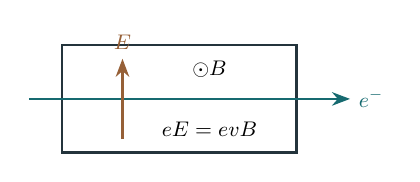
\begin{tikzpicture}[scale=.85,transform shape]

\draw[object] (-.5,-.8) rectangle (3,.8);
\draw[motion] (-1,0)--(3.8,0) node[right] {$e^-$};
\draw[force] (.4,-.6)--(.4,.6) node[above] {$E$};
\node at (1.7,.45) {$\odot B$};
\node at (1.7,-.45) {$eE=evB$};

\end{tikzpicture}
\figcaption{解图综五.2A\quad 交叉场选出速率，再以磁偏转曲率求荷质比；负号由方向判断。}
\end{minipage}\end{center}
\textbf{（1）阴极射线与电子荷质比。}
解图综五.2A中，真空放电产生的阴极射线经过狭缝形成束流。汤姆孙观察其在电场和磁场中的偏转，测出带负电粒子的荷质比，并比较不同气体和电极材料所产生的射线。它们表现出相同类型的带电粒子性质，支持电子是物质中的共同成分。

定量原理可用交叉场和平面磁偏转说明。交叉电场、磁场调到射线不偏时，电力和磁力大小相等，
\[
eE=evB,\qquad v=\frac EB.
\]
再用纯磁场中的曲率半径$r$，有$evB=mv^2/r$，故
\[
\boxed{\frac em=\frac{v}{Br}=\frac{E}{B^2r}}.
\]
这里$e$取电荷量大小，负号由偏转方向判断。测得电子的$e/m$大于氢离子相应值的千倍以上，结合随后基本电荷测量，才可分别确定很小的电子质量。荷质比只给两者的比例，结合基本电荷测量后可由$m=e/(e/m)$得到电子质量。
\begin{center}\begin{minipage}{.98\linewidth}\centering
\begin{tikzpicture}[scale=.85,transform shape]

\draw[object,line width=1.5pt] (-.5,1.1)--(2.8,1.1) (-.5,-1.1)--(2.8,-1.1);
\fill[accent] (1,0) circle (3pt) node[right] {$q$};
\draw[force] (1,0)--(1,.85) node[left] {$qE$};
\draw[force,color=warm] (1,0)--(1,-.85) node[left] {$m_{\rm eff}g$};
\node at (3.5,0) {显微观察};

\end{tikzpicture}
\figcaption{解图综五.2B\quad 重力减浮力由电力平衡；断场终速用来估计油滴尺寸。}
\end{minipage}\end{center}
\textbf{（2）油滴与电荷量子化。}
解图综五.2B的带电小油滴置于两水平极板之间，用显微镜跟踪。先断开电场，油滴向下达到终速$v_f$；重力减浮力与黏滞阻力平衡。在低雷诺数、近似球形的模型下，
\[
\frac43\pi r^3(\rho_{\rm oil}-\rho_{\rm air})g
=6\pi\eta_{\rm air}r v_f.
\]
于是由终速估计油滴半径
\[
r=\sqrt{\frac{9\eta_{\rm air}v_f}
{2(\rho_{\rm oil}-\rho_{\rm air})g}}.
\]
加电场使油滴悬浮，电力平衡有效重力，故
\[
|q|E=\frac43\pi r^3(\rho_{\rm oil}-\rho_{\rm air})g,
\qquad
|q|=\frac{6\pi\eta_{\rm air}r v_f}{E}.
\]
精密处理小油滴还需空气滑移等修正，修正后的阻力关系用于提高半径和电荷读数的准确度。

重复测不同油滴，或观察同一油滴带电量的离散改变，发现电荷量可表成$q=ne$，$n$为整数，进而测定基本电荷$e$。这一结论比“油滴会受电力”多了一层：测量显示电荷改变以共同单位发生。1910年前后的工作通过大量油滴、带电变化及阻力修正逐步提高精度，之后继续改进。
\begin{center}\begin{minipage}{.98\linewidth}\centering
\begin{tikzpicture}[scale=.85,transform shape]

\draw[object,line width=2pt] (.5,-1.2)--(.5,1.2);
\draw[motion] (-2,0)--(.4,0);
\foreach \ang in {-10,0,10,65,140}{\draw[motion] (.5,0)--++(\ang:2);}
\node[below] at (.5,-1.2) {薄箔};
\node[above] at (-1.5,.2) {$\alpha$束};

\end{tikzpicture}
\figcaption{解图综五.2C\quad 同一入射束以小角为主、极少数大角偏转，限制正电荷的空间分布。}
\end{minipage}\end{center}
\textbf{（3）大角散射与原子核。}
解图综五.2C用准直$\alpha$粒子束照射薄金属箔，通过周围可移动探测屏记录散射方向。所述厚约$10^{-6}\,\mathrm m$的薄金箔实验中，多数粒子偏转很小、绝大部分在$1^\circ$以内，约八千分之一的粒子偏转大于$90^\circ$。若正电荷弥散于整个原子，单次作用通常太弱，难以解释这种少量但显著的大角散射。

卢瑟福于1911年据此提出原子的正电荷和大部分质量集中在很小的核内，原子的大部分体积可让高速粒子近乎穿行。对足够薄的靶，以单次散射、重核近似和排斥库仑力为模型，设$\kappa_\alpha=Zze^2/(4\pi\epsilon_0)$，入射动能为$E_\alpha$、碰撞参数为$b$，有
\[
b=\frac{\kappa_\alpha}{2E_\alpha}\cot\frac\theta2,\qquad
\frac{d\sigma}{d\Omega}
=\left(\frac{\kappa_\alpha}{4E_\alpha}\right)^2
\frac1{\sin^4(\theta/2)}.
\]
角分布和能量依赖用于比较小尺度库仑中心模型与测量。实验支持核式结构，电子稳定态和能级还需相应的量子理论描述。
\begin{center}\begin{minipage}{.98\linewidth}\centering
\begin{tikzpicture}[scale=.85,transform shape]

\draw[object] (-1,-.9) rectangle (4,1);
\draw[object,line width=1.4pt] (0,-.6)--(0,.6) (2.5,-.6)--(2.5,.6) (3.5,-.6)--(3.5,.6);
\draw[motion] (.3,0)--(2.2,0);
\node[above] at (.8,1) {汞蒸气};
\node[below] at (1.3,-.9) {加速$U$};
\node[right] at (4.1,.2) {收集};

\end{tikzpicture}
\figcaption{解图综五.2D\quad 加速区、汞蒸气与反向收集区使离散能量损失显示为电流下降。}
\end{minipage}\end{center}
\textbf{（4）非弹性碰撞与离散激发能。}
解图综五.2D中，电子被加速电压$U$加速，穿过汞蒸气，再克服一个小反向电势到达收集极。随着$U$增大，收集电流随电压总体上升，并在近似等间距电压处反复出现下降。

在汞的典型实验条件下，间距约$4.9\,\mathrm V$。当电子获得足够动能，可通过非弹性碰撞把约$4.9\,\mathrm{eV}$交给一个汞原子，自己损失这部分能量，因而有些电子在反向场中折返，收集电流随之下降。电压再提高，电子可在到达前发生两次、三次这样的能量损失，于是形成重复结构。
\[
\Delta E=e\,\Delta U,\qquad
\Delta U\simeq4.9\,\mathrm V.
\]
这说明原子吸收的激发能不是任意连续值，而有确定的能级差。若将该能量以一个光子释放，波长约为
$hc/\Delta E\simeq253\,\mathrm{nm}$。电流峰谷的绝对位置还受接触电势、温度和碰撞位置影响；相邻间距比单个峰位置更直接反映激发能。这一结果与玻尔模型中离散定态的核心假设相符，实验直接测得的是确定的激发能差。
\begin{center}\begin{minipage}{.98\linewidth}\centering
\begin{tikzpicture}[scale=.85,transform shape]

\fill (0,0) circle (2pt) node[left] {$\odot$扭轴};
\draw[object] (0,0)--(2,0);
\draw[object,line width=2pt] (1.6,0)--(2.4,0);
\draw[motion] (1.8,-1)--(1.8,-.1);
\draw[motion] (2.1,-1)--(2.1,-.1);
\draw[force] (2,.1)--(2,1.4) node[right] {$F$};
\draw[guide] (.6,0) arc[start angle=0,end angle=40,radius=.6];
\node at (.8,.6) {扭角};
\node at (1,-1.4) {俯视：光束沿纸面入射};

\end{tikzpicture}
\figcaption{解图综五.2E\quad 辐射给薄片动量，扭丝回复力矩平衡微小光压。}
\end{minipage}\end{center}
\textbf{（5）光压与辐射动量。}
解图综五.2E把薄片悬在灵敏扭秤上，光照后由扭转角估计作用力。列别捷夫与尼科尔斯、赫尔的研究测量了很小的辐射压力，并处理热效应、残余气体等影响，确认光可以向物体传递动量。

若光束以强度$I$正入射，完全吸收时每单位时间、单位面积传递能量$I$及动量$I/c$，压力为
\[
p_{\rm abs}=\frac Ic.
\]
完全镜面反射使法向动量反向，改变为两倍，故$p_{\rm refl}=2I/c$。受照面积$A$对应力$F=pA$，扭矩再与扭秤回复力矩平衡。这是光携带动量的直接测量，经典电磁理论和光子描述均给出光压；康普顿散射中的角度依赖波长位移进一步呈现单次光子碰撞的关系。
\begin{center}\begin{minipage}{.98\linewidth}\centering
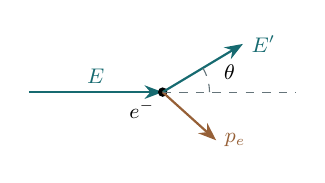
\begin{tikzpicture}[scale=.85,transform shape]

\draw[motion] (-2,0)--(0,0) node[midway,above] {$E$};
\fill (0,0) circle (2pt) node[below left] {$e^-$};
\draw[motion] (0,0)--(1.2,.72) node[right] {$E'$};
\draw[force] (0,0)--(.8,-.72) node[right] {$p_e$};
\draw[guide] (0,0)--(2,0);
\draw[guide] (.7,0) arc[start angle=0,end angle=30.96,radius=.7];
\node at (1,.3) {$\theta$};

\end{tikzpicture}
\figcaption{解图综五.2F\quad 光子散射方向与电子反冲共同满足能量动量守恒。}
\end{minipage}\end{center}
\textbf{（6）康普顿波长位移。}
解图综五.2F中，以X射线照射石墨等物质并测不同散射角$\theta$的光谱。散射谱中出现比入射波长更长的分量，其位移随角度变化。用光子与近似自由、起初静止电子碰撞，可由能量和动量守恒解释。

设入射、散射光子能量分别为$E,E'$，电子反冲动量为$\boldsymbol p_e$。守恒式为
\[
E+m_ec^2=E'+\sqrt{m_e^2c^4+p_e^2c^2},
\quad
\boldsymbol p_e=\frac Ec\hat{\boldsymbol n}
-\frac{E'}c\hat{\boldsymbol n}'.
\]
动量式平方给$p_e^2c^2=E^2+E'^2-2EE'\cos\theta$；能量式移项平方则给
$p_e^2c^2=(E-E')^2+2m_ec^2(E-E')$。相减得到
\[
EE'(1-\cos\theta)=m_ec^2(E-E').
\]
再用$E=hc/\lambda,E'=hc/\lambda'$，
\[
\boxed{\lambda'-\lambda=\frac{h}{m_ec}(1-\cos\theta)}.
\]
该角度规律不取决于照射强度，支持光子的能量—动量描述。近自由、初始静止电子是此式的条件；束缚电子或整体物体的散射可产生不同分量，谱中各分量需按相应反冲模型解释。
\begin{center}\begin{minipage}{.98\linewidth}\centering
\begin{tikzpicture}[scale=.85,transform shape]

\foreach \y in {0,-.5,-1}{\draw[object] (-2,\y)--(2,\y);}
\draw[motion] (-2,1.3)--(0,0);
\draw[motion] (0,0)--(2,1.3) node[right] {峰方向};
\draw[guide] (.8,0) arc[start angle=0,end angle=33,radius=.8];
\node at (1.2,.3) {$\theta_B$};
\node[left] at (-2,-.25) {$d$};

\end{tikzpicture}
\figcaption{解图综五.2G\quad 布拉格角相对晶面定义，峰位置须和实际探测角换算。}
\end{minipage}\end{center}
\textbf{（7）晶体电子衍射与物质波。}
解图综五.2G中，具有已知加速能量的电子束照射镍单晶，探测器测电子强度随方向的变化。某些方向出现显著峰值，并随电子能量和晶体方向改变，与波的相干衍射相符。

电子加速电压为$U$，在非相对论范围内$p=\sqrt{2m_eeU}$，德布罗意波长
\[
\lambda=\frac hp=\frac{h}{\sqrt{2m_eeU}}.
\]
晶面间距$d$已知时，布拉格干涉条件为$2d\sin\theta_B=n\lambda$，其中$\theta_B$是束流与晶面的掠射角，探测器报告角依其入射、出射方向定义换算后使用。由角分布反推的波长与$h/p$一致，证实电子的波动性。例如$U=54\,\mathrm V$给$\lambda\simeq0.167\,\mathrm{nm}$，与晶体原子尺度相当，所以可见明显衍射。
\begin{center}\begin{minipage}{.98\linewidth}\centering
\begin{tikzpicture}[scale=.85,transform shape]

\coordinate (O) at (0,0);
\draw[object] (-1,0)--(2,0) (0,-1)--(0,2);
\draw[object,line width=2pt] (2,-.4)--(2,.4) (-.4,2)--(.4,2);
\draw[object,line width=1.3pt] (-.4,-.4)--(.4,.4);
\draw[motion] (-1,0)--(-.5,0);
\draw[motion] (.4,.15)--(1.7,.15);
\draw[motion] (.15,.4)--(.15,1.7);
\node[below] at (1,0) {$L$};\node[left] at (0,1) {$L$};
\node at (2,-1) {转90度比较条纹};

\end{tikzpicture}
\figcaption{解图综五.2H\quad 等长正交臂分束后重新干涉，转动装置比较方向相关的往返时间差。}
\end{minipage}\end{center}
\textbf{（8）正交光臂与以太风预言。}
解图综五.2H将同一光束分到两条正交光臂，反射后重合干涉，并将装置转动以比较条纹。1887年的合作实验在1881年先前尝试的基础上提高了灵敏度。

在作为比较对象的简单静止以太模型中，若装置相对以太以$v$运动，取两臂单程等效长度均为$L$、以太中光速$c$，平行臂往返时间为
\[
t_\parallel=\frac L{c-v}+\frac L{c+v}
=\frac{2Lc}{c^2-v^2}.
\]
垂直臂要随装置横移，往返时间为
$t_\perp=2L/\sqrt{c^2-v^2}$。在$v\ll c$下，
\[
t_\parallel-t_\perp\simeq\frac{Lv^2}{c^3}.
\]
装置转$90^\circ$使两臂交换角色，预期时间差改变两倍，对应条纹移动数
\[
\Delta n\simeq\frac{2Lv^2}{\lambda c^2}.
\]
实际未发现与该预期相符的明显周期性移动。这一零结果约束了上述简单以太风模型，是后来相对论发展的实验背景之一。狭义相对论以真空光速与惯性系规律的一致性解释它；该实验直接比较的是光的往返传播，相对性原理涉及更广的物理规律和实验事实；不同介质假设则按各自的传播预言与实验比较。


\Needspace{8\baselineskip}

\pdfbookmark[3]{关键洞察}{q2-h5}

\subsection*{关键洞察}

\begin{itemize}
\item 光压显示光传递动量，经典电磁理论与光子理论均给出这一效应；康普顿的角度依赖波长变化进一步呈现单次碰撞的能量动量关系。
\item 油滴电荷测量依赖尺寸、空气阻力和电场，电子衍射依赖晶面间距与角度。把这些量连成测量关系，实验结论才有可计算内容。
\item 条纹零结果对应明确的预言及灵敏度。将平行、垂直臂的往返时间算出，再比较旋转前后，能够说明受约束的是哪一类传播模型。
\end{itemize}

\Needspace{8\baselineskip}

\pdfbookmark[3]{易错点}{q2-h6}

\subsection*{易错点}

\begin{itemize}
\item 把荷质比当作两个独立测量量，或把每滴油都当作只带一个基本电荷，会丢失两个实验互补的作用。
\item 约4.9伏的相邻结构反映汞原子的离散激发能；电离需另一个更高的能量。绝对峰位还受接触电势及碰撞分布影响。
\item 光压中的光强、康普顿式中的光子能量、衍射中的电子加速电压和晶面角分别控制不同读数。将同一“能量”或“散射角”名称直接代入，容易错置物理量。
\item 迈克耳孙的早期尝试和与莫雷的合作实验有不同年份。该干涉实验直接比较光的往返传播；相对性原理涉及更广的物理规律与实验事实。
\end{itemize}

\Needspace{8\baselineskip}

\pdfbookmark[3]{课堂讲解建议}{q2-h7}

\subsection*{课堂讲解建议}

\begin{itemize}
\item 请学生为每个图写三句话：改变哪个量、记录哪个量、利用什么关系计算。随后由这些读数说出实验支持的结论，使回答包含完整测量过程。
\item 将图A、B连起来，问测得$e/m$后还缺什么才能得到电子质量。答还需基本电荷$e$的测量，再用$m=e/(e/m)$说明两类实验如何互补，并讨论油滴电荷呈整数倍这一实际观察。
\item 并列比较光压、光电效应、康普顿和电子衍射，分别用动量通量、能量阈值、波长位移及物质波干涉解释读数。每个“波”或“粒子”结论都落在一个具体关系上。
\item 用给定$L/\lambda$与$v/c$算预期条纹数，再与能分辨的最小条纹变化比较。追问没有观察到预期移动时可得到什么结论。答在装置足以分辨该条纹量级时，测量限制了这一简单静止以太模型的传播预言；随后讨论光的往返测量与一般相对性原理各自涉及的物理内容。
\end{itemize}

\Needspace{8\baselineskip}

\pdfbookmark[3]{变式训练}{q2-h8}

\subsection*{变式训练}

\begin{enumerate}
\Needspace{37\baselineskip}
\item \textbf{题设与求解。} 交叉场$E,B$和纯磁偏转半径$r$给$e/m=E/(B^2r)$。对小相对误差取对数微分，
\[
\frac{\delta(e/m)}{e/m}
=\frac{\delta E}{E}-2\frac{\delta B}{B}-\frac{\delta r}{r}.
\]
仅$r$偏大$1\%$时，读数精确变为$1/1.01$倍，约偏小$1\%$；仅$B$偏大$1\%$时，变为$1/(1.01)^2$倍，约偏小$2\%$。图V1画两个单独偏差的响应，磁场误差在一阶有两倍权重。
\begin{center}\begin{minipage}{.98\linewidth}\centering
\begin{tikzpicture}[scale=0.72,transform shape]
\draw[axis] (0,0)--(6.2,0);\draw[axis] (0,0)--(0,3.4000000000000004);
\draw[thin,color=muted] (0.0000000,0)--(0.0000000,-.07);\node[below] at (0.0000000,-.09) {$-.04$};
\draw[thin,color=muted] (3.0000000,0)--(3.0000000,-.07);\node[below] at (3.0000000,-.09) {$0$};
\draw[thin,color=muted] (6.0000000,0)--(6.0000000,-.07);\node[below] at (6.0000000,-.09) {$.04$};
\draw[thin,color=muted] (0,0.3764706)--(-.07,0.3764706);\node[left] at (-.09,0.3764706) {$.94$};
\draw[thin,color=muted] (0,1.5058824)--(-.07,1.5058824);\node[left] at (-.09,1.5058824) {$1$};
\draw[thin,color=muted] (0,3.0117647)--(-.07,3.0117647);\node[left] at (-.09,3.0117647) {$1.08$};
\node[below] at (3.0,-.64) {单项读数相对偏差};\node[above right] at (0,3.45) {推得的$(e/m)$除以正确值};
\draw[traj] plot coordinates {(0.0000000,2.2901961) (0.0250000,2.2833902) (0.0500000,2.2765890) (0.0750000,2.2697925) (0.1000000,2.2630007) (0.1250000,2.2562137) (0.1500000,2.2494313) (0.1750000,2.2426537) (0.2000000,2.2358807) (0.2250000,2.2291125) (0.2500000,2.2223489) (0.2750000,2.2155900) (0.3000000,2.2088357) (0.3250000,2.2020862) (0.3500000,2.1953413) (0.3750000,2.1886010) (0.4000000,2.1818655) (0.4250000,2.1751345) (0.4500000,2.1684082) (0.4750000,2.1616866) (0.5000000,2.1549696) (0.5250000,2.1482572) (0.5500000,2.1415494) (0.5750000,2.1348463) (0.6000000,2.1281478) (0.6250000,2.1214539) (0.6500000,2.1147646) (0.6750000,2.1080799) (0.7000000,2.1013998) (0.7250000,2.0947243) (0.7500000,2.0880534) (0.7750000,2.0813870) (0.8000000,2.0747253) (0.8250000,2.0680681) (0.8500000,2.0614155) (0.8750000,2.0547674) (0.9000000,2.0481239) (0.9250000,2.0414850) (0.9500000,2.0348506) (0.9750000,2.0282208) (1.0000000,2.0215955) (1.0250000,2.0149747) (1.0500000,2.0083585) (1.0750000,2.0017468) (1.1000000,1.9951396) (1.1250000,1.9885370) (1.1500000,1.9819388) (1.1750000,1.9753452) (1.2000000,1.9687560) (1.2250000,1.9621714) (1.2500000,1.9555912) (1.2750000,1.9490156) (1.3000000,1.9424444) (1.3250000,1.9358777) (1.3500000,1.9293155) (1.3750000,1.9227578) (1.4000000,1.9162045) (1.4250000,1.9096557) (1.4500000,1.9031114) (1.4750000,1.8965715) (1.5000000,1.8900360) (1.5250000,1.8835050) (1.5500000,1.8769784) (1.5750000,1.8704563) (1.6000000,1.8639386) (1.6250000,1.8574253) (1.6500000,1.8509165) (1.6750000,1.8444121) (1.7000000,1.8379120) (1.7250000,1.8314164) (1.7500000,1.8249252) (1.7750000,1.8184384) (1.8000000,1.8119560) (1.8250000,1.8054780) (1.8500000,1.7990043) (1.8750000,1.7925351) (1.9000000,1.7860702) (1.9250000,1.7796097) (1.9500000,1.7731536) (1.9750000,1.7667018) (2.0000000,1.7602544) (2.0250000,1.7538113) (2.0500000,1.7473726) (2.0750000,1.7409382) (2.1000000,1.7345082) (2.1250000,1.7280825) (2.1500000,1.7216612) (2.1750000,1.7152442) (2.2000000,1.7088315) (2.2250000,1.7024231) (2.2500000,1.6960190) (2.2750000,1.6896193) (2.3000000,1.6832238) (2.3250000,1.6768327) (2.3500000,1.6704458) (2.3750000,1.6640633) (2.4000000,1.6576850) (2.4250000,1.6513110) (2.4500000,1.6449413) (2.4750000,1.6385759) (2.5000000,1.6322148) (2.5250000,1.6258579) (2.5500000,1.6195053) (2.5750000,1.6131569) (2.6000000,1.6068128) (2.6250000,1.6004730) (2.6500000,1.5941373) (2.6750000,1.5878060) (2.7000000,1.5814789) (2.7250000,1.5751560) (2.7500000,1.5688373) (2.7750000,1.5625229) (2.8000000,1.5562126) (2.8250000,1.5499066) (2.8500000,1.5436049) (2.8750000,1.5373073) (2.9000000,1.5310139) (2.9250000,1.5247247) (2.9500000,1.5184397) (2.9750000,1.5121590) (3.0000000,1.5058824) (3.0250000,1.4996099) (3.0500000,1.4933417) (3.0750000,1.4870776) (3.1000000,1.4808177) (3.1250000,1.4745620) (3.1500000,1.4683104) (3.1750000,1.4620630) (3.2000000,1.4558198) (3.2250000,1.4495807) (3.2500000,1.4433457) (3.2750000,1.4371149) (3.3000000,1.4308882) (3.3250000,1.4246657) (3.3500000,1.4184472) (3.3750000,1.4122330) (3.4000000,1.4060228) (3.4250000,1.3998167) (3.4500000,1.3936148) (3.4750000,1.3874169) (3.5000000,1.3812232) (3.5250000,1.3750336) (3.5500000,1.3688481) (3.5750000,1.3626666) (3.6000000,1.3564893) (3.6250000,1.3503160) (3.6500000,1.3441468) (3.6750000,1.3379817) (3.7000000,1.3318207) (3.7250000,1.3256637) (3.7500000,1.3195108) (3.7750000,1.3133619) (3.8000000,1.3072171) (3.8250000,1.3010764) (3.8500000,1.2949397) (3.8750000,1.2888071) (3.9000000,1.2826784) (3.9250000,1.2765539) (3.9500000,1.2704333) (3.9750000,1.2643168) (4.0000000,1.2582043) (4.0250000,1.2520959) (4.0500000,1.2459914) (4.0750000,1.2398910) (4.1000000,1.2337945) (4.1250000,1.2277021) (4.1500000,1.2216137) (4.1750000,1.2155293) (4.2000000,1.2094488) (4.2250000,1.2033724) (4.2500000,1.1972999) (4.2750000,1.1912314) (4.3000000,1.1851669) (4.3250000,1.1791064) (4.3500000,1.1730498) (4.3750000,1.1669972) (4.4000000,1.1609486) (4.4250000,1.1549039) (4.4500000,1.1488632) (4.4750000,1.1428264) (4.5000000,1.1367935) (4.5250000,1.1307646) (4.5500000,1.1247397) (4.5750000,1.1187187) (4.6000000,1.1127016) (4.6250000,1.1066884) (4.6500000,1.1006792) (4.6750000,1.0946739) (4.7000000,1.0886724) (4.7250000,1.0826749) (4.7500000,1.0766814) (4.7750000,1.0706917) (4.8000000,1.0647059) (4.8250000,1.0587240) (4.8500000,1.0527460) (4.8750000,1.0467719) (4.9000000,1.0408017) (4.9250000,1.0348353) (4.9500000,1.0288728) (4.9750000,1.0229142) (5.0000000,1.0169595) (5.0250000,1.0110086) (5.0500000,1.0050616) (5.0750000,0.9991185) (5.1000000,0.9931792) (5.1250000,0.9872438) (5.1500000,0.9813122) (5.1750000,0.9753844) (5.2000000,0.9694605) (5.2250000,0.9635405) (5.2500000,0.9576242) (5.2750000,0.9517118) (5.3000000,0.9458032) (5.3250000,0.9398984) (5.3500000,0.9339975) (5.3750000,0.9281004) (5.4000000,0.9222070) (5.4250000,0.9163175) (5.4500000,0.9104318) (5.4750000,0.9045499) (5.5000000,0.8986717) (5.5250000,0.8927974) (5.5500000,0.8869268) (5.5750000,0.8810601) (5.6000000,0.8751971) (5.6250000,0.8693379) (5.6500000,0.8634824) (5.6750000,0.8576308) (5.7000000,0.8517829) (5.7250000,0.8459387) (5.7500000,0.8400984) (5.7750000,0.8342617) (5.8000000,0.8284289) (5.8250000,0.8225997) (5.8500000,0.8167743) (5.8750000,0.8109527) (5.9000000,0.8051348) (5.9250000,0.7993206) (5.9500000,0.7935102) (5.9750000,0.7877034) (6.0000000,0.7819005)};
\draw[traj] (.1,-1.05)--(.7,-1.05);\node[right] at (.85,-1.05) {仅半径读数有偏差};\draw[dashed,thick,color=warm] plot coordinates {(0.0000000,3.1071895) (0.0250000,3.0930130) (0.0500000,3.0788512) (0.0750000,3.0647042) (0.1000000,3.0505719) (0.1250000,3.0364542) (0.1500000,3.0223513) (0.1750000,3.0082630) (0.2000000,2.9941893) (0.2250000,2.9801302) (0.2500000,2.9660857) (0.2750000,2.9520558) (0.3000000,2.9380405) (0.3250000,2.9240397) (0.3500000,2.9100534) (0.3750000,2.8960815) (0.4000000,2.8821242) (0.4250000,2.8681813) (0.4500000,2.8542528) (0.4750000,2.8403388) (0.5000000,2.8264391) (0.5250000,2.8125538) (0.5500000,2.7986829) (0.5750000,2.7848263) (0.6000000,2.7709840) (0.6250000,2.7571560) (0.6500000,2.7433422) (0.6750000,2.7295428) (0.7000000,2.7157575) (0.7250000,2.7019865) (0.7500000,2.6882297) (0.7750000,2.6744870) (0.8000000,2.6607585) (0.8250000,2.6470441) (0.8500000,2.6333439) (0.8750000,2.6196577) (0.9000000,2.6059857) (0.9250000,2.5923276) (0.9500000,2.5786837) (0.9750000,2.5650537) (1.0000000,2.5514377) (1.0250000,2.5378358) (1.0500000,2.5242478) (1.0750000,2.5106737) (1.1000000,2.4971136) (1.1250000,2.4835673) (1.1500000,2.4700350) (1.1750000,2.4565165) (1.2000000,2.4430118) (1.2250000,2.4295210) (1.2500000,2.4160440) (1.2750000,2.4025808) (1.3000000,2.3891314) (1.3250000,2.3756957) (1.3500000,2.3622738) (1.3750000,2.3488656) (1.4000000,2.3354710) (1.4250000,2.3220902) (1.4500000,2.3087230) (1.4750000,2.2953695) (1.5000000,2.2820295) (1.5250000,2.2687032) (1.5500000,2.2553905) (1.5750000,2.2420913) (1.6000000,2.2288057) (1.6250000,2.2155337) (1.6500000,2.2022751) (1.6750000,2.1890300) (1.7000000,2.1757984) (1.7250000,2.1625803) (1.7500000,2.1493756) (1.7750000,2.1361843) (1.8000000,2.1230065) (1.8250000,2.1098420) (1.8500000,2.0966909) (1.8750000,2.0835531) (1.9000000,2.0704286) (1.9250000,2.0573175) (1.9500000,2.0442197) (1.9750000,2.0311351) (2.0000000,2.0180639) (2.0250000,2.0050058) (2.0500000,1.9919610) (2.0750000,1.9789293) (2.1000000,1.9659109) (2.1250000,1.9529056) (2.1500000,1.9399135) (2.1750000,1.9269346) (2.2000000,1.9139687) (2.2250000,1.9010159) (2.2500000,1.8880762) (2.2750000,1.8751496) (2.3000000,1.8622361) (2.3250000,1.8493355) (2.3500000,1.8364480) (2.3750000,1.8235734) (2.4000000,1.8107119) (2.4250000,1.7978633) (2.4500000,1.7850276) (2.4750000,1.7722049) (2.5000000,1.7593950) (2.5250000,1.7465981) (2.5500000,1.7338140) (2.5750000,1.7210428) (2.6000000,1.7082844) (2.6250000,1.6955389) (2.6500000,1.6828061) (2.6750000,1.6700862) (2.7000000,1.6573790) (2.7250000,1.6446845) (2.7500000,1.6320028) (2.7750000,1.6193338) (2.8000000,1.6066775) (2.8250000,1.5940339) (2.8500000,1.5814030) (2.8750000,1.5687847) (2.9000000,1.5561790) (2.9250000,1.5435860) (2.9500000,1.5310055) (2.9750000,1.5184376) (3.0000000,1.5058824) (3.0250000,1.4933396) (3.0500000,1.4808094) (3.0750000,1.4682917) (3.1000000,1.4557865) (3.1250000,1.4432938) (3.1500000,1.4308135) (3.1750000,1.4183457) (3.2000000,1.4058903) (3.2250000,1.3934474) (3.2500000,1.3810168) (3.2750000,1.3685987) (3.3000000,1.3561929) (3.3250000,1.3437994) (3.3500000,1.3314183) (3.3750000,1.3190495) (3.4000000,1.3066930) (3.4250000,1.2943487) (3.4500000,1.2820168) (3.4750000,1.2696971) (3.5000000,1.2573896) (3.5250000,1.2450944) (3.5500000,1.2328114) (3.5750000,1.2205405) (3.6000000,1.2082818) (3.6250000,1.1960353) (3.6500000,1.1838009) (3.6750000,1.1715787) (3.7000000,1.1593685) (3.7250000,1.1471704) (3.7500000,1.1349845) (3.7750000,1.1228105) (3.8000000,1.1106486) (3.8250000,1.0984988) (3.8500000,1.0863609) (3.8750000,1.0742351) (3.9000000,1.0621212) (3.9250000,1.0500193) (3.9500000,1.0379294) (3.9750000,1.0258513) (4.0000000,1.0137852) (4.0250000,1.0017310) (4.0500000,0.9896887) (4.0750000,0.9776583) (4.1000000,0.9656397) (4.1250000,0.9536329) (4.1500000,0.9416380) (4.1750000,0.9296549) (4.2000000,0.9176835) (4.2250000,0.9057240) (4.2500000,0.8937762) (4.2750000,0.8818401) (4.3000000,0.8699158) (4.3250000,0.8580032) (4.3500000,0.8461023) (4.3750000,0.8342131) (4.4000000,0.8223356) (4.4250000,0.8104697) (4.4500000,0.7986154) (4.4750000,0.7867728) (4.5000000,0.7749418) (4.5250000,0.7631223) (4.5500000,0.7513145) (4.5750000,0.7395182) (4.6000000,0.7277335) (4.6250000,0.7159603) (4.6500000,0.7041986) (4.6750000,0.6924484) (4.7000000,0.6807097) (4.7250000,0.6689825) (4.7500000,0.6572667) (4.7750000,0.6455624) (4.8000000,0.6338695) (4.8250000,0.6221880) (4.8500000,0.6105179) (4.8750000,0.5988592) (4.9000000,0.5872119) (4.9250000,0.5755759) (4.9500000,0.5639513) (4.9750000,0.5523380) (5.0000000,0.5407360) (5.0250000,0.5291453) (5.0500000,0.5175658) (5.0750000,0.5059977) (5.1000000,0.4944408) (5.1250000,0.4828951) (5.1500000,0.4713606) (5.1750000,0.4598374) (5.2000000,0.4483253) (5.2250000,0.4368245) (5.2500000,0.4253348) (5.2750000,0.4138562) (5.3000000,0.4023888) (5.3250000,0.3909325) (5.3500000,0.3794873) (5.3750000,0.3680532) (5.4000000,0.3566302) (5.4250000,0.3452182) (5.4500000,0.3338173) (5.4750000,0.3224274) (5.5000000,0.3110485) (5.5250000,0.2996807) (5.5500000,0.2883238) (5.5750000,0.2769779) (5.6000000,0.2656430) (5.6250000,0.2543191) (5.6500000,0.2430060) (5.6750000,0.2317039) (5.7000000,0.2204127) (5.7250000,0.2091324) (5.7500000,0.1978630) (5.7750000,0.1866044) (5.8000000,0.1753567) (5.8250000,0.1641198) (5.8500000,0.1528938) (5.8750000,0.1416785) (5.9000000,0.1304741) (5.9250000,0.1192804) (5.9500000,0.1080975) (5.9750000,0.0969254) (6.0000000,0.0857640)};
\draw[dashed,thick,color=warm] (.1,-1.48)--(.7,-1.48);\node[right] at (.85,-1.48) {仅磁场读数有偏差};\end{tikzpicture}
\figcaption{解图综五.2V1\quad 磁场平方进入测量式，小偏差的一阶权重为2}
\end{minipage}\end{center}
\Needspace{37\baselineskip}
\item \textbf{题设与求解。} 汞的激发能取$4.9\,\mathrm{eV}$，原子以一个光子释放这一能量，求波长。由$hc\simeq1240\,\mathrm{eV\,nm}$，有$\lambda=hc/\Delta E\simeq253.1\,\mathrm{nm}$。图V2画能级差与发射波长的反比关系，4.9电子伏对应紫外光。碰撞先把电子动能交给原子，去激发才将能量释放；实际探测到的光子数还受去激发过程及探测效率影响。
\begin{center}\begin{minipage}{.98\linewidth}\centering
\begin{tikzpicture}[scale=0.72,transform shape]
\draw[axis] (0,0)--(6.2,0);\draw[axis] (0,0)--(0,3.4000000000000004);
\draw[thin,color=muted] (0.0000000,0)--(0.0000000,-.07);\node[below] at (0.0000000,-.09) {$2$};
\draw[thin,color=muted] (2.9000000,0)--(2.9000000,-.07);\node[below] at (2.9000000,-.09) {$4.9$};
\draw[thin,color=muted] (6.0000000,0)--(6.0000000,-.07);\node[below] at (6.0000000,-.09) {$8$};
\draw[thin,color=muted] (0,0.3764706)--(-.07,0.3764706);\node[left] at (-.09,0.3764706) {$200$};
\draw[thin,color=muted] (0,0.7094036)--(-.07,0.7094036);\node[left] at (-.09,0.7094036) {$253$};
\draw[thin,color=muted] (0,2.8862745)--(-.07,2.8862745);\node[left] at (-.09,2.8862745) {$600$};
\node[below] at (3.0,-.64) {能级差（eV）};\node[above right] at (0,3.45) {波长（nm）};
\draw[traj] plot coordinates {(0.0000000,3.0117647) (0.0250000,2.9637376) (0.0500000,2.9168819) (0.0750000,2.8711552) (0.1000000,2.8265173) (0.1250000,2.7829296) (0.1500000,2.7403557) (0.1750000,2.6987604) (0.2000000,2.6581105) (0.2250000,2.6183741) (0.2500000,2.5795207) (0.2750000,2.5415212) (0.3000000,2.5043478) (0.3250000,2.4679739) (0.3500000,2.4323738) (0.3750000,2.3975232) (0.4000000,2.3633987) (0.4250000,2.3299778) (0.4500000,2.2972389) (0.4750000,2.2651614) (0.5000000,2.2337255) (0.5250000,2.2029121) (0.5500000,2.1727028) (0.5750000,2.1430801) (0.6000000,2.1140271) (0.6250000,2.0855275) (0.6500000,2.0575657) (0.6750000,2.0301264) (0.7000000,2.0031954) (0.7250000,1.9767584) (0.7500000,1.9508021) (0.7750000,1.9253135) (0.8000000,1.9002801) (0.8250000,1.8756897) (0.8500000,1.8515308) (0.8750000,1.8277920) (0.9000000,1.8044625) (0.9250000,1.7815318) (0.9500000,1.7589897) (0.9750000,1.7368265) (1.0000000,1.7150327) (1.0250000,1.6935991) (1.0500000,1.6725169) (1.0750000,1.6517775) (1.1000000,1.6313725) (1.1250000,1.6112941) (1.1500000,1.5915344) (1.1750000,1.5720858) (1.2000000,1.5529412) (1.2250000,1.5340933) (1.2500000,1.5155354) (1.2750000,1.4972609) (1.3000000,1.4792632) (1.3250000,1.4615362) (1.3500000,1.4440737) (1.3750000,1.4268700) (1.4000000,1.4099193) (1.4250000,1.3932160) (1.4500000,1.3767548) (1.4750000,1.3605304) (1.5000000,1.3445378) (1.5250000,1.3287721) (1.5500000,1.3132284) (1.5750000,1.2979021) (1.6000000,1.2827887) (1.6250000,1.2678837) (1.6500000,1.2531829) (1.6750000,1.2386821) (1.7000000,1.2243773) (1.7250000,1.2102645) (1.7500000,1.1963399) (1.7750000,1.1825997) (1.8000000,1.1690402) (1.8250000,1.1556581) (1.8500000,1.1424497) (1.8750000,1.1294118) (1.9000000,1.1165410) (1.9250000,1.1038341) (1.9500000,1.0912882) (1.9750000,1.0789000) (2.0000000,1.0666667) (2.0250000,1.0545853) (2.0500000,1.0426531) (2.0750000,1.0308673) (2.1000000,1.0192253) (2.1250000,1.0077243) (2.1500000,0.9963619) (2.1750000,0.9851356) (2.2000000,0.9740430) (2.2250000,0.9630816) (2.2500000,0.9522491) (2.2750000,0.9415434) (2.3000000,0.9309622) (2.3250000,0.9205032) (2.3500000,0.9101645) (2.3750000,0.8999440) (2.4000000,0.8898396) (2.4250000,0.8798493) (2.4500000,0.8699714) (2.4750000,0.8602037) (2.5000000,0.8505447) (2.5250000,0.8409923) (2.5500000,0.8315449) (2.5750000,0.8222008) (2.6000000,0.8129582) (2.6250000,0.8038156) (2.6500000,0.7947712) (2.6750000,0.7858236) (2.7000000,0.7769712) (2.7250000,0.7682125) (2.7500000,0.7595459) (2.7750000,0.7509701) (2.8000000,0.7424837) (2.8250000,0.7340851) (2.8500000,0.7257732) (2.8750000,0.7175465) (2.9000000,0.7094038) (2.9250000,0.7013437) (2.9500000,0.6933650) (2.9750000,0.6854665) (3.0000000,0.6776471) (3.0250000,0.6699054) (3.0500000,0.6622403) (3.0750000,0.6546508) (3.1000000,0.6471357) (3.1250000,0.6396939) (3.1500000,0.6323244) (3.1750000,0.6250260) (3.2000000,0.6177979) (3.2250000,0.6106389) (3.2500000,0.6035481) (3.2750000,0.5965245) (3.3000000,0.5895671) (3.3250000,0.5826751) (3.3500000,0.5758475) (3.3750000,0.5690834) (3.4000000,0.5623820) (3.4250000,0.5557423) (3.4500000,0.5491635) (3.4750000,0.5426448) (3.5000000,0.5361854) (3.5250000,0.5297844) (3.5500000,0.5234411) (3.5750000,0.5171547) (3.6000000,0.5109244) (3.6250000,0.5047495) (3.6500000,0.4986292) (3.6750000,0.4925628) (3.7000000,0.4865497) (3.7250000,0.4805891) (3.7500000,0.4746803) (3.7750000,0.4688227) (3.8000000,0.4630156) (3.8250000,0.4572583) (3.8500000,0.4515502) (3.8750000,0.4458907) (3.9000000,0.4402792) (3.9250000,0.4347150) (3.9500000,0.4291976) (3.9750000,0.4237263) (4.0000000,0.4183007) (4.0250000,0.4129200) (4.0500000,0.4075839) (4.0750000,0.4022916) (4.1000000,0.3970428) (4.1250000,0.3918367) (4.1500000,0.3866730) (4.1750000,0.3815512) (4.2000000,0.3764706) (4.2250000,0.3714308) (4.2500000,0.3664314) (4.2750000,0.3614718) (4.3000000,0.3565515) (4.3250000,0.3516702) (4.3500000,0.3468272) (4.3750000,0.3420223) (4.4000000,0.3372549) (4.4250000,0.3325246) (4.4500000,0.3278310) (4.4750000,0.3231736) (4.5000000,0.3185520) (4.5250000,0.3139659) (4.5500000,0.3094148) (4.5750000,0.3048982) (4.6000000,0.3004159) (4.6250000,0.2959674) (4.6500000,0.2915524) (4.6750000,0.2871704) (4.7000000,0.2828212) (4.7250000,0.2785043) (4.7500000,0.2742193) (4.7750000,0.2699660) (4.8000000,0.2657439) (4.8250000,0.2615528) (4.8500000,0.2573923) (4.8750000,0.2532620) (4.9000000,0.2491617) (4.9250000,0.2450910) (4.9500000,0.2410495) (4.9750000,0.2370370) (5.0000000,0.2330532) (5.0250000,0.2290978) (5.0500000,0.2251704) (5.0750000,0.2212707) (5.1000000,0.2173985) (5.1250000,0.2135535) (5.1500000,0.2097354) (5.1750000,0.2059438) (5.2000000,0.2021786) (5.2250000,0.1984395) (5.2500000,0.1947262) (5.2750000,0.1910383) (5.3000000,0.1873758) (5.3250000,0.1837382) (5.3500000,0.1801254) (5.3750000,0.1765371) (5.4000000,0.1729730) (5.4250000,0.1694329) (5.4500000,0.1659166) (5.4750000,0.1624238) (5.5000000,0.1589542) (5.5250000,0.1555078) (5.5500000,0.1520841) (5.5750000,0.1486831) (5.6000000,0.1453044) (5.6250000,0.1419479) (5.6500000,0.1386134) (5.6750000,0.1353005) (5.7000000,0.1320092) (5.7250000,0.1287391) (5.7500000,0.1254902) (5.7750000,0.1222622) (5.8000000,0.1190548) (5.8250000,0.1158679) (5.8500000,0.1127014) (5.8750000,0.1095549) (5.9000000,0.1064284) (5.9250000,0.1033216) (5.9500000,0.1002343) (5.9750000,0.0971664) (6.0000000,0.0941176)};
\draw[traj] (.1,-1.05)--(.7,-1.05);\node[right] at (.85,-1.05) {单光子释放对应的波长};\end{tikzpicture}
\figcaption{解图综五.2V2\quad 汞的约4.9电子伏激发对应约253纳米紫外波长}
\end{minipage}\end{center}
\Needspace{37\baselineskip}
\item \textbf{题设与求解。} 入射波长等于电子康普顿波长$\lambda_C=h/(m_ec)$，求90度和180度散射。$\lambda'/\lambda_C=1+(1-\cos\theta)=2-\cos\theta$，故90度处波长为$2\lambda_C$、光子能量为入射的一半；180度处为$3\lambda_C$、能量为入射的三分之一。图V3画$E'/E=1/(2-\cos\theta)$，损失的光子能量转为电子反冲动能，反向散射的位移为$2\lambda_C$。
\begin{center}\begin{minipage}{.98\linewidth}\centering
\begin{tikzpicture}[scale=0.72,transform shape]
\draw[axis] (0,0)--(6.2,0);\draw[axis] (0,0)--(0,3.4000000000000004);
\draw[thin,color=muted] (0.0000000,0)--(0.0000000,-.07);\node[below] at (0.0000000,-.09) {$0$};
\draw[thin,color=muted] (3.0000000,0)--(3.0000000,-.07);\node[below] at (3.0000000,-.09) {$90$};
\draw[thin,color=muted] (6.0000000,0)--(6.0000000,-.07);\node[below] at (6.0000000,-.09) {$180$};
\draw[thin,color=muted] (0,0.1422222)--(-.07,0.1422222);\node[left] at (-.09,0.1422222) {$1/3$};
\draw[thin,color=muted] (0,0.8533333)--(-.07,0.8533333);\node[left] at (-.09,0.8533333) {$1/2$};
\draw[thin,color=muted] (0,2.9866667)--(-.07,2.9866667);\node[left] at (-.09,2.9866667) {$1$};
\node[below] at (3.0,-.64) {光子散射角（度）};\node[above right] at (0,3.45) {$E^\prime/E$};
\draw[traj] plot coordinates {(0.0000000,2.9866667) (0.0250000,2.9863012) (0.0500000,2.9852051) (0.0750000,2.9833798) (0.1000000,2.9808274) (0.1250000,2.9775509) (0.1500000,2.9735544) (0.1750000,2.9688425) (0.2000000,2.9634208) (0.2250000,2.9572957) (0.2500000,2.9504744) (0.2750000,2.9429648) (0.3000000,2.9347758) (0.3250000,2.9259167) (0.3500000,2.9163976) (0.3750000,2.9062294) (0.4000000,2.8954236) (0.4250000,2.8839923) (0.4500000,2.8719480) (0.4750000,2.8593040) (0.5000000,2.8460741) (0.5250000,2.8322724) (0.5500000,2.8179135) (0.5750000,2.8030125) (0.6000000,2.7875849) (0.6250000,2.7716463) (0.6500000,2.7552129) (0.6750000,2.7383009) (0.7000000,2.7209268) (0.7250000,2.7031075) (0.7500000,2.6848597) (0.7750000,2.6662005) (0.8000000,2.6471470) (0.8250000,2.6277163) (0.8500000,2.6079255) (0.8750000,2.5877919) (0.9000000,2.5673325) (0.9250000,2.5465644) (0.9500000,2.5255046) (0.9750000,2.5041699) (1.0000000,2.4825769) (1.0250000,2.4607423) (1.0500000,2.4386823) (1.0750000,2.4164130) (1.1000000,2.3939503) (1.1250000,2.3713100) (1.1500000,2.3485073) (1.1750000,2.3255573) (1.2000000,2.3024749) (1.2250000,2.2792744) (1.2500000,2.2559702) (1.2750000,2.2325761) (1.3000000,2.2091054) (1.3250000,2.1855715) (1.3500000,2.1619871) (1.3750000,2.1383646) (1.4000000,2.1147162) (1.4250000,2.0910536) (1.4500000,2.0673881) (1.4750000,2.0437307) (1.5000000,2.0200921) (1.5250000,1.9964824) (1.5500000,1.9729116) (1.5750000,1.9493892) (1.6000000,1.9259244) (1.6250000,1.9025259) (1.6500000,1.8792022) (1.6750000,1.8559613) (1.7000000,1.8328111) (1.7250000,1.8097588) (1.7500000,1.7868117) (1.7750000,1.7639763) (1.8000000,1.7412591) (1.8250000,1.7186662) (1.8500000,1.6962034) (1.8750000,1.6738762) (1.9000000,1.6516896) (1.9250000,1.6296487) (1.9500000,1.6077581) (1.9750000,1.5860219) (2.0000000,1.5644444) (2.0250000,1.5430294) (2.0500000,1.5217804) (2.0750000,1.5007006) (2.1000000,1.4797933) (2.1250000,1.4590612) (2.1500000,1.4385071) (2.1750000,1.4181332) (2.2000000,1.3979419) (2.2250000,1.3779351) (2.2500000,1.3581147) (2.2750000,1.3384824) (2.3000000,1.3190396) (2.3250000,1.2997876) (2.3500000,1.2807275) (2.3750000,1.2618605) (2.4000000,1.2431872) (2.4250000,1.2247084) (2.4500000,1.2064247) (2.4750000,1.1883365) (2.5000000,1.1704441) (2.5250000,1.1527478) (2.5500000,1.1352475) (2.5750000,1.1179433) (2.6000000,1.1008351) (2.6250000,1.0839225) (2.6500000,1.0672054) (2.6750000,1.0506834) (2.7000000,1.0343558) (2.7250000,1.0182223) (2.7500000,1.0022821) (2.7750000,0.9865346) (2.8000000,0.9709790) (2.8250000,0.9556145) (2.8500000,0.9404402) (2.8750000,0.9254552) (2.9000000,0.9106584) (2.9250000,0.8960490) (2.9500000,0.8816257) (2.9750000,0.8673876) (3.0000000,0.8533333) (3.0250000,0.8394619) (3.0500000,0.8257720) (3.0750000,0.8122624) (3.1000000,0.7989319) (3.1250000,0.7857791) (3.1500000,0.7728028) (3.1750000,0.7600016) (3.2000000,0.7473742) (3.2250000,0.7349192) (3.2500000,0.7226352) (3.2750000,0.7105208) (3.3000000,0.6985747) (3.3250000,0.6867954) (3.3500000,0.6751816) (3.3750000,0.6637317) (3.4000000,0.6524444) (3.4250000,0.6413183) (3.4500000,0.6303519) (3.4750000,0.6195438) (3.5000000,0.6088926) (3.5250000,0.5983969) (3.5500000,0.5880552) (3.5750000,0.5778661) (3.6000000,0.5678282) (3.6250000,0.5579401) (3.6500000,0.5482004) (3.6750000,0.5386078) (3.7000000,0.5291607) (3.7250000,0.5198580) (3.7500000,0.5106981) (3.7750000,0.5016798) (3.8000000,0.4928016) (3.8250000,0.4840624) (3.8500000,0.4754607) (3.8750000,0.4669952) (3.9000000,0.4586647) (3.9250000,0.4504679) (3.9500000,0.4424034) (3.9750000,0.4344701) (4.0000000,0.4266667) (4.0250000,0.4189919) (4.0500000,0.4114446) (4.0750000,0.4040236) (4.1000000,0.3967277) (4.1250000,0.3895556) (4.1500000,0.3825064) (4.1750000,0.3755787) (4.2000000,0.3687715) (4.2250000,0.3620838) (4.2500000,0.3555143) (4.2750000,0.3490621) (4.3000000,0.3427260) (4.3250000,0.3365051) (4.3500000,0.3303983) (4.3750000,0.3244046) (4.4000000,0.3185230) (4.4250000,0.3127525) (4.4500000,0.3070922) (4.4750000,0.3015412) (4.5000000,0.2960984) (4.5250000,0.2907630) (4.5500000,0.2855342) (4.5750000,0.2804109) (4.6000000,0.2753924) (4.6250000,0.2704778) (4.6500000,0.2656664) (4.6750000,0.2609572) (4.7000000,0.2563494) (4.7250000,0.2518424) (4.7500000,0.2474354) (4.7750000,0.2431275) (4.8000000,0.2389181) (4.8250000,0.2348064) (4.8500000,0.2307918) (4.8750000,0.2268736) (4.9000000,0.2230510) (4.9250000,0.2193235) (4.9500000,0.2156905) (4.9750000,0.2121512) (5.0000000,0.2087051) (5.0250000,0.2053516) (5.0500000,0.2020902) (5.0750000,0.1989203) (5.1000000,0.1958412) (5.1250000,0.1928526) (5.1500000,0.1899539) (5.1750000,0.1871446) (5.2000000,0.1844243) (5.2250000,0.1817924) (5.2500000,0.1792484) (5.2750000,0.1767921) (5.3000000,0.1744229) (5.3250000,0.1721405) (5.3500000,0.1699444) (5.3750000,0.1678343) (5.4000000,0.1658099) (5.4250000,0.1638707) (5.4500000,0.1620164) (5.4750000,0.1602468) (5.5000000,0.1585615) (5.5250000,0.1569602) (5.5500000,0.1554427) (5.5750000,0.1540087) (5.6000000,0.1526579) (5.6250000,0.1513901) (5.6500000,0.1502052) (5.6750000,0.1491028) (5.7000000,0.1480829) (5.7250000,0.1471452) (5.7500000,0.1462896) (5.7750000,0.1455159) (5.8000000,0.1448240) (5.8250000,0.1442138) (5.8500000,0.1436851) (5.8750000,0.1432380) (5.9000000,0.1428722) (5.9250000,0.1425878) (5.9500000,0.1423847) (5.9750000,0.1422628) (6.0000000,0.1422222)};
\draw[traj] (.1,-1.05)--(.7,-1.05);\node[right] at (.85,-1.05) {散射光子能量比};\end{tikzpicture}
\figcaption{解图综五.2V3\quad 入射波长为电子康普顿波长时，反向散射后光子保留三分之一能量}
\end{minipage}\end{center}
\Needspace{37\baselineskip}
\item \textbf{题设与求解。} 简单静止以太模型取$v/c=10^{-4}$、$L/\lambda=10^7$，装置转90度预期移动多少条纹？代入$\Delta n=2(L/\lambda)(v/c)^2$得$0.2$条纹。图V4画有效光程增大时的预期移动，光程加倍后为$0.4$条纹。该数值需与装置的条纹分辨能力及方向周期相比较，才能由测量结果限制这一模型；它来自两臂角色互换所给的两倍时间差。
\begin{center}\begin{minipage}{.98\linewidth}\centering
\begin{tikzpicture}[scale=0.72,transform shape]
\draw[axis] (0,0)--(6.2,0);\draw[axis] (0,0)--(0,3.4000000000000004);
\draw[thin,color=muted] (0.0000000,0)--(0.0000000,-.07);\node[below] at (0.0000000,-.09) {$0$};
\draw[thin,color=muted] (2.0000000,0)--(2.0000000,-.07);\node[below] at (2.0000000,-.09) {$1$};
\draw[thin,color=muted] (4.0000000,0)--(4.0000000,-.07);\node[below] at (4.0000000,-.09) {$2$};
\draw[thin,color=muted] (6.0000000,0)--(6.0000000,-.07);\node[below] at (6.0000000,-.09) {$3$};
\draw[thin,color=muted] (0,0.0000000)--(-.07,0.0000000);\node[left] at (-.09,0.0000000) {$0$};
\draw[thin,color=muted] (0,0.9846154)--(-.07,0.9846154);\node[left] at (-.09,0.9846154) {$.2$};
\draw[thin,color=muted] (0,1.9692308)--(-.07,1.9692308);\node[left] at (-.09,1.9692308) {$.4$};
\draw[thin,color=muted] (0,2.9538462)--(-.07,2.9538462);\node[left] at (-.09,2.9538462) {$.6$};
\node[below] at (3.0,-.64) {有效光程除以$10^7\lambda$};\node[above right] at (0,3.45) {预期条纹移动数};
\draw[traj] plot coordinates {(0.0000000,0.0000000) (0.0250000,0.0123077) (0.0500000,0.0246154) (0.0750000,0.0369231) (0.1000000,0.0492308) (0.1250000,0.0615385) (0.1500000,0.0738462) (0.1750000,0.0861538) (0.2000000,0.0984615) (0.2250000,0.1107692) (0.2500000,0.1230769) (0.2750000,0.1353846) (0.3000000,0.1476923) (0.3250000,0.1600000) (0.3500000,0.1723077) (0.3750000,0.1846154) (0.4000000,0.1969231) (0.4250000,0.2092308) (0.4500000,0.2215385) (0.4750000,0.2338462) (0.5000000,0.2461538) (0.5250000,0.2584615) (0.5500000,0.2707692) (0.5750000,0.2830769) (0.6000000,0.2953846) (0.6250000,0.3076923) (0.6500000,0.3200000) (0.6750000,0.3323077) (0.7000000,0.3446154) (0.7250000,0.3569231) (0.7500000,0.3692308) (0.7750000,0.3815385) (0.8000000,0.3938462) (0.8250000,0.4061538) (0.8500000,0.4184615) (0.8750000,0.4307692) (0.9000000,0.4430769) (0.9250000,0.4553846) (0.9500000,0.4676923) (0.9750000,0.4800000) (1.0000000,0.4923077) (1.0250000,0.5046154) (1.0500000,0.5169231) (1.0750000,0.5292308) (1.1000000,0.5415385) (1.1250000,0.5538462) (1.1500000,0.5661538) (1.1750000,0.5784615) (1.2000000,0.5907692) (1.2250000,0.6030769) (1.2500000,0.6153846) (1.2750000,0.6276923) (1.3000000,0.6400000) (1.3250000,0.6523077) (1.3500000,0.6646154) (1.3750000,0.6769231) (1.4000000,0.6892308) (1.4250000,0.7015385) (1.4500000,0.7138462) (1.4750000,0.7261538) (1.5000000,0.7384615) (1.5250000,0.7507692) (1.5500000,0.7630769) (1.5750000,0.7753846) (1.6000000,0.7876923) (1.6250000,0.8000000) (1.6500000,0.8123077) (1.6750000,0.8246154) (1.7000000,0.8369231) (1.7250000,0.8492308) (1.7500000,0.8615385) (1.7750000,0.8738462) (1.8000000,0.8861538) (1.8250000,0.8984615) (1.8500000,0.9107692) (1.8750000,0.9230769) (1.9000000,0.9353846) (1.9250000,0.9476923) (1.9500000,0.9600000) (1.9750000,0.9723077) (2.0000000,0.9846154) (2.0250000,0.9969231) (2.0500000,1.0092308) (2.0750000,1.0215385) (2.1000000,1.0338462) (2.1250000,1.0461538) (2.1500000,1.0584615) (2.1750000,1.0707692) (2.2000000,1.0830769) (2.2250000,1.0953846) (2.2500000,1.1076923) (2.2750000,1.1200000) (2.3000000,1.1323077) (2.3250000,1.1446154) (2.3500000,1.1569231) (2.3750000,1.1692308) (2.4000000,1.1815385) (2.4250000,1.1938462) (2.4500000,1.2061538) (2.4750000,1.2184615) (2.5000000,1.2307692) (2.5250000,1.2430769) (2.5500000,1.2553846) (2.5750000,1.2676923) (2.6000000,1.2800000) (2.6250000,1.2923077) (2.6500000,1.3046154) (2.6750000,1.3169231) (2.7000000,1.3292308) (2.7250000,1.3415385) (2.7500000,1.3538462) (2.7750000,1.3661538) (2.8000000,1.3784615) (2.8250000,1.3907692) (2.8500000,1.4030769) (2.8750000,1.4153846) (2.9000000,1.4276923) (2.9250000,1.4400000) (2.9500000,1.4523077) (2.9750000,1.4646154) (3.0000000,1.4769231) (3.0250000,1.4892308) (3.0500000,1.5015385) (3.0750000,1.5138462) (3.1000000,1.5261538) (3.1250000,1.5384615) (3.1500000,1.5507692) (3.1750000,1.5630769) (3.2000000,1.5753846) (3.2250000,1.5876923) (3.2500000,1.6000000) (3.2750000,1.6123077) (3.3000000,1.6246154) (3.3250000,1.6369231) (3.3500000,1.6492308) (3.3750000,1.6615385) (3.4000000,1.6738462) (3.4250000,1.6861538) (3.4500000,1.6984615) (3.4750000,1.7107692) (3.5000000,1.7230769) (3.5250000,1.7353846) (3.5500000,1.7476923) (3.5750000,1.7600000) (3.6000000,1.7723077) (3.6250000,1.7846154) (3.6500000,1.7969231) (3.6750000,1.8092308) (3.7000000,1.8215385) (3.7250000,1.8338462) (3.7500000,1.8461538) (3.7750000,1.8584615) (3.8000000,1.8707692) (3.8250000,1.8830769) (3.8500000,1.8953846) (3.8750000,1.9076923) (3.9000000,1.9200000) (3.9250000,1.9323077) (3.9500000,1.9446154) (3.9750000,1.9569231) (4.0000000,1.9692308) (4.0250000,1.9815385) (4.0500000,1.9938462) (4.0750000,2.0061538) (4.1000000,2.0184615) (4.1250000,2.0307692) (4.1500000,2.0430769) (4.1750000,2.0553846) (4.2000000,2.0676923) (4.2250000,2.0800000) (4.2500000,2.0923077) (4.2750000,2.1046154) (4.3000000,2.1169231) (4.3250000,2.1292308) (4.3500000,2.1415385) (4.3750000,2.1538462) (4.4000000,2.1661538) (4.4250000,2.1784615) (4.4500000,2.1907692) (4.4750000,2.2030769) (4.5000000,2.2153846) (4.5250000,2.2276923) (4.5500000,2.2400000) (4.5750000,2.2523077) (4.6000000,2.2646154) (4.6250000,2.2769231) (4.6500000,2.2892308) (4.6750000,2.3015385) (4.7000000,2.3138462) (4.7250000,2.3261538) (4.7500000,2.3384615) (4.7750000,2.3507692) (4.8000000,2.3630769) (4.8250000,2.3753846) (4.8500000,2.3876923) (4.8750000,2.4000000) (4.9000000,2.4123077) (4.9250000,2.4246154) (4.9500000,2.4369231) (4.9750000,2.4492308) (5.0000000,2.4615385) (5.0250000,2.4738462) (5.0500000,2.4861538) (5.0750000,2.4984615) (5.1000000,2.5107692) (5.1250000,2.5230769) (5.1500000,2.5353846) (5.1750000,2.5476923) (5.2000000,2.5600000) (5.2250000,2.5723077) (5.2500000,2.5846154) (5.2750000,2.5969231) (5.3000000,2.6092308) (5.3250000,2.6215385) (5.3500000,2.6338462) (5.3750000,2.6461538) (5.4000000,2.6584615) (5.4250000,2.6707692) (5.4500000,2.6830769) (5.4750000,2.6953846) (5.5000000,2.7076923) (5.5250000,2.7200000) (5.5500000,2.7323077) (5.5750000,2.7446154) (5.6000000,2.7569231) (5.6250000,2.7692308) (5.6500000,2.7815385) (5.6750000,2.7938462) (5.7000000,2.8061538) (5.7250000,2.8184615) (5.7500000,2.8307692) (5.7750000,2.8430769) (5.8000000,2.8553846) (5.8250000,2.8676923) (5.8500000,2.8800000) (5.8750000,2.8923077) (5.9000000,2.9046154) (5.9250000,2.9169231) (5.9500000,2.9292308) (5.9750000,2.9415385) (6.0000000,2.9538462)};
\draw[traj] (.1,-1.05)--(.7,-1.05);\node[right] at (.85,-1.05) {简单静止以太模型的旋转预言};\end{tikzpicture}
\figcaption{解图综五.2V4\quad 固定$v/c$为万分之一，旋转条纹预言随有效光程增加}
\end{minipage}\end{center}
\Needspace{37\baselineskip}
\item \textbf{题设与求解。} 在固定空气参数的低雷诺数模型中，油滴断场终速$v_f$和悬浮场强$E$怎样影响测得电荷？半径$r\propto v_f^{1/2}$，而$|q|=6\pi\eta_{\rm air}rv_f/E$，故$|q|\propto v_f^{3/2}/E$。若终速读数提高$1\%$，电场读数准确，电荷变为$1.01^{3/2}$倍，约提高$1.5\%$。图V5画归一化终速与电荷的关系。精密小滴测量再用相应滑移修正重建半径—终速关系，修正与电荷量子化的统计判断分属测量过程的不同步骤。
\begin{center}\begin{minipage}{.98\linewidth}\centering
\begin{tikzpicture}[scale=0.72,transform shape]
\draw[axis] (0,0)--(6.2,0);\draw[axis] (0,0)--(0,3.4000000000000004);
\draw[thin,color=muted] (0.0000000,0)--(0.0000000,-.07);\node[below] at (0.0000000,-.09) {$.8$};
\draw[thin,color=muted] (3.0000000,0)--(3.0000000,-.07);\node[below] at (3.0000000,-.09) {$1$};
\draw[thin,color=muted] (6.0000000,0)--(6.0000000,-.07);\node[below] at (6.0000000,-.09) {$1.2$};
\draw[thin,color=muted] (0,0.2461538)--(-.07,0.2461538);\node[left] at (-.09,0.2461538) {$.75$};
\draw[thin,color=muted] (0,1.4769231)--(-.07,1.4769231);\node[left] at (-.09,1.4769231) {$1$};
\draw[thin,color=muted] (0,2.9538462)--(-.07,2.9538462);\node[left] at (-.09,2.9538462) {$1.3$};
\node[below] at (3.0,-.64) {终速读数除以正确值};\node[above right] at (0,3.45) {电荷读数除以正确值};
\draw[traj] plot coordinates {(0.0000000,0.0765132) (0.0250000,0.0875273) (0.0500000,0.0985528) (0.0750000,0.1095898) (0.1000000,0.1206382) (0.1250000,0.1316980) (0.1500000,0.1427692) (0.1750000,0.1538518) (0.2000000,0.1649459) (0.2250000,0.1760512) (0.2500000,0.1871680) (0.2750000,0.1982961) (0.3000000,0.2094355) (0.3250000,0.2205862) (0.3500000,0.2317483) (0.3750000,0.2429217) (0.4000000,0.2541063) (0.4250000,0.2653023) (0.4500000,0.2765095) (0.4750000,0.2877279) (0.5000000,0.2989577) (0.5250000,0.3101986) (0.5500000,0.3214508) (0.5750000,0.3327142) (0.6000000,0.3439888) (0.6250000,0.3552745) (0.6500000,0.3665715) (0.6750000,0.3778796) (0.7000000,0.3891989) (0.7250000,0.4005293) (0.7500000,0.4118709) (0.7750000,0.4232236) (0.8000000,0.4345874) (0.8250000,0.4459623) (0.8500000,0.4573483) (0.8750000,0.4687454) (0.9000000,0.4801536) (0.9250000,0.4915728) (0.9500000,0.5030030) (0.9750000,0.5144443) (1.0000000,0.5258967) (1.0250000,0.5373600) (1.0500000,0.5488344) (1.0750000,0.5603197) (1.1000000,0.5718160) (1.1250000,0.5833233) (1.1500000,0.5948416) (1.1750000,0.6063708) (1.2000000,0.6179110) (1.2250000,0.6294621) (1.2500000,0.6410241) (1.2750000,0.6525971) (1.3000000,0.6641809) (1.3250000,0.6757757) (1.3500000,0.6873813) (1.3750000,0.6989978) (1.4000000,0.7106251) (1.4250000,0.7222633) (1.4500000,0.7339124) (1.4750000,0.7455722) (1.5000000,0.7572429) (1.5250000,0.7689244) (1.5500000,0.7806167) (1.5750000,0.7923198) (1.6000000,0.8040337) (1.6250000,0.8157584) (1.6500000,0.8274938) (1.6750000,0.8392399) (1.7000000,0.8509968) (1.7250000,0.8627645) (1.7500000,0.8745428) (1.7750000,0.8863319) (1.8000000,0.8981317) (1.8250000,0.9099422) (1.8500000,0.9217633) (1.8750000,0.9335951) (1.9000000,0.9454376) (1.9250000,0.9572908) (1.9500000,0.9691546) (1.9750000,0.9810290) (2.0000000,0.9929140) (2.0250000,1.0048097) (2.0500000,1.0167160) (2.0750000,1.0286329) (2.1000000,1.0405603) (2.1250000,1.0524983) (2.1500000,1.0644470) (2.1750000,1.0764061) (2.2000000,1.0883758) (2.2250000,1.1003561) (2.2500000,1.1123469) (2.2750000,1.1243482) (2.3000000,1.1363600) (2.3250000,1.1483824) (2.3500000,1.1604152) (2.3750000,1.1724585) (2.4000000,1.1845123) (2.4250000,1.1965766) (2.4500000,1.2086513) (2.4750000,1.2207364) (2.5000000,1.2328321) (2.5250000,1.2449381) (2.5500000,1.2570546) (2.5750000,1.2691814) (2.6000000,1.2813187) (2.6250000,1.2934664) (2.6500000,1.3056245) (2.6750000,1.3177929) (2.7000000,1.3299717) (2.7250000,1.3421609) (2.7500000,1.3543604) (2.7750000,1.3665703) (2.8000000,1.3787905) (2.8250000,1.3910210) (2.8500000,1.4032618) (2.8750000,1.4155130) (2.9000000,1.4277745) (2.9250000,1.4400462) (2.9500000,1.4523282) (2.9750000,1.4646205) (3.0000000,1.4769231) (3.0250000,1.4892359) (3.0500000,1.5015590) (3.0750000,1.5138923) (3.1000000,1.5262358) (3.1250000,1.5385896) (3.1500000,1.5509535) (3.1750000,1.5633277) (3.2000000,1.5757121) (3.2250000,1.5881067) (3.2500000,1.6005114) (3.2750000,1.6129263) (3.3000000,1.6253514) (3.3250000,1.6377866) (3.3500000,1.6502320) (3.3750000,1.6626875) (3.4000000,1.6751532) (3.4250000,1.6876290) (3.4500000,1.7001149) (3.4750000,1.7126109) (3.5000000,1.7251169) (3.5250000,1.7376331) (3.5500000,1.7501594) (3.5750000,1.7626957) (3.6000000,1.7752421) (3.6250000,1.7877986) (3.6500000,1.8003651) (3.6750000,1.8129417) (3.7000000,1.8255282) (3.7250000,1.8381248) (3.7500000,1.8507315) (3.7750000,1.8633481) (3.8000000,1.8759747) (3.8250000,1.8886114) (3.8500000,1.9012580) (3.8750000,1.9139146) (3.9000000,1.9265811) (3.9250000,1.9392577) (3.9500000,1.9519441) (3.9750000,1.9646406) (4.0000000,1.9773469) (4.0250000,1.9900632) (4.0500000,2.0027894) (4.0750000,2.0155256) (4.1000000,2.0282716) (4.1250000,2.0410276) (4.1500000,2.0537934) (4.1750000,2.0665691) (4.2000000,2.0793547) (4.2250000,2.0921502) (4.2500000,2.1049555) (4.2750000,2.1177707) (4.3000000,2.1305957) (4.3250000,2.1434306) (4.3500000,2.1562752) (4.3750000,2.1691298) (4.4000000,2.1819941) (4.4250000,2.1948682) (4.4500000,2.2077522) (4.4750000,2.2206459) (4.5000000,2.2335495) (4.5250000,2.2464628) (4.5500000,2.2593858) (4.5750000,2.2723187) (4.6000000,2.2852613) (4.6250000,2.2982136) (4.6500000,2.3111757) (4.6750000,2.3241475) (4.7000000,2.3371291) (4.7250000,2.3501204) (4.7500000,2.3631213) (4.7750000,2.3761320) (4.8000000,2.3891524) (4.8250000,2.4021825) (4.8500000,2.4152223) (4.8750000,2.4282717) (4.9000000,2.4413308) (4.9250000,2.4543996) (4.9500000,2.4674780) (4.9750000,2.4805661) (5.0000000,2.4936638) (5.0250000,2.5067712) (5.0500000,2.5198882) (5.0750000,2.5330148) (5.1000000,2.5461510) (5.1250000,2.5592968) (5.1500000,2.5724522) (5.1750000,2.5856172) (5.2000000,2.5987918) (5.2250000,2.6119760) (5.2500000,2.6251698) (5.2750000,2.6383731) (5.3000000,2.6515859) (5.3250000,2.6648084) (5.3500000,2.6780403) (5.3750000,2.6912818) (5.4000000,2.7045329) (5.4250000,2.7177934) (5.4500000,2.7310635) (5.4750000,2.7443430) (5.5000000,2.7576321) (5.5250000,2.7709307) (5.5500000,2.7842388) (5.5750000,2.7975563) (5.6000000,2.8108833) (5.6250000,2.8242198) (5.6500000,2.8375658) (5.6750000,2.8509212) (5.7000000,2.8642860) (5.7250000,2.8776603) (5.7500000,2.8910440) (5.7750000,2.9044372) (5.8000000,2.9178398) (5.8250000,2.9312518) (5.8500000,2.9446732) (5.8750000,2.9581040) (5.9000000,2.9715442) (5.9250000,2.9849938) (5.9500000,2.9984528) (5.9750000,3.0119211) (6.0000000,3.0253988)};
\draw[traj] (.1,-1.05)--(.7,-1.05);\node[right] at (.85,-1.05) {固定电场及空气参数的电荷读数};\end{tikzpicture}
\figcaption{解图综五.2V5\quad 固定电场时，电荷读数正比于终速的3/2次方}
\end{minipage}\end{center}
\Needspace{37\baselineskip}
\item \textbf{题设与求解。} 单次库仑散射中，求散射角大于$\theta_0$的总截面。令$A=[\kappa_\alpha/(4E_\alpha)]^2$，按轴对称立体角积分，
\[
\sigma_{\theta>\theta_0}
=2\pi A\int_{\theta_0}^{\pi}
\frac{\sin\theta\,d\theta}{\sin^4(\theta/2)}
=4\pi A\cot^2\frac{\theta_0}2
=\pi\left(\frac{\kappa_\alpha}{2E_\alpha}\right)^2\cot^2\frac{\theta_0}2.
\]
图V6画相对于90度阈值的截面，60度阈值对应3倍，能量加倍使任一固定阈值的截面减为四分之一。薄靶中大角事件数还正比于靶面密度与入射数。
\begin{center}\begin{minipage}{.98\linewidth}\centering
\begin{tikzpicture}[scale=0.72,transform shape]
\draw[axis] (0,0)--(6.2,0);\draw[axis] (0,0)--(0,3.4000000000000004);
\draw[thin,color=muted] (0.0000000,0)--(0.0000000,-.07);\node[below] at (0.0000000,-.09) {$30$};
\draw[thin,color=muted] (1.5000000,0)--(1.5000000,-.07);\node[below] at (1.5000000,-.09) {$60$};
\draw[thin,color=muted] (3.0000000,0)--(3.0000000,-.07);\node[below] at (3.0000000,-.09) {$90$};
\draw[thin,color=muted] (6.0000000,0)--(6.0000000,-.07);\node[below] at (6.0000000,-.09) {$150$};
\draw[thin,color=muted] (0,0.0000000)--(-.07,0.0000000);\node[left] at (-.09,0.0000000) {$0$};
\draw[thin,color=muted] (0,0.2206897)--(-.07,0.2206897);\node[left] at (-.09,0.2206897) {$1$};
\draw[thin,color=muted] (0,0.6620690)--(-.07,0.6620690);\node[left] at (-.09,0.6620690) {$3$};
\draw[thin,color=muted] (0,3.0896552)--(-.07,3.0896552);\node[left] at (-.09,3.0896552) {$14$};
\node[below] at (3.0,-.64) {阈值散射角$\theta_0$（度）};\node[above right] at (0,3.45) {$\sigma(>\theta_0)/\sigma(>90^\circ)$};
\draw[traj] plot coordinates {(0.0000000,3.0738104) (0.0250000,2.9691393) (0.0500000,2.8694943) (0.0750000,2.7745587) (0.1000000,2.6840407) (0.1250000,2.5976705) (0.1500000,2.5151987) (0.1750000,2.4363943) (0.2000000,2.3610432) (0.2250000,2.2889467) (0.2500000,2.2199202) (0.2750000,2.1537921) (0.3000000,2.0904024) (0.3250000,2.0296022) (0.3500000,1.9712525) (0.3750000,1.9152235) (0.4000000,1.8613938) (0.4250000,1.8096501) (0.4500000,1.7598861) (0.4750000,1.7120022) (0.5000000,1.6659050) (0.5250000,1.6215069) (0.5500000,1.5787255) (0.5750000,1.5374835) (0.6000000,1.4977079) (0.6250000,1.4593303) (0.6500000,1.4222859) (0.6750000,1.3865140) (0.7000000,1.3519570) (0.7250000,1.3185606) (0.7500000,1.2862736) (0.7750000,1.2550475) (0.8000000,1.2248365) (0.8250000,1.1955972) (0.8500000,1.1672884) (0.8750000,1.1398713) (0.9000000,1.1133090) (0.9250000,1.0875662) (0.9500000,1.0626099) (0.9750000,1.0384085) (1.0000000,1.0149318) (1.0250000,0.9921515) (1.0500000,0.9700403) (1.0750000,0.9485724) (1.1000000,0.9277232) (1.1250000,0.9074693) (1.1500000,0.8877884) (1.1750000,0.8686591) (1.2000000,0.8500612) (1.2250000,0.8319753) (1.2500000,0.8143829) (1.2750000,0.7972662) (1.3000000,0.7806084) (1.3250000,0.7643935) (1.3500000,0.7486058) (1.3750000,0.7332307) (1.4000000,0.7182540) (1.4250000,0.7036621) (1.4500000,0.6894422) (1.4750000,0.6755818) (1.5000000,0.6620690) (1.5250000,0.6488923) (1.5500000,0.6360408) (1.5750000,0.6235041) (1.6000000,0.6112720) (1.6250000,0.5993348) (1.6500000,0.5876833) (1.6750000,0.5763085) (1.7000000,0.5652018) (1.7250000,0.5543550) (1.7500000,0.5437601) (1.7750000,0.5334095) (1.8000000,0.5232958) (1.8250000,0.5134120) (1.8500000,0.5037513) (1.8750000,0.4943070) (1.9000000,0.4850730) (1.9250000,0.4760430) (1.9500000,0.4672113) (1.9750000,0.4585722) (2.0000000,0.4501201) (2.0250000,0.4418499) (2.0500000,0.4337565) (2.0750000,0.4258349) (2.1000000,0.4180805) (2.1250000,0.4104886) (2.1500000,0.4030549) (2.1750000,0.3957751) (2.2000000,0.3886451) (2.2250000,0.3816608) (2.2500000,0.3748185) (2.2750000,0.3681144) (2.3000000,0.3615450) (2.3250000,0.3551066) (2.3500000,0.3487961) (2.3750000,0.3426100) (2.4000000,0.3365453) (2.4250000,0.3305989) (2.4500000,0.3247679) (2.4750000,0.3190493) (2.5000000,0.3134404) (2.5250000,0.3079385) (2.5500000,0.3025410) (2.5750000,0.2972453) (2.6000000,0.2920491) (2.6250000,0.2869499) (2.6500000,0.2819455) (2.6750000,0.2770335) (2.7000000,0.2722119) (2.7250000,0.2674785) (2.7500000,0.2628313) (2.7750000,0.2582683) (2.8000000,0.2537875) (2.8250000,0.2493872) (2.8500000,0.2450654) (2.8750000,0.2408204) (2.9000000,0.2366506) (2.9250000,0.2325542) (2.9500000,0.2285296) (2.9750000,0.2245753) (3.0000000,0.2206897) (3.0250000,0.2168713) (3.0500000,0.2131187) (3.0750000,0.2094304) (3.1000000,0.2058052) (3.1250000,0.2022417) (3.1500000,0.1987385) (3.1750000,0.1952944) (3.2000000,0.1919083) (3.2250000,0.1885788) (3.2500000,0.1853049) (3.2750000,0.1820854) (3.3000000,0.1789192) (3.3250000,0.1758052) (3.3500000,0.1727424) (3.3750000,0.1697297) (3.4000000,0.1667662) (3.4250000,0.1638509) (3.4500000,0.1609829) (3.4750000,0.1581612) (3.5000000,0.1553850) (3.5250000,0.1526533) (3.5500000,0.1499653) (3.5750000,0.1473203) (3.6000000,0.1447173) (3.6250000,0.1421556) (3.6500000,0.1396344) (3.6750000,0.1371530) (3.7000000,0.1347106) (3.7250000,0.1323065) (3.7500000,0.1299400) (3.7750000,0.1276105) (3.8000000,0.1253172) (3.8250000,0.1230596) (3.8500000,0.1208369) (3.8750000,0.1186487) (3.9000000,0.1164941) (3.9250000,0.1143728) (3.9500000,0.1122840) (3.9750000,0.1102273) (4.0000000,0.1082021) (4.0250000,0.1062078) (4.0500000,0.1042439) (4.0750000,0.1023099) (4.1000000,0.1004053) (4.1250000,0.0985297) (4.1500000,0.0966825) (4.1750000,0.0948632) (4.2000000,0.0930715) (4.2250000,0.0913068) (4.2500000,0.0895688) (4.2750000,0.0878569) (4.3000000,0.0861709) (4.3250000,0.0845102) (4.3500000,0.0828744) (4.3750000,0.0812633) (4.4000000,0.0796764) (4.4250000,0.0781132) (4.4500000,0.0765736) (4.4750000,0.0750570) (4.5000000,0.0735632) (4.5250000,0.0720918) (4.5500000,0.0706425) (4.5750000,0.0692149) (4.6000000,0.0678088) (4.6250000,0.0664237) (4.6500000,0.0650595) (4.6750000,0.0637158) (4.7000000,0.0623923) (4.7250000,0.0610887) (4.7500000,0.0598047) (4.7750000,0.0585401) (4.8000000,0.0572946) (4.8250000,0.0560679) (4.8500000,0.0548598) (4.8750000,0.0536700) (4.9000000,0.0524983) (4.9250000,0.0513444) (4.9500000,0.0502081) (4.9750000,0.0490892) (5.0000000,0.0479874) (5.0250000,0.0469025) (5.0500000,0.0458342) (5.0750000,0.0447825) (5.1000000,0.0437470) (5.1250000,0.0427276) (5.1500000,0.0417240) (5.1750000,0.0407361) (5.2000000,0.0397636) (5.2250000,0.0388064) (5.2500000,0.0378644) (5.2750000,0.0369372) (5.3000000,0.0360248) (5.3250000,0.0351269) (5.3500000,0.0342434) (5.3750000,0.0333742) (5.4000000,0.0325190) (5.4250000,0.0316777) (5.4500000,0.0308502) (5.4750000,0.0300362) (5.5000000,0.0292357) (5.5250000,0.0284485) (5.5500000,0.0276745) (5.5750000,0.0269134) (5.6000000,0.0261653) (5.6250000,0.0254299) (5.6500000,0.0247071) (5.6750000,0.0239968) (5.7000000,0.0232988) (5.7250000,0.0226131) (5.7500000,0.0219395) (5.7750000,0.0212779) (5.8000000,0.0206281) (5.8250000,0.0199902) (5.8500000,0.0193638) (5.8750000,0.0187491) (5.9000000,0.0181457) (5.9250000,0.0175538) (5.9500000,0.0169730) (5.9750000,0.0164034) (6.0000000,0.0158448)};
\draw[traj] (.1,-1.05)--(.7,-1.05);\node[right] at (.85,-1.05) {大于给定角度的累计截面};\end{tikzpicture}
\figcaption{解图综五.2V6\quad 阈值越大，单次库仑散射的累计截面越小}
\end{minipage}\end{center}
\Needspace{37\baselineskip}
\item \textbf{题设与求解。} 不透光薄片的反射率为$\mathcal R$、吸收率为$1-\mathcal R$，光强$I$正入射。吸收部分传递动量通量$(1-\mathcal R)I/c$，镜面反射部分为$2\mathcal RI/c$，合压力$p=(1+\mathcal R)I/c$。面积$A$的薄片位于扭轴力臂$\ell$处，扭丝系数为$k_\tau$，平衡扭角$\phi=(1+\mathcal R)IA\ell/(ck_\tau)$。图V7画归一化扭角从完全吸收到完全反射的线性变化，热效应与残余气体作用则作为实际装置的附加力矩处理。
\begin{center}\begin{minipage}{.98\linewidth}\centering
\begin{tikzpicture}[scale=0.72,transform shape]
\draw[axis] (0,0)--(6.2,0);\draw[axis] (0,0)--(0,3.4000000000000004);
\draw[thin,color=muted] (0.0000000,0)--(0.0000000,-.07);\node[below] at (0.0000000,-.09) {$0$};
\draw[thin,color=muted] (3.0000000,0)--(3.0000000,-.07);\node[below] at (3.0000000,-.09) {$.5$};
\draw[thin,color=muted] (6.0000000,0)--(6.0000000,-.07);\node[below] at (6.0000000,-.09) {$1$};
\draw[thin,color=muted] (0,0.1454545)--(-.07,0.1454545);\node[left] at (-.09,0.1454545) {$1$};
\draw[thin,color=muted] (0,1.6000000)--(-.07,1.6000000);\node[left] at (-.09,1.6000000) {$1.5$};
\draw[thin,color=muted] (0,3.0545455)--(-.07,3.0545455);\node[left] at (-.09,3.0545455) {$2$};
\node[below] at (3.0,-.64) {镜面反射率};\node[above right] at (0,3.45) {$\phi/[IA\ell/(ck_\tau)]$};
\draw[traj] plot coordinates {(0.0000000,0.1454545) (0.0250000,0.1575758) (0.0500000,0.1696970) (0.0750000,0.1818182) (0.1000000,0.1939394) (0.1250000,0.2060606) (0.1500000,0.2181818) (0.1750000,0.2303030) (0.2000000,0.2424242) (0.2250000,0.2545455) (0.2500000,0.2666667) (0.2750000,0.2787879) (0.3000000,0.2909091) (0.3250000,0.3030303) (0.3500000,0.3151515) (0.3750000,0.3272727) (0.4000000,0.3393939) (0.4250000,0.3515152) (0.4500000,0.3636364) (0.4750000,0.3757576) (0.5000000,0.3878788) (0.5250000,0.4000000) (0.5500000,0.4121212) (0.5750000,0.4242424) (0.6000000,0.4363636) (0.6250000,0.4484848) (0.6500000,0.4606061) (0.6750000,0.4727273) (0.7000000,0.4848485) (0.7250000,0.4969697) (0.7500000,0.5090909) (0.7750000,0.5212121) (0.8000000,0.5333333) (0.8250000,0.5454545) (0.8500000,0.5575758) (0.8750000,0.5696970) (0.9000000,0.5818182) (0.9250000,0.5939394) (0.9500000,0.6060606) (0.9750000,0.6181818) (1.0000000,0.6303030) (1.0250000,0.6424242) (1.0500000,0.6545455) (1.0750000,0.6666667) (1.1000000,0.6787879) (1.1250000,0.6909091) (1.1500000,0.7030303) (1.1750000,0.7151515) (1.2000000,0.7272727) (1.2250000,0.7393939) (1.2500000,0.7515152) (1.2750000,0.7636364) (1.3000000,0.7757576) (1.3250000,0.7878788) (1.3500000,0.8000000) (1.3750000,0.8121212) (1.4000000,0.8242424) (1.4250000,0.8363636) (1.4500000,0.8484848) (1.4750000,0.8606061) (1.5000000,0.8727273) (1.5250000,0.8848485) (1.5500000,0.8969697) (1.5750000,0.9090909) (1.6000000,0.9212121) (1.6250000,0.9333333) (1.6500000,0.9454545) (1.6750000,0.9575758) (1.7000000,0.9696970) (1.7250000,0.9818182) (1.7500000,0.9939394) (1.7750000,1.0060606) (1.8000000,1.0181818) (1.8250000,1.0303030) (1.8500000,1.0424242) (1.8750000,1.0545455) (1.9000000,1.0666667) (1.9250000,1.0787879) (1.9500000,1.0909091) (1.9750000,1.1030303) (2.0000000,1.1151515) (2.0250000,1.1272727) (2.0500000,1.1393939) (2.0750000,1.1515152) (2.1000000,1.1636364) (2.1250000,1.1757576) (2.1500000,1.1878788) (2.1750000,1.2000000) (2.2000000,1.2121212) (2.2250000,1.2242424) (2.2500000,1.2363636) (2.2750000,1.2484848) (2.3000000,1.2606061) (2.3250000,1.2727273) (2.3500000,1.2848485) (2.3750000,1.2969697) (2.4000000,1.3090909) (2.4250000,1.3212121) (2.4500000,1.3333333) (2.4750000,1.3454545) (2.5000000,1.3575758) (2.5250000,1.3696970) (2.5500000,1.3818182) (2.5750000,1.3939394) (2.6000000,1.4060606) (2.6250000,1.4181818) (2.6500000,1.4303030) (2.6750000,1.4424242) (2.7000000,1.4545455) (2.7250000,1.4666667) (2.7500000,1.4787879) (2.7750000,1.4909091) (2.8000000,1.5030303) (2.8250000,1.5151515) (2.8500000,1.5272727) (2.8750000,1.5393939) (2.9000000,1.5515152) (2.9250000,1.5636364) (2.9500000,1.5757576) (2.9750000,1.5878788) (3.0000000,1.6000000) (3.0250000,1.6121212) (3.0500000,1.6242424) (3.0750000,1.6363636) (3.1000000,1.6484848) (3.1250000,1.6606061) (3.1500000,1.6727273) (3.1750000,1.6848485) (3.2000000,1.6969697) (3.2250000,1.7090909) (3.2500000,1.7212121) (3.2750000,1.7333333) (3.3000000,1.7454545) (3.3250000,1.7575758) (3.3500000,1.7696970) (3.3750000,1.7818182) (3.4000000,1.7939394) (3.4250000,1.8060606) (3.4500000,1.8181818) (3.4750000,1.8303030) (3.5000000,1.8424242) (3.5250000,1.8545455) (3.5500000,1.8666667) (3.5750000,1.8787879) (3.6000000,1.8909091) (3.6250000,1.9030303) (3.6500000,1.9151515) (3.6750000,1.9272727) (3.7000000,1.9393939) (3.7250000,1.9515152) (3.7500000,1.9636364) (3.7750000,1.9757576) (3.8000000,1.9878788) (3.8250000,2.0000000) (3.8500000,2.0121212) (3.8750000,2.0242424) (3.9000000,2.0363636) (3.9250000,2.0484848) (3.9500000,2.0606061) (3.9750000,2.0727273) (4.0000000,2.0848485) (4.0250000,2.0969697) (4.0500000,2.1090909) (4.0750000,2.1212121) (4.1000000,2.1333333) (4.1250000,2.1454545) (4.1500000,2.1575758) (4.1750000,2.1696970) (4.2000000,2.1818182) (4.2250000,2.1939394) (4.2500000,2.2060606) (4.2750000,2.2181818) (4.3000000,2.2303030) (4.3250000,2.2424242) (4.3500000,2.2545455) (4.3750000,2.2666667) (4.4000000,2.2787879) (4.4250000,2.2909091) (4.4500000,2.3030303) (4.4750000,2.3151515) (4.5000000,2.3272727) (4.5250000,2.3393939) (4.5500000,2.3515152) (4.5750000,2.3636364) (4.6000000,2.3757576) (4.6250000,2.3878788) (4.6500000,2.4000000) (4.6750000,2.4121212) (4.7000000,2.4242424) (4.7250000,2.4363636) (4.7500000,2.4484848) (4.7750000,2.4606061) (4.8000000,2.4727273) (4.8250000,2.4848485) (4.8500000,2.4969697) (4.8750000,2.5090909) (4.9000000,2.5212121) (4.9250000,2.5333333) (4.9500000,2.5454545) (4.9750000,2.5575758) (5.0000000,2.5696970) (5.0250000,2.5818182) (5.0500000,2.5939394) (5.0750000,2.6060606) (5.1000000,2.6181818) (5.1250000,2.6303030) (5.1500000,2.6424242) (5.1750000,2.6545455) (5.2000000,2.6666667) (5.2250000,2.6787879) (5.2500000,2.6909091) (5.2750000,2.7030303) (5.3000000,2.7151515) (5.3250000,2.7272727) (5.3500000,2.7393939) (5.3750000,2.7515152) (5.4000000,2.7636364) (5.4250000,2.7757576) (5.4500000,2.7878788) (5.4750000,2.8000000) (5.5000000,2.8121212) (5.5250000,2.8242424) (5.5500000,2.8363636) (5.5750000,2.8484848) (5.6000000,2.8606061) (5.6250000,2.8727273) (5.6500000,2.8848485) (5.6750000,2.8969697) (5.7000000,2.9090909) (5.7250000,2.9212121) (5.7500000,2.9333333) (5.7750000,2.9454545) (5.8000000,2.9575758) (5.8250000,2.9696970) (5.8500000,2.9818182) (5.8750000,2.9939394) (5.9000000,3.0060606) (5.9250000,3.0181818) (5.9500000,3.0303030) (5.9750000,3.0424242) (6.0000000,3.0545455)};
\draw[traj] (.1,-1.05)--(.7,-1.05);\node[right] at (.85,-1.05) {不透光薄片的平衡扭角};\end{tikzpicture}
\figcaption{解图综五.2V7\quad 完全反射比完全吸收多传递一倍法向动量}
\end{minipage}\end{center}
\Needspace{37\baselineskip}
\item \textbf{题设与求解。} 电子加速电压$U$处于非相对论范围，晶面间距$d=.091\,\mathrm{nm}$，求54伏时的一阶布拉格掠射角。$\lambda=h/\sqrt{2m_eeU}\simeq.167\,\mathrm{nm}$，所以$\sin\theta_B=\lambda/(2d)\simeq.917$，$\theta_B\simeq66.5^\circ$。图V8画$\lambda$随$U$变化及$2d$；一阶反射存在需$\lambda\le2d$，即$U\ge h^2/(8m_eed^2)$。探测器的报告角按图中入射、出射方向与晶面另作几何换算；这里给定的是与晶面夹角。
\begin{center}\begin{minipage}{.98\linewidth}\centering
\begin{tikzpicture}[scale=0.72,transform shape]
\draw[axis] (0,0)--(6.2,0);\draw[axis] (0,0)--(0,3.4000000000000004);
\draw[thin,color=muted] (0.1600000,0)--(0.1600000,-.07);\node[below] at (0.1600000,-.09) {$54$};
\draw[thin,color=muted] (2.0000000,0)--(2.0000000,-.07);\node[below] at (2.0000000,-.09) {$100$};
\draw[thin,color=muted] (6.0000000,0)--(6.0000000,-.07);\node[below] at (6.0000000,-.09) {$200$};
\draw[thin,color=muted] (0,0.5818182)--(-.07,0.5818182);\node[left] at (-.09,0.5818182) {$.1$};
\draw[thin,color=muted] (0,2.5309091)--(-.07,2.5309091);\node[left] at (-.09,2.5309091) {$.167$};
\draw[thin,color=muted] (0,2.9672727)--(-.07,2.9672727);\node[left] at (-.09,2.9672727) {$.182$};
\node[below] at (3.0,-.64) {电子加速电压（V）};\node[above right] at (0,3.45) {波长（nm）};
\draw[traj] plot coordinates {(0.0000000,2.7183367) (0.0200000,2.6932963) (0.0400000,2.6686250) (0.0600000,2.6443139) (0.0800000,2.6203544) (0.1000000,2.5967379) (0.1200000,2.5734564) (0.1400000,2.5505020) (0.1600000,2.5278672) (0.1800000,2.5055446) (0.2000000,2.4835271) (0.2200000,2.4618078) (0.2400000,2.4403800) (0.2600000,2.4192373) (0.2800000,2.3983735) (0.3000000,2.3777823) (0.3200000,2.3574580) (0.3400000,2.3373948) (0.3600000,2.3175872) (0.3800000,2.2980298) (0.4000000,2.2787174) (0.4200000,2.2596449) (0.4400000,2.2408074) (0.4600000,2.2222001) (0.4800000,2.2038183) (0.5000000,2.1856575) (0.5200000,2.1677134) (0.5400000,2.1499816) (0.5600000,2.1324581) (0.5800000,2.1151386) (0.6000000,2.0980195) (0.6200000,2.0810967) (0.6400000,2.0643666) (0.6600000,2.0478255) (0.6800000,2.0314699) (0.7000000,2.0152964) (0.7200000,1.9993016) (0.7400000,1.9834823) (0.7600000,1.9678352) (0.7800000,1.9523573) (0.8000000,1.9370455) (0.8200000,1.9218969) (0.8400000,1.9069086) (0.8600000,1.8920778) (0.8800000,1.8774018) (0.9000000,1.8628778) (0.9200000,1.8485033) (0.9400000,1.8342758) (0.9600000,1.8201927) (0.9800000,1.8062516) (1.0000000,1.7924501) (1.0200000,1.7787860) (1.0400000,1.7652569) (1.0600000,1.7518607) (1.0800000,1.7385952) (1.1000000,1.7254583) (1.1200000,1.7124479) (1.1400000,1.6995620) (1.1600000,1.6867986) (1.1800000,1.6741558) (1.2000000,1.6616317) (1.2200000,1.6492246) (1.2400000,1.6369324) (1.2600000,1.6247536) (1.2800000,1.6126863) (1.3000000,1.6007289) (1.3200000,1.5888797) (1.3400000,1.5771371) (1.3600000,1.5654994) (1.3800000,1.5539653) (1.4000000,1.5425330) (1.4200000,1.5312012) (1.4400000,1.5199684) (1.4600000,1.5088331) (1.4800000,1.4977939) (1.5000000,1.4868495) (1.5200000,1.4759985) (1.5400000,1.4652395) (1.5600000,1.4545714) (1.5800000,1.4439928) (1.6000000,1.4335025) (1.6200000,1.4230992) (1.6400000,1.4127818) (1.6600000,1.4025491) (1.6800000,1.3923999) (1.7000000,1.3823331) (1.7200000,1.3723476) (1.7400000,1.3624423) (1.7600000,1.3526161) (1.7800000,1.3428681) (1.8000000,1.3331971) (1.8200000,1.3236021) (1.8400000,1.3140822) (1.8600000,1.3046364) (1.8800000,1.2952637) (1.9000000,1.2859632) (1.9200000,1.2767340) (1.9400000,1.2675751) (1.9600000,1.2584857) (1.9800000,1.2494649) (2.0000000,1.2405119) (2.0200000,1.2316257) (2.0400000,1.2228057) (2.0600000,1.2140508) (2.0800000,1.2053605) (2.1000000,1.1967337) (2.1200000,1.1881699) (2.1400000,1.1796682) (2.1600000,1.1712279) (2.1800000,1.1628483) (2.2000000,1.1545285) (2.2200000,1.1462680) (2.2400000,1.1380660) (2.2600000,1.1299219) (2.2800000,1.1218349) (2.3000000,1.1138043) (2.3200000,1.1058296) (2.3400000,1.0979101) (2.3600000,1.0900452) (2.3800000,1.0822341) (2.4000000,1.0744764) (2.4200000,1.0667714) (2.4400000,1.0591186) (2.4600000,1.0515172) (2.4800000,1.0439669) (2.5000000,1.0364669) (2.5200000,1.0290167) (2.5400000,1.0216159) (2.5600000,1.0142637) (2.5800000,1.0069598) (2.6000000,0.9997036) (2.6200000,0.9924945) (2.6400000,0.9853321) (2.6600000,0.9782159) (2.6800000,0.9711453) (2.7000000,0.9641199) (2.7200000,0.9571392) (2.7400000,0.9502028) (2.7600000,0.9433101) (2.7800000,0.9364607) (2.8000000,0.9296541) (2.8200000,0.9228900) (2.8400000,0.9161678) (2.8600000,0.9094872) (2.8800000,0.9028477) (2.9000000,0.8962489) (2.9200000,0.8896903) (2.9400000,0.8831717) (2.9600000,0.8766924) (2.9800000,0.8702523) (3.0000000,0.8638509) (3.0200000,0.8574877) (3.0400000,0.8511624) (3.0600000,0.8448747) (3.0800000,0.8386242) (3.1000000,0.8324104) (3.1200000,0.8262332) (3.1400000,0.8200919) (3.1600000,0.8139865) (3.1800000,0.8079164) (3.2000000,0.8018814) (3.2200000,0.7958811) (3.2400000,0.7899152) (3.2600000,0.7839833) (3.2800000,0.7780852) (3.3000000,0.7722205) (3.3200000,0.7663889) (3.3400000,0.7605901) (3.3600000,0.7548238) (3.3800000,0.7490896) (3.4000000,0.7433874) (3.4200000,0.7377167) (3.4400000,0.7320774) (3.4600000,0.7264690) (3.4800000,0.7208914) (3.5000000,0.7153442) (3.5200000,0.7098272) (3.5400000,0.7043401) (3.5600000,0.6988827) (3.5800000,0.6934546) (3.6000000,0.6880556) (3.6200000,0.6826855) (3.6400000,0.6773439) (3.6600000,0.6720307) (3.6800000,0.6667456) (3.7000000,0.6614883) (3.7200000,0.6562587) (3.7400000,0.6510563) (3.7600000,0.6458811) (3.7800000,0.6407328) (3.8000000,0.6356111) (3.8200000,0.6305159) (3.8400000,0.6254468) (3.8600000,0.6204038) (3.8800000,0.6153864) (3.9000000,0.6103946) (3.9200000,0.6054282) (3.9400000,0.6004868) (3.9600000,0.5955703) (3.9800000,0.5906785) (4.0000000,0.5858112) (4.0200000,0.5809682) (4.0400000,0.5761492) (4.0600000,0.5713541) (4.0800000,0.5665827) (4.1000000,0.5618348) (4.1200000,0.5571102) (4.1400000,0.5524087) (4.1600000,0.5477301) (4.1800000,0.5430742) (4.2000000,0.5384408) (4.2200000,0.5338299) (4.2400000,0.5292411) (4.2600000,0.5246743) (4.2800000,0.5201294) (4.3000000,0.5156061) (4.3200000,0.5111043) (4.3400000,0.5066238) (4.3600000,0.5021645) (4.3800000,0.4977262) (4.4000000,0.4933087) (4.4200000,0.4889118) (4.4400000,0.4845355) (4.4600000,0.4801794) (4.4800000,0.4758436) (4.5000000,0.4715278) (4.5200000,0.4672319) (4.5400000,0.4629557) (4.5600000,0.4586990) (4.5800000,0.4544618) (4.6000000,0.4502438) (4.6200000,0.4460450) (4.6400000,0.4418652) (4.6600000,0.4377042) (4.6800000,0.4335619) (4.7000000,0.4294382) (4.7200000,0.4253329) (4.7400000,0.4212459) (4.7600000,0.4171770) (4.7800000,0.4131261) (4.8000000,0.4090932) (4.8200000,0.4050780) (4.8400000,0.4010804) (4.8600000,0.3971003) (4.8800000,0.3931375) (4.9000000,0.3891921) (4.9200000,0.3852637) (4.9400000,0.3813523) (4.9600000,0.3774578) (4.9800000,0.3735801) (5.0000000,0.3697189) (5.0200000,0.3658743) (5.0400000,0.3620461) (5.0600000,0.3582342) (5.0800000,0.3544384) (5.1000000,0.3506587) (5.1200000,0.3468949) (5.1400000,0.3431470) (5.1600000,0.3394147) (5.1800000,0.3356981) (5.2000000,0.3319969) (5.2200000,0.3283112) (5.2400000,0.3246407) (5.2600000,0.3209854) (5.2800000,0.3173452) (5.3000000,0.3137199) (5.3200000,0.3101096) (5.3400000,0.3065139) (5.3600000,0.3029330) (5.3800000,0.2993666) (5.4000000,0.2958147) (5.4200000,0.2922772) (5.4400000,0.2887539) (5.4600000,0.2852448) (5.4800000,0.2817498) (5.5000000,0.2782688) (5.5200000,0.2748016) (5.5400000,0.2713483) (5.5600000,0.2679087) (5.5800000,0.2644827) (5.6000000,0.2610703) (5.6200000,0.2576713) (5.6400000,0.2542856) (5.6600000,0.2509132) (5.6800000,0.2475540) (5.7000000,0.2442079) (5.7200000,0.2408748) (5.7400000,0.2375547) (5.7600000,0.2342474) (5.7800000,0.2309528) (5.8000000,0.2276709) (5.8200000,0.2244016) (5.8400000,0.2211449) (5.8600000,0.2179005) (5.8800000,0.2146686) (5.9000000,0.2114489) (5.9200000,0.2082414) (5.9400000,0.2050460) (5.9600000,0.2018627) (5.9800000,0.1986914) (6.0000000,0.1955320)};
\draw[traj] (.1,-1.05)--(.7,-1.05);\node[right] at (.85,-1.05) {电子德布罗意波长};\draw[dashed,thick,color=warm] plot coordinates {(0.0000000,2.9672727) (0.0200000,2.9672727) (0.0400000,2.9672727) (0.0600000,2.9672727) (0.0800000,2.9672727) (0.1000000,2.9672727) (0.1200000,2.9672727) (0.1400000,2.9672727) (0.1600000,2.9672727) (0.1800000,2.9672727) (0.2000000,2.9672727) (0.2200000,2.9672727) (0.2400000,2.9672727) (0.2600000,2.9672727) (0.2800000,2.9672727) (0.3000000,2.9672727) (0.3200000,2.9672727) (0.3400000,2.9672727) (0.3600000,2.9672727) (0.3800000,2.9672727) (0.4000000,2.9672727) (0.4200000,2.9672727) (0.4400000,2.9672727) (0.4600000,2.9672727) (0.4800000,2.9672727) (0.5000000,2.9672727) (0.5200000,2.9672727) (0.5400000,2.9672727) (0.5600000,2.9672727) (0.5800000,2.9672727) (0.6000000,2.9672727) (0.6200000,2.9672727) (0.6400000,2.9672727) (0.6600000,2.9672727) (0.6800000,2.9672727) (0.7000000,2.9672727) (0.7200000,2.9672727) (0.7400000,2.9672727) (0.7600000,2.9672727) (0.7800000,2.9672727) (0.8000000,2.9672727) (0.8200000,2.9672727) (0.8400000,2.9672727) (0.8600000,2.9672727) (0.8800000,2.9672727) (0.9000000,2.9672727) (0.9200000,2.9672727) (0.9400000,2.9672727) (0.9600000,2.9672727) (0.9800000,2.9672727) (1.0000000,2.9672727) (1.0200000,2.9672727) (1.0400000,2.9672727) (1.0600000,2.9672727) (1.0800000,2.9672727) (1.1000000,2.9672727) (1.1200000,2.9672727) (1.1400000,2.9672727) (1.1600000,2.9672727) (1.1800000,2.9672727) (1.2000000,2.9672727) (1.2200000,2.9672727) (1.2400000,2.9672727) (1.2600000,2.9672727) (1.2800000,2.9672727) (1.3000000,2.9672727) (1.3200000,2.9672727) (1.3400000,2.9672727) (1.3600000,2.9672727) (1.3800000,2.9672727) (1.4000000,2.9672727) (1.4200000,2.9672727) (1.4400000,2.9672727) (1.4600000,2.9672727) (1.4800000,2.9672727) (1.5000000,2.9672727) (1.5200000,2.9672727) (1.5400000,2.9672727) (1.5600000,2.9672727) (1.5800000,2.9672727) (1.6000000,2.9672727) (1.6200000,2.9672727) (1.6400000,2.9672727) (1.6600000,2.9672727) (1.6800000,2.9672727) (1.7000000,2.9672727) (1.7200000,2.9672727) (1.7400000,2.9672727) (1.7600000,2.9672727) (1.7800000,2.9672727) (1.8000000,2.9672727) (1.8200000,2.9672727) (1.8400000,2.9672727) (1.8600000,2.9672727) (1.8800000,2.9672727) (1.9000000,2.9672727) (1.9200000,2.9672727) (1.9400000,2.9672727) (1.9600000,2.9672727) (1.9800000,2.9672727) (2.0000000,2.9672727) (2.0200000,2.9672727) (2.0400000,2.9672727) (2.0600000,2.9672727) (2.0800000,2.9672727) (2.1000000,2.9672727) (2.1200000,2.9672727) (2.1400000,2.9672727) (2.1600000,2.9672727) (2.1800000,2.9672727) (2.2000000,2.9672727) (2.2200000,2.9672727) (2.2400000,2.9672727) (2.2600000,2.9672727) (2.2800000,2.9672727) (2.3000000,2.9672727) (2.3200000,2.9672727) (2.3400000,2.9672727) (2.3600000,2.9672727) (2.3800000,2.9672727) (2.4000000,2.9672727) (2.4200000,2.9672727) (2.4400000,2.9672727) (2.4600000,2.9672727) (2.4800000,2.9672727) (2.5000000,2.9672727) (2.5200000,2.9672727) (2.5400000,2.9672727) (2.5600000,2.9672727) (2.5800000,2.9672727) (2.6000000,2.9672727) (2.6200000,2.9672727) (2.6400000,2.9672727) (2.6600000,2.9672727) (2.6800000,2.9672727) (2.7000000,2.9672727) (2.7200000,2.9672727) (2.7400000,2.9672727) (2.7600000,2.9672727) (2.7800000,2.9672727) (2.8000000,2.9672727) (2.8200000,2.9672727) (2.8400000,2.9672727) (2.8600000,2.9672727) (2.8800000,2.9672727) (2.9000000,2.9672727) (2.9200000,2.9672727) (2.9400000,2.9672727) (2.9600000,2.9672727) (2.9800000,2.9672727) (3.0000000,2.9672727) (3.0200000,2.9672727) (3.0400000,2.9672727) (3.0600000,2.9672727) (3.0800000,2.9672727) (3.1000000,2.9672727) (3.1200000,2.9672727) (3.1400000,2.9672727) (3.1600000,2.9672727) (3.1800000,2.9672727) (3.2000000,2.9672727) (3.2200000,2.9672727) (3.2400000,2.9672727) (3.2600000,2.9672727) (3.2800000,2.9672727) (3.3000000,2.9672727) (3.3200000,2.9672727) (3.3400000,2.9672727) (3.3600000,2.9672727) (3.3800000,2.9672727) (3.4000000,2.9672727) (3.4200000,2.9672727) (3.4400000,2.9672727) (3.4600000,2.9672727) (3.4800000,2.9672727) (3.5000000,2.9672727) (3.5200000,2.9672727) (3.5400000,2.9672727) (3.5600000,2.9672727) (3.5800000,2.9672727) (3.6000000,2.9672727) (3.6200000,2.9672727) (3.6400000,2.9672727) (3.6600000,2.9672727) (3.6800000,2.9672727) (3.7000000,2.9672727) (3.7200000,2.9672727) (3.7400000,2.9672727) (3.7600000,2.9672727) (3.7800000,2.9672727) (3.8000000,2.9672727) (3.8200000,2.9672727) (3.8400000,2.9672727) (3.8600000,2.9672727) (3.8800000,2.9672727) (3.9000000,2.9672727) (3.9200000,2.9672727) (3.9400000,2.9672727) (3.9600000,2.9672727) (3.9800000,2.9672727) (4.0000000,2.9672727) (4.0200000,2.9672727) (4.0400000,2.9672727) (4.0600000,2.9672727) (4.0800000,2.9672727) (4.1000000,2.9672727) (4.1200000,2.9672727) (4.1400000,2.9672727) (4.1600000,2.9672727) (4.1800000,2.9672727) (4.2000000,2.9672727) (4.2200000,2.9672727) (4.2400000,2.9672727) (4.2600000,2.9672727) (4.2800000,2.9672727) (4.3000000,2.9672727) (4.3200000,2.9672727) (4.3400000,2.9672727) (4.3600000,2.9672727) (4.3800000,2.9672727) (4.4000000,2.9672727) (4.4200000,2.9672727) (4.4400000,2.9672727) (4.4600000,2.9672727) (4.4800000,2.9672727) (4.5000000,2.9672727) (4.5200000,2.9672727) (4.5400000,2.9672727) (4.5600000,2.9672727) (4.5800000,2.9672727) (4.6000000,2.9672727) (4.6200000,2.9672727) (4.6400000,2.9672727) (4.6600000,2.9672727) (4.6800000,2.9672727) (4.7000000,2.9672727) (4.7200000,2.9672727) (4.7400000,2.9672727) (4.7600000,2.9672727) (4.7800000,2.9672727) (4.8000000,2.9672727) (4.8200000,2.9672727) (4.8400000,2.9672727) (4.8600000,2.9672727) (4.8800000,2.9672727) (4.9000000,2.9672727) (4.9200000,2.9672727) (4.9400000,2.9672727) (4.9600000,2.9672727) (4.9800000,2.9672727) (5.0000000,2.9672727) (5.0200000,2.9672727) (5.0400000,2.9672727) (5.0600000,2.9672727) (5.0800000,2.9672727) (5.1000000,2.9672727) (5.1200000,2.9672727) (5.1400000,2.9672727) (5.1600000,2.9672727) (5.1800000,2.9672727) (5.2000000,2.9672727) (5.2200000,2.9672727) (5.2400000,2.9672727) (5.2600000,2.9672727) (5.2800000,2.9672727) (5.3000000,2.9672727) (5.3200000,2.9672727) (5.3400000,2.9672727) (5.3600000,2.9672727) (5.3800000,2.9672727) (5.4000000,2.9672727) (5.4200000,2.9672727) (5.4400000,2.9672727) (5.4600000,2.9672727) (5.4800000,2.9672727) (5.5000000,2.9672727) (5.5200000,2.9672727) (5.5400000,2.9672727) (5.5600000,2.9672727) (5.5800000,2.9672727) (5.6000000,2.9672727) (5.6200000,2.9672727) (5.6400000,2.9672727) (5.6600000,2.9672727) (5.6800000,2.9672727) (5.7000000,2.9672727) (5.7200000,2.9672727) (5.7400000,2.9672727) (5.7600000,2.9672727) (5.7800000,2.9672727) (5.8000000,2.9672727) (5.8200000,2.9672727) (5.8400000,2.9672727) (5.8600000,2.9672727) (5.8800000,2.9672727) (5.9000000,2.9672727) (5.9200000,2.9672727) (5.9400000,2.9672727) (5.9600000,2.9672727) (5.9800000,2.9672727) (6.0000000,2.9672727)};
\draw[dashed,thick,color=warm] (.1,-1.48)--(.7,-1.48);\node[right] at (.85,-1.48) {两倍晶面间距};\end{tikzpicture}
\figcaption{解图综五.2V8\quad 一阶布拉格条件要求波长不大于两倍晶面间距}
\end{minipage}\end{center}
\end{enumerate}

\Needspace{13\baselineskip}

\pdfbookmark[2]{第 3 题 双珠滑环的张力与上升阈值}{q3}

\section*{第 3 题\quad 双珠滑环的张力与上升阈值}\label{q:3}


质量$M$、半径$R$的刚性圆环用不可伸长轻绳悬挂，两颗质量均为$m$的小珠穿在圆环上，可沿环无摩擦运动，约束能向珠施加径向推力或拉力。两珠从顶端附近经微小对称扰动后向两侧滑下，取初始动能趋于零、起点趋于顶端的极限。

（1）在圆环仍静止的条件下，画悬绳张力$T$随$x=\cos\theta$变化的曲线，求形式上的极小值。$\theta$从竖直向上的半径量起，$-1\le x\le1$。

（2）求圆环能实际离开静止位置向上运动的质量比条件，并画临界情形的张力曲线。区分张力瞬时为零与出现有限上升这两种情形，求超过阈值时首次松绳的角度。


\begin{center}\begin{minipage}{.98\linewidth}\centering
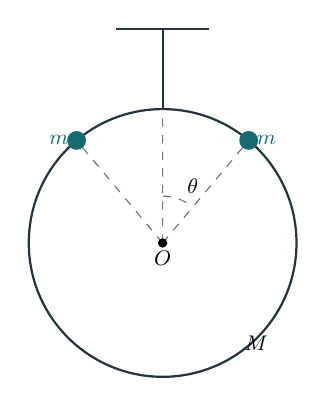
\begin{tikzpicture}[scale=.85,transform shape]

\draw[object] (0,0) circle (2);
\draw[object] (0,2)--(0,3.2);
\draw[object] (-.7,3.2)--(.7,3.2);
\fill[accent] (50:2) circle (4pt) node[right] {$m$};
\fill[accent] (130:2) circle (4pt) node[left] {$m$};
\draw[guide] (0,0)--(50:2) (0,0)--(130:2) (0,0)--(0,2);
\draw[guide] (0,.7) arc[start angle=90,end angle=50,radius=.7];
\node at (.45,.85) {$\theta$};
\fill (0,0) circle (2pt) node[below] {$O$};
\node at (1.4,-1.5) {$M$};

\end{tikzpicture}
\figcaption{图综五.3\quad 两珠穿环形成双向约束，悬绳只能提供向上拉力。}
\end{minipage}\end{center}

\Needspace{8\baselineskip}

\pdfbookmark[3]{题型定位}{q3-h0}

\subsection*{题型定位}

双向穿环约束与只受拉悬绳组成的约束转换。先用固定环能量和径向受力得到张力抛物线，确定其最低点及首次零点；再说明相切临界与穿越零轴的区别，并用首次松绳后的耦合方程证明超阈值时的向上位移。

\Needspace{8\baselineskip}

\pdfbookmark[3]{知识点}{q3-h1}

\subsection*{知识点}

\begin{itemize}
\item 穿环珠的径向力$N$可正可负，悬绳张力$T$则满足$T\ge0$。两个约束分别作用于珠与环，方向约定各自保留。
\item 固定环时小珠能量守恒给$v^2=2gR(1-x)$，径向牛顿式给$N=mg(3x-2)$；反作用的竖直投影还需乘$x$。
\item 张力配方给顶点$x=1/3$及最低值$Mg-2mg/3$。临界曲线相切，超阈值的曲线穿越零轴；时间方向对应$x$从1减小。
\item 松绳后环与珠共同运动，动能含$\dot Y\dot\theta$交叉项。首次零张力时$\ddot Y=0$，随后正的三阶时间导数给出向上位移。
\end{itemize}

\Needspace{8\baselineskip}

\pdfbookmark[3]{物理图像}{q3-h2}

\subsection*{物理图像}

\begin{itemize}
\item 图A将环对珠的径向力与珠对环的反力分开，左右珠的水平分量抵消，竖直分量相加。$N$变号时由推变拉，穿环约束继续成立。
\item 图B画固定环所需张力，穿零后的负段描绘该固定假设所需的向下作用；实际绳已松，张力取零。图C的临界曲线只在顶点触零，其余位置保持正值。
\item 图D以环中心位移$Y$和相对角$\theta$描述松绳过程，珠的惯性系竖直坐标为$Y+R\cos\theta$。这个图中两种运动共同进入速度与动能。
\end{itemize}

\Needspace{8\baselineskip}

\pdfbookmark[3]{解题入口}{q3-h3}

\subsection*{解题入口}

\begin{itemize}
\item 选$N$径向向外为正，先消去$v$，再对环写反作用。两珠对环的竖直力为$-2Nx$，与$2mg$直接替代的做法有本质区别。
\item 将$T$配方，先读出形式上的极小值，再施加绳的受拉条件。临界单独保留等号，说明固定环解仍满足全部条件。
\item 超过阈值时求两根并沿$x$减小的方向取较大根。随后写出图D的耦合坐标，比较$\dot T_{\rm fixed}$与松绳后$Y^{(3)}$的符号，完成“实际会上升”的推理。
\end{itemize}

\Needspace{8\baselineskip}

\pdfbookmark[3]{标准解法}{q3-h4}

\subsection*{标准解法}


图综五.3的两颗珠始终穿在环上，径向约束可以改变符号。两珠精确位于顶点且速度为零时，理想系统有静止平衡解；以下取微小对称扰动后开始滑动、起点趋于顶端且初始能量趋于零的极限。
\begin{center}\begin{minipage}{.98\linewidth}\centering
\begin{tikzpicture}[scale=.8,transform shape]

\draw[object] (0,0) circle (2);
\fill (1,1.732) circle (4pt) node[right] {右珠};
\draw[guide] (0,0)--(1,1.732);
\draw[force] (1,1.732)--(1.5,2.598) node[above] {$N>0$向外};
\draw[force,color=warm] (1,1.732)--(1,.45) node[right] {$mg$};
\begin{scope}[xshift=6cm]
\draw[object] (0,0) circle (1.3);
\draw[force] (0,1.3)--(0,2.7) node[above] {$T$};
\draw[force,color=warm] (0,0)--(0,-1.5) node[below] {$Mg$};
\draw[force] (.65,1.126)--(.15,.26);
\draw[force] (-.65,1.126)--(-.15,.26);
\node at (0,-2.5) {两珠反作用竖分量合为$-2Nx$};
\end{scope}

\end{tikzpicture}
\figcaption{解图综五.3A\quad 珠的径向力与环的反作用分开列式；$N<0$时环向内拉珠。}
\end{minipage}\end{center}
解图综五.3A先把环看作静止。小珠从顶端下降高度$R(1-\cos\theta)$，能量守恒给
\[
\frac12mv^2=mgR(1-\cos\theta),\qquad
v^2=2gR(1-x).
\]
规定环对珠的径向向外约束力为$N$，径向向内列牛顿方程：
\[
mg\cos\theta-N=\frac{mv^2}{R},
\qquad
\boxed{N=mg(3x-2)}.
\]
所以$x>2/3$时$N>0$，环向外推珠；$x<2/3$时$N<0$，环向内拉珠。由于珠穿在环上，$N<0$表示环向内拉珠，穿环约束仍成立。

两珠对环的水平反力相消，竖直反力之和为$-2Nx$。环仍静止时有
\[
T-Mg-2Nx=0,
\]
因而
\[
\boxed{T_{\rm fixed}(x)=Mg+2mg(3x^2-2x)
=Mg-\frac23mg+6mg\left(x-\frac13\right)^2}.
\]
由抛物线顶点，
\[
\boxed{x_{\min}=\frac13,\quad
\theta_{\min}=\arccos\frac13\simeq70.53^\circ,\quad
T_{\min}=Mg-\frac23mg}.
\]
\begin{center}\begin{minipage}{.98\linewidth}\centering
\begin{tikzpicture}[scale=.8,transform shape]

\draw[axis] (-3,0)--(3.6,0) node[right] {$x=\cos\theta$};
\draw[axis] (0,-1)--(0,6.2) node[above] {$T_{\rm fixed}/Mg$};
\draw[traj,domain=-1:1,samples=120] plot ({3*\x},{.18*(1+2*(3*\x*\x-2*\x))});
\draw[guide,color=warm,domain=-1:1,samples=120] plot ({3*\x},{.18*(1+6*(3*\x*\x-2*\x))});
\node[below] at (-3,0) {$-1$};\node[below] at (3,0) {$1$};
\node[left] at (0,.18) {$1$};
\node[text=accent] at (4.8,1.5) {$m/M=1$};
\node[text=warm] at (4.8,3) {$m/M=3$};
\node at (1.5,-1.8) {虚线负段给维持环固定所需的向下作用；松绳后$T=0$};

\end{tikzpicture}
\figcaption{解图综五.3B\quad 固定环所需张力是抛物线；曲线穿零后转入松绳运动。}
\end{minipage}\end{center}
解图综五.3B画的是“环固定”假设所需的张力。轻绳沿绳向上拉环，实际张力满足$T\ge0$；当$T_{\rm fixed}<0$时，维持环固定需要向下作用，环因而转入松绳运动。若$m/M<3/2$，整条曲线为正，绳可保持绷紧，圆环不必上升。

临界$m/M=3/2$时
\[
\boxed{T_{\rm crit}=Mg(3x-1)^2}.
\]
解图综五.3C中的抛物线在$x=1/3$处与横轴相切；$x=1$时$T=4Mg$，$x=-1$时$T=16Mg$。这个临界系统只在一个瞬间需要零张力，之后仍需要正张力，保持环静止始终满足单边约束。因此临界比是实际上升条件的下确界；在精确理想模型下，等号本身不产生有限上升。
\begin{center}\begin{minipage}{.98\linewidth}\centering
\begin{tikzpicture}[scale=.8,transform shape]

\draw[axis] (-3,0)--(3.6,0) node[right] {$x$};
\draw[axis] (0,0)--(0,5.5) node[above] {$T/Mg$};
\draw[traj,domain=-1:1,samples=160] plot ({3*\x},{.3*(3*\x-1)^2});
\draw[guide] (1,0)--(1,1.3);
\node[below] at (1,0) {$1/3$};
\node[below] at (-3,0) {$-1$};\node[below] at (3,0) {$1$};
\draw[guide] (-3,4.8)--(0,4.8) node[right] {$16$};
\draw[guide] (0,1.2)--(3,1.2);\node[left] at (0,1.2) {$4$};
\node at (4.8,3.5) {$T=Mg(3x-1)^2$};
\node at (4.8,2.3) {$m/M=3/2$};
\node at (1.5,-1.3) {临界仅瞬时触零；实际上升须$m/M>3/2$};

\end{tikzpicture}
\figcaption{解图综五.3C\quad 临界曲线与横轴相切，触零与有限上升不是同一条件。}
\end{minipage}\end{center}
实际向上离开悬挂位置要求一段运动中固定环公式需负张力，即
\[
\boxed{\frac mM>\frac32}.
\]
随着珠下滑，$x$从1减小，首次到达$T_{\rm fixed}=0$的是二次方程的较大根：
\[
3x^2-2x+\frac{M}{2m}=0,\qquad
\boxed{x_+=\frac{1+\sqrt{1-3M/(2m)}}3}.
\]
故首次松绳角为
\[
\boxed{\theta_{\rm lift}=\arccos x_+}.
\]
刚过此角时，珠对环的向上作用超过环重，绳松弛、$T=0$，圆环获得向上加速度；此后环会运动，珠的能量及约束方程都须重新写，固定环抛物线只提供首次松绳的初值，之后由珠与环的耦合运动确定。令$m/M\to(3/2)^+$，首次松绳角趋向$70.53^\circ$，这才是临界角的上升极限含义。

\textbf{首次松绳后的向上运动。} 为把负张力区与实际运动联系起来，解图综五.3D将圆环中心的竖直位移记为$Y$，向上取正。两珠相对中心的坐标分别为$(\pm R\sin\theta,R\cos\theta)$，所以惯性系中的位置是$(\pm R\sin\theta,Y+R\cos\theta)$。对两颗珠一起计算，动能和势能分别为
\[
K=\frac12(M+2m)\dot Y^2-2mR\sin\theta\,\dot Y\dot\theta
+mR^2\dot\theta^2,\qquad
V=(M+2m)gY+2mgR\cos\theta.
\]
交叉项来自珠的竖直速度$\dot Y-R\sin\theta\,\dot\theta$；它具体说明了环运动后珠速与固定环计算的区别。
\begin{center}\begin{minipage}{.98\linewidth}\centering
\begin{tikzpicture}[scale=0.72,transform shape]
\draw[object] (0,.5) circle (2);
\draw[guide] (-2.6,0)--(2.6,0);
\fill (0,.5) circle (2pt) node[below right] {$C$};
\draw[guide] (0,.5)--(0,2.5);
\foreach \x in {-1.7320508,1.7320508}{\fill[accent] (\x,1.5) circle (3pt);\draw[guide] (0,.5)--(\x,1.5);}
\draw[guide] (0,1.2) arc[start angle=90,end angle=30,radius=.7];
\node at (.65,1.3) {$\theta$};
\draw[motion] (-3.1,0)--(-3.1,.5) node[midway,left] {$Y$};
\node[align=left] at (5,.5) {两珠坐标\\$(\pm R\sin\theta,Y+R\cos\theta)$\\$\dot z=\dot Y-R\sin\theta\,\dot\theta$};
\node[below] at (0,-1.7) {松绳后以环中心平动与珠相对运动共同描述};\end{tikzpicture}
\figcaption{解图综五.3D\quad 环中心上移与珠在环上滑动共同进入惯性系速度}
\end{minipage}\end{center}
对$Y,\theta$分别写动力学关系，得到
\[
(M+2m)\ddot Y-2mR(\sin\theta\,\ddot\theta+
\cos\theta\,\dot\theta^2)=T-(M+2m)g,
\quad
R\ddot\theta=(g+\ddot Y)\sin\theta.
\]
松绳时取$T=0$，消去$\ddot\theta$得
\[
\ddot Y=-g+
\frac{2mR\cos\theta\,\dot\theta^2}{M+2m\cos^2\theta}.
\]
首次松绳恰在$x=x_+$，当时环尚未移动，$\dot Y=0$、$R\dot\theta^2=2g(1-x_+)$。代入可见$\ddot Y=0$：约束转换瞬间的加速度也连续，向上运动由随后变化的珠位置与速度产生。

令$t_*$为首次松绳时刻。在它的右侧，$\theta,\dot\theta$起初与固定环过程有相同的一阶变化，所以
\[
Y^{(3)}(t_*+)
=-\frac{\dot T_{\rm fixed}(t_*)}{M+2mx_+^2}.
\]
超阈值时$x_+>1/3$，$dT_{\rm fixed}/dx=12mg(x_+-1/3)>0$，而$\dot x=-\sin\theta\,\dot\theta<0$，故$\dot T_{\rm fixed}<0$，上式严格为正。因而短时位移为
\[
Y(t_*+\Delta t)
=-\frac{\dot T_{\rm fixed}(t_*)}{6(M+2mx_+^2)}
(\Delta t)^3+O((\Delta t)^4)>0.
\]
这给出严格质量比$m/M>3/2$下确有一段向上运动的局部证明。在等号处，两根合并且$\dot T_{\rm fixed}=0$，固定环解的张力始终非负，与悬绳的条件一致；临界点只提供向上运动的极限阈值。


\Needspace{8\baselineskip}

\pdfbookmark[3]{关键洞察}{q3-h5}

\subsection*{关键洞察}

\begin{itemize}
\item $N$的正负记录穿环的推拉，$T$的正负限制悬绳是否继续绷紧。负$N$仍是允许的真实约束力，负的固定环张力则要求转换运动状态。
\item 临界比$3/2$是能够产生有限上升的质量比集合的下确界。等号使抛物线相切，严格大于才产生负区和向上运动。
\item 首次松绳时环速、环加速度均为零，正的三阶导数使位移按短时间的三次方起始。这个连续转换与“张力刚降到零便已有有限加速度”的直觉有区别。
\end{itemize}

\Needspace{8\baselineskip}

\pdfbookmark[3]{易错点}{q3-h6}

\subsection*{易错点}

\begin{itemize}
\item 将$N=0$判为珠离开圆环，会把穿环约束改成单侧接触。只有放在外表面的球才在支持力零处脱离。
\item 漏掉反力投影中的$x$，会把张力错算成线性函数。图A的径向反力与竖直方向夹角就是$\theta$。
\item 负的$T_{\rm fixed}$属于固定环假设所需的力，实际绳张力仍为零；临界的孤立零点则与固定环静止相容。
\item 首次零点取较大根，因$x$沿运动减小。松绳之后使用$Y,\theta$的耦合关系，固定环的速度能量式只提供转换瞬间的初值。
\end{itemize}

\Needspace{8\baselineskip}

\pdfbookmark[3]{课堂讲解建议}{q3-h7}

\subsection*{课堂讲解建议}

\begin{itemize}
\item 在两张受力图上分别问哪个力允许变号，让学生说明穿环孔与轻绳各能提供什么作用。答环对珠可径向推或拉，故$N$可变号；轻绳向上拉环，故$T\ge0$。随后按反作用和投影完成环的竖直受力式。
\item 画质量比略小、等于、略大于$3/2$的三条曲线，从$x=1$向左追踪。比较全正、相切和穿越三个情形，追问临界相切时为何环可一直静止。答固定环解所需张力始终非负，只在顶点瞬时为零，整个过程仍满足悬绳受拉条件。
\item 对超阈值首次零点求环的加速度，学生会得到零。再对时间变化求导，说明为何随后仍产生向上位移，使代数阈值与实际运动联系起来。再问松绳后哪些关系需要重写，答环固定条件及据此得到的小珠速度能量式须改用$Y,\theta$的耦合关系。
\item 将穿环珠改为外表面接触球，先找$x=2/3$的脱离点，再比较张力最低点$x=1/3$，讨论模型改变后哪些后续位置仍可到达。
\end{itemize}

\Needspace{8\baselineskip}

\pdfbookmark[3]{变式训练}{q3-h8}

\subsection*{变式训练}

\begin{enumerate}
\Needspace{37\baselineskip}
\item \textbf{题设与求解。} 取$m/M=1$，求全程张力及最小值。$T/(Mg)=1+6x^2-4x=1/3+6(x-1/3)^2$，所以最低值为$Mg/3>0$，悬绳始终可保持绷紧。图V1画全区间抛物线，顶点仍位于$x=1/3$。珠在上半圆时，作用于环的竖直反力可向上或向下；是否松绳取决于其大小与环重的比较。
\begin{center}\begin{minipage}{.98\linewidth}\centering
\begin{tikzpicture}[scale=0.72,transform shape]
\draw[axis] (0,0)--(6.2,0);\draw[axis] (0,0)--(0,3.4000000000000004);
\draw[thin,color=muted] (0.0000000,0)--(0.0000000,-.07);\node[below] at (0.0000000,-.09) {$-1$};
\draw[thin,color=muted] (4.0000000,0)--(4.0000000,-.07);\node[below] at (4.0000000,-.09) {$1/3$};
\draw[thin,color=muted] (6.0000000,0)--(6.0000000,-.07);\node[below] at (6.0000000,-.09) {$1$};
\draw[thin,color=muted] (0,0.0000000)--(-.07,0.0000000);\node[left] at (-.09,0.0000000) {$0$};
\draw[thin,color=muted] (0,0.0927536)--(-.07,0.0927536);\node[left] at (-.09,0.0927536) {$1/3$};
\draw[thin,color=muted] (0,0.8347826)--(-.07,0.8347826);\node[left] at (-.09,0.8347826) {$3$};
\draw[thin,color=muted] (0,3.0608696)--(-.07,3.0608696);\node[left] at (-.09,3.0608696) {$11$};
\node[below] at (3.0,-.64) {$x=\cos\theta$};\node[above right] at (0,3.45) {$T_{\rm fixed}/(Mg)$};
\draw[traj] plot coordinates {(0.0000000,3.0608696) (0.0200000,3.0312626) (0.0400000,3.0018041) (0.0600000,2.9724939) (0.0800000,2.9433322) (0.1000000,2.9143188) (0.1200000,2.8854539) (0.1400000,2.8567374) (0.1600000,2.8281693) (0.1800000,2.7997496) (0.2000000,2.7714783) (0.2200000,2.7433554) (0.2400000,2.7153809) (0.2600000,2.6875548) (0.2800000,2.6598771) (0.3000000,2.6323478) (0.3200000,2.6049670) (0.3400000,2.5777345) (0.3600000,2.5506504) (0.3800000,2.5237148) (0.4000000,2.4969275) (0.4200000,2.4702887) (0.4400000,2.4437983) (0.4600000,2.4174562) (0.4800000,2.3912626) (0.5000000,2.3652174) (0.5200000,2.3393206) (0.5400000,2.3135722) (0.5600000,2.2879722) (0.5800000,2.2625206) (0.6000000,2.2372174) (0.6200000,2.2120626) (0.6400000,2.1870562) (0.6600000,2.1621983) (0.6800000,2.1374887) (0.7000000,2.1129275) (0.7200000,2.0885148) (0.7400000,2.0642504) (0.7600000,2.0401345) (0.7800000,2.0161670) (0.8000000,1.9923478) (0.8200000,1.9686771) (0.8400000,1.9451548) (0.8600000,1.9217809) (0.8800000,1.8985554) (0.9000000,1.8754783) (0.9200000,1.8525496) (0.9400000,1.8297693) (0.9600000,1.8071374) (0.9800000,1.7846539) (1.0000000,1.7623188) (1.0200000,1.7401322) (1.0400000,1.7180939) (1.0600000,1.6962041) (1.0800000,1.6744626) (1.1000000,1.6528696) (1.1200000,1.6314249) (1.1400000,1.6101287) (1.1600000,1.5889809) (1.1800000,1.5679814) (1.2000000,1.5471304) (1.2200000,1.5264278) (1.2400000,1.5058736) (1.2600000,1.4854678) (1.2800000,1.4652104) (1.3000000,1.4451014) (1.3200000,1.4251409) (1.3400000,1.4053287) (1.3600000,1.3856649) (1.3800000,1.3661496) (1.4000000,1.3467826) (1.4200000,1.3275641) (1.4400000,1.3084939) (1.4600000,1.2895722) (1.4800000,1.2707988) (1.5000000,1.2521739) (1.5200000,1.2336974) (1.5400000,1.2153693) (1.5600000,1.1971896) (1.5800000,1.1791583) (1.6000000,1.1612754) (1.6200000,1.1435409) (1.6400000,1.1259548) (1.6600000,1.1085171) (1.6800000,1.0912278) (1.7000000,1.0740870) (1.7200000,1.0570945) (1.7400000,1.0402504) (1.7600000,1.0235548) (1.7800000,1.0070075) (1.8000000,0.9906087) (1.8200000,0.9743583) (1.8400000,0.9582562) (1.8600000,0.9423026) (1.8800000,0.9264974) (1.9000000,0.9108406) (1.9200000,0.8953322) (1.9400000,0.8799722) (1.9600000,0.8647606) (1.9800000,0.8496974) (2.0000000,0.8347826) (2.0200000,0.8200162) (2.0400000,0.8053983) (2.0600000,0.7909287) (2.0800000,0.7766075) (2.1000000,0.7624348) (2.1200000,0.7484104) (2.1400000,0.7345345) (2.1600000,0.7208070) (2.1800000,0.7072278) (2.2000000,0.6937971) (2.2200000,0.6805148) (2.2400000,0.6673809) (2.2600000,0.6543954) (2.2800000,0.6415583) (2.3000000,0.6288696) (2.3200000,0.6163293) (2.3400000,0.6039374) (2.3600000,0.5916939) (2.3800000,0.5795988) (2.4000000,0.5676522) (2.4200000,0.5558539) (2.4400000,0.5442041) (2.4600000,0.5327026) (2.4800000,0.5213496) (2.5000000,0.5101449) (2.5200000,0.4990887) (2.5400000,0.4881809) (2.5600000,0.4774214) (2.5800000,0.4668104) (2.6000000,0.4563478) (2.6200000,0.4460336) (2.6400000,0.4358678) (2.6600000,0.4258504) (2.6800000,0.4159814) (2.7000000,0.4062609) (2.7200000,0.3966887) (2.7400000,0.3872649) (2.7600000,0.3779896) (2.7800000,0.3688626) (2.8000000,0.3598841) (2.8200000,0.3510539) (2.8400000,0.3423722) (2.8600000,0.3338388) (2.8800000,0.3254539) (2.9000000,0.3172174) (2.9200000,0.3091293) (2.9400000,0.3011896) (2.9600000,0.2933983) (2.9800000,0.2857554) (3.0000000,0.2782609) (3.0200000,0.2709148) (3.0400000,0.2637171) (3.0600000,0.2566678) (3.0800000,0.2497670) (3.1000000,0.2430145) (3.1200000,0.2364104) (3.1400000,0.2299548) (3.1600000,0.2236475) (3.1800000,0.2174887) (3.2000000,0.2114783) (3.2200000,0.2056162) (3.2400000,0.1999026) (3.2600000,0.1943374) (3.2800000,0.1889206) (3.3000000,0.1836522) (3.3200000,0.1785322) (3.3400000,0.1735606) (3.3600000,0.1687374) (3.3800000,0.1640626) (3.4000000,0.1595362) (3.4200000,0.1551583) (3.4400000,0.1509287) (3.4600000,0.1468475) (3.4800000,0.1429148) (3.5000000,0.1391304) (3.5200000,0.1354945) (3.5400000,0.1320070) (3.5600000,0.1286678) (3.5800000,0.1254771) (3.6000000,0.1224348) (3.6200000,0.1195409) (3.6400000,0.1167954) (3.6600000,0.1141983) (3.6800000,0.1117496) (3.7000000,0.1094493) (3.7200000,0.1072974) (3.7400000,0.1052939) (3.7600000,0.1034388) (3.7800000,0.1017322) (3.8000000,0.1001739) (3.8200000,0.0987641) (3.8400000,0.0975026) (3.8600000,0.0963896) (3.8800000,0.0954249) (3.9000000,0.0946087) (3.9200000,0.0939409) (3.9400000,0.0934214) (3.9600000,0.0930504) (3.9800000,0.0928278) (4.0000000,0.0927536) (4.0200000,0.0928278) (4.0400000,0.0930504) (4.0600000,0.0934214) (4.0800000,0.0939409) (4.1000000,0.0946087) (4.1200000,0.0954249) (4.1400000,0.0963896) (4.1600000,0.0975026) (4.1800000,0.0987641) (4.2000000,0.1001739) (4.2200000,0.1017322) (4.2400000,0.1034388) (4.2600000,0.1052939) (4.2800000,0.1072974) (4.3000000,0.1094493) (4.3200000,0.1117496) (4.3400000,0.1141983) (4.3600000,0.1167954) (4.3800000,0.1195409) (4.4000000,0.1224348) (4.4200000,0.1254771) (4.4400000,0.1286678) (4.4600000,0.1320070) (4.4800000,0.1354945) (4.5000000,0.1391304) (4.5200000,0.1429148) (4.5400000,0.1468475) (4.5600000,0.1509287) (4.5800000,0.1551583) (4.6000000,0.1595362) (4.6200000,0.1640626) (4.6400000,0.1687374) (4.6600000,0.1735606) (4.6800000,0.1785322) (4.7000000,0.1836522) (4.7200000,0.1889206) (4.7400000,0.1943374) (4.7600000,0.1999026) (4.7800000,0.2056162) (4.8000000,0.2114783) (4.8200000,0.2174887) (4.8400000,0.2236475) (4.8600000,0.2299548) (4.8800000,0.2364104) (4.9000000,0.2430145) (4.9200000,0.2497670) (4.9400000,0.2566678) (4.9600000,0.2637171) (4.9800000,0.2709148) (5.0000000,0.2782609) (5.0200000,0.2857554) (5.0400000,0.2933983) (5.0600000,0.3011896) (5.0800000,0.3091293) (5.1000000,0.3172174) (5.1200000,0.3254539) (5.1400000,0.3338388) (5.1600000,0.3423722) (5.1800000,0.3510539) (5.2000000,0.3598841) (5.2200000,0.3688626) (5.2400000,0.3779896) (5.2600000,0.3872649) (5.2800000,0.3966887) (5.3000000,0.4062609) (5.3200000,0.4159814) (5.3400000,0.4258504) (5.3600000,0.4358678) (5.3800000,0.4460336) (5.4000000,0.4563478) (5.4200000,0.4668104) (5.4400000,0.4774214) (5.4600000,0.4881809) (5.4800000,0.4990887) (5.5000000,0.5101449) (5.5200000,0.5213496) (5.5400000,0.5327026) (5.5600000,0.5442041) (5.5800000,0.5558539) (5.6000000,0.5676522) (5.6200000,0.5795988) (5.6400000,0.5916939) (5.6600000,0.6039374) (5.6800000,0.6163293) (5.7000000,0.6288696) (5.7200000,0.6415583) (5.7400000,0.6543954) (5.7600000,0.6673809) (5.7800000,0.6805148) (5.8000000,0.6937971) (5.8200000,0.7072278) (5.8400000,0.7208070) (5.8600000,0.7345345) (5.8800000,0.7484104) (5.9000000,0.7624348) (5.9200000,0.7766075) (5.9400000,0.7909287) (5.9600000,0.8053983) (5.9800000,0.8200162) (6.0000000,0.8347826)};
\draw[traj] (.1,-1.05)--(.7,-1.05);\node[right] at (.85,-1.05) {等珠质量比为1的固定环张力};\end{tikzpicture}
\figcaption{解图综五.3V1\quad 顶点最低值仍为正，悬绳全程保持受拉}
\end{minipage}\end{center}
\Needspace{37\baselineskip}
\item \textbf{题设与求解。} 取$m/M=3$，求首次松绳角。$T/(Mg)=1+18x^2-12x$，两根为$(1\pm1/\sqrt2)/3$。珠下滑时$x$从1减小，首先到较大根$x_+\simeq.5690$，故$\theta_{\rm lift}\simeq55.3^\circ$。图V2突出上半圆的两根区间，固定环所需负张力段使绳松弛；此后用耦合运动方程，所画负段只说明固定假设的转换。
\begin{center}\begin{minipage}{.98\linewidth}\centering
\begin{tikzpicture}[scale=0.72,transform shape]
\draw[axis] (0,0)--(6.2,0);\draw[axis] (0,0)--(0,3.4000000000000004);
\draw[thin,color=muted] (0.0000000,0)--(0.0000000,-.07);\node[below] at (0.0000000,-.09) {$0$};
\draw[thin,color=muted] (2.0000000,0)--(2.0000000,-.07);\node[below] at (2.0000000,-.09) {$1/3$};
\draw[thin,color=muted] (6.0000000,0)--(6.0000000,-.07);\node[below] at (6.0000000,-.09) {$1$};
\draw[thin,color=muted] (0,0.0372093)--(-.07,0.0372093);\node[left] at (-.09,0.0372093) {$-1$};
\draw[thin,color=muted] (0,0.4093023)--(-.07,0.4093023);\node[left] at (-.09,0.4093023) {$0$};
\draw[thin,color=muted] (0,3.0139535)--(-.07,3.0139535);\node[left] at (-.09,3.0139535) {$7$};
\node[below] at (3.0,-.64) {$x=\cos\theta$};\node[above right] at (0,3.45) {$T_{\rm fixed}/(Mg)$};
\draw[traj] plot coordinates {(0.0000000,0.7813953) (0.0200000,0.7665860) (0.0400000,0.7519256) (0.0600000,0.7374140) (0.0800000,0.7230512) (0.1000000,0.7088372) (0.1200000,0.6947721) (0.1400000,0.6808558) (0.1600000,0.6670884) (0.1800000,0.6534698) (0.2000000,0.6400000) (0.2200000,0.6266791) (0.2400000,0.6135070) (0.2600000,0.6004837) (0.2800000,0.5876093) (0.3000000,0.5748837) (0.3200000,0.5623070) (0.3400000,0.5498791) (0.3600000,0.5376000) (0.3800000,0.5254698) (0.4000000,0.5134884) (0.4200000,0.5016558) (0.4400000,0.4899721) (0.4600000,0.4784372) (0.4800000,0.4670512) (0.5000000,0.4558140) (0.5200000,0.4447256) (0.5400000,0.4337860) (0.5600000,0.4229953) (0.5800000,0.4123535) (0.6000000,0.4018605) (0.6200000,0.3915163) (0.6400000,0.3813209) (0.6600000,0.3712744) (0.6800000,0.3613767) (0.7000000,0.3516279) (0.7200000,0.3420279) (0.7400000,0.3325767) (0.7600000,0.3232744) (0.7800000,0.3141209) (0.8000000,0.3051163) (0.8200000,0.2962605) (0.8400000,0.2875535) (0.8600000,0.2789953) (0.8800000,0.2705860) (0.9000000,0.2623256) (0.9200000,0.2542140) (0.9400000,0.2462512) (0.9600000,0.2384372) (0.9800000,0.2307721) (1.0000000,0.2232558) (1.0200000,0.2158884) (1.0400000,0.2086698) (1.0600000,0.2016000) (1.0800000,0.1946791) (1.1000000,0.1879070) (1.1200000,0.1812837) (1.1400000,0.1748093) (1.1600000,0.1684837) (1.1800000,0.1623070) (1.2000000,0.1562791) (1.2200000,0.1504000) (1.2400000,0.1446698) (1.2600000,0.1390884) (1.2800000,0.1336558) (1.3000000,0.1283721) (1.3200000,0.1232372) (1.3400000,0.1182512) (1.3600000,0.1134140) (1.3800000,0.1087256) (1.4000000,0.1041860) (1.4200000,0.0997953) (1.4400000,0.0955535) (1.4600000,0.0914605) (1.4800000,0.0875163) (1.5000000,0.0837209) (1.5200000,0.0800744) (1.5400000,0.0765767) (1.5600000,0.0732279) (1.5800000,0.0700279) (1.6000000,0.0669767) (1.6200000,0.0640744) (1.6400000,0.0613209) (1.6600000,0.0587163) (1.6800000,0.0562605) (1.7000000,0.0539535) (1.7200000,0.0517953) (1.7400000,0.0497860) (1.7600000,0.0479256) (1.7800000,0.0462140) (1.8000000,0.0446512) (1.8200000,0.0432372) (1.8400000,0.0419721) (1.8600000,0.0408558) (1.8800000,0.0398884) (1.9000000,0.0390698) (1.9200000,0.0384000) (1.9400000,0.0378791) (1.9600000,0.0375070) (1.9800000,0.0372837) (2.0000000,0.0372093) (2.0200000,0.0372837) (2.0400000,0.0375070) (2.0600000,0.0378791) (2.0800000,0.0384000) (2.1000000,0.0390698) (2.1200000,0.0398884) (2.1400000,0.0408558) (2.1600000,0.0419721) (2.1800000,0.0432372) (2.2000000,0.0446512) (2.2200000,0.0462140) (2.2400000,0.0479256) (2.2600000,0.0497860) (2.2800000,0.0517953) (2.3000000,0.0539535) (2.3200000,0.0562605) (2.3400000,0.0587163) (2.3600000,0.0613209) (2.3800000,0.0640744) (2.4000000,0.0669767) (2.4200000,0.0700279) (2.4400000,0.0732279) (2.4600000,0.0765767) (2.4800000,0.0800744) (2.5000000,0.0837209) (2.5200000,0.0875163) (2.5400000,0.0914605) (2.5600000,0.0955535) (2.5800000,0.0997953) (2.6000000,0.1041860) (2.6200000,0.1087256) (2.6400000,0.1134140) (2.6600000,0.1182512) (2.6800000,0.1232372) (2.7000000,0.1283721) (2.7200000,0.1336558) (2.7400000,0.1390884) (2.7600000,0.1446698) (2.7800000,0.1504000) (2.8000000,0.1562791) (2.8200000,0.1623070) (2.8400000,0.1684837) (2.8600000,0.1748093) (2.8800000,0.1812837) (2.9000000,0.1879070) (2.9200000,0.1946791) (2.9400000,0.2016000) (2.9600000,0.2086698) (2.9800000,0.2158884) (3.0000000,0.2232558) (3.0200000,0.2307721) (3.0400000,0.2384372) (3.0600000,0.2462512) (3.0800000,0.2542140) (3.1000000,0.2623256) (3.1200000,0.2705860) (3.1400000,0.2789953) (3.1600000,0.2875535) (3.1800000,0.2962605) (3.2000000,0.3051163) (3.2200000,0.3141209) (3.2400000,0.3232744) (3.2600000,0.3325767) (3.2800000,0.3420279) (3.3000000,0.3516279) (3.3200000,0.3613767) (3.3400000,0.3712744) (3.3600000,0.3813209) (3.3800000,0.3915163) (3.4000000,0.4018605) (3.4200000,0.4123535) (3.4400000,0.4229953) (3.4600000,0.4337860) (3.4800000,0.4447256) (3.5000000,0.4558140) (3.5200000,0.4670512) (3.5400000,0.4784372) (3.5600000,0.4899721) (3.5800000,0.5016558) (3.6000000,0.5134884) (3.6200000,0.5254698) (3.6400000,0.5376000) (3.6600000,0.5498791) (3.6800000,0.5623070) (3.7000000,0.5748837) (3.7200000,0.5876093) (3.7400000,0.6004837) (3.7600000,0.6135070) (3.7800000,0.6266791) (3.8000000,0.6400000) (3.8200000,0.6534698) (3.8400000,0.6670884) (3.8600000,0.6808558) (3.8800000,0.6947721) (3.9000000,0.7088372) (3.9200000,0.7230512) (3.9400000,0.7374140) (3.9600000,0.7519256) (3.9800000,0.7665860) (4.0000000,0.7813953) (4.0200000,0.7963535) (4.0400000,0.8114605) (4.0600000,0.8267163) (4.0800000,0.8421209) (4.1000000,0.8576744) (4.1200000,0.8733767) (4.1400000,0.8892279) (4.1600000,0.9052279) (4.1800000,0.9213767) (4.2000000,0.9376744) (4.2200000,0.9541209) (4.2400000,0.9707163) (4.2600000,0.9874605) (4.2800000,1.0043535) (4.3000000,1.0213953) (4.3200000,1.0385860) (4.3400000,1.0559256) (4.3600000,1.0734140) (4.3800000,1.0910512) (4.4000000,1.1088372) (4.4200000,1.1267721) (4.4400000,1.1448558) (4.4600000,1.1630884) (4.4800000,1.1814698) (4.5000000,1.2000000) (4.5200000,1.2186791) (4.5400000,1.2375070) (4.5600000,1.2564837) (4.5800000,1.2756093) (4.6000000,1.2948837) (4.6200000,1.3143070) (4.6400000,1.3338791) (4.6600000,1.3536000) (4.6800000,1.3734698) (4.7000000,1.3934884) (4.7200000,1.4136558) (4.7400000,1.4339721) (4.7600000,1.4544372) (4.7800000,1.4750512) (4.8000000,1.4958140) (4.8200000,1.5167256) (4.8400000,1.5377860) (4.8600000,1.5589953) (4.8800000,1.5803535) (4.9000000,1.6018605) (4.9200000,1.6235163) (4.9400000,1.6453209) (4.9600000,1.6672744) (4.9800000,1.6893767) (5.0000000,1.7116279) (5.0200000,1.7340279) (5.0400000,1.7565767) (5.0600000,1.7792744) (5.0800000,1.8021209) (5.1000000,1.8251163) (5.1200000,1.8482605) (5.1400000,1.8715535) (5.1600000,1.8949953) (5.1800000,1.9185860) (5.2000000,1.9423256) (5.2200000,1.9662140) (5.2400000,1.9902512) (5.2600000,2.0144372) (5.2800000,2.0387721) (5.3000000,2.0632558) (5.3200000,2.0878884) (5.3400000,2.1126698) (5.3600000,2.1376000) (5.3800000,2.1626791) (5.4000000,2.1879070) (5.4200000,2.2132837) (5.4400000,2.2388093) (5.4600000,2.2644837) (5.4800000,2.2903070) (5.5000000,2.3162791) (5.5200000,2.3424000) (5.5400000,2.3686698) (5.5600000,2.3950884) (5.5800000,2.4216558) (5.6000000,2.4483721) (5.6200000,2.4752372) (5.6400000,2.5022512) (5.6600000,2.5294140) (5.6800000,2.5567256) (5.7000000,2.5841860) (5.7200000,2.6117953) (5.7400000,2.6395535) (5.7600000,2.6674605) (5.7800000,2.6955163) (5.8000000,2.7237209) (5.8200000,2.7520744) (5.8400000,2.7805767) (5.8600000,2.8092279) (5.8800000,2.8380279) (5.9000000,2.8669767) (5.9200000,2.8960744) (5.9400000,2.9253209) (5.9600000,2.9547163) (5.9800000,2.9842605) (6.0000000,3.0139535)};
\draw[traj] (.1,-1.05)--(.7,-1.05);\node[right] at (.85,-1.05) {质量比为3的固定假设张力};\end{tikzpicture}
\figcaption{解图综五.3V2\quad 沿$x$减小首先遇到较大零点，负段对应固定假设失效}
\end{minipage}\end{center}
\Needspace{37\baselineskip}
\item \textbf{题设与求解。} 改成两个球只接触环的外表面，求首次脱离位置。此时支持力只允许$N\ge0$，$N=mg(3x-2)$减至零时$x=2/3$、$\theta=\arccos(2/3)\simeq48.2^\circ$，随后圆周约束结束。图V3只在可接触的$2/3\le x\le1$画$N$，穿环模型张力的最低点$x=1/3$位于该段之外。在首次脱离前$x>0,N\ge0$，球对环的竖直作用向下，绳保持正张力。
\begin{center}\begin{minipage}{.98\linewidth}\centering
\begin{tikzpicture}[scale=0.72,transform shape]
\draw[axis] (0,0)--(6.2,0);\draw[axis] (0,0)--(0,3.4000000000000004);
\draw[thin,color=muted] (0.0000000,0)--(0.0000000,-.07);\node[below] at (0.0000000,-.09) {$0$};
\draw[thin,color=muted] (2.0000000,0)--(2.0000000,-.07);\node[below] at (2.0000000,-.09) {$1/3$};
\draw[thin,color=muted] (4.0000000,0)--(4.0000000,-.07);\node[below] at (4.0000000,-.09) {$2/3$};
\draw[thin,color=muted] (6.0000000,0)--(6.0000000,-.07);\node[below] at (6.0000000,-.09) {$1$};
\draw[thin,color=muted] (0,0.0000000)--(-.07,0.0000000);\node[left] at (-.09,0.0000000) {$0$};
\draw[thin,color=muted] (0,2.9090909)--(-.07,2.9090909);\node[left] at (-.09,2.9090909) {$1$};
\node[below] at (3.0,-.64) {$x=\cos\theta$};\node[above right] at (0,3.45) {$N/(mg)$};
\draw[traj] plot coordinates {(4.0000000,0.0000000) (4.0083333,0.0121212) (4.0166667,0.0242424) (4.0250000,0.0363636) (4.0333333,0.0484848) (4.0416667,0.0606061) (4.0500000,0.0727273) (4.0583333,0.0848485) (4.0666667,0.0969697) (4.0750000,0.1090909) (4.0833333,0.1212121) (4.0916667,0.1333333) (4.1000000,0.1454545) (4.1083333,0.1575758) (4.1166667,0.1696970) (4.1250000,0.1818182) (4.1333333,0.1939394) (4.1416667,0.2060606) (4.1500000,0.2181818) (4.1583333,0.2303030) (4.1666667,0.2424242) (4.1750000,0.2545455) (4.1833333,0.2666667) (4.1916667,0.2787879) (4.2000000,0.2909091) (4.2083333,0.3030303) (4.2166667,0.3151515) (4.2250000,0.3272727) (4.2333333,0.3393939) (4.2416667,0.3515152) (4.2500000,0.3636364) (4.2583333,0.3757576) (4.2666667,0.3878788) (4.2750000,0.4000000) (4.2833333,0.4121212) (4.2916667,0.4242424) (4.3000000,0.4363636) (4.3083333,0.4484848) (4.3166667,0.4606061) (4.3250000,0.4727273) (4.3333333,0.4848485) (4.3416667,0.4969697) (4.3500000,0.5090909) (4.3583333,0.5212121) (4.3666667,0.5333333) (4.3750000,0.5454545) (4.3833333,0.5575758) (4.3916667,0.5696970) (4.4000000,0.5818182) (4.4083333,0.5939394) (4.4166667,0.6060606) (4.4250000,0.6181818) (4.4333333,0.6303030) (4.4416667,0.6424242) (4.4500000,0.6545455) (4.4583333,0.6666667) (4.4666667,0.6787879) (4.4750000,0.6909091) (4.4833333,0.7030303) (4.4916667,0.7151515) (4.5000000,0.7272727) (4.5083333,0.7393939) (4.5166667,0.7515152) (4.5250000,0.7636364) (4.5333333,0.7757576) (4.5416667,0.7878788) (4.5500000,0.8000000) (4.5583333,0.8121212) (4.5666667,0.8242424) (4.5750000,0.8363636) (4.5833333,0.8484848) (4.5916667,0.8606061) (4.6000000,0.8727273) (4.6083333,0.8848485) (4.6166667,0.8969697) (4.6250000,0.9090909) (4.6333333,0.9212121) (4.6416667,0.9333333) (4.6500000,0.9454545) (4.6583333,0.9575758) (4.6666667,0.9696970) (4.6750000,0.9818182) (4.6833333,0.9939394) (4.6916667,1.0060606) (4.7000000,1.0181818) (4.7083333,1.0303030) (4.7166667,1.0424242) (4.7250000,1.0545455) (4.7333333,1.0666667) (4.7416667,1.0787879) (4.7500000,1.0909091) (4.7583333,1.1030303) (4.7666667,1.1151515) (4.7750000,1.1272727) (4.7833333,1.1393939) (4.7916667,1.1515152) (4.8000000,1.1636364) (4.8083333,1.1757576) (4.8166667,1.1878788) (4.8250000,1.2000000) (4.8333333,1.2121212) (4.8416667,1.2242424) (4.8500000,1.2363636) (4.8583333,1.2484848) (4.8666667,1.2606061) (4.8750000,1.2727273) (4.8833333,1.2848485) (4.8916667,1.2969697) (4.9000000,1.3090909) (4.9083333,1.3212121) (4.9166667,1.3333333) (4.9250000,1.3454545) (4.9333333,1.3575758) (4.9416667,1.3696970) (4.9500000,1.3818182) (4.9583333,1.3939394) (4.9666667,1.4060606) (4.9750000,1.4181818) (4.9833333,1.4303030) (4.9916667,1.4424242) (5.0000000,1.4545455) (5.0083333,1.4666667) (5.0166667,1.4787879) (5.0250000,1.4909091) (5.0333333,1.5030303) (5.0416667,1.5151515) (5.0500000,1.5272727) (5.0583333,1.5393939) (5.0666667,1.5515152) (5.0750000,1.5636364) (5.0833333,1.5757576) (5.0916667,1.5878788) (5.1000000,1.6000000) (5.1083333,1.6121212) (5.1166667,1.6242424) (5.1250000,1.6363636) (5.1333333,1.6484848) (5.1416667,1.6606061) (5.1500000,1.6727273) (5.1583333,1.6848485) (5.1666667,1.6969697) (5.1750000,1.7090909) (5.1833333,1.7212121) (5.1916667,1.7333333) (5.2000000,1.7454545) (5.2083333,1.7575758) (5.2166667,1.7696970) (5.2250000,1.7818182) (5.2333333,1.7939394) (5.2416667,1.8060606) (5.2500000,1.8181818) (5.2583333,1.8303030) (5.2666667,1.8424242) (5.2750000,1.8545455) (5.2833333,1.8666667) (5.2916667,1.8787879) (5.3000000,1.8909091) (5.3083333,1.9030303) (5.3166667,1.9151515) (5.3250000,1.9272727) (5.3333333,1.9393939) (5.3416667,1.9515152) (5.3500000,1.9636364) (5.3583333,1.9757576) (5.3666667,1.9878788) (5.3750000,2.0000000) (5.3833333,2.0121212) (5.3916667,2.0242424) (5.4000000,2.0363636) (5.4083333,2.0484848) (5.4166667,2.0606061) (5.4250000,2.0727273) (5.4333333,2.0848485) (5.4416667,2.0969697) (5.4500000,2.1090909) (5.4583333,2.1212121) (5.4666667,2.1333333) (5.4750000,2.1454545) (5.4833333,2.1575758) (5.4916667,2.1696970) (5.5000000,2.1818182) (5.5083333,2.1939394) (5.5166667,2.2060606) (5.5250000,2.2181818) (5.5333333,2.2303030) (5.5416667,2.2424242) (5.5500000,2.2545455) (5.5583333,2.2666667) (5.5666667,2.2787879) (5.5750000,2.2909091) (5.5833333,2.3030303) (5.5916667,2.3151515) (5.6000000,2.3272727) (5.6083333,2.3393939) (5.6166667,2.3515152) (5.6250000,2.3636364) (5.6333333,2.3757576) (5.6416667,2.3878788) (5.6500000,2.4000000) (5.6583333,2.4121212) (5.6666667,2.4242424) (5.6750000,2.4363636) (5.6833333,2.4484848) (5.6916667,2.4606061) (5.7000000,2.4727273) (5.7083333,2.4848485) (5.7166667,2.4969697) (5.7250000,2.5090909) (5.7333333,2.5212121) (5.7416667,2.5333333) (5.7500000,2.5454545) (5.7583333,2.5575758) (5.7666667,2.5696970) (5.7750000,2.5818182) (5.7833333,2.5939394) (5.7916667,2.6060606) (5.8000000,2.6181818) (5.8083333,2.6303030) (5.8166667,2.6424242) (5.8250000,2.6545455) (5.8333333,2.6666667) (5.8416667,2.6787879) (5.8500000,2.6909091) (5.8583333,2.7030303) (5.8666667,2.7151515) (5.8750000,2.7272727) (5.8833333,2.7393939) (5.8916667,2.7515152) (5.9000000,2.7636364) (5.9083333,2.7757576) (5.9166667,2.7878788) (5.9250000,2.8000000) (5.9333333,2.8121212) (5.9416667,2.8242424) (5.9500000,2.8363636) (5.9583333,2.8484848) (5.9666667,2.8606061) (5.9750000,2.8727273) (5.9833333,2.8848485) (5.9916667,2.8969697) (6.0000000,2.9090909)};
\draw[traj] (.1,-1.05)--(.7,-1.05);\node[right] at (.85,-1.05) {外表面接触球的可达约束力};\end{tikzpicture}
\figcaption{解图综五.3V3\quad 外表面球到$x=2/3$时脱离，后续穿环曲线不适用}
\end{minipage}\end{center}
\Needspace{37\baselineskip}
\item \textbf{题设与求解。} 令$m/M=(3/2)(1+\delta)$，求小正$\delta$时首次松绳角的展开。判别式给
\[
x_\pm=\frac{1\pm\sqrt{\delta/(1+\delta)}}3
=\frac13\pm\frac{\sqrt\delta}{3}+O(\delta^{3/2}).
\]
以$\theta_c=\arccos(1/3)$展开反余弦，得$\theta_{\rm lift}=\theta_c-\sqrt\delta/(2\sqrt2)+O(\delta)$。图V4画两根随$\delta$分裂的曲线，等号处合并为一个瞬时零点，负区宽度$2\sqrt{\delta/(1+\delta)}/3$按平方根增长。
\begin{center}\begin{minipage}{.98\linewidth}\centering
\begin{tikzpicture}[scale=0.72,transform shape]
\draw[axis] (0,0)--(6.2,0);\draw[axis] (0,0)--(0,3.4000000000000004);
\draw[thin,color=muted] (0.0000000,0)--(0.0000000,-.07);\node[below] at (0.0000000,-.09) {$0$};
\draw[thin,color=muted] (2.4000000,0)--(2.4000000,-.07);\node[below] at (2.4000000,-.09) {$.1$};
\draw[thin,color=muted] (6.0000000,0)--(6.0000000,-.07);\node[below] at (6.0000000,-.09) {$.25$};
\draw[thin,color=muted] (0,0.2909091)--(-.07,0.2909091);\node[left] at (-.09,0.2909091) {$.2$};
\draw[thin,color=muted] (0,1.5838384)--(-.07,1.5838384);\node[left] at (-.09,1.5838384) {$1/3$};
\draw[thin,color=muted] (0,3.0060606)--(-.07,3.0060606);\node[left] at (-.09,3.0060606) {$.48$};
\node[below] at (3.0,-.64) {超阈值参数$\delta$};\node[above right] at (0,3.45) {固定张力的两根};
\draw[traj] plot coordinates {(0.0000000,1.5838384) (0.0250000,1.6881069) (0.0500000,1.7312196) (0.0750000,1.7642491) (0.1000000,1.7920506) (0.1250000,1.8165061) (0.1500000,1.8385811) (0.1750000,1.8588497) (0.2000000,1.8776860) (0.2250000,1.8953499) (0.2500000,1.9120311) (0.2750000,1.9278725) (0.3000000,1.9429854) (0.3250000,1.9574583) (0.3500000,1.9713630) (0.3750000,1.9847587) (0.4000000,1.9976950) (0.4250000,2.0102136) (0.4500000,2.0223505) (0.4750000,2.0341366) (0.5000000,2.0455988) (0.5250000,2.0567608) (0.5500000,2.0676434) (0.5750000,2.0782651) (0.6000000,2.0886425) (0.6250000,2.0987903) (0.6500000,2.1087220) (0.6750000,2.1184496) (0.7000000,2.1279842) (0.7250000,2.1373358) (0.7500000,2.1465136) (0.7750000,2.1555260) (0.8000000,2.1643808) (0.8250000,2.1730850) (0.8500000,2.1816455) (0.8750000,2.1900682) (0.9000000,2.1983589) (0.9250000,2.2065229) (0.9500000,2.2145652) (0.9750000,2.2224905) (1.0000000,2.2303030) (1.0250000,2.2380070) (1.0500000,2.2456061) (1.0750000,2.2531040) (1.1000000,2.2605042) (1.1250000,2.2678099) (1.1500000,2.2750240) (1.1750000,2.2821495) (1.2000000,2.2891891) (1.2250000,2.2961454) (1.2500000,2.3030209) (1.2750000,2.3098178) (1.3000000,2.3165384) (1.3250000,2.3231848) (1.3500000,2.3297591) (1.3750000,2.3362632) (1.4000000,2.3426989) (1.4250000,2.3490679) (1.4500000,2.3553721) (1.4750000,2.3616129) (1.5000000,2.3677919) (1.5250000,2.3739107) (1.5500000,2.3799706) (1.5750000,2.3859730) (1.6000000,2.3919192) (1.6250000,2.3978105) (1.6500000,2.4036481) (1.6750000,2.4094332) (1.7000000,2.4151669) (1.7250000,2.4208503) (1.7500000,2.4264844) (1.7750000,2.4320703) (1.8000000,2.4376090) (1.8250000,2.4431013) (1.8500000,2.4485482) (1.8750000,2.4539505) (1.9000000,2.4593093) (1.9250000,2.4646251) (1.9500000,2.4698989) (1.9750000,2.4751315) (2.0000000,2.4803235) (2.0250000,2.4854758) (2.0500000,2.4905890) (2.0750000,2.4956638) (2.1000000,2.5007008) (2.1250000,2.5057008) (2.1500000,2.5106643) (2.1750000,2.5155920) (2.2000000,2.5204844) (2.2250000,2.5253421) (2.2500000,2.5301657) (2.2750000,2.5349558) (2.3000000,2.5397128) (2.3250000,2.5444373) (2.3500000,2.5491297) (2.3750000,2.5537906) (2.4000000,2.5584205) (2.4250000,2.5630198) (2.4500000,2.5675889) (2.4750000,2.5721284) (2.5000000,2.5766386) (2.5250000,2.5811199) (2.5500000,2.5855728) (2.5750000,2.5899977) (2.6000000,2.5943950) (2.6250000,2.5987650) (2.6500000,2.6031081) (2.6750000,2.6074247) (2.7000000,2.6117151) (2.7250000,2.6159797) (2.7500000,2.6202189) (2.7750000,2.6244329) (2.8000000,2.6286221) (2.8250000,2.6327868) (2.8500000,2.6369274) (2.8750000,2.6410440) (2.9000000,2.6451371) (2.9250000,2.6492069) (2.9500000,2.6532537) (2.9750000,2.6572778) (3.0000000,2.6612795) (3.0250000,2.6652589) (3.0500000,2.6692165) (3.0750000,2.6731524) (3.1000000,2.6770670) (3.1250000,2.6809604) (3.1500000,2.6848329) (3.1750000,2.6886847) (3.2000000,2.6925161) (3.2250000,2.6963273) (3.2500000,2.7001186) (3.2750000,2.7038900) (3.3000000,2.7076420) (3.3250000,2.7113747) (3.3500000,2.7150882) (3.3750000,2.7187828) (3.4000000,2.7224588) (3.4250000,2.7261162) (3.4500000,2.7297554) (3.4750000,2.7333764) (3.5000000,2.7369795) (3.5250000,2.7405649) (3.5500000,2.7441327) (3.5750000,2.7476831) (3.6000000,2.7512164) (3.6250000,2.7547326) (3.6500000,2.7582319) (3.6750000,2.7617146) (3.7000000,2.7651807) (3.7250000,2.7686305) (3.7500000,2.7720640) (3.7750000,2.7754816) (3.8000000,2.7788832) (3.8250000,2.7822691) (3.8500000,2.7856393) (3.8750000,2.7889942) (3.9000000,2.7923337) (3.9250000,2.7956581) (3.9500000,2.7989675) (3.9750000,2.8022620) (4.0000000,2.8055417) (4.0250000,2.8088069) (4.0500000,2.8120575) (4.0750000,2.8152938) (4.1000000,2.8185159) (4.1250000,2.8217239) (4.1500000,2.8249180) (4.1750000,2.8280982) (4.2000000,2.8312646) (4.2250000,2.8344175) (4.2500000,2.8375568) (4.2750000,2.8406828) (4.3000000,2.8437956) (4.3250000,2.8468952) (4.3500000,2.8499817) (4.3750000,2.8530554) (4.4000000,2.8561162) (4.4250000,2.8591643) (4.4500000,2.8621998) (4.4750000,2.8652228) (4.5000000,2.8682334) (4.5250000,2.8712317) (4.5500000,2.8742178) (4.5750000,2.8771918) (4.6000000,2.8801538) (4.6250000,2.8831039) (4.6500000,2.8860421) (4.6750000,2.8889687) (4.7000000,2.8918836) (4.7250000,2.8947870) (4.7500000,2.8976789) (4.7750000,2.9005595) (4.8000000,2.9034288) (4.8250000,2.9062869) (4.8500000,2.9091339) (4.8750000,2.9119699) (4.9000000,2.9147950) (4.9250000,2.9176092) (4.9500000,2.9204127) (4.9750000,2.9232054) (5.0000000,2.9259876) (5.0250000,2.9287592) (5.0500000,2.9315203) (5.0750000,2.9342711) (5.1000000,2.9370116) (5.1250000,2.9397418) (5.1500000,2.9424619) (5.1750000,2.9451719) (5.2000000,2.9478719) (5.2250000,2.9505619) (5.2500000,2.9532421) (5.2750000,2.9559125) (5.3000000,2.9585731) (5.3250000,2.9612241) (5.3500000,2.9638655) (5.3750000,2.9664974) (5.4000000,2.9691198) (5.4250000,2.9717328) (5.4500000,2.9743364) (5.4750000,2.9769308) (5.5000000,2.9795160) (5.5250000,2.9820921) (5.5500000,2.9846590) (5.5750000,2.9872170) (5.6000000,2.9897659) (5.6250000,2.9923060) (5.6500000,2.9948372) (5.6750000,2.9973597) (5.7000000,2.9998734) (5.7250000,3.0023784) (5.7500000,3.0048748) (5.7750000,3.0073627) (5.8000000,3.0098421) (5.8250000,3.0123130) (5.8500000,3.0147755) (5.8750000,3.0172297) (5.9000000,3.0196756) (5.9250000,3.0221132) (5.9500000,3.0245427) (5.9750000,3.0269640) (6.0000000,3.0293773)};
\draw[traj] (.1,-1.05)--(.7,-1.05);\node[right] at (.85,-1.05) {首次零点$x_+$};\draw[dashed,thick,color=warm] plot coordinates {(0.0000000,1.5838384) (0.0250000,1.4795699) (0.0500000,1.4364571) (0.0750000,1.4034277) (0.1000000,1.3756261) (0.1250000,1.3511707) (0.1500000,1.3290956) (0.1750000,1.3088271) (0.2000000,1.2899908) (0.2250000,1.2723268) (0.2500000,1.2556457) (0.2750000,1.2398043) (0.3000000,1.2246914) (0.3250000,1.2102184) (0.3500000,1.1963137) (0.3750000,1.1829180) (0.4000000,1.1699818) (0.4250000,1.1574632) (0.4500000,1.1453263) (0.4750000,1.1335402) (0.5000000,1.1220779) (0.5250000,1.1109159) (0.5500000,1.1000334) (0.5750000,1.0894117) (0.6000000,1.0790343) (0.6250000,1.0688865) (0.6500000,1.0589548) (0.6750000,1.0492271) (0.7000000,1.0396925) (0.7250000,1.0303409) (0.7500000,1.0211631) (0.7750000,1.0121507) (0.8000000,1.0032960) (0.8250000,0.9945917) (0.8500000,0.9860313) (0.8750000,0.9776086) (0.9000000,0.9693179) (0.9250000,0.9611539) (0.9500000,0.9531115) (0.9750000,0.9451863) (1.0000000,0.9373737) (1.0250000,0.9296698) (1.0500000,0.9220707) (1.0750000,0.9145727) (1.1000000,0.9071725) (1.1250000,0.8998669) (1.1500000,0.8926527) (1.1750000,0.8855272) (1.2000000,0.8784876) (1.2250000,0.8715313) (1.2500000,0.8646559) (1.2750000,0.8578590) (1.3000000,0.8511384) (1.3250000,0.8444919) (1.3500000,0.8379176) (1.3750000,0.8314136) (1.4000000,0.8249779) (1.4250000,0.8186088) (1.4500000,0.8123047) (1.4750000,0.8060639) (1.5000000,0.7998848) (1.5250000,0.7937661) (1.5500000,0.7877062) (1.5750000,0.7817038) (1.6000000,0.7757576) (1.6250000,0.7698663) (1.6500000,0.7640286) (1.6750000,0.7582436) (1.7000000,0.7525099) (1.7250000,0.7468265) (1.7500000,0.7411923) (1.7750000,0.7356064) (1.8000000,0.7300678) (1.8250000,0.7245755) (1.8500000,0.7191286) (1.8750000,0.7137262) (1.9000000,0.7083675) (1.9250000,0.7030516) (1.9500000,0.6977778) (1.9750000,0.6925453) (2.0000000,0.6873532) (2.0250000,0.6822010) (2.0500000,0.6770878) (2.0750000,0.6720130) (2.1000000,0.6669760) (2.1250000,0.6619760) (2.1500000,0.6570125) (2.1750000,0.6520848) (2.2000000,0.6471924) (2.2250000,0.6423347) (2.2500000,0.6375110) (2.2750000,0.6327210) (2.3000000,0.6279640) (2.3250000,0.6232395) (2.3500000,0.6185471) (2.3750000,0.6138861) (2.4000000,0.6092563) (2.4250000,0.6046570) (2.4500000,0.6000878) (2.4750000,0.5955484) (2.5000000,0.5910382) (2.5250000,0.5865568) (2.5500000,0.5821039) (2.5750000,0.5776790) (2.6000000,0.5732818) (2.6250000,0.5689118) (2.6500000,0.5645687) (2.6750000,0.5602521) (2.7000000,0.5559617) (2.7250000,0.5516970) (2.7500000,0.5474579) (2.7750000,0.5432439) (2.8000000,0.5390547) (2.8250000,0.5348899) (2.8500000,0.5307494) (2.8750000,0.5266327) (2.9000000,0.5225397) (2.9250000,0.5184699) (2.9500000,0.5144231) (2.9750000,0.5103990) (3.0000000,0.5063973) (3.0250000,0.5024178) (3.0500000,0.4984602) (3.0750000,0.4945243) (3.1000000,0.4906098) (3.1250000,0.4867164) (3.1500000,0.4828439) (3.1750000,0.4789921) (3.2000000,0.4751607) (3.2250000,0.4713495) (3.2500000,0.4675582) (3.2750000,0.4637867) (3.3000000,0.4600348) (3.3250000,0.4563021) (3.3500000,0.4525886) (3.3750000,0.4488939) (3.4000000,0.4452180) (3.4250000,0.4415605) (3.4500000,0.4379214) (3.4750000,0.4343004) (3.5000000,0.4306973) (3.5250000,0.4271119) (3.5500000,0.4235441) (3.5750000,0.4199936) (3.6000000,0.4164604) (3.6250000,0.4129442) (3.6500000,0.4094449) (3.6750000,0.4059622) (3.7000000,0.4024961) (3.7250000,0.3990463) (3.7500000,0.3956127) (3.7750000,0.3921952) (3.8000000,0.3887936) (3.8250000,0.3854077) (3.8500000,0.3820374) (3.8750000,0.3786826) (3.9000000,0.3753430) (3.9250000,0.3720186) (3.9500000,0.3687093) (3.9750000,0.3654148) (4.0000000,0.3621350) (4.0250000,0.3588699) (4.0500000,0.3556192) (4.0750000,0.3523829) (4.1000000,0.3491608) (4.1250000,0.3459528) (4.1500000,0.3427588) (4.1750000,0.3395786) (4.2000000,0.3364121) (4.2250000,0.3332593) (4.2500000,0.3301199) (4.2750000,0.3269939) (4.3000000,0.3238812) (4.3250000,0.3207816) (4.3500000,0.3176950) (4.3750000,0.3146214) (4.4000000,0.3115606) (4.4250000,0.3085125) (4.4500000,0.3054770) (4.4750000,0.3024540) (4.5000000,0.2994434) (4.5250000,0.2964451) (4.5500000,0.2934590) (4.5750000,0.2904850) (4.6000000,0.2875230) (4.6250000,0.2845729) (4.6500000,0.2816346) (4.6750000,0.2787081) (4.7000000,0.2757931) (4.7250000,0.2728898) (4.7500000,0.2699978) (4.7750000,0.2671173) (4.8000000,0.2642480) (4.8250000,0.2613898) (4.8500000,0.2585428) (4.8750000,0.2557068) (4.9000000,0.2528818) (4.9250000,0.2500675) (4.9500000,0.2472641) (4.9750000,0.2444714) (5.0000000,0.2416892) (5.0250000,0.2389176) (5.0500000,0.2361565) (5.0750000,0.2334057) (5.1000000,0.2306652) (5.1250000,0.2279350) (5.1500000,0.2252149) (5.1750000,0.2225049) (5.2000000,0.2198049) (5.2250000,0.2171149) (5.2500000,0.2144347) (5.2750000,0.2117643) (5.3000000,0.2091036) (5.3250000,0.2064527) (5.3500000,0.2038113) (5.3750000,0.2011794) (5.4000000,0.1985570) (5.4250000,0.1959440) (5.4500000,0.1933403) (5.4750000,0.1907459) (5.5000000,0.1881607) (5.5250000,0.1855847) (5.5500000,0.1830177) (5.5750000,0.1804598) (5.6000000,0.1779108) (5.6250000,0.1753708) (5.6500000,0.1728395) (5.6750000,0.1703171) (5.7000000,0.1678034) (5.7250000,0.1652983) (5.7500000,0.1628019) (5.7750000,0.1603141) (5.8000000,0.1578347) (5.8250000,0.1553638) (5.8500000,0.1529013) (5.8750000,0.1504471) (5.9000000,0.1480012) (5.9250000,0.1455635) (5.9500000,0.1431341) (5.9750000,0.1407127) (6.0000000,0.1382995)};
\draw[dashed,thick,color=warm] (.1,-1.48)--(.7,-1.48);\node[right] at (.85,-1.48) {另一零点$x_-$};\end{tikzpicture}
\figcaption{解图综五.3V4\quad 质量比略过临界，两根按$\delta$的平方根分裂}
\end{minipage}\end{center}
\Needspace{37\baselineskip}
\item \textbf{题设与求解。} 两珠到顶端时已有小的对称切向初速$v_0$，令$s=v_0^2/(gR)$、$0\le s\le1$，求新的阈值。固定环能量给$v^2=gR(s+2-2x)$，于是$N=mg(3x-2-s)$，
\[
T=Mg+2mg[3x^2-(2+s)x],\quad
x_{\min}=\frac{2+s}{6},\quad
T_{\min}=Mg-\frac{mg(2+s)^2}{6}.
\]
因此有限上升需$m/M>6/(2+s)^2$。初始张力$Mg+2mg(1-s)>0$，固定环阶段可成立。图V5取$m/M=1$，比较$s=0$与$s=.5$；后者阈值为$24/25$，使同样装载质量出现松绳。
\begin{center}\begin{minipage}{.98\linewidth}\centering
\begin{tikzpicture}[scale=0.72,transform shape]
\draw[axis] (0,0)--(6.2,0);\draw[axis] (0,0)--(0,3.4000000000000004);
\draw[thin,color=muted] (0.0000000,0)--(0.0000000,-.07);\node[below] at (0.0000000,-.09) {$0$};
\draw[thin,color=muted] (2.5000000,0)--(2.5000000,-.07);\node[below] at (2.5000000,-.09) {$5/12$};
\draw[thin,color=muted] (6.0000000,0)--(6.0000000,-.07);\node[below] at (6.0000000,-.09) {$1$};
\draw[thin,color=muted] (0,0.1000000)--(-.07,0.1000000);\node[left] at (-.09,0.1000000) {$0$};
\draw[thin,color=muted] (0,1.1000000)--(-.07,1.1000000);\node[left] at (-.09,1.1000000) {$1$};
\draw[thin,color=muted] (0,2.1000000)--(-.07,2.1000000);\node[left] at (-.09,2.1000000) {$2$};
\draw[thin,color=muted] (0,3.1000000)--(-.07,3.1000000);\node[left] at (-.09,3.1000000) {$3$};
\node[below] at (3.0,-.64) {$x=\cos\theta$};\node[above right] at (0,3.45) {$T_{\rm fixed}/(Mg)$};
\draw[traj] plot coordinates {(0.0000000,1.1000000) (0.0200000,1.0867333) (0.0400000,1.0736000) (0.0600000,1.0606000) (0.0800000,1.0477333) (0.1000000,1.0350000) (0.1200000,1.0224000) (0.1400000,1.0099333) (0.1600000,0.9976000) (0.1800000,0.9854000) (0.2000000,0.9733333) (0.2200000,0.9614000) (0.2400000,0.9496000) (0.2600000,0.9379333) (0.2800000,0.9264000) (0.3000000,0.9150000) (0.3200000,0.9037333) (0.3400000,0.8926000) (0.3600000,0.8816000) (0.3800000,0.8707333) (0.4000000,0.8600000) (0.4200000,0.8494000) (0.4400000,0.8389333) (0.4600000,0.8286000) (0.4800000,0.8184000) (0.5000000,0.8083333) (0.5200000,0.7984000) (0.5400000,0.7886000) (0.5600000,0.7789333) (0.5800000,0.7694000) (0.6000000,0.7600000) (0.6200000,0.7507333) (0.6400000,0.7416000) (0.6600000,0.7326000) (0.6800000,0.7237333) (0.7000000,0.7150000) (0.7200000,0.7064000) (0.7400000,0.6979333) (0.7600000,0.6896000) (0.7800000,0.6814000) (0.8000000,0.6733333) (0.8200000,0.6654000) (0.8400000,0.6576000) (0.8600000,0.6499333) (0.8800000,0.6424000) (0.9000000,0.6350000) (0.9200000,0.6277333) (0.9400000,0.6206000) (0.9600000,0.6136000) (0.9800000,0.6067333) (1.0000000,0.6000000) (1.0200000,0.5934000) (1.0400000,0.5869333) (1.0600000,0.5806000) (1.0800000,0.5744000) (1.1000000,0.5683333) (1.1200000,0.5624000) (1.1400000,0.5566000) (1.1600000,0.5509333) (1.1800000,0.5454000) (1.2000000,0.5400000) (1.2200000,0.5347333) (1.2400000,0.5296000) (1.2600000,0.5246000) (1.2800000,0.5197333) (1.3000000,0.5150000) (1.3200000,0.5104000) (1.3400000,0.5059333) (1.3600000,0.5016000) (1.3800000,0.4974000) (1.4000000,0.4933333) (1.4200000,0.4894000) (1.4400000,0.4856000) (1.4600000,0.4819333) (1.4800000,0.4784000) (1.5000000,0.4750000) (1.5200000,0.4717333) (1.5400000,0.4686000) (1.5600000,0.4656000) (1.5800000,0.4627333) (1.6000000,0.4600000) (1.6200000,0.4574000) (1.6400000,0.4549333) (1.6600000,0.4526000) (1.6800000,0.4504000) (1.7000000,0.4483333) (1.7200000,0.4464000) (1.7400000,0.4446000) (1.7600000,0.4429333) (1.7800000,0.4414000) (1.8000000,0.4400000) (1.8200000,0.4387333) (1.8400000,0.4376000) (1.8600000,0.4366000) (1.8800000,0.4357333) (1.9000000,0.4350000) (1.9200000,0.4344000) (1.9400000,0.4339333) (1.9600000,0.4336000) (1.9800000,0.4334000) (2.0000000,0.4333333) (2.0200000,0.4334000) (2.0400000,0.4336000) (2.0600000,0.4339333) (2.0800000,0.4344000) (2.1000000,0.4350000) (2.1200000,0.4357333) (2.1400000,0.4366000) (2.1600000,0.4376000) (2.1800000,0.4387333) (2.2000000,0.4400000) (2.2200000,0.4414000) (2.2400000,0.4429333) (2.2600000,0.4446000) (2.2800000,0.4464000) (2.3000000,0.4483333) (2.3200000,0.4504000) (2.3400000,0.4526000) (2.3600000,0.4549333) (2.3800000,0.4574000) (2.4000000,0.4600000) (2.4200000,0.4627333) (2.4400000,0.4656000) (2.4600000,0.4686000) (2.4800000,0.4717333) (2.5000000,0.4750000) (2.5200000,0.4784000) (2.5400000,0.4819333) (2.5600000,0.4856000) (2.5800000,0.4894000) (2.6000000,0.4933333) (2.6200000,0.4974000) (2.6400000,0.5016000) (2.6600000,0.5059333) (2.6800000,0.5104000) (2.7000000,0.5150000) (2.7200000,0.5197333) (2.7400000,0.5246000) (2.7600000,0.5296000) (2.7800000,0.5347333) (2.8000000,0.5400000) (2.8200000,0.5454000) (2.8400000,0.5509333) (2.8600000,0.5566000) (2.8800000,0.5624000) (2.9000000,0.5683333) (2.9200000,0.5744000) (2.9400000,0.5806000) (2.9600000,0.5869333) (2.9800000,0.5934000) (3.0000000,0.6000000) (3.0200000,0.6067333) (3.0400000,0.6136000) (3.0600000,0.6206000) (3.0800000,0.6277333) (3.1000000,0.6350000) (3.1200000,0.6424000) (3.1400000,0.6499333) (3.1600000,0.6576000) (3.1800000,0.6654000) (3.2000000,0.6733333) (3.2200000,0.6814000) (3.2400000,0.6896000) (3.2600000,0.6979333) (3.2800000,0.7064000) (3.3000000,0.7150000) (3.3200000,0.7237333) (3.3400000,0.7326000) (3.3600000,0.7416000) (3.3800000,0.7507333) (3.4000000,0.7600000) (3.4200000,0.7694000) (3.4400000,0.7789333) (3.4600000,0.7886000) (3.4800000,0.7984000) (3.5000000,0.8083333) (3.5200000,0.8184000) (3.5400000,0.8286000) (3.5600000,0.8389333) (3.5800000,0.8494000) (3.6000000,0.8600000) (3.6200000,0.8707333) (3.6400000,0.8816000) (3.6600000,0.8926000) (3.6800000,0.9037333) (3.7000000,0.9150000) (3.7200000,0.9264000) (3.7400000,0.9379333) (3.7600000,0.9496000) (3.7800000,0.9614000) (3.8000000,0.9733333) (3.8200000,0.9854000) (3.8400000,0.9976000) (3.8600000,1.0099333) (3.8800000,1.0224000) (3.9000000,1.0350000) (3.9200000,1.0477333) (3.9400000,1.0606000) (3.9600000,1.0736000) (3.9800000,1.0867333) (4.0000000,1.1000000) (4.0200000,1.1134000) (4.0400000,1.1269333) (4.0600000,1.1406000) (4.0800000,1.1544000) (4.1000000,1.1683333) (4.1200000,1.1824000) (4.1400000,1.1966000) (4.1600000,1.2109333) (4.1800000,1.2254000) (4.2000000,1.2400000) (4.2200000,1.2547333) (4.2400000,1.2696000) (4.2600000,1.2846000) (4.2800000,1.2997333) (4.3000000,1.3150000) (4.3200000,1.3304000) (4.3400000,1.3459333) (4.3600000,1.3616000) (4.3800000,1.3774000) (4.4000000,1.3933333) (4.4200000,1.4094000) (4.4400000,1.4256000) (4.4600000,1.4419333) (4.4800000,1.4584000) (4.5000000,1.4750000) (4.5200000,1.4917333) (4.5400000,1.5086000) (4.5600000,1.5256000) (4.5800000,1.5427333) (4.6000000,1.5600000) (4.6200000,1.5774000) (4.6400000,1.5949333) (4.6600000,1.6126000) (4.6800000,1.6304000) (4.7000000,1.6483333) (4.7200000,1.6664000) (4.7400000,1.6846000) (4.7600000,1.7029333) (4.7800000,1.7214000) (4.8000000,1.7400000) (4.8200000,1.7587333) (4.8400000,1.7776000) (4.8600000,1.7966000) (4.8800000,1.8157333) (4.9000000,1.8350000) (4.9200000,1.8544000) (4.9400000,1.8739333) (4.9600000,1.8936000) (4.9800000,1.9134000) (5.0000000,1.9333333) (5.0200000,1.9534000) (5.0400000,1.9736000) (5.0600000,1.9939333) (5.0800000,2.0144000) (5.1000000,2.0350000) (5.1200000,2.0557333) (5.1400000,2.0766000) (5.1600000,2.0976000) (5.1800000,2.1187333) (5.2000000,2.1400000) (5.2200000,2.1614000) (5.2400000,2.1829333) (5.2600000,2.2046000) (5.2800000,2.2264000) (5.3000000,2.2483333) (5.3200000,2.2704000) (5.3400000,2.2926000) (5.3600000,2.3149333) (5.3800000,2.3374000) (5.4000000,2.3600000) (5.4200000,2.3827333) (5.4400000,2.4056000) (5.4600000,2.4286000) (5.4800000,2.4517333) (5.5000000,2.4750000) (5.5200000,2.4984000) (5.5400000,2.5219333) (5.5600000,2.5456000) (5.5800000,2.5694000) (5.6000000,2.5933333) (5.6200000,2.6174000) (5.6400000,2.6416000) (5.6600000,2.6659333) (5.6800000,2.6904000) (5.7000000,2.7150000) (5.7200000,2.7397333) (5.7400000,2.7646000) (5.7600000,2.7896000) (5.7800000,2.8147333) (5.8000000,2.8400000) (5.8200000,2.8654000) (5.8400000,2.8909333) (5.8600000,2.9166000) (5.8800000,2.9424000) (5.9000000,2.9683333) (5.9200000,2.9944000) (5.9400000,3.0206000) (5.9600000,3.0469333) (5.9800000,3.0734000) (6.0000000,3.1000000)};
\draw[traj] (.1,-1.05)--(.7,-1.05);\node[right] at (.85,-1.05) {顶端初速零};\draw[dashed,thick,color=warm] plot coordinates {(0.0000000,1.1000000) (0.0200000,1.0834000) (0.0400000,1.0669333) (0.0600000,1.0506000) (0.0800000,1.0344000) (0.1000000,1.0183333) (0.1200000,1.0024000) (0.1400000,0.9866000) (0.1600000,0.9709333) (0.1800000,0.9554000) (0.2000000,0.9400000) (0.2200000,0.9247333) (0.2400000,0.9096000) (0.2600000,0.8946000) (0.2800000,0.8797333) (0.3000000,0.8650000) (0.3200000,0.8504000) (0.3400000,0.8359333) (0.3600000,0.8216000) (0.3800000,0.8074000) (0.4000000,0.7933333) (0.4200000,0.7794000) (0.4400000,0.7656000) (0.4600000,0.7519333) (0.4800000,0.7384000) (0.5000000,0.7250000) (0.5200000,0.7117333) (0.5400000,0.6986000) (0.5600000,0.6856000) (0.5800000,0.6727333) (0.6000000,0.6600000) (0.6200000,0.6474000) (0.6400000,0.6349333) (0.6600000,0.6226000) (0.6800000,0.6104000) (0.7000000,0.5983333) (0.7200000,0.5864000) (0.7400000,0.5746000) (0.7600000,0.5629333) (0.7800000,0.5514000) (0.8000000,0.5400000) (0.8200000,0.5287333) (0.8400000,0.5176000) (0.8600000,0.5066000) (0.8800000,0.4957333) (0.9000000,0.4850000) (0.9200000,0.4744000) (0.9400000,0.4639333) (0.9600000,0.4536000) (0.9800000,0.4434000) (1.0000000,0.4333333) (1.0200000,0.4234000) (1.0400000,0.4136000) (1.0600000,0.4039333) (1.0800000,0.3944000) (1.1000000,0.3850000) (1.1200000,0.3757333) (1.1400000,0.3666000) (1.1600000,0.3576000) (1.1800000,0.3487333) (1.2000000,0.3400000) (1.2200000,0.3314000) (1.2400000,0.3229333) (1.2600000,0.3146000) (1.2800000,0.3064000) (1.3000000,0.2983333) (1.3200000,0.2904000) (1.3400000,0.2826000) (1.3600000,0.2749333) (1.3800000,0.2674000) (1.4000000,0.2600000) (1.4200000,0.2527333) (1.4400000,0.2456000) (1.4600000,0.2386000) (1.4800000,0.2317333) (1.5000000,0.2250000) (1.5200000,0.2184000) (1.5400000,0.2119333) (1.5600000,0.2056000) (1.5800000,0.1994000) (1.6000000,0.1933333) (1.6200000,0.1874000) (1.6400000,0.1816000) (1.6600000,0.1759333) (1.6800000,0.1704000) (1.7000000,0.1650000) (1.7200000,0.1597333) (1.7400000,0.1546000) (1.7600000,0.1496000) (1.7800000,0.1447333) (1.8000000,0.1400000) (1.8200000,0.1354000) (1.8400000,0.1309333) (1.8600000,0.1266000) (1.8800000,0.1224000) (1.9000000,0.1183333) (1.9200000,0.1144000) (1.9400000,0.1106000) (1.9600000,0.1069333) (1.9800000,0.1034000) (2.0000000,0.1000000) (2.0200000,0.0967333) (2.0400000,0.0936000) (2.0600000,0.0906000) (2.0800000,0.0877333) (2.1000000,0.0850000) (2.1200000,0.0824000) (2.1400000,0.0799333) (2.1600000,0.0776000) (2.1800000,0.0754000) (2.2000000,0.0733333) (2.2200000,0.0714000) (2.2400000,0.0696000) (2.2600000,0.0679333) (2.2800000,0.0664000) (2.3000000,0.0650000) (2.3200000,0.0637333) (2.3400000,0.0626000) (2.3600000,0.0616000) (2.3800000,0.0607333) (2.4000000,0.0600000) (2.4200000,0.0594000) (2.4400000,0.0589333) (2.4600000,0.0586000) (2.4800000,0.0584000) (2.5000000,0.0583333) (2.5200000,0.0584000) (2.5400000,0.0586000) (2.5600000,0.0589333) (2.5800000,0.0594000) (2.6000000,0.0600000) (2.6200000,0.0607333) (2.6400000,0.0616000) (2.6600000,0.0626000) (2.6800000,0.0637333) (2.7000000,0.0650000) (2.7200000,0.0664000) (2.7400000,0.0679333) (2.7600000,0.0696000) (2.7800000,0.0714000) (2.8000000,0.0733333) (2.8200000,0.0754000) (2.8400000,0.0776000) (2.8600000,0.0799333) (2.8800000,0.0824000) (2.9000000,0.0850000) (2.9200000,0.0877333) (2.9400000,0.0906000) (2.9600000,0.0936000) (2.9800000,0.0967333) (3.0000000,0.1000000) (3.0200000,0.1034000) (3.0400000,0.1069333) (3.0600000,0.1106000) (3.0800000,0.1144000) (3.1000000,0.1183333) (3.1200000,0.1224000) (3.1400000,0.1266000) (3.1600000,0.1309333) (3.1800000,0.1354000) (3.2000000,0.1400000) (3.2200000,0.1447333) (3.2400000,0.1496000) (3.2600000,0.1546000) (3.2800000,0.1597333) (3.3000000,0.1650000) (3.3200000,0.1704000) (3.3400000,0.1759333) (3.3600000,0.1816000) (3.3800000,0.1874000) (3.4000000,0.1933333) (3.4200000,0.1994000) (3.4400000,0.2056000) (3.4600000,0.2119333) (3.4800000,0.2184000) (3.5000000,0.2250000) (3.5200000,0.2317333) (3.5400000,0.2386000) (3.5600000,0.2456000) (3.5800000,0.2527333) (3.6000000,0.2600000) (3.6200000,0.2674000) (3.6400000,0.2749333) (3.6600000,0.2826000) (3.6800000,0.2904000) (3.7000000,0.2983333) (3.7200000,0.3064000) (3.7400000,0.3146000) (3.7600000,0.3229333) (3.7800000,0.3314000) (3.8000000,0.3400000) (3.8200000,0.3487333) (3.8400000,0.3576000) (3.8600000,0.3666000) (3.8800000,0.3757333) (3.9000000,0.3850000) (3.9200000,0.3944000) (3.9400000,0.4039333) (3.9600000,0.4136000) (3.9800000,0.4234000) (4.0000000,0.4333333) (4.0200000,0.4434000) (4.0400000,0.4536000) (4.0600000,0.4639333) (4.0800000,0.4744000) (4.1000000,0.4850000) (4.1200000,0.4957333) (4.1400000,0.5066000) (4.1600000,0.5176000) (4.1800000,0.5287333) (4.2000000,0.5400000) (4.2200000,0.5514000) (4.2400000,0.5629333) (4.2600000,0.5746000) (4.2800000,0.5864000) (4.3000000,0.5983333) (4.3200000,0.6104000) (4.3400000,0.6226000) (4.3600000,0.6349333) (4.3800000,0.6474000) (4.4000000,0.6600000) (4.4200000,0.6727333) (4.4400000,0.6856000) (4.4600000,0.6986000) (4.4800000,0.7117333) (4.5000000,0.7250000) (4.5200000,0.7384000) (4.5400000,0.7519333) (4.5600000,0.7656000) (4.5800000,0.7794000) (4.6000000,0.7933333) (4.6200000,0.8074000) (4.6400000,0.8216000) (4.6600000,0.8359333) (4.6800000,0.8504000) (4.7000000,0.8650000) (4.7200000,0.8797333) (4.7400000,0.8946000) (4.7600000,0.9096000) (4.7800000,0.9247333) (4.8000000,0.9400000) (4.8200000,0.9554000) (4.8400000,0.9709333) (4.8600000,0.9866000) (4.8800000,1.0024000) (4.9000000,1.0183333) (4.9200000,1.0344000) (4.9400000,1.0506000) (4.9600000,1.0669333) (4.9800000,1.0834000) (5.0000000,1.1000000) (5.0200000,1.1167333) (5.0400000,1.1336000) (5.0600000,1.1506000) (5.0800000,1.1677333) (5.1000000,1.1850000) (5.1200000,1.2024000) (5.1400000,1.2199333) (5.1600000,1.2376000) (5.1800000,1.2554000) (5.2000000,1.2733333) (5.2200000,1.2914000) (5.2400000,1.3096000) (5.2600000,1.3279333) (5.2800000,1.3464000) (5.3000000,1.3650000) (5.3200000,1.3837333) (5.3400000,1.4026000) (5.3600000,1.4216000) (5.3800000,1.4407333) (5.4000000,1.4600000) (5.4200000,1.4794000) (5.4400000,1.4989333) (5.4600000,1.5186000) (5.4800000,1.5384000) (5.5000000,1.5583333) (5.5200000,1.5784000) (5.5400000,1.5986000) (5.5600000,1.6189333) (5.5800000,1.6394000) (5.6000000,1.6600000) (5.6200000,1.6807333) (5.6400000,1.7016000) (5.6600000,1.7226000) (5.6800000,1.7437333) (5.7000000,1.7650000) (5.7200000,1.7864000) (5.7400000,1.8079333) (5.7600000,1.8296000) (5.7800000,1.8514000) (5.8000000,1.8733333) (5.8200000,1.8954000) (5.8400000,1.9176000) (5.8600000,1.9399333) (5.8800000,1.9624000) (5.9000000,1.9850000) (5.9200000,2.0077333) (5.9400000,2.0306000) (5.9600000,2.0536000) (5.9800000,2.0767333) (6.0000000,2.1000000)};
\draw[dashed,thick,color=warm] (.1,-1.48)--(.7,-1.48);\node[right] at (.85,-1.48) {顶端无量纲初速平方为0.5};\end{tikzpicture}
\figcaption{解图综五.3V5\quad 同样装载质量下初始动能增加，可使固定张力进入负区}
\end{minipage}\end{center}
\Needspace{37\baselineskip}
\item \textbf{题设与求解。} 求两珠对环的竖直向上合力在哪一段为正，以及它的最大值。$F_\uparrow=-2Nx=2mg(2x-3x^2)$，故仅在$0<x<2/3$时向上，其最大值位于$x=1/3$，为$2mg/3$。图V6将径向力$N/(mg)=3x-2$与$F_\uparrow/(mg)$并列，珠对环产生拉力的范围是$x<2/3$，但进入下半圆后其竖直分量转向下方。最大向上合力超过$Mg$正好给出严格阈值$m/M>3/2$。
\begin{center}\begin{minipage}{.98\linewidth}\centering
\begin{tikzpicture}[scale=0.72,transform shape]
\draw[axis] (0,0)--(6.2,0);\draw[axis] (0,0)--(0,3.4000000000000004);
\draw[thin,color=muted] (0.0000000,0)--(0.0000000,-.07);\node[below] at (0.0000000,-.09) {$-1$};
\draw[thin,color=muted] (3.0000000,0)--(3.0000000,-.07);\node[below] at (3.0000000,-.09) {$0$};
\draw[thin,color=muted] (4.0000000,0)--(4.0000000,-.07);\node[below] at (4.0000000,-.09) {$1/3$};
\draw[thin,color=muted] (5.0000000,0)--(5.0000000,-.07);\node[below] at (5.0000000,-.09) {$2/3$};
\draw[thin,color=muted] (6.0000000,0)--(6.0000000,-.07);\node[below] at (6.0000000,-.09) {$1$};
\draw[thin,color=muted] (0,0.1355932)--(-.07,0.1355932);\node[left] at (-.09,0.1355932) {$-10$};
\draw[thin,color=muted] (0,2.8474576)--(-.07,2.8474576);\node[left] at (-.09,2.8474576) {$0$};
\draw[thin,color=muted] (0,3.0282486)--(-.07,3.0282486);\node[left] at (-.09,3.0282486) {$2/3$};
\node[below] at (3.0,-.64) {$x=\cos\theta$};\node[above right] at (0,3.45) {相应力除以$mg$};
\draw[traj] plot coordinates {(0.0000000,1.4915254) (0.0200000,1.4969492) (0.0400000,1.5023729) (0.0600000,1.5077966) (0.0800000,1.5132203) (0.1000000,1.5186441) (0.1200000,1.5240678) (0.1400000,1.5294915) (0.1600000,1.5349153) (0.1800000,1.5403390) (0.2000000,1.5457627) (0.2200000,1.5511864) (0.2400000,1.5566102) (0.2600000,1.5620339) (0.2800000,1.5674576) (0.3000000,1.5728814) (0.3200000,1.5783051) (0.3400000,1.5837288) (0.3600000,1.5891525) (0.3800000,1.5945763) (0.4000000,1.6000000) (0.4200000,1.6054237) (0.4400000,1.6108475) (0.4600000,1.6162712) (0.4800000,1.6216949) (0.5000000,1.6271186) (0.5200000,1.6325424) (0.5400000,1.6379661) (0.5600000,1.6433898) (0.5800000,1.6488136) (0.6000000,1.6542373) (0.6200000,1.6596610) (0.6400000,1.6650847) (0.6600000,1.6705085) (0.6800000,1.6759322) (0.7000000,1.6813559) (0.7200000,1.6867797) (0.7400000,1.6922034) (0.7600000,1.6976271) (0.7800000,1.7030508) (0.8000000,1.7084746) (0.8200000,1.7138983) (0.8400000,1.7193220) (0.8600000,1.7247458) (0.8800000,1.7301695) (0.9000000,1.7355932) (0.9200000,1.7410169) (0.9400000,1.7464407) (0.9600000,1.7518644) (0.9800000,1.7572881) (1.0000000,1.7627119) (1.0200000,1.7681356) (1.0400000,1.7735593) (1.0600000,1.7789831) (1.0800000,1.7844068) (1.1000000,1.7898305) (1.1200000,1.7952542) (1.1400000,1.8006780) (1.1600000,1.8061017) (1.1800000,1.8115254) (1.2000000,1.8169492) (1.2200000,1.8223729) (1.2400000,1.8277966) (1.2600000,1.8332203) (1.2800000,1.8386441) (1.3000000,1.8440678) (1.3200000,1.8494915) (1.3400000,1.8549153) (1.3600000,1.8603390) (1.3800000,1.8657627) (1.4000000,1.8711864) (1.4200000,1.8766102) (1.4400000,1.8820339) (1.4600000,1.8874576) (1.4800000,1.8928814) (1.5000000,1.8983051) (1.5200000,1.9037288) (1.5400000,1.9091525) (1.5600000,1.9145763) (1.5800000,1.9200000) (1.6000000,1.9254237) (1.6200000,1.9308475) (1.6400000,1.9362712) (1.6600000,1.9416949) (1.6800000,1.9471186) (1.7000000,1.9525424) (1.7200000,1.9579661) (1.7400000,1.9633898) (1.7600000,1.9688136) (1.7800000,1.9742373) (1.8000000,1.9796610) (1.8200000,1.9850847) (1.8400000,1.9905085) (1.8600000,1.9959322) (1.8800000,2.0013559) (1.9000000,2.0067797) (1.9200000,2.0122034) (1.9400000,2.0176271) (1.9600000,2.0230508) (1.9800000,2.0284746) (2.0000000,2.0338983) (2.0200000,2.0393220) (2.0400000,2.0447458) (2.0600000,2.0501695) (2.0800000,2.0555932) (2.1000000,2.0610169) (2.1200000,2.0664407) (2.1400000,2.0718644) (2.1600000,2.0772881) (2.1800000,2.0827119) (2.2000000,2.0881356) (2.2200000,2.0935593) (2.2400000,2.0989831) (2.2600000,2.1044068) (2.2800000,2.1098305) (2.3000000,2.1152542) (2.3200000,2.1206780) (2.3400000,2.1261017) (2.3600000,2.1315254) (2.3800000,2.1369492) (2.4000000,2.1423729) (2.4200000,2.1477966) (2.4400000,2.1532203) (2.4600000,2.1586441) (2.4800000,2.1640678) (2.5000000,2.1694915) (2.5200000,2.1749153) (2.5400000,2.1803390) (2.5600000,2.1857627) (2.5800000,2.1911864) (2.6000000,2.1966102) (2.6200000,2.2020339) (2.6400000,2.2074576) (2.6600000,2.2128814) (2.6800000,2.2183051) (2.7000000,2.2237288) (2.7200000,2.2291525) (2.7400000,2.2345763) (2.7600000,2.2400000) (2.7800000,2.2454237) (2.8000000,2.2508475) (2.8200000,2.2562712) (2.8400000,2.2616949) (2.8600000,2.2671186) (2.8800000,2.2725424) (2.9000000,2.2779661) (2.9200000,2.2833898) (2.9400000,2.2888136) (2.9600000,2.2942373) (2.9800000,2.2996610) (3.0000000,2.3050847) (3.0200000,2.3105085) (3.0400000,2.3159322) (3.0600000,2.3213559) (3.0800000,2.3267797) (3.1000000,2.3322034) (3.1200000,2.3376271) (3.1400000,2.3430508) (3.1600000,2.3484746) (3.1800000,2.3538983) (3.2000000,2.3593220) (3.2200000,2.3647458) (3.2400000,2.3701695) (3.2600000,2.3755932) (3.2800000,2.3810169) (3.3000000,2.3864407) (3.3200000,2.3918644) (3.3400000,2.3972881) (3.3600000,2.4027119) (3.3800000,2.4081356) (3.4000000,2.4135593) (3.4200000,2.4189831) (3.4400000,2.4244068) (3.4600000,2.4298305) (3.4800000,2.4352542) (3.5000000,2.4406780) (3.5200000,2.4461017) (3.5400000,2.4515254) (3.5600000,2.4569492) (3.5800000,2.4623729) (3.6000000,2.4677966) (3.6200000,2.4732203) (3.6400000,2.4786441) (3.6600000,2.4840678) (3.6800000,2.4894915) (3.7000000,2.4949153) (3.7200000,2.5003390) (3.7400000,2.5057627) (3.7600000,2.5111864) (3.7800000,2.5166102) (3.8000000,2.5220339) (3.8200000,2.5274576) (3.8400000,2.5328814) (3.8600000,2.5383051) (3.8800000,2.5437288) (3.9000000,2.5491525) (3.9200000,2.5545763) (3.9400000,2.5600000) (3.9600000,2.5654237) (3.9800000,2.5708475) (4.0000000,2.5762712) (4.0200000,2.5816949) (4.0400000,2.5871186) (4.0600000,2.5925424) (4.0800000,2.5979661) (4.1000000,2.6033898) (4.1200000,2.6088136) (4.1400000,2.6142373) (4.1600000,2.6196610) (4.1800000,2.6250847) (4.2000000,2.6305085) (4.2200000,2.6359322) (4.2400000,2.6413559) (4.2600000,2.6467797) (4.2800000,2.6522034) (4.3000000,2.6576271) (4.3200000,2.6630508) (4.3400000,2.6684746) (4.3600000,2.6738983) (4.3800000,2.6793220) (4.4000000,2.6847458) (4.4200000,2.6901695) (4.4400000,2.6955932) (4.4600000,2.7010169) (4.4800000,2.7064407) (4.5000000,2.7118644) (4.5200000,2.7172881) (4.5400000,2.7227119) (4.5600000,2.7281356) (4.5800000,2.7335593) (4.6000000,2.7389831) (4.6200000,2.7444068) (4.6400000,2.7498305) (4.6600000,2.7552542) (4.6800000,2.7606780) (4.7000000,2.7661017) (4.7200000,2.7715254) (4.7400000,2.7769492) (4.7600000,2.7823729) (4.7800000,2.7877966) (4.8000000,2.7932203) (4.8200000,2.7986441) (4.8400000,2.8040678) (4.8600000,2.8094915) (4.8800000,2.8149153) (4.9000000,2.8203390) (4.9200000,2.8257627) (4.9400000,2.8311864) (4.9600000,2.8366102) (4.9800000,2.8420339) (5.0000000,2.8474576) (5.0200000,2.8528814) (5.0400000,2.8583051) (5.0600000,2.8637288) (5.0800000,2.8691525) (5.1000000,2.8745763) (5.1200000,2.8800000) (5.1400000,2.8854237) (5.1600000,2.8908475) (5.1800000,2.8962712) (5.2000000,2.9016949) (5.2200000,2.9071186) (5.2400000,2.9125424) (5.2600000,2.9179661) (5.2800000,2.9233898) (5.3000000,2.9288136) (5.3200000,2.9342373) (5.3400000,2.9396610) (5.3600000,2.9450847) (5.3800000,2.9505085) (5.4000000,2.9559322) (5.4200000,2.9613559) (5.4400000,2.9667797) (5.4600000,2.9722034) (5.4800000,2.9776271) (5.5000000,2.9830508) (5.5200000,2.9884746) (5.5400000,2.9938983) (5.5600000,2.9993220) (5.5800000,3.0047458) (5.6000000,3.0101695) (5.6200000,3.0155932) (5.6400000,3.0210169) (5.6600000,3.0264407) (5.6800000,3.0318644) (5.7000000,3.0372881) (5.7200000,3.0427119) (5.7400000,3.0481356) (5.7600000,3.0535593) (5.7800000,3.0589831) (5.8000000,3.0644068) (5.8200000,3.0698305) (5.8400000,3.0752542) (5.8600000,3.0806780) (5.8800000,3.0861017) (5.9000000,3.0915254) (5.9200000,3.0969492) (5.9400000,3.1023729) (5.9600000,3.1077966) (5.9800000,3.1132203) (6.0000000,3.1186441)};
\draw[traj] (.1,-1.05)--(.7,-1.05);\node[right] at (.85,-1.05) {环对一珠的径向力};\draw[dashed,thick,color=warm] plot coordinates {(0.0000000,0.1355932) (0.0200000,0.1644475) (0.0400000,0.1931571) (0.0600000,0.2217220) (0.0800000,0.2501424) (0.1000000,0.2784181) (0.1200000,0.3065492) (0.1400000,0.3345356) (0.1600000,0.3623774) (0.1800000,0.3900746) (0.2000000,0.4176271) (0.2200000,0.4450350) (0.2400000,0.4722983) (0.2600000,0.4994169) (0.2800000,0.5263910) (0.3000000,0.5532203) (0.3200000,0.5799051) (0.3400000,0.6064452) (0.3600000,0.6328407) (0.3800000,0.6590915) (0.4000000,0.6851977) (0.4200000,0.7111593) (0.4400000,0.7369763) (0.4600000,0.7626486) (0.4800000,0.7881763) (0.5000000,0.8135593) (0.5200000,0.8387977) (0.5400000,0.8638915) (0.5600000,0.8888407) (0.5800000,0.9136452) (0.6000000,0.9383051) (0.6200000,0.9628203) (0.6400000,0.9871910) (0.6600000,1.0114169) (0.6800000,1.0354983) (0.7000000,1.0594350) (0.7200000,1.0832271) (0.7400000,1.1068746) (0.7600000,1.1303774) (0.7800000,1.1537356) (0.8000000,1.1769492) (0.8200000,1.2000181) (0.8400000,1.2229424) (0.8600000,1.2457220) (0.8800000,1.2683571) (0.9000000,1.2908475) (0.9200000,1.3131932) (0.9400000,1.3353944) (0.9600000,1.3574508) (0.9800000,1.3793627) (1.0000000,1.4011299) (1.0200000,1.4227525) (1.0400000,1.4442305) (1.0600000,1.4655638) (1.0800000,1.4867525) (1.1000000,1.5077966) (1.1200000,1.5286960) (1.1400000,1.5494508) (1.1600000,1.5700610) (1.1800000,1.5905266) (1.2000000,1.6108475) (1.2200000,1.6310237) (1.2400000,1.6510554) (1.2600000,1.6709424) (1.2800000,1.6906847) (1.3000000,1.7102825) (1.3200000,1.7297356) (1.3400000,1.7490441) (1.3600000,1.7682079) (1.3800000,1.7872271) (1.4000000,1.8061017) (1.4200000,1.8248316) (1.4400000,1.8434169) (1.4600000,1.8618576) (1.4800000,1.8801537) (1.5000000,1.8983051) (1.5200000,1.9163119) (1.5400000,1.9341740) (1.5600000,1.9518915) (1.5800000,1.9694644) (1.6000000,1.9868927) (1.6200000,2.0041763) (1.6400000,2.0213153) (1.6600000,2.0383096) (1.6800000,2.0551593) (1.7000000,2.0718644) (1.7200000,2.0884249) (1.7400000,2.1048407) (1.7600000,2.1211119) (1.7800000,2.1372384) (1.8000000,2.1532203) (1.8200000,2.1690576) (1.8400000,2.1847503) (1.8600000,2.2002983) (1.8800000,2.2157017) (1.9000000,2.2309605) (1.9200000,2.2460746) (1.9400000,2.2610441) (1.9600000,2.2758689) (1.9800000,2.2905492) (2.0000000,2.3050847) (2.0200000,2.3194757) (2.0400000,2.3337220) (2.0600000,2.3478237) (2.0800000,2.3617808) (2.1000000,2.3755932) (2.1200000,2.3892610) (2.1400000,2.4027842) (2.1600000,2.4161627) (2.1800000,2.4293966) (2.2000000,2.4424859) (2.2200000,2.4554305) (2.2400000,2.4682305) (2.2600000,2.4808859) (2.2800000,2.4933966) (2.3000000,2.5057627) (2.3200000,2.5179842) (2.3400000,2.5300610) (2.3600000,2.5419932) (2.3800000,2.5537808) (2.4000000,2.5654237) (2.4200000,2.5769220) (2.4400000,2.5882757) (2.4600000,2.5994847) (2.4800000,2.6105492) (2.5000000,2.6214689) (2.5200000,2.6322441) (2.5400000,2.6428746) (2.5600000,2.6533605) (2.5800000,2.6637017) (2.6000000,2.6738983) (2.6200000,2.6839503) (2.6400000,2.6938576) (2.6600000,2.7036203) (2.6800000,2.7132384) (2.7000000,2.7227119) (2.7200000,2.7320407) (2.7400000,2.7412249) (2.7600000,2.7502644) (2.7800000,2.7591593) (2.8000000,2.7679096) (2.8200000,2.7765153) (2.8400000,2.7849763) (2.8600000,2.7932927) (2.8800000,2.8014644) (2.9000000,2.8094915) (2.9200000,2.8173740) (2.9400000,2.8251119) (2.9600000,2.8327051) (2.9800000,2.8401537) (3.0000000,2.8474576) (3.0200000,2.8546169) (3.0400000,2.8616316) (3.0600000,2.8685017) (3.0800000,2.8752271) (3.1000000,2.8818079) (3.1200000,2.8882441) (3.1400000,2.8945356) (3.1600000,2.9006825) (3.1800000,2.9066847) (3.2000000,2.9125424) (3.2200000,2.9182554) (3.2400000,2.9238237) (3.2600000,2.9292475) (3.2800000,2.9345266) (3.3000000,2.9396610) (3.3200000,2.9446508) (3.3400000,2.9494960) (3.3600000,2.9541966) (3.3800000,2.9587525) (3.4000000,2.9631638) (3.4200000,2.9674305) (3.4400000,2.9715525) (3.4600000,2.9755299) (3.4800000,2.9793627) (3.5000000,2.9830508) (3.5200000,2.9865944) (3.5400000,2.9899932) (3.5600000,2.9932475) (3.5800000,2.9963571) (3.6000000,2.9993220) (3.6200000,3.0021424) (3.6400000,3.0048181) (3.6600000,3.0073492) (3.6800000,3.0097356) (3.7000000,3.0119774) (3.7200000,3.0140746) (3.7400000,3.0160271) (3.7600000,3.0178350) (3.7800000,3.0194983) (3.8000000,3.0210169) (3.8200000,3.0223910) (3.8400000,3.0236203) (3.8600000,3.0247051) (3.8800000,3.0256452) (3.9000000,3.0264407) (3.9200000,3.0270915) (3.9400000,3.0275977) (3.9600000,3.0279593) (3.9800000,3.0281763) (4.0000000,3.0282486) (4.0200000,3.0281763) (4.0400000,3.0279593) (4.0600000,3.0275977) (4.0800000,3.0270915) (4.1000000,3.0264407) (4.1200000,3.0256452) (4.1400000,3.0247051) (4.1600000,3.0236203) (4.1800000,3.0223910) (4.2000000,3.0210169) (4.2200000,3.0194983) (4.2400000,3.0178350) (4.2600000,3.0160271) (4.2800000,3.0140746) (4.3000000,3.0119774) (4.3200000,3.0097356) (4.3400000,3.0073492) (4.3600000,3.0048181) (4.3800000,3.0021424) (4.4000000,2.9993220) (4.4200000,2.9963571) (4.4400000,2.9932475) (4.4600000,2.9899932) (4.4800000,2.9865944) (4.5000000,2.9830508) (4.5200000,2.9793627) (4.5400000,2.9755299) (4.5600000,2.9715525) (4.5800000,2.9674305) (4.6000000,2.9631638) (4.6200000,2.9587525) (4.6400000,2.9541966) (4.6600000,2.9494960) (4.6800000,2.9446508) (4.7000000,2.9396610) (4.7200000,2.9345266) (4.7400000,2.9292475) (4.7600000,2.9238237) (4.7800000,2.9182554) (4.8000000,2.9125424) (4.8200000,2.9066847) (4.8400000,2.9006825) (4.8600000,2.8945356) (4.8800000,2.8882441) (4.9000000,2.8818079) (4.9200000,2.8752271) (4.9400000,2.8685017) (4.9600000,2.8616316) (4.9800000,2.8546169) (5.0000000,2.8474576) (5.0200000,2.8401537) (5.0400000,2.8327051) (5.0600000,2.8251119) (5.0800000,2.8173740) (5.1000000,2.8094915) (5.1200000,2.8014644) (5.1400000,2.7932927) (5.1600000,2.7849763) (5.1800000,2.7765153) (5.2000000,2.7679096) (5.2200000,2.7591593) (5.2400000,2.7502644) (5.2600000,2.7412249) (5.2800000,2.7320407) (5.3000000,2.7227119) (5.3200000,2.7132384) (5.3400000,2.7036203) (5.3600000,2.6938576) (5.3800000,2.6839503) (5.4000000,2.6738983) (5.4200000,2.6637017) (5.4400000,2.6533605) (5.4600000,2.6428746) (5.4800000,2.6322441) (5.5000000,2.6214689) (5.5200000,2.6105492) (5.5400000,2.5994847) (5.5600000,2.5882757) (5.5800000,2.5769220) (5.6000000,2.5654237) (5.6200000,2.5537808) (5.6400000,2.5419932) (5.6600000,2.5300610) (5.6800000,2.5179842) (5.7000000,2.5057627) (5.7200000,2.4933966) (5.7400000,2.4808859) (5.7600000,2.4682305) (5.7800000,2.4554305) (5.8000000,2.4424859) (5.8200000,2.4293966) (5.8400000,2.4161627) (5.8600000,2.4027842) (5.8800000,2.3892610) (5.9000000,2.3755932) (5.9200000,2.3617808) (5.9400000,2.3478237) (5.9600000,2.3337220) (5.9800000,2.3194757) (6.0000000,2.3050847)};
\draw[dashed,thick,color=warm] (.1,-1.48)--(.7,-1.48);\node[right] at (.85,-1.48) {两珠对环的竖直向上合力};\end{tikzpicture}
\figcaption{解图综五.3V6\quad 径向拉力与向上投影的条件不同，向上合力在$x=1/3$时最大}
\end{minipage}\end{center}
\Needspace{37\baselineskip}
\item \textbf{题设与求解。} 求$m/M=\rho\to\infty$时首次松绳角。根式展开
\[
x_+=\frac{1+\sqrt{1-3/(2\rho)}}3
=\frac23-\frac1{4\rho}+O(\rho^{-2}),
\quad
\theta_{\rm lift}=\arccos\frac23+\frac{3}{4\sqrt5\,\rho}
+O(\rho^{-2}).
\]
图V7画精确角度与大质量比近似；首次松绳角从临界的70.53度向48.19度趋近。珠刚开始对环产生径向拉力时$x=2/3$，有限环重还要求再滑下一小段，才能有足够向上分量。
\begin{center}\begin{minipage}{.98\linewidth}\centering
\begin{tikzpicture}[scale=0.72,transform shape]
\draw[axis] (0,0)--(6.2,0);\draw[axis] (0,0)--(0,3.4000000000000004);
\draw[thin,color=muted] (0.1304348,0)--(0.1304348,-.07);\node[below] at (0.1304348,-.09) {$2$};
\draw[thin,color=muted] (2.7391304,0)--(2.7391304,-.07);\node[below] at (2.7391304,-.09) {$10$};
\draw[thin,color=muted] (6.0000000,0)--(6.0000000,-.07);\node[below] at (6.0000000,-.09) {$20$};
\draw[thin,color=muted] (0,0.0252933)--(-.07,0.0252933);\node[left] at (-.09,0.0252933) {$48.19$};
\draw[thin,color=muted] (0,1.6000000)--(-.07,1.6000000);\node[left] at (-.09,1.6000000) {$60$};
\draw[thin,color=muted] (0,3.0038400)--(-.07,3.0038400);\node[left] at (-.09,3.0038400) {$70.53$};
\node[below] at (3.0,-.64) {质量比$\rho=m/M$};\node[above right] at (0,3.45) {松绳角（度）};
\draw[traj] plot coordinates {(0.0000000,2.3167576) (0.0200000,2.1432109) (0.0400000,2.0069954) (0.0600000,1.8938232) (0.0800000,1.7967570) (0.1000000,1.7117686) (0.1200000,1.6362576) (0.1400000,1.5684234) (0.1600000,1.5069553) (0.1800000,1.4508625) (0.2000000,1.3993744) (0.2200000,1.3518771) (0.2400000,1.3078729) (0.2600000,1.2669514) (0.2800000,1.2287699) (0.3000000,1.1930390) (0.3200000,1.1595118) (0.3400000,1.1279762) (0.3600000,1.0982479) (0.3800000,1.0701664) (0.4000000,1.0435909) (0.4200000,1.0183967) (0.4400000,0.9944737) (0.4600000,0.9717234) (0.4800000,0.9500580) (0.5000000,0.9293984) (0.5200000,0.9096735) (0.5400000,0.8908188) (0.5600000,0.8727761) (0.5800000,0.8554923) (0.6000000,0.8389190) (0.6200000,0.8230119) (0.6400000,0.8077306) (0.6600000,0.7930378) (0.6800000,0.7788993) (0.7000000,0.7652836) (0.7200000,0.7521615) (0.7400000,0.7395060) (0.7600000,0.7272923) (0.7800000,0.7154969) (0.8000000,0.7040985) (0.8200000,0.6930769) (0.8400000,0.6824133) (0.8600000,0.6720904) (0.8800000,0.6620918) (0.9000000,0.6524021) (0.9200000,0.6430071) (0.9400000,0.6338934) (0.9600000,0.6250482) (0.9800000,0.6164597) (1.0000000,0.6081168) (1.0200000,0.6000089) (1.0400000,0.5921262) (1.0600000,0.5844592) (1.0800000,0.5769991) (1.1000000,0.5697376) (1.1200000,0.5626667) (1.1400000,0.5557789) (1.1600000,0.5490672) (1.1800000,0.5425248) (1.2000000,0.5361454) (1.2200000,0.5299228) (1.2400000,0.5238512) (1.2600000,0.5179253) (1.2800000,0.5121398) (1.3000000,0.5064896) (1.3200000,0.5009701) (1.3400000,0.4955768) (1.3600000,0.4903053) (1.3800000,0.4851515) (1.4000000,0.4801116) (1.4200000,0.4751816) (1.4400000,0.4703581) (1.4600000,0.4656377) (1.4800000,0.4610169) (1.5000000,0.4564927) (1.5200000,0.4520621) (1.5400000,0.4477222) (1.5600000,0.4434701) (1.5800000,0.4393033) (1.6000000,0.4352192) (1.6200000,0.4312153) (1.6400000,0.4272893) (1.6600000,0.4234389) (1.6800000,0.4196619) (1.7000000,0.4159563) (1.7200000,0.4123200) (1.7400000,0.4087511) (1.7600000,0.4052478) (1.7800000,0.4018081) (1.8000000,0.3984305) (1.8200000,0.3951132) (1.8400000,0.3918546) (1.8600000,0.3886533) (1.8800000,0.3855075) (1.9000000,0.3824160) (1.9200000,0.3793773) (1.9400000,0.3763902) (1.9600000,0.3734531) (1.9800000,0.3705650) (2.0000000,0.3677246) (2.0200000,0.3649308) (2.0400000,0.3621823) (2.0600000,0.3594781) (2.0800000,0.3568171) (2.1000000,0.3541983) (2.1200000,0.3516207) (2.1400000,0.3490834) (2.1600000,0.3465853) (2.1800000,0.3441256) (2.2000000,0.3417033) (2.2200000,0.3393178) (2.2400000,0.3369680) (2.2600000,0.3346532) (2.2800000,0.3323727) (2.3000000,0.3301257) (2.3200000,0.3279114) (2.3400000,0.3257291) (2.3600000,0.3235782) (2.3800000,0.3214579) (2.4000000,0.3193676) (2.4200000,0.3173067) (2.4400000,0.3152746) (2.4600000,0.3132707) (2.4800000,0.3112943) (2.5000000,0.3093449) (2.5200000,0.3074220) (2.5400000,0.3055250) (2.5600000,0.3036534) (2.5800000,0.3018067) (2.6000000,0.2999844) (2.6200000,0.2981860) (2.6400000,0.2964111) (2.6600000,0.2946592) (2.6800000,0.2929298) (2.7000000,0.2912225) (2.7200000,0.2895369) (2.7400000,0.2878726) (2.7600000,0.2862292) (2.7800000,0.2846062) (2.8000000,0.2830034) (2.8200000,0.2814203) (2.8400000,0.2798565) (2.8600000,0.2783118) (2.8800000,0.2767858) (2.9000000,0.2752781) (2.9200000,0.2737883) (2.9400000,0.2723163) (2.9600000,0.2708617) (2.9800000,0.2694241) (3.0000000,0.2680032) (3.0200000,0.2665989) (3.0400000,0.2652107) (3.0600000,0.2638384) (3.0800000,0.2624818) (3.1000000,0.2611405) (3.1200000,0.2598144) (3.1400000,0.2585031) (3.1600000,0.2572064) (3.1800000,0.2559241) (3.2000000,0.2546559) (3.2200000,0.2534016) (3.2400000,0.2521609) (3.2600000,0.2509337) (3.2800000,0.2497198) (3.3000000,0.2485188) (3.3200000,0.2473306) (3.3400000,0.2461551) (3.3600000,0.2449919) (3.3800000,0.2438410) (3.4000000,0.2427020) (3.4200000,0.2415749) (3.4400000,0.2404595) (3.4600000,0.2393555) (3.4800000,0.2382627) (3.5000000,0.2371811) (3.5200000,0.2361105) (3.5400000,0.2350506) (3.5600000,0.2340013) (3.5800000,0.2329625) (3.6000000,0.2319340) (3.6200000,0.2309157) (3.6400000,0.2299073) (3.6600000,0.2289088) (3.6800000,0.2279201) (3.7000000,0.2269408) (3.7200000,0.2259711) (3.7400000,0.2250106) (3.7600000,0.2240592) (3.7800000,0.2231169) (3.8000000,0.2221835) (3.8200000,0.2212589) (3.8400000,0.2203429) (3.8600000,0.2194355) (3.8800000,0.2185365) (3.9000000,0.2176458) (3.9200000,0.2167632) (3.9400000,0.2158888) (3.9600000,0.2150222) (3.9800000,0.2141636) (4.0000000,0.2133127) (4.0200000,0.2124694) (4.0400000,0.2116337) (4.0600000,0.2108054) (4.0800000,0.2099844) (4.1000000,0.2091707) (4.1200000,0.2083641) (4.1400000,0.2075646) (4.1600000,0.2067720) (4.1800000,0.2059863) (4.2000000,0.2052074) (4.2200000,0.2044352) (4.2400000,0.2036696) (4.2600000,0.2029105) (4.2800000,0.2021579) (4.3000000,0.2014116) (4.3200000,0.2006716) (4.3400000,0.1999377) (4.3600000,0.1992100) (4.3800000,0.1984884) (4.4000000,0.1977727) (4.4200000,0.1970629) (4.4400000,0.1963590) (4.4600000,0.1956608) (4.4800000,0.1949682) (4.5000000,0.1942813) (4.5200000,0.1935999) (4.5400000,0.1929240) (4.5600000,0.1922535) (4.5800000,0.1915884) (4.6000000,0.1909286) (4.6200000,0.1902739) (4.6400000,0.1896244) (4.6600000,0.1889801) (4.6800000,0.1883407) (4.7000000,0.1877063) (4.7200000,0.1870769) (4.7400000,0.1864523) (4.7600000,0.1858326) (4.7800000,0.1852175) (4.8000000,0.1846072) (4.8200000,0.1840015) (4.8400000,0.1834005) (4.8600000,0.1828039) (4.8800000,0.1822118) (4.9000000,0.1816242) (4.9200000,0.1810410) (4.9400000,0.1804621) (4.9600000,0.1798875) (4.9800000,0.1793171) (5.0000000,0.1787510) (5.0200000,0.1781889) (5.0400000,0.1776310) (5.0600000,0.1770772) (5.0800000,0.1765273) (5.1000000,0.1759815) (5.1200000,0.1754395) (5.1400000,0.1749015) (5.1600000,0.1743673) (5.1800000,0.1738369) (5.2000000,0.1733102) (5.2200000,0.1727873) (5.2400000,0.1722681) (5.2600000,0.1717525) (5.2800000,0.1712405) (5.3000000,0.1707321) (5.3200000,0.1702273) (5.3400000,0.1697259) (5.3600000,0.1692279) (5.3800000,0.1687334) (5.4000000,0.1682423) (5.4200000,0.1677546) (5.4400000,0.1672701) (5.4600000,0.1667890) (5.4800000,0.1663111) (5.5000000,0.1658364) (5.5200000,0.1653649) (5.5400000,0.1648966) (5.5600000,0.1644313) (5.5800000,0.1639692) (5.6000000,0.1635102) (5.6200000,0.1630541) (5.6400000,0.1626011) (5.6600000,0.1621510) (5.6800000,0.1617039) (5.7000000,0.1612597) (5.7200000,0.1608184) (5.7400000,0.1603799) (5.7600000,0.1599443) (5.7800000,0.1595115) (5.8000000,0.1590814) (5.8200000,0.1586541) (5.8400000,0.1582295) (5.8600000,0.1578076) (5.8800000,0.1573884) (5.9000000,0.1569718) (5.9200000,0.1565579) (5.9400000,0.1561465) (5.9600000,0.1557377) (5.9800000,0.1553315) (6.0000000,0.1549278)};
\draw[traj] (.1,-1.05)--(.7,-1.05);\node[right] at (.85,-1.05) {精确首次松绳角};\draw[dashed,thick,color=warm] plot coordinates {(0.0000000,1.6267571) (0.0200000,1.5676339) (0.0400000,1.5127208) (0.0600000,1.4615835) (0.0800000,1.4138454) (0.1000000,1.3691787) (0.1200000,1.3272960) (0.1400000,1.2879450) (0.1600000,1.2509029) (0.1800000,1.2159722) (0.2000000,1.1829774) (0.2200000,1.1517620) (0.2400000,1.1221857) (0.2600000,1.0941228) (0.2800000,1.0674599) (0.3000000,1.0420950) (0.3200000,1.0179354) (0.3400000,0.9948972) (0.3600000,0.9729042) (0.3800000,0.9518868) (0.4000000,0.9317814) (0.4200000,0.9125300) (0.4400000,0.8940793) (0.4600000,0.8763803) (0.4800000,0.8593881) (0.5000000,0.8430611) (0.5200000,0.8273610) (0.5400000,0.8122524) (0.5600000,0.7977025) (0.5800000,0.7836808) (0.6000000,0.7701591) (0.6200000,0.7571112) (0.6400000,0.7445125) (0.6600000,0.7323402) (0.6800000,0.7205731) (0.7000000,0.7091913) (0.7200000,0.6981761) (0.7400000,0.6875101) (0.7600000,0.6771770) (0.7800000,0.6671614) (0.8000000,0.6574489) (0.8200000,0.6480259) (0.8400000,0.6388797) (0.8600000,0.6299984) (0.8800000,0.6213704) (0.9000000,0.6129852) (0.9200000,0.6048326) (0.9400000,0.5969031) (0.9600000,0.5891877) (0.9800000,0.5816778) (1.0000000,0.5743653) (1.0200000,0.5672425) (1.0400000,0.5603022) (1.0600000,0.5535373) (1.0800000,0.5469414) (1.1000000,0.5405082) (1.1200000,0.5342317) (1.1400000,0.5281063) (1.1600000,0.5221266) (1.1800000,0.5162875) (1.2000000,0.5105840) (1.2200000,0.5050115) (1.2400000,0.4995655) (1.2600000,0.4942418) (1.2800000,0.4890362) (1.3000000,0.4839450) (1.3200000,0.4789644) (1.3400000,0.4740907) (1.3600000,0.4693207) (1.3800000,0.4646509) (1.4000000,0.4600784) (1.4200000,0.4556001) (1.4400000,0.4512131) (1.4600000,0.4469146) (1.4800000,0.4427020) (1.5000000,0.4385728) (1.5200000,0.4345245) (1.5400000,0.4305547) (1.5600000,0.4266612) (1.5800000,0.4228418) (1.6000000,0.4190944) (1.6200000,0.4154170) (1.6400000,0.4118076) (1.6600000,0.4082644) (1.6800000,0.4047856) (1.7000000,0.4013694) (1.7200000,0.3980142) (1.7400000,0.3947183) (1.7600000,0.3914802) (1.7800000,0.3882983) (1.8000000,0.3851713) (1.8200000,0.3820977) (1.8400000,0.3790761) (1.8600000,0.3761053) (1.8800000,0.3731840) (1.9000000,0.3703109) (1.9200000,0.3674849) (1.9400000,0.3647048) (1.9600000,0.3619695) (1.9800000,0.3592779) (2.0000000,0.3566291) (2.0200000,0.3540219) (2.0400000,0.3514554) (2.0600000,0.3489287) (2.0800000,0.3464409) (2.1000000,0.3439910) (2.1200000,0.3415782) (2.1400000,0.3392016) (2.1600000,0.3368606) (2.1800000,0.3345541) (2.2000000,0.3322816) (2.2200000,0.3300422) (2.2400000,0.3278352) (2.2600000,0.3256600) (2.2800000,0.3235159) (2.3000000,0.3214021) (2.3200000,0.3193181) (2.3400000,0.3172632) (2.3600000,0.3152369) (2.3800000,0.3132384) (2.4000000,0.3112674) (2.4200000,0.3093231) (2.4400000,0.3074051) (2.4600000,0.3055128) (2.4800000,0.3036458) (2.5000000,0.3018034) (2.5200000,0.2999853) (2.5400000,0.2981909) (2.5600000,0.2964199) (2.5800000,0.2946716) (2.6000000,0.2929458) (2.6200000,0.2912419) (2.6400000,0.2895596) (2.6600000,0.2878985) (2.6800000,0.2862581) (2.7000000,0.2846380) (2.7200000,0.2830380) (2.7400000,0.2814576) (2.7600000,0.2798964) (2.7800000,0.2783541) (2.8000000,0.2768305) (2.8200000,0.2753250) (2.8400000,0.2738375) (2.8600000,0.2723676) (2.8800000,0.2709149) (2.9000000,0.2694793) (2.9200000,0.2680603) (2.9400000,0.2666577) (2.9600000,0.2652712) (2.9800000,0.2639006) (3.0000000,0.2625455) (3.0200000,0.2612058) (3.0400000,0.2598811) (3.0600000,0.2585711) (3.0800000,0.2572758) (3.1000000,0.2559947) (3.1200000,0.2547277) (3.1400000,0.2534745) (3.1600000,0.2522350) (3.1800000,0.2510089) (3.2000000,0.2497959) (3.2200000,0.2485959) (3.2400000,0.2474086) (3.2600000,0.2462340) (3.2800000,0.2450716) (3.3000000,0.2439215) (3.3200000,0.2427833) (3.3400000,0.2416569) (3.3600000,0.2405421) (3.3800000,0.2394388) (3.4000000,0.2383467) (3.4200000,0.2372656) (3.4400000,0.2361955) (3.4600000,0.2351362) (3.4800000,0.2340874) (3.5000000,0.2330491) (3.5200000,0.2320210) (3.5400000,0.2310031) (3.5600000,0.2299951) (3.5800000,0.2289970) (3.6000000,0.2280085) (3.6200000,0.2270296) (3.6400000,0.2260601) (3.6600000,0.2250999) (3.6800000,0.2241488) (3.7000000,0.2232068) (3.7200000,0.2222736) (3.7400000,0.2213492) (3.7600000,0.2204334) (3.7800000,0.2195261) (3.8000000,0.2186272) (3.8200000,0.2177367) (3.8400000,0.2168542) (3.8600000,0.2159799) (3.8800000,0.2151134) (3.9000000,0.2142549) (3.9200000,0.2134040) (3.9400000,0.2125608) (3.9600000,0.2117251) (3.9800000,0.2108968) (4.0000000,0.2100759) (4.0200000,0.2092621) (4.0400000,0.2084556) (4.0600000,0.2076560) (4.0800000,0.2068634) (4.1000000,0.2060777) (4.1200000,0.2052987) (4.1400000,0.2045265) (4.1600000,0.2037608) (4.1800000,0.2030016) (4.2000000,0.2022489) (4.2200000,0.2015025) (4.2400000,0.2007624) (4.2600000,0.2000285) (4.2800000,0.1993007) (4.3000000,0.1985789) (4.3200000,0.1978631) (4.3400000,0.1971532) (4.3600000,0.1964491) (4.3800000,0.1957507) (4.4000000,0.1950580) (4.4200000,0.1943710) (4.4400000,0.1936894) (4.4600000,0.1930134) (4.4800000,0.1923427) (4.5000000,0.1916774) (4.5200000,0.1910174) (4.5400000,0.1903625) (4.5600000,0.1897129) (4.5800000,0.1890683) (4.6000000,0.1884288) (4.6200000,0.1877942) (4.6400000,0.1871646) (4.6600000,0.1865398) (4.6800000,0.1859198) (4.7000000,0.1853046) (4.7200000,0.1846940) (4.7400000,0.1840881) (4.7600000,0.1834868) (4.7800000,0.1828901) (4.8000000,0.1822978) (4.8200000,0.1817099) (4.8400000,0.1811265) (4.8600000,0.1805474) (4.8800000,0.1799725) (4.9000000,0.1794019) (4.9200000,0.1788355) (4.9400000,0.1782733) (4.9600000,0.1777151) (4.9800000,0.1771610) (5.0000000,0.1766109) (5.0200000,0.1760648) (5.0400000,0.1755227) (5.0600000,0.1749844) (5.0800000,0.1744499) (5.1000000,0.1739193) (5.1200000,0.1733924) (5.1400000,0.1728692) (5.1600000,0.1723497) (5.1800000,0.1718339) (5.2000000,0.1713217) (5.2200000,0.1708130) (5.2400000,0.1703079) (5.2600000,0.1698062) (5.2800000,0.1693080) (5.3000000,0.1688133) (5.3200000,0.1683219) (5.3400000,0.1678339) (5.3600000,0.1673492) (5.3800000,0.1668678) (5.4000000,0.1663896) (5.4200000,0.1659147) (5.4400000,0.1654430) (5.4600000,0.1649744) (5.4800000,0.1645089) (5.5000000,0.1640465) (5.5200000,0.1635872) (5.5400000,0.1631309) (5.5600000,0.1626776) (5.5800000,0.1622273) (5.6000000,0.1617799) (5.6200000,0.1613354) (5.6400000,0.1608939) (5.6600000,0.1604551) (5.6800000,0.1600193) (5.7000000,0.1595862) (5.7200000,0.1591559) (5.7400000,0.1587283) (5.7600000,0.1583035) (5.7800000,0.1578813) (5.8000000,0.1574618) (5.8200000,0.1570450) (5.8400000,0.1566308) (5.8600000,0.1562192) (5.8800000,0.1558102) (5.9000000,0.1554037) (5.9200000,0.1549997) (5.9400000,0.1545982) (5.9600000,0.1541992) (5.9800000,0.1538027) (6.0000000,0.1534086)};
\draw[dashed,thick,color=warm] (.1,-1.48)--(.7,-1.48);\node[right] at (.85,-1.48) {大质量比首项近似};\end{tikzpicture}
\figcaption{解图综五.3V7\quad 质量比很大时松绳角趋向珠开始产生径向拉力的位置}
\end{minipage}\end{center}
\Needspace{37\baselineskip}
\item \textbf{题设与求解。} 对$m/M=3$，说明首次零张力后环如何开始上升。取$\tau=(t-t_*)\sqrt{g/R}$、$y=Y/R$，松绳方程为$y''=-1+6\cos\theta\,\theta'^2/(1+6\cos^2\theta)$，$\theta''=(1+y'')\sin\theta$。初值$x_+=(1+1/\sqrt2)/3$、$\theta'_*=\sqrt{2(1-x_+)}$、$y_*=y'_*=y''_*=0$。令$f(x)=T_{\rm fixed}/(Mg)$，则
\[
j=y'''(0+)=-\frac{f'(x_+)(-\sin\theta_*\theta'_*)}{1+6x_+^2}>0,
\qquad y=\frac j6\tau^3+O(\tau^4).
\]
图V8画这一短时位移首项。首次零张力瞬间环的速度、加速度为零，随后正的$j$使位移取正，给出严格上升的动力学过程。
\begin{center}\begin{minipage}{.98\linewidth}\centering
\begin{tikzpicture}[scale=0.72,transform shape]
\draw[axis] (0,0)--(6.2,0);\draw[axis] (0,0)--(0,3.4000000000000004);
\draw[thin,color=muted] (0.0000000,0)--(0.0000000,-.07);\node[below] at (0.0000000,-.09) {$0$};
\draw[thin,color=muted] (3.0000000,0)--(3.0000000,-.07);\node[below] at (3.0000000,-.09) {$.06$};
\draw[thin,color=muted] (6.0000000,0)--(6.0000000,-.07);\node[below] at (6.0000000,-.09) {$.12$};
\draw[thin,color=muted] (0,0.0000000)--(-.07,0.0000000);\node[left] at (-.09,0.0000000) {$0$};
\draw[thin,color=muted] (0,1.4545455)--(-.07,1.4545455);\node[left] at (-.09,1.4545455) {$ 0.000317 $};
\draw[thin,color=muted] (0,2.9090909)--(-.07,2.9090909);\node[left] at (-.09,2.9090909) {$ 0.000634 $};
\node[below] at (3.0,-.64) {$\tau=(t-t_*)\sqrt{g/R}$};\node[above right] at (0,3.45) {$Y/R$};
\draw[traj] plot coordinates {(0.0000000,0.0000000) (0.0250000,0.0000002) (0.0500000,0.0000017) (0.0750000,0.0000057) (0.1000000,0.0000135) (0.1250000,0.0000263) (0.1500000,0.0000455) (0.1750000,0.0000722) (0.2000000,0.0001077) (0.2250000,0.0001534) (0.2500000,0.0002104) (0.2750000,0.0002801) (0.3000000,0.0003636) (0.3250000,0.0004623) (0.3500000,0.0005774) (0.3750000,0.0007102) (0.4000000,0.0008620) (0.4250000,0.0010339) (0.4500000,0.0012273) (0.4750000,0.0014434) (0.5000000,0.0016835) (0.5250000,0.0019489) (0.5500000,0.0022407) (0.5750000,0.0025604) (0.6000000,0.0029091) (0.6250000,0.0032881) (0.6500000,0.0036987) (0.6750000,0.0041420) (0.7000000,0.0046195) (0.7250000,0.0051324) (0.7500000,0.0056818) (0.7750000,0.0062691) (0.8000000,0.0068956) (0.8250000,0.0075625) (0.8500000,0.0082710) (0.8750000,0.0090225) (0.9000000,0.0098182) (0.9250000,0.0106593) (0.9500000,0.0115471) (0.9750000,0.0124830) (1.0000000,0.0134680) (1.0250000,0.0145036) (1.0500000,0.0155909) (1.0750000,0.0167313) (1.1000000,0.0179259) (1.1250000,0.0191761) (1.1500000,0.0204832) (1.1750000,0.0218483) (1.2000000,0.0232727) (1.2250000,0.0247578) (1.2500000,0.0263047) (1.2750000,0.0279148) (1.3000000,0.0295892) (1.3250000,0.0313293) (1.3500000,0.0331364) (1.3750000,0.0350116) (1.4000000,0.0369562) (1.4250000,0.0389716) (1.4500000,0.0410589) (1.4750000,0.0432195) (1.5000000,0.0454545) (1.5250000,0.0477654) (1.5500000,0.0501532) (1.5750000,0.0526193) (1.6000000,0.0551650) (1.6250000,0.0577915) (1.6500000,0.0605000) (1.6750000,0.0632919) (1.7000000,0.0661684) (1.7250000,0.0691307) (1.7500000,0.0721801) (1.7750000,0.0753180) (1.8000000,0.0785455) (1.8250000,0.0818638) (1.8500000,0.0852744) (1.8750000,0.0887784) (1.9000000,0.0923771) (1.9250000,0.0960718) (1.9500000,0.0998636) (1.9750000,0.1037540) (2.0000000,0.1077441) (2.0250000,0.1118352) (2.0500000,0.1160286) (2.0750000,0.1203255) (2.1000000,0.1247273) (2.1250000,0.1292351) (2.1500000,0.1338502) (2.1750000,0.1385739) (2.2000000,0.1434074) (2.2250000,0.1483521) (2.2500000,0.1534091) (2.2750000,0.1585798) (2.3000000,0.1638653) (2.3250000,0.1692670) (2.3500000,0.1747862) (2.3750000,0.1804240) (2.4000000,0.1861818) (2.4250000,0.1920608) (2.4500000,0.1980623) (2.4750000,0.2041875) (2.5000000,0.2104377) (2.5250000,0.2168142) (2.5500000,0.2233182) (2.5750000,0.2299510) (2.6000000,0.2367138) (2.6250000,0.2436080) (2.6500000,0.2506347) (2.6750000,0.2577952) (2.7000000,0.2650909) (2.7250000,0.2725229) (2.7500000,0.2800926) (2.7750000,0.2878011) (2.8000000,0.2956498) (2.8250000,0.3036399) (2.8500000,0.3117727) (2.8750000,0.3200495) (2.9000000,0.3284714) (2.9250000,0.3370398) (2.9500000,0.3457559) (2.9750000,0.3546210) (3.0000000,0.3636364) (3.0250000,0.3728032) (3.0500000,0.3821229) (3.0750000,0.3915966) (3.1000000,0.4012256) (3.1250000,0.4110112) (3.1500000,0.4209545) (3.1750000,0.4310570) (3.2000000,0.4413199) (3.2250000,0.4517443) (3.2500000,0.4623316) (3.2750000,0.4730831) (3.3000000,0.4840000) (3.3250000,0.4950835) (3.3500000,0.5063350) (3.3750000,0.5177557) (3.4000000,0.5293468) (3.4250000,0.5411096) (3.4500000,0.5530455) (3.4750000,0.5651555) (3.5000000,0.5774411) (3.5250000,0.5899034) (3.5500000,0.6025438) (3.5750000,0.6153634) (3.6000000,0.6283636) (3.6250000,0.6415457) (3.6500000,0.6549108) (3.6750000,0.6684602) (3.7000000,0.6821953) (3.7250000,0.6961172) (3.7500000,0.7102273) (3.7750000,0.7245267) (3.8000000,0.7390168) (3.8250000,0.7536989) (3.8500000,0.7685741) (3.8750000,0.7836437) (3.9000000,0.7989091) (3.9250000,0.8143714) (3.9500000,0.8300320) (3.9750000,0.8458920) (4.0000000,0.8619529) (4.0250000,0.8782157) (4.0500000,0.8946818) (4.0750000,0.9113525) (4.1000000,0.9282290) (4.1250000,0.9453125) (4.1500000,0.9626044) (4.1750000,0.9801059) (4.2000000,0.9978182) (4.2250000,1.0157426) (4.2500000,1.0338805) (4.2750000,1.0522330) (4.3000000,1.0708013) (4.3250000,1.0895869) (4.3500000,1.1085909) (4.3750000,1.1278146) (4.4000000,1.1472593) (4.4250000,1.1669261) (4.4500000,1.1868165) (4.4750000,1.2069316) (4.5000000,1.2272727) (4.5250000,1.2478411) (4.5500000,1.2686380) (4.5750000,1.2896648) (4.6000000,1.3109226) (4.6250000,1.3324127) (4.6500000,1.3541364) (4.6750000,1.3760949) (4.7000000,1.3982896) (4.7250000,1.4207216) (4.7500000,1.4433923) (4.7750000,1.4663028) (4.8000000,1.4894545) (4.8250000,1.5128487) (4.8500000,1.5364865) (4.8750000,1.5603693) (4.9000000,1.5844983) (4.9250000,1.6088748) (4.9500000,1.6335000) (4.9750000,1.6583752) (5.0000000,1.6835017) (5.0250000,1.7088807) (5.0500000,1.7345135) (5.0750000,1.7604013) (5.1000000,1.7865455) (5.1250000,1.8129472) (5.1500000,1.8396077) (5.1750000,1.8665284) (5.2000000,1.8937104) (5.2250000,1.9211551) (5.2500000,1.9488636) (5.2750000,1.9768373) (5.3000000,2.0050774) (5.3250000,2.0335852) (5.3500000,2.0623620) (5.3750000,2.0914089) (5.4000000,2.1207273) (5.4250000,2.1503184) (5.4500000,2.1801835) (5.4750000,2.2103239) (5.5000000,2.2407407) (5.5250000,2.2714354) (5.5500000,2.3024091) (5.5750000,2.3336631) (5.6000000,2.3651987) (5.6250000,2.3970170) (5.6500000,2.4291195) (5.6750000,2.4615074) (5.7000000,2.4941818) (5.7250000,2.5271441) (5.7500000,2.5603956) (5.7750000,2.5939375) (5.8000000,2.6277710) (5.8250000,2.6618975) (5.8500000,2.6963182) (5.8750000,2.7310343) (5.9000000,2.7660471) (5.9250000,2.8013580) (5.9500000,2.8369680) (5.9750000,2.8728786) (6.0000000,2.9090909)};
\draw[traj] (.1,-1.05)--(.7,-1.05);\node[right] at (.85,-1.05) {松绳后短时位移的三次首项};\end{tikzpicture}
\figcaption{解图综五.3V8\quad 零张力瞬间速度和加速度为零，正的三阶导数使圆环随后上移}
\end{minipage}\end{center}
\end{enumerate}

\Needspace{13\baselineskip}

\pdfbookmark[2]{第 4 题 一维气体绝热压缩的微观推导}{q4}

\section*{第 4 题\quad 一维气体绝热压缩的微观推导}\label{q:4}


柱形容器内有大量质量相同的小球，只沿容器长度方向往返运动，小球看作质点，彼此及与端面均作弹性正碰。速率和方向杂乱，以平均动能定义“温度”
\[
\overline\varepsilon=\frac12k_{\rm B}T.
\]
一端装有平面弹性活塞，沿容器长度方向缓慢向内推进。容器截面积固定，忽略重力和各种阻力，过程无热量交换。

从与移动活塞的碰撞出发，导出$T$与容积$V$的关系；说明相同质量小球间碰撞的作用，并用热容比及热力学第一定律分别推导同一关系。讨论范围是准静态压缩极限。


\begin{center}\begin{minipage}{.98\linewidth}\centering
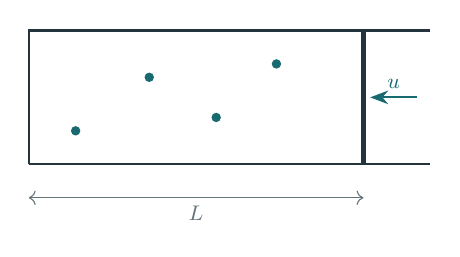
\begin{tikzpicture}[scale=.85,transform shape]

\draw[object] (0,0)--(0,2)--(6,2) (0,0)--(6,0);
\draw[object,line width=2pt] (5,0)--(5,2);
\foreach \x/\y in {.7/.5,1.8/1.3,2.8/.7,3.7/1.5}{\fill[accent] (\x,\y) circle (2pt);}
\draw[motion] (5.8,1)--(5.1,1) node[midway,above] {$u$};
\draw[axis,<->] (0,-.5)--(5,-.5) node[midway,below] {$L$};

\end{tikzpicture}
\figcaption{图综五.4\quad 一维质点只沿柱轴运动，活塞向内缓慢推进，截面积保持不变。}
\end{minipage}\end{center}

\Needspace{8\baselineskip}

\pdfbookmark[3]{题型定位}{q4-h0}

\subsection*{题型定位}

从移动壁弹性反射求速率变化，再以往返频率和容器缩短率得到速度—长度关系。平均动能给出温度，壁面冲量给出压力；随后以一维热容与绝热功说明相同的体积指数。相同质量碰撞的交换性质贯穿微观描述。

\Needspace{8\baselineskip}

\pdfbookmark[3]{知识点}{q4-h1}

\subsection*{知识点}

\begin{itemize}
\item 同质量一维弹性正碰交换速度，速度标签可连续跟踪。小球的身份改变，速率集合和平均动能保持。
\item 移动壁反射在壁系保持相对速率，回地面系后出射速率增$2u$。单次能量输入为$2muv+2mu^2$，来自活塞功。
\item 往返时间在$u/v\to0$时为$2L/v$，连续化得到$vL$；平均动能按$L^{-2}$缩放。截面积固定使体积也按$L$缩放。
\item 一维质点只有一个平动二次项，$pV=Nk_{\rm B}T$、$U=Nk_{\rm B}T/2$，故$\gamma=3$，绝热关系为$TV^2$和$pV^3$恒定。
\end{itemize}

\Needspace{8\baselineskip}

\pdfbookmark[3]{物理图像}{q4-h2}

\subsection*{物理图像}

\begin{itemize}
\item 图A分别画同质量碰撞交换速度和移动壁反射。速度标签在碰撞点交接，实际质点仍发生碰撞，等效穿行用于跟踪速度的传播。
\item 图B中活塞逐步缩短行程，每次反射增加相同的$2u$，快携带者又更频繁碰壁，累积得到统一的$1/L$速度因子。
\item 图C把微观缩放对应到温度和压力曲线。活塞外力功进入轴向平动内能；热容法只使用本题一个自由度的能量。
\end{itemize}

\Needspace{8\baselineskip}

\pdfbookmark[3]{解题入口}{q4-h3}

\subsection*{解题入口}

\begin{itemize}
\item 规定向右为正，先将入射速度换成壁系$v+u$，反射后取负，再加回壁速$-u$。两个$u$分别来自变换与反射。
\item 写$dv/dt=uv/L$和$dL/dt=-u$，消去时间后积分。碰同一个端面需要一次往返，时间取$2L/v$。
\item 先对单个速度标签求动能变化再求平均，随后用固定壁冲量算$pV$。热容比和第一定律在这个状态方程及能量定义上展开。
\end{itemize}

\Needspace{8\baselineskip}

\pdfbookmark[3]{标准解法}{q4-h4}

\subsection*{标准解法}


图综五.4把轴线向右定为正，右端活塞以速度$-u$向左推进，$u>0$，容器瞬时长度为$L$。准静态极限要求一次往返期间长度改变很小，对所跟踪速率$v$有$u\ll v$。
\begin{center}\begin{minipage}{.98\linewidth}\centering
\begin{tikzpicture}[scale=.82,transform shape]

\node at (1,2) {同质量球交换速度};
\fill (0,1) circle (3pt);\fill (2,1) circle (3pt);
\draw[motion] (0,1.3)--(1.3,1.3) node[midway,above] {$v_1$};
\draw[motion] (2,.7)--(1,.7) node[midway,below] {$v_2$};
\node at (1,-.3) {$v'_1=v_2,\quad v'_2=v_1$};
\begin{scope}[xshift=6cm]
\draw[object,line width=2pt] (2,-.5)--(2,2);
\draw[motion] (-.5,1.3)--(1.7,1.3) node[midway,above] {$v$};
\draw[motion] (1.7,.3)--(-.5,.3) node[midway,below] {$v+2u$};
\draw[motion] (2.8,1)--(2.1,1) node[above] {$-u$};
\end{scope}

\end{tikzpicture}
\figcaption{解图综五.4A\quad 速度携带者等效穿行；移动壁反射使地面系速率增加$2u$。}
\end{minipage}\end{center}
解图综五.4A中，两个同质量质点弹性正碰，动量与动能守恒：
\[
v_1+v_2=v'_1+v'_2,\qquad
v_1^2+v_2^2=v_1'^2+v_2'^2.
\]
非平凡碰撞解是$v'_1=v_2,v'_2=v_1$，即交换速度。若跟踪的不是某颗球而是某个速度的“携带者”，碰撞看起来是两条速度轨迹穿过彼此，因而可以跟踪它们在两壁间的往返。

一颗向右速率$v$的小球追上活塞，在活塞参考系中入射速度为$v+u$，弹性反射后为$-(v+u)$；变回地面系，再加活塞速度$-u$，
\[
v'_{\rm lab}=-(v+2u).
\]
因而每次与活塞相碰后速率增加$\Delta v=2u$，增加的动能由推动活塞的外力提供。
\textbf{一次碰撞怎样传递能量。} 图A中的地面系速度改变由相对速度反射与加回壁速两步组成。若入射速度为$v$，出射速度为$-(v+2u)$，单次动能增加
\[
\Delta\varepsilon=\frac m2[(v+2u)^2-v^2]
=2muv+2mu^2.
\]
向右取正，活塞对球的冲量为$\Delta p=-2m(v+u)$；恒定壁速为$-u$，碰撞功$(-u)\Delta p=2muv+2mu^2$，与球的动能增量相等。低阶每碰增加$2muv$，乘往返碰撞频率$v/(2L)$，功率为$mu v^2/L$；这也等于平均力$mv^2/L$乘推进速率$u$。微观能量增加与宏观外力做功由同一个碰撞过程联系起来。

\begin{center}\begin{minipage}{.98\linewidth}\centering
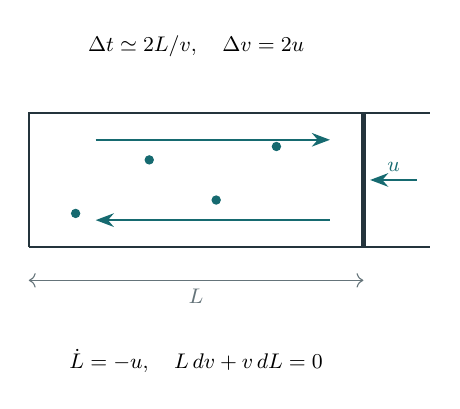
\begin{tikzpicture}[scale=.85,transform shape]

\draw[object] (0,0)--(0,2)--(6,2) (0,0)--(6,0);
\draw[object,line width=2pt] (5,0)--(5,2);
\foreach \x/\y in {.7/.5,1.8/1.3,2.8/.7,3.7/1.5}{\fill[accent] (\x,\y) circle (2pt);}
\draw[motion] (5.8,1)--(5.1,1) node[midway,above] {$u$};
\draw[axis,<->] (0,-.5)--(5,-.5) node[midway,below] {$L$};

\draw[motion] (1,1.6)--(4.5,1.6);
\draw[motion] (4.5,.4)--(1,.4);
\node at (2.5,3) {$\Delta t\simeq2L/v,\quad\Delta v=2u$};
\node at (2.5,-1.7) {$\dot L=-u,\quad L\,dv+v\,dL=0$};

\end{tikzpicture}
\figcaption{解图综五.4B\quad 两次遇同一活塞需要往返；速度与长度共同给绝热不变量。}
\end{minipage}\end{center}
解图综五.4B将连续碰撞与缓慢缩短联系起来。一个速度携带者两次碰到右端活塞之间，往返时间在一阶近似下为$\Delta t\simeq2L/v$。于是
\[
\frac{dv}{dt}\simeq\frac{2u}{2L/v}=\frac{uv}{L},
\qquad \frac{dL}{dt}=-u.
\]
消去时间，得到
\[
L\,dv+v\,dL=0,\qquad \boxed{vL=\text{常量}}.
\]
它是准静态极限的绝热不变量；连续近似采用$u/v\to0$；快速壁运动按每次精确反射和实际碰撞时刻逐次计算。

对单个携带者，$\varepsilon=mv^2/2$，有$d\varepsilon=mv\,dv$，故
\[
L\,d\varepsilon+2\varepsilon\,dL=0.
\]
因为所有速度携带者都在同一瞬时长度下缩放，对它们取平均：
\[
L\,d\overline\varepsilon+2\overline\varepsilon\,dL=0.
\]
取平均时，每个速度携带者都满足$d(v_i^2L^2)=0$，因此
\[
\langle v^2\rangle L^2
=\frac1N\sum_i v_i^2L^2=\text{常量}.
\]
这里各携带者的速率可以不同，求和只用到所有项具有相同的长度缩放因子。两球碰撞交换速度而不改变速率集合，球的身份变化与这个平均无关。

代$\overline\varepsilon=k_{\rm B}T/2$，
\[
L\,dT+2T\,dL=0,\qquad
\frac{dT}T+2\frac{dL}L=0.
\]
截面积$A$不变，$V=AL$，所以
\[
\boxed{TV^2=T_0V_0^2=\text{常量}}.
\]
容积缩小到一半，温度变为四倍。相同质量的一维碰撞只交换速度并保留速率集合，任意初始分布可保持非平衡形状；题设以平均动能定义的温度已足够上述推导。若初态为高斯平衡分布，准静态的统一速度缩放保持其形状。
\begin{center}\begin{minipage}{.98\linewidth}\centering
\begin{tikzpicture}[scale=.85,transform shape]

\draw[axis] (0,0)--(5.7,0) node[right] {$V/V_0$};
\draw[axis] (0,0)--(0,4.6) node[above] {$T/T_0$};
\draw[traj,domain=.5:2,samples=100] plot ({2.5*\x},{1/(\x*\x)});
\draw[guide] (1.25,0)--(1.25,4)--(0,4);
\node[below] at (1.25,0) {$1/2$};\node[left] at (0,4) {$4$};
\draw[guide] (2.5,0)--(2.5,1)--(0,1);
\node[below] at (2.5,0) {$1$};\node[left] at (0,1) {$1$};
\node[align=left] at (7,2) {$TV^2=\text{常量}$\\$pV^3=\text{常量}$\\$\gamma=3$};

\end{tikzpicture}
\figcaption{解图综五.4C\quad 一维平均动能温度随体积平方反比变化，对应一个轴向平动自由度和$\gamma=3$。}
\end{minipage}\end{center}
解图综五.4C再从宏观量理解同一关系。质量$m$、速率$v$的一个携带者每次碰固定壁给壁冲量$2mv$，碰壁频率$v/(2L)$，故其平均力为$mv^2/L$。对$N$个球相加，
\[
pA=\frac{Nm\langle v^2\rangle}{L},\qquad
pV=Nm\langle v^2\rangle=Nk_{\rm B}T.
\]
本题的质点没有内部转动或振动能量，能量中只有一个轴向平动平方项。若按每个二次项贡献$k_{\rm B}T/2$记数，平动贡献为1、转动和振动贡献均为0，故总数为1，得到$C_V=Nk_{\rm B}/2$。状态方程使焓$U+pV=3Nk_{\rm B}T/2$，定压热容由其温度导数得到$C_p=3Nk_{\rm B}/2$。热容比法和第一定律法正是把同一能量约定写成宏观形式。

一维质点只有一个平动自由度，
\[
U=\frac12Nk_{\rm B}T,\quad
C_V=\frac12Nk_{\rm B},\quad
C_p=C_V+Nk_{\rm B}=\frac32Nk_{\rm B}.
\]
故$\gamma=C_p/C_V=3$，可逆绝热关系$TV^{\gamma-1}=\text{常量}$再次给$TV^2=\text{常量}$。三维单原子气体的$\gamma=5/3$对应三个平动二次项，本题采用一个轴向平动项。

最后直接用第一定律。无热交换，外界对气体做功为$-p\,dV$，因此
\[
dU=-p\,dV,\qquad
\frac12Nk_{\rm B}\,dT
=-\frac{Nk_{\rm B}T}{V}\,dV.
\]
约去常数并积分，
\[
\frac{dT}T=-2\frac{dV}V,\qquad
\ln\frac T{T_0}=-2\ln\frac V{V_0}.
\]
仍得$TV^2=T_0V_0^2$；结合$pV=Nk_{\rm B}T$，还可写$pV^3=\text{常量}$。三种方法中的温度、内能和自由度约定一致。


\Needspace{8\baselineskip}

\pdfbookmark[3]{关键洞察}{q4-h5}

\subsection*{关键洞察}

\begin{itemize}
\item 同质量正碰只交换速度，任意初始分布可保持其非平衡形状。题设按平均动能定义温度，推导只需要速度统一缩放。
\item $\gamma=3$由一个平动自由度产生；三维单原子气体的三个平动二次项给另一组热容。本题的空间约束已改变能量记数。
\item 每次能量增量随$u$变小，压缩所需时间却随$1/u$增长，累积总功保持有限。慢推进同时使往返连续近似成立。
\end{itemize}

\Needspace{8\baselineskip}

\pdfbookmark[3]{易错点}{q4-h6}

\subsection*{易错点}

\begin{itemize}
\item 将壁系反射速度直接作为地面系速度会漏掉一次$-u$；图A逐步标出两个参考系。
\item 将同端相邻碰撞时间写成$L/v$会把碰撞频率加倍，进而错置升温指数。
\item 等质量正碰交换速度，两个不同速率的群体仍可存在；温度由平均动能给出，热平衡分布是额外的状态条件。
\item 套三维$\gamma=5/3$或$TV^{2/3}$会与一个轴向自由度矛盾。先按给定能量式计算热容，再使用热力学关系。
\end{itemize}

\Needspace{8\baselineskip}

\pdfbookmark[3]{课堂讲解建议}{q4-h7}

\subsection*{课堂讲解建议}

\begin{itemize}
\item 联立两球动量和动能式求速度交换，让学生沿碰撞图追踪“同一个速率”与“同一颗球”，追问只认速度标签时看到什么。答两条速度轨迹在碰撞点穿过彼此，速度标签交给另一颗球；小球的身份仍各自保留。
\item 在壁系画等长反向速度箭头，再转回地面系读出$2u$。进一步算碰撞能量增量和活塞功，把速度变化与能量传递联系起来。
\item 从$vL$依次求单球动能、平均动能、温度和压力，再以第一定律写成宏观积分。三种方法都保留同一自由度和温度定义。
\item 用变式中的匀速壁精确递推比较离散碰撞与慢壁极限，讨论一阶近似保留了哪些量；保持每次反射精确和连续描述之间的层次。
\end{itemize}

\Needspace{8\baselineskip}

\pdfbookmark[3]{变式训练}{q4-h8}

\subsection*{变式训练}

\begin{enumerate}
\Needspace{37\baselineskip}
\item \textbf{题设与求解。} 体积缓慢压到$V_0/2$，求各物理量比例。$vL$恒定且$V=AL$，故每个速率加倍，平均动能和温度增为4倍。再由$pV=Nk_{\rm B}T$得压力增为8倍。图V1画$v/v_0=V_0/V$、$T/T_0=(V_0/V)^2$，同一体积比上分别读出2和4；压力还多一个$V_0/V$因子。
\begin{center}\begin{minipage}{.98\linewidth}\centering
\begin{tikzpicture}[scale=0.72,transform shape]
\draw[axis] (0,0)--(6.2,0);\draw[axis] (0,0)--(0,3.4000000000000004);
\draw[thin,color=muted] (0.0000000,0)--(0.0000000,-.07);\node[below] at (0.0000000,-.09) {$1/2$};
\draw[thin,color=muted] (3.0000000,0)--(3.0000000,-.07);\node[below] at (3.0000000,-.09) {$1$};
\draw[thin,color=muted] (6.0000000,0)--(6.0000000,-.07);\node[below] at (6.0000000,-.09) {$1.5$};
\draw[thin,color=muted] (0,0.0000000)--(-.07,0.0000000);\node[left] at (-.09,0.0000000) {$0$};
\draw[thin,color=muted] (0,0.7619048)--(-.07,0.7619048);\node[left] at (-.09,0.7619048) {$1$};
\draw[thin,color=muted] (0,1.5238095)--(-.07,1.5238095);\node[left] at (-.09,1.5238095) {$2$};
\draw[thin,color=muted] (0,3.0476190)--(-.07,3.0476190);\node[left] at (-.09,3.0476190) {$4$};
\node[below] at (3.0,-.64) {$V/V_0$};\node[above right] at (0,3.45) {速率或温度除以初值};
\draw[traj] plot coordinates {(0.0000000,1.5238095) (0.0250000,1.5112161) (0.0500000,1.4988290) (0.0750000,1.4866434) (0.1000000,1.4746544) (0.1250000,1.4628571) (0.1500000,1.4512472) (0.1750000,1.4398200) (0.2000000,1.4285714) (0.2250000,1.4174972) (0.2500000,1.4065934) (0.2750000,1.3958561) (0.3000000,1.3852814) (0.3250000,1.3748657) (0.3500000,1.3646055) (0.3750000,1.3544974) (0.4000000,1.3445378) (0.4250000,1.3347237) (0.4500000,1.3250518) (0.4750000,1.3155190) (0.5000000,1.3061224) (0.5250000,1.2968592) (0.5500000,1.2877264) (0.5750000,1.2787213) (0.6000000,1.2698413) (0.6250000,1.2610837) (0.6500000,1.2524462) (0.6750000,1.2439261) (0.7000000,1.2355212) (0.7250000,1.2272291) (0.7500000,1.2190476) (0.7750000,1.2109745) (0.8000000,1.2030075) (0.8250000,1.1951447) (0.8500000,1.1873840) (0.8750000,1.1797235) (0.9000000,1.1721612) (0.9250000,1.1646952) (0.9500000,1.1573237) (0.9750000,1.1500449) (1.0000000,1.1428571) (1.0250000,1.1357587) (1.0500000,1.1287478) (1.0750000,1.1218230) (1.1000000,1.1149826) (1.1250000,1.1082251) (1.1500000,1.1015491) (1.1750000,1.0949530) (1.2000000,1.0884354) (1.2250000,1.0819949) (1.2500000,1.0756303) (1.2750000,1.0693400) (1.3000000,1.0631229) (1.3250000,1.0569777) (1.3500000,1.0509031) (1.3750000,1.0448980) (1.4000000,1.0389610) (1.4250000,1.0330912) (1.4500000,1.0272873) (1.4750000,1.0215483) (1.5000000,1.0158730) (1.5250000,1.0102605) (1.5500000,1.0047096) (1.5750000,0.9992194) (1.6000000,0.9937888) (1.6250000,0.9884170) (1.6500000,0.9831029) (1.6750000,0.9778457) (1.7000000,0.9726444) (1.7250000,0.9674981) (1.7500000,0.9624060) (1.7750000,0.9573672) (1.8000000,0.9523810) (1.8250000,0.9474463) (1.8500000,0.9425626) (1.8750000,0.9377289) (1.9000000,0.9329446) (1.9250000,0.9282088) (1.9500000,0.9235209) (1.9750000,0.9188801) (2.0000000,0.9142857) (2.0250000,0.9097370) (2.0500000,0.9052334) (2.0750000,0.9007741) (2.1000000,0.8963585) (2.1250000,0.8919861) (2.1500000,0.8876560) (2.1750000,0.8833678) (2.2000000,0.8791209) (2.2250000,0.8749146) (2.2500000,0.8707483) (2.2750000,0.8666215) (2.3000000,0.8625337) (2.3250000,0.8584842) (2.3500000,0.8544726) (2.3750000,0.8504983) (2.4000000,0.8465608) (2.4250000,0.8426596) (2.4500000,0.8387942) (2.4750000,0.8349641) (2.5000000,0.8311688) (2.5250000,0.8274079) (2.5500000,0.8236808) (2.5750000,0.8199872) (2.6000000,0.8163265) (2.6250000,0.8126984) (2.6500000,0.8091024) (2.6750000,0.8055381) (2.7000000,0.8020050) (2.7250000,0.7985028) (2.7500000,0.7950311) (2.7750000,0.7915894) (2.8000000,0.7881773) (2.8250000,0.7847946) (2.8500000,0.7814408) (2.8750000,0.7781155) (2.9000000,0.7748184) (2.9250000,0.7715491) (2.9500000,0.7683073) (2.9750000,0.7650926) (3.0000000,0.7619048) (3.0250000,0.7587433) (3.0500000,0.7556080) (3.0750000,0.7524985) (3.1000000,0.7494145) (3.1250000,0.7463557) (3.1500000,0.7433217) (3.1750000,0.7403123) (3.2000000,0.7373272) (3.2250000,0.7343660) (3.2500000,0.7314286) (3.2750000,0.7285145) (3.3000000,0.7256236) (3.3250000,0.7227555) (3.3500000,0.7199100) (3.3750000,0.7170868) (3.4000000,0.7142857) (3.4250000,0.7115064) (3.4500000,0.7087486) (3.4750000,0.7060121) (3.5000000,0.7032967) (3.5250000,0.7006021) (3.5500000,0.6979280) (3.5750000,0.6952743) (3.6000000,0.6926407) (3.6250000,0.6900270) (3.6500000,0.6874329) (3.6750000,0.6848582) (3.7000000,0.6823028) (3.7250000,0.6797663) (3.7500000,0.6772487) (3.7750000,0.6747496) (3.8000000,0.6722689) (3.8250000,0.6698064) (3.8500000,0.6673618) (3.8750000,0.6649351) (3.9000000,0.6625259) (3.9250000,0.6601341) (3.9500000,0.6577595) (3.9750000,0.6554019) (4.0000000,0.6530612) (4.0250000,0.6507372) (4.0500000,0.6484296) (4.0750000,0.6461383) (4.1000000,0.6438632) (4.1250000,0.6416040) (4.1500000,0.6393606) (4.1750000,0.6371329) (4.2000000,0.6349206) (4.2250000,0.6327237) (4.2500000,0.6305419) (4.2750000,0.6283751) (4.3000000,0.6262231) (4.3250000,0.6240858) (4.3500000,0.6219631) (4.3750000,0.6198547) (4.4000000,0.6177606) (4.4250000,0.6156806) (4.4500000,0.6136146) (4.4750000,0.6115624) (4.5000000,0.6095238) (4.5250000,0.6074988) (4.5500000,0.6054872) (4.5750000,0.6034889) (4.6000000,0.6015038) (4.6250000,0.5995316) (4.6500000,0.5975724) (4.6750000,0.5956259) (4.7000000,0.5936920) (4.7250000,0.5917707) (4.7500000,0.5898618) (4.7750000,0.5879651) (4.8000000,0.5860806) (4.8250000,0.5842081) (4.8500000,0.5823476) (4.8750000,0.5804989) (4.9000000,0.5786618) (4.9250000,0.5768364) (4.9500000,0.5750225) (4.9750000,0.5732199) (5.0000000,0.5714286) (5.0250000,0.5696484) (5.0500000,0.5678793) (5.0750000,0.5661212) (5.1000000,0.5643739) (5.1250000,0.5626374) (5.1500000,0.5609115) (5.1750000,0.5591962) (5.2000000,0.5574913) (5.2250000,0.5557968) (5.2500000,0.5541126) (5.2750000,0.5524385) (5.3000000,0.5507745) (5.3250000,0.5491205) (5.3500000,0.5474765) (5.3750000,0.5458422) (5.4000000,0.5442177) (5.4250000,0.5426028) (5.4500000,0.5409975) (5.4750000,0.5394016) (5.5000000,0.5378151) (5.5250000,0.5362380) (5.5500000,0.5346700) (5.5750000,0.5331112) (5.6000000,0.5315615) (5.6250000,0.5300207) (5.6500000,0.5284889) (5.6750000,0.5269658) (5.7000000,0.5254516) (5.7250000,0.5239460) (5.7500000,0.5224490) (5.7750000,0.5209605) (5.8000000,0.5194805) (5.8250000,0.5180089) (5.8500000,0.5165456) (5.8750000,0.5150905) (5.9000000,0.5136437) (5.9250000,0.5122049) (5.9500000,0.5107741) (5.9750000,0.5093514) (6.0000000,0.5079365)};
\draw[traj] (.1,-1.05)--(.7,-1.05);\node[right] at (.85,-1.05) {速率比例};\draw[dashed,thick,color=warm] plot coordinates {(0.0000000,3.0476190) (0.0250000,2.9974533) (0.0500000,2.9485161) (0.0750000,2.9007677) (0.1000000,2.8541698) (0.1250000,2.8086857) (0.1500000,2.7642803) (0.1750000,2.7209197) (0.2000000,2.6785714) (0.2250000,2.6372042) (0.2500000,2.5967878) (0.2750000,2.5572935) (0.3000000,2.5186934) (0.3250000,2.4809607) (0.3500000,2.4440696) (0.3750000,2.4079953) (0.4000000,2.3727138) (0.4250000,2.3382021) (0.4500000,2.3044378) (0.4750000,2.2713997) (0.5000000,2.2390671) (0.5250000,2.2074199) (0.5500000,2.1764389) (0.5750000,2.1461056) (0.6000000,2.1164021) (0.6250000,2.0873110) (0.6500000,2.0588156) (0.6750000,2.0308998) (0.7000000,2.0035479) (0.7250000,1.9767449) (0.7500000,1.9504762) (0.7750000,1.9247276) (0.8000000,1.8994856) (0.8250000,1.8747368) (0.8500000,1.8504686) (0.8750000,1.8266686) (0.9000000,1.8033249) (0.9250000,1.7804257) (0.9500000,1.7579600) (0.9750000,1.7359169) (1.0000000,1.7142857) (1.0250000,1.6930564) (1.0500000,1.6722190) (1.0750000,1.6517639) (1.1000000,1.6316818) (1.1250000,1.6119638) (1.1500000,1.5926010) (1.1750000,1.5735851) (1.2000000,1.5549077) (1.2250000,1.5365608) (1.2500000,1.5185368) (1.2750000,1.5008281) (1.3000000,1.4834273) (1.3250000,1.4663275) (1.3500000,1.4495215) (1.3750000,1.4330029) (1.4000000,1.4167651) (1.4250000,1.4008016) (1.4500000,1.3851065) (1.4750000,1.3696737) (1.5000000,1.3544974) (1.5250000,1.3395719) (1.5500000,1.3248917) (1.5750000,1.3104516) (1.6000000,1.2962463) (1.6250000,1.2822707) (1.6500000,1.2685199) (1.6750000,1.2549891) (1.7000000,1.2416737) (1.7250000,1.2285690) (1.7500000,1.2156708) (1.7750000,1.2029745) (1.8000000,1.1904762) (1.8250000,1.1781716) (1.8500000,1.1660568) (1.8750000,1.1541279) (1.9000000,1.1423812) (1.9250000,1.1308128) (1.9500000,1.1194193) (1.9750000,1.1081971) (2.0000000,1.0971429) (2.0250000,1.0862532) (2.0500000,1.0755248) (2.0750000,1.0649546) (2.1000000,1.0545395) (2.1250000,1.0442764) (2.1500000,1.0341624) (2.1750000,1.0241946) (2.2000000,1.0143702) (2.2250000,1.0046866) (2.2500000,0.9951409) (2.2750000,0.9857307) (2.3000000,0.9764532) (2.3250000,0.9673062) (2.3500000,0.9582871) (2.3750000,0.9493935) (2.4000000,0.9406232) (2.4250000,0.9319738) (2.4500000,0.9234432) (2.4750000,0.9150292) (2.5000000,0.9067296) (2.5250000,0.8985425) (2.5500000,0.8904658) (2.5750000,0.8824974) (2.6000000,0.8746356) (2.6250000,0.8668783) (2.6500000,0.8592238) (2.6750000,0.8516702) (2.7000000,0.8442158) (2.7250000,0.8368588) (2.7500000,0.8295976) (2.7750000,0.8224305) (2.8000000,0.8153559) (2.8250000,0.8083721) (2.8500000,0.8014777) (2.8750000,0.7946712) (2.9000000,0.7879509) (2.9250000,0.7813156) (2.9500000,0.7747637) (2.9750000,0.7682939) (3.0000000,0.7619048) (3.0250000,0.7555950) (3.0500000,0.7493633) (3.0750000,0.7432084) (3.1000000,0.7371290) (3.1250000,0.7311239) (3.1500000,0.7251919) (3.1750000,0.7193318) (3.2000000,0.7135424) (3.2250000,0.7078227) (3.2500000,0.7021714) (3.2750000,0.6965876) (3.3000000,0.6910701) (3.3250000,0.6856179) (3.3500000,0.6802299) (3.3750000,0.6749053) (3.4000000,0.6696429) (3.4250000,0.6644418) (3.4500000,0.6593010) (3.4750000,0.6542197) (3.5000000,0.6491970) (3.5250000,0.6442318) (3.5500000,0.6393234) (3.5750000,0.6344709) (3.6000000,0.6296734) (3.6250000,0.6249301) (3.6500000,0.6202402) (3.6750000,0.6156029) (3.7000000,0.6110174) (3.7250000,0.6064830) (3.7500000,0.6019988) (3.7750000,0.5975642) (3.8000000,0.5931784) (3.8250000,0.5888408) (3.8500000,0.5845505) (3.8750000,0.5803070) (3.9000000,0.5761095) (3.9250000,0.5719573) (3.9500000,0.5678499) (3.9750000,0.5637866) (4.0000000,0.5597668) (4.0250000,0.5557897) (4.0500000,0.5518550) (4.0750000,0.5479618) (4.1000000,0.5441097) (4.1250000,0.5402981) (4.1500000,0.5365264) (4.1750000,0.5327941) (4.2000000,0.5291005) (4.2250000,0.5254453) (4.2500000,0.5218278) (4.2750000,0.5182475) (4.3000000,0.5147039) (4.3250000,0.5111966) (4.3500000,0.5077250) (4.3750000,0.5042886) (4.4000000,0.5008870) (4.4250000,0.4975197) (4.4500000,0.4941862) (4.4750000,0.4908862) (4.5000000,0.4876190) (4.5250000,0.4843844) (4.5500000,0.4811819) (4.5750000,0.4780110) (4.6000000,0.4748714) (4.6250000,0.4717626) (4.6500000,0.4686842) (4.6750000,0.4656359) (4.7000000,0.4626172) (4.7250000,0.4596277) (4.7500000,0.4566672) (4.7750000,0.4537351) (4.8000000,0.4508312) (4.8250000,0.4479551) (4.8500000,0.4451064) (4.8750000,0.4422849) (4.9000000,0.4394900) (4.9250000,0.4367216) (4.9500000,0.4339792) (4.9750000,0.4312626) (5.0000000,0.4285714) (5.0250000,0.4259054) (5.0500000,0.4232641) (5.0750000,0.4206473) (5.1000000,0.4180547) (5.1250000,0.4154861) (5.1500000,0.4129410) (5.1750000,0.4104192) (5.2000000,0.4079205) (5.2250000,0.4054445) (5.2500000,0.4029909) (5.2750000,0.4005596) (5.3000000,0.3981503) (5.3250000,0.3957626) (5.3500000,0.3933963) (5.3750000,0.3910511) (5.4000000,0.3887269) (5.4250000,0.3864234) (5.4500000,0.3841402) (5.4750000,0.3818772) (5.5000000,0.3796342) (5.5250000,0.3774109) (5.5500000,0.3752070) (5.5750000,0.3730224) (5.6000000,0.3708568) (5.6250000,0.3687101) (5.6500000,0.3665819) (5.6750000,0.3644720) (5.7000000,0.3623804) (5.7250000,0.3603067) (5.7500000,0.3582507) (5.7750000,0.3562123) (5.8000000,0.3541913) (5.8250000,0.3521874) (5.8500000,0.3502004) (5.8750000,0.3482302) (5.9000000,0.3462766) (5.9250000,0.3443394) (5.9500000,0.3424184) (5.9750000,0.3405135) (6.0000000,0.3386243)};
\draw[dashed,thick,color=warm] (.1,-1.48)--(.7,-1.48);\node[right] at (.85,-1.48) {温度比例};\end{tikzpicture}
\figcaption{解图综五.4V1\quad 半体积时速率加倍、温度四倍，压力另乘体积倒数}
\end{minipage}\end{center}
\Needspace{37\baselineskip}
\item \textbf{题设与求解。} 求由$V_0$压到$V_f$所需外界功。绝热且仅有平动能，$W_{\rm on}=U_f-U_0$，于是
\[
W_{\rm on}=\frac12Nk_{\rm B}T_0
\left[\left(\frac{V_0}{V_f}\right)^2-1\right].
\]
也可将$p=p_0(V_0/V)^3$代入$-\int_{V_0}^{V_f}p\,dV$，得到相同结果。图V2画功随最终体积变化，压缩时为正，缓慢膨胀时为负；外界功与内能增量按同一符号约定相等。
\begin{center}\begin{minipage}{.98\linewidth}\centering
\begin{tikzpicture}[scale=0.72,transform shape]
\draw[axis] (0,0)--(6.2,0);\draw[axis] (0,0)--(0,3.4000000000000004);
\draw[thin,color=muted] (0.0000000,0)--(0.0000000,-.07);\node[below] at (0.0000000,-.09) {$1/2$};
\draw[thin,color=muted] (2.0000000,0)--(2.0000000,-.07);\node[below] at (2.0000000,-.09) {$1$};
\draw[thin,color=muted] (6.0000000,0)--(6.0000000,-.07);\node[below] at (6.0000000,-.09) {$2$};
\draw[thin,color=muted] (0,0.0400000)--(-.07,0.0400000);\node[left] at (-.09,0.0400000) {$-.75$};
\draw[thin,color=muted] (0,0.6400000)--(-.07,0.6400000);\node[left] at (-.09,0.6400000) {$0$};
\draw[thin,color=muted] (0,3.0400000)--(-.07,3.0400000);\node[left] at (-.09,3.0400000) {$3$};
\node[below] at (3.0,-.64) {最终体积$V/V_0$};\node[above right] at (0,3.45) {$W_{\rm on}/U_0$};
\draw[traj] plot coordinates {(0.0000000,3.0400000) (0.0250000,2.9614754) (0.0500000,2.8858061) (0.0750000,2.8128553) (0.1000000,2.7424943) (0.1250000,2.6746021) (0.1500000,2.6090644) (0.1750000,2.5457736) (0.2000000,2.4846281) (0.2250000,2.4255321) (0.2500000,2.3683951) (0.2750000,2.3131313) (0.3000000,2.2596597) (0.3250000,2.2079038) (0.3500000,2.1577909) (0.3750000,2.1092521) (0.4000000,2.0622222) (0.4250000,2.0166394) (0.4500000,1.9724448) (0.4750000,1.9295827) (0.5000000,1.8880000) (0.5250000,1.8476463) (0.5500000,1.8084737) (0.5750000,1.7704364) (0.6000000,1.7334911) (0.6250000,1.6975964) (0.6500000,1.6627127) (0.6750000,1.6288025) (0.7000000,1.5958299) (0.7250000,1.5637606) (0.7500000,1.5325620) (0.7750000,1.5022027) (0.8000000,1.4726531) (0.8250000,1.4438844) (0.8500000,1.4158695) (0.8750000,1.3885822) (0.9000000,1.3619976) (0.9250000,1.3360918) (0.9500000,1.3108417) (0.9750000,1.2862255) (1.0000000,1.2622222) (1.0250000,1.2388116) (1.0500000,1.2159742) (1.0750000,1.1936916) (1.1000000,1.1719459) (1.1250000,1.1507200) (1.1500000,1.1299975) (1.1750000,1.1097625) (1.2000000,1.0900000) (1.2250000,1.0706953) (1.2500000,1.0518343) (1.2750000,1.0334036) (1.3000000,1.0153903) (1.3250000,0.9977817) (1.3500000,0.9805658) (1.3750000,0.9637311) (1.4000000,0.9472664) (1.4250000,0.9311610) (1.4500000,0.9154043) (1.4750000,0.8999865) (1.5000000,0.8848980) (1.5250000,0.8701293) (1.5500000,0.8556715) (1.5750000,0.8415160) (1.6000000,0.8276543) (1.6250000,0.8140785) (1.6500000,0.8007806) (1.6750000,0.7877533) (1.7000000,0.7749890) (1.7250000,0.7624810) (1.7500000,0.7502222) (1.7750000,0.7382062) (1.8000000,0.7264266) (1.8250000,0.7148772) (1.8500000,0.7035520) (1.8750000,0.6924454) (1.9000000,0.6815516) (1.9250000,0.6708653) (1.9500000,0.6603813) (1.9750000,0.6500945) (2.0000000,0.6400000) (2.0250000,0.6300930) (2.0500000,0.6203688) (2.0750000,0.6108231) (2.1000000,0.6014515) (2.1250000,0.5922498) (2.1500000,0.5832138) (2.1750000,0.5743397) (2.2000000,0.5656236) (2.2250000,0.5570617) (2.2500000,0.5486505) (2.2750000,0.5403864) (2.3000000,0.5322661) (2.3250000,0.5242861) (2.3500000,0.5164434) (2.3750000,0.5087347) (2.4000000,0.5011570) (2.4250000,0.4937074) (2.4500000,0.4863830) (2.4750000,0.4791810) (2.5000000,0.4720988) (2.5250000,0.4651335) (2.5500000,0.4582828) (2.5750000,0.4515441) (2.6000000,0.4449149) (2.6250000,0.4383930) (2.6500000,0.4319760) (2.6750000,0.4256616) (2.7000000,0.4194477) (2.7250000,0.4133322) (2.7500000,0.4073130) (2.7750000,0.4013881) (2.8000000,0.3955556) (2.8250000,0.3898134) (2.8500000,0.3841598) (2.8750000,0.3785930) (2.9000000,0.3731112) (2.9250000,0.3677126) (2.9500000,0.3623957) (2.9750000,0.3571587) (3.0000000,0.3520000) (3.0250000,0.3469181) (3.0500000,0.3419116) (3.0750000,0.3369788) (3.1000000,0.3321184) (3.1250000,0.3273290) (3.1500000,0.3226091) (3.1750000,0.3179575) (3.2000000,0.3133728) (3.2250000,0.3088537) (3.2500000,0.3043991) (3.2750000,0.3000076) (3.3000000,0.2956782) (3.3250000,0.2914096) (3.3500000,0.2872006) (3.3750000,0.2830503) (3.4000000,0.2789575) (3.4250000,0.2749211) (3.4500000,0.2709402) (3.4750000,0.2670136) (3.5000000,0.2631405) (3.5250000,0.2593198) (3.5500000,0.2555507) (3.5750000,0.2518321) (3.6000000,0.2481633) (3.6250000,0.2445432) (3.6500000,0.2409711) (3.6750000,0.2374461) (3.7000000,0.2339674) (3.7250000,0.2305341) (3.7500000,0.2271456) (3.7750000,0.2238009) (3.8000000,0.2204994) (3.8250000,0.2172403) (3.8500000,0.2140229) (3.8750000,0.2108465) (3.9000000,0.2077104) (3.9250000,0.2046139) (3.9500000,0.2015564) (3.9750000,0.1985371) (4.0000000,0.1955556) (4.0250000,0.1926110) (4.0500000,0.1897029) (4.0750000,0.1868306) (4.1000000,0.1839936) (4.1250000,0.1811912) (4.1500000,0.1784229) (4.1750000,0.1756882) (4.2000000,0.1729865) (4.2250000,0.1703173) (4.2500000,0.1676800) (4.2750000,0.1650742) (4.3000000,0.1624994) (4.3250000,0.1599550) (4.3500000,0.1574406) (4.3750000,0.1549558) (4.4000000,0.1525000) (4.4250000,0.1500728) (4.4500000,0.1476738) (4.4750000,0.1453025) (4.5000000,0.1429586) (4.5250000,0.1406415) (4.5500000,0.1383509) (4.5750000,0.1360864) (4.6000000,0.1338476) (4.6250000,0.1316340) (4.6500000,0.1294454) (4.6750000,0.1272813) (4.7000000,0.1251415) (4.7250000,0.1230254) (4.7500000,0.1209328) (4.7750000,0.1188633) (4.8000000,0.1168166) (4.8250000,0.1147924) (4.8500000,0.1127902) (4.8750000,0.1108099) (4.9000000,0.1088511) (4.9250000,0.1069134) (4.9500000,0.1049966) (4.9750000,0.1031004) (5.0000000,0.1012245) (5.0250000,0.0993685) (5.0500000,0.0975323) (5.0750000,0.0957155) (5.1000000,0.0939179) (5.1250000,0.0921391) (5.1500000,0.0903790) (5.1750000,0.0886372) (5.2000000,0.0869136) (5.2250000,0.0852078) (5.2500000,0.0835196) (5.2750000,0.0818488) (5.3000000,0.0801952) (5.3250000,0.0785584) (5.3500000,0.0769383) (5.3750000,0.0753347) (5.4000000,0.0737473) (5.4250000,0.0721759) (5.4500000,0.0706202) (5.4750000,0.0690802) (5.5000000,0.0675556) (5.5250000,0.0660461) (5.5500000,0.0645516) (5.5750000,0.0630718) (5.6000000,0.0616066) (5.6250000,0.0601559) (5.6500000,0.0587193) (5.6750000,0.0572967) (5.7000000,0.0558880) (5.7250000,0.0544929) (5.7500000,0.0531113) (5.7750000,0.0517431) (5.8000000,0.0503879) (5.8250000,0.0490457) (5.8500000,0.0477163) (5.8750000,0.0463996) (5.9000000,0.0450953) (5.9250000,0.0438034) (5.9500000,0.0425236) (5.9750000,0.0412559) (6.0000000,0.0400000)};
\draw[traj] (.1,-1.05)--(.7,-1.05);\node[right] at (.85,-1.05) {外界对气体的功};\end{tikzpicture}
\figcaption{解图综五.4V2\quad 绝热压缩功为正，缓慢膨胀时气体向外做功}
\end{minipage}\end{center}
\Needspace{37\baselineskip}
\item \textbf{题设与求解。} 初态有两类速度标签，速率$v_a,v_b$，数目比例$f,1-f$，求压缩后的温度。令$\alpha=L_0/L$，两速率分别变为$\alpha v_a,\alpha v_b$，比值保持$v_a/v_b$。平均动能为$\overline\varepsilon_f=\tfrac12m\alpha^2[fv_a^2+(1-f)v_b^2]=\alpha^2\overline\varepsilon_0$，故$T_f=\alpha^2T_0$。图V3取$v_a/v_*=1,v_b/v_*=2$，画两个群体的速率随体积缩小的变化；无须将两群变成同一速率。
\begin{center}\begin{minipage}{.98\linewidth}\centering
\begin{tikzpicture}[scale=0.72,transform shape]
\draw[axis] (0,0)--(6.2,0);\draw[axis] (0,0)--(0,3.4000000000000004);
\draw[thin,color=muted] (0.0000000,0)--(0.0000000,-.07);\node[below] at (0.0000000,-.09) {$1/2$};
\draw[thin,color=muted] (3.0000000,0)--(3.0000000,-.07);\node[below] at (3.0000000,-.09) {$1$};
\draw[thin,color=muted] (6.0000000,0)--(6.0000000,-.07);\node[below] at (6.0000000,-.09) {$1.5$};
\draw[thin,color=muted] (0,0.0000000)--(-.07,0.0000000);\node[left] at (-.09,0.0000000) {$0$};
\draw[thin,color=muted] (0,0.7619048)--(-.07,0.7619048);\node[left] at (-.09,0.7619048) {$1$};
\draw[thin,color=muted] (0,1.5238095)--(-.07,1.5238095);\node[left] at (-.09,1.5238095) {$2$};
\draw[thin,color=muted] (0,3.0476190)--(-.07,3.0476190);\node[left] at (-.09,3.0476190) {$4$};
\node[below] at (3.0,-.64) {$V/V_0$};\node[above right] at (0,3.45) {速率除以参考值};
\draw[traj] plot coordinates {(0.0000000,1.5238095) (0.0250000,1.5112161) (0.0500000,1.4988290) (0.0750000,1.4866434) (0.1000000,1.4746544) (0.1250000,1.4628571) (0.1500000,1.4512472) (0.1750000,1.4398200) (0.2000000,1.4285714) (0.2250000,1.4174972) (0.2500000,1.4065934) (0.2750000,1.3958561) (0.3000000,1.3852814) (0.3250000,1.3748657) (0.3500000,1.3646055) (0.3750000,1.3544974) (0.4000000,1.3445378) (0.4250000,1.3347237) (0.4500000,1.3250518) (0.4750000,1.3155190) (0.5000000,1.3061224) (0.5250000,1.2968592) (0.5500000,1.2877264) (0.5750000,1.2787213) (0.6000000,1.2698413) (0.6250000,1.2610837) (0.6500000,1.2524462) (0.6750000,1.2439261) (0.7000000,1.2355212) (0.7250000,1.2272291) (0.7500000,1.2190476) (0.7750000,1.2109745) (0.8000000,1.2030075) (0.8250000,1.1951447) (0.8500000,1.1873840) (0.8750000,1.1797235) (0.9000000,1.1721612) (0.9250000,1.1646952) (0.9500000,1.1573237) (0.9750000,1.1500449) (1.0000000,1.1428571) (1.0250000,1.1357587) (1.0500000,1.1287478) (1.0750000,1.1218230) (1.1000000,1.1149826) (1.1250000,1.1082251) (1.1500000,1.1015491) (1.1750000,1.0949530) (1.2000000,1.0884354) (1.2250000,1.0819949) (1.2500000,1.0756303) (1.2750000,1.0693400) (1.3000000,1.0631229) (1.3250000,1.0569777) (1.3500000,1.0509031) (1.3750000,1.0448980) (1.4000000,1.0389610) (1.4250000,1.0330912) (1.4500000,1.0272873) (1.4750000,1.0215483) (1.5000000,1.0158730) (1.5250000,1.0102605) (1.5500000,1.0047096) (1.5750000,0.9992194) (1.6000000,0.9937888) (1.6250000,0.9884170) (1.6500000,0.9831029) (1.6750000,0.9778457) (1.7000000,0.9726444) (1.7250000,0.9674981) (1.7500000,0.9624060) (1.7750000,0.9573672) (1.8000000,0.9523810) (1.8250000,0.9474463) (1.8500000,0.9425626) (1.8750000,0.9377289) (1.9000000,0.9329446) (1.9250000,0.9282088) (1.9500000,0.9235209) (1.9750000,0.9188801) (2.0000000,0.9142857) (2.0250000,0.9097370) (2.0500000,0.9052334) (2.0750000,0.9007741) (2.1000000,0.8963585) (2.1250000,0.8919861) (2.1500000,0.8876560) (2.1750000,0.8833678) (2.2000000,0.8791209) (2.2250000,0.8749146) (2.2500000,0.8707483) (2.2750000,0.8666215) (2.3000000,0.8625337) (2.3250000,0.8584842) (2.3500000,0.8544726) (2.3750000,0.8504983) (2.4000000,0.8465608) (2.4250000,0.8426596) (2.4500000,0.8387942) (2.4750000,0.8349641) (2.5000000,0.8311688) (2.5250000,0.8274079) (2.5500000,0.8236808) (2.5750000,0.8199872) (2.6000000,0.8163265) (2.6250000,0.8126984) (2.6500000,0.8091024) (2.6750000,0.8055381) (2.7000000,0.8020050) (2.7250000,0.7985028) (2.7500000,0.7950311) (2.7750000,0.7915894) (2.8000000,0.7881773) (2.8250000,0.7847946) (2.8500000,0.7814408) (2.8750000,0.7781155) (2.9000000,0.7748184) (2.9250000,0.7715491) (2.9500000,0.7683073) (2.9750000,0.7650926) (3.0000000,0.7619048) (3.0250000,0.7587433) (3.0500000,0.7556080) (3.0750000,0.7524985) (3.1000000,0.7494145) (3.1250000,0.7463557) (3.1500000,0.7433217) (3.1750000,0.7403123) (3.2000000,0.7373272) (3.2250000,0.7343660) (3.2500000,0.7314286) (3.2750000,0.7285145) (3.3000000,0.7256236) (3.3250000,0.7227555) (3.3500000,0.7199100) (3.3750000,0.7170868) (3.4000000,0.7142857) (3.4250000,0.7115064) (3.4500000,0.7087486) (3.4750000,0.7060121) (3.5000000,0.7032967) (3.5250000,0.7006021) (3.5500000,0.6979280) (3.5750000,0.6952743) (3.6000000,0.6926407) (3.6250000,0.6900270) (3.6500000,0.6874329) (3.6750000,0.6848582) (3.7000000,0.6823028) (3.7250000,0.6797663) (3.7500000,0.6772487) (3.7750000,0.6747496) (3.8000000,0.6722689) (3.8250000,0.6698064) (3.8500000,0.6673618) (3.8750000,0.6649351) (3.9000000,0.6625259) (3.9250000,0.6601341) (3.9500000,0.6577595) (3.9750000,0.6554019) (4.0000000,0.6530612) (4.0250000,0.6507372) (4.0500000,0.6484296) (4.0750000,0.6461383) (4.1000000,0.6438632) (4.1250000,0.6416040) (4.1500000,0.6393606) (4.1750000,0.6371329) (4.2000000,0.6349206) (4.2250000,0.6327237) (4.2500000,0.6305419) (4.2750000,0.6283751) (4.3000000,0.6262231) (4.3250000,0.6240858) (4.3500000,0.6219631) (4.3750000,0.6198547) (4.4000000,0.6177606) (4.4250000,0.6156806) (4.4500000,0.6136146) (4.4750000,0.6115624) (4.5000000,0.6095238) (4.5250000,0.6074988) (4.5500000,0.6054872) (4.5750000,0.6034889) (4.6000000,0.6015038) (4.6250000,0.5995316) (4.6500000,0.5975724) (4.6750000,0.5956259) (4.7000000,0.5936920) (4.7250000,0.5917707) (4.7500000,0.5898618) (4.7750000,0.5879651) (4.8000000,0.5860806) (4.8250000,0.5842081) (4.8500000,0.5823476) (4.8750000,0.5804989) (4.9000000,0.5786618) (4.9250000,0.5768364) (4.9500000,0.5750225) (4.9750000,0.5732199) (5.0000000,0.5714286) (5.0250000,0.5696484) (5.0500000,0.5678793) (5.0750000,0.5661212) (5.1000000,0.5643739) (5.1250000,0.5626374) (5.1500000,0.5609115) (5.1750000,0.5591962) (5.2000000,0.5574913) (5.2250000,0.5557968) (5.2500000,0.5541126) (5.2750000,0.5524385) (5.3000000,0.5507745) (5.3250000,0.5491205) (5.3500000,0.5474765) (5.3750000,0.5458422) (5.4000000,0.5442177) (5.4250000,0.5426028) (5.4500000,0.5409975) (5.4750000,0.5394016) (5.5000000,0.5378151) (5.5250000,0.5362380) (5.5500000,0.5346700) (5.5750000,0.5331112) (5.6000000,0.5315615) (5.6250000,0.5300207) (5.6500000,0.5284889) (5.6750000,0.5269658) (5.7000000,0.5254516) (5.7250000,0.5239460) (5.7500000,0.5224490) (5.7750000,0.5209605) (5.8000000,0.5194805) (5.8250000,0.5180089) (5.8500000,0.5165456) (5.8750000,0.5150905) (5.9000000,0.5136437) (5.9250000,0.5122049) (5.9500000,0.5107741) (5.9750000,0.5093514) (6.0000000,0.5079365)};
\draw[traj] (.1,-1.05)--(.7,-1.05);\node[right] at (.85,-1.05) {初始速率为1的一群};\draw[dashed,thick,color=warm] plot coordinates {(0.0000000,3.0476190) (0.0250000,3.0224321) (0.0500000,2.9976581) (0.0750000,2.9732869) (0.1000000,2.9493088) (0.1250000,2.9257143) (0.1500000,2.9024943) (0.1750000,2.8796400) (0.2000000,2.8571429) (0.2250000,2.8349945) (0.2500000,2.8131868) (0.2750000,2.7917121) (0.3000000,2.7705628) (0.3250000,2.7497315) (0.3500000,2.7292111) (0.3750000,2.7089947) (0.4000000,2.6890756) (0.4250000,2.6694473) (0.4500000,2.6501035) (0.4750000,2.6310380) (0.5000000,2.6122449) (0.5250000,2.5937183) (0.5500000,2.5754527) (0.5750000,2.5574426) (0.6000000,2.5396825) (0.6250000,2.5221675) (0.6500000,2.5048924) (0.6750000,2.4878523) (0.7000000,2.4710425) (0.7250000,2.4544583) (0.7500000,2.4380952) (0.7750000,2.4219489) (0.8000000,2.4060150) (0.8250000,2.3902894) (0.8500000,2.3747681) (0.8750000,2.3594470) (0.9000000,2.3443223) (0.9250000,2.3293904) (0.9500000,2.3146474) (0.9750000,2.3000898) (1.0000000,2.2857143) (1.0250000,2.2715173) (1.0500000,2.2574956) (1.0750000,2.2436459) (1.1000000,2.2299652) (1.1250000,2.2164502) (1.1500000,2.2030981) (1.1750000,2.1899059) (1.2000000,2.1768707) (1.2250000,2.1639899) (1.2500000,2.1512605) (1.2750000,2.1386800) (1.3000000,2.1262458) (1.3250000,2.1139554) (1.3500000,2.1018062) (1.3750000,2.0897959) (1.4000000,2.0779221) (1.4250000,2.0661824) (1.4500000,2.0545746) (1.4750000,2.0430966) (1.5000000,2.0317460) (1.5250000,2.0205209) (1.5500000,2.0094192) (1.5750000,1.9984387) (1.6000000,1.9875776) (1.6250000,1.9768340) (1.6500000,1.9662058) (1.6750000,1.9556914) (1.7000000,1.9452888) (1.7250000,1.9349962) (1.7500000,1.9248120) (1.7750000,1.9147345) (1.8000000,1.9047619) (1.8250000,1.8948927) (1.8500000,1.8851252) (1.8750000,1.8754579) (1.9000000,1.8658892) (1.9250000,1.8564177) (1.9500000,1.8470418) (1.9750000,1.8377602) (2.0000000,1.8285714) (2.0250000,1.8194741) (2.0500000,1.8104668) (2.0750000,1.8015482) (2.1000000,1.7927171) (2.1250000,1.7839721) (2.1500000,1.7753121) (2.1750000,1.7667357) (2.2000000,1.7582418) (2.2250000,1.7498291) (2.2500000,1.7414966) (2.2750000,1.7332431) (2.3000000,1.7250674) (2.3250000,1.7169685) (2.3500000,1.7089453) (2.3750000,1.7009967) (2.4000000,1.6931217) (2.4250000,1.6853193) (2.4500000,1.6775885) (2.4750000,1.6699282) (2.5000000,1.6623377) (2.5250000,1.6548158) (2.5500000,1.6473616) (2.5750000,1.6399744) (2.6000000,1.6326531) (2.6250000,1.6253968) (2.6500000,1.6182048) (2.6750000,1.6110761) (2.7000000,1.6040100) (2.7250000,1.5970056) (2.7500000,1.5900621) (2.7750000,1.5831787) (2.8000000,1.5763547) (2.8250000,1.5695892) (2.8500000,1.5628816) (2.8750000,1.5562310) (2.9000000,1.5496368) (2.9250000,1.5430983) (2.9500000,1.5366146) (2.9750000,1.5301853) (3.0000000,1.5238095) (3.0250000,1.5174867) (3.0500000,1.5112161) (3.0750000,1.5049971) (3.1000000,1.4988290) (3.1250000,1.4927114) (3.1500000,1.4866434) (3.1750000,1.4806246) (3.2000000,1.4746544) (3.2250000,1.4687321) (3.2500000,1.4628571) (3.2750000,1.4570290) (3.3000000,1.4512472) (3.3250000,1.4455110) (3.3500000,1.4398200) (3.3750000,1.4341737) (3.4000000,1.4285714) (3.4250000,1.4230128) (3.4500000,1.4174972) (3.4750000,1.4120243) (3.5000000,1.4065934) (3.5250000,1.4012042) (3.5500000,1.3958561) (3.5750000,1.3905486) (3.6000000,1.3852814) (3.6250000,1.3800539) (3.6500000,1.3748657) (3.6750000,1.3697164) (3.7000000,1.3646055) (3.7250000,1.3595327) (3.7500000,1.3544974) (3.7750000,1.3494992) (3.8000000,1.3445378) (3.8250000,1.3396128) (3.8500000,1.3347237) (3.8750000,1.3298701) (3.9000000,1.3250518) (3.9250000,1.3202682) (3.9500000,1.3155190) (3.9750000,1.3108039) (4.0000000,1.3061224) (4.0250000,1.3014743) (4.0500000,1.2968592) (4.0750000,1.2922766) (4.1000000,1.2877264) (4.1250000,1.2832080) (4.1500000,1.2787213) (4.1750000,1.2742658) (4.2000000,1.2698413) (4.2250000,1.2654474) (4.2500000,1.2610837) (4.2750000,1.2567501) (4.3000000,1.2524462) (4.3250000,1.2481716) (4.3500000,1.2439261) (4.3750000,1.2397094) (4.4000000,1.2355212) (4.4250000,1.2313612) (4.4500000,1.2272291) (4.4750000,1.2231247) (4.5000000,1.2190476) (4.5250000,1.2149976) (4.5500000,1.2109745) (4.5750000,1.2069778) (4.6000000,1.2030075) (4.6250000,1.1990632) (4.6500000,1.1951447) (4.6750000,1.1912517) (4.7000000,1.1873840) (4.7250000,1.1835414) (4.7500000,1.1797235) (4.7750000,1.1759302) (4.8000000,1.1721612) (4.8250000,1.1684162) (4.8500000,1.1646952) (4.8750000,1.1609977) (4.9000000,1.1573237) (4.9250000,1.1536728) (4.9500000,1.1500449) (4.9750000,1.1464398) (5.0000000,1.1428571) (5.0250000,1.1392968) (5.0500000,1.1357587) (5.0750000,1.1322424) (5.1000000,1.1287478) (5.1250000,1.1252747) (5.1500000,1.1218230) (5.1750000,1.1183923) (5.2000000,1.1149826) (5.2250000,1.1115936) (5.2500000,1.1082251) (5.2750000,1.1048770) (5.3000000,1.1015491) (5.3250000,1.0982411) (5.3500000,1.0949530) (5.3750000,1.0916844) (5.4000000,1.0884354) (5.4250000,1.0852056) (5.4500000,1.0819949) (5.4750000,1.0788032) (5.5000000,1.0756303) (5.5250000,1.0724759) (5.5500000,1.0693400) (5.5750000,1.0662224) (5.6000000,1.0631229) (5.6250000,1.0600414) (5.6500000,1.0569777) (5.6750000,1.0539317) (5.7000000,1.0509031) (5.7250000,1.0478919) (5.7500000,1.0448980) (5.7750000,1.0419210) (5.8000000,1.0389610) (5.8250000,1.0360178) (5.8500000,1.0330912) (5.8750000,1.0301811) (5.9000000,1.0272873) (5.9250000,1.0244098) (5.9500000,1.0215483) (5.9750000,1.0187027) (6.0000000,1.0158730)};
\draw[dashed,thick,color=warm] (.1,-1.48)--(.7,-1.48);\node[right] at (.85,-1.48) {初始速率为2的一群};\end{tikzpicture}
\figcaption{解图综五.4V3\quad 两群速率按相同比例增长，速率比始终为2}
\end{minipage}\end{center}
\Needspace{37\baselineskip}
\item \textbf{题设与求解。} 推广到$d$维平动理想气体的可逆绝热过程。热平衡下$U=dNk_{\rm B}T/2$，而$pV=Nk_{\rm B}T$，第一定律给$(d/2)dT/T=-dV/V$，积分为$TV^{2/d}$恒定。热容比$\gamma=1+2/d$。图V4比较$d=1$和$d=3$的温度曲线，前者指数2，后者指数$2/3$；两种模型的体积与自由度定义各自一致。
\begin{center}\begin{minipage}{.98\linewidth}\centering
\begin{tikzpicture}[scale=0.72,transform shape]
\draw[axis] (0,0)--(6.2,0);\draw[axis] (0,0)--(0,3.4000000000000004);
\draw[thin,color=muted] (0.0000000,0)--(0.0000000,-.07);\node[below] at (0.0000000,-.09) {$1/2$};
\draw[thin,color=muted] (2.0000000,0)--(2.0000000,-.07);\node[below] at (2.0000000,-.09) {$1$};
\draw[thin,color=muted] (6.0000000,0)--(6.0000000,-.07);\node[below] at (6.0000000,-.09) {$2$};
\draw[thin,color=muted] (0,0.0000000)--(-.07,0.0000000);\node[left] at (-.09,0.0000000) {$0$};
\draw[thin,color=muted] (0,0.7619048)--(-.07,0.7619048);\node[left] at (-.09,0.7619048) {$1$};
\draw[thin,color=muted] (0,1.5238095)--(-.07,1.5238095);\node[left] at (-.09,1.5238095) {$2$};
\draw[thin,color=muted] (0,3.0476190)--(-.07,3.0476190);\node[left] at (-.09,3.0476190) {$4$};
\node[below] at (3.0,-.64) {$V/V_0$};\node[above right] at (0,3.45) {$T/T_0$};
\draw[traj] plot coordinates {(0.0000000,3.0476190) (0.0250000,2.9728337) (0.0500000,2.9007677) (0.0750000,2.8312907) (0.1000000,2.7642803) (0.1250000,2.6996210) (0.1500000,2.6372042) (0.1750000,2.5769272) (0.2000000,2.5186934) (0.2250000,2.4624116) (0.2500000,2.4079953) (0.2750000,2.3553631) (0.3000000,2.3044378) (0.3250000,2.2551465) (0.3500000,2.2074199) (0.3750000,2.1611925) (0.4000000,2.1164021) (0.4250000,2.0729899) (0.4500000,2.0308998) (0.4750000,1.9900788) (0.5000000,1.9504762) (0.5250000,1.9120441) (0.5500000,1.8747368) (0.5750000,1.8385109) (0.6000000,1.8033249) (0.6250000,1.7691394) (0.6500000,1.7359169) (0.6750000,1.7036214) (0.7000000,1.6722190) (0.7250000,1.6416768) (0.7500000,1.6119638) (0.7750000,1.5830502) (0.8000000,1.5549077) (0.8250000,1.5275090) (0.8500000,1.5008281) (0.8750000,1.4748402) (0.9000000,1.4495215) (0.9250000,1.4248493) (0.9500000,1.4008016) (0.9750000,1.3773577) (1.0000000,1.3544974) (1.0250000,1.3322015) (1.0500000,1.3104516) (1.0750000,1.2892301) (1.1000000,1.2685199) (1.1250000,1.2483048) (1.1500000,1.2285690) (1.1750000,1.2092977) (1.2000000,1.1904762) (1.2250000,1.1720907) (1.2500000,1.1541279) (1.2750000,1.1365749) (1.3000000,1.1194193) (1.3250000,1.1026492) (1.3500000,1.0862532) (1.3750000,1.0702201) (1.4000000,1.0545395) (1.4250000,1.0392009) (1.4500000,1.0241946) (1.4750000,1.0095110) (1.5000000,0.9951409) (1.5250000,0.9810755) (1.5500000,0.9673062) (1.5750000,0.9538247) (1.6000000,0.9406232) (1.6250000,0.9276938) (1.6500000,0.9150292) (1.6750000,0.9026221) (1.7000000,0.8904658) (1.7250000,0.8785533) (1.7500000,0.8668783) (1.7750000,0.8554345) (1.8000000,0.8442158) (1.8250000,0.8332164) (1.8500000,0.8224305) (1.8750000,0.8118527) (1.9000000,0.8014777) (1.9250000,0.7913003) (1.9500000,0.7813156) (1.9750000,0.7715186) (2.0000000,0.7619048) (2.0250000,0.7524695) (2.0500000,0.7432084) (2.0750000,0.7341173) (2.1000000,0.7251919) (2.1250000,0.7164284) (2.1500000,0.7078227) (2.1750000,0.6993711) (2.2000000,0.6910701) (2.2250000,0.6829159) (2.2500000,0.6749053) (2.2750000,0.6670347) (2.3000000,0.6593010) (2.3250000,0.6517011) (2.3500000,0.6442318) (2.3750000,0.6368902) (2.4000000,0.6296734) (2.4250000,0.6225785) (2.4500000,0.6156029) (2.4750000,0.6087439) (2.5000000,0.6019988) (2.5250000,0.5953653) (2.5500000,0.5888408) (2.5750000,0.5824229) (2.6000000,0.5761095) (2.6250000,0.5698981) (2.6500000,0.5637866) (2.6750000,0.5577729) (2.7000000,0.5518550) (2.7250000,0.5460307) (2.7500000,0.5402981) (2.7750000,0.5346554) (2.8000000,0.5291005) (2.8250000,0.5236318) (2.8500000,0.5182475) (2.8750000,0.5129457) (2.9000000,0.5077250) (2.9250000,0.5025835) (2.9500000,0.4975197) (2.9750000,0.4925321) (3.0000000,0.4876190) (3.0250000,0.4827792) (3.0500000,0.4780110) (3.0750000,0.4733132) (3.1000000,0.4686842) (3.1250000,0.4641228) (3.1500000,0.4596277) (3.1750000,0.4551976) (3.2000000,0.4508312) (3.2250000,0.4465274) (3.2500000,0.4422849) (3.2750000,0.4381025) (3.3000000,0.4339792) (3.3250000,0.4299139) (3.3500000,0.4259054) (3.3750000,0.4219527) (3.4000000,0.4180547) (3.4250000,0.4142106) (3.4500000,0.4104192) (3.4750000,0.4066796) (3.5000000,0.4029909) (3.5250000,0.3993522) (3.5500000,0.3957626) (3.5750000,0.3922211) (3.6000000,0.3887269) (3.6250000,0.3852792) (3.6500000,0.3818772) (3.6750000,0.3785201) (3.7000000,0.3752070) (3.7250000,0.3719373) (3.7500000,0.3687101) (3.7750000,0.3655247) (3.8000000,0.3623804) (3.8250000,0.3592765) (3.8500000,0.3562123) (3.8750000,0.3531872) (3.9000000,0.3502004) (3.9250000,0.3472514) (3.9500000,0.3443394) (3.9750000,0.3414639) (4.0000000,0.3386243) (4.0250000,0.3358200) (4.0500000,0.3330504) (4.0750000,0.3303149) (4.1000000,0.3276129) (4.1250000,0.3249440) (4.1500000,0.3223075) (4.1750000,0.3197030) (4.2000000,0.3171300) (4.2250000,0.3145879) (4.2500000,0.3120762) (4.2750000,0.3095945) (4.3000000,0.3071423) (4.3250000,0.3047191) (4.3500000,0.3023244) (4.3750000,0.2999579) (4.4000000,0.2976190) (4.4250000,0.2953075) (4.4500000,0.2930227) (4.4750000,0.2907643) (4.5000000,0.2885320) (4.5250000,0.2863252) (4.5500000,0.2841437) (4.5750000,0.2819870) (4.6000000,0.2798548) (4.6250000,0.2777467) (4.6500000,0.2756623) (4.6750000,0.2736013) (4.7000000,0.2715633) (4.7250000,0.2695480) (4.7500000,0.2675550) (4.7750000,0.2655841) (4.8000000,0.2636349) (4.8250000,0.2617070) (4.8500000,0.2598002) (4.8750000,0.2579142) (4.9000000,0.2560486) (4.9250000,0.2542033) (4.9500000,0.2523777) (4.9750000,0.2505718) (5.0000000,0.2487852) (5.0250000,0.2470177) (5.0500000,0.2452689) (5.0750000,0.2435386) (5.1000000,0.2418265) (5.1250000,0.2401325) (5.1500000,0.2384562) (5.1750000,0.2367974) (5.2000000,0.2351558) (5.2250000,0.2335312) (5.2500000,0.2319234) (5.2750000,0.2303322) (5.3000000,0.2287573) (5.3250000,0.2271985) (5.3500000,0.2256555) (5.3750000,0.2241283) (5.4000000,0.2226164) (5.4250000,0.2211199) (5.4500000,0.2196383) (5.4750000,0.2181716) (5.5000000,0.2167196) (5.5250000,0.2152820) (5.5500000,0.2138586) (5.5750000,0.2124493) (5.6000000,0.2110540) (5.6250000,0.2096723) (5.6500000,0.2083041) (5.6750000,0.2069493) (5.7000000,0.2056076) (5.7250000,0.2042790) (5.7500000,0.2029632) (5.7750000,0.2016601) (5.8000000,0.2003694) (5.8250000,0.1990912) (5.8500000,0.1978251) (5.8750000,0.1965710) (5.9000000,0.1953289) (5.9250000,0.1940985) (5.9500000,0.1928797) (5.9750000,0.1916723) (6.0000000,0.1904762)};
\draw[traj] (.1,-1.05)--(.7,-1.05);\node[right] at (.85,-1.05) {一维平动};\draw[dashed,thick,color=warm] plot coordinates {(0.0000000,1.2094484) (0.0250000,1.1994735) (0.0500000,1.1897018) (0.0750000,1.1801266) (0.1000000,1.1707419) (0.1250000,1.1615415) (0.1500000,1.1525197) (0.1750000,1.1436712) (0.2000000,1.1349905) (0.2250000,1.1264727) (0.2500000,1.1181129) (0.2750000,1.1099066) (0.3000000,1.1018491) (0.3250000,1.0939363) (0.3500000,1.0861641) (0.3750000,1.0785285) (0.4000000,1.0710256) (0.4250000,1.0636519) (0.4500000,1.0564038) (0.4750000,1.0492780) (0.5000000,1.0422711) (0.5250000,1.0353800) (0.5500000,1.0286017) (0.5750000,1.0219332) (0.6000000,1.0153718) (0.6250000,1.0089148) (0.6500000,1.0025594) (0.6750000,0.9963031) (0.7000000,0.9901436) (0.7250000,0.9840784) (0.7500000,0.9781052) (0.7750000,0.9722218) (0.8000000,0.9664261) (0.8250000,0.9607161) (0.8500000,0.9550896) (0.8750000,0.9495448) (0.9000000,0.9440798) (0.9250000,0.9386927) (0.9500000,0.9333818) (0.9750000,0.9281454) (1.0000000,0.9229819) (1.0250000,0.9178896) (1.0500000,0.9128669) (1.0750000,0.9079124) (1.1000000,0.9030245) (1.1250000,0.8982020) (1.1500000,0.8934433) (1.1750000,0.8887471) (1.2000000,0.8841122) (1.2250000,0.8795372) (1.2500000,0.8750209) (1.2750000,0.8705622) (1.3000000,0.8661599) (1.3250000,0.8618128) (1.3500000,0.8575198) (1.3750000,0.8532799) (1.4000000,0.8490920) (1.4250000,0.8449551) (1.4500000,0.8408682) (1.4750000,0.8368305) (1.5000000,0.8328408) (1.5250000,0.8288983) (1.5500000,0.8250022) (1.5750000,0.8211516) (1.6000000,0.8173455) (1.6250000,0.8135833) (1.6500000,0.8098640) (1.6750000,0.8061870) (1.7000000,0.8025514) (1.7250000,0.7989566) (1.7500000,0.7954017) (1.7750000,0.7918861) (1.8000000,0.7884091) (1.8250000,0.7849700) (1.8500000,0.7815682) (1.8750000,0.7782030) (1.9000000,0.7748737) (1.9250000,0.7715799) (1.9500000,0.7683208) (1.9750000,0.7650960) (2.0000000,0.7619048) (2.0250000,0.7587466) (2.0500000,0.7556210) (2.0750000,0.7525273) (2.1000000,0.7494652) (2.1250000,0.7464339) (2.1500000,0.7434332) (2.1750000,0.7404624) (2.2000000,0.7375212) (2.2250000,0.7346089) (2.2500000,0.7317253) (2.2750000,0.7288698) (2.3000000,0.7260419) (2.3250000,0.7232414) (2.3500000,0.7204677) (2.3750000,0.7177204) (2.4000000,0.7149992) (2.4250000,0.7123036) (2.4500000,0.7096333) (2.4750000,0.7069879) (2.5000000,0.7043670) (2.5250000,0.7017703) (2.5500000,0.6991973) (2.5750000,0.6966478) (2.6000000,0.6941214) (2.6250000,0.6916178) (2.6500000,0.6891367) (2.6750000,0.6866777) (2.7000000,0.6842405) (2.7250000,0.6818248) (2.7500000,0.6794303) (2.7750000,0.6770568) (2.8000000,0.6747039) (2.8250000,0.6723713) (2.8500000,0.6700587) (2.8750000,0.6677659) (2.9000000,0.6654927) (2.9250000,0.6632387) (2.9500000,0.6610037) (2.9750000,0.6587874) (3.0000000,0.6565896) (3.0250000,0.6544101) (3.0500000,0.6522485) (3.0750000,0.6501047) (3.1000000,0.6479785) (3.1250000,0.6458695) (3.1500000,0.6437776) (3.1750000,0.6417026) (3.2000000,0.6396442) (3.2250000,0.6376022) (3.2500000,0.6355765) (3.2750000,0.6335667) (3.3000000,0.6315728) (3.3250000,0.6295945) (3.3500000,0.6276316) (3.3750000,0.6256840) (3.4000000,0.6237514) (3.4250000,0.6218336) (3.4500000,0.6199305) (3.4750000,0.6180419) (3.5000000,0.6161676) (3.5250000,0.6143075) (3.5500000,0.6124614) (3.5750000,0.6106290) (3.6000000,0.6088103) (3.6250000,0.6070051) (3.6500000,0.6052132) (3.6750000,0.6034345) (3.7000000,0.6016687) (3.7250000,0.5999159) (3.7500000,0.5981757) (3.7750000,0.5964481) (3.8000000,0.5947330) (3.8250000,0.5930301) (3.8500000,0.5913393) (3.8750000,0.5896606) (3.9000000,0.5879937) (3.9250000,0.5863385) (3.9500000,0.5846950) (3.9750000,0.5830629) (4.0000000,0.5814422) (4.0250000,0.5798326) (4.0500000,0.5782342) (4.0750000,0.5766467) (4.1000000,0.5750701) (4.1250000,0.5735042) (4.1500000,0.5719490) (4.1750000,0.5704042) (4.2000000,0.5688698) (4.2250000,0.5673457) (4.2500000,0.5658318) (4.2750000,0.5643279) (4.3000000,0.5628340) (4.3250000,0.5613499) (4.3500000,0.5598756) (4.3750000,0.5584109) (4.4000000,0.5569558) (4.4250000,0.5555101) (4.4500000,0.5540737) (4.4750000,0.5526466) (4.5000000,0.5512286) (4.5250000,0.5498198) (4.5500000,0.5484198) (4.5750000,0.5470288) (4.6000000,0.5456465) (4.6250000,0.5442730) (4.6500000,0.5429080) (4.6750000,0.5415516) (4.7000000,0.5402036) (4.7250000,0.5388640) (4.7500000,0.5375326) (4.7750000,0.5362095) (4.8000000,0.5348944) (4.8250000,0.5335874) (4.8500000,0.5322884) (4.8750000,0.5309972) (4.9000000,0.5297138) (4.9250000,0.5284382) (4.9500000,0.5271702) (4.9750000,0.5259097) (5.0000000,0.5246568) (5.0250000,0.5234113) (5.0500000,0.5221732) (5.0750000,0.5209424) (5.1000000,0.5197188) (5.1250000,0.5185024) (5.1500000,0.5172931) (5.1750000,0.5160908) (5.2000000,0.5148954) (5.2250000,0.5137070) (5.2500000,0.5125253) (5.2750000,0.5113505) (5.3000000,0.5101824) (5.3250000,0.5090209) (5.3500000,0.5078660) (5.3750000,0.5067176) (5.4000000,0.5055757) (5.4250000,0.5044402) (5.4500000,0.5033111) (5.4750000,0.5021883) (5.5000000,0.5010717) (5.5250000,0.4999613) (5.5500000,0.4988570) (5.5750000,0.4977588) (5.6000000,0.4966666) (5.6250000,0.4955804) (5.6500000,0.4945001) (5.6750000,0.4934257) (5.7000000,0.4923571) (5.7250000,0.4912943) (5.7500000,0.4902371) (5.7750000,0.4891857) (5.8000000,0.4881399) (5.8250000,0.4870996) (5.8500000,0.4860649) (5.8750000,0.4850356) (5.9000000,0.4840118) (5.9250000,0.4829934) (5.9500000,0.4819803) (5.9750000,0.4809725) (6.0000000,0.4799699)};
\draw[dashed,thick,color=warm] (.1,-1.48)--(.7,-1.48);\node[right] at (.85,-1.48) {三维平动};\end{tikzpicture}
\figcaption{解图综五.4V4\quad 平动自由度改变热容，体积指数随之改变}
\end{minipage}\end{center}
\Needspace{37\baselineskip}
\item \textbf{题设与求解。} 右壁以恒速$-u$推进，记第$n$次反射后的出射速率$v_n$、当时长度$L_n$，求精确离散关系。到固定左壁的时间为$L_n/v_n$，随后追上右壁的时间为$L_n(v_n-u)/[v_n(v_n+u)]$，故总间隔$2L_n/(v_n+u)$。于是
\[
L_{n+1}=L_n\frac{v_n-u}{v_n+u},\qquad
v_{n+1}=v_n+2u,\qquad
(v_{n+1}-u)L_{n+1}=(v_n-u)L_n.
\]
图V5画$v_nL_n$与$(v_n-u)L_n$，后者在匀速壁离散碰撞时精确恒定。$u/v_n\to0$时两者相近，得到主解的准静态$vL$关系。
\begin{center}\begin{minipage}{.98\linewidth}\centering
\begin{tikzpicture}[scale=0.72,transform shape]
\draw[axis] (0,0)--(6.2,0);\draw[axis] (0,0)--(0,3.4000000000000004);
\draw[thin,color=muted] (0.0000000,0)--(0.0000000,-.07);\node[below] at (0.0000000,-.09) {$0$};
\draw[thin,color=muted] (3.0000000,0)--(3.0000000,-.07);\node[below] at (3.0000000,-.09) {$6$};
\draw[thin,color=muted] (6.0000000,0)--(6.0000000,-.07);\node[below] at (6.0000000,-.09) {$12$};
\draw[thin,color=muted] (0,0.4923077)--(-.07,0.4923077);\node[left] at (-.09,0.4923077) {$.95$};
\draw[thin,color=muted] (0,1.7230769)--(-.07,1.7230769);\node[left] at (-.09,1.7230769) {$.975$};
\draw[thin,color=muted] (0,2.9538462)--(-.07,2.9538462);\node[left] at (-.09,2.9538462) {$1$};
\node[below] at (3.0,-.64) {移动壁反射次数$n$};\node[above right] at (0,3.45) {相应乘积除以初始$v_0L_0$};
\draw[traj] plot coordinates {(0.0000000,2.9538462) (0.5000000,2.7194139) (1.0000000,2.5257525) (1.5000000,2.3630769) (2.0000000,2.2245014) (2.5000000,2.1050398) (3.0000000,2.0009926) (3.5000000,1.9095571) (4.0000000,1.8285714) (4.5000000,1.7563410) (5.0000000,1.6915187) (5.5000000,1.6330206) (6.0000000,1.5799642)};
\draw[traj] (.1,-1.05)--(.7,-1.05);\node[right] at (.85,-1.05) {出射速率与长度乘积};\draw[dashed,thick,color=warm] plot coordinates {(0.0000000,0.4923077) (0.5000000,0.4923077) (1.0000000,0.4923077) (1.5000000,0.4923077) (2.0000000,0.4923077) (2.5000000,0.4923077) (3.0000000,0.4923077) (3.5000000,0.4923077) (4.0000000,0.4923077) (4.5000000,0.4923077) (5.0000000,0.4923077) (5.5000000,0.4923077) (6.0000000,0.4923077)};
\draw[dashed,thick,color=warm] (.1,-1.48)--(.7,-1.48);\node[right] at (.85,-1.48) {减去壁速后的精确乘积};\end{tikzpicture}
\figcaption{解图综五.4V5\quad 匀速壁给精确离散不变量，慢壁极限恢复$vL$}
\end{minipage}\end{center}
\Needspace{37\baselineskip}
\item \textbf{题设与求解。} 初始有符号速度密度为归一化$f_0(v)$，求长度缩为一半后的分布。统一缩放$v=2v_0$，概率守恒$f(v)dv=f_0(v_0)dv_0$给$f(v)=\tfrac12f_0(v/2)$，均方速度变为4倍。图V6取$f_0=(2\pi)^{-1/2}e^{-v^2/2}$，画初末分布，末态更宽、峰值更低，面积均为1。一般初始形状也按相同变换保留，因此这一缩放与碰撞自动建立平衡是两个不同过程。
\begin{center}\begin{minipage}{.98\linewidth}\centering
\begin{tikzpicture}[scale=0.72,transform shape]
\draw[axis] (0,0)--(6.2,0);\draw[axis] (0,0)--(0,3.4000000000000004);
\draw[thin,color=muted] (0.0000000,0)--(0.0000000,-.07);\node[below] at (0.0000000,-.09) {$-5$};
\draw[thin,color=muted] (3.0000000,0)--(3.0000000,-.07);\node[below] at (3.0000000,-.09) {$0$};
\draw[thin,color=muted] (6.0000000,0)--(6.0000000,-.07);\node[below] at (6.0000000,-.09) {$5$};
\draw[thin,color=muted] (0,0.0000000)--(-.07,0.0000000);\node[left] at (-.09,0.0000000) {$0$};
\draw[thin,color=muted] (0,1.4883721)--(-.07,1.4883721);\node[left] at (-.09,1.4883721) {$.2$};
\draw[thin,color=muted] (0,2.9767442)--(-.07,2.9767442);\node[left] at (-.09,2.9767442) {$.4$};
\node[below] at (3.0,-.64) {以初始速度尺度计的$v$};\node[above right] at (0,3.45) {归一化速度密度};
\draw[traj] plot coordinates {(0.0000000,0.0000111) (0.0150000,0.0000125) (0.0300000,0.0000142) (0.0450000,0.0000161) (0.0600000,0.0000182) (0.0750000,0.0000205) (0.0900000,0.0000232) (0.1050000,0.0000261) (0.1200000,0.0000295) (0.1350000,0.0000332) (0.1500000,0.0000374) (0.1650000,0.0000421) (0.1800000,0.0000474) (0.1950000,0.0000533) (0.2100000,0.0000599) (0.2250000,0.0000672) (0.2400000,0.0000755) (0.2550000,0.0000846) (0.2700000,0.0000949) (0.2850000,0.0001063) (0.3000000,0.0001189) (0.3150000,0.0001331) (0.3300000,0.0001488) (0.3450000,0.0001662) (0.3600000,0.0001856) (0.3750000,0.0002071) (0.3900000,0.0002310) (0.4050000,0.0002575) (0.4200000,0.0002868) (0.4350000,0.0003192) (0.4500000,0.0003551) (0.4650000,0.0003948) (0.4800000,0.0004386) (0.4950000,0.0004871) (0.5100000,0.0005405) (0.5250000,0.0005994) (0.5400000,0.0006643) (0.5550000,0.0007357) (0.5700000,0.0008144) (0.5850000,0.0009009) (0.6000000,0.0009959) (0.6150000,0.0011003) (0.6300000,0.0012149) (0.6450000,0.0013406) (0.6600000,0.0014784) (0.6750000,0.0016293) (0.6900000,0.0017944) (0.7050000,0.0019751) (0.7200000,0.0021726) (0.7350000,0.0023884) (0.7500000,0.0026240) (0.7650000,0.0028810) (0.7800000,0.0031612) (0.7950000,0.0034664) (0.8100000,0.0037988) (0.8250000,0.0041605) (0.8400000,0.0045537) (0.8550000,0.0049810) (0.8700000,0.0054449) (0.8850000,0.0059484) (0.9000000,0.0064944) (0.9150000,0.0070860) (0.9300000,0.0077267) (0.9450000,0.0084201) (0.9600000,0.0091700) (0.9750000,0.0099804) (0.9900000,0.0108557) (1.0050000,0.0118003) (1.0200000,0.0128191) (1.0350000,0.0139172) (1.0500000,0.0150999) (1.0650000,0.0163729) (1.0800000,0.0177421) (1.0950000,0.0192137) (1.1100000,0.0207945) (1.1250000,0.0224912) (1.1400000,0.0243112) (1.1550000,0.0262621) (1.1700000,0.0283517) (1.1850000,0.0305885) (1.2000000,0.0329812) (1.2150000,0.0355388) (1.2300000,0.0382708) (1.2450000,0.0411871) (1.2600000,0.0442979) (1.2750000,0.0476139) (1.2900000,0.0511462) (1.3050000,0.0549061) (1.3200000,0.0589057) (1.3350000,0.0631571) (1.3500000,0.0676730) (1.3650000,0.0724666) (1.3800000,0.0775511) (1.3950000,0.0829406) (1.4100000,0.0886493) (1.4250000,0.0946916) (1.4400000,0.1010826) (1.4550000,0.1078375) (1.4700000,0.1149719) (1.4850000,0.1225017) (1.5000000,0.1304432) (1.5150000,0.1388126) (1.5300000,0.1476268) (1.5450000,0.1569026) (1.5600000,0.1666570) (1.5750000,0.1769072) (1.5900000,0.1876705) (1.6050000,0.1989642) (1.6200000,0.2108059) (1.6350000,0.2232127) (1.6500000,0.2362021) (1.6650000,0.2497911) (1.6800000,0.2639970) (1.6950000,0.2788364) (1.7100000,0.2943259) (1.7250000,0.3104818) (1.7400000,0.3273198) (1.7550000,0.3448554) (1.7700000,0.3631034) (1.7850000,0.3820781) (1.8000000,0.4017932) (1.8150000,0.4222616) (1.8300000,0.4434955) (1.8450000,0.4655061) (1.8600000,0.4883037) (1.8750000,0.5118979) (1.8900000,0.5362967) (1.9050000,0.5615075) (1.9200000,0.5875361) (1.9350000,0.6143871) (1.9500000,0.6420638) (1.9650000,0.6705680) (1.9800000,0.6999001) (1.9950000,0.7300588) (2.0100000,0.7610413) (2.0250000,0.7928429) (2.0400000,0.8254574) (2.0550000,0.8588765) (2.0700000,0.8930902) (2.0850000,0.9280867) (2.1000000,0.9638519) (2.1150000,1.0003699) (2.1300000,1.0376228) (2.1450000,1.0755905) (2.1600000,1.1142509) (2.1750000,1.1535796) (2.1900000,1.1935503) (2.2050000,1.2341344) (2.2200000,1.2753012) (2.2350000,1.3170177) (2.2500000,1.3592490) (2.2650000,1.4019580) (2.2800000,1.4451055) (2.2950000,1.4886503) (2.3100000,1.5325490) (2.3250000,1.5767564) (2.3400000,1.6212255) (2.3550000,1.6659072) (2.3700000,1.7107508) (2.3850000,1.7557039) (2.4000000,1.8007124) (2.4150000,1.8457207) (2.4300000,1.8906720) (2.4450000,1.9355080) (2.4600000,1.9801693) (2.4750000,2.0245953) (2.4900000,2.0687247) (2.5050000,2.1124953) (2.5200000,2.1558441) (2.5350000,2.1987078) (2.5500000,2.2410228) (2.5650000,2.2827249) (2.5800000,2.3237502) (2.5950000,2.3640349) (2.6100000,2.4035152) (2.6250000,2.4421281) (2.6400000,2.4798110) (2.6550000,2.5165020) (2.6700000,2.5521403) (2.6850000,2.5866662) (2.7000000,2.6200210) (2.7150000,2.6521479) (2.7300000,2.6829913) (2.7450000,2.7124976) (2.7600000,2.7406150) (2.7750000,2.7672937) (2.7900000,2.7924863) (2.8050000,2.8161476) (2.8200000,2.8382349) (2.8350000,2.8587082) (2.8500000,2.8775302) (2.8650000,2.8946663) (2.8800000,2.9100852) (2.8950000,2.9237582) (2.9100000,2.9356601) (2.9250000,2.9457688) (2.9400000,2.9540655) (2.9550000,2.9605346) (2.9700000,2.9651640) (2.9850000,2.9679452) (3.0000000,2.9688728) (3.0150000,2.9679452) (3.0300000,2.9651640) (3.0450000,2.9605346) (3.0600000,2.9540655) (3.0750000,2.9457688) (3.0900000,2.9356601) (3.1050000,2.9237582) (3.1200000,2.9100852) (3.1350000,2.8946663) (3.1500000,2.8775302) (3.1650000,2.8587082) (3.1800000,2.8382349) (3.1950000,2.8161476) (3.2100000,2.7924863) (3.2250000,2.7672937) (3.2400000,2.7406150) (3.2550000,2.7124976) (3.2700000,2.6829913) (3.2850000,2.6521479) (3.3000000,2.6200210) (3.3150000,2.5866662) (3.3300000,2.5521403) (3.3450000,2.5165020) (3.3600000,2.4798110) (3.3750000,2.4421281) (3.3900000,2.4035152) (3.4050000,2.3640349) (3.4200000,2.3237502) (3.4350000,2.2827249) (3.4500000,2.2410228) (3.4650000,2.1987078) (3.4800000,2.1558441) (3.4950000,2.1124953) (3.5100000,2.0687247) (3.5250000,2.0245953) (3.5400000,1.9801693) (3.5550000,1.9355080) (3.5700000,1.8906720) (3.5850000,1.8457207) (3.6000000,1.8007124) (3.6150000,1.7557039) (3.6300000,1.7107508) (3.6450000,1.6659072) (3.6600000,1.6212255) (3.6750000,1.5767564) (3.6900000,1.5325490) (3.7050000,1.4886503) (3.7200000,1.4451055) (3.7350000,1.4019580) (3.7500000,1.3592490) (3.7650000,1.3170177) (3.7800000,1.2753012) (3.7950000,1.2341344) (3.8100000,1.1935503) (3.8250000,1.1535796) (3.8400000,1.1142509) (3.8550000,1.0755905) (3.8700000,1.0376228) (3.8850000,1.0003699) (3.9000000,0.9638519) (3.9150000,0.9280867) (3.9300000,0.8930902) (3.9450000,0.8588765) (3.9600000,0.8254574) (3.9750000,0.7928429) (3.9900000,0.7610413) (4.0050000,0.7300588) (4.0200000,0.6999001) (4.0350000,0.6705680) (4.0500000,0.6420638) (4.0650000,0.6143871) (4.0800000,0.5875361) (4.0950000,0.5615075) (4.1100000,0.5362967) (4.1250000,0.5118979) (4.1400000,0.4883037) (4.1550000,0.4655061) (4.1700000,0.4434955) (4.1850000,0.4222616) (4.2000000,0.4017932) (4.2150000,0.3820781) (4.2300000,0.3631034) (4.2450000,0.3448554) (4.2600000,0.3273198) (4.2750000,0.3104818) (4.2900000,0.2943259) (4.3050000,0.2788364) (4.3200000,0.2639970) (4.3350000,0.2497911) (4.3500000,0.2362021) (4.3650000,0.2232127) (4.3800000,0.2108059) (4.3950000,0.1989642) (4.4100000,0.1876705) (4.4250000,0.1769072) (4.4400000,0.1666570) (4.4550000,0.1569026) (4.4700000,0.1476268) (4.4850000,0.1388126) (4.5000000,0.1304432) (4.5150000,0.1225017) (4.5300000,0.1149719) (4.5450000,0.1078375) (4.5600000,0.1010826) (4.5750000,0.0946916) (4.5900000,0.0886493) (4.6050000,0.0829406) (4.6200000,0.0775511) (4.6350000,0.0724666) (4.6500000,0.0676730) (4.6650000,0.0631571) (4.6800000,0.0589057) (4.6950000,0.0549061) (4.7100000,0.0511462) (4.7250000,0.0476139) (4.7400000,0.0442979) (4.7550000,0.0411871) (4.7700000,0.0382708) (4.7850000,0.0355388) (4.8000000,0.0329812) (4.8150000,0.0305885) (4.8300000,0.0283517) (4.8450000,0.0262621) (4.8600000,0.0243112) (4.8750000,0.0224912) (4.8900000,0.0207945) (4.9050000,0.0192137) (4.9200000,0.0177421) (4.9350000,0.0163729) (4.9500000,0.0150999) (4.9650000,0.0139172) (4.9800000,0.0128191) (4.9950000,0.0118003) (5.0100000,0.0108557) (5.0250000,0.0099804) (5.0400000,0.0091700) (5.0550000,0.0084201) (5.0700000,0.0077267) (5.0850000,0.0070860) (5.1000000,0.0064944) (5.1150000,0.0059484) (5.1300000,0.0054449) (5.1450000,0.0049810) (5.1600000,0.0045537) (5.1750000,0.0041605) (5.1900000,0.0037988) (5.2050000,0.0034664) (5.2200000,0.0031612) (5.2350000,0.0028810) (5.2500000,0.0026240) (5.2650000,0.0023884) (5.2800000,0.0021726) (5.2950000,0.0019751) (5.3100000,0.0017944) (5.3250000,0.0016293) (5.3400000,0.0014784) (5.3550000,0.0013406) (5.3700000,0.0012149) (5.3850000,0.0011003) (5.4000000,0.0009959) (5.4150000,0.0009009) (5.4300000,0.0008144) (5.4450000,0.0007357) (5.4600000,0.0006643) (5.4750000,0.0005994) (5.4900000,0.0005405) (5.5050000,0.0004871) (5.5200000,0.0004386) (5.5350000,0.0003948) (5.5500000,0.0003551) (5.5650000,0.0003192) (5.5800000,0.0002868) (5.5950000,0.0002575) (5.6100000,0.0002310) (5.6250000,0.0002071) (5.6400000,0.0001856) (5.6550000,0.0001662) (5.6700000,0.0001488) (5.6850000,0.0001331) (5.7000000,0.0001189) (5.7150000,0.0001063) (5.7300000,0.0000949) (5.7450000,0.0000846) (5.7600000,0.0000755) (5.7750000,0.0000672) (5.7900000,0.0000599) (5.8050000,0.0000533) (5.8200000,0.0000474) (5.8350000,0.0000421) (5.8500000,0.0000374) (5.8650000,0.0000332) (5.8800000,0.0000295) (5.8950000,0.0000261) (5.9100000,0.0000232) (5.9250000,0.0000205) (5.9400000,0.0000182) (5.9550000,0.0000161) (5.9700000,0.0000142) (5.9850000,0.0000125) (6.0000000,0.0000111)};
\draw[traj] (.1,-1.05)--(.7,-1.05);\node[right] at (.85,-1.05) {初始分布};\draw[dashed,thick,color=warm] plot coordinates {(0.0000000,0.0652216) (0.0150000,0.0672867) (0.0300000,0.0694063) (0.0450000,0.0715815) (0.0600000,0.0738134) (0.0750000,0.0761030) (0.0900000,0.0784513) (0.1050000,0.0808594) (0.1200000,0.0833285) (0.1350000,0.0858595) (0.1500000,0.0884536) (0.1650000,0.0911118) (0.1800000,0.0938352) (0.1950000,0.0966250) (0.2100000,0.0994821) (0.2250000,0.1024077) (0.2400000,0.1054029) (0.2550000,0.1084688) (0.2700000,0.1116063) (0.2850000,0.1148167) (0.3000000,0.1181010) (0.3150000,0.1214603) (0.3300000,0.1248956) (0.3450000,0.1284080) (0.3600000,0.1319985) (0.3750000,0.1356682) (0.3900000,0.1394182) (0.4050000,0.1432494) (0.4200000,0.1471629) (0.4350000,0.1511598) (0.4500000,0.1552409) (0.4650000,0.1594073) (0.4800000,0.1636599) (0.4950000,0.1679997) (0.5100000,0.1724277) (0.5250000,0.1769447) (0.5400000,0.1815517) (0.5550000,0.1862495) (0.5700000,0.1910391) (0.5850000,0.1959212) (0.6000000,0.2008966) (0.6150000,0.2059662) (0.6300000,0.2111308) (0.6450000,0.2163911) (0.6600000,0.2217477) (0.6750000,0.2272015) (0.6900000,0.2327530) (0.7050000,0.2384030) (0.7200000,0.2441519) (0.7350000,0.2500004) (0.7500000,0.2559489) (0.7650000,0.2619981) (0.7800000,0.2681484) (0.7950000,0.2744001) (0.8100000,0.2807537) (0.8250000,0.2872096) (0.8400000,0.2937680) (0.8550000,0.3004293) (0.8700000,0.3071935) (0.8850000,0.3140610) (0.9000000,0.3210319) (0.9150000,0.3281062) (0.9300000,0.3352840) (0.9450000,0.3425653) (0.9600000,0.3499501) (0.9750000,0.3574381) (0.9900000,0.3650294) (1.0050000,0.3727237) (1.0200000,0.3805206) (1.0350000,0.3884200) (1.0500000,0.3964215) (1.0650000,0.4045245) (1.0800000,0.4127287) (1.0950000,0.4210335) (1.1100000,0.4294382) (1.1250000,0.4379424) (1.1400000,0.4465451) (1.1550000,0.4552457) (1.1700000,0.4640433) (1.1850000,0.4729371) (1.2000000,0.4819259) (1.2150000,0.4910089) (1.2300000,0.5001850) (1.2450000,0.5094529) (1.2600000,0.5188114) (1.2750000,0.5282593) (1.2900000,0.5377953) (1.3050000,0.5474178) (1.3200000,0.5571255) (1.3350000,0.5669167) (1.3500000,0.5767898) (1.3650000,0.5867432) (1.3800000,0.5967752) (1.3950000,0.6068838) (1.4100000,0.6170672) (1.4250000,0.6273235) (1.4400000,0.6376506) (1.4550000,0.6480464) (1.4700000,0.6585088) (1.4850000,0.6690356) (1.5000000,0.6796245) (1.5150000,0.6902731) (1.5300000,0.7009790) (1.5450000,0.7117397) (1.5600000,0.7225528) (1.5750000,0.7334154) (1.5900000,0.7443251) (1.6050000,0.7552791) (1.6200000,0.7662745) (1.6350000,0.7773085) (1.6500000,0.7883782) (1.6650000,0.7994806) (1.6800000,0.8106128) (1.6950000,0.8217715) (1.7100000,0.8329536) (1.7250000,0.8441560) (1.7400000,0.8553754) (1.7550000,0.8666085) (1.7700000,0.8778519) (1.7850000,0.8891023) (1.8000000,0.9003562) (1.8150000,0.9116100) (1.8300000,0.9228604) (1.8450000,0.9341036) (1.8600000,0.9453360) (1.8750000,0.9565541) (1.8900000,0.9677540) (1.9050000,0.9789321) (1.9200000,0.9900847) (1.9350000,1.0012078) (1.9500000,1.0122977) (1.9650000,1.0233505) (1.9800000,1.0343624) (1.9950000,1.0453294) (2.0100000,1.0562476) (2.0250000,1.0671132) (2.0400000,1.0779221) (2.0550000,1.0886703) (2.0700000,1.0993539) (2.0850000,1.1099689) (2.1000000,1.1205114) (2.1150000,1.1309772) (2.1300000,1.1413624) (2.1450000,1.1516631) (2.1600000,1.1618751) (2.1750000,1.1719946) (2.1900000,1.1820174) (2.2050000,1.1919398) (2.2200000,1.2017576) (2.2350000,1.2114670) (2.2500000,1.2210641) (2.2650000,1.2305449) (2.2800000,1.2399055) (2.2950000,1.2491422) (2.3100000,1.2582510) (2.3250000,1.2672283) (2.3400000,1.2760702) (2.3550000,1.2847730) (2.3700000,1.2933331) (2.3850000,1.3017468) (2.4000000,1.3100105) (2.4150000,1.3181207) (2.4300000,1.3260740) (2.4450000,1.3338667) (2.4600000,1.3414957) (2.4750000,1.3489575) (2.4900000,1.3562488) (2.5050000,1.3633665) (2.5200000,1.3703075) (2.5350000,1.3770686) (2.5500000,1.3836469) (2.5650000,1.3900393) (2.5800000,1.3962432) (2.5950000,1.4022555) (2.6100000,1.4080738) (2.6250000,1.4136953) (2.6400000,1.4191175) (2.6550000,1.4243379) (2.6700000,1.4293541) (2.6850000,1.4341639) (2.7000000,1.4387651) (2.7150000,1.4431555) (2.7300000,1.4473332) (2.7450000,1.4512961) (2.7600000,1.4550426) (2.7750000,1.4585708) (2.7900000,1.4618791) (2.8050000,1.4649660) (2.8200000,1.4678301) (2.8350000,1.4704699) (2.8500000,1.4728844) (2.8650000,1.4750724) (2.8800000,1.4770327) (2.8950000,1.4787646) (2.9100000,1.4802673) (2.9250000,1.4815399) (2.9400000,1.4825820) (2.9550000,1.4833930) (2.9700000,1.4839726) (2.9850000,1.4843204) (3.0000000,1.4844364) (3.0150000,1.4843204) (3.0300000,1.4839726) (3.0450000,1.4833930) (3.0600000,1.4825820) (3.0750000,1.4815399) (3.0900000,1.4802673) (3.1050000,1.4787646) (3.1200000,1.4770327) (3.1350000,1.4750724) (3.1500000,1.4728844) (3.1650000,1.4704699) (3.1800000,1.4678301) (3.1950000,1.4649660) (3.2100000,1.4618791) (3.2250000,1.4585708) (3.2400000,1.4550426) (3.2550000,1.4512961) (3.2700000,1.4473332) (3.2850000,1.4431555) (3.3000000,1.4387651) (3.3150000,1.4341639) (3.3300000,1.4293541) (3.3450000,1.4243379) (3.3600000,1.4191175) (3.3750000,1.4136953) (3.3900000,1.4080738) (3.4050000,1.4022555) (3.4200000,1.3962432) (3.4350000,1.3900393) (3.4500000,1.3836469) (3.4650000,1.3770686) (3.4800000,1.3703075) (3.4950000,1.3633665) (3.5100000,1.3562488) (3.5250000,1.3489575) (3.5400000,1.3414957) (3.5550000,1.3338667) (3.5700000,1.3260740) (3.5850000,1.3181207) (3.6000000,1.3100105) (3.6150000,1.3017468) (3.6300000,1.2933331) (3.6450000,1.2847730) (3.6600000,1.2760702) (3.6750000,1.2672283) (3.6900000,1.2582510) (3.7050000,1.2491422) (3.7200000,1.2399055) (3.7350000,1.2305449) (3.7500000,1.2210641) (3.7650000,1.2114670) (3.7800000,1.2017576) (3.7950000,1.1919398) (3.8100000,1.1820174) (3.8250000,1.1719946) (3.8400000,1.1618751) (3.8550000,1.1516631) (3.8700000,1.1413624) (3.8850000,1.1309772) (3.9000000,1.1205114) (3.9150000,1.1099689) (3.9300000,1.0993539) (3.9450000,1.0886703) (3.9600000,1.0779221) (3.9750000,1.0671132) (3.9900000,1.0562476) (4.0050000,1.0453294) (4.0200000,1.0343624) (4.0350000,1.0233505) (4.0500000,1.0122977) (4.0650000,1.0012078) (4.0800000,0.9900847) (4.0950000,0.9789321) (4.1100000,0.9677540) (4.1250000,0.9565541) (4.1400000,0.9453360) (4.1550000,0.9341036) (4.1700000,0.9228604) (4.1850000,0.9116100) (4.2000000,0.9003562) (4.2150000,0.8891023) (4.2300000,0.8778519) (4.2450000,0.8666085) (4.2600000,0.8553754) (4.2750000,0.8441560) (4.2900000,0.8329536) (4.3050000,0.8217715) (4.3200000,0.8106128) (4.3350000,0.7994806) (4.3500000,0.7883782) (4.3650000,0.7773085) (4.3800000,0.7662745) (4.3950000,0.7552791) (4.4100000,0.7443251) (4.4250000,0.7334154) (4.4400000,0.7225528) (4.4550000,0.7117397) (4.4700000,0.7009790) (4.4850000,0.6902731) (4.5000000,0.6796245) (4.5150000,0.6690356) (4.5300000,0.6585088) (4.5450000,0.6480464) (4.5600000,0.6376506) (4.5750000,0.6273235) (4.5900000,0.6170672) (4.6050000,0.6068838) (4.6200000,0.5967752) (4.6350000,0.5867432) (4.6500000,0.5767898) (4.6650000,0.5669167) (4.6800000,0.5571255) (4.6950000,0.5474178) (4.7100000,0.5377953) (4.7250000,0.5282593) (4.7400000,0.5188114) (4.7550000,0.5094529) (4.7700000,0.5001850) (4.7850000,0.4910089) (4.8000000,0.4819259) (4.8150000,0.4729371) (4.8300000,0.4640433) (4.8450000,0.4552457) (4.8600000,0.4465451) (4.8750000,0.4379424) (4.8900000,0.4294382) (4.9050000,0.4210335) (4.9200000,0.4127287) (4.9350000,0.4045245) (4.9500000,0.3964215) (4.9650000,0.3884200) (4.9800000,0.3805206) (4.9950000,0.3727237) (5.0100000,0.3650294) (5.0250000,0.3574381) (5.0400000,0.3499501) (5.0550000,0.3425653) (5.0700000,0.3352840) (5.0850000,0.3281062) (5.1000000,0.3210319) (5.1150000,0.3140610) (5.1300000,0.3071935) (5.1450000,0.3004293) (5.1600000,0.2937680) (5.1750000,0.2872096) (5.1900000,0.2807537) (5.2050000,0.2744001) (5.2200000,0.2681484) (5.2350000,0.2619981) (5.2500000,0.2559489) (5.2650000,0.2500004) (5.2800000,0.2441519) (5.2950000,0.2384030) (5.3100000,0.2327530) (5.3250000,0.2272015) (5.3400000,0.2217477) (5.3550000,0.2163911) (5.3700000,0.2111308) (5.3850000,0.2059662) (5.4000000,0.2008966) (5.4150000,0.1959212) (5.4300000,0.1910391) (5.4450000,0.1862495) (5.4600000,0.1815517) (5.4750000,0.1769447) (5.4900000,0.1724277) (5.5050000,0.1679997) (5.5200000,0.1636599) (5.5350000,0.1594073) (5.5500000,0.1552409) (5.5650000,0.1511598) (5.5800000,0.1471629) (5.5950000,0.1432494) (5.6100000,0.1394182) (5.6250000,0.1356682) (5.6400000,0.1319985) (5.6550000,0.1284080) (5.6700000,0.1248956) (5.6850000,0.1214603) (5.7000000,0.1181010) (5.7150000,0.1148167) (5.7300000,0.1116063) (5.7450000,0.1084688) (5.7600000,0.1054029) (5.7750000,0.1024077) (5.7900000,0.0994821) (5.8050000,0.0966250) (5.8200000,0.0938352) (5.8350000,0.0911118) (5.8500000,0.0884536) (5.8650000,0.0858595) (5.8800000,0.0833285) (5.8950000,0.0808594) (5.9100000,0.0784513) (5.9250000,0.0761030) (5.9400000,0.0738134) (5.9550000,0.0715815) (5.9700000,0.0694063) (5.9850000,0.0672867) (6.0000000,0.0652216)};
\draw[dashed,thick,color=warm] (.1,-1.48)--(.7,-1.48);\node[right] at (.85,-1.48) {长度减半后的分布};\end{tikzpicture}
\figcaption{解图综五.4V6\quad 速度加倍使分布变宽、峰值减半，总概率保持1}
\end{minipage}\end{center}
\Needspace{37\baselineskip}
\item \textbf{题设与求解。} 同样压到$V_0/2$，改为与大热库接触而维持$T=T_0$，比较外界功。等温过程$p=Nk_{\rm B}T_0/V$，故$W_{\rm on}=Nk_{\rm B}T_0\ln2$；内能不变，等量热量传给热库。绝热过程则$T_f=4T_0$，外界功为$3Nk_{\rm B}T_0/2$。图V7比较两种温度曲线，热交换条件改变了压缩功和温升；等温时活塞做功持续以热量传出。
\begin{center}\begin{minipage}{.98\linewidth}\centering
\begin{tikzpicture}[scale=0.72,transform shape]
\draw[axis] (0,0)--(6.2,0);\draw[axis] (0,0)--(0,3.4000000000000004);
\draw[thin,color=muted] (0.0000000,0)--(0.0000000,-.07);\node[below] at (0.0000000,-.09) {$1/2$};
\draw[thin,color=muted] (3.0000000,0)--(3.0000000,-.07);\node[below] at (3.0000000,-.09) {$.75$};
\draw[thin,color=muted] (6.0000000,0)--(6.0000000,-.07);\node[below] at (6.0000000,-.09) {$1$};
\draw[thin,color=muted] (0,0.0969697)--(-.07,0.0969697);\node[left] at (-.09,0.0969697) {$1$};
\draw[thin,color=muted] (0,1.0666667)--(-.07,1.0666667);\node[left] at (-.09,1.0666667) {$2$};
\draw[thin,color=muted] (0,3.0060606)--(-.07,3.0060606);\node[left] at (-.09,3.0060606) {$4$};
\node[below] at (3.0,-.64) {$V/V_0$};\node[above right] at (0,3.45) {$T/T_0$};
\draw[traj] plot coordinates {(0.0000000,3.0060606) (0.0250000,2.9739383) (0.0500000,2.9422133) (0.0750000,2.9108793) (0.1000000,2.8799296) (0.1250000,2.8493582) (0.1500000,2.8191589) (0.1750000,2.7893256) (0.2000000,2.7598524) (0.2250000,2.7307337) (0.2500000,2.7019636) (0.2750000,2.6735368) (0.3000000,2.6454477) (0.3250000,2.6176910) (0.3500000,2.5902615) (0.3750000,2.5631540) (0.4000000,2.5363636) (0.4250000,2.5098854) (0.4500000,2.4837144) (0.4750000,2.4578459) (0.5000000,2.4322754) (0.5250000,2.4069982) (0.5500000,2.3820099) (0.5750000,2.3573062) (0.6000000,2.3328825) (0.6250000,2.3087349) (0.6500000,2.2848591) (0.6750000,2.2612511) (0.7000000,2.2379068) (0.7250000,2.2148224) (0.7500000,2.1919940) (0.7750000,2.1694179) (0.8000000,2.1470903) (0.8250000,2.1250076) (0.8500000,2.1031662) (0.8750000,2.0815627) (0.9000000,2.0601936) (0.9250000,2.0390555) (0.9500000,2.0181451) (0.9750000,1.9974592) (1.0000000,1.9769944) (1.0250000,1.9567478) (1.0500000,1.9367162) (1.0750000,1.9168965) (1.1000000,1.8972859) (1.1250000,1.8778813) (1.1500000,1.8586799) (1.1750000,1.8396789) (1.2000000,1.8208754) (1.2250000,1.8022668) (1.2500000,1.7838504) (1.2750000,1.7656235) (1.3000000,1.7475835) (1.3250000,1.7297280) (1.3500000,1.7120543) (1.3750000,1.6945601) (1.4000000,1.6772428) (1.4250000,1.6601002) (1.4500000,1.6431299) (1.4750000,1.6263296) (1.5000000,1.6096970) (1.5250000,1.5932299) (1.5500000,1.5769261) (1.5750000,1.5607834) (1.6000000,1.5447998) (1.6250000,1.5289731) (1.6500000,1.5133014) (1.6750000,1.4977826) (1.7000000,1.4824146) (1.7250000,1.4671957) (1.7500000,1.4521237) (1.7750000,1.4371970) (1.8000000,1.4224135) (1.8250000,1.4077715) (1.8500000,1.3932691) (1.8750000,1.3789047) (1.9000000,1.3646764) (1.9250000,1.3505826) (1.9500000,1.3366215) (1.9750000,1.3227915) (2.0000000,1.3090909) (2.0250000,1.2955182) (2.0500000,1.2820717) (2.0750000,1.2687500) (2.1000000,1.2555514) (2.1250000,1.2424744) (2.1500000,1.2295177) (2.1750000,1.2166795) (2.2000000,1.2039587) (2.2250000,1.1913536) (2.2500000,1.1788630) (2.2750000,1.1664854) (2.3000000,1.1542195) (2.3250000,1.1420639) (2.3500000,1.1300174) (2.3750000,1.1180785) (2.4000000,1.1062461) (2.4250000,1.0945189) (2.4500000,1.0828956) (2.4750000,1.0713750) (2.5000000,1.0599560) (2.5250000,1.0486372) (2.5500000,1.0374176) (2.5750000,1.0262959) (2.6000000,1.0152712) (2.6250000,1.0043421) (2.6500000,0.9935077) (2.6750000,0.9827668) (2.7000000,0.9721183) (2.7250000,0.9615613) (2.7500000,0.9510946) (2.7750000,0.9407173) (2.8000000,0.9304282) (2.8250000,0.9202265) (2.8500000,0.9101112) (2.8750000,0.9000812) (2.9000000,0.8901355) (2.9250000,0.8802734) (2.9500000,0.8704938) (2.9750000,0.8607958) (3.0000000,0.8511785) (3.0250000,0.8416410) (3.0500000,0.8321824) (3.0750000,0.8228019) (3.1000000,0.8134986) (3.1250000,0.8042717) (3.1500000,0.7951202) (3.1750000,0.7860435) (3.2000000,0.7770407) (3.2250000,0.7681110) (3.2500000,0.7592536) (3.2750000,0.7504677) (3.3000000,0.7417526) (3.3250000,0.7331075) (3.3500000,0.7245316) (3.3750000,0.7160242) (3.4000000,0.7075847) (3.4250000,0.6992122) (3.4500000,0.6909060) (3.4750000,0.6826656) (3.5000000,0.6744901) (3.5250000,0.6663788) (3.5500000,0.6583312) (3.5750000,0.6503466) (3.6000000,0.6424242) (3.6250000,0.6345635) (3.6500000,0.6267639) (3.6750000,0.6190246) (3.7000000,0.6113450) (3.7250000,0.6037247) (3.7500000,0.5961628) (3.7750000,0.5886589) (3.8000000,0.5812124) (3.8250000,0.5738226) (3.8500000,0.5664890) (3.8750000,0.5592111) (3.9000000,0.5519882) (3.9250000,0.5448198) (3.9500000,0.5377054) (3.9750000,0.5306445) (4.0000000,0.5236364) (4.0250000,0.5166806) (4.0500000,0.5097768) (4.0750000,0.5029242) (4.1000000,0.4961225) (4.1250000,0.4893711) (4.1500000,0.4826695) (4.1750000,0.4760173) (4.2000000,0.4694139) (4.2250000,0.4628588) (4.2500000,0.4563517) (4.2750000,0.4498921) (4.3000000,0.4434794) (4.3250000,0.4371132) (4.3500000,0.4307931) (4.3750000,0.4245187) (4.4000000,0.4182894) (4.4250000,0.4121049) (4.4500000,0.4059647) (4.4750000,0.3998685) (4.5000000,0.3938157) (4.5250000,0.3878060) (4.5500000,0.3818390) (4.5750000,0.3759143) (4.6000000,0.3700314) (4.6250000,0.3641900) (4.6500000,0.3583897) (4.6750000,0.3526301) (4.7000000,0.3469108) (4.7250000,0.3412315) (4.7500000,0.3355917) (4.7750000,0.3299912) (4.8000000,0.3244295) (4.8250000,0.3189063) (4.8500000,0.3134212) (4.8750000,0.3079739) (4.9000000,0.3025641) (4.9250000,0.2971913) (4.9500000,0.2918553) (4.9750000,0.2865557) (5.0000000,0.2812923) (5.0250000,0.2760645) (5.0500000,0.2708723) (5.0750000,0.2657151) (5.1000000,0.2605928) (5.1250000,0.2555049) (5.1500000,0.2504513) (5.1750000,0.2454315) (5.2000000,0.2404453) (5.2250000,0.2354923) (5.2500000,0.2305724) (5.2750000,0.2256851) (5.3000000,0.2208303) (5.3250000,0.2160075) (5.3500000,0.2112166) (5.3750000,0.2064573) (5.4000000,0.2017292) (5.4250000,0.1970321) (5.4500000,0.1923658) (5.4750000,0.1877299) (5.5000000,0.1831242) (5.5250000,0.1785485) (5.5500000,0.1740025) (5.5750000,0.1694858) (5.6000000,0.1649984) (5.6250000,0.1605398) (5.6500000,0.1561100) (5.6750000,0.1517085) (5.7000000,0.1473353) (5.7250000,0.1429900) (5.7500000,0.1386724) (5.7750000,0.1343822) (5.8000000,0.1301193) (5.8250000,0.1258835) (5.8500000,0.1216744) (5.8750000,0.1174918) (5.9000000,0.1133356) (5.9250000,0.1092055) (5.9500000,0.1051013) (5.9750000,0.1010228) (6.0000000,0.0969697)};
\draw[traj] (.1,-1.05)--(.7,-1.05);\node[right] at (.85,-1.05) {无热交换};\draw[dashed,thick,color=warm] plot coordinates {(0.0000000,0.0969697) (0.0250000,0.0969697) (0.0500000,0.0969697) (0.0750000,0.0969697) (0.1000000,0.0969697) (0.1250000,0.0969697) (0.1500000,0.0969697) (0.1750000,0.0969697) (0.2000000,0.0969697) (0.2250000,0.0969697) (0.2500000,0.0969697) (0.2750000,0.0969697) (0.3000000,0.0969697) (0.3250000,0.0969697) (0.3500000,0.0969697) (0.3750000,0.0969697) (0.4000000,0.0969697) (0.4250000,0.0969697) (0.4500000,0.0969697) (0.4750000,0.0969697) (0.5000000,0.0969697) (0.5250000,0.0969697) (0.5500000,0.0969697) (0.5750000,0.0969697) (0.6000000,0.0969697) (0.6250000,0.0969697) (0.6500000,0.0969697) (0.6750000,0.0969697) (0.7000000,0.0969697) (0.7250000,0.0969697) (0.7500000,0.0969697) (0.7750000,0.0969697) (0.8000000,0.0969697) (0.8250000,0.0969697) (0.8500000,0.0969697) (0.8750000,0.0969697) (0.9000000,0.0969697) (0.9250000,0.0969697) (0.9500000,0.0969697) (0.9750000,0.0969697) (1.0000000,0.0969697) (1.0250000,0.0969697) (1.0500000,0.0969697) (1.0750000,0.0969697) (1.1000000,0.0969697) (1.1250000,0.0969697) (1.1500000,0.0969697) (1.1750000,0.0969697) (1.2000000,0.0969697) (1.2250000,0.0969697) (1.2500000,0.0969697) (1.2750000,0.0969697) (1.3000000,0.0969697) (1.3250000,0.0969697) (1.3500000,0.0969697) (1.3750000,0.0969697) (1.4000000,0.0969697) (1.4250000,0.0969697) (1.4500000,0.0969697) (1.4750000,0.0969697) (1.5000000,0.0969697) (1.5250000,0.0969697) (1.5500000,0.0969697) (1.5750000,0.0969697) (1.6000000,0.0969697) (1.6250000,0.0969697) (1.6500000,0.0969697) (1.6750000,0.0969697) (1.7000000,0.0969697) (1.7250000,0.0969697) (1.7500000,0.0969697) (1.7750000,0.0969697) (1.8000000,0.0969697) (1.8250000,0.0969697) (1.8500000,0.0969697) (1.8750000,0.0969697) (1.9000000,0.0969697) (1.9250000,0.0969697) (1.9500000,0.0969697) (1.9750000,0.0969697) (2.0000000,0.0969697) (2.0250000,0.0969697) (2.0500000,0.0969697) (2.0750000,0.0969697) (2.1000000,0.0969697) (2.1250000,0.0969697) (2.1500000,0.0969697) (2.1750000,0.0969697) (2.2000000,0.0969697) (2.2250000,0.0969697) (2.2500000,0.0969697) (2.2750000,0.0969697) (2.3000000,0.0969697) (2.3250000,0.0969697) (2.3500000,0.0969697) (2.3750000,0.0969697) (2.4000000,0.0969697) (2.4250000,0.0969697) (2.4500000,0.0969697) (2.4750000,0.0969697) (2.5000000,0.0969697) (2.5250000,0.0969697) (2.5500000,0.0969697) (2.5750000,0.0969697) (2.6000000,0.0969697) (2.6250000,0.0969697) (2.6500000,0.0969697) (2.6750000,0.0969697) (2.7000000,0.0969697) (2.7250000,0.0969697) (2.7500000,0.0969697) (2.7750000,0.0969697) (2.8000000,0.0969697) (2.8250000,0.0969697) (2.8500000,0.0969697) (2.8750000,0.0969697) (2.9000000,0.0969697) (2.9250000,0.0969697) (2.9500000,0.0969697) (2.9750000,0.0969697) (3.0000000,0.0969697) (3.0250000,0.0969697) (3.0500000,0.0969697) (3.0750000,0.0969697) (3.1000000,0.0969697) (3.1250000,0.0969697) (3.1500000,0.0969697) (3.1750000,0.0969697) (3.2000000,0.0969697) (3.2250000,0.0969697) (3.2500000,0.0969697) (3.2750000,0.0969697) (3.3000000,0.0969697) (3.3250000,0.0969697) (3.3500000,0.0969697) (3.3750000,0.0969697) (3.4000000,0.0969697) (3.4250000,0.0969697) (3.4500000,0.0969697) (3.4750000,0.0969697) (3.5000000,0.0969697) (3.5250000,0.0969697) (3.5500000,0.0969697) (3.5750000,0.0969697) (3.6000000,0.0969697) (3.6250000,0.0969697) (3.6500000,0.0969697) (3.6750000,0.0969697) (3.7000000,0.0969697) (3.7250000,0.0969697) (3.7500000,0.0969697) (3.7750000,0.0969697) (3.8000000,0.0969697) (3.8250000,0.0969697) (3.8500000,0.0969697) (3.8750000,0.0969697) (3.9000000,0.0969697) (3.9250000,0.0969697) (3.9500000,0.0969697) (3.9750000,0.0969697) (4.0000000,0.0969697) (4.0250000,0.0969697) (4.0500000,0.0969697) (4.0750000,0.0969697) (4.1000000,0.0969697) (4.1250000,0.0969697) (4.1500000,0.0969697) (4.1750000,0.0969697) (4.2000000,0.0969697) (4.2250000,0.0969697) (4.2500000,0.0969697) (4.2750000,0.0969697) (4.3000000,0.0969697) (4.3250000,0.0969697) (4.3500000,0.0969697) (4.3750000,0.0969697) (4.4000000,0.0969697) (4.4250000,0.0969697) (4.4500000,0.0969697) (4.4750000,0.0969697) (4.5000000,0.0969697) (4.5250000,0.0969697) (4.5500000,0.0969697) (4.5750000,0.0969697) (4.6000000,0.0969697) (4.6250000,0.0969697) (4.6500000,0.0969697) (4.6750000,0.0969697) (4.7000000,0.0969697) (4.7250000,0.0969697) (4.7500000,0.0969697) (4.7750000,0.0969697) (4.8000000,0.0969697) (4.8250000,0.0969697) (4.8500000,0.0969697) (4.8750000,0.0969697) (4.9000000,0.0969697) (4.9250000,0.0969697) (4.9500000,0.0969697) (4.9750000,0.0969697) (5.0000000,0.0969697) (5.0250000,0.0969697) (5.0500000,0.0969697) (5.0750000,0.0969697) (5.1000000,0.0969697) (5.1250000,0.0969697) (5.1500000,0.0969697) (5.1750000,0.0969697) (5.2000000,0.0969697) (5.2250000,0.0969697) (5.2500000,0.0969697) (5.2750000,0.0969697) (5.3000000,0.0969697) (5.3250000,0.0969697) (5.3500000,0.0969697) (5.3750000,0.0969697) (5.4000000,0.0969697) (5.4250000,0.0969697) (5.4500000,0.0969697) (5.4750000,0.0969697) (5.5000000,0.0969697) (5.5250000,0.0969697) (5.5500000,0.0969697) (5.5750000,0.0969697) (5.6000000,0.0969697) (5.6250000,0.0969697) (5.6500000,0.0969697) (5.6750000,0.0969697) (5.7000000,0.0969697) (5.7250000,0.0969697) (5.7500000,0.0969697) (5.7750000,0.0969697) (5.8000000,0.0969697) (5.8250000,0.0969697) (5.8500000,0.0969697) (5.8750000,0.0969697) (5.9000000,0.0969697) (5.9250000,0.0969697) (5.9500000,0.0969697) (5.9750000,0.0969697) (6.0000000,0.0969697)};
\draw[dashed,thick,color=warm] (.1,-1.48)--(.7,-1.48);\node[right] at (.85,-1.48) {与热库接触等温压缩};\end{tikzpicture}
\figcaption{解图综五.4V7\quad 相同终体积对应不同温度与压缩功，区别来自热交换条件}
\end{minipage}\end{center}
\Needspace{37\baselineskip}
\item \textbf{题设与求解。} 用一维箱中周期运动的作用量解释慢压缩。动量在$+mv$与$-mv$间反射，沿相空间闭合路径的面积为
\[
J=\oint p\,dx=2mvL.
\]
图V8用两个等面积矩形画长度减半、动量加倍的变化，$J$保持就给$vL$恒定。量子无限深方势阱的能量$E_n=n^2h^2/(8mL^2)$在缓慢壁运动、量子态占据保持的条件下也按$L^{-2}$缩放；对固定占据概率求平均，同样得到平均能量和所定义温度的平方反比关系。
\begin{center}\begin{minipage}{.98\linewidth}\centering
\begin{tikzpicture}[scale=0.72,transform shape]
\draw[axis] (0,0)--(4.8,0) node[right] {$x$};
\draw[axis] (0,-2.4)--(0,2.5) node[above] {$p$};
\draw[traj] (0,-1) rectangle (4,1);
\draw[thick,color=warm,dashed] (0,-2) rectangle (2,2);
\node[below] at (4,0) {$L_0$};
\node[below] at (2,0) {$L_0/2$};
\node[left] at (0,1) {$mv_0$};
\node[left] at (0,2) {$2mv_0$};
\node[align=left] at (7,0) {$J=2mvL$\\两个闭合矩形等面积\\长度减半、动量加倍};\end{tikzpicture}
\figcaption{解图综五.4V8\quad 箱内往返的相空间闭合面积给一维作用量，慢壁运动保持该量}
\end{minipage}\end{center}
\end{enumerate}

\Needspace{13\baselineskip}

\pdfbookmark[2]{第 5 题 直流导线中的电磁能流与焦耳热}{q5}

\section*{第 5 题\quad 直流导线中的电磁能流与焦耳热}\label{q:5}


一根无限长、圆截面的均匀直导线，半径为$R$，电导率为$\sigma$，通有沿轴向$+z$的恒定电流$I$。电流密度在截面上均匀。

（1）指出导线内坡印廷矢量（能流密度）的方向，并求随径向距离$r$的分布。（2）计算单位时间经长$l$的一段导线表面流入的能量。（3）证明它等于这段导线的焦耳热功率，并说明局部能量守恒。采用$\boldsymbol S=\boldsymbol E\times\boldsymbol H$。


\begin{center}\begin{minipage}{.98\linewidth}\centering
\begin{tikzpicture}[scale=.85,transform shape]

\draw[object] (-1,0)--(-1,3.5) (1,0)--(1,3.5);
\draw[object] (0,3.5) ellipse (1 and .3);
\draw[guide] (0,0) ellipse (1 and .3);
\draw[motion] (0,3.8)--(0,4.8) node[above] {$I,+z$};
\draw[guide] (0,0)--(0,3.5);
\draw[guide] (0,3.5)--(1,3.5) node[midway,above] {$R$};

\draw[force] (1,1.8)--(1,2.8) node[right] {$E$};
\node[right] at (1,1.5) {$\otimes H$};
\draw[motion] (1,1.8)--(.1,1.8) node[midway,below] {$S$};
\node at (4,2.5) {$\boldsymbol S=\boldsymbol E\times\boldsymbol H$};

\end{tikzpicture}
\figcaption{图综五.5\quad 电流沿轴向，电场轴向、磁场环向，能流从侧面径向流入。}
\end{minipage}\end{center}

\Needspace{8\baselineskip}

\pdfbookmark[3]{题型定位}{q5-h0}

\subsection*{题型定位}

用欧姆电场和安培磁场计算坡印廷矢量，由侧面通量得到供给焦耳热的功率，再以体积耗散和局部散度表达同一能量守恒。表面场的切向连续性把导体外输入与内部消耗联系起来。

\Needspace{8\baselineskip}

\pdfbookmark[3]{知识点}{q5-h1}

\subsection*{知识点}

\begin{itemize}
\item 均匀稳恒电流密度$j=I/(\pi R^2)$，轴向电场$E=j/\sigma$。内部安培回路所包电流为$Ir^2/R^2$，磁场$H_\varphi=Ir/(2\pi R^2)$。
\item 柱坐标右手关系$\hat{\boldsymbol e}_z\times\hat{\boldsymbol e}_\varphi=-\hat{\boldsymbol e}_r$给能流径向向内。$B$与$H$的选择和坡印廷式的写法保持一致。
\item 向外通量取正，流入功率取其负号；导线内两端面与径向能流垂直，只有侧面输入。
\item 稳恒坡印廷定理为$\nabla\cdot\boldsymbol S=-\boldsymbol j\cdot\boldsymbol E$，柱对称散度包含$dS_r/dr+S_r/r$两项，得到均匀焦耳热密度。
\end{itemize}

\Needspace{8\baselineskip}

\pdfbookmark[3]{物理图像}{q5-h2}

\subsection*{物理图像}

\begin{itemize}
\item 图A在右侧选一点，轴向电场向上，环向磁场入纸面，叉乘指向轴。左侧的磁场反向，径向向内的能流随空间位置相应转向。
\item 图B中每段侧面都向内部供能，导体内端面没有轴向通量。内外切向电场与环向磁场的表面极限相接，使侧面法向功率连续。
\item 图C的能流大小与半径成正比，乘侧面积后总输入按$r_0^2$增加，匹配所包发热体积。轴线值为零，负散度却仍为同一个正耗散密度。
\end{itemize}

\Needspace{8\baselineskip}

\pdfbookmark[3]{解题入口}{q5-h3}

\subsection*{解题入口}

\begin{itemize}
\item 先由截面面积求$j,E$，再对内部半径$r$求包围电流。这样内部的线性磁场与外部的反比磁场各用在对应区域。
\item 按柱坐标叉乘确定方向，再用向外法线写积分的负号。两端面的点乘为零，侧面面积取$2\pi Rl$。
\item 由$\sigma E^2$另算体积功率，最后对$S_r=-ar$求散度。外输入、焦耳热和负散度在同一场分布上相互对应。
\end{itemize}

\Needspace{8\baselineskip}

\pdfbookmark[3]{标准解法}{q5-h4}

\subsection*{标准解法}


图综五.5用柱坐标$(r,\varphi,z)$描述导线，电流沿$+z$。稳恒均匀欧姆导体内，
\[
\boldsymbol j=\frac{I}{\pi R^2}\hat{\boldsymbol e}_z,\qquad
\boldsymbol E=\frac{\boldsymbol j}{\sigma}
=\frac{I}{\sigma\pi R^2}\hat{\boldsymbol e}_z.
\]
\begin{center}\begin{minipage}{.98\linewidth}\centering
\begin{tikzpicture}[scale=.85,transform shape]

\draw[axis] (0,0)--(3.4,0) node[right] {$\hat{\boldsymbol e}_r$};
\draw[axis] (0,0)--(0,3.1) node[above] {$E\hat{\boldsymbol e}_z$};
\node[below] at (1.5,.6) {$\otimes H\hat{\boldsymbol e}_\varphi$};
\draw[force] (0,1.3)--(-2,1.3) node[left] {$\boldsymbol S$};
\node at (1,-1) {$\hat{\boldsymbol e}_z\times\hat{\boldsymbol e}_\varphi=-\hat{\boldsymbol e}_r$};

\end{tikzpicture}
\figcaption{解图综五.5A\quad 在导线右侧一点确定三个方向，柱坐标基矢采用同一右手系。}
\end{minipage}\end{center}
解图综五.5A的磁场环绕轴线，右手方向为$+\varphi$。在$r<R$处取同轴圆形安培回路，所包电流为$I r^2/R^2$，因此
\[
H_\varphi(r)\,2\pi r=I\frac{r^2}{R^2},
\qquad
\boxed{\boldsymbol H=\frac{Ir}{2\pi R^2}\hat{\boldsymbol e}_\varphi}.
\]
柱坐标基矢满足$\hat{\boldsymbol e}_z\times\hat{\boldsymbol e}_\varphi
=-\hat{\boldsymbol e}_r$，所以
\[
\boxed{\boldsymbol S(r)=
-\frac{I^2r}{2\sigma\pi^2R^4}\hat{\boldsymbol e}_r,\qquad0\le r\le R}.
\]
能流径向指向导线内部，轴线上因磁场为零而$\boldsymbol S=0$。本段的焦耳耗散由周围电磁场经侧面连续输入，方向由轴向电场与环向磁场的叉乘确定。
\textbf{侧面能量与表面场。} 图B积分的是进入导体的法向功率，因此也可从表面外侧的场来算。稳恒电场满足$\nabla\times\boldsymbol E=0$，跨过导体表面取一个窄矩形回路，可得轴向切向电场连续，$E_{z,\rm out}=E_{z,\rm in}=I/(\sigma\pi R^2)$。电流在截面内连续分布，表面没有额外的理想面电流，环向磁场的两侧极限也一致，$H_\varphi(R)=I/(2\pi R)$。所以紧贴表面外侧的径向能流同样为$-E_zH_\varphi$，与内部算出的流入值相接。

\begin{center}\begin{minipage}{.98\linewidth}\centering
\begin{tikzpicture}[scale=.85,transform shape]

\draw[object] (-1,0)--(-1,3.5) (1,0)--(1,3.5);
\draw[object] (0,3.5) ellipse (1 and .3);
\draw[guide] (0,0) ellipse (1 and .3);
\draw[motion] (0,3.8)--(0,4.8) node[above] {$I,+z$};
\draw[guide] (0,0)--(0,3.5);
\draw[guide] (0,3.5)--(1,3.5) node[midway,above] {$R$};

\foreach \y in {.7,1.5,2.3,3.1}{
\draw[force] (-2,\y)--(-1.05,\y);
\draw[force] (2,\y)--(1.05,\y);}
\draw[axis,<->] (2.8,0)--(2.8,3.5) node[midway,right] {$l$};
\node at (5,2) {$P_{\rm in}=2\pi RlS_R$};
\node at (5,1) {端面通量为零};

\end{tikzpicture}
\figcaption{解图综五.5B\quad 同一段导线的能量经整个侧面输入，向外法向通量为负。}
\end{minipage}\end{center}
解图综五.5B在表面$r=R$有
\[
S_R=\frac{I^2}{2\sigma\pi^2R^3}.
\]
长$l$一段导线侧面积为$2\pi Rl$，且向外法线为$+\hat{\boldsymbol e}_r$，流入功率为负的向外通量：
\[
\boxed{P_{\rm in}=-\int_{\rm side}\boldsymbol S\cdot d\boldsymbol A
=2\pi RlS_R=\frac{I^2l}{\sigma\pi R^2}}.
\]
两端面法线沿$\pm z$，能流沿径向，与端面法线垂直，故端面通量为零。
\begin{center}\begin{minipage}{.98\linewidth}\centering
\begin{tikzpicture}[scale=.85,transform shape]

\draw[axis] (0,0)--(5.4,0) node[right] {$r/R$};
\draw[axis] (0,0)--(0,3.2) node[above] {$|\boldsymbol S|/S_R$};
\draw[traj] (0,0)--(4,2.7);
\draw[guide] (4,0)--(4,2.7)--(0,2.7);
\node[below] at (4,0) {$1$};\node[left] at (0,2.7) {$1$};
\node at (7,1.8) {$P(r_0)\propto r_0^2$};
\node at (7,.7) {$-\nabla\cdot\boldsymbol S=\sigma E^2$};
\node at (3,-1.1) {径向能流大小线性增长，匹配均匀体积耗散};

\end{tikzpicture}
\figcaption{解图综五.5C\quad 内部能流与半径成正比；其负散度给焦耳热密度。}
\end{minipage}\end{center}
解图综五.5C取同一段的体积来算热。焦耳热功率密度为
$p_{\rm J}=\boldsymbol j\cdot\boldsymbol E=\sigma E^2$，在本题中均匀，因而
\[
P_{\rm J}=\int_{\rm wire}\sigma E^2\,dV
=\sigma\left(\frac{I}{\sigma\pi R^2}\right)^2\pi R^2l
=\boxed{\frac{I^2l}{\sigma\pi R^2}=P_{\rm in}}.
\]
这也等于$I^2\mathcal R_l$，其中$\mathcal R_l=l/(\sigma\pi R^2)$为该段电阻。

稳恒场没有局部场能积累，坡印廷定理应满足
$\nabla\cdot\boldsymbol S=-\boldsymbol j\cdot\boldsymbol E$。由$S_r=-ar$、
$a=I^2/(2\sigma\pi^2R^4)$，
\[
\nabla\cdot\boldsymbol S
=\frac1r\frac{d(rS_r)}{dr}
=-2a=-\frac{I^2}{\sigma\pi^2R^4}
=-\sigma E^2.
\]
局部与整体能量收支由同一场分布给出：进入较大同轴圆柱的功率，恰好等于它所包导体体积的发热。电流改变符号时$\boldsymbol E,\boldsymbol H$同时反向，能流仍向内，热功率仍为正。

对半径$r_0<R$的内部同轴圆柱，外表面积为$2\pi r_0l$，流入功率为
\[
P_{\rm in}(r_0)=2\pi r_0l\,|\boldsymbol S(r_0)|
=\frac{I^2r_0^2l}{\sigma\pi R^4}.
\]
除以其体积$\pi r_0^2l$，正好得到$\sigma E^2$。当$r_0$变小时，总输入随$r_0^2$减小，而每单位体积的输入保持不变；轴线能流值为零与轴附近持续发热相容。解图综五.5C 的能流向量在横截面可直接写成
$\boldsymbol S=-(\sigma E^2/2)(x\,\hat{\boldsymbol e}_x+y\,\hat{\boldsymbol e}_y)$。
沿 $x,y$ 分别求导，得到 $-\nabla\cdot\boldsymbol S=\sigma E^2$，这个式子也适用于轴线。轴线上能流为零，周围的能流仍从四面流向轴线。取很细的同轴柱，流过侧面的功率与柱体积之比仍是 $\sigma E^2$。


\Needspace{8\baselineskip}

\pdfbookmark[3]{关键洞察}{q5-h5}

\subsection*{关键洞察}

\begin{itemize}
\item 载流粒子沿轴向漂移，电磁能流由两个场的叉乘决定，在本题沿径向进入导体。方向与能量的持续耗散由场本身给出。
\item 能流大小随$r$线性增长，面积随$r$线性增长，因而同轴圆柱总输入随$r^2$增长；这个幂次正好对应均匀体积发热。
\item 电流反向时欧姆电场与环向磁场同时反向，叉乘保持不变。能流含$I^2$与焦耳热的正号相互一致。
\end{itemize}

\Needspace{8\baselineskip}

\pdfbookmark[3]{易错点}{q5-h6}

\subsection*{易错点}

\begin{itemize}
\item 按电流方向猜能流会漏掉轴向电场与环向磁场的叉乘。图A先做方向运算，再讨论能量从何处进入该段。
\item 使用$\boldsymbol E\times\boldsymbol H$时，磁场取$H$；若换成$B$，真空或线性介质中按相应本构关系换算。
\item 流入功率是负的向外通量。将两者同号会使正的焦耳耗散与能量流向冲突。
\item 柱坐标散度用$r^{-1}d(rS_r)/dr$。只保留$dS_r/dr$会漏掉$S_r/r$，结果少一半。
\end{itemize}

\Needspace{8\baselineskip}

\pdfbookmark[3]{课堂讲解建议}{q5-h7}

\subsection*{课堂讲解建议}

\begin{itemize}
\item 在导线左右各取一点画三矢量，要求学生说明相反的环向场为何都给向轴的能流，答右侧磁场入纸面、能流向左，左侧磁场出纸面、能流向右，两侧均指向轴线；再沿整个圆周推广。
\item 将段导线画成封闭圆柱，先问能量经哪一部分表面输入，再分别写侧面和两个端面的点乘。答端面法线沿轴向，与径向能流垂直，端面通量为零；侧面法线向外，流入功率为向外通量的负值。随后用电阻$l/(\sigma\pi R^2)$计算焦耳功率。
\item 对轴线附近小圆柱先算总通量，再除以体积，得到$P_{\rm in}/(\pi r_0^2l)=\sigma E^2$。答轴线上$S=0$，轴附近小体积的净输入由整个侧面通量决定，除以体积后仍给相同的发热密度。
\item 改变半径时分别保持电流或保持电场，让学生先写控制条件再做缩放。最后用同轴线变式比较另一种场组合产生的轴向能流。
\end{itemize}

\Needspace{8\baselineskip}

\pdfbookmark[3]{变式训练}{q5-h8}

\subsection*{变式训练}

\begin{enumerate}
\Needspace{37\baselineskip}
\item \textbf{题设与求解。} 取内部半径$r_0<R$、长$l$的圆柱，求流入功率与全段之比。由$S(r_0)=I^2r_0/(2\sigma\pi^2R^4)$，得$P(r_0)=2\pi r_0lS(r_0)=I^2r_0^2l/(\sigma\pi R^4)$，与$\sigma E^2\pi r_0^2l$相等。图V1画$P(r_0)/P(R)=(r_0/R)^2$，半半径时输入和发热都为全段四分之一。
\begin{center}\begin{minipage}{.98\linewidth}\centering
\begin{tikzpicture}[scale=0.72,transform shape]
\draw[axis] (0,0)--(6.2,0);\draw[axis] (0,0)--(0,3.4000000000000004);
\draw[thin,color=muted] (0.0000000,0)--(0.0000000,-.07);\node[below] at (0.0000000,-.09) {$0$};
\draw[thin,color=muted] (3.0000000,0)--(3.0000000,-.07);\node[below] at (3.0000000,-.09) {$1/2$};
\draw[thin,color=muted] (6.0000000,0)--(6.0000000,-.07);\node[below] at (6.0000000,-.09) {$1$};
\draw[thin,color=muted] (0,0.0000000)--(-.07,0.0000000);\node[left] at (-.09,0.0000000) {$0$};
\draw[thin,color=muted] (0,0.7619048)--(-.07,0.7619048);\node[left] at (-.09,0.7619048) {$1/4$};
\draw[thin,color=muted] (0,3.0476190)--(-.07,3.0476190);\node[left] at (-.09,3.0476190) {$1$};
\node[below] at (3.0,-.64) {$r_0/R$};\node[above right] at (0,3.45) {$P(r_0)/P(R)$};
\draw[traj] plot coordinates {(0.0000000,0.0000000) (0.0250000,0.0000529) (0.0500000,0.0002116) (0.0750000,0.0004762) (0.1000000,0.0008466) (0.1250000,0.0013228) (0.1500000,0.0019048) (0.1750000,0.0025926) (0.2000000,0.0033862) (0.2250000,0.0042857) (0.2500000,0.0052910) (0.2750000,0.0064021) (0.3000000,0.0076190) (0.3250000,0.0089418) (0.3500000,0.0103704) (0.3750000,0.0119048) (0.4000000,0.0135450) (0.4250000,0.0152910) (0.4500000,0.0171429) (0.4750000,0.0191005) (0.5000000,0.0211640) (0.5250000,0.0233333) (0.5500000,0.0256085) (0.5750000,0.0279894) (0.6000000,0.0304762) (0.6250000,0.0330688) (0.6500000,0.0357672) (0.6750000,0.0385714) (0.7000000,0.0414815) (0.7250000,0.0444974) (0.7500000,0.0476190) (0.7750000,0.0508466) (0.8000000,0.0541799) (0.8250000,0.0576190) (0.8500000,0.0611640) (0.8750000,0.0648148) (0.9000000,0.0685714) (0.9250000,0.0724339) (0.9500000,0.0764021) (0.9750000,0.0804762) (1.0000000,0.0846561) (1.0250000,0.0889418) (1.0500000,0.0933333) (1.0750000,0.0978307) (1.1000000,0.1024339) (1.1250000,0.1071429) (1.1500000,0.1119577) (1.1750000,0.1168783) (1.2000000,0.1219048) (1.2250000,0.1270370) (1.2500000,0.1322751) (1.2750000,0.1376190) (1.3000000,0.1430688) (1.3250000,0.1486243) (1.3500000,0.1542857) (1.3750000,0.1600529) (1.4000000,0.1659259) (1.4250000,0.1719048) (1.4500000,0.1779894) (1.4750000,0.1841799) (1.5000000,0.1904762) (1.5250000,0.1968783) (1.5500000,0.2033862) (1.5750000,0.2100000) (1.6000000,0.2167196) (1.6250000,0.2235450) (1.6500000,0.2304762) (1.6750000,0.2375132) (1.7000000,0.2446561) (1.7250000,0.2519048) (1.7500000,0.2592593) (1.7750000,0.2667196) (1.8000000,0.2742857) (1.8250000,0.2819577) (1.8500000,0.2897354) (1.8750000,0.2976190) (1.9000000,0.3056085) (1.9250000,0.3137037) (1.9500000,0.3219048) (1.9750000,0.3302116) (2.0000000,0.3386243) (2.0250000,0.3471429) (2.0500000,0.3557672) (2.0750000,0.3644974) (2.1000000,0.3733333) (2.1250000,0.3822751) (2.1500000,0.3913228) (2.1750000,0.4004762) (2.2000000,0.4097354) (2.2250000,0.4191005) (2.2500000,0.4285714) (2.2750000,0.4381481) (2.3000000,0.4478307) (2.3250000,0.4576190) (2.3500000,0.4675132) (2.3750000,0.4775132) (2.4000000,0.4876190) (2.4250000,0.4978307) (2.4500000,0.5081481) (2.4750000,0.5185714) (2.5000000,0.5291005) (2.5250000,0.5397354) (2.5500000,0.5504762) (2.5750000,0.5613228) (2.6000000,0.5722751) (2.6250000,0.5833333) (2.6500000,0.5944974) (2.6750000,0.6057672) (2.7000000,0.6171429) (2.7250000,0.6286243) (2.7500000,0.6402116) (2.7750000,0.6519048) (2.8000000,0.6637037) (2.8250000,0.6756085) (2.8500000,0.6876190) (2.8750000,0.6997354) (2.9000000,0.7119577) (2.9250000,0.7242857) (2.9500000,0.7367196) (2.9750000,0.7492593) (3.0000000,0.7619048) (3.0250000,0.7746561) (3.0500000,0.7875132) (3.0750000,0.8004762) (3.1000000,0.8135450) (3.1250000,0.8267196) (3.1500000,0.8400000) (3.1750000,0.8533862) (3.2000000,0.8668783) (3.2250000,0.8804762) (3.2500000,0.8941799) (3.2750000,0.9079894) (3.3000000,0.9219048) (3.3250000,0.9359259) (3.3500000,0.9500529) (3.3750000,0.9642857) (3.4000000,0.9786243) (3.4250000,0.9930688) (3.4500000,1.0076190) (3.4750000,1.0222751) (3.5000000,1.0370370) (3.5250000,1.0519048) (3.5500000,1.0668783) (3.5750000,1.0819577) (3.6000000,1.0971429) (3.6250000,1.1124339) (3.6500000,1.1278307) (3.6750000,1.1433333) (3.7000000,1.1589418) (3.7250000,1.1746561) (3.7500000,1.1904762) (3.7750000,1.2064021) (3.8000000,1.2224339) (3.8250000,1.2385714) (3.8500000,1.2548148) (3.8750000,1.2711640) (3.9000000,1.2876190) (3.9250000,1.3041799) (3.9500000,1.3208466) (3.9750000,1.3376190) (4.0000000,1.3544974) (4.0250000,1.3714815) (4.0500000,1.3885714) (4.0750000,1.4057672) (4.1000000,1.4230688) (4.1250000,1.4404762) (4.1500000,1.4579894) (4.1750000,1.4756085) (4.2000000,1.4933333) (4.2250000,1.5111640) (4.2500000,1.5291005) (4.2750000,1.5471429) (4.3000000,1.5652910) (4.3250000,1.5835450) (4.3500000,1.6019048) (4.3750000,1.6203704) (4.4000000,1.6389418) (4.4250000,1.6576190) (4.4500000,1.6764021) (4.4750000,1.6952910) (4.5000000,1.7142857) (4.5250000,1.7333862) (4.5500000,1.7525926) (4.5750000,1.7719048) (4.6000000,1.7913228) (4.6250000,1.8108466) (4.6500000,1.8304762) (4.6750000,1.8502116) (4.7000000,1.8700529) (4.7250000,1.8900000) (4.7500000,1.9100529) (4.7750000,1.9302116) (4.8000000,1.9504762) (4.8250000,1.9708466) (4.8500000,1.9913228) (4.8750000,2.0119048) (4.9000000,2.0325926) (4.9250000,2.0533862) (4.9500000,2.0742857) (4.9750000,2.0952910) (5.0000000,2.1164021) (5.0250000,2.1376190) (5.0500000,2.1589418) (5.0750000,2.1803704) (5.1000000,2.2019048) (5.1250000,2.2235450) (5.1500000,2.2452910) (5.1750000,2.2671429) (5.2000000,2.2891005) (5.2250000,2.3111640) (5.2500000,2.3333333) (5.2750000,2.3556085) (5.3000000,2.3779894) (5.3250000,2.4004762) (5.3500000,2.4230688) (5.3750000,2.4457672) (5.4000000,2.4685714) (5.4250000,2.4914815) (5.4500000,2.5144974) (5.4750000,2.5376190) (5.5000000,2.5608466) (5.5250000,2.5841799) (5.5500000,2.6076190) (5.5750000,2.6311640) (5.6000000,2.6548148) (5.6250000,2.6785714) (5.6500000,2.7024339) (5.6750000,2.7264021) (5.7000000,2.7504762) (5.7250000,2.7746561) (5.7500000,2.7989418) (5.7750000,2.8233333) (5.8000000,2.8478307) (5.8250000,2.8724339) (5.8500000,2.8971429) (5.8750000,2.9219577) (5.9000000,2.9468783) (5.9250000,2.9719048) (5.9500000,2.9970370) (5.9750000,3.0222751) (6.0000000,3.0476190)};
\draw[traj] (.1,-1.05)--(.7,-1.05);\node[right] at (.85,-1.05) {内部圆柱的输入功率};\end{tikzpicture}
\figcaption{解图综五.5V1\quad 能流与面积各贡献一个半径因子，总输入按半径平方增长}
\end{minipage}\end{center}
\Needspace{37\baselineskip}
\item \textbf{题设与求解。} 保持$I,l,\sigma$，将半径变为$bR$。$E\propto R^{-2}$，表面$H\propto R^{-1}$，故$S_R\propto R^{-3}$，侧面积$\propto R$，总热功率$\propto R^{-2}$。图V2画这些缩放中的电场、能流与总功率；$b=2$时分别为$1/4,1/8,1/4$，磁场为$1/2$。各量在同一个固定电流条件下比较。
\begin{center}\begin{minipage}{.98\linewidth}\centering
\begin{tikzpicture}[scale=0.72,transform shape]
\draw[axis] (0,0)--(6.2,0);\draw[axis] (0,0)--(0,3.4000000000000004);
\draw[thin,color=muted] (0.0000000,0)--(0.0000000,-.07);\node[below] at (0.0000000,-.09) {$1$};
\draw[thin,color=muted] (3.0000000,0)--(3.0000000,-.07);\node[below] at (3.0000000,-.09) {$2$};
\draw[thin,color=muted] (6.0000000,0)--(6.0000000,-.07);\node[below] at (6.0000000,-.09) {$3$};
\draw[thin,color=muted] (0,0.0000000)--(-.07,0.0000000);\node[left] at (-.09,0.0000000) {$0$};
\draw[thin,color=muted] (0,0.3809524)--(-.07,0.3809524);\node[left] at (-.09,0.3809524) {$1/8$};
\draw[thin,color=muted] (0,0.7619048)--(-.07,0.7619048);\node[left] at (-.09,0.7619048) {$1/4$};
\draw[thin,color=muted] (0,3.0476190)--(-.07,3.0476190);\node[left] at (-.09,3.0476190) {$1$};
\node[below] at (3.0,-.64) {新半径除以$R$};\node[above right] at (0,3.45) {相应量除以初值};
\draw[traj] plot coordinates {(0.0000000,3.0476190) (0.0250000,2.9974533) (0.0500000,2.9485161) (0.0750000,2.9007677) (0.1000000,2.8541698) (0.1250000,2.8086857) (0.1500000,2.7642803) (0.1750000,2.7209197) (0.2000000,2.6785714) (0.2250000,2.6372042) (0.2500000,2.5967878) (0.2750000,2.5572935) (0.3000000,2.5186934) (0.3250000,2.4809607) (0.3500000,2.4440696) (0.3750000,2.4079953) (0.4000000,2.3727138) (0.4250000,2.3382021) (0.4500000,2.3044378) (0.4750000,2.2713997) (0.5000000,2.2390671) (0.5250000,2.2074199) (0.5500000,2.1764389) (0.5750000,2.1461056) (0.6000000,2.1164021) (0.6250000,2.0873110) (0.6500000,2.0588156) (0.6750000,2.0308998) (0.7000000,2.0035479) (0.7250000,1.9767449) (0.7500000,1.9504762) (0.7750000,1.9247276) (0.8000000,1.8994856) (0.8250000,1.8747368) (0.8500000,1.8504686) (0.8750000,1.8266686) (0.9000000,1.8033249) (0.9250000,1.7804257) (0.9500000,1.7579600) (0.9750000,1.7359169) (1.0000000,1.7142857) (1.0250000,1.6930564) (1.0500000,1.6722190) (1.0750000,1.6517639) (1.1000000,1.6316818) (1.1250000,1.6119638) (1.1500000,1.5926010) (1.1750000,1.5735851) (1.2000000,1.5549077) (1.2250000,1.5365608) (1.2500000,1.5185368) (1.2750000,1.5008281) (1.3000000,1.4834273) (1.3250000,1.4663275) (1.3500000,1.4495215) (1.3750000,1.4330029) (1.4000000,1.4167651) (1.4250000,1.4008016) (1.4500000,1.3851065) (1.4750000,1.3696737) (1.5000000,1.3544974) (1.5250000,1.3395719) (1.5500000,1.3248917) (1.5750000,1.3104516) (1.6000000,1.2962463) (1.6250000,1.2822707) (1.6500000,1.2685199) (1.6750000,1.2549891) (1.7000000,1.2416737) (1.7250000,1.2285690) (1.7500000,1.2156708) (1.7750000,1.2029745) (1.8000000,1.1904762) (1.8250000,1.1781716) (1.8500000,1.1660568) (1.8750000,1.1541279) (1.9000000,1.1423812) (1.9250000,1.1308128) (1.9500000,1.1194193) (1.9750000,1.1081971) (2.0000000,1.0971429) (2.0250000,1.0862532) (2.0500000,1.0755248) (2.0750000,1.0649546) (2.1000000,1.0545395) (2.1250000,1.0442764) (2.1500000,1.0341624) (2.1750000,1.0241946) (2.2000000,1.0143702) (2.2250000,1.0046866) (2.2500000,0.9951409) (2.2750000,0.9857307) (2.3000000,0.9764532) (2.3250000,0.9673062) (2.3500000,0.9582871) (2.3750000,0.9493935) (2.4000000,0.9406232) (2.4250000,0.9319738) (2.4500000,0.9234432) (2.4750000,0.9150292) (2.5000000,0.9067296) (2.5250000,0.8985425) (2.5500000,0.8904658) (2.5750000,0.8824974) (2.6000000,0.8746356) (2.6250000,0.8668783) (2.6500000,0.8592238) (2.6750000,0.8516702) (2.7000000,0.8442158) (2.7250000,0.8368588) (2.7500000,0.8295976) (2.7750000,0.8224305) (2.8000000,0.8153559) (2.8250000,0.8083721) (2.8500000,0.8014777) (2.8750000,0.7946712) (2.9000000,0.7879509) (2.9250000,0.7813156) (2.9500000,0.7747637) (2.9750000,0.7682939) (3.0000000,0.7619048) (3.0250000,0.7555950) (3.0500000,0.7493633) (3.0750000,0.7432084) (3.1000000,0.7371290) (3.1250000,0.7311239) (3.1500000,0.7251919) (3.1750000,0.7193318) (3.2000000,0.7135424) (3.2250000,0.7078227) (3.2500000,0.7021714) (3.2750000,0.6965876) (3.3000000,0.6910701) (3.3250000,0.6856179) (3.3500000,0.6802299) (3.3750000,0.6749053) (3.4000000,0.6696429) (3.4250000,0.6644418) (3.4500000,0.6593010) (3.4750000,0.6542197) (3.5000000,0.6491970) (3.5250000,0.6442318) (3.5500000,0.6393234) (3.5750000,0.6344709) (3.6000000,0.6296734) (3.6250000,0.6249301) (3.6500000,0.6202402) (3.6750000,0.6156029) (3.7000000,0.6110174) (3.7250000,0.6064830) (3.7500000,0.6019988) (3.7750000,0.5975642) (3.8000000,0.5931784) (3.8250000,0.5888408) (3.8500000,0.5845505) (3.8750000,0.5803070) (3.9000000,0.5761095) (3.9250000,0.5719573) (3.9500000,0.5678499) (3.9750000,0.5637866) (4.0000000,0.5597668) (4.0250000,0.5557897) (4.0500000,0.5518550) (4.0750000,0.5479618) (4.1000000,0.5441097) (4.1250000,0.5402981) (4.1500000,0.5365264) (4.1750000,0.5327941) (4.2000000,0.5291005) (4.2250000,0.5254453) (4.2500000,0.5218278) (4.2750000,0.5182475) (4.3000000,0.5147039) (4.3250000,0.5111966) (4.3500000,0.5077250) (4.3750000,0.5042886) (4.4000000,0.5008870) (4.4250000,0.4975197) (4.4500000,0.4941862) (4.4750000,0.4908862) (4.5000000,0.4876190) (4.5250000,0.4843844) (4.5500000,0.4811819) (4.5750000,0.4780110) (4.6000000,0.4748714) (4.6250000,0.4717626) (4.6500000,0.4686842) (4.6750000,0.4656359) (4.7000000,0.4626172) (4.7250000,0.4596277) (4.7500000,0.4566672) (4.7750000,0.4537351) (4.8000000,0.4508312) (4.8250000,0.4479551) (4.8500000,0.4451064) (4.8750000,0.4422849) (4.9000000,0.4394900) (4.9250000,0.4367216) (4.9500000,0.4339792) (4.9750000,0.4312626) (5.0000000,0.4285714) (5.0250000,0.4259054) (5.0500000,0.4232641) (5.0750000,0.4206473) (5.1000000,0.4180547) (5.1250000,0.4154861) (5.1500000,0.4129410) (5.1750000,0.4104192) (5.2000000,0.4079205) (5.2250000,0.4054445) (5.2500000,0.4029909) (5.2750000,0.4005596) (5.3000000,0.3981503) (5.3250000,0.3957626) (5.3500000,0.3933963) (5.3750000,0.3910511) (5.4000000,0.3887269) (5.4250000,0.3864234) (5.4500000,0.3841402) (5.4750000,0.3818772) (5.5000000,0.3796342) (5.5250000,0.3774109) (5.5500000,0.3752070) (5.5750000,0.3730224) (5.6000000,0.3708568) (5.6250000,0.3687101) (5.6500000,0.3665819) (5.6750000,0.3644720) (5.7000000,0.3623804) (5.7250000,0.3603067) (5.7500000,0.3582507) (5.7750000,0.3562123) (5.8000000,0.3541913) (5.8250000,0.3521874) (5.8500000,0.3502004) (5.8750000,0.3482302) (5.9000000,0.3462766) (5.9250000,0.3443394) (5.9500000,0.3424184) (5.9750000,0.3405135) (6.0000000,0.3386243)};
\draw[traj] (.1,-1.05)--(.7,-1.05);\node[right] at (.85,-1.05) {电场与总功率比例};\draw[dashed,thick,color=warm] plot coordinates {(0.0000000,3.0476190) (0.0250000,2.9726810) (0.0500000,2.9001798) (0.0750000,2.8300173) (0.1000000,2.7620998) (0.1250000,2.6963383) (0.1500000,2.6326479) (0.1750000,2.5709478) (0.2000000,2.5111607) (0.2250000,2.4532132) (0.2500000,2.3970349) (0.2750000,2.3425590) (0.3000000,2.2897213) (0.3250000,2.2384608) (0.3500000,2.1887191) (0.3750000,2.1404403) (0.4000000,2.0935710) (0.4250000,2.0480602) (0.4500000,2.0038590) (0.4750000,1.9609206) (0.5000000,1.9192003) (0.5250000,1.8786552) (0.5500000,1.8392442) (0.5750000,1.8009278) (0.6000000,1.7636684) (0.6250000,1.7274298) (0.6500000,1.6921772) (0.6750000,1.6578774) (0.7000000,1.6244983) (0.7250000,1.5920093) (0.7500000,1.5603810) (0.7750000,1.5295849) (0.8000000,1.4995939) (0.8250000,1.4703818) (0.8500000,1.4419236) (0.8750000,1.4141951) (0.9000000,1.3871730) (0.9250000,1.3608350) (0.9500000,1.3351595) (0.9750000,1.3101259) (1.0000000,1.2857143) (1.0250000,1.2619054) (1.0500000,1.2386807) (1.0750000,1.2160225) (1.1000000,1.1939135) (1.1250000,1.1723373) (1.1500000,1.1512779) (1.1750000,1.1307198) (1.2000000,1.1106483) (1.2250000,1.0910491) (1.2500000,1.0719083) (1.2750000,1.0532127) (1.3000000,1.0349493) (1.3250000,1.0171057) (1.3500000,0.9996700) (1.3750000,0.9826306) (1.4000000,0.9659762) (1.4250000,0.9496960) (1.4500000,0.9337797) (1.4750000,0.9182170) (1.5000000,0.9029982) (1.5250000,0.8881140) (1.5500000,0.8735550) (1.5750000,0.8593125) (1.6000000,0.8453780) (1.6250000,0.8317431) (1.6500000,0.8183999) (1.6750000,0.8053406) (1.7000000,0.7925577) (1.7250000,0.7800438) (1.7500000,0.7677921) (1.7750000,0.7557955) (1.8000000,0.7440476) (1.8250000,0.7325419) (1.8500000,0.7212723) (1.8750000,0.7102326) (1.9000000,0.6994170) (1.9250000,0.6888200) (1.9500000,0.6784359) (1.9750000,0.6682596) (2.0000000,0.6582857) (2.0250000,0.6485094) (2.0500000,0.6389256) (2.0750000,0.6295298) (2.1000000,0.6203173) (2.1250000,0.6112837) (2.1500000,0.6024247) (2.1750000,0.5937360) (2.2000000,0.5852136) (2.2250000,0.5768535) (2.2500000,0.5686520) (2.2750000,0.5606051) (2.3000000,0.5527094) (2.3250000,0.5449612) (2.3500000,0.5373572) (2.3750000,0.5298940) (2.4000000,0.5225684) (2.4250000,0.5153772) (2.4500000,0.5083174) (2.4750000,0.5013858) (2.5000000,0.4945798) (2.5250000,0.4878964) (2.5500000,0.4813328) (2.5750000,0.4748865) (2.6000000,0.4685548) (2.6250000,0.4623351) (2.6500000,0.4562250) (2.6750000,0.4502221) (2.7000000,0.4443241) (2.7250000,0.4385286) (2.7500000,0.4328335) (2.7750000,0.4272366) (2.8000000,0.4217358) (2.8250000,0.4163290) (2.8500000,0.4110142) (2.8750000,0.4057895) (2.9000000,0.4006530) (2.9250000,0.3956028) (2.9500000,0.3906372) (2.9750000,0.3857542) (3.0000000,0.3809524) (3.0250000,0.3762299) (3.0500000,0.3715851) (3.0750000,0.3670165) (3.1000000,0.3625225) (3.1250000,0.3581015) (3.1500000,0.3537522) (3.1750000,0.3494729) (3.2000000,0.3452625) (3.2250000,0.3411194) (3.2500000,0.3370423) (3.2750000,0.3330299) (3.3000000,0.3290810) (3.3250000,0.3251942) (3.3500000,0.3213685) (3.3750000,0.3176025) (3.4000000,0.3138951) (3.4250000,0.3102452) (3.4500000,0.3066516) (3.4750000,0.3031134) (3.5000000,0.2996294) (3.5250000,0.2961985) (3.5500000,0.2928199) (3.5750000,0.2894924) (3.6000000,0.2862152) (3.6250000,0.2829872) (3.6500000,0.2798076) (3.6750000,0.2766755) (3.7000000,0.2735899) (3.7250000,0.2705500) (3.7500000,0.2675550) (3.7750000,0.2646041) (3.8000000,0.2616964) (3.8250000,0.2588311) (3.8500000,0.2560075) (3.8750000,0.2532249) (3.9000000,0.2504824) (3.9250000,0.2477794) (3.9500000,0.2451151) (3.9750000,0.2424889) (4.0000000,0.2399000) (4.0250000,0.2373479) (4.0500000,0.2348319) (4.0750000,0.2323513) (4.1000000,0.2299055) (4.1250000,0.2274939) (4.1500000,0.2251160) (4.1750000,0.2227710) (4.2000000,0.2204586) (4.2250000,0.2181780) (4.2500000,0.2159287) (4.2750000,0.2137103) (4.3000000,0.2115222) (4.3250000,0.2093638) (4.3500000,0.2072347) (4.3750000,0.2051343) (4.4000000,0.2030623) (4.4250000,0.2010181) (4.4500000,0.1990012) (4.4750000,0.1970112) (4.5000000,0.1950476) (4.5250000,0.1931101) (4.5500000,0.1911981) (4.5750000,0.1893113) (4.6000000,0.1874492) (4.6250000,0.1856115) (4.6500000,0.1837977) (4.6750000,0.1820075) (4.7000000,0.1802405) (4.7250000,0.1784962) (4.7500000,0.1767744) (4.7750000,0.1750746) (4.8000000,0.1733966) (4.8250000,0.1717400) (4.8500000,0.1701044) (4.8750000,0.1684895) (4.9000000,0.1668949) (4.9250000,0.1653205) (4.9500000,0.1637657) (4.9750000,0.1622304) (5.0000000,0.1607143) (5.0250000,0.1592170) (5.0500000,0.1577382) (5.0750000,0.1562776) (5.1000000,0.1548351) (5.1250000,0.1534102) (5.1500000,0.1520028) (5.1750000,0.1506125) (5.2000000,0.1492392) (5.2250000,0.1478825) (5.2500000,0.1465422) (5.2750000,0.1452180) (5.3000000,0.1439097) (5.3250000,0.1426171) (5.3500000,0.1413400) (5.3750000,0.1400780) (5.4000000,0.1388310) (5.4250000,0.1375988) (5.4500000,0.1363811) (5.4750000,0.1351778) (5.5000000,0.1339885) (5.5250000,0.1328132) (5.5500000,0.1316516) (5.5750000,0.1305035) (5.6000000,0.1293687) (5.6250000,0.1282470) (5.6500000,0.1271382) (5.6750000,0.1260422) (5.7000000,0.1249588) (5.7250000,0.1238877) (5.7500000,0.1228288) (5.7750000,0.1217820) (5.8000000,0.1207470) (5.8250000,0.1197237) (5.8500000,0.1187120) (5.8750000,0.1177116) (5.9000000,0.1167225) (5.9250000,0.1157443) (5.9500000,0.1147771) (5.9750000,0.1138207) (6.0000000,0.1128748)};
\draw[dashed,thick,color=warm] (.1,-1.48)--(.7,-1.48);\node[right] at (.85,-1.48) {表面能流比例};\end{tikzpicture}
\figcaption{解图综五.5V2\quad 固定电流时，半径加倍使表面能流为八分之一、总热功率为四分之一}
\end{minipage}\end{center}
\Needspace{37\baselineskip}
\item \textbf{题设与求解。} 保持轴向$E,l,\sigma$而将半径变为$bR$。由$I=\sigma E\pi R^2$得$I$按$b^2$增加，表面$H=I/(2\pi R)$按$b$增加，能流$S_R=EH$也按$b$增加；侧面积再乘$b$，故总功率按$b^2$增加。图V3画电流与表面能流，$b=2$时电流及热功率均为4倍、表面能流为2倍。这与固定电流的情形具有不同的电源控制条件。
\begin{center}\begin{minipage}{.98\linewidth}\centering
\begin{tikzpicture}[scale=0.72,transform shape]
\draw[axis] (0,0)--(6.2,0);\draw[axis] (0,0)--(0,3.4000000000000004);
\draw[thin,color=muted] (0.0000000,0)--(0.0000000,-.07);\node[below] at (0.0000000,-.09) {$1$};
\draw[thin,color=muted] (3.0000000,0)--(3.0000000,-.07);\node[below] at (3.0000000,-.09) {$2$};
\draw[thin,color=muted] (6.0000000,0)--(6.0000000,-.07);\node[below] at (6.0000000,-.09) {$3$};
\draw[thin,color=muted] (0,0.0000000)--(-.07,0.0000000);\node[left] at (-.09,0.0000000) {$0$};
\draw[thin,color=muted] (0,0.6736842)--(-.07,0.6736842);\node[left] at (-.09,0.6736842) {$2$};
\draw[thin,color=muted] (0,1.3473684)--(-.07,1.3473684);\node[left] at (-.09,1.3473684) {$4$};
\draw[thin,color=muted] (0,3.0315789)--(-.07,3.0315789);\node[left] at (-.09,3.0315789) {$9$};
\node[below] at (3.0,-.64) {新半径除以$R$};\node[above right] at (0,3.45) {相应量除以初值};
\draw[traj] plot coordinates {(0.0000000,0.3368421) (0.0250000,0.3424795) (0.0500000,0.3481637) (0.0750000,0.3538947) (0.1000000,0.3596725) (0.1250000,0.3654971) (0.1500000,0.3713684) (0.1750000,0.3772865) (0.2000000,0.3832515) (0.2250000,0.3892632) (0.2500000,0.3953216) (0.2750000,0.4014269) (0.3000000,0.4075789) (0.3250000,0.4137778) (0.3500000,0.4200234) (0.3750000,0.4263158) (0.4000000,0.4326550) (0.4250000,0.4390409) (0.4500000,0.4454737) (0.4750000,0.4519532) (0.5000000,0.4584795) (0.5250000,0.4650526) (0.5500000,0.4716725) (0.5750000,0.4783392) (0.6000000,0.4850526) (0.6250000,0.4918129) (0.6500000,0.4986199) (0.6750000,0.5054737) (0.7000000,0.5123743) (0.7250000,0.5193216) (0.7500000,0.5263158) (0.7750000,0.5333567) (0.8000000,0.5404444) (0.8250000,0.5475789) (0.8500000,0.5547602) (0.8750000,0.5619883) (0.9000000,0.5692632) (0.9250000,0.5765848) (0.9500000,0.5839532) (0.9750000,0.5913684) (1.0000000,0.5988304) (1.0250000,0.6063392) (1.0500000,0.6138947) (1.0750000,0.6214971) (1.1000000,0.6291462) (1.1250000,0.6368421) (1.1500000,0.6445848) (1.1750000,0.6523743) (1.2000000,0.6602105) (1.2250000,0.6680936) (1.2500000,0.6760234) (1.2750000,0.6840000) (1.3000000,0.6920234) (1.3250000,0.7000936) (1.3500000,0.7082105) (1.3750000,0.7163743) (1.4000000,0.7245848) (1.4250000,0.7328421) (1.4500000,0.7411462) (1.4750000,0.7494971) (1.5000000,0.7578947) (1.5250000,0.7663392) (1.5500000,0.7748304) (1.5750000,0.7833684) (1.6000000,0.7919532) (1.6250000,0.8005848) (1.6500000,0.8092632) (1.6750000,0.8179883) (1.7000000,0.8267602) (1.7250000,0.8355789) (1.7500000,0.8444444) (1.7750000,0.8533567) (1.8000000,0.8623158) (1.8250000,0.8713216) (1.8500000,0.8803743) (1.8750000,0.8894737) (1.9000000,0.8986199) (1.9250000,0.9078129) (1.9500000,0.9170526) (1.9750000,0.9263392) (2.0000000,0.9356725) (2.0250000,0.9450526) (2.0500000,0.9544795) (2.0750000,0.9639532) (2.1000000,0.9734737) (2.1250000,0.9830409) (2.1500000,0.9926550) (2.1750000,1.0023158) (2.2000000,1.0120234) (2.2250000,1.0217778) (2.2500000,1.0315789) (2.2750000,1.0414269) (2.3000000,1.0513216) (2.3250000,1.0612632) (2.3500000,1.0712515) (2.3750000,1.0812865) (2.4000000,1.0913684) (2.4250000,1.1014971) (2.4500000,1.1116725) (2.4750000,1.1218947) (2.5000000,1.1321637) (2.5250000,1.1424795) (2.5500000,1.1528421) (2.5750000,1.1632515) (2.6000000,1.1737076) (2.6250000,1.1842105) (2.6500000,1.1947602) (2.6750000,1.2053567) (2.7000000,1.2160000) (2.7250000,1.2266901) (2.7500000,1.2374269) (2.7750000,1.2482105) (2.8000000,1.2590409) (2.8250000,1.2699181) (2.8500000,1.2808421) (2.8750000,1.2918129) (2.9000000,1.3028304) (2.9250000,1.3138947) (2.9500000,1.3250058) (2.9750000,1.3361637) (3.0000000,1.3473684) (3.0250000,1.3586199) (3.0500000,1.3699181) (3.0750000,1.3812632) (3.1000000,1.3926550) (3.1250000,1.4040936) (3.1500000,1.4155789) (3.1750000,1.4271111) (3.2000000,1.4386901) (3.2250000,1.4503158) (3.2500000,1.4619883) (3.2750000,1.4737076) (3.3000000,1.4854737) (3.3250000,1.4972865) (3.3500000,1.5091462) (3.3750000,1.5210526) (3.4000000,1.5330058) (3.4250000,1.5450058) (3.4500000,1.5570526) (3.4750000,1.5691462) (3.5000000,1.5812865) (3.5250000,1.5934737) (3.5500000,1.6057076) (3.5750000,1.6179883) (3.6000000,1.6303158) (3.6250000,1.6426901) (3.6500000,1.6551111) (3.6750000,1.6675789) (3.7000000,1.6800936) (3.7250000,1.6926550) (3.7500000,1.7052632) (3.7750000,1.7179181) (3.8000000,1.7306199) (3.8250000,1.7433684) (3.8500000,1.7561637) (3.8750000,1.7690058) (3.9000000,1.7818947) (3.9250000,1.7948304) (3.9500000,1.8078129) (3.9750000,1.8208421) (4.0000000,1.8339181) (4.0250000,1.8470409) (4.0500000,1.8602105) (4.0750000,1.8734269) (4.1000000,1.8866901) (4.1250000,1.9000000) (4.1500000,1.9133567) (4.1750000,1.9267602) (4.2000000,1.9402105) (4.2250000,1.9537076) (4.2500000,1.9672515) (4.2750000,1.9808421) (4.3000000,1.9944795) (4.3250000,2.0081637) (4.3500000,2.0218947) (4.3750000,2.0356725) (4.4000000,2.0494971) (4.4250000,2.0633684) (4.4500000,2.0772865) (4.4750000,2.0912515) (4.5000000,2.1052632) (4.5250000,2.1193216) (4.5500000,2.1334269) (4.5750000,2.1475789) (4.6000000,2.1617778) (4.6250000,2.1760234) (4.6500000,2.1903158) (4.6750000,2.2046550) (4.7000000,2.2190409) (4.7250000,2.2334737) (4.7500000,2.2479532) (4.7750000,2.2624795) (4.8000000,2.2770526) (4.8250000,2.2916725) (4.8500000,2.3063392) (4.8750000,2.3210526) (4.9000000,2.3358129) (4.9250000,2.3506199) (4.9500000,2.3654737) (4.9750000,2.3803743) (5.0000000,2.3953216) (5.0250000,2.4103158) (5.0500000,2.4253567) (5.0750000,2.4404444) (5.1000000,2.4555789) (5.1250000,2.4707602) (5.1500000,2.4859883) (5.1750000,2.5012632) (5.2000000,2.5165848) (5.2250000,2.5319532) (5.2500000,2.5473684) (5.2750000,2.5628304) (5.3000000,2.5783392) (5.3250000,2.5938947) (5.3500000,2.6094971) (5.3750000,2.6251462) (5.4000000,2.6408421) (5.4250000,2.6565848) (5.4500000,2.6723743) (5.4750000,2.6882105) (5.5000000,2.7040936) (5.5250000,2.7200234) (5.5500000,2.7360000) (5.5750000,2.7520234) (5.6000000,2.7680936) (5.6250000,2.7842105) (5.6500000,2.8003743) (5.6750000,2.8165848) (5.7000000,2.8328421) (5.7250000,2.8491462) (5.7500000,2.8654971) (5.7750000,2.8818947) (5.8000000,2.8983392) (5.8250000,2.9148304) (5.8500000,2.9313684) (5.8750000,2.9479532) (5.9000000,2.9645848) (5.9250000,2.9812632) (5.9500000,2.9979883) (5.9750000,3.0147602) (6.0000000,3.0315789)};
\draw[traj] (.1,-1.05)--(.7,-1.05);\node[right] at (.85,-1.05) {电流与总功率比例};\draw[dashed,thick,color=warm] plot coordinates {(0.0000000,0.3368421) (0.0250000,0.3396491) (0.0500000,0.3424561) (0.0750000,0.3452632) (0.1000000,0.3480702) (0.1250000,0.3508772) (0.1500000,0.3536842) (0.1750000,0.3564912) (0.2000000,0.3592982) (0.2250000,0.3621053) (0.2500000,0.3649123) (0.2750000,0.3677193) (0.3000000,0.3705263) (0.3250000,0.3733333) (0.3500000,0.3761404) (0.3750000,0.3789474) (0.4000000,0.3817544) (0.4250000,0.3845614) (0.4500000,0.3873684) (0.4750000,0.3901754) (0.5000000,0.3929825) (0.5250000,0.3957895) (0.5500000,0.3985965) (0.5750000,0.4014035) (0.6000000,0.4042105) (0.6250000,0.4070175) (0.6500000,0.4098246) (0.6750000,0.4126316) (0.7000000,0.4154386) (0.7250000,0.4182456) (0.7500000,0.4210526) (0.7750000,0.4238596) (0.8000000,0.4266667) (0.8250000,0.4294737) (0.8500000,0.4322807) (0.8750000,0.4350877) (0.9000000,0.4378947) (0.9250000,0.4407018) (0.9500000,0.4435088) (0.9750000,0.4463158) (1.0000000,0.4491228) (1.0250000,0.4519298) (1.0500000,0.4547368) (1.0750000,0.4575439) (1.1000000,0.4603509) (1.1250000,0.4631579) (1.1500000,0.4659649) (1.1750000,0.4687719) (1.2000000,0.4715789) (1.2250000,0.4743860) (1.2500000,0.4771930) (1.2750000,0.4800000) (1.3000000,0.4828070) (1.3250000,0.4856140) (1.3500000,0.4884211) (1.3750000,0.4912281) (1.4000000,0.4940351) (1.4250000,0.4968421) (1.4500000,0.4996491) (1.4750000,0.5024561) (1.5000000,0.5052632) (1.5250000,0.5080702) (1.5500000,0.5108772) (1.5750000,0.5136842) (1.6000000,0.5164912) (1.6250000,0.5192982) (1.6500000,0.5221053) (1.6750000,0.5249123) (1.7000000,0.5277193) (1.7250000,0.5305263) (1.7500000,0.5333333) (1.7750000,0.5361404) (1.8000000,0.5389474) (1.8250000,0.5417544) (1.8500000,0.5445614) (1.8750000,0.5473684) (1.9000000,0.5501754) (1.9250000,0.5529825) (1.9500000,0.5557895) (1.9750000,0.5585965) (2.0000000,0.5614035) (2.0250000,0.5642105) (2.0500000,0.5670175) (2.0750000,0.5698246) (2.1000000,0.5726316) (2.1250000,0.5754386) (2.1500000,0.5782456) (2.1750000,0.5810526) (2.2000000,0.5838596) (2.2250000,0.5866667) (2.2500000,0.5894737) (2.2750000,0.5922807) (2.3000000,0.5950877) (2.3250000,0.5978947) (2.3500000,0.6007018) (2.3750000,0.6035088) (2.4000000,0.6063158) (2.4250000,0.6091228) (2.4500000,0.6119298) (2.4750000,0.6147368) (2.5000000,0.6175439) (2.5250000,0.6203509) (2.5500000,0.6231579) (2.5750000,0.6259649) (2.6000000,0.6287719) (2.6250000,0.6315789) (2.6500000,0.6343860) (2.6750000,0.6371930) (2.7000000,0.6400000) (2.7250000,0.6428070) (2.7500000,0.6456140) (2.7750000,0.6484211) (2.8000000,0.6512281) (2.8250000,0.6540351) (2.8500000,0.6568421) (2.8750000,0.6596491) (2.9000000,0.6624561) (2.9250000,0.6652632) (2.9500000,0.6680702) (2.9750000,0.6708772) (3.0000000,0.6736842) (3.0250000,0.6764912) (3.0500000,0.6792982) (3.0750000,0.6821053) (3.1000000,0.6849123) (3.1250000,0.6877193) (3.1500000,0.6905263) (3.1750000,0.6933333) (3.2000000,0.6961404) (3.2250000,0.6989474) (3.2500000,0.7017544) (3.2750000,0.7045614) (3.3000000,0.7073684) (3.3250000,0.7101754) (3.3500000,0.7129825) (3.3750000,0.7157895) (3.4000000,0.7185965) (3.4250000,0.7214035) (3.4500000,0.7242105) (3.4750000,0.7270175) (3.5000000,0.7298246) (3.5250000,0.7326316) (3.5500000,0.7354386) (3.5750000,0.7382456) (3.6000000,0.7410526) (3.6250000,0.7438596) (3.6500000,0.7466667) (3.6750000,0.7494737) (3.7000000,0.7522807) (3.7250000,0.7550877) (3.7500000,0.7578947) (3.7750000,0.7607018) (3.8000000,0.7635088) (3.8250000,0.7663158) (3.8500000,0.7691228) (3.8750000,0.7719298) (3.9000000,0.7747368) (3.9250000,0.7775439) (3.9500000,0.7803509) (3.9750000,0.7831579) (4.0000000,0.7859649) (4.0250000,0.7887719) (4.0500000,0.7915789) (4.0750000,0.7943860) (4.1000000,0.7971930) (4.1250000,0.8000000) (4.1500000,0.8028070) (4.1750000,0.8056140) (4.2000000,0.8084211) (4.2250000,0.8112281) (4.2500000,0.8140351) (4.2750000,0.8168421) (4.3000000,0.8196491) (4.3250000,0.8224561) (4.3500000,0.8252632) (4.3750000,0.8280702) (4.4000000,0.8308772) (4.4250000,0.8336842) (4.4500000,0.8364912) (4.4750000,0.8392982) (4.5000000,0.8421053) (4.5250000,0.8449123) (4.5500000,0.8477193) (4.5750000,0.8505263) (4.6000000,0.8533333) (4.6250000,0.8561404) (4.6500000,0.8589474) (4.6750000,0.8617544) (4.7000000,0.8645614) (4.7250000,0.8673684) (4.7500000,0.8701754) (4.7750000,0.8729825) (4.8000000,0.8757895) (4.8250000,0.8785965) (4.8500000,0.8814035) (4.8750000,0.8842105) (4.9000000,0.8870175) (4.9250000,0.8898246) (4.9500000,0.8926316) (4.9750000,0.8954386) (5.0000000,0.8982456) (5.0250000,0.9010526) (5.0500000,0.9038596) (5.0750000,0.9066667) (5.1000000,0.9094737) (5.1250000,0.9122807) (5.1500000,0.9150877) (5.1750000,0.9178947) (5.2000000,0.9207018) (5.2250000,0.9235088) (5.2500000,0.9263158) (5.2750000,0.9291228) (5.3000000,0.9319298) (5.3250000,0.9347368) (5.3500000,0.9375439) (5.3750000,0.9403509) (5.4000000,0.9431579) (5.4250000,0.9459649) (5.4500000,0.9487719) (5.4750000,0.9515789) (5.5000000,0.9543860) (5.5250000,0.9571930) (5.5500000,0.9600000) (5.5750000,0.9628070) (5.6000000,0.9656140) (5.6250000,0.9684211) (5.6500000,0.9712281) (5.6750000,0.9740351) (5.7000000,0.9768421) (5.7250000,0.9796491) (5.7500000,0.9824561) (5.7750000,0.9852632) (5.8000000,0.9880702) (5.8250000,0.9908772) (5.8500000,0.9936842) (5.8750000,0.9964912) (5.9000000,0.9992982) (5.9250000,1.0021053) (5.9500000,1.0049123) (5.9750000,1.0077193) (6.0000000,1.0105263)};
\draw[dashed,thick,color=warm] (.1,-1.48)--(.7,-1.48);\node[right] at (.85,-1.48) {表面能流比例};\end{tikzpicture}
\figcaption{解图综五.5V3\quad 固定电场时，增大截面积使电流和总发热共同增加}
\end{minipage}\end{center}
\Needspace{37\baselineskip}
\item \textbf{题设与求解。} 将电流从$I$变为$-I$，求三个场的变化。欧姆定律给$E_z$反号，安培式给$H_\varphi$反号，$S_r=-E_zH_\varphi$保持向内。图V4以电流比例$q$为横坐标，画两个场的有向比例$q$及流入功率$q^2$；反向电流仍持续发热，零电流时这部分输入降为零。
\begin{center}\begin{minipage}{.98\linewidth}\centering
\begin{tikzpicture}[scale=0.72,transform shape]
\draw[axis] (0,0)--(6.2,0);\draw[axis] (0,0)--(0,3.4000000000000004);
\draw[thin,color=muted] (0.0000000,0)--(0.0000000,-.07);\node[below] at (0.0000000,-.09) {$-1$};
\draw[thin,color=muted] (3.0000000,0)--(3.0000000,-.07);\node[below] at (3.0000000,-.09) {$0$};
\draw[thin,color=muted] (6.0000000,0)--(6.0000000,-.07);\node[below] at (6.0000000,-.09) {$1$};
\draw[thin,color=muted] (0,0.1454545)--(-.07,0.1454545);\node[left] at (-.09,0.1454545) {$-1$};
\draw[thin,color=muted] (0,1.6000000)--(-.07,1.6000000);\node[left] at (-.09,1.6000000) {$0$};
\draw[thin,color=muted] (0,3.0545455)--(-.07,3.0545455);\node[left] at (-.09,3.0545455) {$1$};
\node[below] at (3.0,-.64) {有向电流$I/I_0$};\node[above right] at (0,3.45) {有向场比或功率比};
\draw[traj] plot coordinates {(0.0000000,0.1454545) (0.0250000,0.1575758) (0.0500000,0.1696970) (0.0750000,0.1818182) (0.1000000,0.1939394) (0.1250000,0.2060606) (0.1500000,0.2181818) (0.1750000,0.2303030) (0.2000000,0.2424242) (0.2250000,0.2545455) (0.2500000,0.2666667) (0.2750000,0.2787879) (0.3000000,0.2909091) (0.3250000,0.3030303) (0.3500000,0.3151515) (0.3750000,0.3272727) (0.4000000,0.3393939) (0.4250000,0.3515152) (0.4500000,0.3636364) (0.4750000,0.3757576) (0.5000000,0.3878788) (0.5250000,0.4000000) (0.5500000,0.4121212) (0.5750000,0.4242424) (0.6000000,0.4363636) (0.6250000,0.4484848) (0.6500000,0.4606061) (0.6750000,0.4727273) (0.7000000,0.4848485) (0.7250000,0.4969697) (0.7500000,0.5090909) (0.7750000,0.5212121) (0.8000000,0.5333333) (0.8250000,0.5454545) (0.8500000,0.5575758) (0.8750000,0.5696970) (0.9000000,0.5818182) (0.9250000,0.5939394) (0.9500000,0.6060606) (0.9750000,0.6181818) (1.0000000,0.6303030) (1.0250000,0.6424242) (1.0500000,0.6545455) (1.0750000,0.6666667) (1.1000000,0.6787879) (1.1250000,0.6909091) (1.1500000,0.7030303) (1.1750000,0.7151515) (1.2000000,0.7272727) (1.2250000,0.7393939) (1.2500000,0.7515152) (1.2750000,0.7636364) (1.3000000,0.7757576) (1.3250000,0.7878788) (1.3500000,0.8000000) (1.3750000,0.8121212) (1.4000000,0.8242424) (1.4250000,0.8363636) (1.4500000,0.8484848) (1.4750000,0.8606061) (1.5000000,0.8727273) (1.5250000,0.8848485) (1.5500000,0.8969697) (1.5750000,0.9090909) (1.6000000,0.9212121) (1.6250000,0.9333333) (1.6500000,0.9454545) (1.6750000,0.9575758) (1.7000000,0.9696970) (1.7250000,0.9818182) (1.7500000,0.9939394) (1.7750000,1.0060606) (1.8000000,1.0181818) (1.8250000,1.0303030) (1.8500000,1.0424242) (1.8750000,1.0545455) (1.9000000,1.0666667) (1.9250000,1.0787879) (1.9500000,1.0909091) (1.9750000,1.1030303) (2.0000000,1.1151515) (2.0250000,1.1272727) (2.0500000,1.1393939) (2.0750000,1.1515152) (2.1000000,1.1636364) (2.1250000,1.1757576) (2.1500000,1.1878788) (2.1750000,1.2000000) (2.2000000,1.2121212) (2.2250000,1.2242424) (2.2500000,1.2363636) (2.2750000,1.2484848) (2.3000000,1.2606061) (2.3250000,1.2727273) (2.3500000,1.2848485) (2.3750000,1.2969697) (2.4000000,1.3090909) (2.4250000,1.3212121) (2.4500000,1.3333333) (2.4750000,1.3454545) (2.5000000,1.3575758) (2.5250000,1.3696970) (2.5500000,1.3818182) (2.5750000,1.3939394) (2.6000000,1.4060606) (2.6250000,1.4181818) (2.6500000,1.4303030) (2.6750000,1.4424242) (2.7000000,1.4545455) (2.7250000,1.4666667) (2.7500000,1.4787879) (2.7750000,1.4909091) (2.8000000,1.5030303) (2.8250000,1.5151515) (2.8500000,1.5272727) (2.8750000,1.5393939) (2.9000000,1.5515152) (2.9250000,1.5636364) (2.9500000,1.5757576) (2.9750000,1.5878788) (3.0000000,1.6000000) (3.0250000,1.6121212) (3.0500000,1.6242424) (3.0750000,1.6363636) (3.1000000,1.6484848) (3.1250000,1.6606061) (3.1500000,1.6727273) (3.1750000,1.6848485) (3.2000000,1.6969697) (3.2250000,1.7090909) (3.2500000,1.7212121) (3.2750000,1.7333333) (3.3000000,1.7454545) (3.3250000,1.7575758) (3.3500000,1.7696970) (3.3750000,1.7818182) (3.4000000,1.7939394) (3.4250000,1.8060606) (3.4500000,1.8181818) (3.4750000,1.8303030) (3.5000000,1.8424242) (3.5250000,1.8545455) (3.5500000,1.8666667) (3.5750000,1.8787879) (3.6000000,1.8909091) (3.6250000,1.9030303) (3.6500000,1.9151515) (3.6750000,1.9272727) (3.7000000,1.9393939) (3.7250000,1.9515152) (3.7500000,1.9636364) (3.7750000,1.9757576) (3.8000000,1.9878788) (3.8250000,2.0000000) (3.8500000,2.0121212) (3.8750000,2.0242424) (3.9000000,2.0363636) (3.9250000,2.0484848) (3.9500000,2.0606061) (3.9750000,2.0727273) (4.0000000,2.0848485) (4.0250000,2.0969697) (4.0500000,2.1090909) (4.0750000,2.1212121) (4.1000000,2.1333333) (4.1250000,2.1454545) (4.1500000,2.1575758) (4.1750000,2.1696970) (4.2000000,2.1818182) (4.2250000,2.1939394) (4.2500000,2.2060606) (4.2750000,2.2181818) (4.3000000,2.2303030) (4.3250000,2.2424242) (4.3500000,2.2545455) (4.3750000,2.2666667) (4.4000000,2.2787879) (4.4250000,2.2909091) (4.4500000,2.3030303) (4.4750000,2.3151515) (4.5000000,2.3272727) (4.5250000,2.3393939) (4.5500000,2.3515152) (4.5750000,2.3636364) (4.6000000,2.3757576) (4.6250000,2.3878788) (4.6500000,2.4000000) (4.6750000,2.4121212) (4.7000000,2.4242424) (4.7250000,2.4363636) (4.7500000,2.4484848) (4.7750000,2.4606061) (4.8000000,2.4727273) (4.8250000,2.4848485) (4.8500000,2.4969697) (4.8750000,2.5090909) (4.9000000,2.5212121) (4.9250000,2.5333333) (4.9500000,2.5454545) (4.9750000,2.5575758) (5.0000000,2.5696970) (5.0250000,2.5818182) (5.0500000,2.5939394) (5.0750000,2.6060606) (5.1000000,2.6181818) (5.1250000,2.6303030) (5.1500000,2.6424242) (5.1750000,2.6545455) (5.2000000,2.6666667) (5.2250000,2.6787879) (5.2500000,2.6909091) (5.2750000,2.7030303) (5.3000000,2.7151515) (5.3250000,2.7272727) (5.3500000,2.7393939) (5.3750000,2.7515152) (5.4000000,2.7636364) (5.4250000,2.7757576) (5.4500000,2.7878788) (5.4750000,2.8000000) (5.5000000,2.8121212) (5.5250000,2.8242424) (5.5500000,2.8363636) (5.5750000,2.8484848) (5.6000000,2.8606061) (5.6250000,2.8727273) (5.6500000,2.8848485) (5.6750000,2.8969697) (5.7000000,2.9090909) (5.7250000,2.9212121) (5.7500000,2.9333333) (5.7750000,2.9454545) (5.8000000,2.9575758) (5.8250000,2.9696970) (5.8500000,2.9818182) (5.8750000,2.9939394) (5.9000000,3.0060606) (5.9250000,3.0181818) (5.9500000,3.0303030) (5.9750000,3.0424242) (6.0000000,3.0545455)};
\draw[traj] (.1,-1.05)--(.7,-1.05);\node[right] at (.85,-1.05) {有向电场与环向磁场比例};\draw[dashed,thick,color=warm] plot coordinates {(0.0000000,3.0545455) (0.0250000,3.0304040) (0.0500000,3.0064646) (0.0750000,2.9827273) (0.1000000,2.9591919) (0.1250000,2.9358586) (0.1500000,2.9127273) (0.1750000,2.8897980) (0.2000000,2.8670707) (0.2250000,2.8445455) (0.2500000,2.8222222) (0.2750000,2.8001010) (0.3000000,2.7781818) (0.3250000,2.7564646) (0.3500000,2.7349495) (0.3750000,2.7136364) (0.4000000,2.6925253) (0.4250000,2.6716162) (0.4500000,2.6509091) (0.4750000,2.6304040) (0.5000000,2.6101010) (0.5250000,2.5900000) (0.5500000,2.5701010) (0.5750000,2.5504040) (0.6000000,2.5309091) (0.6250000,2.5116162) (0.6500000,2.4925253) (0.6750000,2.4736364) (0.7000000,2.4549495) (0.7250000,2.4364646) (0.7500000,2.4181818) (0.7750000,2.4001010) (0.8000000,2.3822222) (0.8250000,2.3645455) (0.8500000,2.3470707) (0.8750000,2.3297980) (0.9000000,2.3127273) (0.9250000,2.2958586) (0.9500000,2.2791919) (0.9750000,2.2627273) (1.0000000,2.2464646) (1.0250000,2.2304040) (1.0500000,2.2145455) (1.0750000,2.1988889) (1.1000000,2.1834343) (1.1250000,2.1681818) (1.1500000,2.1531313) (1.1750000,2.1382828) (1.2000000,2.1236364) (1.2250000,2.1091919) (1.2500000,2.0949495) (1.2750000,2.0809091) (1.3000000,2.0670707) (1.3250000,2.0534343) (1.3500000,2.0400000) (1.3750000,2.0267677) (1.4000000,2.0137374) (1.4250000,2.0009091) (1.4500000,1.9882828) (1.4750000,1.9758586) (1.5000000,1.9636364) (1.5250000,1.9516162) (1.5500000,1.9397980) (1.5750000,1.9281818) (1.6000000,1.9167677) (1.6250000,1.9055556) (1.6500000,1.8945455) (1.6750000,1.8837374) (1.7000000,1.8731313) (1.7250000,1.8627273) (1.7500000,1.8525253) (1.7750000,1.8425253) (1.8000000,1.8327273) (1.8250000,1.8231313) (1.8500000,1.8137374) (1.8750000,1.8045455) (1.9000000,1.7955556) (1.9250000,1.7867677) (1.9500000,1.7781818) (1.9750000,1.7697980) (2.0000000,1.7616162) (2.0250000,1.7536364) (2.0500000,1.7458586) (2.0750000,1.7382828) (2.1000000,1.7309091) (2.1250000,1.7237374) (2.1500000,1.7167677) (2.1750000,1.7100000) (2.2000000,1.7034343) (2.2250000,1.6970707) (2.2500000,1.6909091) (2.2750000,1.6849495) (2.3000000,1.6791919) (2.3250000,1.6736364) (2.3500000,1.6682828) (2.3750000,1.6631313) (2.4000000,1.6581818) (2.4250000,1.6534343) (2.4500000,1.6488889) (2.4750000,1.6445455) (2.5000000,1.6404040) (2.5250000,1.6364646) (2.5500000,1.6327273) (2.5750000,1.6291919) (2.6000000,1.6258586) (2.6250000,1.6227273) (2.6500000,1.6197980) (2.6750000,1.6170707) (2.7000000,1.6145455) (2.7250000,1.6122222) (2.7500000,1.6101010) (2.7750000,1.6081818) (2.8000000,1.6064646) (2.8250000,1.6049495) (2.8500000,1.6036364) (2.8750000,1.6025253) (2.9000000,1.6016162) (2.9250000,1.6009091) (2.9500000,1.6004040) (2.9750000,1.6001010) (3.0000000,1.6000000) (3.0250000,1.6001010) (3.0500000,1.6004040) (3.0750000,1.6009091) (3.1000000,1.6016162) (3.1250000,1.6025253) (3.1500000,1.6036364) (3.1750000,1.6049495) (3.2000000,1.6064646) (3.2250000,1.6081818) (3.2500000,1.6101010) (3.2750000,1.6122222) (3.3000000,1.6145455) (3.3250000,1.6170707) (3.3500000,1.6197980) (3.3750000,1.6227273) (3.4000000,1.6258586) (3.4250000,1.6291919) (3.4500000,1.6327273) (3.4750000,1.6364646) (3.5000000,1.6404040) (3.5250000,1.6445455) (3.5500000,1.6488889) (3.5750000,1.6534343) (3.6000000,1.6581818) (3.6250000,1.6631313) (3.6500000,1.6682828) (3.6750000,1.6736364) (3.7000000,1.6791919) (3.7250000,1.6849495) (3.7500000,1.6909091) (3.7750000,1.6970707) (3.8000000,1.7034343) (3.8250000,1.7100000) (3.8500000,1.7167677) (3.8750000,1.7237374) (3.9000000,1.7309091) (3.9250000,1.7382828) (3.9500000,1.7458586) (3.9750000,1.7536364) (4.0000000,1.7616162) (4.0250000,1.7697980) (4.0500000,1.7781818) (4.0750000,1.7867677) (4.1000000,1.7955556) (4.1250000,1.8045455) (4.1500000,1.8137374) (4.1750000,1.8231313) (4.2000000,1.8327273) (4.2250000,1.8425253) (4.2500000,1.8525253) (4.2750000,1.8627273) (4.3000000,1.8731313) (4.3250000,1.8837374) (4.3500000,1.8945455) (4.3750000,1.9055556) (4.4000000,1.9167677) (4.4250000,1.9281818) (4.4500000,1.9397980) (4.4750000,1.9516162) (4.5000000,1.9636364) (4.5250000,1.9758586) (4.5500000,1.9882828) (4.5750000,2.0009091) (4.6000000,2.0137374) (4.6250000,2.0267677) (4.6500000,2.0400000) (4.6750000,2.0534343) (4.7000000,2.0670707) (4.7250000,2.0809091) (4.7500000,2.0949495) (4.7750000,2.1091919) (4.8000000,2.1236364) (4.8250000,2.1382828) (4.8500000,2.1531313) (4.8750000,2.1681818) (4.9000000,2.1834343) (4.9250000,2.1988889) (4.9500000,2.2145455) (4.9750000,2.2304040) (5.0000000,2.2464646) (5.0250000,2.2627273) (5.0500000,2.2791919) (5.0750000,2.2958586) (5.1000000,2.3127273) (5.1250000,2.3297980) (5.1500000,2.3470707) (5.1750000,2.3645455) (5.2000000,2.3822222) (5.2250000,2.4001010) (5.2500000,2.4181818) (5.2750000,2.4364646) (5.3000000,2.4549495) (5.3250000,2.4736364) (5.3500000,2.4925253) (5.3750000,2.5116162) (5.4000000,2.5309091) (5.4250000,2.5504040) (5.4500000,2.5701010) (5.4750000,2.5900000) (5.5000000,2.6101010) (5.5250000,2.6304040) (5.5500000,2.6509091) (5.5750000,2.6716162) (5.6000000,2.6925253) (5.6250000,2.7136364) (5.6500000,2.7349495) (5.6750000,2.7564646) (5.7000000,2.7781818) (5.7250000,2.8001010) (5.7500000,2.8222222) (5.7750000,2.8445455) (5.8000000,2.8670707) (5.8250000,2.8897980) (5.8500000,2.9127273) (5.8750000,2.9358586) (5.9000000,2.9591919) (5.9250000,2.9827273) (5.9500000,3.0064646) (5.9750000,3.0304040) (6.0000000,3.0545455)};
\draw[dashed,thick,color=warm] (.1,-1.48)--(.7,-1.48);\node[right] at (.85,-1.48) {流入功率比例};\end{tikzpicture}
\figcaption{解图综五.5V4\quad 两个场同时反号，能流仍向内，功率保持正值}
\end{minipage}\end{center}
\Needspace{37\baselineskip}
\item \textbf{题设与求解。} 电导率改为$\sigma(r)=\sigma_0(1+r^2/R^2)$，轴向稳恒电场仍为$E_0$，求能流。$j_z=\sigma(r)E_0$，所包电流$I(r)=2\pi\sigma_0E_0[r^2/2+r^4/(4R^2)]$。于是
\[
H_\varphi=\sigma_0E_0\left(\frac r2+\frac{r^3}{4R^2}\right),\quad
S_r=-\sigma_0E_0^2\left(\frac r2+\frac{r^3}{4R^2}\right).
\]
图V5比较能流与热密度，柱坐标散度给$-\nabla\cdot\boldsymbol S=\sigma_0E_0^2(1+r^2/R^2)=j_zE_0$。总电流为$3\pi\sigma_0E_0R^2/2$，侧面输入为$IE_0l$。
\begin{center}\begin{minipage}{.98\linewidth}\centering
\begin{tikzpicture}[scale=0.72,transform shape]
\draw[axis] (0,0)--(6.2,0);\draw[axis] (0,0)--(0,3.4000000000000004);
\draw[thin,color=muted] (0.0000000,0)--(0.0000000,-.07);\node[below] at (0.0000000,-.09) {$0$};
\draw[thin,color=muted] (3.0000000,0)--(3.0000000,-.07);\node[below] at (3.0000000,-.09) {$1/2$};
\draw[thin,color=muted] (6.0000000,0)--(6.0000000,-.07);\node[below] at (6.0000000,-.09) {$1$};
\draw[thin,color=muted] (0,0.0000000)--(-.07,0.0000000);\node[left] at (-.09,0.0000000) {$0$};
\draw[thin,color=muted] (0,1.5238095)--(-.07,1.5238095);\node[left] at (-.09,1.5238095) {$1$};
\draw[thin,color=muted] (0,2.2857143)--(-.07,2.2857143);\node[left] at (-.09,2.2857143) {$1.5$};
\draw[thin,color=muted] (0,3.0476190)--(-.07,3.0476190);\node[left] at (-.09,3.0476190) {$2$};
\node[below] at (3.0,-.64) {$r/R$};\node[above right] at (0,3.45) {按图例分别归一化};
\draw[traj] plot coordinates {(0.0000000,0.0000000) (0.0250000,0.0063493) (0.0500000,0.0126989) (0.0750000,0.0190491) (0.1000000,0.0254004) (0.1250000,0.0317529) (0.1500000,0.0381071) (0.1750000,0.0444633) (0.2000000,0.0508219) (0.2250000,0.0571830) (0.2500000,0.0635472) (0.2750000,0.0699146) (0.3000000,0.0762857) (0.3250000,0.0826608) (0.3500000,0.0890401) (0.3750000,0.0954241) (0.4000000,0.1018131) (0.4250000,0.1082073) (0.4500000,0.1146071) (0.4750000,0.1210130) (0.5000000,0.1274250) (0.5250000,0.1338438) (0.5500000,0.1402694) (0.5750000,0.1467023) (0.6000000,0.1531429) (0.6250000,0.1595913) (0.6500000,0.1660481) (0.6750000,0.1725134) (0.7000000,0.1789877) (0.7250000,0.1854712) (0.7500000,0.1919643) (0.7750000,0.1984673) (0.8000000,0.2049806) (0.8250000,0.2115045) (0.8500000,0.2180392) (0.8750000,0.2245853) (0.9000000,0.2311429) (0.9250000,0.2377124) (0.9500000,0.2442941) (0.9750000,0.2508884) (1.0000000,0.2574956) (1.0250000,0.2641160) (1.0500000,0.2707500) (1.0750000,0.2773979) (1.1000000,0.2840600) (1.1250000,0.2907366) (1.1500000,0.2974281) (1.1750000,0.3041349) (1.2000000,0.3108571) (1.2250000,0.3175953) (1.2500000,0.3243496) (1.2750000,0.3311205) (1.3000000,0.3379083) (1.3250000,0.3447132) (1.3500000,0.3515357) (1.3750000,0.3583760) (1.4000000,0.3652346) (1.4250000,0.3721116) (1.4500000,0.3790075) (1.4750000,0.3859226) (1.5000000,0.3928571) (1.5250000,0.3998116) (1.5500000,0.4067862) (1.5750000,0.4137813) (1.6000000,0.4207972) (1.6250000,0.4278343) (1.6500000,0.4348929) (1.6750000,0.4419733) (1.7000000,0.4490758) (1.7250000,0.4562009) (1.7500000,0.4633488) (1.7750000,0.4705198) (1.8000000,0.4777143) (1.8250000,0.4849326) (1.8500000,0.4921750) (1.8750000,0.4994420) (1.9000000,0.5067337) (1.9250000,0.5140505) (1.9500000,0.5213929) (1.9750000,0.5287610) (2.0000000,0.5361552) (2.0250000,0.5435759) (2.0500000,0.5510234) (2.0750000,0.5584980) (2.1000000,0.5660000) (2.1250000,0.5735298) (2.1500000,0.5810877) (2.1750000,0.5886741) (2.2000000,0.5962892) (2.2250000,0.6039335) (2.2500000,0.6116071) (2.2750000,0.6193106) (2.3000000,0.6270441) (2.3250000,0.6348080) (2.3500000,0.6426027) (2.3750000,0.6504285) (2.4000000,0.6582857) (2.4250000,0.6661747) (2.4500000,0.6740957) (2.4750000,0.6820491) (2.5000000,0.6900353) (2.5250000,0.6980545) (2.5500000,0.7061071) (2.5750000,0.7141935) (2.6000000,0.7223139) (2.6250000,0.7304688) (2.6500000,0.7386583) (2.6750000,0.7468829) (2.7000000,0.7551429) (2.7250000,0.7634385) (2.7500000,0.7717703) (2.7750000,0.7801384) (2.8000000,0.7885432) (2.8250000,0.7969851) (2.8500000,0.8054643) (2.8750000,0.8139812) (2.9000000,0.8225362) (2.9250000,0.8311295) (2.9500000,0.8397615) (2.9750000,0.8484325) (3.0000000,0.8571429) (3.0250000,0.8658929) (3.0500000,0.8746830) (3.0750000,0.8835134) (3.1000000,0.8923845) (3.1250000,0.9012966) (3.1500000,0.9102500) (3.1750000,0.9192451) (3.2000000,0.9282822) (3.2250000,0.9373616) (3.2500000,0.9464837) (3.2750000,0.9556488) (3.3000000,0.9648571) (3.3250000,0.9741092) (3.3500000,0.9834052) (3.3750000,0.9927455) (3.4000000,1.0021305) (3.4250000,1.0115605) (3.4500000,1.0210357) (3.4750000,1.0305566) (3.5000000,1.0401235) (3.5250000,1.0497366) (3.5500000,1.0593964) (3.5750000,1.0691031) (3.6000000,1.0788571) (3.6250000,1.0886588) (3.6500000,1.0985084) (3.6750000,1.1084063) (3.7000000,1.1183527) (3.7250000,1.1283482) (3.7500000,1.1383929) (3.7750000,1.1484872) (3.8000000,1.1586314) (3.8250000,1.1688259) (3.8500000,1.1790710) (3.8750000,1.1893670) (3.9000000,1.1997143) (3.9250000,1.2101132) (3.9500000,1.2205639) (3.9750000,1.2310670) (4.0000000,1.2416226) (4.0250000,1.2522311) (4.0500000,1.2628929) (4.0750000,1.2736082) (4.1000000,1.2843774) (4.1250000,1.2952009) (4.1500000,1.3060789) (4.1750000,1.3170118) (4.2000000,1.3280000) (4.2250000,1.3390437) (4.2500000,1.3501433) (4.2750000,1.3612991) (4.3000000,1.3725115) (4.3250000,1.3837807) (4.3500000,1.3951071) (4.3750000,1.4064911) (4.4000000,1.4179330) (4.4250000,1.4294330) (4.4500000,1.4409916) (4.4750000,1.4526091) (4.5000000,1.4642857) (4.5250000,1.4760219) (4.5500000,1.4878179) (4.5750000,1.4996741) (4.6000000,1.5115908) (4.6250000,1.5235684) (4.6500000,1.5356071) (4.6750000,1.5477074) (4.7000000,1.5598695) (4.7250000,1.5720937) (4.7500000,1.5843805) (4.7750000,1.5967301) (4.8000000,1.6091429) (4.8250000,1.6216191) (4.8500000,1.6341592) (4.8750000,1.6467634) (4.9000000,1.6594321) (4.9250000,1.6721656) (4.9500000,1.6849643) (4.9750000,1.6978284) (5.0000000,1.7107584) (5.0250000,1.7237545) (5.0500000,1.7368170) (5.0750000,1.7499464) (5.1000000,1.7631429) (5.1250000,1.7764068) (5.1500000,1.7897385) (5.1750000,1.8031384) (5.2000000,1.8166067) (5.2250000,1.8301438) (5.2500000,1.8437500) (5.2750000,1.8574257) (5.3000000,1.8711711) (5.3250000,1.8849866) (5.3500000,1.8988726) (5.3750000,1.9128293) (5.4000000,1.9268571) (5.4250000,1.9409564) (5.4500000,1.9551274) (5.4750000,1.9693705) (5.5000000,1.9836861) (5.5250000,1.9980743) (5.5500000,2.0125357) (5.5750000,2.0270705) (5.6000000,2.0416790) (5.6250000,2.0563616) (5.6500000,2.0711186) (5.6750000,2.0859503) (5.7000000,2.1008571) (5.7250000,2.1158393) (5.7500000,2.1308973) (5.7750000,2.1460313) (5.8000000,2.1612416) (5.8250000,2.1765287) (5.8500000,2.1918929) (5.8750000,2.2073344) (5.9000000,2.2228536) (5.9250000,2.2384509) (5.9500000,2.2541265) (5.9750000,2.2698809) (6.0000000,2.2857143)};
\draw[traj] (.1,-1.05)--(.7,-1.05);\node[right] at (.85,-1.05) {$-S_r/(\sigma_0E_0^2R/2)$};\draw[dashed,thick,color=warm] plot coordinates {(0.0000000,1.5238095) (0.0250000,1.5238360) (0.0500000,1.5239153) (0.0750000,1.5240476) (0.1000000,1.5242328) (0.1250000,1.5244709) (0.1500000,1.5247619) (0.1750000,1.5251058) (0.2000000,1.5255026) (0.2250000,1.5259524) (0.2500000,1.5264550) (0.2750000,1.5270106) (0.3000000,1.5276190) (0.3250000,1.5282804) (0.3500000,1.5289947) (0.3750000,1.5297619) (0.4000000,1.5305820) (0.4250000,1.5314550) (0.4500000,1.5323810) (0.4750000,1.5333598) (0.5000000,1.5343915) (0.5250000,1.5354762) (0.5500000,1.5366138) (0.5750000,1.5378042) (0.6000000,1.5390476) (0.6250000,1.5403439) (0.6500000,1.5416931) (0.6750000,1.5430952) (0.7000000,1.5445503) (0.7250000,1.5460582) (0.7500000,1.5476190) (0.7750000,1.5492328) (0.8000000,1.5508995) (0.8250000,1.5526190) (0.8500000,1.5543915) (0.8750000,1.5562169) (0.9000000,1.5580952) (0.9250000,1.5600265) (0.9500000,1.5620106) (0.9750000,1.5640476) (1.0000000,1.5661376) (1.0250000,1.5682804) (1.0500000,1.5704762) (1.0750000,1.5727249) (1.1000000,1.5750265) (1.1250000,1.5773810) (1.1500000,1.5797884) (1.1750000,1.5822487) (1.2000000,1.5847619) (1.2250000,1.5873280) (1.2500000,1.5899471) (1.2750000,1.5926190) (1.3000000,1.5953439) (1.3250000,1.5981217) (1.3500000,1.6009524) (1.3750000,1.6038360) (1.4000000,1.6067725) (1.4250000,1.6097619) (1.4500000,1.6128042) (1.4750000,1.6158995) (1.5000000,1.6190476) (1.5250000,1.6222487) (1.5500000,1.6255026) (1.5750000,1.6288095) (1.6000000,1.6321693) (1.6250000,1.6355820) (1.6500000,1.6390476) (1.6750000,1.6425661) (1.7000000,1.6461376) (1.7250000,1.6497619) (1.7500000,1.6534392) (1.7750000,1.6571693) (1.8000000,1.6609524) (1.8250000,1.6647884) (1.8500000,1.6686772) (1.8750000,1.6726190) (1.9000000,1.6766138) (1.9250000,1.6806614) (1.9500000,1.6847619) (1.9750000,1.6889153) (2.0000000,1.6931217) (2.0250000,1.6973810) (2.0500000,1.7016931) (2.0750000,1.7060582) (2.1000000,1.7104762) (2.1250000,1.7149471) (2.1500000,1.7194709) (2.1750000,1.7240476) (2.2000000,1.7286772) (2.2250000,1.7333598) (2.2500000,1.7380952) (2.2750000,1.7428836) (2.3000000,1.7477249) (2.3250000,1.7526190) (2.3500000,1.7575661) (2.3750000,1.7625661) (2.4000000,1.7676190) (2.4250000,1.7727249) (2.4500000,1.7778836) (2.4750000,1.7830952) (2.5000000,1.7883598) (2.5250000,1.7936772) (2.5500000,1.7990476) (2.5750000,1.8044709) (2.6000000,1.8099471) (2.6250000,1.8154762) (2.6500000,1.8210582) (2.6750000,1.8266931) (2.7000000,1.8323810) (2.7250000,1.8381217) (2.7500000,1.8439153) (2.7750000,1.8497619) (2.8000000,1.8556614) (2.8250000,1.8616138) (2.8500000,1.8676190) (2.8750000,1.8736772) (2.9000000,1.8797884) (2.9250000,1.8859524) (2.9500000,1.8921693) (2.9750000,1.8984392) (3.0000000,1.9047619) (3.0250000,1.9111376) (3.0500000,1.9175661) (3.0750000,1.9240476) (3.1000000,1.9305820) (3.1250000,1.9371693) (3.1500000,1.9438095) (3.1750000,1.9505026) (3.2000000,1.9572487) (3.2250000,1.9640476) (3.2500000,1.9708995) (3.2750000,1.9778042) (3.3000000,1.9847619) (3.3250000,1.9917725) (3.3500000,1.9988360) (3.3750000,2.0059524) (3.4000000,2.0131217) (3.4250000,2.0203439) (3.4500000,2.0276190) (3.4750000,2.0349471) (3.5000000,2.0423280) (3.5250000,2.0497619) (3.5500000,2.0572487) (3.5750000,2.0647884) (3.6000000,2.0723810) (3.6250000,2.0800265) (3.6500000,2.0877249) (3.6750000,2.0954762) (3.7000000,2.1032804) (3.7250000,2.1111376) (3.7500000,2.1190476) (3.7750000,2.1270106) (3.8000000,2.1350265) (3.8250000,2.1430952) (3.8500000,2.1512169) (3.8750000,2.1593915) (3.9000000,2.1676190) (3.9250000,2.1758995) (3.9500000,2.1842328) (3.9750000,2.1926190) (4.0000000,2.2010582) (4.0250000,2.2095503) (4.0500000,2.2180952) (4.0750000,2.2266931) (4.1000000,2.2353439) (4.1250000,2.2440476) (4.1500000,2.2528042) (4.1750000,2.2616138) (4.2000000,2.2704762) (4.2250000,2.2793915) (4.2500000,2.2883598) (4.2750000,2.2973810) (4.3000000,2.3064550) (4.3250000,2.3155820) (4.3500000,2.3247619) (4.3750000,2.3339947) (4.4000000,2.3432804) (4.4250000,2.3526190) (4.4500000,2.3620106) (4.4750000,2.3714550) (4.5000000,2.3809524) (4.5250000,2.3905026) (4.5500000,2.4001058) (4.5750000,2.4097619) (4.6000000,2.4194709) (4.6250000,2.4292328) (4.6500000,2.4390476) (4.6750000,2.4489153) (4.7000000,2.4588360) (4.7250000,2.4688095) (4.7500000,2.4788360) (4.7750000,2.4889153) (4.8000000,2.4990476) (4.8250000,2.5092328) (4.8500000,2.5194709) (4.8750000,2.5297619) (4.9000000,2.5401058) (4.9250000,2.5505026) (4.9500000,2.5609524) (4.9750000,2.5714550) (5.0000000,2.5820106) (5.0250000,2.5926190) (5.0500000,2.6032804) (5.0750000,2.6139947) (5.1000000,2.6247619) (5.1250000,2.6355820) (5.1500000,2.6464550) (5.1750000,2.6573810) (5.2000000,2.6683598) (5.2250000,2.6793915) (5.2500000,2.6904762) (5.2750000,2.7016138) (5.3000000,2.7128042) (5.3250000,2.7240476) (5.3500000,2.7353439) (5.3750000,2.7466931) (5.4000000,2.7580952) (5.4250000,2.7695503) (5.4500000,2.7810582) (5.4750000,2.7926190) (5.5000000,2.8042328) (5.5250000,2.8158995) (5.5500000,2.8276190) (5.5750000,2.8393915) (5.6000000,2.8512169) (5.6250000,2.8630952) (5.6500000,2.8750265) (5.6750000,2.8870106) (5.7000000,2.8990476) (5.7250000,2.9111376) (5.7500000,2.9232804) (5.7750000,2.9354762) (5.8000000,2.9477249) (5.8250000,2.9600265) (5.8500000,2.9723810) (5.8750000,2.9847884) (5.9000000,2.9972487) (5.9250000,3.0097619) (5.9500000,3.0223280) (5.9750000,3.0349471) (6.0000000,3.0476190)};
\draw[dashed,thick,color=warm] (.1,-1.48)--(.7,-1.48);\node[right] at (.85,-1.48) {$p_{\rm J}/(\sigma_0E_0^2)$};\end{tikzpicture}
\figcaption{解图综五.5V5\quad 电导率沿半径增大时，能流的负散度跟随局部焦耳热密度}
\end{minipage}\end{center}
\Needspace{37\baselineskip}
\item \textbf{题设与求解。} 导线改成内半径$a$、外半径$R$的均匀圆管，空孔中无电流，求能流。$E=I/[\sigma\pi(R^2-a^2)]$；对$a<r<R$，
\[
H_\varphi=\frac{I(r^2-a^2)}{2\pi r(R^2-a^2)},\qquad
S_r=-EH_\varphi.
\]
图V6取$a=R/2$，记外表面磁场$H_R=I/(2\pi R)$、能流大小$S_R=EH_R$；能流从内表面的零增至外表面值。内孔处$H=0$，内表面无功率通量；外表面输入$2\pi RlEH(R)=I^2l/[\sigma\pi(R^2-a^2)]$，等于圆管体积中的$\sigma E^2$积分。
\begin{center}\begin{minipage}{.98\linewidth}\centering
\begin{tikzpicture}[scale=0.72,transform shape]
\draw[axis] (0,0)--(6.2,0);\draw[axis] (0,0)--(0,3.4000000000000004);
\draw[thin,color=muted] (0.0000000,0)--(0.0000000,-.07);\node[below] at (0.0000000,-.09) {$a/R=1/2$};
\draw[thin,color=muted] (3.0000000,0)--(3.0000000,-.07);\node[below] at (3.0000000,-.09) {$.75$};
\draw[thin,color=muted] (6.0000000,0)--(6.0000000,-.07);\node[below] at (6.0000000,-.09) {$1$};
\draw[thin,color=muted] (0,0.0000000)--(-.07,0.0000000);\node[left] at (-.09,0.0000000) {$0$};
\draw[thin,color=muted] (0,1.5238095)--(-.07,1.5238095);\node[left] at (-.09,1.5238095) {$.5$};
\draw[thin,color=muted] (0,3.0476190)--(-.07,3.0476190);\node[left] at (-.09,3.0476190) {$1$};
\node[below] at (3.0,-.64) {$r/R$};\node[above right] at (0,3.45) {$H_\varphi/H_R=|S_r|/S_R$};
\draw[traj] plot coordinates {(0.0000000,0.0000000) (0.0250000,0.0168961) (0.0500000,0.0337225) (0.0750000,0.0504801) (0.1000000,0.0671697) (0.1250000,0.0837922) (0.1500000,0.1003484) (0.1750000,0.1168391) (0.2000000,0.1332651) (0.2250000,0.1496271) (0.2500000,0.1659259) (0.2750000,0.1821624) (0.3000000,0.1983371) (0.3250000,0.2144509) (0.3500000,0.2305045) (0.3750000,0.2464986) (0.4000000,0.2624339) (0.4250000,0.2783110) (0.4500000,0.2941307) (0.4750000,0.3098936) (0.5000000,0.3256003) (0.5250000,0.3412516) (0.5500000,0.3568480) (0.5750000,0.3723902) (0.6000000,0.3878788) (0.6250000,0.4033144) (0.6500000,0.4186975) (0.6750000,0.4340289) (0.7000000,0.4493090) (0.7250000,0.4645385) (0.7500000,0.4797178) (0.7750000,0.4948476) (0.8000000,0.5099284) (0.8250000,0.5249608) (0.8500000,0.5399452) (0.8750000,0.5548822) (0.9000000,0.5697723) (0.9250000,0.5846160) (0.9500000,0.5994138) (0.9750000,0.6141662) (1.0000000,0.6288738) (1.0250000,0.6435369) (1.0500000,0.6581560) (1.0750000,0.6727317) (1.1000000,0.6872643) (1.1250000,0.7017544) (1.1500000,0.7162023) (1.1750000,0.7306086) (1.2000000,0.7449735) (1.2250000,0.7592977) (1.2500000,0.7735815) (1.2750000,0.7878252) (1.3000000,0.8020294) (1.3250000,0.8161944) (1.3500000,0.8303207) (1.3750000,0.8444086) (1.4000000,0.8584585) (1.4250000,0.8724707) (1.4500000,0.8864458) (1.4750000,0.9003840) (1.5000000,0.9142857) (1.5250000,0.9281513) (1.5500000,0.9419811) (1.5750000,0.9557756) (1.6000000,0.9695349) (1.6250000,0.9832596) (1.6500000,0.9969499) (1.6750000,1.0106061) (1.7000000,1.0242287) (1.7250000,1.0378178) (1.7500000,1.0513740) (1.7750000,1.0648973) (1.8000000,1.0783883) (1.8250000,1.0918471) (1.8500000,1.1052742) (1.8750000,1.1186697) (1.9000000,1.1320340) (1.9250000,1.1453674) (1.9500000,1.1586703) (1.9750000,1.1719427) (2.0000000,1.1851852) (2.0250000,1.1983979) (2.0500000,1.2115811) (2.0750000,1.2247350) (2.1000000,1.2378601) (2.1250000,1.2509565) (2.1500000,1.2640244) (2.1750000,1.2770642) (2.2000000,1.2900761) (2.2250000,1.3030604) (2.2500000,1.3160173) (2.2750000,1.3289471) (2.3000000,1.3418499) (2.3250000,1.3547262) (2.3500000,1.3675760) (2.3750000,1.3803996) (2.4000000,1.3931973) (2.4250000,1.4059693) (2.4500000,1.4187158) (2.4750000,1.4314370) (2.5000000,1.4441332) (2.5250000,1.4568046) (2.5500000,1.4694514) (2.5750000,1.4820738) (2.6000000,1.4946721) (2.6250000,1.5072464) (2.6500000,1.5197969) (2.6750000,1.5323239) (2.7000000,1.5448276) (2.7250000,1.5573081) (2.7500000,1.5697657) (2.7750000,1.5822005) (2.8000000,1.5946128) (2.8250000,1.6070027) (2.8500000,1.6193705) (2.8750000,1.6317162) (2.9000000,1.6440402) (2.9250000,1.6563425) (2.9500000,1.6686235) (2.9750000,1.6808831) (3.0000000,1.6931217) (3.0250000,1.7053394) (3.0500000,1.7175363) (3.0750000,1.7297127) (3.1000000,1.7418687) (3.1250000,1.7540045) (3.1500000,1.7661202) (3.1750000,1.7782161) (3.2000000,1.7902922) (3.2250000,1.8023487) (3.2500000,1.8143858) (3.2750000,1.8264037) (3.3000000,1.8384025) (3.3250000,1.8503823) (3.3500000,1.8623433) (3.3750000,1.8742857) (3.4000000,1.8862096) (3.4250000,1.8981152) (3.4500000,1.9100025) (3.4750000,1.9218718) (3.5000000,1.9337232) (3.5250000,1.9455568) (3.5500000,1.9573728) (3.5750000,1.9691713) (3.6000000,1.9809524) (3.6250000,1.9927163) (3.6500000,2.0044631) (3.6750000,2.0161929) (3.7000000,2.0279060) (3.7250000,2.0396023) (3.7500000,2.0512821) (3.7750000,2.0629454) (3.8000000,2.0745924) (3.8250000,2.0862232) (3.8500000,2.0978379) (3.8750000,2.1094367) (3.9000000,2.1210197) (3.9250000,2.1325870) (3.9500000,2.1441387) (3.9750000,2.1556749) (4.0000000,2.1671958) (4.0250000,2.1787014) (4.0500000,2.1901919) (4.0750000,2.2016674) (4.1000000,2.2131280) (4.1250000,2.2245738) (4.1500000,2.2360049) (4.1750000,2.2474214) (4.2000000,2.2588235) (4.2250000,2.2702113) (4.2500000,2.2815847) (4.2750000,2.2929440) (4.3000000,2.3042893) (4.3250000,2.3156206) (4.3500000,2.3269381) (4.3750000,2.3382419) (4.4000000,2.3495319) (4.4250000,2.3608085) (4.4500000,2.3720716) (4.4750000,2.3833213) (4.5000000,2.3945578) (4.5250000,2.4057811) (4.5500000,2.4169914) (4.5750000,2.4281887) (4.6000000,2.4393731) (4.6250000,2.4505447) (4.6500000,2.4617036) (4.6750000,2.4728498) (4.7000000,2.4839836) (4.7250000,2.4951049) (4.7500000,2.5062139) (4.7750000,2.5173105) (4.8000000,2.5283951) (4.8250000,2.5394675) (4.8500000,2.5505279) (4.8750000,2.5615764) (4.9000000,2.5726130) (4.9250000,2.5836378) (4.9500000,2.5946510) (4.9750000,2.6056526) (5.0000000,2.6166426) (5.0250000,2.6276212) (5.0500000,2.6385884) (5.0750000,2.6495444) (5.1000000,2.6604891) (5.1250000,2.6714226) (5.1500000,2.6823451) (5.1750000,2.6932566) (5.2000000,2.7041572) (5.2250000,2.7150470) (5.2500000,2.7259259) (5.2750000,2.7367942) (5.3000000,2.7476518) (5.3250000,2.7584989) (5.3500000,2.7693355) (5.3750000,2.7801616) (5.4000000,2.7909774) (5.4250000,2.8017830) (5.4500000,2.8125783) (5.4750000,2.8233634) (5.5000000,2.8341385) (5.5250000,2.8449035) (5.5500000,2.8556586) (5.5750000,2.8664038) (5.6000000,2.8771392) (5.6250000,2.8878648) (5.6500000,2.8985807) (5.6750000,2.9092870) (5.7000000,2.9199837) (5.7250000,2.9306709) (5.7500000,2.9413486) (5.7750000,2.9520170) (5.8000000,2.9626760) (5.8250000,2.9733257) (5.8500000,2.9839662) (5.8750000,2.9945976) (5.9000000,3.0052199) (5.9250000,3.0158331) (5.9500000,3.0264373) (5.9750000,3.0370326) (6.0000000,3.0476190)};
\draw[traj] (.1,-1.05)--(.7,-1.05);\node[right] at (.85,-1.05) {圆管内的归一化能流};\end{tikzpicture}
\figcaption{解图综五.5V6\quad 内孔不包电流，内表面磁场为零，外表面供给全部耗散}
\end{minipage}\end{center}
\Needspace{37\baselineskip}
\item \textbf{题设与求解。} 理想同轴线内外导体半径$a,b$，内导体相对外导体的电位差$U>0$，内导体沿$+z$输送电流$I$、外导体回流，求介质中的轴向能量功率。$E_r=U/[r\ln(b/a)]$、$H_\varphi=I/(2\pi r)$，所以
\[
S_z=E_rH_\varphi=\frac{UI}{2\pi r^2\ln(b/a)},\quad
P_z=\int_a^b S_z\,2\pi r\,dr=UI.
\]
图V7取$b=3a$画轴向能流的径向分布。这里径向电场与环向磁场组合成轴向能流；主问题的轴向电场与环向磁场则组合成径向输入，两个方向都由相应叉乘给出。
\begin{center}\begin{minipage}{.98\linewidth}\centering
\begin{tikzpicture}[scale=0.72,transform shape]
\draw[axis] (0,0)--(6.2,0);\draw[axis] (0,0)--(0,3.4000000000000004);
\draw[thin,color=muted] (0.0000000,0)--(0.0000000,-.07);\node[below] at (0.0000000,-.09) {$a$};
\draw[thin,color=muted] (3.0000000,0)--(3.0000000,-.07);\node[below] at (3.0000000,-.09) {$2a$};
\draw[thin,color=muted] (6.0000000,0)--(6.0000000,-.07);\node[below] at (6.0000000,-.09) {$b=3a$};
\draw[thin,color=muted] (0,0.0000000)--(-.07,0.0000000);\node[left] at (-.09,0.0000000) {$0$};
\draw[thin,color=muted] (0,0.7619048)--(-.07,0.7619048);\node[left] at (-.09,0.7619048) {$1/4$};
\draw[thin,color=muted] (0,3.0476190)--(-.07,3.0476190);\node[left] at (-.09,3.0476190) {$1$};
\node[below] at (3.0,-.64) {$r/a$};\node[above right] at (0,3.45) {$S_z/[UI/(2\pi a^2\ln3)]$};
\draw[traj] plot coordinates {(0.0000000,3.0476190) (0.0250000,2.9974533) (0.0500000,2.9485161) (0.0750000,2.9007677) (0.1000000,2.8541698) (0.1250000,2.8086857) (0.1500000,2.7642803) (0.1750000,2.7209197) (0.2000000,2.6785714) (0.2250000,2.6372042) (0.2500000,2.5967878) (0.2750000,2.5572935) (0.3000000,2.5186934) (0.3250000,2.4809607) (0.3500000,2.4440696) (0.3750000,2.4079953) (0.4000000,2.3727138) (0.4250000,2.3382021) (0.4500000,2.3044378) (0.4750000,2.2713997) (0.5000000,2.2390671) (0.5250000,2.2074199) (0.5500000,2.1764389) (0.5750000,2.1461056) (0.6000000,2.1164021) (0.6250000,2.0873110) (0.6500000,2.0588156) (0.6750000,2.0308998) (0.7000000,2.0035479) (0.7250000,1.9767449) (0.7500000,1.9504762) (0.7750000,1.9247276) (0.8000000,1.8994856) (0.8250000,1.8747368) (0.8500000,1.8504686) (0.8750000,1.8266686) (0.9000000,1.8033249) (0.9250000,1.7804257) (0.9500000,1.7579600) (0.9750000,1.7359169) (1.0000000,1.7142857) (1.0250000,1.6930564) (1.0500000,1.6722190) (1.0750000,1.6517639) (1.1000000,1.6316818) (1.1250000,1.6119638) (1.1500000,1.5926010) (1.1750000,1.5735851) (1.2000000,1.5549077) (1.2250000,1.5365608) (1.2500000,1.5185368) (1.2750000,1.5008281) (1.3000000,1.4834273) (1.3250000,1.4663275) (1.3500000,1.4495215) (1.3750000,1.4330029) (1.4000000,1.4167651) (1.4250000,1.4008016) (1.4500000,1.3851065) (1.4750000,1.3696737) (1.5000000,1.3544974) (1.5250000,1.3395719) (1.5500000,1.3248917) (1.5750000,1.3104516) (1.6000000,1.2962463) (1.6250000,1.2822707) (1.6500000,1.2685199) (1.6750000,1.2549891) (1.7000000,1.2416737) (1.7250000,1.2285690) (1.7500000,1.2156708) (1.7750000,1.2029745) (1.8000000,1.1904762) (1.8250000,1.1781716) (1.8500000,1.1660568) (1.8750000,1.1541279) (1.9000000,1.1423812) (1.9250000,1.1308128) (1.9500000,1.1194193) (1.9750000,1.1081971) (2.0000000,1.0971429) (2.0250000,1.0862532) (2.0500000,1.0755248) (2.0750000,1.0649546) (2.1000000,1.0545395) (2.1250000,1.0442764) (2.1500000,1.0341624) (2.1750000,1.0241946) (2.2000000,1.0143702) (2.2250000,1.0046866) (2.2500000,0.9951409) (2.2750000,0.9857307) (2.3000000,0.9764532) (2.3250000,0.9673062) (2.3500000,0.9582871) (2.3750000,0.9493935) (2.4000000,0.9406232) (2.4250000,0.9319738) (2.4500000,0.9234432) (2.4750000,0.9150292) (2.5000000,0.9067296) (2.5250000,0.8985425) (2.5500000,0.8904658) (2.5750000,0.8824974) (2.6000000,0.8746356) (2.6250000,0.8668783) (2.6500000,0.8592238) (2.6750000,0.8516702) (2.7000000,0.8442158) (2.7250000,0.8368588) (2.7500000,0.8295976) (2.7750000,0.8224305) (2.8000000,0.8153559) (2.8250000,0.8083721) (2.8500000,0.8014777) (2.8750000,0.7946712) (2.9000000,0.7879509) (2.9250000,0.7813156) (2.9500000,0.7747637) (2.9750000,0.7682939) (3.0000000,0.7619048) (3.0250000,0.7555950) (3.0500000,0.7493633) (3.0750000,0.7432084) (3.1000000,0.7371290) (3.1250000,0.7311239) (3.1500000,0.7251919) (3.1750000,0.7193318) (3.2000000,0.7135424) (3.2250000,0.7078227) (3.2500000,0.7021714) (3.2750000,0.6965876) (3.3000000,0.6910701) (3.3250000,0.6856179) (3.3500000,0.6802299) (3.3750000,0.6749053) (3.4000000,0.6696429) (3.4250000,0.6644418) (3.4500000,0.6593010) (3.4750000,0.6542197) (3.5000000,0.6491970) (3.5250000,0.6442318) (3.5500000,0.6393234) (3.5750000,0.6344709) (3.6000000,0.6296734) (3.6250000,0.6249301) (3.6500000,0.6202402) (3.6750000,0.6156029) (3.7000000,0.6110174) (3.7250000,0.6064830) (3.7500000,0.6019988) (3.7750000,0.5975642) (3.8000000,0.5931784) (3.8250000,0.5888408) (3.8500000,0.5845505) (3.8750000,0.5803070) (3.9000000,0.5761095) (3.9250000,0.5719573) (3.9500000,0.5678499) (3.9750000,0.5637866) (4.0000000,0.5597668) (4.0250000,0.5557897) (4.0500000,0.5518550) (4.0750000,0.5479618) (4.1000000,0.5441097) (4.1250000,0.5402981) (4.1500000,0.5365264) (4.1750000,0.5327941) (4.2000000,0.5291005) (4.2250000,0.5254453) (4.2500000,0.5218278) (4.2750000,0.5182475) (4.3000000,0.5147039) (4.3250000,0.5111966) (4.3500000,0.5077250) (4.3750000,0.5042886) (4.4000000,0.5008870) (4.4250000,0.4975197) (4.4500000,0.4941862) (4.4750000,0.4908862) (4.5000000,0.4876190) (4.5250000,0.4843844) (4.5500000,0.4811819) (4.5750000,0.4780110) (4.6000000,0.4748714) (4.6250000,0.4717626) (4.6500000,0.4686842) (4.6750000,0.4656359) (4.7000000,0.4626172) (4.7250000,0.4596277) (4.7500000,0.4566672) (4.7750000,0.4537351) (4.8000000,0.4508312) (4.8250000,0.4479551) (4.8500000,0.4451064) (4.8750000,0.4422849) (4.9000000,0.4394900) (4.9250000,0.4367216) (4.9500000,0.4339792) (4.9750000,0.4312626) (5.0000000,0.4285714) (5.0250000,0.4259054) (5.0500000,0.4232641) (5.0750000,0.4206473) (5.1000000,0.4180547) (5.1250000,0.4154861) (5.1500000,0.4129410) (5.1750000,0.4104192) (5.2000000,0.4079205) (5.2250000,0.4054445) (5.2500000,0.4029909) (5.2750000,0.4005596) (5.3000000,0.3981503) (5.3250000,0.3957626) (5.3500000,0.3933963) (5.3750000,0.3910511) (5.4000000,0.3887269) (5.4250000,0.3864234) (5.4500000,0.3841402) (5.4750000,0.3818772) (5.5000000,0.3796342) (5.5250000,0.3774109) (5.5500000,0.3752070) (5.5750000,0.3730224) (5.6000000,0.3708568) (5.6250000,0.3687101) (5.6500000,0.3665819) (5.6750000,0.3644720) (5.7000000,0.3623804) (5.7250000,0.3603067) (5.7500000,0.3582507) (5.7750000,0.3562123) (5.8000000,0.3541913) (5.8250000,0.3521874) (5.8500000,0.3502004) (5.8750000,0.3482302) (5.9000000,0.3462766) (5.9250000,0.3443394) (5.9500000,0.3424184) (5.9750000,0.3405135) (6.0000000,0.3386243)};
\draw[traj] (.1,-1.05)--(.7,-1.05);\node[right] at (.85,-1.05) {同轴介质中的轴向能流};\end{tikzpicture}
\figcaption{解图综五.5V7\quad 同轴线的径向电场与环向磁场给轴向能量传输，积分功率为$UI$}
\end{minipage}\end{center}
\Needspace{37\baselineskip}
\item \textbf{题设与求解。} 该段导线均温，电阻随温升$\Delta T$为$\mathcal R=\mathcal R_0(1+\alpha\Delta T)$，以热导$G$向环境散热，电流$I$固定。稳态能量平衡为$I^2\mathcal R_0(1+\alpha\Delta T)=G\Delta T$，因此
\[
\Delta T=\frac{I^2\mathcal R_0/G}{1-\beta},
\qquad \beta=\frac{\alpha I^2\mathcal R_0}{G}<1.
\]
图V8画线性模型内稳态温升与$\beta$的关系。若热容为$C$，小温度扰动满足$C\,\delta\dot T=-G(1-\beta)\delta T$，所以该稳态稳定。$\beta\ge1$时，这个给定线性模型的发热增长率达到或超过散热增长率，正温升稳态消失；侧面电磁输入始终等于当时的电阻发热。
\begin{center}\begin{minipage}{.98\linewidth}\centering
\begin{tikzpicture}[scale=0.72,transform shape]
\draw[axis] (0,0)--(6.2,0);\draw[axis] (0,0)--(0,3.4000000000000004);
\draw[thin,color=muted] (0.0000000,0)--(0.0000000,-.07);\node[below] at (0.0000000,-.09) {$0$};
\draw[thin,color=muted] (3.3333333,0)--(3.3333333,-.07);\node[below] at (3.3333333,-.09) {$.5$};
\draw[thin,color=muted] (6.0000000,0)--(6.0000000,-.07);\node[below] at (6.0000000,-.09) {$.9$};
\draw[thin,color=muted] (0,0.0333333)--(-.07,0.0333333);\node[left] at (-.09,0.0333333) {$1$};
\draw[thin,color=muted] (0,0.3666667)--(-.07,0.3666667);\node[left] at (-.09,0.3666667) {$2$};
\draw[thin,color=muted] (0,3.0333333)--(-.07,3.0333333);\node[left] at (-.09,3.0333333) {$10$};
\node[below] at (3.0,-.64) {$\beta=\alpha I^2\mathcal R_0/G$};\node[above right] at (0,3.45) {$\Delta T/(I^2\mathcal R_0/G)$};
\draw[traj] plot coordinates {(0.0000000,0.0333333) (0.0250000,0.0345880) (0.0500000,0.0358522) (0.0750000,0.0371260) (0.1000000,0.0384095) (0.1250000,0.0397028) (0.1500000,0.0410060) (0.1750000,0.0423192) (0.2000000,0.0436426) (0.2250000,0.0449763) (0.2500000,0.0463203) (0.2750000,0.0476749) (0.3000000,0.0490401) (0.3250000,0.0504161) (0.3500000,0.0518030) (0.3750000,0.0532009) (0.4000000,0.0546099) (0.4250000,0.0560303) (0.4500000,0.0574620) (0.4750000,0.0589053) (0.5000000,0.0603604) (0.5250000,0.0618272) (0.5500000,0.0633061) (0.5750000,0.0647971) (0.6000000,0.0663004) (0.6250000,0.0678161) (0.6500000,0.0693444) (0.6750000,0.0708855) (0.7000000,0.0724395) (0.7250000,0.0740065) (0.7500000,0.0755869) (0.7750000,0.0771806) (0.8000000,0.0787879) (0.8250000,0.0804089) (0.8500000,0.0820439) (0.8750000,0.0836930) (0.9000000,0.0853565) (0.9250000,0.0870343) (0.9500000,0.0887269) (0.9750000,0.0904344) (1.0000000,0.0921569) (1.0250000,0.0938946) (1.0500000,0.0956479) (1.0750000,0.0974168) (1.1000000,0.0992016) (1.1250000,0.1010025) (1.1500000,0.1028197) (1.1750000,0.1046535) (1.2000000,0.1065041) (1.2250000,0.1083716) (1.2500000,0.1102564) (1.2750000,0.1121587) (1.3000000,0.1140787) (1.3250000,0.1160166) (1.3500000,0.1179728) (1.3750000,0.1199475) (1.4000000,0.1219409) (1.4250000,0.1239534) (1.4500000,0.1259851) (1.4750000,0.1280364) (1.5000000,0.1301075) (1.5250000,0.1321988) (1.5500000,0.1343105) (1.5750000,0.1364430) (1.6000000,0.1385965) (1.6250000,0.1407713) (1.6500000,0.1429679) (1.6750000,0.1451864) (1.7000000,0.1474273) (1.7250000,0.1496908) (1.7500000,0.1519774) (1.7750000,0.1542873) (1.8000000,0.1566210) (1.8250000,0.1589788) (1.8500000,0.1613610) (1.8750000,0.1637681) (1.9000000,0.1662005) (1.9250000,0.1686585) (1.9500000,0.1711425) (1.9750000,0.1736530) (2.0000000,0.1761905) (2.0250000,0.1787552) (2.0500000,0.1813478) (2.0750000,0.1839685) (2.1000000,0.1866180) (2.1250000,0.1892966) (2.1500000,0.1920049) (2.1750000,0.1947434) (2.2000000,0.1975124) (2.2250000,0.2003127) (2.2500000,0.2031447) (2.2750000,0.2060089) (2.3000000,0.2089059) (2.3250000,0.2118362) (2.3500000,0.2148005) (2.3750000,0.2177994) (2.4000000,0.2208333) (2.4250000,0.2239031) (2.4500000,0.2270092) (2.4750000,0.2301524) (2.5000000,0.2333333) (2.5250000,0.2365526) (2.5500000,0.2398111) (2.5750000,0.2431093) (2.6000000,0.2464481) (2.6250000,0.2498282) (2.6500000,0.2532503) (2.6750000,0.2567154) (2.7000000,0.2602241) (2.7250000,0.2637773) (2.7500000,0.2673759) (2.7750000,0.2710207) (2.8000000,0.2747126) (2.8250000,0.2784526) (2.8500000,0.2822416) (2.8750000,0.2860806) (2.9000000,0.2899705) (2.9250000,0.2939124) (2.9500000,0.2979073) (2.9750000,0.3019564) (3.0000000,0.3060606) (3.0250000,0.3102212) (3.0500000,0.3144393) (3.0750000,0.3187162) (3.1000000,0.3230530) (3.1250000,0.3274510) (3.1500000,0.3319115) (3.1750000,0.3364360) (3.2000000,0.3410256) (3.2250000,0.3456820) (3.2500000,0.3504065) (3.2750000,0.3552007) (3.3000000,0.3600660) (3.3250000,0.3650042) (3.3500000,0.3700168) (3.3750000,0.3751055) (3.4000000,0.3802721) (3.4250000,0.3855184) (3.4500000,0.3908463) (3.4750000,0.3962576) (3.5000000,0.4017544) (3.5250000,0.4073386) (3.5500000,0.4130125) (3.5750000,0.4187781) (3.6000000,0.4246377) (3.6250000,0.4305936) (3.6500000,0.4366483) (3.6750000,0.4428041) (3.7000000,0.4490637) (3.7250000,0.4554297) (3.7500000,0.4619048) (3.7750000,0.4684918) (3.8000000,0.4751938) (3.8250000,0.4820137) (3.8500000,0.4889546) (3.8750000,0.4960199) (3.9000000,0.5032129) (3.9250000,0.5105370) (3.9500000,0.5179959) (3.9750000,0.5255934) (4.0000000,0.5333333) (4.0250000,0.5412198) (4.0500000,0.5492569) (4.0750000,0.5574491) (4.1000000,0.5658009) (4.1250000,0.5743169) (4.1500000,0.5830022) (4.1750000,0.5918618) (4.2000000,0.6009009) (4.2250000,0.6101251) (4.2500000,0.6195402) (4.2750000,0.6291521) (4.3000000,0.6389671) (4.3250000,0.6489917) (4.3500000,0.6592326) (4.3750000,0.6696970) (4.4000000,0.6803922) (4.4250000,0.6913259) (4.4500000,0.7025063) (4.4750000,0.7139417) (4.5000000,0.7256410) (4.5250000,0.7376135) (4.5500000,0.7498688) (4.5750000,0.7624170) (4.6000000,0.7752688) (4.6250000,0.7884354) (4.6500000,0.8019284) (4.6750000,0.8157601) (4.7000000,0.8299435) (4.7250000,0.8444921) (4.7500000,0.8594203) (4.7750000,0.8747430) (4.8000000,0.8904762) (4.8250000,0.9066365) (4.8500000,0.9232416) (4.8750000,0.9403101) (4.9000000,0.9578616) (4.9250000,0.9759171) (4.9500000,0.9944984) (4.9750000,1.0136289) (5.0000000,1.0333333) (5.0250000,1.0536379) (5.0500000,1.0745704) (5.0750000,1.0961606) (5.1000000,1.1184397) (5.1250000,1.1414414) (5.1500000,1.1652015) (5.1750000,1.1897579) (5.2000000,1.2151515) (5.2250000,1.2414258) (5.2500000,1.2686275) (5.2750000,1.2968064) (5.3000000,1.3260163) (5.3250000,1.3563147) (5.3500000,1.3877637) (5.3750000,1.4204301) (5.4000000,1.4543860) (5.4250000,1.4897092) (5.4500000,1.5264840) (5.4750000,1.5648019) (5.5000000,1.6047619) (5.5250000,1.6464720) (5.5500000,1.6900498) (5.5750000,1.7356234) (5.6000000,1.7833333) (5.6250000,1.8333333) (5.6500000,1.8857923) (5.6750000,1.9408964) (5.7000000,1.9988506) (5.7250000,2.0598820) (5.7500000,2.1242424) (5.7750000,2.1922118) (5.8000000,2.2641026) (5.8250000,2.3402640) (5.8500000,2.4210884) (5.8750000,2.5070175) (5.9000000,2.5985507) (5.9250000,2.6962547) (5.9500000,2.8007752) (5.9750000,2.9128514) (6.0000000,3.0333333)};
\draw[traj] (.1,-1.05)--(.7,-1.05);\node[right] at (.85,-1.05) {线性散热模型的稳态温升};\end{tikzpicture}
\figcaption{解图综五.5V8\quad 电阻温度反馈放大稳态温升，$\beta$小于1时扰动衰减}
\end{minipage}\end{center}
\end{enumerate}

\Needspace{13\baselineskip}

\pdfbookmark[2]{第 6 题 “王”字透光孔的夫琅禾费衍射}{q6}

\section*{第 6 题\quad “王”字透光孔的夫琅禾费衍射}\label{q:6}


均匀单色平面光以波长$\lambda$正入射一块不透明屏，屏上开有图示“王”字透光孔。孔由三个宽$3a$、高$a$的水平矩孔，以及连接它们的两个$a\times a$方孔拼成；各块只共边、不重叠。三个水平矩孔中心为$(0,0),(0,\pm2a)$，两个方孔中心为$(0,\pm a)$。

在透镜后焦面观察夫琅禾费衍射。透镜焦距为$f$，焦面横、纵坐标为$X,Y$，孔面为$x,y$，取方向余弦$q_x\simeq X/f,q_y\simeq Y/f$。导出远场复振幅和归一化光强，画出主要明暗结构；说明矩孔平移的相位如何进入叠加，并用轴向截面说明中央亮区的宽窄。用$\operatorname{sinc}z=\sin z/z$，$\operatorname{sinc}0=1$。


\begin{center}\begin{minipage}{.98\linewidth}\centering
\begin{tikzpicture}[scale=.85,transform shape]
\fill[accent!12] (-1.5,-0.5) rectangle (1.5,0.5);\draw[object] (-1.5,-0.5) rectangle (1.5,0.5);
\fill[accent!12] (-1.5,1.5) rectangle (1.5,2.5);\draw[object] (-1.5,1.5) rectangle (1.5,2.5);
\fill[accent!12] (-1.5,-2.5) rectangle (1.5,-1.5);\draw[object] (-1.5,-2.5) rectangle (1.5,-1.5);
\fill[warm!15] (-.5,0.5) rectangle (.5,1.5);\draw[object] (-.5,0.5) rectangle (.5,1.5);
\fill[warm!15] (-.5,-1.5) rectangle (.5,-0.5);\draw[object] (-.5,-1.5) rectangle (.5,-0.5);
\draw[axis] (-2.4,0)--(2.6,0) node[right] {$x$};
\draw[axis] (0,-3)--(0,3.2) node[above] {$y$};
\draw[axis,<->] (-2.8,-2.5)--(-2.8,2.5) node[midway,left] {$5a$};
\draw[axis,<->] (-1.5,-3.4)--(1.5,-3.4) node[midway,below] {$3a$};
\begin{scope}[xshift=7cm]
\draw[axis] (-1.8,0)--(2,0) node[right] {$X$};
\draw[axis] (0,-2)--(0,2.2) node[above] {$Y$};
\node at (0,-3) {后焦面：孔场的傅里叶分布};
\end{scope}

\end{tikzpicture}
\figcaption{图综五.6\quad 孔由五块互不重叠的矩孔拼成，孔面与焦面坐标方向对应。}
\end{minipage}\end{center}

\Needspace{8\baselineskip}

\pdfbookmark[3]{题型定位}{q6-h0}

\subsection*{题型定位}

把组合孔的远场写成矩孔傅里叶积分及位移相位的相干和。五块法先给复振幅和中心面积，再求强度、轴向零点与点状图样；中央竖条加六方孔的第二种分块说明同一面积积分的等价表达。

\Needspace{8\baselineskip}

\pdfbookmark[3]{知识点}{q6-h1}

\subsection*{知识点}

\begin{itemize}
\item 夫琅禾费振幅是孔面复透过函数的二维傅里叶变换；均匀矩孔分离为横、纵两个sinc因子。
\item 平移中心$(x_0,y_0)$使振幅乘$e^{-ik(q_xx_0+q_yy_0)}$。五项先相加，再取复数模平方，交叉项形成旁瓣与暗线。
\item 孔面对称性给相应焦面对称性。中心所有透光点同相，振幅为$11Ca^2$，强度归一化分母为121。
\item 图样尺度由$\lambda f/a$给出；两个方向首零点由完整振幅确定。单块包络和整孔暗线分别讨论，互不重叠的分块保持面积一致。
\end{itemize}

\Needspace{8\baselineskip}

\pdfbookmark[3]{物理图像}{q6-h2}

\subsection*{物理图像}

\begin{itemize}
\item 图A用三条水平矩孔和两连接方孔覆盖11个小方格。图B将$y=0,\pm2a,\pm a$依次对应相位$0,\mp4\alpha,\mp2\alpha$。
\item 图C由强度取样点构成，点径以四次根显示弱旁瓣；图D以轴向截面直接标首零点。纵向孔高较大，对应纵向中心亮区较窄。
\item 横轴暗点中两类孔的包络可以相互补足；同一孔改用中央竖条加六个侧方孔分割，仍覆盖相同11个小方面积。
\end{itemize}

\Needspace{8\baselineskip}

\pdfbookmark[3]{解题入口}{q6-h3}

\subsection*{解题入口}

\begin{itemize}
\item 先规定孔面与焦面的同向坐标，再给$q_x,q_y$和纵向$\alpha$、横向$\beta$。每块的位移直接代入二维相位，保持方向对应。
\item 写出单矩孔积分与平移变量代换，列出五个复振幅，再利用成对指数合成余弦。三条水平孔用$\operatorname{sinc}\beta$，两方孔用$\operatorname{sinc}(\beta/3)$。
\item 在中心用透光面积确定11，随后归一化强度。求轴向首零点再读图，使中央亮区的方向与宽度有定量依据。
\end{itemize}

\Needspace{8\baselineskip}

\pdfbookmark[3]{标准解法}{q6-h4}

\subsection*{标准解法}


图综五.6将横向与纵向分开：孔宽为$3a$，总高为$5a$，透光总面积为$3(3a^2)+2a^2=11a^2$。后焦面各点接收整个孔的相干贡献，明暗结构要从孔场的傅里叶积分计算。
\begin{center}\begin{minipage}{.98\linewidth}\centering
\begin{tikzpicture}[scale=.85,transform shape]
\fill[accent!12] (-1.5,-0.5) rectangle (1.5,0.5);\draw[object] (-1.5,-0.5) rectangle (1.5,0.5);
\node at (1,0) {$\mathcal A_1$};
\fill[accent!12] (-1.5,1.5) rectangle (1.5,2.5);\draw[object] (-1.5,1.5) rectangle (1.5,2.5);
\node at (1,2) {$\mathcal A_2$};
\fill[accent!12] (-1.5,-2.5) rectangle (1.5,-1.5);\draw[object] (-1.5,-2.5) rectangle (1.5,-1.5);
\node at (1,-2) {$\mathcal A_3$};
\fill[warm!15] (-.5,0.5) rectangle (.5,1.5);\draw[object] (-.5,0.5) rectangle (.5,1.5);
\node at (0,1) {$\mathcal A_4$};
\fill[warm!15] (-.5,-1.5) rectangle (.5,-0.5);\draw[object] (-.5,-1.5) rectangle (.5,-0.5);
\node at (0,-1) {$\mathcal A_5$};
\node[align=left] at (5.4,1) {水平条中心$y=0,\pm2a$\\方孔中心$y=\pm a$\\总面积$11a^2$};
\node at (2,-3.4) {先分块求振幅，再作相干叠加};

\end{tikzpicture}
\figcaption{解图综五.6A\quad 五块分割分别标明面积、宽高与中心位移。}
\end{minipage}\end{center}
解图综五.6A的五块透光区域有相同入射相位。取波数$k=2\pi/\lambda$，把入射振幅、传播常数和公共相位合记为$C$，远场振幅为
\[
U(q_x,q_y)=C\iint_{\mathcal A}
e^{-ik(q_xx+q_yy)}dx\,dy.
\]
对中心位于原点、宽$w$高$h$的矩孔，积分可分离：
\[
\int_{-w/2}^{w/2}e^{-ikq_xx}dx
=w\,\operatorname{sinc}\frac{kwq_x}{2},
\]
\[
U_{w,h}=Cwh\,
\operatorname{sinc}\frac{kwq_x}{2}
\operatorname{sinc}\frac{khq_y}{2}.
\]
若把矩孔中心平移到$(x_0,y_0)$，令$x=x_0+\xi,y=y_0+\eta$，则公共因子提出积分：
\[
\boxed{U_{w,h}^{(x_0,y_0)}
=e^{-ik(q_xx_0+q_yy_0)}U_{w,h}}.
\]
平移改变各块的相对相位，正是条纹结构的依据；应先叠加复振幅，再取模平方。
\begin{center}\begin{minipage}{.98\linewidth}\centering
\begin{tikzpicture}[scale=.85,transform shape]

\draw[object] (-1.5,-.5) rectangle (1.5,.5);
\draw[object,color=warm] (-1.5,1.5) rectangle (1.5,2.5);
\draw[guide] (-2.2,0)--(-1.5,0) (-2.2,2)--(-1.5,2);
\draw[axis,<->] (-2.1,0)--(-2.1,2) node[midway,left] {$2a$};
\node at (4.8,2) {$e^{-ikq_y2a}=e^{-i4\alpha}$};
\node at (4.8,.7) {$\alpha=kaq_y/2$};
\node at (4.8,-.6) {$\beta=3kaq_x/2$};
\node at (1.7,-1.6) {沿$y$平移只改变含$q_y$的相位};

\end{tikzpicture}
\figcaption{解图综五.6B\quad 平移矩孔的相位由坐标代换提出，纵向位移与$q_y$相乘。}
\end{minipage}\end{center}
解图综五.6B按实际纵向位移给每块标相位。定义
\[
\alpha=\frac{kaq_y}{2}=\frac{\pi aq_y}{\lambda},\qquad
\beta=\frac{3kaq_x}{2}=\frac{3\pi aq_x}{\lambda}.
\]
三个水平矩孔各有振幅
$U_{\rm bar}=3Ca^2\operatorname{sinc}\alpha\operatorname{sinc}\beta$，
其中心位移为$y_0=0,\pm2a$，相位因子为$1,e^{\mp i4\alpha}$。两个方孔各有
$U_{\rm sq}=Ca^2\operatorname{sinc}\alpha\operatorname{sinc}(\beta/3)$，
中心位移$\pm a$给$e^{\mp i2\alpha}$。因此
\[
U=U_{\rm bar}(1+2\cos4\alpha)+2U_{\rm sq}\cos2\alpha,
\]
\[
\boxed{\begin{aligned}
U={}&Ca^2\operatorname{sinc}\alpha\\
&{}\times\left\{
3(1+2\cos4\alpha)\operatorname{sinc}\beta
+2\cos2\alpha\,\operatorname{sinc}(\beta/3)
\right\}.
\end{aligned}}
\]
中心$\alpha=\beta=0$时$U(0,0)=11Ca^2$，与透光面积一致。
记中心光强为$I_0$，则
\[
\boxed{\frac I{I_0}=
\frac{\operatorname{sinc}^2\alpha}{121}
\left[
3(1+2\cos4\alpha)\operatorname{sinc}\beta
+2\cos2\alpha\,\operatorname{sinc}(\beta/3)
\right]^2}.
\]
方括号对称为实数，是本孔形以原点中心对称、照明相位相同的结果；一般不对称孔形应保留复数模平方。
\begin{center}\begin{minipage}{.98\linewidth}\centering
\begin{tikzpicture}[scale=.85,transform shape]
\draw[axis] (-3.3,0)--(3.7,0) node[right] {$u=aX/(\lambda f)$};
\draw[axis] (0,-3.3)--(0,3.7) node[above] {$v=aY/(\lambda f)$};\draw[thin] (2,0)--(2,-.08) node[below] {$1$};\draw[thin] (-2,0)--(-2,-.08) node[below] {$-1$};\draw[thin] (0,2)--(-.08,2) node[left] {$1$};\draw[thin] (0,-2)--(-.08,-2) node[left] {$-1$};
\fill[accent] (-3.2000,-1.1200) circle (0.01261);
\fill[accent] (-3.2000,-1.0400) circle (0.01399);
\fill[accent] (-3.2000,-0.9600) circle (0.01456);
\fill[accent] (-3.2000,-0.8800) circle (0.01423);
\fill[accent] (-3.2000,-0.8000) circle (0.01292);
\fill[accent] (-3.2000,0.8000) circle (0.01292);
\fill[accent] (-3.2000,0.8800) circle (0.01423);
\fill[accent] (-3.2000,0.9600) circle (0.01456);
\fill[accent] (-3.2000,1.0400) circle (0.01399);
\fill[accent] (-3.2000,1.1200) circle (0.01261);
\fill[accent] (-3.1200,-1.1200) circle (0.01407);
\fill[accent] (-3.1200,-1.0400) circle (0.01568);
\fill[accent] (-3.1200,-0.9600) circle (0.01632);
\fill[accent] (-3.1200,-0.8800) circle (0.01588);
\fill[accent] (-3.1200,-0.8000) circle (0.01426);
\fill[accent] (-3.1200,0.8000) circle (0.01426);
\fill[accent] (-3.1200,0.8800) circle (0.01588);
\fill[accent] (-3.1200,0.9600) circle (0.01632);
\fill[accent] (-3.1200,1.0400) circle (0.01568);
\fill[accent] (-3.1200,1.1200) circle (0.01407);
\fill[accent] (-3.0400,-1.1200) circle (0.01491);
\fill[accent] (-3.0400,-1.0400) circle (0.01665);
\fill[accent] (-3.0400,-0.9600) circle (0.01733);
\fill[accent] (-3.0400,-0.8800) circle (0.01682);
\fill[accent] (-3.0400,-0.8000) circle (0.01504);
\fill[accent] (-3.0400,0.8000) circle (0.01504);
\fill[accent] (-3.0400,0.8800) circle (0.01682);
\fill[accent] (-3.0400,0.9600) circle (0.01733);
\fill[accent] (-3.0400,1.0400) circle (0.01665);
\fill[accent] (-3.0400,1.1200) circle (0.01491);
\fill[accent] (-2.9600,-1.1200) circle (0.01511);
\fill[accent] (-2.9600,-1.0400) circle (0.01688);
\fill[accent] (-2.9600,-0.9600) circle (0.01756);
\fill[accent] (-2.9600,-0.8800) circle (0.01705);
\fill[accent] (-2.9600,-0.8000) circle (0.01524);
\fill[accent] (-2.9600,0.8000) circle (0.01524);
\fill[accent] (-2.9600,0.8800) circle (0.01705);
\fill[accent] (-2.9600,0.9600) circle (0.01756);
\fill[accent] (-2.9600,1.0400) circle (0.01688);
\fill[accent] (-2.9600,1.1200) circle (0.01511);
\fill[accent] (-2.8800,-1.1200) circle (0.01465);
\fill[accent] (-2.8800,-1.0400) circle (0.01632);
\fill[accent] (-2.8800,-0.9600) circle (0.01699);
\fill[accent] (-2.8800,-0.8800) circle (0.01652);
\fill[accent] (-2.8800,-0.8000) circle (0.01484);
\fill[accent] (-2.8800,0.8000) circle (0.01484);
\fill[accent] (-2.8800,0.8800) circle (0.01652);
\fill[accent] (-2.8800,0.9600) circle (0.01699);
\fill[accent] (-2.8800,1.0400) circle (0.01632);
\fill[accent] (-2.8800,1.1200) circle (0.01465);
\fill[accent] (-2.8000,-1.1200) circle (0.01348);
\fill[accent] (-2.8000,-1.0400) circle (0.01495);
\fill[accent] (-2.8000,-0.9600) circle (0.01556);
\fill[accent] (-2.8000,-0.8800) circle (0.01521);
\fill[accent] (-2.8000,-0.8000) circle (0.01382);
\fill[accent] (-2.8000,0.8000) circle (0.01382);
\fill[accent] (-2.8000,0.8800) circle (0.01521);
\fill[accent] (-2.8000,0.9600) circle (0.01556);
\fill[accent] (-2.8000,1.0400) circle (0.01495);
\fill[accent] (-2.8000,1.1200) circle (0.01348);
\fill[accent] (-2.7200,-1.0400) circle (0.01268);
\fill[accent] (-2.7200,-0.9600) circle (0.01320);
\fill[accent] (-2.7200,-0.8800) circle (0.01304);
\fill[accent] (-2.7200,0.8800) circle (0.01304);
\fill[accent] (-2.7200,0.9600) circle (0.01320);
\fill[accent] (-2.7200,1.0400) circle (0.01268);
\fill[accent] (-2.6400,-0.1600) circle (0.01360);
\fill[accent] (-2.6400,-0.0800) circle (0.01457);
\fill[accent] (-2.6400,0.0000) circle (0.01489);
\fill[accent] (-2.6400,0.0800) circle (0.01457);
\fill[accent] (-2.6400,0.1600) circle (0.01360);
\fill[accent] (-2.5600,-0.2400) circle (0.01342);
\fill[accent] (-2.5600,-0.1600) circle (0.01604);
\fill[accent] (-2.5600,-0.0800) circle (0.01765);
\fill[accent] (-2.5600,0.0000) circle (0.01819);
\fill[accent] (-2.5600,0.0800) circle (0.01765);
\fill[accent] (-2.5600,0.1600) circle (0.01604);
\fill[accent] (-2.5600,0.2400) circle (0.01342);
\fill[accent] (-2.4800,-0.2400) circle (0.01443);
\fill[accent] (-2.4800,-0.1600) circle (0.01779);
\fill[accent] (-2.4800,-0.0800) circle (0.01983);
\fill[accent] (-2.4800,0.0000) circle (0.02052);
\fill[accent] (-2.4800,0.0800) circle (0.01983);
\fill[accent] (-2.4800,0.1600) circle (0.01779);
\fill[accent] (-2.4800,0.2400) circle (0.01443);
\fill[accent] (-2.4000,-0.2400) circle (0.01491);
\fill[accent] (-2.4000,-0.1600) circle (0.01873);
\fill[accent] (-2.4000,-0.0800) circle (0.02104);
\fill[accent] (-2.4000,0.0000) circle (0.02182);
\fill[accent] (-2.4000,0.0800) circle (0.02104);
\fill[accent] (-2.4000,0.1600) circle (0.01873);
\fill[accent] (-2.4000,0.2400) circle (0.01491);
\fill[accent] (-2.3200,-0.9600) circle (0.01264);
\fill[accent] (-2.3200,-0.2400) circle (0.01476);
\fill[accent] (-2.3200,-0.1600) circle (0.01877);
\fill[accent] (-2.3200,-0.0800) circle (0.02118);
\fill[accent] (-2.3200,0.0000) circle (0.02199);
\fill[accent] (-2.3200,0.0800) circle (0.02118);
\fill[accent] (-2.3200,0.1600) circle (0.01877);
\fill[accent] (-2.3200,0.2400) circle (0.01476);
\fill[accent] (-2.3200,0.9600) circle (0.01264);
\fill[accent] (-2.2400,-0.9600) circle (0.01271);
\fill[accent] (-2.2400,-0.2400) circle (0.01387);
\fill[accent] (-2.2400,-0.1600) circle (0.01777);
\fill[accent] (-2.2400,-0.0800) circle (0.02011);
\fill[accent] (-2.2400,0.0000) circle (0.02090);
\fill[accent] (-2.2400,0.0800) circle (0.02011);
\fill[accent] (-2.2400,0.1600) circle (0.01777);
\fill[accent] (-2.2400,0.2400) circle (0.01387);
\fill[accent] (-2.2400,0.9600) circle (0.01271);
\fill[accent] (-2.1600,-0.1600) circle (0.01552);
\fill[accent] (-2.1600,-0.0800) circle (0.01760);
\fill[accent] (-2.1600,0.0000) circle (0.01830);
\fill[accent] (-2.1600,0.0800) circle (0.01760);
\fill[accent] (-2.1600,0.1600) circle (0.01552);
\fill[accent] (-2.0800,-0.0800) circle (0.01307);
\fill[accent] (-2.0800,0.0000) circle (0.01359);
\fill[accent] (-2.0800,0.0800) circle (0.01307);
\fill[accent] (-1.9200,-0.0800) circle (0.01360);
\fill[accent] (-1.9200,0.0000) circle (0.01415);
\fill[accent] (-1.9200,0.0800) circle (0.01360);
\fill[accent] (-1.8400,-0.2400) circle (0.01306);
\fill[accent] (-1.8400,-0.1600) circle (0.01682);
\fill[accent] (-1.8400,-0.0800) circle (0.01907);
\fill[accent] (-1.8400,0.0000) circle (0.01983);
\fill[accent] (-1.8400,0.0800) circle (0.01907);
\fill[accent] (-1.8400,0.1600) circle (0.01682);
\fill[accent] (-1.8400,0.2400) circle (0.01306);
\fill[accent] (-1.7600,-1.0400) circle (0.01377);
\fill[accent] (-1.7600,-0.9600) circle (0.01434);
\fill[accent] (-1.7600,-0.8800) circle (0.01328);
\fill[accent] (-1.7600,-0.2400) circle (0.01564);
\fill[accent] (-1.7600,-0.1600) circle (0.02004);
\fill[accent] (-1.7600,-0.0800) circle (0.02269);
\fill[accent] (-1.7600,0.0000) circle (0.02358);
\fill[accent] (-1.7600,0.0800) circle (0.02269);
\fill[accent] (-1.7600,0.1600) circle (0.02004);
\fill[accent] (-1.7600,0.2400) circle (0.01564);
\fill[accent] (-1.7600,0.8800) circle (0.01328);
\fill[accent] (-1.7600,0.9600) circle (0.01434);
\fill[accent] (-1.7600,1.0400) circle (0.01377);
\fill[accent] (-1.6800,-1.0400) circle (0.01427);
\fill[accent] (-1.6800,-0.9600) circle (0.01486);
\fill[accent] (-1.6800,-0.8800) circle (0.01367);
\fill[accent] (-1.6800,-0.2400) circle (0.01735);
\fill[accent] (-1.6800,-0.1600) circle (0.02205);
\fill[accent] (-1.6800,-0.0800) circle (0.02489);
\fill[accent] (-1.6800,0.0000) circle (0.02585);
\fill[accent] (-1.6800,0.0800) circle (0.02489);
\fill[accent] (-1.6800,0.1600) circle (0.02205);
\fill[accent] (-1.6800,0.2400) circle (0.01735);
\fill[accent] (-1.6800,0.8800) circle (0.01367);
\fill[accent] (-1.6800,0.9600) circle (0.01486);
\fill[accent] (-1.6800,1.0400) circle (0.01427);
\fill[accent] (-1.6000,-1.0400) circle (0.01327);
\fill[accent] (-1.6000,-0.9600) circle (0.01382);
\fill[accent] (-1.6000,-0.8800) circle (0.01252);
\fill[accent] (-1.6000,-0.5600) circle (0.01269);
\fill[accent] (-1.6000,-0.2400) circle (0.01826);
\fill[accent] (-1.6000,-0.1600) circle (0.02294);
\fill[accent] (-1.6000,-0.0800) circle (0.02577);
\fill[accent] (-1.6000,0.0000) circle (0.02672);
\fill[accent] (-1.6000,0.0800) circle (0.02577);
\fill[accent] (-1.6000,0.1600) circle (0.02294);
\fill[accent] (-1.6000,0.2400) circle (0.01826);
\fill[accent] (-1.6000,0.5600) circle (0.01269);
\fill[accent] (-1.6000,0.8800) circle (0.01252);
\fill[accent] (-1.6000,0.9600) circle (0.01382);
\fill[accent] (-1.6000,1.0400) circle (0.01327);
\fill[accent] (-1.5200,-0.2400) circle (0.01843);
\fill[accent] (-1.5200,-0.1600) circle (0.02272);
\fill[accent] (-1.5200,-0.0800) circle (0.02533);
\fill[accent] (-1.5200,0.0000) circle (0.02620);
\fill[accent] (-1.5200,0.0800) circle (0.02533);
\fill[accent] (-1.5200,0.1600) circle (0.02272);
\fill[accent] (-1.5200,0.2400) circle (0.01843);
\fill[accent] (-1.4400,-0.3200) circle (0.01301);
\fill[accent] (-1.4400,-0.2400) circle (0.01790);
\fill[accent] (-1.4400,-0.1600) circle (0.02139);
\fill[accent] (-1.4400,-0.0800) circle (0.02353);
\fill[accent] (-1.4400,0.0000) circle (0.02425);
\fill[accent] (-1.4400,0.0800) circle (0.02353);
\fill[accent] (-1.4400,0.1600) circle (0.02139);
\fill[accent] (-1.4400,0.2400) circle (0.01790);
\fill[accent] (-1.4400,0.3200) circle (0.01301);
\fill[accent] (-1.3600,-1.0400) circle (0.01290);
\fill[accent] (-1.3600,-0.9600) circle (0.01343);
\fill[accent] (-1.3600,-0.8800) circle (0.01367);
\fill[accent] (-1.3600,-0.8000) circle (0.01355);
\fill[accent] (-1.3600,-0.7200) circle (0.01290);
\fill[accent] (-1.3600,-0.3200) circle (0.01358);
\fill[accent] (-1.3600,-0.2400) circle (0.01671);
\fill[accent] (-1.3600,-0.1600) circle (0.01894);
\fill[accent] (-1.3600,-0.0800) circle (0.02030);
\fill[accent] (-1.3600,0.0000) circle (0.02075);
\fill[accent] (-1.3600,0.0800) circle (0.02030);
\fill[accent] (-1.3600,0.1600) circle (0.01894);
\fill[accent] (-1.3600,0.2400) circle (0.01671);
\fill[accent] (-1.3600,0.3200) circle (0.01358);
\fill[accent] (-1.3600,0.7200) circle (0.01290);
\fill[accent] (-1.3600,0.8000) circle (0.01355);
\fill[accent] (-1.3600,0.8800) circle (0.01367);
\fill[accent] (-1.3600,0.9600) circle (0.01343);
\fill[accent] (-1.3600,1.0400) circle (0.01290);
\fill[accent] (-1.2800,-1.2000) circle (0.01444);
\fill[accent] (-1.2800,-1.1200) circle (0.01684);
\fill[accent] (-1.2800,-1.0400) circle (0.01849);
\fill[accent] (-1.2800,-0.9600) circle (0.01924);
\fill[accent] (-1.2800,-0.8800) circle (0.01900);
\fill[accent] (-1.2800,-0.8000) circle (0.01769);
\fill[accent] (-1.2800,-0.7200) circle (0.01523);
\fill[accent] (-1.2800,-0.3200) circle (0.01407);
\fill[accent] (-1.2800,-0.2400) circle (0.01499);
\fill[accent] (-1.2800,-0.1600) circle (0.01532);
\fill[accent] (-1.2800,-0.0800) circle (0.01536);
\fill[accent] (-1.2800,0.0000) circle (0.01535);
\fill[accent] (-1.2800,0.0800) circle (0.01536);
\fill[accent] (-1.2800,0.1600) circle (0.01532);
\fill[accent] (-1.2800,0.2400) circle (0.01499);
\fill[accent] (-1.2800,0.3200) circle (0.01407);
\fill[accent] (-1.2800,0.7200) circle (0.01523);
\fill[accent] (-1.2800,0.8000) circle (0.01769);
\fill[accent] (-1.2800,0.8800) circle (0.01900);
\fill[accent] (-1.2800,0.9600) circle (0.01924);
\fill[accent] (-1.2800,1.0400) circle (0.01849);
\fill[accent] (-1.2800,1.1200) circle (0.01684);
\fill[accent] (-1.2800,1.2000) circle (0.01444);
\fill[accent] (-1.2000,-3.0400) circle (0.01336);
\fill[accent] (-1.2000,-2.9600) circle (0.01354);
\fill[accent] (-1.2000,-2.8800) circle (0.01284);
\fill[accent] (-1.2000,-1.2800) circle (0.01296);
\fill[accent] (-1.2000,-1.2000) circle (0.01723);
\fill[accent] (-1.2000,-1.1200) circle (0.02059);
\fill[accent] (-1.2000,-1.0400) circle (0.02284);
\fill[accent] (-1.2000,-0.9600) circle (0.02377);
\fill[accent] (-1.2000,-0.8800) circle (0.02323);
\fill[accent] (-1.2000,-0.8000) circle (0.02110);
\fill[accent] (-1.2000,-0.7200) circle (0.01728);
\fill[accent] (-1.2000,-0.4000) circle (0.01450);
\fill[accent] (-1.2000,-0.3200) circle (0.01453);
\fill[accent] (-1.2000,-0.2400) circle (0.01293);
\fill[accent] (-1.2000,0.2400) circle (0.01293);
\fill[accent] (-1.2000,0.3200) circle (0.01453);
\fill[accent] (-1.2000,0.4000) circle (0.01450);
\fill[accent] (-1.2000,0.7200) circle (0.01728);
\fill[accent] (-1.2000,0.8000) circle (0.02110);
\fill[accent] (-1.2000,0.8800) circle (0.02323);
\fill[accent] (-1.2000,0.9600) circle (0.02377);
\fill[accent] (-1.2000,1.0400) circle (0.02284);
\fill[accent] (-1.2000,1.1200) circle (0.02059);
\fill[accent] (-1.2000,1.2000) circle (0.01723);
\fill[accent] (-1.2000,1.2800) circle (0.01296);
\fill[accent] (-1.2000,2.8800) circle (0.01284);
\fill[accent] (-1.2000,2.9600) circle (0.01354);
\fill[accent] (-1.2000,3.0400) circle (0.01336);
\fill[accent] (-1.1200,-3.1200) circle (0.01407);
\fill[accent] (-1.1200,-3.0400) circle (0.01531);
\fill[accent] (-1.1200,-2.9600) circle (0.01551);
\fill[accent] (-1.1200,-2.8800) circle (0.01465);
\fill[accent] (-1.1200,-2.8000) circle (0.01272);
\fill[accent] (-1.1200,-1.2800) circle (0.01424);
\fill[accent] (-1.1200,-1.2000) circle (0.01943);
\fill[accent] (-1.1200,-1.1200) circle (0.02349);
\fill[accent] (-1.1200,-1.0400) circle (0.02617);
\fill[accent] (-1.1200,-0.9600) circle (0.02724);
\fill[accent] (-1.1200,-0.8800) circle (0.02650);
\fill[accent] (-1.1200,-0.8000) circle (0.02380);
\fill[accent] (-1.1200,-0.7200) circle (0.01899);
\fill[accent] (-1.1200,-0.4800) circle (0.01481);
\fill[accent] (-1.1200,-0.4000) circle (0.01635);
\fill[accent] (-1.1200,-0.3200) circle (0.01500);
\fill[accent] (-1.1200,0.3200) circle (0.01500);
\fill[accent] (-1.1200,0.4000) circle (0.01635);
\fill[accent] (-1.1200,0.4800) circle (0.01481);
\fill[accent] (-1.1200,0.7200) circle (0.01899);
\fill[accent] (-1.1200,0.8000) circle (0.02380);
\fill[accent] (-1.1200,0.8800) circle (0.02650);
\fill[accent] (-1.1200,0.9600) circle (0.02724);
\fill[accent] (-1.1200,1.0400) circle (0.02617);
\fill[accent] (-1.1200,1.1200) circle (0.02349);
\fill[accent] (-1.1200,1.2000) circle (0.01943);
\fill[accent] (-1.1200,1.2800) circle (0.01424);
\fill[accent] (-1.1200,2.8000) circle (0.01272);
\fill[accent] (-1.1200,2.8800) circle (0.01465);
\fill[accent] (-1.1200,2.9600) circle (0.01551);
\fill[accent] (-1.1200,3.0400) circle (0.01531);
\fill[accent] (-1.1200,3.1200) circle (0.01407);
\fill[accent] (-1.0400,-3.2000) circle (0.01286);
\fill[accent] (-1.0400,-3.1200) circle (0.01528);
\fill[accent] (-1.0400,-3.0400) circle (0.01665);
\fill[accent] (-1.0400,-2.9600) circle (0.01688);
\fill[accent] (-1.0400,-2.8800) circle (0.01590);
\fill[accent] (-1.0400,-2.8000) circle (0.01375);
\fill[accent] (-1.0400,-1.2800) circle (0.01521);
\fill[accent] (-1.0400,-1.2000) circle (0.02100);
\fill[accent] (-1.0400,-1.1200) circle (0.02550);
\fill[accent] (-1.0400,-1.0400) circle (0.02847);
\fill[accent] (-1.0400,-0.9600) circle (0.02963);
\fill[accent] (-1.0400,-0.8800) circle (0.02877);
\fill[accent] (-1.0400,-0.8000) circle (0.02571);
\fill[accent] (-1.0400,-0.7200) circle (0.02029);
\fill[accent] (-1.0400,-0.4800) circle (0.01644);
\fill[accent] (-1.0400,-0.4000) circle (0.01767);
\fill[accent] (-1.0400,-0.3200) circle (0.01554);
\fill[accent] (-1.0400,-0.0800) circle (0.01448);
\fill[accent] (-1.0400,0.0000) circle (0.01610);
\fill[accent] (-1.0400,0.0800) circle (0.01448);
\fill[accent] (-1.0400,0.3200) circle (0.01554);
\fill[accent] (-1.0400,0.4000) circle (0.01767);
\fill[accent] (-1.0400,0.4800) circle (0.01644);
\fill[accent] (-1.0400,0.7200) circle (0.02029);
\fill[accent] (-1.0400,0.8000) circle (0.02571);
\fill[accent] (-1.0400,0.8800) circle (0.02877);
\fill[accent] (-1.0400,0.9600) circle (0.02963);
\fill[accent] (-1.0400,1.0400) circle (0.02847);
\fill[accent] (-1.0400,1.1200) circle (0.02550);
\fill[accent] (-1.0400,1.2000) circle (0.02100);
\fill[accent] (-1.0400,1.2800) circle (0.01521);
\fill[accent] (-1.0400,2.8000) circle (0.01375);
\fill[accent] (-1.0400,2.8800) circle (0.01590);
\fill[accent] (-1.0400,2.9600) circle (0.01688);
\fill[accent] (-1.0400,3.0400) circle (0.01665);
\fill[accent] (-1.0400,3.1200) circle (0.01528);
\fill[accent] (-1.0400,3.2000) circle (0.01286);
\fill[accent] (-0.9600,-3.2000) circle (0.01338);
\fill[accent] (-0.9600,-3.1200) circle (0.01590);
\fill[accent] (-0.9600,-3.0400) circle (0.01733);
\fill[accent] (-0.9600,-2.9600) circle (0.01756);
\fill[accent] (-0.9600,-2.8800) circle (0.01655);
\fill[accent] (-0.9600,-2.8000) circle (0.01431);
\fill[accent] (-0.9600,-1.2800) circle (0.01584);
\fill[accent] (-0.9600,-1.2000) circle (0.02185);
\fill[accent] (-0.9600,-1.1200) circle (0.02654);
\fill[accent] (-0.9600,-1.0400) circle (0.02963);
\fill[accent] (-0.9600,-0.9600) circle (0.03084);
\fill[accent] (-0.9600,-0.8800) circle (0.02994);
\fill[accent] (-0.9600,-0.8000) circle (0.02676);
\fill[accent] (-0.9600,-0.7200) circle (0.02111);
\fill[accent] (-0.9600,-0.4800) circle (0.01711);
\fill[accent] (-0.9600,-0.4000) circle (0.01839);
\fill[accent] (-0.9600,-0.3200) circle (0.01617);
\fill[accent] (-0.9600,-0.0800) circle (0.01507);
\fill[accent] (-0.9600,0.0000) circle (0.01676);
\fill[accent] (-0.9600,0.0800) circle (0.01507);
\fill[accent] (-0.9600,0.3200) circle (0.01617);
\fill[accent] (-0.9600,0.4000) circle (0.01839);
\fill[accent] (-0.9600,0.4800) circle (0.01711);
\fill[accent] (-0.9600,0.7200) circle (0.02111);
\fill[accent] (-0.9600,0.8000) circle (0.02676);
\fill[accent] (-0.9600,0.8800) circle (0.02994);
\fill[accent] (-0.9600,0.9600) circle (0.03084);
\fill[accent] (-0.9600,1.0400) circle (0.02963);
\fill[accent] (-0.9600,1.1200) circle (0.02654);
\fill[accent] (-0.9600,1.2000) circle (0.02185);
\fill[accent] (-0.9600,1.2800) circle (0.01584);
\fill[accent] (-0.9600,2.8000) circle (0.01431);
\fill[accent] (-0.9600,2.8800) circle (0.01655);
\fill[accent] (-0.9600,2.9600) circle (0.01756);
\fill[accent] (-0.9600,3.0400) circle (0.01733);
\fill[accent] (-0.9600,3.1200) circle (0.01590);
\fill[accent] (-0.9600,3.2000) circle (0.01338);
\fill[accent] (-0.8800,-3.2000) circle (0.01342);
\fill[accent] (-0.8800,-3.1200) circle (0.01588);
\fill[accent] (-0.8800,-3.0400) circle (0.01727);
\fill[accent] (-0.8800,-2.9600) circle (0.01750);
\fill[accent] (-0.8800,-2.8800) circle (0.01652);
\fill[accent] (-0.8800,-2.8000) circle (0.01435);
\fill[accent] (-0.8800,-1.2800) circle (0.01607);
\fill[accent] (-0.8800,-1.2000) circle (0.02192);
\fill[accent] (-0.8800,-1.1200) circle (0.02650);
\fill[accent] (-0.8800,-1.0400) circle (0.02953);
\fill[accent] (-0.8800,-0.9600) circle (0.03073);
\fill[accent] (-0.8800,-0.8800) circle (0.02989);
\fill[accent] (-0.8800,-0.8000) circle (0.02685);
\fill[accent] (-0.8800,-0.7200) circle (0.02142);
\fill[accent] (-0.8800,-0.6400) circle (0.01279);
\fill[accent] (-0.8800,-0.4800) circle (0.01671);
\fill[accent] (-0.8800,-0.4000) circle (0.01845);
\fill[accent] (-0.8800,-0.3200) circle (0.01692);
\fill[accent] (-0.8800,0.0000) circle (0.01353);
\fill[accent] (-0.8800,0.3200) circle (0.01692);
\fill[accent] (-0.8800,0.4000) circle (0.01845);
\fill[accent] (-0.8800,0.4800) circle (0.01671);
\fill[accent] (-0.8800,0.6400) circle (0.01279);
\fill[accent] (-0.8800,0.7200) circle (0.02142);
\fill[accent] (-0.8800,0.8000) circle (0.02685);
\fill[accent] (-0.8800,0.8800) circle (0.02989);
\fill[accent] (-0.8800,0.9600) circle (0.03073);
\fill[accent] (-0.8800,1.0400) circle (0.02953);
\fill[accent] (-0.8800,1.1200) circle (0.02650);
\fill[accent] (-0.8800,1.2000) circle (0.02192);
\fill[accent] (-0.8800,1.2800) circle (0.01607);
\fill[accent] (-0.8800,2.8000) circle (0.01435);
\fill[accent] (-0.8800,2.8800) circle (0.01652);
\fill[accent] (-0.8800,2.9600) circle (0.01750);
\fill[accent] (-0.8800,3.0400) circle (0.01727);
\fill[accent] (-0.8800,3.1200) circle (0.01588);
\fill[accent] (-0.8800,3.2000) circle (0.01342);
\fill[accent] (-0.8000,-3.2000) circle (0.01292);
\fill[accent] (-0.8000,-3.1200) circle (0.01511);
\fill[accent] (-0.8000,-3.0400) circle (0.01636);
\fill[accent] (-0.8000,-2.9600) circle (0.01658);
\fill[accent] (-0.8000,-2.8800) circle (0.01573);
\fill[accent] (-0.8000,-2.8000) circle (0.01382);
\fill[accent] (-0.8000,-1.2800) circle (0.01588);
\fill[accent] (-0.8000,-1.2000) circle (0.02110);
\fill[accent] (-0.8000,-1.1200) circle (0.02522);
\fill[accent] (-0.8000,-1.0400) circle (0.02797);
\fill[accent] (-0.8000,-0.9600) circle (0.02912);
\fill[accent] (-0.8000,-0.8800) circle (0.02845);
\fill[accent] (-0.8000,-0.8000) circle (0.02585);
\fill[accent] (-0.8000,-0.7200) circle (0.02117);
\fill[accent] (-0.8000,-0.6400) circle (0.01389);
\fill[accent] (-0.8000,-0.4800) circle (0.01499);
\fill[accent] (-0.8000,-0.4000) circle (0.01776);
\fill[accent] (-0.8000,-0.3200) circle (0.01779);
\fill[accent] (-0.8000,-0.2400) circle (0.01584);
\fill[accent] (-0.8000,-0.1600) circle (0.01255);
\fill[accent] (-0.8000,0.1600) circle (0.01255);
\fill[accent] (-0.8000,0.2400) circle (0.01584);
\fill[accent] (-0.8000,0.3200) circle (0.01779);
\fill[accent] (-0.8000,0.4000) circle (0.01776);
\fill[accent] (-0.8000,0.4800) circle (0.01499);
\fill[accent] (-0.8000,0.6400) circle (0.01389);
\fill[accent] (-0.8000,0.7200) circle (0.02117);
\fill[accent] (-0.8000,0.8000) circle (0.02585);
\fill[accent] (-0.8000,0.8800) circle (0.02845);
\fill[accent] (-0.8000,0.9600) circle (0.02912);
\fill[accent] (-0.8000,1.0400) circle (0.02797);
\fill[accent] (-0.8000,1.1200) circle (0.02522);
\fill[accent] (-0.8000,1.2000) circle (0.02110);
\fill[accent] (-0.8000,1.2800) circle (0.01588);
\fill[accent] (-0.8000,2.8000) circle (0.01382);
\fill[accent] (-0.8000,2.8800) circle (0.01573);
\fill[accent] (-0.8000,2.9600) circle (0.01658);
\fill[accent] (-0.8000,3.0400) circle (0.01636);
\fill[accent] (-0.8000,3.1200) circle (0.01511);
\fill[accent] (-0.8000,3.2000) circle (0.01292);
\fill[accent] (-0.7200,-3.1200) circle (0.01346);
\fill[accent] (-0.7200,-3.0400) circle (0.01442);
\fill[accent] (-0.7200,-2.9600) circle (0.01461);
\fill[accent] (-0.7200,-2.8800) circle (0.01401);
\fill[accent] (-0.7200,-2.8000) circle (0.01261);
\fill[accent] (-0.7200,-1.2800) circle (0.01523);
\fill[accent] (-0.7200,-1.2000) circle (0.01926);
\fill[accent] (-0.7200,-1.1200) circle (0.02246);
\fill[accent] (-0.7200,-1.0400) circle (0.02465);
\fill[accent] (-0.7200,-0.9600) circle (0.02566);
\fill[accent] (-0.7200,-0.8800) circle (0.02534);
\fill[accent] (-0.7200,-0.8000) circle (0.02359);
\fill[accent] (-0.7200,-0.7200) circle (0.02031);
\fill[accent] (-0.7200,-0.6400) circle (0.01524);
\fill[accent] (-0.7200,-0.4000) circle (0.01621);
\fill[accent] (-0.7200,-0.3200) circle (0.01876);
\fill[accent] (-0.7200,-0.2400) circle (0.01999);
\fill[accent] (-0.7200,-0.1600) circle (0.02043);
\fill[accent] (-0.7200,-0.0800) circle (0.02049);
\fill[accent] (-0.7200,0.0000) circle (0.02047);
\fill[accent] (-0.7200,0.0800) circle (0.02049);
\fill[accent] (-0.7200,0.1600) circle (0.02043);
\fill[accent] (-0.7200,0.2400) circle (0.01999);
\fill[accent] (-0.7200,0.3200) circle (0.01876);
\fill[accent] (-0.7200,0.4000) circle (0.01621);
\fill[accent] (-0.7200,0.6400) circle (0.01524);
\fill[accent] (-0.7200,0.7200) circle (0.02031);
\fill[accent] (-0.7200,0.8000) circle (0.02359);
\fill[accent] (-0.7200,0.8800) circle (0.02534);
\fill[accent] (-0.7200,0.9600) circle (0.02566);
\fill[accent] (-0.7200,1.0400) circle (0.02465);
\fill[accent] (-0.7200,1.1200) circle (0.02246);
\fill[accent] (-0.7200,1.2000) circle (0.01926);
\fill[accent] (-0.7200,1.2800) circle (0.01523);
\fill[accent] (-0.7200,2.8000) circle (0.01261);
\fill[accent] (-0.7200,2.8800) circle (0.01401);
\fill[accent] (-0.7200,2.9600) circle (0.01461);
\fill[accent] (-0.7200,3.0400) circle (0.01442);
\fill[accent] (-0.7200,3.1200) circle (0.01346);
\fill[accent] (-0.6400,-1.2800) circle (0.01411);
\fill[accent] (-0.6400,-1.2000) circle (0.01613);
\fill[accent] (-0.6400,-1.1200) circle (0.01767);
\fill[accent] (-0.6400,-1.0400) circle (0.01881);
\fill[accent] (-0.6400,-0.9600) circle (0.01958);
\fill[accent] (-0.6400,-0.8800) circle (0.01993);
\fill[accent] (-0.6400,-0.8000) circle (0.01975);
\fill[accent] (-0.6400,-0.7200) circle (0.01881);
\fill[accent] (-0.6400,-0.6400) circle (0.01674);
\fill[accent] (-0.6400,-0.5600) circle (0.01283);
\fill[accent] (-0.6400,-0.4000) circle (0.01357);
\fill[accent] (-0.6400,-0.3200) circle (0.01980);
\fill[accent] (-0.6400,-0.2400) circle (0.02437);
\fill[accent] (-0.6400,-0.1600) circle (0.02762);
\fill[accent] (-0.6400,-0.0800) circle (0.02959);
\fill[accent] (-0.6400,0.0000) circle (0.03025);
\fill[accent] (-0.6400,0.0800) circle (0.02959);
\fill[accent] (-0.6400,0.1600) circle (0.02762);
\fill[accent] (-0.6400,0.2400) circle (0.02437);
\fill[accent] (-0.6400,0.3200) circle (0.01980);
\fill[accent] (-0.6400,0.4000) circle (0.01357);
\fill[accent] (-0.6400,0.5600) circle (0.01283);
\fill[accent] (-0.6400,0.6400) circle (0.01674);
\fill[accent] (-0.6400,0.7200) circle (0.01881);
\fill[accent] (-0.6400,0.8000) circle (0.01975);
\fill[accent] (-0.6400,0.8800) circle (0.01993);
\fill[accent] (-0.6400,0.9600) circle (0.01958);
\fill[accent] (-0.6400,1.0400) circle (0.01881);
\fill[accent] (-0.6400,1.1200) circle (0.01767);
\fill[accent] (-0.6400,1.2000) circle (0.01613);
\fill[accent] (-0.6400,1.2800) circle (0.01411);
\fill[accent] (-0.5600,-1.3600) circle (0.01256);
\fill[accent] (-0.5600,-1.2800) circle (0.01246);
\fill[accent] (-0.5600,-0.8000) circle (0.01338);
\fill[accent] (-0.5600,-0.7200) circle (0.01661);
\fill[accent] (-0.5600,-0.6400) circle (0.01831);
\fill[accent] (-0.5600,-0.5600) circle (0.01766);
\fill[accent] (-0.5600,-0.4800) circle (0.01317);
\fill[accent] (-0.5600,-0.3200) circle (0.02087);
\fill[accent] (-0.5600,-0.2400) circle (0.02870);
\fill[accent] (-0.5600,-0.1600) circle (0.03430);
\fill[accent] (-0.5600,-0.0800) circle (0.03773);
\fill[accent] (-0.5600,0.0000) circle (0.03889);
\fill[accent] (-0.5600,0.0800) circle (0.03773);
\fill[accent] (-0.5600,0.1600) circle (0.03430);
\fill[accent] (-0.5600,0.2400) circle (0.02870);
\fill[accent] (-0.5600,0.3200) circle (0.02087);
\fill[accent] (-0.5600,0.4800) circle (0.01317);
\fill[accent] (-0.5600,0.5600) circle (0.01766);
\fill[accent] (-0.5600,0.6400) circle (0.01831);
\fill[accent] (-0.5600,0.7200) circle (0.01661);
\fill[accent] (-0.5600,0.8000) circle (0.01338);
\fill[accent] (-0.5600,1.2800) circle (0.01246);
\fill[accent] (-0.5600,1.3600) circle (0.01256);
\fill[accent] (-0.4800,-1.4400) circle (0.01360);
\fill[accent] (-0.4800,-1.3600) circle (0.01362);
\fill[accent] (-0.4800,-1.1200) circle (0.01431);
\fill[accent] (-0.4800,-1.0400) circle (0.01807);
\fill[accent] (-0.4800,-0.9600) circle (0.01881);
\fill[accent] (-0.4800,-0.8800) circle (0.01615);
\fill[accent] (-0.4800,-0.7200) circle (0.01359);
\fill[accent] (-0.4800,-0.6400) circle (0.01986);
\fill[accent] (-0.4800,-0.5600) circle (0.02181);
\fill[accent] (-0.4800,-0.4800) circle (0.01899);
\fill[accent] (-0.4800,-0.3200) circle (0.02191);
\fill[accent] (-0.4800,-0.2400) circle (0.03280);
\fill[accent] (-0.4800,-0.1600) circle (0.04043);
\fill[accent] (-0.4800,-0.0800) circle (0.04507);
\fill[accent] (-0.4800,0.0000) circle (0.04663);
\fill[accent] (-0.4800,0.0800) circle (0.04507);
\fill[accent] (-0.4800,0.1600) circle (0.04043);
\fill[accent] (-0.4800,0.2400) circle (0.03280);
\fill[accent] (-0.4800,0.3200) circle (0.02191);
\fill[accent] (-0.4800,0.4800) circle (0.01899);
\fill[accent] (-0.4800,0.5600) circle (0.02181);
\fill[accent] (-0.4800,0.6400) circle (0.01986);
\fill[accent] (-0.4800,0.7200) circle (0.01359);
\fill[accent] (-0.4800,0.8800) circle (0.01615);
\fill[accent] (-0.4800,0.9600) circle (0.01881);
\fill[accent] (-0.4800,1.0400) circle (0.01807);
\fill[accent] (-0.4800,1.1200) circle (0.01431);
\fill[accent] (-0.4800,1.3600) circle (0.01362);
\fill[accent] (-0.4800,1.4400) circle (0.01360);
\fill[accent] (-0.4000,-3.1200) circle (0.01330);
\fill[accent] (-0.4000,-3.0400) circle (0.01553);
\fill[accent] (-0.4000,-2.9600) circle (0.01574);
\fill[accent] (-0.4000,-2.8800) circle (0.01384);
\fill[accent] (-0.4000,-2.1600) circle (0.01249);
\fill[accent] (-0.4000,-1.8400) circle (0.01353);
\fill[accent] (-0.4000,-1.7600) circle (0.01349);
\fill[accent] (-0.4000,-1.5200) circle (0.01324);
\fill[accent] (-0.4000,-1.4400) circle (0.01583);
\fill[accent] (-0.4000,-1.3600) circle (0.01461);
\fill[accent] (-0.4000,-1.2000) circle (0.01450);
\fill[accent] (-0.4000,-1.1200) circle (0.02220);
\fill[accent] (-0.4000,-1.0400) circle (0.02655);
\fill[accent] (-0.4000,-0.9600) circle (0.02763);
\fill[accent] (-0.4000,-0.8800) circle (0.02504);
\fill[accent] (-0.4000,-0.8000) circle (0.01776);
\fill[accent] (-0.4000,-0.6400) circle (0.02130);
\fill[accent] (-0.4000,-0.5600) circle (0.02539);
\fill[accent] (-0.4000,-0.4800) circle (0.02356);
\fill[accent] (-0.4000,-0.3200) circle (0.02289);
\fill[accent] (-0.4000,-0.2400) circle (0.03653);
\fill[accent] (-0.4000,-0.1600) circle (0.04588);
\fill[accent] (-0.4000,-0.0800) circle (0.05154);
\fill[accent] (-0.4000,0.0000) circle (0.05344);
\fill[accent] (-0.4000,0.0800) circle (0.05154);
\fill[accent] (-0.4000,0.1600) circle (0.04588);
\fill[accent] (-0.4000,0.2400) circle (0.03653);
\fill[accent] (-0.4000,0.3200) circle (0.02289);
\fill[accent] (-0.4000,0.4800) circle (0.02356);
\fill[accent] (-0.4000,0.5600) circle (0.02539);
\fill[accent] (-0.4000,0.6400) circle (0.02130);
\fill[accent] (-0.4000,0.8000) circle (0.01776);
\fill[accent] (-0.4000,0.8800) circle (0.02504);
\fill[accent] (-0.4000,0.9600) circle (0.02763);
\fill[accent] (-0.4000,1.0400) circle (0.02655);
\fill[accent] (-0.4000,1.1200) circle (0.02220);
\fill[accent] (-0.4000,1.2000) circle (0.01450);
\fill[accent] (-0.4000,1.3600) circle (0.01461);
\fill[accent] (-0.4000,1.4400) circle (0.01583);
\fill[accent] (-0.4000,1.5200) circle (0.01324);
\fill[accent] (-0.4000,1.7600) circle (0.01349);
\fill[accent] (-0.4000,1.8400) circle (0.01353);
\fill[accent] (-0.4000,2.1600) circle (0.01249);
\fill[accent] (-0.4000,2.8800) circle (0.01384);
\fill[accent] (-0.4000,2.9600) circle (0.01574);
\fill[accent] (-0.4000,3.0400) circle (0.01553);
\fill[accent] (-0.4000,3.1200) circle (0.01330);
\fill[accent] (-0.3200,-3.1200) circle (0.01663);
\fill[accent] (-0.3200,-3.0400) circle (0.01913);
\fill[accent] (-0.3200,-2.9600) circle (0.01939);
\fill[accent] (-0.3200,-2.8800) circle (0.01731);
\fill[accent] (-0.3200,-2.8000) circle (0.01265);
\fill[accent] (-0.3200,-2.5600) circle (0.01328);
\fill[accent] (-0.3200,-2.2400) circle (0.01301);
\fill[accent] (-0.3200,-2.1600) circle (0.01375);
\fill[accent] (-0.3200,-1.8400) circle (0.01490);
\fill[accent] (-0.3200,-1.7600) circle (0.01468);
\fill[accent] (-0.3200,-1.5200) circle (0.01530);
\fill[accent] (-0.3200,-1.4400) circle (0.01771);
\fill[accent] (-0.3200,-1.3600) circle (0.01548);
\fill[accent] (-0.3200,-1.2000) circle (0.01933);
\fill[accent] (-0.3200,-1.1200) circle (0.02776);
\fill[accent] (-0.3200,-1.0400) circle (0.03270);
\fill[accent] (-0.3200,-0.9600) circle (0.03404);
\fill[accent] (-0.3200,-0.8800) circle (0.03132);
\fill[accent] (-0.3200,-0.8000) circle (0.02367);
\fill[accent] (-0.3200,-0.6400) circle (0.02257);
\fill[accent] (-0.3200,-0.5600) circle (0.02839);
\fill[accent] (-0.3200,-0.4800) circle (0.02723);
\fill[accent] (-0.3200,-0.4000) circle (0.01626);
\fill[accent] (-0.3200,-0.3200) circle (0.02376);
\fill[accent] (-0.3200,-0.2400) circle (0.03975);
\fill[accent] (-0.3200,-0.1600) circle (0.05053);
\fill[accent] (-0.3200,-0.0800) circle (0.05704);
\fill[accent] (-0.3200,0.0000) circle (0.05922);
\fill[accent] (-0.3200,0.0800) circle (0.05704);
\fill[accent] (-0.3200,0.1600) circle (0.05053);
\fill[accent] (-0.3200,0.2400) circle (0.03975);
\fill[accent] (-0.3200,0.3200) circle (0.02376);
\fill[accent] (-0.3200,0.4000) circle (0.01626);
\fill[accent] (-0.3200,0.4800) circle (0.02723);
\fill[accent] (-0.3200,0.5600) circle (0.02839);
\fill[accent] (-0.3200,0.6400) circle (0.02257);
\fill[accent] (-0.3200,0.8000) circle (0.02367);
\fill[accent] (-0.3200,0.8800) circle (0.03132);
\fill[accent] (-0.3200,0.9600) circle (0.03404);
\fill[accent] (-0.3200,1.0400) circle (0.03270);
\fill[accent] (-0.3200,1.1200) circle (0.02776);
\fill[accent] (-0.3200,1.2000) circle (0.01933);
\fill[accent] (-0.3200,1.3600) circle (0.01548);
\fill[accent] (-0.3200,1.4400) circle (0.01771);
\fill[accent] (-0.3200,1.5200) circle (0.01530);
\fill[accent] (-0.3200,1.7600) circle (0.01468);
\fill[accent] (-0.3200,1.8400) circle (0.01490);
\fill[accent] (-0.3200,2.1600) circle (0.01375);
\fill[accent] (-0.3200,2.2400) circle (0.01301);
\fill[accent] (-0.3200,2.5600) circle (0.01328);
\fill[accent] (-0.3200,2.8000) circle (0.01265);
\fill[accent] (-0.3200,2.8800) circle (0.01731);
\fill[accent] (-0.3200,2.9600) circle (0.01939);
\fill[accent] (-0.3200,3.0400) circle (0.01913);
\fill[accent] (-0.3200,3.1200) circle (0.01663);
\fill[accent] (-0.2400,-3.2000) circle (0.01393);
\fill[accent] (-0.2400,-3.1200) circle (0.01909);
\fill[accent] (-0.2400,-3.0400) circle (0.02182);
\fill[accent] (-0.2400,-2.9600) circle (0.02211);
\fill[accent] (-0.2400,-2.8800) circle (0.01987);
\fill[accent] (-0.2400,-2.8000) circle (0.01490);
\fill[accent] (-0.2400,-2.5600) circle (0.01440);
\fill[accent] (-0.2400,-2.4800) circle (0.01324);
\fill[accent] (-0.2400,-2.2400) circle (0.01387);
\fill[accent] (-0.2400,-2.1600) circle (0.01477);
\fill[accent] (-0.2400,-1.9200) circle (0.01254);
\fill[accent] (-0.2400,-1.8400) circle (0.01601);
\fill[accent] (-0.2400,-1.7600) circle (0.01564);
\fill[accent] (-0.2400,-1.5200) circle (0.01691);
\fill[accent] (-0.2400,-1.4400) circle (0.01920);
\fill[accent] (-0.2400,-1.3600) circle (0.01620);
\fill[accent] (-0.2400,-1.2000) circle (0.02275);
\fill[accent] (-0.2400,-1.1200) circle (0.03187);
\fill[accent] (-0.2400,-1.0400) circle (0.03730);
\fill[accent] (-0.2400,-0.9600) circle (0.03882);
\fill[accent] (-0.2400,-0.8800) circle (0.03595);
\fill[accent] (-0.2400,-0.8000) circle (0.02787);
\fill[accent] (-0.2400,-0.6400) circle (0.02362);
\fill[accent] (-0.2400,-0.5600) circle (0.03079);
\fill[accent] (-0.2400,-0.4800) circle (0.03010);
\fill[accent] (-0.2400,-0.4000) circle (0.01915);
\fill[accent] (-0.2400,-0.3200) circle (0.02447);
\fill[accent] (-0.2400,-0.2400) circle (0.04236);
\fill[accent] (-0.2400,-0.1600) circle (0.05428);
\fill[accent] (-0.2400,-0.0800) circle (0.06145);
\fill[accent] (-0.2400,0.0000) circle (0.06385);
\fill[accent] (-0.2400,0.0800) circle (0.06145);
\fill[accent] (-0.2400,0.1600) circle (0.05428);
\fill[accent] (-0.2400,0.2400) circle (0.04236);
\fill[accent] (-0.2400,0.3200) circle (0.02447);
\fill[accent] (-0.2400,0.4000) circle (0.01915);
\fill[accent] (-0.2400,0.4800) circle (0.03010);
\fill[accent] (-0.2400,0.5600) circle (0.03079);
\fill[accent] (-0.2400,0.6400) circle (0.02362);
\fill[accent] (-0.2400,0.8000) circle (0.02787);
\fill[accent] (-0.2400,0.8800) circle (0.03595);
\fill[accent] (-0.2400,0.9600) circle (0.03882);
\fill[accent] (-0.2400,1.0400) circle (0.03730);
\fill[accent] (-0.2400,1.1200) circle (0.03187);
\fill[accent] (-0.2400,1.2000) circle (0.02275);
\fill[accent] (-0.2400,1.3600) circle (0.01620);
\fill[accent] (-0.2400,1.4400) circle (0.01920);
\fill[accent] (-0.2400,1.5200) circle (0.01691);
\fill[accent] (-0.2400,1.7600) circle (0.01564);
\fill[accent] (-0.2400,1.8400) circle (0.01601);
\fill[accent] (-0.2400,1.9200) circle (0.01254);
\fill[accent] (-0.2400,2.1600) circle (0.01477);
\fill[accent] (-0.2400,2.2400) circle (0.01387);
\fill[accent] (-0.2400,2.4800) circle (0.01324);
\fill[accent] (-0.2400,2.5600) circle (0.01440);
\fill[accent] (-0.2400,2.8000) circle (0.01490);
\fill[accent] (-0.2400,2.8800) circle (0.01987);
\fill[accent] (-0.2400,2.9600) circle (0.02211);
\fill[accent] (-0.2400,3.0400) circle (0.02182);
\fill[accent] (-0.2400,3.1200) circle (0.01909);
\fill[accent] (-0.2400,3.2000) circle (0.01393);
\fill[accent] (-0.1600,-3.2000) circle (0.01538);
\fill[accent] (-0.1600,-3.1200) circle (0.02082);
\fill[accent] (-0.1600,-3.0400) circle (0.02371);
\fill[accent] (-0.1600,-2.9600) circle (0.02403);
\fill[accent] (-0.1600,-2.8800) circle (0.02167);
\fill[accent] (-0.1600,-2.8000) circle (0.01644);
\fill[accent] (-0.1600,-2.5600) circle (0.01521);
\fill[accent] (-0.1600,-2.4800) circle (0.01415);
\fill[accent] (-0.1600,-2.2400) circle (0.01450);
\fill[accent] (-0.1600,-2.1600) circle (0.01552);
\fill[accent] (-0.1600,-2.0800) circle (0.01268);
\fill[accent] (-0.1600,-1.9200) circle (0.01320);
\fill[accent] (-0.1600,-1.8400) circle (0.01682);
\fill[accent] (-0.1600,-1.7600) circle (0.01635);
\fill[accent] (-0.1600,-1.5200) circle (0.01807);
\fill[accent] (-0.1600,-1.4400) circle (0.02029);
\fill[accent] (-0.1600,-1.3600) circle (0.01674);
\fill[accent] (-0.1600,-1.2000) circle (0.02511);
\fill[accent] (-0.1600,-1.1200) circle (0.03475);
\fill[accent] (-0.1600,-1.0400) circle (0.04053);
\fill[accent] (-0.1600,-0.9600) circle (0.04219);
\fill[accent] (-0.1600,-0.8800) circle (0.03920);
\fill[accent] (-0.1600,-0.8000) circle (0.03076);
\fill[accent] (-0.1600,-0.7200) circle (0.01254);
\fill[accent] (-0.1600,-0.6400) circle (0.02440);
\fill[accent] (-0.1600,-0.5600) circle (0.03253);
\fill[accent] (-0.1600,-0.4800) circle (0.03215);
\fill[accent] (-0.1600,-0.4000) circle (0.02113);
\fill[accent] (-0.1600,-0.3200) circle (0.02501);
\fill[accent] (-0.1600,-0.2400) circle (0.04428);
\fill[accent] (-0.1600,-0.1600) circle (0.05702);
\fill[accent] (-0.1600,-0.0800) circle (0.06467);
\fill[accent] (-0.1600,0.0000) circle (0.06724);
\fill[accent] (-0.1600,0.0800) circle (0.06467);
\fill[accent] (-0.1600,0.1600) circle (0.05702);
\fill[accent] (-0.1600,0.2400) circle (0.04428);
\fill[accent] (-0.1600,0.3200) circle (0.02501);
\fill[accent] (-0.1600,0.4000) circle (0.02113);
\fill[accent] (-0.1600,0.4800) circle (0.03215);
\fill[accent] (-0.1600,0.5600) circle (0.03253);
\fill[accent] (-0.1600,0.6400) circle (0.02440);
\fill[accent] (-0.1600,0.7200) circle (0.01254);
\fill[accent] (-0.1600,0.8000) circle (0.03076);
\fill[accent] (-0.1600,0.8800) circle (0.03920);
\fill[accent] (-0.1600,0.9600) circle (0.04219);
\fill[accent] (-0.1600,1.0400) circle (0.04053);
\fill[accent] (-0.1600,1.1200) circle (0.03475);
\fill[accent] (-0.1600,1.2000) circle (0.02511);
\fill[accent] (-0.1600,1.3600) circle (0.01674);
\fill[accent] (-0.1600,1.4400) circle (0.02029);
\fill[accent] (-0.1600,1.5200) circle (0.01807);
\fill[accent] (-0.1600,1.7600) circle (0.01635);
\fill[accent] (-0.1600,1.8400) circle (0.01682);
\fill[accent] (-0.1600,1.9200) circle (0.01320);
\fill[accent] (-0.1600,2.0800) circle (0.01268);
\fill[accent] (-0.1600,2.1600) circle (0.01552);
\fill[accent] (-0.1600,2.2400) circle (0.01450);
\fill[accent] (-0.1600,2.4800) circle (0.01415);
\fill[accent] (-0.1600,2.5600) circle (0.01521);
\fill[accent] (-0.1600,2.8000) circle (0.01644);
\fill[accent] (-0.1600,2.8800) circle (0.02167);
\fill[accent] (-0.1600,2.9600) circle (0.02403);
\fill[accent] (-0.1600,3.0400) circle (0.02371);
\fill[accent] (-0.1600,3.1200) circle (0.02082);
\fill[accent] (-0.1600,3.2000) circle (0.01538);
\fill[accent] (-0.0800,-3.2000) circle (0.01623);
\fill[accent] (-0.0800,-3.1200) circle (0.02185);
\fill[accent] (-0.0800,-3.0400) circle (0.02484);
\fill[accent] (-0.0800,-2.9600) circle (0.02517);
\fill[accent] (-0.0800,-2.8800) circle (0.02274);
\fill[accent] (-0.0800,-2.8000) circle (0.01735);
\fill[accent] (-0.0800,-2.5600) circle (0.01571);
\fill[accent] (-0.0800,-2.4800) circle (0.01469);
\fill[accent] (-0.0800,-2.2400) circle (0.01488);
\fill[accent] (-0.0800,-2.1600) circle (0.01598);
\fill[accent] (-0.0800,-2.0800) circle (0.01307);
\fill[accent] (-0.0800,-1.9200) circle (0.01360);
\fill[accent] (-0.0800,-1.8400) circle (0.01731);
\fill[accent] (-0.0800,-1.7600) circle (0.01679);
\fill[accent] (-0.0800,-1.5200) circle (0.01877);
\fill[accent] (-0.0800,-1.4400) circle (0.02095);
\fill[accent] (-0.0800,-1.3600) circle (0.01707);
\fill[accent] (-0.0800,-1.2000) circle (0.02651);
\fill[accent] (-0.0800,-1.1200) circle (0.03646);
\fill[accent] (-0.0800,-1.0400) circle (0.04246);
\fill[accent] (-0.0800,-0.9600) circle (0.04420);
\fill[accent] (-0.0800,-0.8800) circle (0.04114);
\fill[accent] (-0.0800,-0.8000) circle (0.03246);
\fill[accent] (-0.0800,-0.7200) circle (0.01413);
\fill[accent] (-0.0800,-0.6400) circle (0.02488);
\fill[accent] (-0.0800,-0.5600) circle (0.03359);
\fill[accent] (-0.0800,-0.4800) circle (0.03340);
\fill[accent] (-0.0800,-0.4000) circle (0.02231);
\fill[accent] (-0.0800,-0.3200) circle (0.02534);
\fill[accent] (-0.0800,-0.2400) circle (0.04546);
\fill[accent] (-0.0800,-0.1600) circle (0.05870);
\fill[accent] (-0.0800,-0.0800) circle (0.06664);
\fill[accent] (-0.0800,0.0000) circle (0.06931);
\fill[accent] (-0.0800,0.0800) circle (0.06664);
\fill[accent] (-0.0800,0.1600) circle (0.05870);
\fill[accent] (-0.0800,0.2400) circle (0.04546);
\fill[accent] (-0.0800,0.3200) circle (0.02534);
\fill[accent] (-0.0800,0.4000) circle (0.02231);
\fill[accent] (-0.0800,0.4800) circle (0.03340);
\fill[accent] (-0.0800,0.5600) circle (0.03359);
\fill[accent] (-0.0800,0.6400) circle (0.02488);
\fill[accent] (-0.0800,0.7200) circle (0.01413);
\fill[accent] (-0.0800,0.8000) circle (0.03246);
\fill[accent] (-0.0800,0.8800) circle (0.04114);
\fill[accent] (-0.0800,0.9600) circle (0.04420);
\fill[accent] (-0.0800,1.0400) circle (0.04246);
\fill[accent] (-0.0800,1.1200) circle (0.03646);
\fill[accent] (-0.0800,1.2000) circle (0.02651);
\fill[accent] (-0.0800,1.3600) circle (0.01707);
\fill[accent] (-0.0800,1.4400) circle (0.02095);
\fill[accent] (-0.0800,1.5200) circle (0.01877);
\fill[accent] (-0.0800,1.7600) circle (0.01679);
\fill[accent] (-0.0800,1.8400) circle (0.01731);
\fill[accent] (-0.0800,1.9200) circle (0.01360);
\fill[accent] (-0.0800,2.0800) circle (0.01307);
\fill[accent] (-0.0800,2.1600) circle (0.01598);
\fill[accent] (-0.0800,2.2400) circle (0.01488);
\fill[accent] (-0.0800,2.4800) circle (0.01469);
\fill[accent] (-0.0800,2.5600) circle (0.01571);
\fill[accent] (-0.0800,2.8000) circle (0.01735);
\fill[accent] (-0.0800,2.8800) circle (0.02274);
\fill[accent] (-0.0800,2.9600) circle (0.02517);
\fill[accent] (-0.0800,3.0400) circle (0.02484);
\fill[accent] (-0.0800,3.1200) circle (0.02185);
\fill[accent] (-0.0800,3.2000) circle (0.01623);
\fill[accent] (0.0000,-3.2000) circle (0.01652);
\fill[accent] (0.0000,-3.1200) circle (0.02219);
\fill[accent] (0.0000,-3.0400) circle (0.02521);
\fill[accent] (0.0000,-2.9600) circle (0.02555);
\fill[accent] (0.0000,-2.8800) circle (0.02309);
\fill[accent] (0.0000,-2.8000) circle (0.01766);
\fill[accent] (0.0000,-2.5600) circle (0.01588);
\fill[accent] (0.0000,-2.4800) circle (0.01488);
\fill[accent] (0.0000,-2.2400) circle (0.01501);
\fill[accent] (0.0000,-2.1600) circle (0.01613);
\fill[accent] (0.0000,-2.0800) circle (0.01320);
\fill[accent] (0.0000,-1.9200) circle (0.01374);
\fill[accent] (0.0000,-1.8400) circle (0.01748);
\fill[accent] (0.0000,-1.7600) circle (0.01693);
\fill[accent] (0.0000,-1.5200) circle (0.01900);
\fill[accent] (0.0000,-1.4400) circle (0.02117);
\fill[accent] (0.0000,-1.3600) circle (0.01718);
\fill[accent] (0.0000,-1.2000) circle (0.02697);
\fill[accent] (0.0000,-1.1200) circle (0.03703);
\fill[accent] (0.0000,-1.0400) circle (0.04310);
\fill[accent] (0.0000,-0.9600) circle (0.04486);
\fill[accent] (0.0000,-0.8800) circle (0.04178);
\fill[accent] (0.0000,-0.8000) circle (0.03303);
\fill[accent] (0.0000,-0.7200) circle (0.01463);
\fill[accent] (0.0000,-0.6400) circle (0.02504);
\fill[accent] (0.0000,-0.5600) circle (0.03395);
\fill[accent] (0.0000,-0.4800) circle (0.03381);
\fill[accent] (0.0000,-0.4000) circle (0.02270);
\fill[accent] (0.0000,-0.3200) circle (0.02545);
\fill[accent] (0.0000,-0.2400) circle (0.04586);
\fill[accent] (0.0000,-0.1600) circle (0.05926);
\fill[accent] (0.0000,-0.0800) circle (0.06730);
\fill[accent] (0.0000,0.0000) circle (0.07000);
\fill[accent] (0.0000,0.0800) circle (0.06730);
\fill[accent] (0.0000,0.1600) circle (0.05926);
\fill[accent] (0.0000,0.2400) circle (0.04586);
\fill[accent] (0.0000,0.3200) circle (0.02545);
\fill[accent] (0.0000,0.4000) circle (0.02270);
\fill[accent] (0.0000,0.4800) circle (0.03381);
\fill[accent] (0.0000,0.5600) circle (0.03395);
\fill[accent] (0.0000,0.6400) circle (0.02504);
\fill[accent] (0.0000,0.7200) circle (0.01463);
\fill[accent] (0.0000,0.8000) circle (0.03303);
\fill[accent] (0.0000,0.8800) circle (0.04178);
\fill[accent] (0.0000,0.9600) circle (0.04486);
\fill[accent] (0.0000,1.0400) circle (0.04310);
\fill[accent] (0.0000,1.1200) circle (0.03703);
\fill[accent] (0.0000,1.2000) circle (0.02697);
\fill[accent] (0.0000,1.3600) circle (0.01718);
\fill[accent] (0.0000,1.4400) circle (0.02117);
\fill[accent] (0.0000,1.5200) circle (0.01900);
\fill[accent] (0.0000,1.7600) circle (0.01693);
\fill[accent] (0.0000,1.8400) circle (0.01748);
\fill[accent] (0.0000,1.9200) circle (0.01374);
\fill[accent] (0.0000,2.0800) circle (0.01320);
\fill[accent] (0.0000,2.1600) circle (0.01613);
\fill[accent] (0.0000,2.2400) circle (0.01501);
\fill[accent] (0.0000,2.4800) circle (0.01488);
\fill[accent] (0.0000,2.5600) circle (0.01588);
\fill[accent] (0.0000,2.8000) circle (0.01766);
\fill[accent] (0.0000,2.8800) circle (0.02309);
\fill[accent] (0.0000,2.9600) circle (0.02555);
\fill[accent] (0.0000,3.0400) circle (0.02521);
\fill[accent] (0.0000,3.1200) circle (0.02219);
\fill[accent] (0.0000,3.2000) circle (0.01652);
\fill[accent] (0.0800,-3.2000) circle (0.01623);
\fill[accent] (0.0800,-3.1200) circle (0.02185);
\fill[accent] (0.0800,-3.0400) circle (0.02484);
\fill[accent] (0.0800,-2.9600) circle (0.02517);
\fill[accent] (0.0800,-2.8800) circle (0.02274);
\fill[accent] (0.0800,-2.8000) circle (0.01735);
\fill[accent] (0.0800,-2.5600) circle (0.01571);
\fill[accent] (0.0800,-2.4800) circle (0.01469);
\fill[accent] (0.0800,-2.2400) circle (0.01488);
\fill[accent] (0.0800,-2.1600) circle (0.01598);
\fill[accent] (0.0800,-2.0800) circle (0.01307);
\fill[accent] (0.0800,-1.9200) circle (0.01360);
\fill[accent] (0.0800,-1.8400) circle (0.01731);
\fill[accent] (0.0800,-1.7600) circle (0.01679);
\fill[accent] (0.0800,-1.5200) circle (0.01877);
\fill[accent] (0.0800,-1.4400) circle (0.02095);
\fill[accent] (0.0800,-1.3600) circle (0.01707);
\fill[accent] (0.0800,-1.2000) circle (0.02651);
\fill[accent] (0.0800,-1.1200) circle (0.03646);
\fill[accent] (0.0800,-1.0400) circle (0.04246);
\fill[accent] (0.0800,-0.9600) circle (0.04420);
\fill[accent] (0.0800,-0.8800) circle (0.04114);
\fill[accent] (0.0800,-0.8000) circle (0.03246);
\fill[accent] (0.0800,-0.7200) circle (0.01413);
\fill[accent] (0.0800,-0.6400) circle (0.02488);
\fill[accent] (0.0800,-0.5600) circle (0.03359);
\fill[accent] (0.0800,-0.4800) circle (0.03340);
\fill[accent] (0.0800,-0.4000) circle (0.02231);
\fill[accent] (0.0800,-0.3200) circle (0.02534);
\fill[accent] (0.0800,-0.2400) circle (0.04546);
\fill[accent] (0.0800,-0.1600) circle (0.05870);
\fill[accent] (0.0800,-0.0800) circle (0.06664);
\fill[accent] (0.0800,0.0000) circle (0.06931);
\fill[accent] (0.0800,0.0800) circle (0.06664);
\fill[accent] (0.0800,0.1600) circle (0.05870);
\fill[accent] (0.0800,0.2400) circle (0.04546);
\fill[accent] (0.0800,0.3200) circle (0.02534);
\fill[accent] (0.0800,0.4000) circle (0.02231);
\fill[accent] (0.0800,0.4800) circle (0.03340);
\fill[accent] (0.0800,0.5600) circle (0.03359);
\fill[accent] (0.0800,0.6400) circle (0.02488);
\fill[accent] (0.0800,0.7200) circle (0.01413);
\fill[accent] (0.0800,0.8000) circle (0.03246);
\fill[accent] (0.0800,0.8800) circle (0.04114);
\fill[accent] (0.0800,0.9600) circle (0.04420);
\fill[accent] (0.0800,1.0400) circle (0.04246);
\fill[accent] (0.0800,1.1200) circle (0.03646);
\fill[accent] (0.0800,1.2000) circle (0.02651);
\fill[accent] (0.0800,1.3600) circle (0.01707);
\fill[accent] (0.0800,1.4400) circle (0.02095);
\fill[accent] (0.0800,1.5200) circle (0.01877);
\fill[accent] (0.0800,1.7600) circle (0.01679);
\fill[accent] (0.0800,1.8400) circle (0.01731);
\fill[accent] (0.0800,1.9200) circle (0.01360);
\fill[accent] (0.0800,2.0800) circle (0.01307);
\fill[accent] (0.0800,2.1600) circle (0.01598);
\fill[accent] (0.0800,2.2400) circle (0.01488);
\fill[accent] (0.0800,2.4800) circle (0.01469);
\fill[accent] (0.0800,2.5600) circle (0.01571);
\fill[accent] (0.0800,2.8000) circle (0.01735);
\fill[accent] (0.0800,2.8800) circle (0.02274);
\fill[accent] (0.0800,2.9600) circle (0.02517);
\fill[accent] (0.0800,3.0400) circle (0.02484);
\fill[accent] (0.0800,3.1200) circle (0.02185);
\fill[accent] (0.0800,3.2000) circle (0.01623);
\fill[accent] (0.1600,-3.2000) circle (0.01538);
\fill[accent] (0.1600,-3.1200) circle (0.02082);
\fill[accent] (0.1600,-3.0400) circle (0.02371);
\fill[accent] (0.1600,-2.9600) circle (0.02403);
\fill[accent] (0.1600,-2.8800) circle (0.02167);
\fill[accent] (0.1600,-2.8000) circle (0.01644);
\fill[accent] (0.1600,-2.5600) circle (0.01521);
\fill[accent] (0.1600,-2.4800) circle (0.01415);
\fill[accent] (0.1600,-2.2400) circle (0.01450);
\fill[accent] (0.1600,-2.1600) circle (0.01552);
\fill[accent] (0.1600,-2.0800) circle (0.01268);
\fill[accent] (0.1600,-1.9200) circle (0.01320);
\fill[accent] (0.1600,-1.8400) circle (0.01682);
\fill[accent] (0.1600,-1.7600) circle (0.01635);
\fill[accent] (0.1600,-1.5200) circle (0.01807);
\fill[accent] (0.1600,-1.4400) circle (0.02029);
\fill[accent] (0.1600,-1.3600) circle (0.01674);
\fill[accent] (0.1600,-1.2000) circle (0.02511);
\fill[accent] (0.1600,-1.1200) circle (0.03475);
\fill[accent] (0.1600,-1.0400) circle (0.04053);
\fill[accent] (0.1600,-0.9600) circle (0.04219);
\fill[accent] (0.1600,-0.8800) circle (0.03920);
\fill[accent] (0.1600,-0.8000) circle (0.03076);
\fill[accent] (0.1600,-0.7200) circle (0.01254);
\fill[accent] (0.1600,-0.6400) circle (0.02440);
\fill[accent] (0.1600,-0.5600) circle (0.03253);
\fill[accent] (0.1600,-0.4800) circle (0.03215);
\fill[accent] (0.1600,-0.4000) circle (0.02113);
\fill[accent] (0.1600,-0.3200) circle (0.02501);
\fill[accent] (0.1600,-0.2400) circle (0.04428);
\fill[accent] (0.1600,-0.1600) circle (0.05702);
\fill[accent] (0.1600,-0.0800) circle (0.06467);
\fill[accent] (0.1600,0.0000) circle (0.06724);
\fill[accent] (0.1600,0.0800) circle (0.06467);
\fill[accent] (0.1600,0.1600) circle (0.05702);
\fill[accent] (0.1600,0.2400) circle (0.04428);
\fill[accent] (0.1600,0.3200) circle (0.02501);
\fill[accent] (0.1600,0.4000) circle (0.02113);
\fill[accent] (0.1600,0.4800) circle (0.03215);
\fill[accent] (0.1600,0.5600) circle (0.03253);
\fill[accent] (0.1600,0.6400) circle (0.02440);
\fill[accent] (0.1600,0.7200) circle (0.01254);
\fill[accent] (0.1600,0.8000) circle (0.03076);
\fill[accent] (0.1600,0.8800) circle (0.03920);
\fill[accent] (0.1600,0.9600) circle (0.04219);
\fill[accent] (0.1600,1.0400) circle (0.04053);
\fill[accent] (0.1600,1.1200) circle (0.03475);
\fill[accent] (0.1600,1.2000) circle (0.02511);
\fill[accent] (0.1600,1.3600) circle (0.01674);
\fill[accent] (0.1600,1.4400) circle (0.02029);
\fill[accent] (0.1600,1.5200) circle (0.01807);
\fill[accent] (0.1600,1.7600) circle (0.01635);
\fill[accent] (0.1600,1.8400) circle (0.01682);
\fill[accent] (0.1600,1.9200) circle (0.01320);
\fill[accent] (0.1600,2.0800) circle (0.01268);
\fill[accent] (0.1600,2.1600) circle (0.01552);
\fill[accent] (0.1600,2.2400) circle (0.01450);
\fill[accent] (0.1600,2.4800) circle (0.01415);
\fill[accent] (0.1600,2.5600) circle (0.01521);
\fill[accent] (0.1600,2.8000) circle (0.01644);
\fill[accent] (0.1600,2.8800) circle (0.02167);
\fill[accent] (0.1600,2.9600) circle (0.02403);
\fill[accent] (0.1600,3.0400) circle (0.02371);
\fill[accent] (0.1600,3.1200) circle (0.02082);
\fill[accent] (0.1600,3.2000) circle (0.01538);
\fill[accent] (0.2400,-3.2000) circle (0.01393);
\fill[accent] (0.2400,-3.1200) circle (0.01909);
\fill[accent] (0.2400,-3.0400) circle (0.02182);
\fill[accent] (0.2400,-2.9600) circle (0.02211);
\fill[accent] (0.2400,-2.8800) circle (0.01987);
\fill[accent] (0.2400,-2.8000) circle (0.01490);
\fill[accent] (0.2400,-2.5600) circle (0.01440);
\fill[accent] (0.2400,-2.4800) circle (0.01324);
\fill[accent] (0.2400,-2.2400) circle (0.01387);
\fill[accent] (0.2400,-2.1600) circle (0.01477);
\fill[accent] (0.2400,-1.9200) circle (0.01254);
\fill[accent] (0.2400,-1.8400) circle (0.01601);
\fill[accent] (0.2400,-1.7600) circle (0.01564);
\fill[accent] (0.2400,-1.5200) circle (0.01691);
\fill[accent] (0.2400,-1.4400) circle (0.01920);
\fill[accent] (0.2400,-1.3600) circle (0.01620);
\fill[accent] (0.2400,-1.2000) circle (0.02275);
\fill[accent] (0.2400,-1.1200) circle (0.03187);
\fill[accent] (0.2400,-1.0400) circle (0.03730);
\fill[accent] (0.2400,-0.9600) circle (0.03882);
\fill[accent] (0.2400,-0.8800) circle (0.03595);
\fill[accent] (0.2400,-0.8000) circle (0.02787);
\fill[accent] (0.2400,-0.6400) circle (0.02362);
\fill[accent] (0.2400,-0.5600) circle (0.03079);
\fill[accent] (0.2400,-0.4800) circle (0.03010);
\fill[accent] (0.2400,-0.4000) circle (0.01915);
\fill[accent] (0.2400,-0.3200) circle (0.02447);
\fill[accent] (0.2400,-0.2400) circle (0.04236);
\fill[accent] (0.2400,-0.1600) circle (0.05428);
\fill[accent] (0.2400,-0.0800) circle (0.06145);
\fill[accent] (0.2400,0.0000) circle (0.06385);
\fill[accent] (0.2400,0.0800) circle (0.06145);
\fill[accent] (0.2400,0.1600) circle (0.05428);
\fill[accent] (0.2400,0.2400) circle (0.04236);
\fill[accent] (0.2400,0.3200) circle (0.02447);
\fill[accent] (0.2400,0.4000) circle (0.01915);
\fill[accent] (0.2400,0.4800) circle (0.03010);
\fill[accent] (0.2400,0.5600) circle (0.03079);
\fill[accent] (0.2400,0.6400) circle (0.02362);
\fill[accent] (0.2400,0.8000) circle (0.02787);
\fill[accent] (0.2400,0.8800) circle (0.03595);
\fill[accent] (0.2400,0.9600) circle (0.03882);
\fill[accent] (0.2400,1.0400) circle (0.03730);
\fill[accent] (0.2400,1.1200) circle (0.03187);
\fill[accent] (0.2400,1.2000) circle (0.02275);
\fill[accent] (0.2400,1.3600) circle (0.01620);
\fill[accent] (0.2400,1.4400) circle (0.01920);
\fill[accent] (0.2400,1.5200) circle (0.01691);
\fill[accent] (0.2400,1.7600) circle (0.01564);
\fill[accent] (0.2400,1.8400) circle (0.01601);
\fill[accent] (0.2400,1.9200) circle (0.01254);
\fill[accent] (0.2400,2.1600) circle (0.01477);
\fill[accent] (0.2400,2.2400) circle (0.01387);
\fill[accent] (0.2400,2.4800) circle (0.01324);
\fill[accent] (0.2400,2.5600) circle (0.01440);
\fill[accent] (0.2400,2.8000) circle (0.01490);
\fill[accent] (0.2400,2.8800) circle (0.01987);
\fill[accent] (0.2400,2.9600) circle (0.02211);
\fill[accent] (0.2400,3.0400) circle (0.02182);
\fill[accent] (0.2400,3.1200) circle (0.01909);
\fill[accent] (0.2400,3.2000) circle (0.01393);
\fill[accent] (0.3200,-3.1200) circle (0.01663);
\fill[accent] (0.3200,-3.0400) circle (0.01913);
\fill[accent] (0.3200,-2.9600) circle (0.01939);
\fill[accent] (0.3200,-2.8800) circle (0.01731);
\fill[accent] (0.3200,-2.8000) circle (0.01265);
\fill[accent] (0.3200,-2.5600) circle (0.01328);
\fill[accent] (0.3200,-2.2400) circle (0.01301);
\fill[accent] (0.3200,-2.1600) circle (0.01375);
\fill[accent] (0.3200,-1.8400) circle (0.01490);
\fill[accent] (0.3200,-1.7600) circle (0.01468);
\fill[accent] (0.3200,-1.5200) circle (0.01530);
\fill[accent] (0.3200,-1.4400) circle (0.01771);
\fill[accent] (0.3200,-1.3600) circle (0.01548);
\fill[accent] (0.3200,-1.2000) circle (0.01933);
\fill[accent] (0.3200,-1.1200) circle (0.02776);
\fill[accent] (0.3200,-1.0400) circle (0.03270);
\fill[accent] (0.3200,-0.9600) circle (0.03404);
\fill[accent] (0.3200,-0.8800) circle (0.03132);
\fill[accent] (0.3200,-0.8000) circle (0.02367);
\fill[accent] (0.3200,-0.6400) circle (0.02257);
\fill[accent] (0.3200,-0.5600) circle (0.02839);
\fill[accent] (0.3200,-0.4800) circle (0.02723);
\fill[accent] (0.3200,-0.4000) circle (0.01626);
\fill[accent] (0.3200,-0.3200) circle (0.02376);
\fill[accent] (0.3200,-0.2400) circle (0.03975);
\fill[accent] (0.3200,-0.1600) circle (0.05053);
\fill[accent] (0.3200,-0.0800) circle (0.05704);
\fill[accent] (0.3200,0.0000) circle (0.05922);
\fill[accent] (0.3200,0.0800) circle (0.05704);
\fill[accent] (0.3200,0.1600) circle (0.05053);
\fill[accent] (0.3200,0.2400) circle (0.03975);
\fill[accent] (0.3200,0.3200) circle (0.02376);
\fill[accent] (0.3200,0.4000) circle (0.01626);
\fill[accent] (0.3200,0.4800) circle (0.02723);
\fill[accent] (0.3200,0.5600) circle (0.02839);
\fill[accent] (0.3200,0.6400) circle (0.02257);
\fill[accent] (0.3200,0.8000) circle (0.02367);
\fill[accent] (0.3200,0.8800) circle (0.03132);
\fill[accent] (0.3200,0.9600) circle (0.03404);
\fill[accent] (0.3200,1.0400) circle (0.03270);
\fill[accent] (0.3200,1.1200) circle (0.02776);
\fill[accent] (0.3200,1.2000) circle (0.01933);
\fill[accent] (0.3200,1.3600) circle (0.01548);
\fill[accent] (0.3200,1.4400) circle (0.01771);
\fill[accent] (0.3200,1.5200) circle (0.01530);
\fill[accent] (0.3200,1.7600) circle (0.01468);
\fill[accent] (0.3200,1.8400) circle (0.01490);
\fill[accent] (0.3200,2.1600) circle (0.01375);
\fill[accent] (0.3200,2.2400) circle (0.01301);
\fill[accent] (0.3200,2.5600) circle (0.01328);
\fill[accent] (0.3200,2.8000) circle (0.01265);
\fill[accent] (0.3200,2.8800) circle (0.01731);
\fill[accent] (0.3200,2.9600) circle (0.01939);
\fill[accent] (0.3200,3.0400) circle (0.01913);
\fill[accent] (0.3200,3.1200) circle (0.01663);
\fill[accent] (0.4000,-3.1200) circle (0.01330);
\fill[accent] (0.4000,-3.0400) circle (0.01553);
\fill[accent] (0.4000,-2.9600) circle (0.01574);
\fill[accent] (0.4000,-2.8800) circle (0.01384);
\fill[accent] (0.4000,-2.1600) circle (0.01249);
\fill[accent] (0.4000,-1.8400) circle (0.01353);
\fill[accent] (0.4000,-1.7600) circle (0.01349);
\fill[accent] (0.4000,-1.5200) circle (0.01324);
\fill[accent] (0.4000,-1.4400) circle (0.01583);
\fill[accent] (0.4000,-1.3600) circle (0.01461);
\fill[accent] (0.4000,-1.2000) circle (0.01450);
\fill[accent] (0.4000,-1.1200) circle (0.02220);
\fill[accent] (0.4000,-1.0400) circle (0.02655);
\fill[accent] (0.4000,-0.9600) circle (0.02763);
\fill[accent] (0.4000,-0.8800) circle (0.02504);
\fill[accent] (0.4000,-0.8000) circle (0.01776);
\fill[accent] (0.4000,-0.6400) circle (0.02130);
\fill[accent] (0.4000,-0.5600) circle (0.02539);
\fill[accent] (0.4000,-0.4800) circle (0.02356);
\fill[accent] (0.4000,-0.3200) circle (0.02289);
\fill[accent] (0.4000,-0.2400) circle (0.03653);
\fill[accent] (0.4000,-0.1600) circle (0.04588);
\fill[accent] (0.4000,-0.0800) circle (0.05154);
\fill[accent] (0.4000,0.0000) circle (0.05344);
\fill[accent] (0.4000,0.0800) circle (0.05154);
\fill[accent] (0.4000,0.1600) circle (0.04588);
\fill[accent] (0.4000,0.2400) circle (0.03653);
\fill[accent] (0.4000,0.3200) circle (0.02289);
\fill[accent] (0.4000,0.4800) circle (0.02356);
\fill[accent] (0.4000,0.5600) circle (0.02539);
\fill[accent] (0.4000,0.6400) circle (0.02130);
\fill[accent] (0.4000,0.8000) circle (0.01776);
\fill[accent] (0.4000,0.8800) circle (0.02504);
\fill[accent] (0.4000,0.9600) circle (0.02763);
\fill[accent] (0.4000,1.0400) circle (0.02655);
\fill[accent] (0.4000,1.1200) circle (0.02220);
\fill[accent] (0.4000,1.2000) circle (0.01450);
\fill[accent] (0.4000,1.3600) circle (0.01461);
\fill[accent] (0.4000,1.4400) circle (0.01583);
\fill[accent] (0.4000,1.5200) circle (0.01324);
\fill[accent] (0.4000,1.7600) circle (0.01349);
\fill[accent] (0.4000,1.8400) circle (0.01353);
\fill[accent] (0.4000,2.1600) circle (0.01249);
\fill[accent] (0.4000,2.8800) circle (0.01384);
\fill[accent] (0.4000,2.9600) circle (0.01574);
\fill[accent] (0.4000,3.0400) circle (0.01553);
\fill[accent] (0.4000,3.1200) circle (0.01330);
\fill[accent] (0.4800,-1.4400) circle (0.01360);
\fill[accent] (0.4800,-1.3600) circle (0.01362);
\fill[accent] (0.4800,-1.1200) circle (0.01431);
\fill[accent] (0.4800,-1.0400) circle (0.01807);
\fill[accent] (0.4800,-0.9600) circle (0.01881);
\fill[accent] (0.4800,-0.8800) circle (0.01615);
\fill[accent] (0.4800,-0.7200) circle (0.01359);
\fill[accent] (0.4800,-0.6400) circle (0.01986);
\fill[accent] (0.4800,-0.5600) circle (0.02181);
\fill[accent] (0.4800,-0.4800) circle (0.01899);
\fill[accent] (0.4800,-0.3200) circle (0.02191);
\fill[accent] (0.4800,-0.2400) circle (0.03280);
\fill[accent] (0.4800,-0.1600) circle (0.04043);
\fill[accent] (0.4800,-0.0800) circle (0.04507);
\fill[accent] (0.4800,0.0000) circle (0.04663);
\fill[accent] (0.4800,0.0800) circle (0.04507);
\fill[accent] (0.4800,0.1600) circle (0.04043);
\fill[accent] (0.4800,0.2400) circle (0.03280);
\fill[accent] (0.4800,0.3200) circle (0.02191);
\fill[accent] (0.4800,0.4800) circle (0.01899);
\fill[accent] (0.4800,0.5600) circle (0.02181);
\fill[accent] (0.4800,0.6400) circle (0.01986);
\fill[accent] (0.4800,0.7200) circle (0.01359);
\fill[accent] (0.4800,0.8800) circle (0.01615);
\fill[accent] (0.4800,0.9600) circle (0.01881);
\fill[accent] (0.4800,1.0400) circle (0.01807);
\fill[accent] (0.4800,1.1200) circle (0.01431);
\fill[accent] (0.4800,1.3600) circle (0.01362);
\fill[accent] (0.4800,1.4400) circle (0.01360);
\fill[accent] (0.5600,-1.3600) circle (0.01256);
\fill[accent] (0.5600,-1.2800) circle (0.01246);
\fill[accent] (0.5600,-0.8000) circle (0.01338);
\fill[accent] (0.5600,-0.7200) circle (0.01661);
\fill[accent] (0.5600,-0.6400) circle (0.01831);
\fill[accent] (0.5600,-0.5600) circle (0.01766);
\fill[accent] (0.5600,-0.4800) circle (0.01317);
\fill[accent] (0.5600,-0.3200) circle (0.02087);
\fill[accent] (0.5600,-0.2400) circle (0.02870);
\fill[accent] (0.5600,-0.1600) circle (0.03430);
\fill[accent] (0.5600,-0.0800) circle (0.03773);
\fill[accent] (0.5600,0.0000) circle (0.03889);
\fill[accent] (0.5600,0.0800) circle (0.03773);
\fill[accent] (0.5600,0.1600) circle (0.03430);
\fill[accent] (0.5600,0.2400) circle (0.02870);
\fill[accent] (0.5600,0.3200) circle (0.02087);
\fill[accent] (0.5600,0.4800) circle (0.01317);
\fill[accent] (0.5600,0.5600) circle (0.01766);
\fill[accent] (0.5600,0.6400) circle (0.01831);
\fill[accent] (0.5600,0.7200) circle (0.01661);
\fill[accent] (0.5600,0.8000) circle (0.01338);
\fill[accent] (0.5600,1.2800) circle (0.01246);
\fill[accent] (0.5600,1.3600) circle (0.01256);
\fill[accent] (0.6400,-1.2800) circle (0.01411);
\fill[accent] (0.6400,-1.2000) circle (0.01613);
\fill[accent] (0.6400,-1.1200) circle (0.01767);
\fill[accent] (0.6400,-1.0400) circle (0.01881);
\fill[accent] (0.6400,-0.9600) circle (0.01958);
\fill[accent] (0.6400,-0.8800) circle (0.01993);
\fill[accent] (0.6400,-0.8000) circle (0.01975);
\fill[accent] (0.6400,-0.7200) circle (0.01881);
\fill[accent] (0.6400,-0.6400) circle (0.01674);
\fill[accent] (0.6400,-0.5600) circle (0.01283);
\fill[accent] (0.6400,-0.4000) circle (0.01357);
\fill[accent] (0.6400,-0.3200) circle (0.01980);
\fill[accent] (0.6400,-0.2400) circle (0.02437);
\fill[accent] (0.6400,-0.1600) circle (0.02762);
\fill[accent] (0.6400,-0.0800) circle (0.02959);
\fill[accent] (0.6400,0.0000) circle (0.03025);
\fill[accent] (0.6400,0.0800) circle (0.02959);
\fill[accent] (0.6400,0.1600) circle (0.02762);
\fill[accent] (0.6400,0.2400) circle (0.02437);
\fill[accent] (0.6400,0.3200) circle (0.01980);
\fill[accent] (0.6400,0.4000) circle (0.01357);
\fill[accent] (0.6400,0.5600) circle (0.01283);
\fill[accent] (0.6400,0.6400) circle (0.01674);
\fill[accent] (0.6400,0.7200) circle (0.01881);
\fill[accent] (0.6400,0.8000) circle (0.01975);
\fill[accent] (0.6400,0.8800) circle (0.01993);
\fill[accent] (0.6400,0.9600) circle (0.01958);
\fill[accent] (0.6400,1.0400) circle (0.01881);
\fill[accent] (0.6400,1.1200) circle (0.01767);
\fill[accent] (0.6400,1.2000) circle (0.01613);
\fill[accent] (0.6400,1.2800) circle (0.01411);
\fill[accent] (0.7200,-3.1200) circle (0.01346);
\fill[accent] (0.7200,-3.0400) circle (0.01442);
\fill[accent] (0.7200,-2.9600) circle (0.01461);
\fill[accent] (0.7200,-2.8800) circle (0.01401);
\fill[accent] (0.7200,-2.8000) circle (0.01261);
\fill[accent] (0.7200,-1.2800) circle (0.01523);
\fill[accent] (0.7200,-1.2000) circle (0.01926);
\fill[accent] (0.7200,-1.1200) circle (0.02246);
\fill[accent] (0.7200,-1.0400) circle (0.02465);
\fill[accent] (0.7200,-0.9600) circle (0.02566);
\fill[accent] (0.7200,-0.8800) circle (0.02534);
\fill[accent] (0.7200,-0.8000) circle (0.02359);
\fill[accent] (0.7200,-0.7200) circle (0.02031);
\fill[accent] (0.7200,-0.6400) circle (0.01524);
\fill[accent] (0.7200,-0.4000) circle (0.01621);
\fill[accent] (0.7200,-0.3200) circle (0.01876);
\fill[accent] (0.7200,-0.2400) circle (0.01999);
\fill[accent] (0.7200,-0.1600) circle (0.02043);
\fill[accent] (0.7200,-0.0800) circle (0.02049);
\fill[accent] (0.7200,0.0000) circle (0.02047);
\fill[accent] (0.7200,0.0800) circle (0.02049);
\fill[accent] (0.7200,0.1600) circle (0.02043);
\fill[accent] (0.7200,0.2400) circle (0.01999);
\fill[accent] (0.7200,0.3200) circle (0.01876);
\fill[accent] (0.7200,0.4000) circle (0.01621);
\fill[accent] (0.7200,0.6400) circle (0.01524);
\fill[accent] (0.7200,0.7200) circle (0.02031);
\fill[accent] (0.7200,0.8000) circle (0.02359);
\fill[accent] (0.7200,0.8800) circle (0.02534);
\fill[accent] (0.7200,0.9600) circle (0.02566);
\fill[accent] (0.7200,1.0400) circle (0.02465);
\fill[accent] (0.7200,1.1200) circle (0.02246);
\fill[accent] (0.7200,1.2000) circle (0.01926);
\fill[accent] (0.7200,1.2800) circle (0.01523);
\fill[accent] (0.7200,2.8000) circle (0.01261);
\fill[accent] (0.7200,2.8800) circle (0.01401);
\fill[accent] (0.7200,2.9600) circle (0.01461);
\fill[accent] (0.7200,3.0400) circle (0.01442);
\fill[accent] (0.7200,3.1200) circle (0.01346);
\fill[accent] (0.8000,-3.2000) circle (0.01292);
\fill[accent] (0.8000,-3.1200) circle (0.01511);
\fill[accent] (0.8000,-3.0400) circle (0.01636);
\fill[accent] (0.8000,-2.9600) circle (0.01658);
\fill[accent] (0.8000,-2.8800) circle (0.01573);
\fill[accent] (0.8000,-2.8000) circle (0.01382);
\fill[accent] (0.8000,-1.2800) circle (0.01588);
\fill[accent] (0.8000,-1.2000) circle (0.02110);
\fill[accent] (0.8000,-1.1200) circle (0.02522);
\fill[accent] (0.8000,-1.0400) circle (0.02797);
\fill[accent] (0.8000,-0.9600) circle (0.02912);
\fill[accent] (0.8000,-0.8800) circle (0.02845);
\fill[accent] (0.8000,-0.8000) circle (0.02585);
\fill[accent] (0.8000,-0.7200) circle (0.02117);
\fill[accent] (0.8000,-0.6400) circle (0.01389);
\fill[accent] (0.8000,-0.4800) circle (0.01499);
\fill[accent] (0.8000,-0.4000) circle (0.01776);
\fill[accent] (0.8000,-0.3200) circle (0.01779);
\fill[accent] (0.8000,-0.2400) circle (0.01584);
\fill[accent] (0.8000,-0.1600) circle (0.01255);
\fill[accent] (0.8000,0.1600) circle (0.01255);
\fill[accent] (0.8000,0.2400) circle (0.01584);
\fill[accent] (0.8000,0.3200) circle (0.01779);
\fill[accent] (0.8000,0.4000) circle (0.01776);
\fill[accent] (0.8000,0.4800) circle (0.01499);
\fill[accent] (0.8000,0.6400) circle (0.01389);
\fill[accent] (0.8000,0.7200) circle (0.02117);
\fill[accent] (0.8000,0.8000) circle (0.02585);
\fill[accent] (0.8000,0.8800) circle (0.02845);
\fill[accent] (0.8000,0.9600) circle (0.02912);
\fill[accent] (0.8000,1.0400) circle (0.02797);
\fill[accent] (0.8000,1.1200) circle (0.02522);
\fill[accent] (0.8000,1.2000) circle (0.02110);
\fill[accent] (0.8000,1.2800) circle (0.01588);
\fill[accent] (0.8000,2.8000) circle (0.01382);
\fill[accent] (0.8000,2.8800) circle (0.01573);
\fill[accent] (0.8000,2.9600) circle (0.01658);
\fill[accent] (0.8000,3.0400) circle (0.01636);
\fill[accent] (0.8000,3.1200) circle (0.01511);
\fill[accent] (0.8000,3.2000) circle (0.01292);
\fill[accent] (0.8800,-3.2000) circle (0.01342);
\fill[accent] (0.8800,-3.1200) circle (0.01588);
\fill[accent] (0.8800,-3.0400) circle (0.01727);
\fill[accent] (0.8800,-2.9600) circle (0.01750);
\fill[accent] (0.8800,-2.8800) circle (0.01652);
\fill[accent] (0.8800,-2.8000) circle (0.01435);
\fill[accent] (0.8800,-1.2800) circle (0.01607);
\fill[accent] (0.8800,-1.2000) circle (0.02192);
\fill[accent] (0.8800,-1.1200) circle (0.02650);
\fill[accent] (0.8800,-1.0400) circle (0.02953);
\fill[accent] (0.8800,-0.9600) circle (0.03073);
\fill[accent] (0.8800,-0.8800) circle (0.02989);
\fill[accent] (0.8800,-0.8000) circle (0.02685);
\fill[accent] (0.8800,-0.7200) circle (0.02142);
\fill[accent] (0.8800,-0.6400) circle (0.01279);
\fill[accent] (0.8800,-0.4800) circle (0.01671);
\fill[accent] (0.8800,-0.4000) circle (0.01845);
\fill[accent] (0.8800,-0.3200) circle (0.01692);
\fill[accent] (0.8800,0.0000) circle (0.01353);
\fill[accent] (0.8800,0.3200) circle (0.01692);
\fill[accent] (0.8800,0.4000) circle (0.01845);
\fill[accent] (0.8800,0.4800) circle (0.01671);
\fill[accent] (0.8800,0.6400) circle (0.01279);
\fill[accent] (0.8800,0.7200) circle (0.02142);
\fill[accent] (0.8800,0.8000) circle (0.02685);
\fill[accent] (0.8800,0.8800) circle (0.02989);
\fill[accent] (0.8800,0.9600) circle (0.03073);
\fill[accent] (0.8800,1.0400) circle (0.02953);
\fill[accent] (0.8800,1.1200) circle (0.02650);
\fill[accent] (0.8800,1.2000) circle (0.02192);
\fill[accent] (0.8800,1.2800) circle (0.01607);
\fill[accent] (0.8800,2.8000) circle (0.01435);
\fill[accent] (0.8800,2.8800) circle (0.01652);
\fill[accent] (0.8800,2.9600) circle (0.01750);
\fill[accent] (0.8800,3.0400) circle (0.01727);
\fill[accent] (0.8800,3.1200) circle (0.01588);
\fill[accent] (0.8800,3.2000) circle (0.01342);
\fill[accent] (0.9600,-3.2000) circle (0.01338);
\fill[accent] (0.9600,-3.1200) circle (0.01590);
\fill[accent] (0.9600,-3.0400) circle (0.01733);
\fill[accent] (0.9600,-2.9600) circle (0.01756);
\fill[accent] (0.9600,-2.8800) circle (0.01655);
\fill[accent] (0.9600,-2.8000) circle (0.01431);
\fill[accent] (0.9600,-1.2800) circle (0.01584);
\fill[accent] (0.9600,-1.2000) circle (0.02185);
\fill[accent] (0.9600,-1.1200) circle (0.02654);
\fill[accent] (0.9600,-1.0400) circle (0.02963);
\fill[accent] (0.9600,-0.9600) circle (0.03084);
\fill[accent] (0.9600,-0.8800) circle (0.02994);
\fill[accent] (0.9600,-0.8000) circle (0.02676);
\fill[accent] (0.9600,-0.7200) circle (0.02111);
\fill[accent] (0.9600,-0.4800) circle (0.01711);
\fill[accent] (0.9600,-0.4000) circle (0.01839);
\fill[accent] (0.9600,-0.3200) circle (0.01617);
\fill[accent] (0.9600,-0.0800) circle (0.01507);
\fill[accent] (0.9600,0.0000) circle (0.01676);
\fill[accent] (0.9600,0.0800) circle (0.01507);
\fill[accent] (0.9600,0.3200) circle (0.01617);
\fill[accent] (0.9600,0.4000) circle (0.01839);
\fill[accent] (0.9600,0.4800) circle (0.01711);
\fill[accent] (0.9600,0.7200) circle (0.02111);
\fill[accent] (0.9600,0.8000) circle (0.02676);
\fill[accent] (0.9600,0.8800) circle (0.02994);
\fill[accent] (0.9600,0.9600) circle (0.03084);
\fill[accent] (0.9600,1.0400) circle (0.02963);
\fill[accent] (0.9600,1.1200) circle (0.02654);
\fill[accent] (0.9600,1.2000) circle (0.02185);
\fill[accent] (0.9600,1.2800) circle (0.01584);
\fill[accent] (0.9600,2.8000) circle (0.01431);
\fill[accent] (0.9600,2.8800) circle (0.01655);
\fill[accent] (0.9600,2.9600) circle (0.01756);
\fill[accent] (0.9600,3.0400) circle (0.01733);
\fill[accent] (0.9600,3.1200) circle (0.01590);
\fill[accent] (0.9600,3.2000) circle (0.01338);
\fill[accent] (1.0400,-3.2000) circle (0.01286);
\fill[accent] (1.0400,-3.1200) circle (0.01528);
\fill[accent] (1.0400,-3.0400) circle (0.01665);
\fill[accent] (1.0400,-2.9600) circle (0.01688);
\fill[accent] (1.0400,-2.8800) circle (0.01590);
\fill[accent] (1.0400,-2.8000) circle (0.01375);
\fill[accent] (1.0400,-1.2800) circle (0.01521);
\fill[accent] (1.0400,-1.2000) circle (0.02100);
\fill[accent] (1.0400,-1.1200) circle (0.02550);
\fill[accent] (1.0400,-1.0400) circle (0.02847);
\fill[accent] (1.0400,-0.9600) circle (0.02963);
\fill[accent] (1.0400,-0.8800) circle (0.02877);
\fill[accent] (1.0400,-0.8000) circle (0.02571);
\fill[accent] (1.0400,-0.7200) circle (0.02029);
\fill[accent] (1.0400,-0.4800) circle (0.01644);
\fill[accent] (1.0400,-0.4000) circle (0.01767);
\fill[accent] (1.0400,-0.3200) circle (0.01554);
\fill[accent] (1.0400,-0.0800) circle (0.01448);
\fill[accent] (1.0400,0.0000) circle (0.01610);
\fill[accent] (1.0400,0.0800) circle (0.01448);
\fill[accent] (1.0400,0.3200) circle (0.01554);
\fill[accent] (1.0400,0.4000) circle (0.01767);
\fill[accent] (1.0400,0.4800) circle (0.01644);
\fill[accent] (1.0400,0.7200) circle (0.02029);
\fill[accent] (1.0400,0.8000) circle (0.02571);
\fill[accent] (1.0400,0.8800) circle (0.02877);
\fill[accent] (1.0400,0.9600) circle (0.02963);
\fill[accent] (1.0400,1.0400) circle (0.02847);
\fill[accent] (1.0400,1.1200) circle (0.02550);
\fill[accent] (1.0400,1.2000) circle (0.02100);
\fill[accent] (1.0400,1.2800) circle (0.01521);
\fill[accent] (1.0400,2.8000) circle (0.01375);
\fill[accent] (1.0400,2.8800) circle (0.01590);
\fill[accent] (1.0400,2.9600) circle (0.01688);
\fill[accent] (1.0400,3.0400) circle (0.01665);
\fill[accent] (1.0400,3.1200) circle (0.01528);
\fill[accent] (1.0400,3.2000) circle (0.01286);
\fill[accent] (1.1200,-3.1200) circle (0.01407);
\fill[accent] (1.1200,-3.0400) circle (0.01531);
\fill[accent] (1.1200,-2.9600) circle (0.01551);
\fill[accent] (1.1200,-2.8800) circle (0.01465);
\fill[accent] (1.1200,-2.8000) circle (0.01272);
\fill[accent] (1.1200,-1.2800) circle (0.01424);
\fill[accent] (1.1200,-1.2000) circle (0.01943);
\fill[accent] (1.1200,-1.1200) circle (0.02349);
\fill[accent] (1.1200,-1.0400) circle (0.02617);
\fill[accent] (1.1200,-0.9600) circle (0.02724);
\fill[accent] (1.1200,-0.8800) circle (0.02650);
\fill[accent] (1.1200,-0.8000) circle (0.02380);
\fill[accent] (1.1200,-0.7200) circle (0.01899);
\fill[accent] (1.1200,-0.4800) circle (0.01481);
\fill[accent] (1.1200,-0.4000) circle (0.01635);
\fill[accent] (1.1200,-0.3200) circle (0.01500);
\fill[accent] (1.1200,0.3200) circle (0.01500);
\fill[accent] (1.1200,0.4000) circle (0.01635);
\fill[accent] (1.1200,0.4800) circle (0.01481);
\fill[accent] (1.1200,0.7200) circle (0.01899);
\fill[accent] (1.1200,0.8000) circle (0.02380);
\fill[accent] (1.1200,0.8800) circle (0.02650);
\fill[accent] (1.1200,0.9600) circle (0.02724);
\fill[accent] (1.1200,1.0400) circle (0.02617);
\fill[accent] (1.1200,1.1200) circle (0.02349);
\fill[accent] (1.1200,1.2000) circle (0.01943);
\fill[accent] (1.1200,1.2800) circle (0.01424);
\fill[accent] (1.1200,2.8000) circle (0.01272);
\fill[accent] (1.1200,2.8800) circle (0.01465);
\fill[accent] (1.1200,2.9600) circle (0.01551);
\fill[accent] (1.1200,3.0400) circle (0.01531);
\fill[accent] (1.1200,3.1200) circle (0.01407);
\fill[accent] (1.2000,-3.0400) circle (0.01336);
\fill[accent] (1.2000,-2.9600) circle (0.01354);
\fill[accent] (1.2000,-2.8800) circle (0.01284);
\fill[accent] (1.2000,-1.2800) circle (0.01296);
\fill[accent] (1.2000,-1.2000) circle (0.01723);
\fill[accent] (1.2000,-1.1200) circle (0.02059);
\fill[accent] (1.2000,-1.0400) circle (0.02284);
\fill[accent] (1.2000,-0.9600) circle (0.02377);
\fill[accent] (1.2000,-0.8800) circle (0.02323);
\fill[accent] (1.2000,-0.8000) circle (0.02110);
\fill[accent] (1.2000,-0.7200) circle (0.01728);
\fill[accent] (1.2000,-0.4000) circle (0.01450);
\fill[accent] (1.2000,-0.3200) circle (0.01453);
\fill[accent] (1.2000,-0.2400) circle (0.01293);
\fill[accent] (1.2000,0.2400) circle (0.01293);
\fill[accent] (1.2000,0.3200) circle (0.01453);
\fill[accent] (1.2000,0.4000) circle (0.01450);
\fill[accent] (1.2000,0.7200) circle (0.01728);
\fill[accent] (1.2000,0.8000) circle (0.02110);
\fill[accent] (1.2000,0.8800) circle (0.02323);
\fill[accent] (1.2000,0.9600) circle (0.02377);
\fill[accent] (1.2000,1.0400) circle (0.02284);
\fill[accent] (1.2000,1.1200) circle (0.02059);
\fill[accent] (1.2000,1.2000) circle (0.01723);
\fill[accent] (1.2000,1.2800) circle (0.01296);
\fill[accent] (1.2000,2.8800) circle (0.01284);
\fill[accent] (1.2000,2.9600) circle (0.01354);
\fill[accent] (1.2000,3.0400) circle (0.01336);
\fill[accent] (1.2800,-1.2000) circle (0.01444);
\fill[accent] (1.2800,-1.1200) circle (0.01684);
\fill[accent] (1.2800,-1.0400) circle (0.01849);
\fill[accent] (1.2800,-0.9600) circle (0.01924);
\fill[accent] (1.2800,-0.8800) circle (0.01900);
\fill[accent] (1.2800,-0.8000) circle (0.01769);
\fill[accent] (1.2800,-0.7200) circle (0.01523);
\fill[accent] (1.2800,-0.3200) circle (0.01407);
\fill[accent] (1.2800,-0.2400) circle (0.01499);
\fill[accent] (1.2800,-0.1600) circle (0.01532);
\fill[accent] (1.2800,-0.0800) circle (0.01536);
\fill[accent] (1.2800,0.0000) circle (0.01535);
\fill[accent] (1.2800,0.0800) circle (0.01536);
\fill[accent] (1.2800,0.1600) circle (0.01532);
\fill[accent] (1.2800,0.2400) circle (0.01499);
\fill[accent] (1.2800,0.3200) circle (0.01407);
\fill[accent] (1.2800,0.7200) circle (0.01523);
\fill[accent] (1.2800,0.8000) circle (0.01769);
\fill[accent] (1.2800,0.8800) circle (0.01900);
\fill[accent] (1.2800,0.9600) circle (0.01924);
\fill[accent] (1.2800,1.0400) circle (0.01849);
\fill[accent] (1.2800,1.1200) circle (0.01684);
\fill[accent] (1.2800,1.2000) circle (0.01444);
\fill[accent] (1.3600,-1.0400) circle (0.01290);
\fill[accent] (1.3600,-0.9600) circle (0.01343);
\fill[accent] (1.3600,-0.8800) circle (0.01367);
\fill[accent] (1.3600,-0.8000) circle (0.01355);
\fill[accent] (1.3600,-0.7200) circle (0.01290);
\fill[accent] (1.3600,-0.3200) circle (0.01358);
\fill[accent] (1.3600,-0.2400) circle (0.01671);
\fill[accent] (1.3600,-0.1600) circle (0.01894);
\fill[accent] (1.3600,-0.0800) circle (0.02030);
\fill[accent] (1.3600,0.0000) circle (0.02075);
\fill[accent] (1.3600,0.0800) circle (0.02030);
\fill[accent] (1.3600,0.1600) circle (0.01894);
\fill[accent] (1.3600,0.2400) circle (0.01671);
\fill[accent] (1.3600,0.3200) circle (0.01358);
\fill[accent] (1.3600,0.7200) circle (0.01290);
\fill[accent] (1.3600,0.8000) circle (0.01355);
\fill[accent] (1.3600,0.8800) circle (0.01367);
\fill[accent] (1.3600,0.9600) circle (0.01343);
\fill[accent] (1.3600,1.0400) circle (0.01290);
\fill[accent] (1.4400,-0.3200) circle (0.01301);
\fill[accent] (1.4400,-0.2400) circle (0.01790);
\fill[accent] (1.4400,-0.1600) circle (0.02139);
\fill[accent] (1.4400,-0.0800) circle (0.02353);
\fill[accent] (1.4400,0.0000) circle (0.02425);
\fill[accent] (1.4400,0.0800) circle (0.02353);
\fill[accent] (1.4400,0.1600) circle (0.02139);
\fill[accent] (1.4400,0.2400) circle (0.01790);
\fill[accent] (1.4400,0.3200) circle (0.01301);
\fill[accent] (1.5200,-0.2400) circle (0.01843);
\fill[accent] (1.5200,-0.1600) circle (0.02272);
\fill[accent] (1.5200,-0.0800) circle (0.02533);
\fill[accent] (1.5200,0.0000) circle (0.02620);
\fill[accent] (1.5200,0.0800) circle (0.02533);
\fill[accent] (1.5200,0.1600) circle (0.02272);
\fill[accent] (1.5200,0.2400) circle (0.01843);
\fill[accent] (1.6000,-1.0400) circle (0.01327);
\fill[accent] (1.6000,-0.9600) circle (0.01382);
\fill[accent] (1.6000,-0.8800) circle (0.01252);
\fill[accent] (1.6000,-0.5600) circle (0.01269);
\fill[accent] (1.6000,-0.2400) circle (0.01826);
\fill[accent] (1.6000,-0.1600) circle (0.02294);
\fill[accent] (1.6000,-0.0800) circle (0.02577);
\fill[accent] (1.6000,0.0000) circle (0.02672);
\fill[accent] (1.6000,0.0800) circle (0.02577);
\fill[accent] (1.6000,0.1600) circle (0.02294);
\fill[accent] (1.6000,0.2400) circle (0.01826);
\fill[accent] (1.6000,0.5600) circle (0.01269);
\fill[accent] (1.6000,0.8800) circle (0.01252);
\fill[accent] (1.6000,0.9600) circle (0.01382);
\fill[accent] (1.6000,1.0400) circle (0.01327);
\fill[accent] (1.6800,-1.0400) circle (0.01427);
\fill[accent] (1.6800,-0.9600) circle (0.01486);
\fill[accent] (1.6800,-0.8800) circle (0.01367);
\fill[accent] (1.6800,-0.2400) circle (0.01735);
\fill[accent] (1.6800,-0.1600) circle (0.02205);
\fill[accent] (1.6800,-0.0800) circle (0.02489);
\fill[accent] (1.6800,0.0000) circle (0.02585);
\fill[accent] (1.6800,0.0800) circle (0.02489);
\fill[accent] (1.6800,0.1600) circle (0.02205);
\fill[accent] (1.6800,0.2400) circle (0.01735);
\fill[accent] (1.6800,0.8800) circle (0.01367);
\fill[accent] (1.6800,0.9600) circle (0.01486);
\fill[accent] (1.6800,1.0400) circle (0.01427);
\fill[accent] (1.7600,-1.0400) circle (0.01377);
\fill[accent] (1.7600,-0.9600) circle (0.01434);
\fill[accent] (1.7600,-0.8800) circle (0.01328);
\fill[accent] (1.7600,-0.2400) circle (0.01564);
\fill[accent] (1.7600,-0.1600) circle (0.02004);
\fill[accent] (1.7600,-0.0800) circle (0.02269);
\fill[accent] (1.7600,0.0000) circle (0.02358);
\fill[accent] (1.7600,0.0800) circle (0.02269);
\fill[accent] (1.7600,0.1600) circle (0.02004);
\fill[accent] (1.7600,0.2400) circle (0.01564);
\fill[accent] (1.7600,0.8800) circle (0.01328);
\fill[accent] (1.7600,0.9600) circle (0.01434);
\fill[accent] (1.7600,1.0400) circle (0.01377);
\fill[accent] (1.8400,-0.2400) circle (0.01306);
\fill[accent] (1.8400,-0.1600) circle (0.01682);
\fill[accent] (1.8400,-0.0800) circle (0.01907);
\fill[accent] (1.8400,0.0000) circle (0.01983);
\fill[accent] (1.8400,0.0800) circle (0.01907);
\fill[accent] (1.8400,0.1600) circle (0.01682);
\fill[accent] (1.8400,0.2400) circle (0.01306);
\fill[accent] (1.9200,-0.0800) circle (0.01360);
\fill[accent] (1.9200,0.0000) circle (0.01415);
\fill[accent] (1.9200,0.0800) circle (0.01360);
\fill[accent] (2.0800,-0.0800) circle (0.01307);
\fill[accent] (2.0800,0.0000) circle (0.01359);
\fill[accent] (2.0800,0.0800) circle (0.01307);
\fill[accent] (2.1600,-0.1600) circle (0.01552);
\fill[accent] (2.1600,-0.0800) circle (0.01760);
\fill[accent] (2.1600,0.0000) circle (0.01830);
\fill[accent] (2.1600,0.0800) circle (0.01760);
\fill[accent] (2.1600,0.1600) circle (0.01552);
\fill[accent] (2.2400,-0.9600) circle (0.01271);
\fill[accent] (2.2400,-0.2400) circle (0.01387);
\fill[accent] (2.2400,-0.1600) circle (0.01777);
\fill[accent] (2.2400,-0.0800) circle (0.02011);
\fill[accent] (2.2400,0.0000) circle (0.02090);
\fill[accent] (2.2400,0.0800) circle (0.02011);
\fill[accent] (2.2400,0.1600) circle (0.01777);
\fill[accent] (2.2400,0.2400) circle (0.01387);
\fill[accent] (2.2400,0.9600) circle (0.01271);
\fill[accent] (2.3200,-0.9600) circle (0.01264);
\fill[accent] (2.3200,-0.2400) circle (0.01476);
\fill[accent] (2.3200,-0.1600) circle (0.01877);
\fill[accent] (2.3200,-0.0800) circle (0.02118);
\fill[accent] (2.3200,0.0000) circle (0.02199);
\fill[accent] (2.3200,0.0800) circle (0.02118);
\fill[accent] (2.3200,0.1600) circle (0.01877);
\fill[accent] (2.3200,0.2400) circle (0.01476);
\fill[accent] (2.3200,0.9600) circle (0.01264);
\fill[accent] (2.4000,-0.2400) circle (0.01491);
\fill[accent] (2.4000,-0.1600) circle (0.01873);
\fill[accent] (2.4000,-0.0800) circle (0.02104);
\fill[accent] (2.4000,0.0000) circle (0.02182);
\fill[accent] (2.4000,0.0800) circle (0.02104);
\fill[accent] (2.4000,0.1600) circle (0.01873);
\fill[accent] (2.4000,0.2400) circle (0.01491);
\fill[accent] (2.4800,-0.2400) circle (0.01443);
\fill[accent] (2.4800,-0.1600) circle (0.01779);
\fill[accent] (2.4800,-0.0800) circle (0.01983);
\fill[accent] (2.4800,0.0000) circle (0.02052);
\fill[accent] (2.4800,0.0800) circle (0.01983);
\fill[accent] (2.4800,0.1600) circle (0.01779);
\fill[accent] (2.4800,0.2400) circle (0.01443);
\fill[accent] (2.5600,-0.2400) circle (0.01342);
\fill[accent] (2.5600,-0.1600) circle (0.01604);
\fill[accent] (2.5600,-0.0800) circle (0.01765);
\fill[accent] (2.5600,0.0000) circle (0.01819);
\fill[accent] (2.5600,0.0800) circle (0.01765);
\fill[accent] (2.5600,0.1600) circle (0.01604);
\fill[accent] (2.5600,0.2400) circle (0.01342);
\fill[accent] (2.6400,-0.1600) circle (0.01360);
\fill[accent] (2.6400,-0.0800) circle (0.01457);
\fill[accent] (2.6400,0.0000) circle (0.01489);
\fill[accent] (2.6400,0.0800) circle (0.01457);
\fill[accent] (2.6400,0.1600) circle (0.01360);
\fill[accent] (2.7200,-1.0400) circle (0.01268);
\fill[accent] (2.7200,-0.9600) circle (0.01320);
\fill[accent] (2.7200,-0.8800) circle (0.01304);
\fill[accent] (2.7200,0.8800) circle (0.01304);
\fill[accent] (2.7200,0.9600) circle (0.01320);
\fill[accent] (2.7200,1.0400) circle (0.01268);
\fill[accent] (2.8000,-1.1200) circle (0.01348);
\fill[accent] (2.8000,-1.0400) circle (0.01495);
\fill[accent] (2.8000,-0.9600) circle (0.01556);
\fill[accent] (2.8000,-0.8800) circle (0.01521);
\fill[accent] (2.8000,-0.8000) circle (0.01382);
\fill[accent] (2.8000,0.8000) circle (0.01382);
\fill[accent] (2.8000,0.8800) circle (0.01521);
\fill[accent] (2.8000,0.9600) circle (0.01556);
\fill[accent] (2.8000,1.0400) circle (0.01495);
\fill[accent] (2.8000,1.1200) circle (0.01348);
\fill[accent] (2.8800,-1.1200) circle (0.01465);
\fill[accent] (2.8800,-1.0400) circle (0.01632);
\fill[accent] (2.8800,-0.9600) circle (0.01699);
\fill[accent] (2.8800,-0.8800) circle (0.01652);
\fill[accent] (2.8800,-0.8000) circle (0.01484);
\fill[accent] (2.8800,0.8000) circle (0.01484);
\fill[accent] (2.8800,0.8800) circle (0.01652);
\fill[accent] (2.8800,0.9600) circle (0.01699);
\fill[accent] (2.8800,1.0400) circle (0.01632);
\fill[accent] (2.8800,1.1200) circle (0.01465);
\fill[accent] (2.9600,-1.1200) circle (0.01511);
\fill[accent] (2.9600,-1.0400) circle (0.01688);
\fill[accent] (2.9600,-0.9600) circle (0.01756);
\fill[accent] (2.9600,-0.8800) circle (0.01705);
\fill[accent] (2.9600,-0.8000) circle (0.01524);
\fill[accent] (2.9600,0.8000) circle (0.01524);
\fill[accent] (2.9600,0.8800) circle (0.01705);
\fill[accent] (2.9600,0.9600) circle (0.01756);
\fill[accent] (2.9600,1.0400) circle (0.01688);
\fill[accent] (2.9600,1.1200) circle (0.01511);
\fill[accent] (3.0400,-1.1200) circle (0.01491);
\fill[accent] (3.0400,-1.0400) circle (0.01665);
\fill[accent] (3.0400,-0.9600) circle (0.01733);
\fill[accent] (3.0400,-0.8800) circle (0.01682);
\fill[accent] (3.0400,-0.8000) circle (0.01504);
\fill[accent] (3.0400,0.8000) circle (0.01504);
\fill[accent] (3.0400,0.8800) circle (0.01682);
\fill[accent] (3.0400,0.9600) circle (0.01733);
\fill[accent] (3.0400,1.0400) circle (0.01665);
\fill[accent] (3.0400,1.1200) circle (0.01491);
\fill[accent] (3.1200,-1.1200) circle (0.01407);
\fill[accent] (3.1200,-1.0400) circle (0.01568);
\fill[accent] (3.1200,-0.9600) circle (0.01632);
\fill[accent] (3.1200,-0.8800) circle (0.01588);
\fill[accent] (3.1200,-0.8000) circle (0.01426);
\fill[accent] (3.1200,0.8000) circle (0.01426);
\fill[accent] (3.1200,0.8800) circle (0.01588);
\fill[accent] (3.1200,0.9600) circle (0.01632);
\fill[accent] (3.1200,1.0400) circle (0.01568);
\fill[accent] (3.1200,1.1200) circle (0.01407);
\fill[accent] (3.2000,-1.1200) circle (0.01261);
\fill[accent] (3.2000,-1.0400) circle (0.01399);
\fill[accent] (3.2000,-0.9600) circle (0.01456);
\fill[accent] (3.2000,-0.8800) circle (0.01423);
\fill[accent] (3.2000,-0.8000) circle (0.01292);
\fill[accent] (3.2000,0.8000) circle (0.01292);
\fill[accent] (3.2000,0.8800) circle (0.01423);
\fill[accent] (3.2000,0.9600) circle (0.01456);
\fill[accent] (3.2000,1.0400) circle (0.01399);
\fill[accent] (3.2000,1.1200) circle (0.01261);
\node at (0,-4.2) {点径按光强四次根显示，以便辨认弱旁瓣};
\end{tikzpicture}
\figcaption{解图综五.6C\quad 按完整振幅计算的点状强度图，横向中央亮区比纵向更宽。}
\end{minipage}\end{center}
解图综五.6C按该公式取样画出焦面主要结构。令无量纲横、纵坐标
\[
u=\frac{aq_x}{\lambda}\simeq\frac{aX}{\lambda f},\qquad
v=\frac{aq_y}{\lambda}\simeq\frac{aY}{\lambda f},
\]
则$\alpha=\pi v,\beta=3\pi u$。光强关于$u,v$各自反射对称，中心最亮，周围有两方向的旁瓣和暗线。孔在纵向延展较长，中央亮区因而在焦面的纵向较窄、横向较宽。

旁瓣由两种横宽的包络和纵向相位因子共同决定。整体零点由两类矩孔振幅之和确定：在某些$\operatorname{sinc}\beta=0$处，方孔项仍可能不为零。
\begin{center}\begin{minipage}{.98\linewidth}\centering
\begin{tikzpicture}[scale=.85,transform shape]
\begin{scope}[xshift=0cm]\draw[axis] (-2.6,0)--(2.9,0);\draw[axis] (0,0)--(0,3.1) node[above] {$I/I_0$};\draw[thin] (2.5,0)--(2.5,-.07) node[below] {$1$};\draw[thin] (-2.5,0)--(-2.5,-.07) node[below] {$-1$};\draw[thin] (0,2.7)--(-.07,2.7) node[left] {$1$};\node[right] at (2.9,0) {$ u $};
\draw[traj] plot coordinates {(-2.50000,0.00000) (-2.48750,0.00007) (-2.47500,0.00027) (-2.46250,0.00062) (-2.45000,0.00111) (-2.43750,0.00175) (-2.42500,0.00253) (-2.41250,0.00345) (-2.40000,0.00450) (-2.38750,0.00570) (-2.37500,0.00703) (-2.36250,0.00848) (-2.35000,0.01005) (-2.33750,0.01174) (-2.32500,0.01353) (-2.31250,0.01541) (-2.30000,0.01738) (-2.28750,0.01943) (-2.27500,0.02153) (-2.26250,0.02369) (-2.25000,0.02588) (-2.23750,0.02810) (-2.22500,0.03033) (-2.21250,0.03255) (-2.20000,0.03476) (-2.18750,0.03694) (-2.17500,0.03908) (-2.16250,0.04115) (-2.15000,0.04316) (-2.13750,0.04507) (-2.12500,0.04689) (-2.11250,0.04860) (-2.10000,0.05019) (-2.08750,0.05164) (-2.07500,0.05295) (-2.06250,0.05410) (-2.05000,0.05510) (-2.03750,0.05592) (-2.02500,0.05658) (-2.01250,0.05705) (-2.00000,0.05734) (-1.98750,0.05744) (-1.97500,0.05736) (-1.96250,0.05709) (-1.95000,0.05663) (-1.93750,0.05599) (-1.92500,0.05518) (-1.91250,0.05418) (-1.90000,0.05303) (-1.88750,0.05171) (-1.87500,0.05024) (-1.86250,0.04863) (-1.85000,0.04690) (-1.83750,0.04504) (-1.82500,0.04308) (-1.81250,0.04102) (-1.80000,0.03889) (-1.78750,0.03670) (-1.77500,0.03446) (-1.76250,0.03218) (-1.75000,0.02989) (-1.73750,0.02759) (-1.72500,0.02531) (-1.71250,0.02305) (-1.70000,0.02084) (-1.68750,0.01869) (-1.67500,0.01660) (-1.66250,0.01460) (-1.65000,0.01270) (-1.63750,0.01090) (-1.62500,0.00922) (-1.61250,0.00767) (-1.60000,0.00624) (-1.58750,0.00496) (-1.57500,0.00382) (-1.56250,0.00283) (-1.55000,0.00199) (-1.53750,0.00130) (-1.52500,0.00076) (-1.51250,0.00037) (-1.50000,0.00012) (-1.48750,0.00001) (-1.47500,0.00003) (-1.46250,0.00017) (-1.45000,0.00042) (-1.43750,0.00077) (-1.42500,0.00122) (-1.41250,0.00174) (-1.40000,0.00233) (-1.38750,0.00297) (-1.37500,0.00364) (-1.36250,0.00433) (-1.35000,0.00503) (-1.33750,0.00571) (-1.32500,0.00637) (-1.31250,0.00699) (-1.30000,0.00756) (-1.28750,0.00806) (-1.27500,0.00848) (-1.26250,0.00881) (-1.25000,0.00904) (-1.23750,0.00917) (-1.22500,0.00919) (-1.21250,0.00909) (-1.20000,0.00887) (-1.18750,0.00854) (-1.17500,0.00810) (-1.16250,0.00756) (-1.15000,0.00693) (-1.13750,0.00621) (-1.12500,0.00543) (-1.11250,0.00461) (-1.10000,0.00377) (-1.08750,0.00294) (-1.07500,0.00214) (-1.06250,0.00142) (-1.05000,0.00080) (-1.03750,0.00033) (-1.02500,0.00005) (-1.01250,0.00002) (-1.00000,0.00027) (-0.98750,0.00087) (-0.97500,0.00187) (-0.96250,0.00333) (-0.95000,0.00531) (-0.93750,0.00787) (-0.92500,0.01109) (-0.91250,0.01502) (-0.90000,0.01973) (-0.88750,0.02531) (-0.87500,0.03180) (-0.86250,0.03930) (-0.85000,0.04786) (-0.83750,0.05755) (-0.82500,0.06845) (-0.81250,0.08061) (-0.80000,0.09412) (-0.78750,0.10902) (-0.77500,0.12539) (-0.76250,0.14327) (-0.75000,0.16272) (-0.73750,0.18379) (-0.72500,0.20653) (-0.71250,0.23098) (-0.70000,0.25717) (-0.68750,0.28514) (-0.67500,0.31490) (-0.66250,0.34648) (-0.65000,0.37988) (-0.63750,0.41511) (-0.62500,0.45218) (-0.61250,0.49106) (-0.60000,0.53174) (-0.58750,0.57420) (-0.57500,0.61841) (-0.56250,0.66431) (-0.55000,0.71187) (-0.53750,0.76103) (-0.52500,0.81172) (-0.51250,0.86387) (-0.50000,0.91740) (-0.48750,0.97222) (-0.47500,1.02824) (-0.46250,1.08535) (-0.45000,1.14344) (-0.43750,1.20241) (-0.42500,1.26211) (-0.41250,1.32244) (-0.40000,1.38325) (-0.38750,1.44440) (-0.37500,1.50575) (-0.36250,1.56715) (-0.35000,1.62846) (-0.33750,1.68951) (-0.32500,1.75015) (-0.31250,1.81021) (-0.30000,1.86955) (-0.28750,1.92800) (-0.27500,1.98540) (-0.26250,2.04159) (-0.25000,2.09642) (-0.23750,2.14971) (-0.22500,2.20133) (-0.21250,2.25112) (-0.20000,2.29894) (-0.18750,2.34463) (-0.17500,2.38808) (-0.16250,2.42914) (-0.15000,2.46769) (-0.13750,2.50361) (-0.12500,2.53680) (-0.11250,2.56714) (-0.10000,2.59456) (-0.08750,2.61895) (-0.07500,2.64025) (-0.06250,2.65839) (-0.05000,2.67330) (-0.03750,2.68496) (-0.02500,2.69330) (-0.01250,2.69832) (0.00000,2.70000) (0.01250,2.69832) (0.02500,2.69330) (0.03750,2.68496) (0.05000,2.67330) (0.06250,2.65839) (0.07500,2.64025) (0.08750,2.61895) (0.10000,2.59456) (0.11250,2.56714) (0.12500,2.53680) (0.13750,2.50361) (0.15000,2.46769) (0.16250,2.42914) (0.17500,2.38808) (0.18750,2.34463) (0.20000,2.29894) (0.21250,2.25112) (0.22500,2.20133) (0.23750,2.14971) (0.25000,2.09642) (0.26250,2.04159) (0.27500,1.98540) (0.28750,1.92800) (0.30000,1.86955) (0.31250,1.81021) (0.32500,1.75015) (0.33750,1.68951) (0.35000,1.62846) (0.36250,1.56715) (0.37500,1.50575) (0.38750,1.44440) (0.40000,1.38325) (0.41250,1.32244) (0.42500,1.26211) (0.43750,1.20241) (0.45000,1.14344) (0.46250,1.08535) (0.47500,1.02824) (0.48750,0.97222) (0.50000,0.91740) (0.51250,0.86387) (0.52500,0.81172) (0.53750,0.76103) (0.55000,0.71187) (0.56250,0.66431) (0.57500,0.61841) (0.58750,0.57420) (0.60000,0.53174) (0.61250,0.49106) (0.62500,0.45218) (0.63750,0.41511) (0.65000,0.37988) (0.66250,0.34648) (0.67500,0.31490) (0.68750,0.28514) (0.70000,0.25717) (0.71250,0.23098) (0.72500,0.20653) (0.73750,0.18379) (0.75000,0.16272) (0.76250,0.14327) (0.77500,0.12539) (0.78750,0.10902) (0.80000,0.09412) (0.81250,0.08061) (0.82500,0.06845) (0.83750,0.05755) (0.85000,0.04786) (0.86250,0.03930) (0.87500,0.03180) (0.88750,0.02531) (0.90000,0.01973) (0.91250,0.01502) (0.92500,0.01109) (0.93750,0.00787) (0.95000,0.00531) (0.96250,0.00333) (0.97500,0.00187) (0.98750,0.00087) (1.00000,0.00027) (1.01250,0.00002) (1.02500,0.00005) (1.03750,0.00033) (1.05000,0.00080) (1.06250,0.00142) (1.07500,0.00214) (1.08750,0.00294) (1.10000,0.00377) (1.11250,0.00461) (1.12500,0.00543) (1.13750,0.00621) (1.15000,0.00693) (1.16250,0.00756) (1.17500,0.00810) (1.18750,0.00854) (1.20000,0.00887) (1.21250,0.00909) (1.22500,0.00919) (1.23750,0.00917) (1.25000,0.00904) (1.26250,0.00881) (1.27500,0.00848) (1.28750,0.00806) (1.30000,0.00756) (1.31250,0.00699) (1.32500,0.00637) (1.33750,0.00571) (1.35000,0.00503) (1.36250,0.00433) (1.37500,0.00364) (1.38750,0.00297) (1.40000,0.00233) (1.41250,0.00174) (1.42500,0.00122) (1.43750,0.00077) (1.45000,0.00042) (1.46250,0.00017) (1.47500,0.00003) (1.48750,0.00001) (1.50000,0.00012) (1.51250,0.00037) (1.52500,0.00076) (1.53750,0.00130) (1.55000,0.00199) (1.56250,0.00283) (1.57500,0.00382) (1.58750,0.00496) (1.60000,0.00624) (1.61250,0.00767) (1.62500,0.00922) (1.63750,0.01090) (1.65000,0.01270) (1.66250,0.01460) (1.67500,0.01660) (1.68750,0.01869) (1.70000,0.02084) (1.71250,0.02305) (1.72500,0.02531) (1.73750,0.02759) (1.75000,0.02989) (1.76250,0.03218) (1.77500,0.03446) (1.78750,0.03670) (1.80000,0.03889) (1.81250,0.04102) (1.82500,0.04308) (1.83750,0.04504) (1.85000,0.04690) (1.86250,0.04863) (1.87500,0.05024) (1.88750,0.05171) (1.90000,0.05303) (1.91250,0.05418) (1.92500,0.05518) (1.93750,0.05599) (1.95000,0.05663) (1.96250,0.05709) (1.97500,0.05736) (1.98750,0.05744) (2.00000,0.05734) (2.01250,0.05705) (2.02500,0.05658) (2.03750,0.05592) (2.05000,0.05510) (2.06250,0.05410) (2.07500,0.05295) (2.08750,0.05164) (2.10000,0.05019) (2.11250,0.04860) (2.12500,0.04689) (2.13750,0.04507) (2.15000,0.04316) (2.16250,0.04115) (2.17500,0.03908) (2.18750,0.03694) (2.20000,0.03476) (2.21250,0.03255) (2.22500,0.03033) (2.23750,0.02810) (2.25000,0.02588) (2.26250,0.02369) (2.27500,0.02153) (2.28750,0.01943) (2.30000,0.01738) (2.31250,0.01541) (2.32500,0.01353) (2.33750,0.01174) (2.35000,0.01005) (2.36250,0.00848) (2.37500,0.00703) (2.38750,0.00570) (2.40000,0.00450) (2.41250,0.00345) (2.42500,0.00253) (2.43750,0.00175) (2.45000,0.00111) (2.46250,0.00062) (2.47500,0.00027) (2.48750,0.00007) (2.50000,0.00000)};
\draw[guide] (1.01696,0)--(1.01696,1);
\node[below] at (1.01696,0) {$u_1$};
\node at (0,-1) {横轴截面};\end{scope}
\begin{scope}[xshift=6cm]\draw[axis] (-2.6,0)--(2.9,0);\draw[axis] (0,0)--(0,3.1) node[above] {$I/I_0$};\draw[thin] (2.5,0)--(2.5,-.07) node[below] {$1$};\draw[thin] (-2.5,0)--(-2.5,-.07) node[below] {$-1$};\draw[thin] (0,2.7)--(-.07,2.7) node[left] {$1$};\node[right] at (2.9,0) {$ v $};
\draw[traj] plot coordinates {(-2.50000,0.00000) (-2.48750,0.00007) (-2.47500,0.00027) (-2.46250,0.00061) (-2.45000,0.00108) (-2.43750,0.00167) (-2.42500,0.00237) (-2.41250,0.00315) (-2.40000,0.00401) (-2.38750,0.00491) (-2.37500,0.00584) (-2.36250,0.00676) (-2.35000,0.00766) (-2.33750,0.00851) (-2.32500,0.00927) (-2.31250,0.00994) (-2.30000,0.01049) (-2.28750,0.01089) (-2.27500,0.01115) (-2.26250,0.01124) (-2.25000,0.01116) (-2.23750,0.01092) (-2.22500,0.01051) (-2.21250,0.00995) (-2.20000,0.00925) (-2.18750,0.00843) (-2.17500,0.00751) (-2.16250,0.00652) (-2.15000,0.00550) (-2.13750,0.00447) (-2.12500,0.00348) (-2.11250,0.00254) (-2.10000,0.00171) (-2.08750,0.00101) (-2.07500,0.00048) (-2.06250,0.00013) (-2.05000,0.00000) (-2.03750,0.00010) (-2.02500,0.00044) (-2.01250,0.00103) (-2.00000,0.00186) (-1.98750,0.00293) (-1.97500,0.00422) (-1.96250,0.00570) (-1.95000,0.00733) (-1.93750,0.00910) (-1.92500,0.01094) (-1.91250,0.01281) (-1.90000,0.01466) (-1.88750,0.01644) (-1.87500,0.01809) (-1.86250,0.01955) (-1.85000,0.02079) (-1.83750,0.02175) (-1.82500,0.02238) (-1.81250,0.02267) (-1.80000,0.02259) (-1.78750,0.02211) (-1.77500,0.02126) (-1.76250,0.02003) (-1.75000,0.01846) (-1.73750,0.01658) (-1.72500,0.01446) (-1.71250,0.01217) (-1.70000,0.00979) (-1.68750,0.00743) (-1.67500,0.00518) (-1.66250,0.00318) (-1.65000,0.00156) (-1.63750,0.00046) (-1.62500,0.00000) (-1.61250,0.00035) (-1.60000,0.00163) (-1.58750,0.00399) (-1.57500,0.00755) (-1.56250,0.01242) (-1.55000,0.01872) (-1.53750,0.02652) (-1.52500,0.03589) (-1.51250,0.04688) (-1.50000,0.05949) (-1.48750,0.07371) (-1.47500,0.08952) (-1.46250,0.10683) (-1.45000,0.12555) (-1.43750,0.14555) (-1.42500,0.16668) (-1.41250,0.18874) (-1.40000,0.21152) (-1.38750,0.23479) (-1.37500,0.25830) (-1.36250,0.28176) (-1.35000,0.30489) (-1.33750,0.32740) (-1.32500,0.34898) (-1.31250,0.36935) (-1.30000,0.38820) (-1.28750,0.40525) (-1.27500,0.42025) (-1.26250,0.43295) (-1.25000,0.44313) (-1.23750,0.45062) (-1.22500,0.45526) (-1.21250,0.45694) (-1.20000,0.45559) (-1.18750,0.45119) (-1.17500,0.44377) (-1.16250,0.43339) (-1.15000,0.42016) (-1.13750,0.40424) (-1.12500,0.38585) (-1.11250,0.36522) (-1.10000,0.34263) (-1.08750,0.31840) (-1.07500,0.29288) (-1.06250,0.26643) (-1.05000,0.23943) (-1.03750,0.21228) (-1.02500,0.18537) (-1.01250,0.15910) (-1.00000,0.13385) (-0.98750,0.10997) (-0.97500,0.08781) (-0.96250,0.06768) (-0.95000,0.04983) (-0.93750,0.03451) (-0.92500,0.02188) (-0.91250,0.01207) (-0.90000,0.00516) (-0.88750,0.00115) (-0.87500,0.00001) (-0.86250,0.00164) (-0.85000,0.00589) (-0.83750,0.01255) (-0.82500,0.02136) (-0.81250,0.03203) (-0.80000,0.04422) (-0.78750,0.05756) (-0.77500,0.07165) (-0.76250,0.08610) (-0.75000,0.10048) (-0.73750,0.11439) (-0.72500,0.12741) (-0.71250,0.13918) (-0.70000,0.14934) (-0.68750,0.15758) (-0.67500,0.16363) (-0.66250,0.16729) (-0.65000,0.16841) (-0.63750,0.16691) (-0.62500,0.16278) (-0.61250,0.15610) (-0.60000,0.14701) (-0.58750,0.13573) (-0.57500,0.12257) (-0.56250,0.10791) (-0.55000,0.09219) (-0.53750,0.07592) (-0.52500,0.05969) (-0.51250,0.04410) (-0.50000,0.02984) (-0.48750,0.01758) (-0.47500,0.00804) (-0.46250,0.00195) (-0.45000,0.00001) (-0.43750,0.00293) (-0.42500,0.01136) (-0.41250,0.02592) (-0.40000,0.04717) (-0.38750,0.07560) (-0.37500,0.11161) (-0.36250,0.15553) (-0.35000,0.20757) (-0.33750,0.26784) (-0.32500,0.33632) (-0.31250,0.41290) (-0.30000,0.49733) (-0.28750,0.58923) (-0.27500,0.68813) (-0.26250,0.79341) (-0.25000,0.90435) (-0.23750,1.02014) (-0.22500,1.13986) (-0.21250,1.26249) (-0.20000,1.38697) (-0.18750,1.51215) (-0.17500,1.63685) (-0.16250,1.75987) (-0.15000,1.87996) (-0.13750,1.99591) (-0.12500,2.10652) (-0.11250,2.21062) (-0.10000,2.30710) (-0.08750,2.39491) (-0.07500,2.47309) (-0.06250,2.54078) (-0.05000,2.59723) (-0.03750,2.64181) (-0.02500,2.67402) (-0.01250,2.69349) (0.00000,2.70000) (0.01250,2.69349) (0.02500,2.67402) (0.03750,2.64181) (0.05000,2.59723) (0.06250,2.54078) (0.07500,2.47309) (0.08750,2.39491) (0.10000,2.30710) (0.11250,2.21062) (0.12500,2.10652) (0.13750,1.99591) (0.15000,1.87996) (0.16250,1.75987) (0.17500,1.63685) (0.18750,1.51215) (0.20000,1.38697) (0.21250,1.26249) (0.22500,1.13986) (0.23750,1.02014) (0.25000,0.90435) (0.26250,0.79341) (0.27500,0.68813) (0.28750,0.58923) (0.30000,0.49733) (0.31250,0.41290) (0.32500,0.33632) (0.33750,0.26784) (0.35000,0.20757) (0.36250,0.15553) (0.37500,0.11161) (0.38750,0.07560) (0.40000,0.04717) (0.41250,0.02592) (0.42500,0.01136) (0.43750,0.00293) (0.45000,0.00001) (0.46250,0.00195) (0.47500,0.00804) (0.48750,0.01758) (0.50000,0.02984) (0.51250,0.04410) (0.52500,0.05969) (0.53750,0.07592) (0.55000,0.09219) (0.56250,0.10791) (0.57500,0.12257) (0.58750,0.13573) (0.60000,0.14701) (0.61250,0.15610) (0.62500,0.16278) (0.63750,0.16691) (0.65000,0.16841) (0.66250,0.16729) (0.67500,0.16363) (0.68750,0.15758) (0.70000,0.14934) (0.71250,0.13918) (0.72500,0.12741) (0.73750,0.11439) (0.75000,0.10048) (0.76250,0.08610) (0.77500,0.07165) (0.78750,0.05756) (0.80000,0.04422) (0.81250,0.03203) (0.82500,0.02136) (0.83750,0.01255) (0.85000,0.00589) (0.86250,0.00164) (0.87500,0.00001) (0.88750,0.00115) (0.90000,0.00516) (0.91250,0.01207) (0.92500,0.02188) (0.93750,0.03451) (0.95000,0.04983) (0.96250,0.06768) (0.97500,0.08781) (0.98750,0.10997) (1.00000,0.13385) (1.01250,0.15910) (1.02500,0.18537) (1.03750,0.21228) (1.05000,0.23943) (1.06250,0.26643) (1.07500,0.29288) (1.08750,0.31840) (1.10000,0.34263) (1.11250,0.36522) (1.12500,0.38585) (1.13750,0.40424) (1.15000,0.42016) (1.16250,0.43339) (1.17500,0.44377) (1.18750,0.45119) (1.20000,0.45559) (1.21250,0.45694) (1.22500,0.45526) (1.23750,0.45062) (1.25000,0.44313) (1.26250,0.43295) (1.27500,0.42025) (1.28750,0.40525) (1.30000,0.38820) (1.31250,0.36935) (1.32500,0.34898) (1.33750,0.32740) (1.35000,0.30489) (1.36250,0.28176) (1.37500,0.25830) (1.38750,0.23479) (1.40000,0.21152) (1.41250,0.18874) (1.42500,0.16668) (1.43750,0.14555) (1.45000,0.12555) (1.46250,0.10683) (1.47500,0.08952) (1.48750,0.07371) (1.50000,0.05949) (1.51250,0.04688) (1.52500,0.03589) (1.53750,0.02652) (1.55000,0.01872) (1.56250,0.01242) (1.57500,0.00755) (1.58750,0.00399) (1.60000,0.00163) (1.61250,0.00035) (1.62500,0.00000) (1.63750,0.00046) (1.65000,0.00156) (1.66250,0.00318) (1.67500,0.00518) (1.68750,0.00743) (1.70000,0.00979) (1.71250,0.01217) (1.72500,0.01446) (1.73750,0.01658) (1.75000,0.01846) (1.76250,0.02003) (1.77500,0.02126) (1.78750,0.02211) (1.80000,0.02259) (1.81250,0.02267) (1.82500,0.02238) (1.83750,0.02175) (1.85000,0.02079) (1.86250,0.01955) (1.87500,0.01809) (1.88750,0.01644) (1.90000,0.01466) (1.91250,0.01281) (1.92500,0.01094) (1.93750,0.00910) (1.95000,0.00733) (1.96250,0.00570) (1.97500,0.00422) (1.98750,0.00293) (2.00000,0.00186) (2.01250,0.00103) (2.02500,0.00044) (2.03750,0.00010) (2.05000,0.00000) (2.06250,0.00013) (2.07500,0.00048) (2.08750,0.00101) (2.10000,0.00171) (2.11250,0.00254) (2.12500,0.00348) (2.13750,0.00447) (2.15000,0.00550) (2.16250,0.00652) (2.17500,0.00751) (2.18750,0.00843) (2.20000,0.00925) (2.21250,0.00995) (2.22500,0.01051) (2.23750,0.01092) (2.25000,0.01116) (2.26250,0.01124) (2.27500,0.01115) (2.28750,0.01089) (2.30000,0.01049) (2.31250,0.00994) (2.32500,0.00927) (2.33750,0.00851) (2.35000,0.00766) (2.36250,0.00676) (2.37500,0.00584) (2.38750,0.00491) (2.40000,0.00401) (2.41250,0.00315) (2.42500,0.00237) (2.43750,0.00167) (2.45000,0.00108) (2.46250,0.00061) (2.47500,0.00027) (2.48750,0.00007) (2.50000,0.00000)};
\draw[guide] (0.45097,0)--(0.45097,1);
\node[below] at (0.45097,0) {$v_1$};
\node at (0,-1) {纵轴截面};\end{scope}
\end{tikzpicture}
\figcaption{解图综五.6D\quad 两条轴向强度截面及首零点；所用坐标均以$\lambda f/a$为单位。}
\end{minipage}\end{center}
解图综五.6D用坐标轴截面确定两个方向的第一暗点。横轴$v=0$时，除去$Ca^2$的振幅为
\[
A_x(u)=9\operatorname{sinc}(3\pi u)+2\operatorname{sinc}(\pi u)
=\frac{11\sin\pi u-12\sin^3\pi u}{\pi u}.
\]
中心$u=0$处的极限为11；对$0<u<1/2$，$\sin\pi u>0$，第一个正零点由$11-12\sin^2\pi u=0$确定，即$\sin^2\pi u=11/12$，
\[
u_1=\frac1\pi\arcsin\sqrt{\frac{11}{12}}\simeq0.407.
\]
纵轴$u=0$时，
\[
A_y(v)=\operatorname{sinc}(\pi v)
[3(1+2\cos4\pi v)+2\cos2\pi v].
\]
在中央区域$\operatorname{sinc}(\pi v)\ne0$，令$z=\cos2\pi v$，由$\cos4\pi v=2z^2-1$，方括号为$3+6(2z^2-1)+2z=12z^2+2z-3$。从中心$z=1$向下降，首先遇到$z=(-1+\sqrt{37})/12$，故
\[
v_1=\frac1{2\pi}\arccos\frac{-1+\sqrt{37}}{12}\simeq0.180.
\]
中央轴向首零点在焦面的位置分别为
$X_1=u_1\lambda f/a$、$Y_1=v_1\lambda f/a$，横向宽度确实较大。零点和旁瓣的位置均由相干积分决定，图中的点状或带状亮区只是对强度的表现方式。

同一孔面积也可按另一种无重叠分块计算：取中央宽$a$、高$5a$的竖矩孔，再加六个$a\times a$方孔，方孔中心为$(\pm a,0),(\pm a,\pm2a)$。其振幅为
\[
\frac{U}{Ca^2}
=5\operatorname{sinc}(\pi u)\operatorname{sinc}(5\pi v)
+2\cos(2\pi u)(1+2\cos4\pi v)
\operatorname{sinc}(\pi u)\operatorname{sinc}(\pi v).
\]
两个分块公式表示同一个孔面积分，因而完全相等。它们共同保留透光面积、每块中心位置及对应坐标方向。


\Needspace{8\baselineskip}

\pdfbookmark[3]{关键洞察}{q6-h5}

\subsection*{关键洞察}

\begin{itemize}
\item 整孔振幅含两种横向包络，某一矩孔为零时另一个贡献仍可存在。整体暗线来自总和为零。
\item 中心振幅由面积相加，中心强度由面积和的平方决定。面积11与归一化分母121分别属于两个不同量。
\item 不同无重叠分块给出同一个傅里叶积分。中心面积、相位位置及两个坐标都同时保留，组合公式才能相等。
\item 整孔平移只改变公共相位；入射光倾斜则把傅里叶变量平移，使图样整体移动。这两种位移具有不同的光强后果。
\end{itemize}

\Needspace{8\baselineskip}

\pdfbookmark[3]{易错点}{q6-h6}

\subsection*{易错点}

\begin{itemize}
\item 直接相加各块强度会删去相干交叉项，条纹结构随之改变；先在同一相位约定下加复振幅。
\item 把纵向位移放进$q_x$，或把方孔横向参数误写成$\beta$，会交换相位方向或放错包络尺度。
\item 三横条再加完整竖条会重复计交叠区域。图A的五块共边而不重叠，面积为11。
\item 焦面是孔场的傅里叶分布，字形与衍射斑不是成像关系。图C的点状显示由强度计算，图D的截面给明暗位置。
\end{itemize}

\Needspace{8\baselineskip}

\pdfbookmark[3]{课堂讲解建议}{q6-h7}

\subsection*{课堂讲解建议}

\begin{itemize}
\item 让学生用11个小方格拼孔，分别用五块法与中央竖条法计面积，先明确各块只共边。再由相同面积积分写出两种振幅。
\item 将一块矩孔沿$y$移动$a$和$2a$，各做一次变量代换，读出相移因子的倍数；通过图B解释余弦中的$2\alpha$与$4\alpha$。
\item 总振幅完成后先求中心值，再逐轴化成三角多项式。追问中央振幅和中央光强分别是多少，答$U(0,0)=11Ca^2$、$I_0\propto121|C|^2a^4$；随后用横轴中$\sin^2\pi u=11/12$和纵轴的二次方程确定第一暗点。再问单块矩孔的暗点为何可被填亮，答该处方孔振幅项仍可非零，总振幅由两类贡献相加。
\item 比较整体平移、孔尺寸缩放与入射倾斜三个操作，分别预测公共相位、尺度和图样中心的变化，答整孔平移改变公共相位而保持强度；$a$加倍使焦面特征坐标减半、中心强度增为16倍；入射倾斜使亮区中心移至$(fs_x,fs_y)$，形状尺度保持。让每个结论都从傅里叶积分导出。
\end{itemize}

\Needspace{8\baselineskip}

\pdfbookmark[3]{变式训练}{q6-h8}

\subsection*{变式训练}

\begin{enumerate}
\Needspace{37\baselineskip}
\item \textbf{题设与求解。} 将整孔平移$(x_0,y_0)$，比较衍射强度。积分变量代换后$U_{\rm new}=e^{-ik(q_xx_0+q_yy_0)}U$，因因子模为1，$|U_{\rm new}|^2=|U|^2$。图V1画横轴截面的两条重合曲线；平移改变绝对相位，保留远场强度。孔本身上下、左右对称，翻转后孔透过函数也保持相同。
\begin{center}\begin{minipage}{.98\linewidth}\centering
\begin{tikzpicture}[scale=0.72,transform shape]
\draw[axis] (0,0)--(6.2,0);\draw[axis] (0,0)--(0,3.4000000000000004);
\draw[thin,color=muted] (0.0000000,0)--(0.0000000,-.07);\node[below] at (0.0000000,-.09) {$-.8$};
\draw[thin,color=muted] (3.0000000,0)--(3.0000000,-.07);\node[below] at (3.0000000,-.09) {$0$};
\draw[thin,color=muted] (6.0000000,0)--(6.0000000,-.07);\node[below] at (6.0000000,-.09) {$.8$};
\draw[thin,color=muted] (0,0.0000000)--(-.07,0.0000000);\node[left] at (-.09,0.0000000) {$0$};
\draw[thin,color=muted] (0,1.5238095)--(-.07,1.5238095);\node[left] at (-.09,1.5238095) {$.5$};
\draw[thin,color=muted] (0,3.0476190)--(-.07,3.0476190);\node[left] at (-.09,3.0476190) {$1$};
\node[below] at (3.0,-.64) {横向焦面坐标$u$};\node[above right] at (0,3.45) {$I/I_0$};
\draw[traj] plot coordinates {(0.0000000,0.0647193) (0.0150000,0.0648297) (0.0300000,0.0648050) (0.0450000,0.0646453) (0.0600000,0.0643508) (0.0750000,0.0639226) (0.0900000,0.0633623) (0.1050000,0.0626723) (0.1200000,0.0618552) (0.1350000,0.0609144) (0.1500000,0.0598541) (0.1650000,0.0586785) (0.1800000,0.0573929) (0.1950000,0.0560026) (0.2100000,0.0545138) (0.2250000,0.0529329) (0.2400000,0.0512668) (0.2550000,0.0495228) (0.2700000,0.0477085) (0.2850000,0.0458318) (0.3000000,0.0439009) (0.3150000,0.0419244) (0.3300000,0.0399107) (0.3450000,0.0378687) (0.3600000,0.0358073) (0.3750000,0.0337353) (0.3900000,0.0316616) (0.4050000,0.0295952) (0.4200000,0.0275448) (0.4350000,0.0255190) (0.4500000,0.0235263) (0.4650000,0.0215748) (0.4800000,0.0196726) (0.4950000,0.0178271) (0.5100000,0.0160456) (0.5250000,0.0143349) (0.5400000,0.0127014) (0.5550000,0.0111509) (0.5700000,0.0096887) (0.5850000,0.0083197) (0.6000000,0.0070479) (0.6150000,0.0058770) (0.6300000,0.0048099) (0.6450000,0.0038488) (0.6600000,0.0029953) (0.6750000,0.0022504) (0.6900000,0.0016142) (0.7050000,0.0010863) (0.7200000,0.0006654) (0.7350000,0.0003496) (0.7500000,0.0001365) (0.7650000,0.0000227) (0.7800000,0.0000042) (0.7950000,0.0000767) (0.8100000,0.0002349) (0.8250000,0.0004731) (0.8400000,0.0007851) (0.8550000,0.0011641) (0.8700000,0.0016030) (0.8850000,0.0020940) (0.9000000,0.0026292) (0.9150000,0.0032004) (0.9300000,0.0037990) (0.9450000,0.0044165) (0.9600000,0.0050440) (0.9750000,0.0056727) (0.9900000,0.0062938) (1.0050000,0.0068986) (1.0200000,0.0074787) (1.0350000,0.0080258) (1.0500000,0.0085321) (1.0650000,0.0089900) (1.0800000,0.0093926) (1.0950000,0.0097334) (1.1100000,0.0100069) (1.1250000,0.0102079) (1.1400000,0.0103323) (1.1550000,0.0103768) (1.1700000,0.0103391) (1.1850000,0.0102180) (1.2000000,0.0100133) (1.2150000,0.0097261) (1.2300000,0.0093586) (1.2450000,0.0089144) (1.2600000,0.0083986) (1.2750000,0.0078174) (1.2900000,0.0071786) (1.3050000,0.0064918) (1.3200000,0.0057676) (1.3350000,0.0050186) (1.3500000,0.0042589) (1.3650000,0.0035039) (1.3800000,0.0027711) (1.3950000,0.0020793) (1.4100000,0.0014490) (1.4250000,0.0009023) (1.4400000,0.0004630) (1.4550000,0.0001562) (1.4700000,0.0000089) (1.4850000,0.0000493) (1.5000000,0.0003071) (1.5150000,0.0008134) (1.5300000,0.0016007) (1.5450000,0.0027026) (1.5600000,0.0041539) (1.5750000,0.0059907) (1.5900000,0.0082497) (1.6050000,0.0109687) (1.6200000,0.0141863) (1.6350000,0.0179418) (1.6500000,0.0222748) (1.6650000,0.0272256) (1.6800000,0.0328346) (1.6950000,0.0391423) (1.7100000,0.0461894) (1.7250000,0.0540164) (1.7400000,0.0626633) (1.7550000,0.0721700) (1.7700000,0.0825756) (1.7850000,0.0939183) (1.8000000,0.1062358) (1.8150000,0.1195643) (1.8300000,0.1339390) (1.8450000,0.1493936) (1.8600000,0.1659604) (1.8750000,0.1836697) (1.8900000,0.2025504) (1.9050000,0.2226289) (1.9200000,0.2439296) (1.9350000,0.2664747) (1.9500000,0.2902838) (1.9650000,0.3153739) (1.9800000,0.3417594) (1.9950000,0.3694518) (2.0100000,0.3984595) (2.0250000,0.4287880) (2.0400000,0.4604394) (2.0550000,0.4934128) (2.0700000,0.5277037) (2.0850000,0.5633043) (2.1000000,0.6002032) (2.1150000,0.6383855) (2.1300000,0.6778326) (2.1450000,0.7185224) (2.1600000,0.7604290) (2.1750000,0.8035228) (2.1900000,0.8477706) (2.2050000,0.8931356) (2.2200000,0.9395771) (2.2350000,0.9870510) (2.2500000,1.0355094) (2.2650000,1.0849013) (2.2800000,1.1351717) (2.2950000,1.1862627) (2.3100000,1.2381129) (2.3250000,1.2906577) (2.3400000,1.3438296) (2.3550000,1.3975580) (2.3700000,1.4517698) (2.3850000,1.5063889) (2.4000000,1.5613370) (2.4150000,1.6165334) (2.4300000,1.6718952) (2.4450000,1.7273376) (2.4600000,1.7827742) (2.4750000,1.8381168) (2.4900000,1.8932760) (2.5050000,1.9481612) (2.5200000,2.0026811) (2.5350000,2.0567435) (2.5500000,2.1102558) (2.5650000,2.1631252) (2.5800000,2.2152591) (2.5950000,2.2665648) (2.6100000,2.3169506) (2.6250000,2.3663250) (2.6400000,2.4145980) (2.6550000,2.4616804) (2.6700000,2.5074849) (2.6850000,2.5519254) (2.7000000,2.5949183) (2.7150000,2.6363817) (2.7300000,2.6762364) (2.7450000,2.7144057) (2.7600000,2.7508156) (2.7750000,2.7853954) (2.7900000,2.8180774) (2.8050000,2.8487975) (2.8200000,2.8774950) (2.8350000,2.9041131) (2.8500000,2.9285989) (2.8650000,2.9509036) (2.8800000,2.9709826) (2.8950000,2.9887957) (2.9100000,3.0043070) (2.9250000,3.0174854) (2.9400000,3.0283042) (2.9550000,3.0367416) (2.9700000,3.0427805) (2.9850000,3.0464088) (3.0000000,3.0476190) (3.0150000,3.0464088) (3.0300000,3.0427805) (3.0450000,3.0367416) (3.0600000,3.0283042) (3.0750000,3.0174854) (3.0900000,3.0043070) (3.1050000,2.9887957) (3.1200000,2.9709826) (3.1350000,2.9509036) (3.1500000,2.9285989) (3.1650000,2.9041131) (3.1800000,2.8774950) (3.1950000,2.8487975) (3.2100000,2.8180774) (3.2250000,2.7853954) (3.2400000,2.7508156) (3.2550000,2.7144057) (3.2700000,2.6762364) (3.2850000,2.6363817) (3.3000000,2.5949183) (3.3150000,2.5519254) (3.3300000,2.5074849) (3.3450000,2.4616804) (3.3600000,2.4145980) (3.3750000,2.3663250) (3.3900000,2.3169506) (3.4050000,2.2665648) (3.4200000,2.2152591) (3.4350000,2.1631252) (3.4500000,2.1102558) (3.4650000,2.0567435) (3.4800000,2.0026811) (3.4950000,1.9481612) (3.5100000,1.8932760) (3.5250000,1.8381168) (3.5400000,1.7827742) (3.5550000,1.7273376) (3.5700000,1.6718952) (3.5850000,1.6165334) (3.6000000,1.5613370) (3.6150000,1.5063889) (3.6300000,1.4517698) (3.6450000,1.3975580) (3.6600000,1.3438296) (3.6750000,1.2906577) (3.6900000,1.2381129) (3.7050000,1.1862627) (3.7200000,1.1351717) (3.7350000,1.0849013) (3.7500000,1.0355094) (3.7650000,0.9870510) (3.7800000,0.9395771) (3.7950000,0.8931356) (3.8100000,0.8477706) (3.8250000,0.8035228) (3.8400000,0.7604290) (3.8550000,0.7185224) (3.8700000,0.6778326) (3.8850000,0.6383855) (3.9000000,0.6002032) (3.9150000,0.5633043) (3.9300000,0.5277037) (3.9450000,0.4934128) (3.9600000,0.4604394) (3.9750000,0.4287880) (3.9900000,0.3984595) (4.0050000,0.3694518) (4.0200000,0.3417594) (4.0350000,0.3153739) (4.0500000,0.2902838) (4.0650000,0.2664747) (4.0800000,0.2439296) (4.0950000,0.2226289) (4.1100000,0.2025504) (4.1250000,0.1836697) (4.1400000,0.1659604) (4.1550000,0.1493936) (4.1700000,0.1339390) (4.1850000,0.1195643) (4.2000000,0.1062358) (4.2150000,0.0939183) (4.2300000,0.0825756) (4.2450000,0.0721700) (4.2600000,0.0626633) (4.2750000,0.0540164) (4.2900000,0.0461894) (4.3050000,0.0391423) (4.3200000,0.0328346) (4.3350000,0.0272256) (4.3500000,0.0222748) (4.3650000,0.0179418) (4.3800000,0.0141863) (4.3950000,0.0109687) (4.4100000,0.0082497) (4.4250000,0.0059907) (4.4400000,0.0041539) (4.4550000,0.0027026) (4.4700000,0.0016007) (4.4850000,0.0008134) (4.5000000,0.0003071) (4.5150000,0.0000493) (4.5300000,0.0000089) (4.5450000,0.0001562) (4.5600000,0.0004630) (4.5750000,0.0009023) (4.5900000,0.0014490) (4.6050000,0.0020793) (4.6200000,0.0027711) (4.6350000,0.0035039) (4.6500000,0.0042589) (4.6650000,0.0050186) (4.6800000,0.0057676) (4.6950000,0.0064918) (4.7100000,0.0071786) (4.7250000,0.0078174) (4.7400000,0.0083986) (4.7550000,0.0089144) (4.7700000,0.0093586) (4.7850000,0.0097261) (4.8000000,0.0100133) (4.8150000,0.0102180) (4.8300000,0.0103391) (4.8450000,0.0103768) (4.8600000,0.0103323) (4.8750000,0.0102079) (4.8900000,0.0100069) (4.9050000,0.0097334) (4.9200000,0.0093926) (4.9350000,0.0089900) (4.9500000,0.0085321) (4.9650000,0.0080258) (4.9800000,0.0074787) (4.9950000,0.0068986) (5.0100000,0.0062938) (5.0250000,0.0056727) (5.0400000,0.0050440) (5.0550000,0.0044165) (5.0700000,0.0037990) (5.0850000,0.0032004) (5.1000000,0.0026292) (5.1150000,0.0020940) (5.1300000,0.0016030) (5.1450000,0.0011641) (5.1600000,0.0007851) (5.1750000,0.0004731) (5.1900000,0.0002349) (5.2050000,0.0000767) (5.2200000,0.0000042) (5.2350000,0.0000227) (5.2500000,0.0001365) (5.2650000,0.0003496) (5.2800000,0.0006654) (5.2950000,0.0010863) (5.3100000,0.0016142) (5.3250000,0.0022504) (5.3400000,0.0029953) (5.3550000,0.0038488) (5.3700000,0.0048099) (5.3850000,0.0058770) (5.4000000,0.0070479) (5.4150000,0.0083197) (5.4300000,0.0096887) (5.4450000,0.0111509) (5.4600000,0.0127014) (5.4750000,0.0143349) (5.4900000,0.0160456) (5.5050000,0.0178271) (5.5200000,0.0196726) (5.5350000,0.0215748) (5.5500000,0.0235263) (5.5650000,0.0255190) (5.5800000,0.0275448) (5.5950000,0.0295952) (5.6100000,0.0316616) (5.6250000,0.0337353) (5.6400000,0.0358073) (5.6550000,0.0378687) (5.6700000,0.0399107) (5.6850000,0.0419244) (5.7000000,0.0439009) (5.7150000,0.0458318) (5.7300000,0.0477085) (5.7450000,0.0495228) (5.7600000,0.0512668) (5.7750000,0.0529329) (5.7900000,0.0545138) (5.8050000,0.0560026) (5.8200000,0.0573929) (5.8350000,0.0586785) (5.8500000,0.0598541) (5.8650000,0.0609144) (5.8800000,0.0618552) (5.8950000,0.0626723) (5.9100000,0.0633623) (5.9250000,0.0639226) (5.9400000,0.0643508) (5.9550000,0.0646453) (5.9700000,0.0648050) (5.9850000,0.0648297) (6.0000000,0.0647193)};
\draw[traj] (.1,-1.05)--(.7,-1.05);\node[right] at (.85,-1.05) {平移前};\draw[dashed,thick,color=warm] plot coordinates {(0.0000000,0.0647193) (0.0150000,0.0648297) (0.0300000,0.0648050) (0.0450000,0.0646453) (0.0600000,0.0643508) (0.0750000,0.0639226) (0.0900000,0.0633623) (0.1050000,0.0626723) (0.1200000,0.0618552) (0.1350000,0.0609144) (0.1500000,0.0598541) (0.1650000,0.0586785) (0.1800000,0.0573929) (0.1950000,0.0560026) (0.2100000,0.0545138) (0.2250000,0.0529329) (0.2400000,0.0512668) (0.2550000,0.0495228) (0.2700000,0.0477085) (0.2850000,0.0458318) (0.3000000,0.0439009) (0.3150000,0.0419244) (0.3300000,0.0399107) (0.3450000,0.0378687) (0.3600000,0.0358073) (0.3750000,0.0337353) (0.3900000,0.0316616) (0.4050000,0.0295952) (0.4200000,0.0275448) (0.4350000,0.0255190) (0.4500000,0.0235263) (0.4650000,0.0215748) (0.4800000,0.0196726) (0.4950000,0.0178271) (0.5100000,0.0160456) (0.5250000,0.0143349) (0.5400000,0.0127014) (0.5550000,0.0111509) (0.5700000,0.0096887) (0.5850000,0.0083197) (0.6000000,0.0070479) (0.6150000,0.0058770) (0.6300000,0.0048099) (0.6450000,0.0038488) (0.6600000,0.0029953) (0.6750000,0.0022504) (0.6900000,0.0016142) (0.7050000,0.0010863) (0.7200000,0.0006654) (0.7350000,0.0003496) (0.7500000,0.0001365) (0.7650000,0.0000227) (0.7800000,0.0000042) (0.7950000,0.0000767) (0.8100000,0.0002349) (0.8250000,0.0004731) (0.8400000,0.0007851) (0.8550000,0.0011641) (0.8700000,0.0016030) (0.8850000,0.0020940) (0.9000000,0.0026292) (0.9150000,0.0032004) (0.9300000,0.0037990) (0.9450000,0.0044165) (0.9600000,0.0050440) (0.9750000,0.0056727) (0.9900000,0.0062938) (1.0050000,0.0068986) (1.0200000,0.0074787) (1.0350000,0.0080258) (1.0500000,0.0085321) (1.0650000,0.0089900) (1.0800000,0.0093926) (1.0950000,0.0097334) (1.1100000,0.0100069) (1.1250000,0.0102079) (1.1400000,0.0103323) (1.1550000,0.0103768) (1.1700000,0.0103391) (1.1850000,0.0102180) (1.2000000,0.0100133) (1.2150000,0.0097261) (1.2300000,0.0093586) (1.2450000,0.0089144) (1.2600000,0.0083986) (1.2750000,0.0078174) (1.2900000,0.0071786) (1.3050000,0.0064918) (1.3200000,0.0057676) (1.3350000,0.0050186) (1.3500000,0.0042589) (1.3650000,0.0035039) (1.3800000,0.0027711) (1.3950000,0.0020793) (1.4100000,0.0014490) (1.4250000,0.0009023) (1.4400000,0.0004630) (1.4550000,0.0001562) (1.4700000,0.0000089) (1.4850000,0.0000493) (1.5000000,0.0003071) (1.5150000,0.0008134) (1.5300000,0.0016007) (1.5450000,0.0027026) (1.5600000,0.0041539) (1.5750000,0.0059907) (1.5900000,0.0082497) (1.6050000,0.0109687) (1.6200000,0.0141863) (1.6350000,0.0179418) (1.6500000,0.0222748) (1.6650000,0.0272256) (1.6800000,0.0328346) (1.6950000,0.0391423) (1.7100000,0.0461894) (1.7250000,0.0540164) (1.7400000,0.0626633) (1.7550000,0.0721700) (1.7700000,0.0825756) (1.7850000,0.0939183) (1.8000000,0.1062358) (1.8150000,0.1195643) (1.8300000,0.1339390) (1.8450000,0.1493936) (1.8600000,0.1659604) (1.8750000,0.1836697) (1.8900000,0.2025504) (1.9050000,0.2226289) (1.9200000,0.2439296) (1.9350000,0.2664747) (1.9500000,0.2902838) (1.9650000,0.3153739) (1.9800000,0.3417594) (1.9950000,0.3694518) (2.0100000,0.3984595) (2.0250000,0.4287880) (2.0400000,0.4604394) (2.0550000,0.4934128) (2.0700000,0.5277037) (2.0850000,0.5633043) (2.1000000,0.6002032) (2.1150000,0.6383855) (2.1300000,0.6778326) (2.1450000,0.7185224) (2.1600000,0.7604290) (2.1750000,0.8035228) (2.1900000,0.8477706) (2.2050000,0.8931356) (2.2200000,0.9395771) (2.2350000,0.9870510) (2.2500000,1.0355094) (2.2650000,1.0849013) (2.2800000,1.1351717) (2.2950000,1.1862627) (2.3100000,1.2381129) (2.3250000,1.2906577) (2.3400000,1.3438296) (2.3550000,1.3975580) (2.3700000,1.4517698) (2.3850000,1.5063889) (2.4000000,1.5613370) (2.4150000,1.6165334) (2.4300000,1.6718952) (2.4450000,1.7273376) (2.4600000,1.7827742) (2.4750000,1.8381168) (2.4900000,1.8932760) (2.5050000,1.9481612) (2.5200000,2.0026811) (2.5350000,2.0567435) (2.5500000,2.1102558) (2.5650000,2.1631252) (2.5800000,2.2152591) (2.5950000,2.2665648) (2.6100000,2.3169506) (2.6250000,2.3663250) (2.6400000,2.4145980) (2.6550000,2.4616804) (2.6700000,2.5074849) (2.6850000,2.5519254) (2.7000000,2.5949183) (2.7150000,2.6363817) (2.7300000,2.6762364) (2.7450000,2.7144057) (2.7600000,2.7508156) (2.7750000,2.7853954) (2.7900000,2.8180774) (2.8050000,2.8487975) (2.8200000,2.8774950) (2.8350000,2.9041131) (2.8500000,2.9285989) (2.8650000,2.9509036) (2.8800000,2.9709826) (2.8950000,2.9887957) (2.9100000,3.0043070) (2.9250000,3.0174854) (2.9400000,3.0283042) (2.9550000,3.0367416) (2.9700000,3.0427805) (2.9850000,3.0464088) (3.0000000,3.0476190) (3.0150000,3.0464088) (3.0300000,3.0427805) (3.0450000,3.0367416) (3.0600000,3.0283042) (3.0750000,3.0174854) (3.0900000,3.0043070) (3.1050000,2.9887957) (3.1200000,2.9709826) (3.1350000,2.9509036) (3.1500000,2.9285989) (3.1650000,2.9041131) (3.1800000,2.8774950) (3.1950000,2.8487975) (3.2100000,2.8180774) (3.2250000,2.7853954) (3.2400000,2.7508156) (3.2550000,2.7144057) (3.2700000,2.6762364) (3.2850000,2.6363817) (3.3000000,2.5949183) (3.3150000,2.5519254) (3.3300000,2.5074849) (3.3450000,2.4616804) (3.3600000,2.4145980) (3.3750000,2.3663250) (3.3900000,2.3169506) (3.4050000,2.2665648) (3.4200000,2.2152591) (3.4350000,2.1631252) (3.4500000,2.1102558) (3.4650000,2.0567435) (3.4800000,2.0026811) (3.4950000,1.9481612) (3.5100000,1.8932760) (3.5250000,1.8381168) (3.5400000,1.7827742) (3.5550000,1.7273376) (3.5700000,1.6718952) (3.5850000,1.6165334) (3.6000000,1.5613370) (3.6150000,1.5063889) (3.6300000,1.4517698) (3.6450000,1.3975580) (3.6600000,1.3438296) (3.6750000,1.2906577) (3.6900000,1.2381129) (3.7050000,1.1862627) (3.7200000,1.1351717) (3.7350000,1.0849013) (3.7500000,1.0355094) (3.7650000,0.9870510) (3.7800000,0.9395771) (3.7950000,0.8931356) (3.8100000,0.8477706) (3.8250000,0.8035228) (3.8400000,0.7604290) (3.8550000,0.7185224) (3.8700000,0.6778326) (3.8850000,0.6383855) (3.9000000,0.6002032) (3.9150000,0.5633043) (3.9300000,0.5277037) (3.9450000,0.4934128) (3.9600000,0.4604394) (3.9750000,0.4287880) (3.9900000,0.3984595) (4.0050000,0.3694518) (4.0200000,0.3417594) (4.0350000,0.3153739) (4.0500000,0.2902838) (4.0650000,0.2664747) (4.0800000,0.2439296) (4.0950000,0.2226289) (4.1100000,0.2025504) (4.1250000,0.1836697) (4.1400000,0.1659604) (4.1550000,0.1493936) (4.1700000,0.1339390) (4.1850000,0.1195643) (4.2000000,0.1062358) (4.2150000,0.0939183) (4.2300000,0.0825756) (4.2450000,0.0721700) (4.2600000,0.0626633) (4.2750000,0.0540164) (4.2900000,0.0461894) (4.3050000,0.0391423) (4.3200000,0.0328346) (4.3350000,0.0272256) (4.3500000,0.0222748) (4.3650000,0.0179418) (4.3800000,0.0141863) (4.3950000,0.0109687) (4.4100000,0.0082497) (4.4250000,0.0059907) (4.4400000,0.0041539) (4.4550000,0.0027026) (4.4700000,0.0016007) (4.4850000,0.0008134) (4.5000000,0.0003071) (4.5150000,0.0000493) (4.5300000,0.0000089) (4.5450000,0.0001562) (4.5600000,0.0004630) (4.5750000,0.0009023) (4.5900000,0.0014490) (4.6050000,0.0020793) (4.6200000,0.0027711) (4.6350000,0.0035039) (4.6500000,0.0042589) (4.6650000,0.0050186) (4.6800000,0.0057676) (4.6950000,0.0064918) (4.7100000,0.0071786) (4.7250000,0.0078174) (4.7400000,0.0083986) (4.7550000,0.0089144) (4.7700000,0.0093586) (4.7850000,0.0097261) (4.8000000,0.0100133) (4.8150000,0.0102180) (4.8300000,0.0103391) (4.8450000,0.0103768) (4.8600000,0.0103323) (4.8750000,0.0102079) (4.8900000,0.0100069) (4.9050000,0.0097334) (4.9200000,0.0093926) (4.9350000,0.0089900) (4.9500000,0.0085321) (4.9650000,0.0080258) (4.9800000,0.0074787) (4.9950000,0.0068986) (5.0100000,0.0062938) (5.0250000,0.0056727) (5.0400000,0.0050440) (5.0550000,0.0044165) (5.0700000,0.0037990) (5.0850000,0.0032004) (5.1000000,0.0026292) (5.1150000,0.0020940) (5.1300000,0.0016030) (5.1450000,0.0011641) (5.1600000,0.0007851) (5.1750000,0.0004731) (5.1900000,0.0002349) (5.2050000,0.0000767) (5.2200000,0.0000042) (5.2350000,0.0000227) (5.2500000,0.0001365) (5.2650000,0.0003496) (5.2800000,0.0006654) (5.2950000,0.0010863) (5.3100000,0.0016142) (5.3250000,0.0022504) (5.3400000,0.0029953) (5.3550000,0.0038488) (5.3700000,0.0048099) (5.3850000,0.0058770) (5.4000000,0.0070479) (5.4150000,0.0083197) (5.4300000,0.0096887) (5.4450000,0.0111509) (5.4600000,0.0127014) (5.4750000,0.0143349) (5.4900000,0.0160456) (5.5050000,0.0178271) (5.5200000,0.0196726) (5.5350000,0.0215748) (5.5500000,0.0235263) (5.5650000,0.0255190) (5.5800000,0.0275448) (5.5950000,0.0295952) (5.6100000,0.0316616) (5.6250000,0.0337353) (5.6400000,0.0358073) (5.6550000,0.0378687) (5.6700000,0.0399107) (5.6850000,0.0419244) (5.7000000,0.0439009) (5.7150000,0.0458318) (5.7300000,0.0477085) (5.7450000,0.0495228) (5.7600000,0.0512668) (5.7750000,0.0529329) (5.7900000,0.0545138) (5.8050000,0.0560026) (5.8200000,0.0573929) (5.8350000,0.0586785) (5.8500000,0.0598541) (5.8650000,0.0609144) (5.8800000,0.0618552) (5.8950000,0.0626723) (5.9100000,0.0633623) (5.9250000,0.0639226) (5.9400000,0.0643508) (5.9550000,0.0646453) (5.9700000,0.0648050) (5.9850000,0.0648297) (6.0000000,0.0647193)};
\draw[dashed,thick,color=warm] (.1,-1.48)--(.7,-1.48);\node[right] at (.85,-1.48) {整孔平移后};\end{tikzpicture}
\figcaption{解图综五.6V1\quad 整孔平移只乘公共相位，两条强度曲线重合}
\end{minipage}\end{center}
\Needspace{37\baselineskip}
\item \textbf{题设与求解。} 固定入射振幅、$\lambda,f$，将$a$加倍。面积变为4倍，中心振幅为4倍，中心强度为16倍；傅里叶变量从$u,v$变为$2u,2v$，所以全部焦面特征坐标缩到一半。图V2用同一物理焦面坐标比较各自中心归一化的横轴曲线，扩大孔对应更窄的亮区，无量纲图样保持相同。
\begin{center}\begin{minipage}{.98\linewidth}\centering
\begin{tikzpicture}[scale=0.72,transform shape]
\draw[axis] (0,0)--(6.2,0);\draw[axis] (0,0)--(0,3.4000000000000004);
\draw[thin,color=muted] (0.0000000,0)--(0.0000000,-.07);\node[below] at (0.0000000,-.09) {$-.8$};
\draw[thin,color=muted] (3.0000000,0)--(3.0000000,-.07);\node[below] at (3.0000000,-.09) {$0$};
\draw[thin,color=muted] (6.0000000,0)--(6.0000000,-.07);\node[below] at (6.0000000,-.09) {$.8$};
\draw[thin,color=muted] (0,0.0000000)--(-.07,0.0000000);\node[left] at (-.09,0.0000000) {$0$};
\draw[thin,color=muted] (0,1.5238095)--(-.07,1.5238095);\node[left] at (-.09,1.5238095) {$.5$};
\draw[thin,color=muted] (0,3.0476190)--(-.07,3.0476190);\node[left] at (-.09,3.0476190) {$1$};
\node[below] at (3.0,-.64) {以初始$a$定义的$u$};\node[above right] at (0,3.45) {各自中心归一化光强};
\draw[traj] plot coordinates {(0.0000000,0.0647193) (0.0150000,0.0648297) (0.0300000,0.0648050) (0.0450000,0.0646453) (0.0600000,0.0643508) (0.0750000,0.0639226) (0.0900000,0.0633623) (0.1050000,0.0626723) (0.1200000,0.0618552) (0.1350000,0.0609144) (0.1500000,0.0598541) (0.1650000,0.0586785) (0.1800000,0.0573929) (0.1950000,0.0560026) (0.2100000,0.0545138) (0.2250000,0.0529329) (0.2400000,0.0512668) (0.2550000,0.0495228) (0.2700000,0.0477085) (0.2850000,0.0458318) (0.3000000,0.0439009) (0.3150000,0.0419244) (0.3300000,0.0399107) (0.3450000,0.0378687) (0.3600000,0.0358073) (0.3750000,0.0337353) (0.3900000,0.0316616) (0.4050000,0.0295952) (0.4200000,0.0275448) (0.4350000,0.0255190) (0.4500000,0.0235263) (0.4650000,0.0215748) (0.4800000,0.0196726) (0.4950000,0.0178271) (0.5100000,0.0160456) (0.5250000,0.0143349) (0.5400000,0.0127014) (0.5550000,0.0111509) (0.5700000,0.0096887) (0.5850000,0.0083197) (0.6000000,0.0070479) (0.6150000,0.0058770) (0.6300000,0.0048099) (0.6450000,0.0038488) (0.6600000,0.0029953) (0.6750000,0.0022504) (0.6900000,0.0016142) (0.7050000,0.0010863) (0.7200000,0.0006654) (0.7350000,0.0003496) (0.7500000,0.0001365) (0.7650000,0.0000227) (0.7800000,0.0000042) (0.7950000,0.0000767) (0.8100000,0.0002349) (0.8250000,0.0004731) (0.8400000,0.0007851) (0.8550000,0.0011641) (0.8700000,0.0016030) (0.8850000,0.0020940) (0.9000000,0.0026292) (0.9150000,0.0032004) (0.9300000,0.0037990) (0.9450000,0.0044165) (0.9600000,0.0050440) (0.9750000,0.0056727) (0.9900000,0.0062938) (1.0050000,0.0068986) (1.0200000,0.0074787) (1.0350000,0.0080258) (1.0500000,0.0085321) (1.0650000,0.0089900) (1.0800000,0.0093926) (1.0950000,0.0097334) (1.1100000,0.0100069) (1.1250000,0.0102079) (1.1400000,0.0103323) (1.1550000,0.0103768) (1.1700000,0.0103391) (1.1850000,0.0102180) (1.2000000,0.0100133) (1.2150000,0.0097261) (1.2300000,0.0093586) (1.2450000,0.0089144) (1.2600000,0.0083986) (1.2750000,0.0078174) (1.2900000,0.0071786) (1.3050000,0.0064918) (1.3200000,0.0057676) (1.3350000,0.0050186) (1.3500000,0.0042589) (1.3650000,0.0035039) (1.3800000,0.0027711) (1.3950000,0.0020793) (1.4100000,0.0014490) (1.4250000,0.0009023) (1.4400000,0.0004630) (1.4550000,0.0001562) (1.4700000,0.0000089) (1.4850000,0.0000493) (1.5000000,0.0003071) (1.5150000,0.0008134) (1.5300000,0.0016007) (1.5450000,0.0027026) (1.5600000,0.0041539) (1.5750000,0.0059907) (1.5900000,0.0082497) (1.6050000,0.0109687) (1.6200000,0.0141863) (1.6350000,0.0179418) (1.6500000,0.0222748) (1.6650000,0.0272256) (1.6800000,0.0328346) (1.6950000,0.0391423) (1.7100000,0.0461894) (1.7250000,0.0540164) (1.7400000,0.0626633) (1.7550000,0.0721700) (1.7700000,0.0825756) (1.7850000,0.0939183) (1.8000000,0.1062358) (1.8150000,0.1195643) (1.8300000,0.1339390) (1.8450000,0.1493936) (1.8600000,0.1659604) (1.8750000,0.1836697) (1.8900000,0.2025504) (1.9050000,0.2226289) (1.9200000,0.2439296) (1.9350000,0.2664747) (1.9500000,0.2902838) (1.9650000,0.3153739) (1.9800000,0.3417594) (1.9950000,0.3694518) (2.0100000,0.3984595) (2.0250000,0.4287880) (2.0400000,0.4604394) (2.0550000,0.4934128) (2.0700000,0.5277037) (2.0850000,0.5633043) (2.1000000,0.6002032) (2.1150000,0.6383855) (2.1300000,0.6778326) (2.1450000,0.7185224) (2.1600000,0.7604290) (2.1750000,0.8035228) (2.1900000,0.8477706) (2.2050000,0.8931356) (2.2200000,0.9395771) (2.2350000,0.9870510) (2.2500000,1.0355094) (2.2650000,1.0849013) (2.2800000,1.1351717) (2.2950000,1.1862627) (2.3100000,1.2381129) (2.3250000,1.2906577) (2.3400000,1.3438296) (2.3550000,1.3975580) (2.3700000,1.4517698) (2.3850000,1.5063889) (2.4000000,1.5613370) (2.4150000,1.6165334) (2.4300000,1.6718952) (2.4450000,1.7273376) (2.4600000,1.7827742) (2.4750000,1.8381168) (2.4900000,1.8932760) (2.5050000,1.9481612) (2.5200000,2.0026811) (2.5350000,2.0567435) (2.5500000,2.1102558) (2.5650000,2.1631252) (2.5800000,2.2152591) (2.5950000,2.2665648) (2.6100000,2.3169506) (2.6250000,2.3663250) (2.6400000,2.4145980) (2.6550000,2.4616804) (2.6700000,2.5074849) (2.6850000,2.5519254) (2.7000000,2.5949183) (2.7150000,2.6363817) (2.7300000,2.6762364) (2.7450000,2.7144057) (2.7600000,2.7508156) (2.7750000,2.7853954) (2.7900000,2.8180774) (2.8050000,2.8487975) (2.8200000,2.8774950) (2.8350000,2.9041131) (2.8500000,2.9285989) (2.8650000,2.9509036) (2.8800000,2.9709826) (2.8950000,2.9887957) (2.9100000,3.0043070) (2.9250000,3.0174854) (2.9400000,3.0283042) (2.9550000,3.0367416) (2.9700000,3.0427805) (2.9850000,3.0464088) (3.0000000,3.0476190) (3.0150000,3.0464088) (3.0300000,3.0427805) (3.0450000,3.0367416) (3.0600000,3.0283042) (3.0750000,3.0174854) (3.0900000,3.0043070) (3.1050000,2.9887957) (3.1200000,2.9709826) (3.1350000,2.9509036) (3.1500000,2.9285989) (3.1650000,2.9041131) (3.1800000,2.8774950) (3.1950000,2.8487975) (3.2100000,2.8180774) (3.2250000,2.7853954) (3.2400000,2.7508156) (3.2550000,2.7144057) (3.2700000,2.6762364) (3.2850000,2.6363817) (3.3000000,2.5949183) (3.3150000,2.5519254) (3.3300000,2.5074849) (3.3450000,2.4616804) (3.3600000,2.4145980) (3.3750000,2.3663250) (3.3900000,2.3169506) (3.4050000,2.2665648) (3.4200000,2.2152591) (3.4350000,2.1631252) (3.4500000,2.1102558) (3.4650000,2.0567435) (3.4800000,2.0026811) (3.4950000,1.9481612) (3.5100000,1.8932760) (3.5250000,1.8381168) (3.5400000,1.7827742) (3.5550000,1.7273376) (3.5700000,1.6718952) (3.5850000,1.6165334) (3.6000000,1.5613370) (3.6150000,1.5063889) (3.6300000,1.4517698) (3.6450000,1.3975580) (3.6600000,1.3438296) (3.6750000,1.2906577) (3.6900000,1.2381129) (3.7050000,1.1862627) (3.7200000,1.1351717) (3.7350000,1.0849013) (3.7500000,1.0355094) (3.7650000,0.9870510) (3.7800000,0.9395771) (3.7950000,0.8931356) (3.8100000,0.8477706) (3.8250000,0.8035228) (3.8400000,0.7604290) (3.8550000,0.7185224) (3.8700000,0.6778326) (3.8850000,0.6383855) (3.9000000,0.6002032) (3.9150000,0.5633043) (3.9300000,0.5277037) (3.9450000,0.4934128) (3.9600000,0.4604394) (3.9750000,0.4287880) (3.9900000,0.3984595) (4.0050000,0.3694518) (4.0200000,0.3417594) (4.0350000,0.3153739) (4.0500000,0.2902838) (4.0650000,0.2664747) (4.0800000,0.2439296) (4.0950000,0.2226289) (4.1100000,0.2025504) (4.1250000,0.1836697) (4.1400000,0.1659604) (4.1550000,0.1493936) (4.1700000,0.1339390) (4.1850000,0.1195643) (4.2000000,0.1062358) (4.2150000,0.0939183) (4.2300000,0.0825756) (4.2450000,0.0721700) (4.2600000,0.0626633) (4.2750000,0.0540164) (4.2900000,0.0461894) (4.3050000,0.0391423) (4.3200000,0.0328346) (4.3350000,0.0272256) (4.3500000,0.0222748) (4.3650000,0.0179418) (4.3800000,0.0141863) (4.3950000,0.0109687) (4.4100000,0.0082497) (4.4250000,0.0059907) (4.4400000,0.0041539) (4.4550000,0.0027026) (4.4700000,0.0016007) (4.4850000,0.0008134) (4.5000000,0.0003071) (4.5150000,0.0000493) (4.5300000,0.0000089) (4.5450000,0.0001562) (4.5600000,0.0004630) (4.5750000,0.0009023) (4.5900000,0.0014490) (4.6050000,0.0020793) (4.6200000,0.0027711) (4.6350000,0.0035039) (4.6500000,0.0042589) (4.6650000,0.0050186) (4.6800000,0.0057676) (4.6950000,0.0064918) (4.7100000,0.0071786) (4.7250000,0.0078174) (4.7400000,0.0083986) (4.7550000,0.0089144) (4.7700000,0.0093586) (4.7850000,0.0097261) (4.8000000,0.0100133) (4.8150000,0.0102180) (4.8300000,0.0103391) (4.8450000,0.0103768) (4.8600000,0.0103323) (4.8750000,0.0102079) (4.8900000,0.0100069) (4.9050000,0.0097334) (4.9200000,0.0093926) (4.9350000,0.0089900) (4.9500000,0.0085321) (4.9650000,0.0080258) (4.9800000,0.0074787) (4.9950000,0.0068986) (5.0100000,0.0062938) (5.0250000,0.0056727) (5.0400000,0.0050440) (5.0550000,0.0044165) (5.0700000,0.0037990) (5.0850000,0.0032004) (5.1000000,0.0026292) (5.1150000,0.0020940) (5.1300000,0.0016030) (5.1450000,0.0011641) (5.1600000,0.0007851) (5.1750000,0.0004731) (5.1900000,0.0002349) (5.2050000,0.0000767) (5.2200000,0.0000042) (5.2350000,0.0000227) (5.2500000,0.0001365) (5.2650000,0.0003496) (5.2800000,0.0006654) (5.2950000,0.0010863) (5.3100000,0.0016142) (5.3250000,0.0022504) (5.3400000,0.0029953) (5.3550000,0.0038488) (5.3700000,0.0048099) (5.3850000,0.0058770) (5.4000000,0.0070479) (5.4150000,0.0083197) (5.4300000,0.0096887) (5.4450000,0.0111509) (5.4600000,0.0127014) (5.4750000,0.0143349) (5.4900000,0.0160456) (5.5050000,0.0178271) (5.5200000,0.0196726) (5.5350000,0.0215748) (5.5500000,0.0235263) (5.5650000,0.0255190) (5.5800000,0.0275448) (5.5950000,0.0295952) (5.6100000,0.0316616) (5.6250000,0.0337353) (5.6400000,0.0358073) (5.6550000,0.0378687) (5.6700000,0.0399107) (5.6850000,0.0419244) (5.7000000,0.0439009) (5.7150000,0.0458318) (5.7300000,0.0477085) (5.7450000,0.0495228) (5.7600000,0.0512668) (5.7750000,0.0529329) (5.7900000,0.0545138) (5.8050000,0.0560026) (5.8200000,0.0573929) (5.8350000,0.0586785) (5.8500000,0.0598541) (5.8650000,0.0609144) (5.8800000,0.0618552) (5.8950000,0.0626723) (5.9100000,0.0633623) (5.9250000,0.0639226) (5.9400000,0.0643508) (5.9550000,0.0646453) (5.9700000,0.0648050) (5.9850000,0.0648297) (6.0000000,0.0647193)};
\draw[traj] (.1,-1.05)--(.7,-1.05);\node[right] at (.85,-1.05) {尺寸$a$};\draw[dashed,thick,color=warm] plot coordinates {(0.0000000,0.0000192) (0.0150000,0.0000006) (0.0300000,0.0000319) (0.0450000,0.0001049) (0.0600000,0.0002103) (0.0750000,0.0003388) (0.0900000,0.0004806) (0.1050000,0.0006261) (0.1200000,0.0007664) (0.1350000,0.0008930) (0.1500000,0.0009986) (0.1650000,0.0010770) (0.1800000,0.0011237) (0.1950000,0.0011358) (0.2100000,0.0011120) (0.2250000,0.0010533) (0.2400000,0.0009622) (0.2550000,0.0008436) (0.2700000,0.0007041) (0.2850000,0.0005521) (0.3000000,0.0003976) (0.3150000,0.0002522) (0.3300000,0.0001285) (0.3450000,0.0000400) (0.3600000,0.0000007) (0.3750000,0.0000251) (0.3900000,0.0001269) (0.4050000,0.0003198) (0.4200000,0.0006160) (0.4350000,0.0010266) (0.4500000,0.0015608) (0.4650000,0.0022257) (0.4800000,0.0030259) (0.4950000,0.0039635) (0.5100000,0.0050374) (0.5250000,0.0062434) (0.5400000,0.0075744) (0.5550000,0.0090198) (0.5700000,0.0105659) (0.5850000,0.0121960) (0.6000000,0.0138905) (0.6150000,0.0156273) (0.6300000,0.0173819) (0.6450000,0.0191282) (0.6600000,0.0208384) (0.6750000,0.0224842) (0.6900000,0.0240368) (0.7050000,0.0254678) (0.7200000,0.0267497) (0.7350000,0.0278564) (0.7500000,0.0287642) (0.7650000,0.0294518) (0.7800000,0.0299015) (0.7950000,0.0300992) (0.8100000,0.0300352) (0.8250000,0.0297044) (0.8400000,0.0291066) (0.8550000,0.0282468) (0.8700000,0.0271353) (0.8850000,0.0257878) (0.9000000,0.0242249) (0.9150000,0.0224725) (0.9300000,0.0205611) (0.9450000,0.0185253) (0.9600000,0.0164039) (0.9750000,0.0142382) (0.9900000,0.0120726) (1.0050000,0.0099526) (1.0200000,0.0079250) (1.0350000,0.0060364) (1.0500000,0.0043322) (1.0650000,0.0028565) (1.0800000,0.0016503) (1.0950000,0.0007510) (1.1100000,0.0001917) (1.1250000,0.0000000) (1.1400000,0.0001979) (1.1550000,0.0008007) (1.1700000,0.0018166) (1.1850000,0.0032468) (1.2000000,0.0050844) (1.2150000,0.0073151) (1.2300000,0.0099171) (1.2450000,0.0128609) (1.2600000,0.0161099) (1.2750000,0.0196213) (1.2900000,0.0233461) (1.3050000,0.0272302) (1.3200000,0.0312153) (1.3350000,0.0352399) (1.3500000,0.0392403) (1.3650000,0.0431518) (1.3800000,0.0469099) (1.3950000,0.0504515) (1.4100000,0.0537161) (1.4250000,0.0566471) (1.4400000,0.0591929) (1.4550000,0.0613077) (1.4700000,0.0629529) (1.4850000,0.0640975) (1.5000000,0.0647193) (1.5150000,0.0648050) (1.5300000,0.0643508) (1.5450000,0.0633623) (1.5600000,0.0618552) (1.5750000,0.0598541) (1.5900000,0.0573929) (1.6050000,0.0545138) (1.6200000,0.0512668) (1.6350000,0.0477085) (1.6500000,0.0439009) (1.6650000,0.0399107) (1.6800000,0.0358073) (1.6950000,0.0316616) (1.7100000,0.0275448) (1.7250000,0.0235263) (1.7400000,0.0196726) (1.7550000,0.0160456) (1.7700000,0.0127014) (1.7850000,0.0096887) (1.8000000,0.0070479) (1.8150000,0.0048099) (1.8300000,0.0029953) (1.8450000,0.0016142) (1.8600000,0.0006654) (1.8750000,0.0001365) (1.8900000,0.0000042) (1.9050000,0.0002349) (1.9200000,0.0007851) (1.9350000,0.0016030) (1.9500000,0.0026292) (1.9650000,0.0037990) (1.9800000,0.0050440) (1.9950000,0.0062938) (2.0100000,0.0074787) (2.0250000,0.0085321) (2.0400000,0.0093926) (2.0550000,0.0100069) (2.0700000,0.0103323) (2.0850000,0.0103391) (2.1000000,0.0100133) (2.1150000,0.0093586) (2.1300000,0.0083986) (2.1450000,0.0071786) (2.1600000,0.0057676) (2.1750000,0.0042589) (2.1900000,0.0027711) (2.2050000,0.0014490) (2.2200000,0.0004630) (2.2350000,0.0000089) (2.2500000,0.0003071) (2.2650000,0.0016007) (2.2800000,0.0041539) (2.2950000,0.0082497) (2.3100000,0.0141863) (2.3250000,0.0222748) (2.3400000,0.0328346) (2.3550000,0.0461894) (2.3700000,0.0626633) (2.3850000,0.0825756) (2.4000000,0.1062358) (2.4150000,0.1339390) (2.4300000,0.1659604) (2.4450000,0.2025504) (2.4600000,0.2439296) (2.4750000,0.2902838) (2.4900000,0.3417594) (2.5050000,0.3984595) (2.5200000,0.4604394) (2.5350000,0.5277037) (2.5500000,0.6002032) (2.5650000,0.6778326) (2.5800000,0.7604290) (2.5950000,0.8477706) (2.6100000,0.9395771) (2.6250000,1.0355094) (2.6400000,1.1351717) (2.6550000,1.2381129) (2.6700000,1.3438296) (2.6850000,1.4517698) (2.7000000,1.5613370) (2.7150000,1.6718952) (2.7300000,1.7827742) (2.7450000,1.8932760) (2.7600000,2.0026811) (2.7750000,2.1102558) (2.7900000,2.2152591) (2.8050000,2.3169506) (2.8200000,2.4145980) (2.8350000,2.5074849) (2.8500000,2.5949183) (2.8650000,2.6762364) (2.8800000,2.7508156) (2.8950000,2.8180774) (2.9100000,2.8774950) (2.9250000,2.9285989) (2.9400000,2.9709826) (2.9550000,3.0043070) (2.9700000,3.0283042) (2.9850000,3.0427805) (3.0000000,3.0476190) (3.0150000,3.0427805) (3.0300000,3.0283042) (3.0450000,3.0043070) (3.0600000,2.9709826) (3.0750000,2.9285989) (3.0900000,2.8774950) (3.1050000,2.8180774) (3.1200000,2.7508156) (3.1350000,2.6762364) (3.1500000,2.5949183) (3.1650000,2.5074849) (3.1800000,2.4145980) (3.1950000,2.3169506) (3.2100000,2.2152591) (3.2250000,2.1102558) (3.2400000,2.0026811) (3.2550000,1.8932760) (3.2700000,1.7827742) (3.2850000,1.6718952) (3.3000000,1.5613370) (3.3150000,1.4517698) (3.3300000,1.3438296) (3.3450000,1.2381129) (3.3600000,1.1351717) (3.3750000,1.0355094) (3.3900000,0.9395771) (3.4050000,0.8477706) (3.4200000,0.7604290) (3.4350000,0.6778326) (3.4500000,0.6002032) (3.4650000,0.5277037) (3.4800000,0.4604394) (3.4950000,0.3984595) (3.5100000,0.3417594) (3.5250000,0.2902838) (3.5400000,0.2439296) (3.5550000,0.2025504) (3.5700000,0.1659604) (3.5850000,0.1339390) (3.6000000,0.1062358) (3.6150000,0.0825756) (3.6300000,0.0626633) (3.6450000,0.0461894) (3.6600000,0.0328346) (3.6750000,0.0222748) (3.6900000,0.0141863) (3.7050000,0.0082497) (3.7200000,0.0041539) (3.7350000,0.0016007) (3.7500000,0.0003071) (3.7650000,0.0000089) (3.7800000,0.0004630) (3.7950000,0.0014490) (3.8100000,0.0027711) (3.8250000,0.0042589) (3.8400000,0.0057676) (3.8550000,0.0071786) (3.8700000,0.0083986) (3.8850000,0.0093586) (3.9000000,0.0100133) (3.9150000,0.0103391) (3.9300000,0.0103323) (3.9450000,0.0100069) (3.9600000,0.0093926) (3.9750000,0.0085321) (3.9900000,0.0074787) (4.0050000,0.0062938) (4.0200000,0.0050440) (4.0350000,0.0037990) (4.0500000,0.0026292) (4.0650000,0.0016030) (4.0800000,0.0007851) (4.0950000,0.0002349) (4.1100000,0.0000042) (4.1250000,0.0001365) (4.1400000,0.0006654) (4.1550000,0.0016142) (4.1700000,0.0029953) (4.1850000,0.0048099) (4.2000000,0.0070479) (4.2150000,0.0096887) (4.2300000,0.0127014) (4.2450000,0.0160456) (4.2600000,0.0196726) (4.2750000,0.0235263) (4.2900000,0.0275448) (4.3050000,0.0316616) (4.3200000,0.0358073) (4.3350000,0.0399107) (4.3500000,0.0439009) (4.3650000,0.0477085) (4.3800000,0.0512668) (4.3950000,0.0545138) (4.4100000,0.0573929) (4.4250000,0.0598541) (4.4400000,0.0618552) (4.4550000,0.0633623) (4.4700000,0.0643508) (4.4850000,0.0648050) (4.5000000,0.0647193) (4.5150000,0.0640975) (4.5300000,0.0629529) (4.5450000,0.0613077) (4.5600000,0.0591929) (4.5750000,0.0566471) (4.5900000,0.0537161) (4.6050000,0.0504515) (4.6200000,0.0469099) (4.6350000,0.0431518) (4.6500000,0.0392403) (4.6650000,0.0352399) (4.6800000,0.0312153) (4.6950000,0.0272302) (4.7100000,0.0233461) (4.7250000,0.0196213) (4.7400000,0.0161099) (4.7550000,0.0128609) (4.7700000,0.0099171) (4.7850000,0.0073151) (4.8000000,0.0050844) (4.8150000,0.0032468) (4.8300000,0.0018166) (4.8450000,0.0008007) (4.8600000,0.0001979) (4.8750000,0.0000000) (4.8900000,0.0001917) (4.9050000,0.0007510) (4.9200000,0.0016503) (4.9350000,0.0028565) (4.9500000,0.0043322) (4.9650000,0.0060364) (4.9800000,0.0079250) (4.9950000,0.0099526) (5.0100000,0.0120726) (5.0250000,0.0142382) (5.0400000,0.0164039) (5.0550000,0.0185253) (5.0700000,0.0205611) (5.0850000,0.0224725) (5.1000000,0.0242249) (5.1150000,0.0257878) (5.1300000,0.0271353) (5.1450000,0.0282468) (5.1600000,0.0291066) (5.1750000,0.0297044) (5.1900000,0.0300352) (5.2050000,0.0300992) (5.2200000,0.0299015) (5.2350000,0.0294518) (5.2500000,0.0287642) (5.2650000,0.0278564) (5.2800000,0.0267497) (5.2950000,0.0254678) (5.3100000,0.0240368) (5.3250000,0.0224842) (5.3400000,0.0208384) (5.3550000,0.0191282) (5.3700000,0.0173819) (5.3850000,0.0156273) (5.4000000,0.0138905) (5.4150000,0.0121960) (5.4300000,0.0105659) (5.4450000,0.0090198) (5.4600000,0.0075744) (5.4750000,0.0062434) (5.4900000,0.0050374) (5.5050000,0.0039635) (5.5200000,0.0030259) (5.5350000,0.0022257) (5.5500000,0.0015608) (5.5650000,0.0010266) (5.5800000,0.0006160) (5.5950000,0.0003198) (5.6100000,0.0001269) (5.6250000,0.0000251) (5.6400000,0.0000007) (5.6550000,0.0000400) (5.6700000,0.0001285) (5.6850000,0.0002522) (5.7000000,0.0003976) (5.7150000,0.0005521) (5.7300000,0.0007041) (5.7450000,0.0008436) (5.7600000,0.0009622) (5.7750000,0.0010533) (5.7900000,0.0011120) (5.8050000,0.0011358) (5.8200000,0.0011237) (5.8350000,0.0010770) (5.8500000,0.0009986) (5.8650000,0.0008930) (5.8800000,0.0007664) (5.8950000,0.0006261) (5.9100000,0.0004806) (5.9250000,0.0003388) (5.9400000,0.0002103) (5.9550000,0.0001049) (5.9700000,0.0000319) (5.9850000,0.0000006) (6.0000000,0.0000192)};
\draw[dashed,thick,color=warm] (.1,-1.48)--(.7,-1.48);\node[right] at (.85,-1.48) {尺寸$2a$};\end{tikzpicture}
\figcaption{解图综五.6V2\quad 孔整体放大2倍，焦面亮区尺度缩小到一半}
\end{minipage}\end{center}
\Needspace{37\baselineskip}
\item \textbf{题设与求解。} 遮去上方水平矩孔，求振幅及中心强度。总振幅减去$3Ca^2\operatorname{sinc}\alpha\operatorname{sinc}\beta\,e^{-i4\alpha}$。中心其余面积为$8a^2$，故中心强度为完整孔的$64/121$。图V3取纵轴画两孔形相对于完整孔中心强度的曲线：离轴相位会变化，强度不按同一个常数比例降低。透过函数仍为实数，所得强度保持中心反演对称。
\begin{center}\begin{minipage}{.98\linewidth}\centering
\begin{tikzpicture}[scale=0.72,transform shape]
\draw[axis] (0,0)--(6.2,0);\draw[axis] (0,0)--(0,3.4000000000000004);
\draw[thin,color=muted] (0.0000000,0)--(0.0000000,-.07);\node[below] at (0.0000000,-.09) {$-.8$};
\draw[thin,color=muted] (3.0000000,0)--(3.0000000,-.07);\node[below] at (3.0000000,-.09) {$0$};
\draw[thin,color=muted] (6.0000000,0)--(6.0000000,-.07);\node[below] at (6.0000000,-.09) {$.8$};
\draw[thin,color=muted] (0,0.0000000)--(-.07,0.0000000);\node[left] at (-.09,0.0000000) {$0$};
\draw[thin,color=muted] (0,1.6119638)--(-.07,1.6119638);\node[left] at (-.09,1.6119638) {$64/121$};
\draw[thin,color=muted] (0,3.0476190)--(-.07,3.0476190);\node[left] at (-.09,3.0476190) {$1$};
\node[below] at (3.0,-.64) {纵向焦面坐标$v$};\node[above right] at (0,3.45) {相对完整孔中心光强};
\draw[traj] plot coordinates {(0.0000000,0.0021048) (0.0150000,0.0030487) (0.0300000,0.0041526) (0.0450000,0.0054035) (0.0600000,0.0067851) (0.0750000,0.0082780) (0.0900000,0.0098599) (0.1050000,0.0115058) (0.1200000,0.0131886) (0.1350000,0.0148794) (0.1500000,0.0165478) (0.1650000,0.0181626) (0.1800000,0.0196925) (0.1950000,0.0211062) (0.2100000,0.0223737) (0.2250000,0.0234662) (0.2400000,0.0243574) (0.2550000,0.0250237) (0.2700000,0.0254450) (0.2850000,0.0256053) (0.3000000,0.0254930) (0.3150000,0.0251022) (0.3300000,0.0244320) (0.3450000,0.0234880) (0.3600000,0.0222820) (0.3750000,0.0208324) (0.3900000,0.0191645) (0.4050000,0.0173104) (0.4200000,0.0153089) (0.4350000,0.0132058) (0.4500000,0.0110530) (0.4650000,0.0089088) (0.4800000,0.0068369) (0.4950000,0.0049061) (0.5100000,0.0031898) (0.5250000,0.0017648) (0.5400000,0.0007109) (0.5550000,0.0001095) (0.5700000,0.0000430) (0.5850000,0.0005934) (0.6000000,0.0018416) (0.6150000,0.0038657) (0.6300000,0.0067402) (0.6450000,0.0105347) (0.6600000,0.0153128) (0.6750000,0.0211306) (0.6900000,0.0280362) (0.7050000,0.0360680) (0.7200000,0.0452544) (0.7350000,0.0556121) (0.7500000,0.0671461) (0.7650000,0.0798486) (0.7800000,0.0936985) (0.7950000,0.1086611) (0.8100000,0.1246879) (0.8250000,0.1417164) (0.8400000,0.1596705) (0.8550000,0.1784603) (0.8700000,0.1979830) (0.8850000,0.2181233) (0.9000000,0.2387541) (0.9150000,0.2597378) (0.9300000,0.2809273) (0.9450000,0.3021669) (0.9600000,0.3232946) (0.9750000,0.3441427) (0.9900000,0.3645401) (1.0050000,0.3843137) (1.0200000,0.4032908) (1.0350000,0.4213002) (1.0500000,0.4381747) (1.0650000,0.4537530) (1.0800000,0.4678815) (1.0950000,0.4804160) (1.1100000,0.4912240) (1.1250000,0.5001861) (1.1400000,0.5071977) (1.1550000,0.5121707) (1.1700000,0.5150343) (1.1850000,0.5157369) (1.2000000,0.5142467) (1.2150000,0.5105524) (1.2300000,0.5046638) (1.2450000,0.4966123) (1.2600000,0.4864508) (1.2750000,0.4742534) (1.2900000,0.4601152) (1.3050000,0.4441516) (1.3200000,0.4264970) (1.3350000,0.4073041) (1.3500000,0.3867422) (1.3650000,0.3649953) (1.3800000,0.3422608) (1.3950000,0.3187471) (1.4100000,0.2946714) (1.4250000,0.2702574) (1.4400000,0.2457328) (1.4550000,0.2213269) (1.4700000,0.1972675) (1.4850000,0.1737789) (1.5000000,0.1510788) (1.5150000,0.1293758) (1.5300000,0.1088668) (1.5450000,0.0897350) (1.5600000,0.0721468) (1.5750000,0.0562507) (1.5900000,0.0421742) (1.6050000,0.0300232) (1.6200000,0.0198798) (1.6350000,0.0118016) (1.6500000,0.0058204) (1.6650000,0.0019420) (1.6800000,0.0001456) (1.6950000,0.0003843) (1.7100000,0.0025852) (1.7250000,0.0066502) (1.7400000,0.0124572) (1.7550000,0.0198616) (1.7700000,0.0286977) (1.7850000,0.0387812) (1.8000000,0.0499113) (1.8150000,0.0618732) (1.8300000,0.0744411) (1.8450000,0.0873810) (1.8600000,0.1004544) (1.8750000,0.1134209) (1.8900000,0.1260421) (1.9050000,0.1380851) (1.9200000,0.1493254) (1.9350000,0.1595513) (1.9500000,0.1685662) (1.9650000,0.1761928) (1.9800000,0.1822752) (1.9950000,0.1866829) (2.0100000,0.1893124) (2.0250000,0.1900902) (2.0400000,0.1889745) (2.0550000,0.1859569) (2.0700000,0.1810640) (2.0850000,0.1743581) (2.1000000,0.1659374) (2.1150000,0.1559366) (2.1300000,0.1445261) (2.1450000,0.1319112) (2.1600000,0.1183310) (2.1750000,0.1040565) (2.1900000,0.0893884) (2.2050000,0.0746544) (2.2200000,0.0602066) (2.2350000,0.0464176) (2.2500000,0.0336773) (2.2650000,0.0223885) (2.2800000,0.0129628) (2.2950000,0.0058161) (2.3100000,0.0013639) (2.3250000,0.0000165) (2.3400000,0.0021743) (2.3550000,0.0082227) (2.3700000,0.0185273) (2.3850000,0.0334293) (2.4000000,0.0532407) (2.4150000,0.0782403) (2.4300000,0.1086688) (2.4450000,0.1447259) (2.4600000,0.1865660) (2.4750000,0.2342956) (2.4900000,0.2879704) (2.5050000,0.3475934) (2.5200000,0.4131129) (2.5350000,0.4844216) (2.5500000,0.5613557) (2.5650000,0.6436955) (2.5800000,0.7311651) (2.5950000,0.8234343) (2.6100000,0.9201198) (2.6250000,1.0207880) (2.6400000,1.1249571) (2.6550000,1.2321012) (2.6700000,1.3416535) (2.6850000,1.4530111) (2.7000000,1.5655396) (2.7150000,1.6785781) (2.7300000,1.7914446) (2.7450000,1.9034421) (2.7600000,2.0138642) (2.7750000,2.1220011) (2.7900000,2.2271464) (2.8050000,2.3286026) (2.8200000,2.4256879) (2.8350000,2.5177421) (2.8500000,2.6041325) (2.8650000,2.6842599) (2.8800000,2.7575639) (2.8950000,2.8235280) (2.9100000,2.8816848) (2.9250000,2.9316196) (2.9400000,2.9729751) (2.9550000,3.0054541) (2.9700000,3.0288224) (2.9850000,3.0429114) (3.0000000,3.0476190) (3.0150000,3.0429114) (3.0300000,3.0288224) (3.0450000,3.0054541) (3.0600000,2.9729751) (3.0750000,2.9316196) (3.0900000,2.8816848) (3.1050000,2.8235280) (3.1200000,2.7575639) (3.1350000,2.6842599) (3.1500000,2.6041325) (3.1650000,2.5177421) (3.1800000,2.4256879) (3.1950000,2.3286026) (3.2100000,2.2271464) (3.2250000,2.1220011) (3.2400000,2.0138642) (3.2550000,1.9034421) (3.2700000,1.7914446) (3.2850000,1.6785781) (3.3000000,1.5655396) (3.3150000,1.4530111) (3.3300000,1.3416535) (3.3450000,1.2321012) (3.3600000,1.1249571) (3.3750000,1.0207880) (3.3900000,0.9201198) (3.4050000,0.8234343) (3.4200000,0.7311651) (3.4350000,0.6436955) (3.4500000,0.5613557) (3.4650000,0.4844216) (3.4800000,0.4131129) (3.4950000,0.3475934) (3.5100000,0.2879704) (3.5250000,0.2342956) (3.5400000,0.1865660) (3.5550000,0.1447259) (3.5700000,0.1086688) (3.5850000,0.0782403) (3.6000000,0.0532407) (3.6150000,0.0334293) (3.6300000,0.0185273) (3.6450000,0.0082227) (3.6600000,0.0021743) (3.6750000,0.0000165) (3.6900000,0.0013639) (3.7050000,0.0058161) (3.7200000,0.0129628) (3.7350000,0.0223885) (3.7500000,0.0336773) (3.7650000,0.0464176) (3.7800000,0.0602066) (3.7950000,0.0746544) (3.8100000,0.0893884) (3.8250000,0.1040565) (3.8400000,0.1183310) (3.8550000,0.1319112) (3.8700000,0.1445261) (3.8850000,0.1559366) (3.9000000,0.1659374) (3.9150000,0.1743581) (3.9300000,0.1810640) (3.9450000,0.1859569) (3.9600000,0.1889745) (3.9750000,0.1900902) (3.9900000,0.1893124) (4.0050000,0.1866829) (4.0200000,0.1822752) (4.0350000,0.1761928) (4.0500000,0.1685662) (4.0650000,0.1595513) (4.0800000,0.1493254) (4.0950000,0.1380851) (4.1100000,0.1260421) (4.1250000,0.1134209) (4.1400000,0.1004544) (4.1550000,0.0873810) (4.1700000,0.0744411) (4.1850000,0.0618732) (4.2000000,0.0499113) (4.2150000,0.0387812) (4.2300000,0.0286977) (4.2450000,0.0198616) (4.2600000,0.0124572) (4.2750000,0.0066502) (4.2900000,0.0025852) (4.3050000,0.0003843) (4.3200000,0.0001456) (4.3350000,0.0019420) (4.3500000,0.0058204) (4.3650000,0.0118016) (4.3800000,0.0198798) (4.3950000,0.0300232) (4.4100000,0.0421742) (4.4250000,0.0562507) (4.4400000,0.0721468) (4.4550000,0.0897350) (4.4700000,0.1088668) (4.4850000,0.1293758) (4.5000000,0.1510788) (4.5150000,0.1737789) (4.5300000,0.1972675) (4.5450000,0.2213269) (4.5600000,0.2457328) (4.5750000,0.2702574) (4.5900000,0.2946714) (4.6050000,0.3187471) (4.6200000,0.3422608) (4.6350000,0.3649953) (4.6500000,0.3867422) (4.6650000,0.4073041) (4.6800000,0.4264970) (4.6950000,0.4441516) (4.7100000,0.4601152) (4.7250000,0.4742534) (4.7400000,0.4864508) (4.7550000,0.4966123) (4.7700000,0.5046638) (4.7850000,0.5105524) (4.8000000,0.5142467) (4.8150000,0.5157369) (4.8300000,0.5150343) (4.8450000,0.5121707) (4.8600000,0.5071977) (4.8750000,0.5001861) (4.8900000,0.4912240) (4.9050000,0.4804160) (4.9200000,0.4678815) (4.9350000,0.4537530) (4.9500000,0.4381747) (4.9650000,0.4213002) (4.9800000,0.4032908) (4.9950000,0.3843137) (5.0100000,0.3645401) (5.0250000,0.3441427) (5.0400000,0.3232946) (5.0550000,0.3021669) (5.0700000,0.2809273) (5.0850000,0.2597378) (5.1000000,0.2387541) (5.1150000,0.2181233) (5.1300000,0.1979830) (5.1450000,0.1784603) (5.1600000,0.1596705) (5.1750000,0.1417164) (5.1900000,0.1246879) (5.2050000,0.1086611) (5.2200000,0.0936985) (5.2350000,0.0798486) (5.2500000,0.0671461) (5.2650000,0.0556121) (5.2800000,0.0452544) (5.2950000,0.0360680) (5.3100000,0.0280362) (5.3250000,0.0211306) (5.3400000,0.0153128) (5.3550000,0.0105347) (5.3700000,0.0067402) (5.3850000,0.0038657) (5.4000000,0.0018416) (5.4150000,0.0005934) (5.4300000,0.0000430) (5.4450000,0.0001095) (5.4600000,0.0007109) (5.4750000,0.0017648) (5.4900000,0.0031898) (5.5050000,0.0049061) (5.5200000,0.0068369) (5.5350000,0.0089088) (5.5500000,0.0110530) (5.5650000,0.0132058) (5.5800000,0.0153089) (5.5950000,0.0173104) (5.6100000,0.0191645) (5.6250000,0.0208324) (5.6400000,0.0222820) (5.6550000,0.0234880) (5.6700000,0.0244320) (5.6850000,0.0251022) (5.7000000,0.0254930) (5.7150000,0.0256053) (5.7300000,0.0254450) (5.7450000,0.0250237) (5.7600000,0.0243574) (5.7750000,0.0234662) (5.7900000,0.0223737) (5.8050000,0.0211062) (5.8200000,0.0196925) (5.8350000,0.0181626) (5.8500000,0.0165478) (5.8650000,0.0148794) (5.8800000,0.0131886) (5.8950000,0.0115058) (5.9100000,0.0098599) (5.9250000,0.0082780) (5.9400000,0.0067851) (5.9550000,0.0054035) (5.9700000,0.0041526) (5.9850000,0.0030487) (6.0000000,0.0021048)};
\draw[traj] (.1,-1.05)--(.7,-1.05);\node[right] at (.85,-1.05) {完整孔};\draw[dashed,thick,color=warm] plot coordinates {(0.0000000,0.0062377) (0.0150000,0.0054788) (0.0300000,0.0047325) (0.0450000,0.0040082) (0.0600000,0.0033151) (0.0750000,0.0026627) (0.0900000,0.0020605) (0.1050000,0.0015178) (0.1200000,0.0010440) (0.1350000,0.0006480) (0.1500000,0.0003388) (0.1650000,0.0001248) (0.1800000,0.0000142) (0.1950000,0.0000145) (0.2100000,0.0001328) (0.2250000,0.0003758) (0.2400000,0.0007494) (0.2550000,0.0012587) (0.2700000,0.0019084) (0.2850000,0.0027022) (0.3000000,0.0036432) (0.3150000,0.0047337) (0.3300000,0.0059750) (0.3450000,0.0073678) (0.3600000,0.0089118) (0.3750000,0.0106062) (0.3900000,0.0124490) (0.4050000,0.0144376) (0.4200000,0.0165688) (0.4350000,0.0188385) (0.4500000,0.0212419) (0.4650000,0.0237735) (0.4800000,0.0264275) (0.4950000,0.0291973) (0.5100000,0.0320759) (0.5250000,0.0350559) (0.5400000,0.0381295) (0.5550000,0.0412886) (0.5700000,0.0445249) (0.5850000,0.0478301) (0.6000000,0.0511956) (0.6150000,0.0546129) (0.6300000,0.0580737) (0.6450000,0.0615695) (0.6600000,0.0650923) (0.6750000,0.0686343) (0.6900000,0.0721879) (0.7050000,0.0757459) (0.7200000,0.0793017) (0.7350000,0.0828489) (0.7500000,0.0863818) (0.7650000,0.0898951) (0.7800000,0.0933842) (0.7950000,0.0968448) (0.8100000,0.1002735) (0.8250000,0.1036673) (0.8400000,0.1070237) (0.8550000,0.1103409) (0.8700000,0.1136175) (0.8850000,0.1168527) (0.9000000,0.1200460) (0.9150000,0.1231974) (0.9300000,0.1263074) (0.9450000,0.1293764) (0.9600000,0.1324055) (0.9750000,0.1353955) (0.9900000,0.1383476) (1.0050000,0.1412629) (1.0200000,0.1441424) (1.0350000,0.1469870) (1.0500000,0.1497972) (1.0650000,0.1525733) (1.0800000,0.1553152) (1.0950000,0.1580222) (1.1100000,0.1606931) (1.1250000,0.1633261) (1.1400000,0.1659185) (1.1550000,0.1684672) (1.1700000,0.1709677) (1.1850000,0.1734152) (1.2000000,0.1758036) (1.2150000,0.1781261) (1.2300000,0.1803747) (1.2450000,0.1825407) (1.2600000,0.1846143) (1.2750000,0.1865847) (1.2900000,0.1884404) (1.3050000,0.1901689) (1.3200000,0.1917568) (1.3350000,0.1931903) (1.3500000,0.1944547) (1.3650000,0.1955347) (1.3800000,0.1964149) (1.3950000,0.1970793) (1.4100000,0.1975119) (1.4250000,0.1976966) (1.4400000,0.1976175) (1.4550000,0.1972589) (1.4700000,0.1966058) (1.4850000,0.1956437) (1.5000000,0.1943590) (1.5150000,0.1927393) (1.5300000,0.1907732) (1.5450000,0.1884511) (1.5600000,0.1857647) (1.5750000,0.1827079) (1.5900000,0.1792765) (1.6050000,0.1754685) (1.6200000,0.1712844) (1.6350000,0.1667274) (1.6500000,0.1618034) (1.6650000,0.1565211) (1.6800000,0.1508925) (1.6950000,0.1449327) (1.7100000,0.1386601) (1.7250000,0.1320965) (1.7400000,0.1252671) (1.7550000,0.1182007) (1.7700000,0.1109297) (1.7850000,0.1034897) (1.8000000,0.0959203) (1.8150000,0.0882642) (1.8300000,0.0805675) (1.8450000,0.0728798) (1.8600000,0.0652536) (1.8750000,0.0577447) (1.8900000,0.0504114) (1.9050000,0.0433148) (1.9200000,0.0365184) (1.9350000,0.0300876) (1.9500000,0.0240899) (1.9650000,0.0185943) (1.9800000,0.0136707) (1.9950000,0.0093902) (2.0100000,0.0058243) (2.0250000,0.0030445) (2.0400000,0.0011221) (2.0550000,0.0001275) (2.0700000,0.0001304) (2.0850000,0.0011984) (2.1000000,0.0033976) (2.1150000,0.0067913) (2.1300000,0.0114401) (2.1450000,0.0174014) (2.1600000,0.0247286) (2.1750000,0.0334712) (2.1900000,0.0436741) (2.2050000,0.0553771) (2.2200000,0.0686147) (2.2350000,0.0834160) (2.2500000,0.0998036) (2.2650000,0.1177942) (2.2800000,0.1373977) (2.2950000,0.1586170) (2.3100000,0.1814482) (2.3250000,0.2058799) (2.3400000,0.2318933) (2.3550000,0.2594622) (2.3700000,0.2885526) (2.3850000,0.3191229) (2.4000000,0.3511239) (2.4150000,0.3844989) (2.4300000,0.4191834) (2.4450000,0.4551059) (2.4600000,0.4921875) (2.4750000,0.5303422) (2.4900000,0.5694776) (2.5050000,0.6094946) (2.5200000,0.6502882) (2.5350000,0.6917477) (2.5500000,0.7337570) (2.5650000,0.7761953) (2.5800000,0.8189374) (2.5950000,0.8618544) (2.6100000,0.9048137) (2.6250000,0.9476806) (2.6400000,0.9903177) (2.6550000,1.0325863) (2.6700000,1.0743470) (2.6850000,1.1154598) (2.7000000,1.1557852) (2.7150000,1.1951848) (2.7300000,1.2335217) (2.7450000,1.2706615) (2.7600000,1.3064726) (2.7750000,1.3408272) (2.7900000,1.3736015) (2.8050000,1.4046766) (2.8200000,1.4339392) (2.8350000,1.4612816) (2.8500000,1.4866028) (2.8650000,1.5098087) (2.8800000,1.5308130) (2.8950000,1.5495367) (2.9100000,1.5659097) (2.9250000,1.5798700) (2.9400000,1.5913651) (2.9550000,1.6003513) (2.9700000,1.6067945) (2.9850000,1.6106702) (3.0000000,1.6119638) (3.0150000,1.6106702) (3.0300000,1.6067945) (3.0450000,1.6003513) (3.0600000,1.5913651) (3.0750000,1.5798700) (3.0900000,1.5659097) (3.1050000,1.5495367) (3.1200000,1.5308130) (3.1350000,1.5098087) (3.1500000,1.4866028) (3.1650000,1.4612816) (3.1800000,1.4339392) (3.1950000,1.4046766) (3.2100000,1.3736015) (3.2250000,1.3408272) (3.2400000,1.3064726) (3.2550000,1.2706615) (3.2700000,1.2335217) (3.2850000,1.1951848) (3.3000000,1.1557852) (3.3150000,1.1154598) (3.3300000,1.0743470) (3.3450000,1.0325863) (3.3600000,0.9903177) (3.3750000,0.9476806) (3.3900000,0.9048137) (3.4050000,0.8618544) (3.4200000,0.8189374) (3.4350000,0.7761953) (3.4500000,0.7337570) (3.4650000,0.6917477) (3.4800000,0.6502882) (3.4950000,0.6094946) (3.5100000,0.5694776) (3.5250000,0.5303422) (3.5400000,0.4921875) (3.5550000,0.4551059) (3.5700000,0.4191834) (3.5850000,0.3844989) (3.6000000,0.3511239) (3.6150000,0.3191229) (3.6300000,0.2885526) (3.6450000,0.2594622) (3.6600000,0.2318933) (3.6750000,0.2058799) (3.6900000,0.1814482) (3.7050000,0.1586170) (3.7200000,0.1373977) (3.7350000,0.1177942) (3.7500000,0.0998036) (3.7650000,0.0834160) (3.7800000,0.0686147) (3.7950000,0.0553771) (3.8100000,0.0436741) (3.8250000,0.0334712) (3.8400000,0.0247286) (3.8550000,0.0174014) (3.8700000,0.0114401) (3.8850000,0.0067913) (3.9000000,0.0033976) (3.9150000,0.0011984) (3.9300000,0.0001304) (3.9450000,0.0001275) (3.9600000,0.0011221) (3.9750000,0.0030445) (3.9900000,0.0058243) (4.0050000,0.0093902) (4.0200000,0.0136707) (4.0350000,0.0185943) (4.0500000,0.0240899) (4.0650000,0.0300876) (4.0800000,0.0365184) (4.0950000,0.0433148) (4.1100000,0.0504114) (4.1250000,0.0577447) (4.1400000,0.0652536) (4.1550000,0.0728798) (4.1700000,0.0805675) (4.1850000,0.0882642) (4.2000000,0.0959203) (4.2150000,0.1034897) (4.2300000,0.1109297) (4.2450000,0.1182007) (4.2600000,0.1252671) (4.2750000,0.1320965) (4.2900000,0.1386601) (4.3050000,0.1449327) (4.3200000,0.1508925) (4.3350000,0.1565211) (4.3500000,0.1618034) (4.3650000,0.1667274) (4.3800000,0.1712844) (4.3950000,0.1754685) (4.4100000,0.1792765) (4.4250000,0.1827079) (4.4400000,0.1857647) (4.4550000,0.1884511) (4.4700000,0.1907732) (4.4850000,0.1927393) (4.5000000,0.1943590) (4.5150000,0.1956437) (4.5300000,0.1966058) (4.5450000,0.1972589) (4.5600000,0.1976175) (4.5750000,0.1976966) (4.5900000,0.1975119) (4.6050000,0.1970793) (4.6200000,0.1964149) (4.6350000,0.1955347) (4.6500000,0.1944547) (4.6650000,0.1931903) (4.6800000,0.1917568) (4.6950000,0.1901689) (4.7100000,0.1884404) (4.7250000,0.1865847) (4.7400000,0.1846143) (4.7550000,0.1825407) (4.7700000,0.1803747) (4.7850000,0.1781261) (4.8000000,0.1758036) (4.8150000,0.1734152) (4.8300000,0.1709677) (4.8450000,0.1684672) (4.8600000,0.1659185) (4.8750000,0.1633261) (4.8900000,0.1606931) (4.9050000,0.1580222) (4.9200000,0.1553152) (4.9350000,0.1525733) (4.9500000,0.1497972) (4.9650000,0.1469870) (4.9800000,0.1441424) (4.9950000,0.1412629) (5.0100000,0.1383476) (5.0250000,0.1353955) (5.0400000,0.1324055) (5.0550000,0.1293764) (5.0700000,0.1263074) (5.0850000,0.1231974) (5.1000000,0.1200460) (5.1150000,0.1168527) (5.1300000,0.1136175) (5.1450000,0.1103409) (5.1600000,0.1070237) (5.1750000,0.1036673) (5.1900000,0.1002735) (5.2050000,0.0968448) (5.2200000,0.0933842) (5.2350000,0.0898951) (5.2500000,0.0863818) (5.2650000,0.0828489) (5.2800000,0.0793017) (5.2950000,0.0757459) (5.3100000,0.0721879) (5.3250000,0.0686343) (5.3400000,0.0650923) (5.3550000,0.0615695) (5.3700000,0.0580737) (5.3850000,0.0546129) (5.4000000,0.0511956) (5.4150000,0.0478301) (5.4300000,0.0445249) (5.4450000,0.0412886) (5.4600000,0.0381295) (5.4750000,0.0350559) (5.4900000,0.0320759) (5.5050000,0.0291973) (5.5200000,0.0264275) (5.5350000,0.0237735) (5.5500000,0.0212419) (5.5650000,0.0188385) (5.5800000,0.0165688) (5.5950000,0.0144376) (5.6100000,0.0124490) (5.6250000,0.0106062) (5.6400000,0.0089118) (5.6550000,0.0073678) (5.6700000,0.0059750) (5.6850000,0.0047337) (5.7000000,0.0036432) (5.7150000,0.0027022) (5.7300000,0.0019084) (5.7450000,0.0012587) (5.7600000,0.0007494) (5.7750000,0.0003758) (5.7900000,0.0001328) (5.8050000,0.0000145) (5.8200000,0.0000142) (5.8350000,0.0001248) (5.8500000,0.0003388) (5.8650000,0.0006480) (5.8800000,0.0010440) (5.8950000,0.0015178) (5.9100000,0.0020605) (5.9250000,0.0026627) (5.9400000,0.0033151) (5.9550000,0.0040082) (5.9700000,0.0047325) (5.9850000,0.0054788) (6.0000000,0.0062377)};
\draw[dashed,thick,color=warm] (.1,-1.48)--(.7,-1.48);\node[right] at (.85,-1.48) {遮去上方水平条};\end{tikzpicture}
\figcaption{解图综五.6V3\quad 遮条改变离轴相干和，中心由剩余面积8决定}
\end{minipage}\end{center}
\Needspace{37\baselineskip}
\item \textbf{题设与求解。} 求中央亮区两个方向的首零点及宽度比。横轴振幅用$\sin3x=3\sin x-4\sin^3x$得$[11\sin\pi u-12\sin^3\pi u]/(\pi u)$，故$u_1=\arcsin\sqrt{11/12}/\pi$。纵轴令$z=\cos2\pi v$，得到$12z^2+2z-3=0$，从$z=1$开始先到$z=(-1+\sqrt{37})/12$，故$v_1=\arccos[(-1+\sqrt{37})/12]/(2\pi)$。图V4用同一横坐标比较两轴强度，焦面全宽分别为$2u_1\lambda f/a$与$2v_1\lambda f/a$，比值约2.26。
\begin{center}\begin{minipage}{.98\linewidth}\centering
\begin{tikzpicture}[scale=0.72,transform shape]
\draw[axis] (0,0)--(6.2,0);\draw[axis] (0,0)--(0,3.4000000000000004);
\draw[thin,color=muted] (0.0000000,0)--(0.0000000,-.07);\node[below] at (0.0000000,-.09) {$0$};
\draw[thin,color=muted] (1.8000000,0)--(1.8000000,-.07);\node[below] at (1.8000000,-.09) {$.18$};
\draw[thin,color=muted] (4.0700000,0)--(4.0700000,-.07);\node[below] at (4.0700000,-.09) {$.407$};
\draw[thin,color=muted] (6.0000000,0)--(6.0000000,-.07);\node[below] at (6.0000000,-.09) {$.6$};
\draw[thin,color=muted] (0,0.0000000)--(-.07,0.0000000);\node[left] at (-.09,0.0000000) {$0$};
\draw[thin,color=muted] (0,1.5238095)--(-.07,1.5238095);\node[left] at (-.09,1.5238095) {$.5$};
\draw[thin,color=muted] (0,3.0476190)--(-.07,3.0476190);\node[left] at (-.09,3.0476190) {$1$};
\node[below] at (3.0,-.64) {相应无量纲焦面坐标};\node[above right] at (0,3.45) {$I/I_0$};
\draw[traj] plot coordinates {(0.0000000,3.0476190) (0.0150000,3.0474488) (0.0300000,3.0469382) (0.0450000,3.0460874) (0.0600000,3.0448966) (0.0750000,3.0433661) (0.0900000,3.0414964) (0.1050000,3.0392880) (0.1200000,3.0367416) (0.1350000,3.0338578) (0.1500000,3.0306375) (0.1650000,3.0270817) (0.1800000,3.0231912) (0.1950000,3.0189673) (0.2100000,3.0144110) (0.2250000,3.0095238) (0.2400000,3.0043070) (0.2550000,2.9987621) (0.2700000,2.9928906) (0.2850000,2.9866942) (0.3000000,2.9801747) (0.3150000,2.9733340) (0.3300000,2.9661738) (0.3450000,2.9586963) (0.3600000,2.9509036) (0.3750000,2.9427979) (0.3900000,2.9343814) (0.4050000,2.9256565) (0.4200000,2.9166257) (0.4350000,2.9072914) (0.4500000,2.8976564) (0.4650000,2.8877234) (0.4800000,2.8774950) (0.4950000,2.8669741) (0.5100000,2.8561637) (0.5250000,2.8450669) (0.5400000,2.8336866) (0.5550000,2.8220260) (0.5700000,2.8100884) (0.5850000,2.7978771) (0.6000000,2.7853954) (0.6150000,2.7726468) (0.6300000,2.7596348) (0.6450000,2.7463630) (0.6600000,2.7328351) (0.6750000,2.7190546) (0.6900000,2.7050255) (0.7050000,2.6907514) (0.7200000,2.6762364) (0.7350000,2.6614844) (0.7500000,2.6464993) (0.7650000,2.6312852) (0.7800000,2.6158462) (0.7950000,2.6001865) (0.8100000,2.5843103) (0.8250000,2.5682219) (0.8400000,2.5519254) (0.8550000,2.5354254) (0.8700000,2.5187262) (0.8850000,2.5018321) (0.9000000,2.4847478) (0.9150000,2.4674776) (0.9300000,2.4500262) (0.9450000,2.4323981) (0.9600000,2.4145980) (0.9750000,2.3966304) (0.9900000,2.3785000) (1.0050000,2.3602116) (1.0200000,2.3417699) (1.0350000,2.3231795) (1.0500000,2.3044454) (1.0650000,2.2855722) (1.0800000,2.2665648) (1.0950000,2.2474281) (1.1100000,2.2281667) (1.1250000,2.2087857) (1.1400000,2.1892899) (1.1550000,2.1696841) (1.1700000,2.1499732) (1.1850000,2.1301621) (1.2000000,2.1102558) (1.2150000,2.0902590) (1.2300000,2.0701767) (1.2450000,2.0500139) (1.2600000,2.0297753) (1.2750000,2.0094658) (1.2900000,1.9890904) (1.3050000,1.9686539) (1.3200000,1.9481612) (1.3350000,1.9276172) (1.3500000,1.9070265) (1.3650000,1.8863942) (1.3800000,1.8657249) (1.3950000,1.8450236) (1.4100000,1.8242948) (1.4250000,1.8035435) (1.4400000,1.7827742) (1.4550000,1.7619917) (1.4700000,1.7412008) (1.4850000,1.7204059) (1.5000000,1.6996117) (1.5150000,1.6788229) (1.5300000,1.6580438) (1.5450000,1.6372792) (1.5600000,1.6165334) (1.5750000,1.5958109) (1.5900000,1.5751160) (1.6050000,1.5544533) (1.6200000,1.5338268) (1.6350000,1.5132411) (1.6500000,1.4927002) (1.6650000,1.4722084) (1.6800000,1.4517698) (1.6950000,1.4313885) (1.7100000,1.4110686) (1.7250000,1.3908140) (1.7400000,1.3706287) (1.7550000,1.3505167) (1.7700000,1.3304816) (1.7850000,1.3105274) (1.8000000,1.2906577) (1.8150000,1.2708762) (1.8300000,1.2511865) (1.8450000,1.2315922) (1.8600000,1.2120968) (1.8750000,1.1927037) (1.8900000,1.1734163) (1.9050000,1.1542379) (1.9200000,1.1351717) (1.9350000,1.1162210) (1.9500000,1.0973887) (1.9650000,1.0786781) (1.9800000,1.0600920) (1.9950000,1.0416335) (2.0100000,1.0233053) (2.0250000,1.0051102) (2.0400000,0.9870510) (2.0550000,0.9691302) (2.0700000,0.9513506) (2.0850000,0.9337145) (2.1000000,0.9162244) (2.1150000,0.8988828) (2.1300000,0.8816918) (2.1450000,0.8646537) (2.1600000,0.8477706) (2.1750000,0.8310447) (2.1900000,0.8144780) (2.2050000,0.7980722) (2.2200000,0.7818295) (2.2350000,0.7657514) (2.2500000,0.7498398) (2.2650000,0.7340963) (2.2800000,0.7185224) (2.2950000,0.7031197) (2.3100000,0.6878895) (2.3250000,0.6728333) (2.3400000,0.6579523) (2.3550000,0.6432477) (2.3700000,0.6287206) (2.3850000,0.6143721) (2.4000000,0.6002032) (2.4150000,0.5862149) (2.4300000,0.5724079) (2.4450000,0.5587830) (2.4600000,0.5453410) (2.4750000,0.5320824) (2.4900000,0.5190079) (2.5050000,0.5061179) (2.5200000,0.4934128) (2.5350000,0.4808931) (2.5500000,0.4685590) (2.5650000,0.4564106) (2.5800000,0.4444483) (2.5950000,0.4326720) (2.6100000,0.4210819) (2.6250000,0.4096777) (2.6400000,0.3984595) (2.6550000,0.3874271) (2.6700000,0.3765801) (2.6850000,0.3659185) (2.7000000,0.3554417) (2.7150000,0.3451493) (2.7300000,0.3350409) (2.7450000,0.3251160) (2.7600000,0.3153739) (2.7750000,0.3058140) (2.7900000,0.2964356) (2.8050000,0.2872379) (2.8200000,0.2782201) (2.8350000,0.2693813) (2.8500000,0.2607206) (2.8650000,0.2522371) (2.8800000,0.2439296) (2.8950000,0.2357971) (2.9100000,0.2278385) (2.9250000,0.2200527) (2.9400000,0.2124383) (2.9550000,0.2049942) (2.9700000,0.1977189) (2.9850000,0.1906113) (3.0000000,0.1836697) (3.0150000,0.1768930) (3.0300000,0.1702794) (3.0450000,0.1638276) (3.0600000,0.1575360) (3.0750000,0.1514030) (3.0900000,0.1454269) (3.1050000,0.1396061) (3.1200000,0.1339390) (3.1350000,0.1284237) (3.1500000,0.1230585) (3.1650000,0.1178417) (3.1800000,0.1127714) (3.1950000,0.1078458) (3.2100000,0.1030630) (3.2250000,0.0984212) (3.2400000,0.0939183) (3.2550000,0.0895526) (3.2700000,0.0853219) (3.2850000,0.0812244) (3.3000000,0.0772580) (3.3150000,0.0734208) (3.3300000,0.0697106) (3.3450000,0.0661255) (3.3600000,0.0626633) (3.3750000,0.0593221) (3.3900000,0.0560997) (3.4050000,0.0529940) (3.4200000,0.0500029) (3.4350000,0.0471243) (3.4500000,0.0443561) (3.4650000,0.0416961) (3.4800000,0.0391423) (3.4950000,0.0366924) (3.5100000,0.0343444) (3.5250000,0.0320961) (3.5400000,0.0299453) (3.5550000,0.0278899) (3.5700000,0.0259278) (3.5850000,0.0240568) (3.6000000,0.0222748) (3.6150000,0.0205797) (3.6300000,0.0189694) (3.6450000,0.0174416) (3.6600000,0.0159944) (3.6750000,0.0146256) (3.6900000,0.0133331) (3.7050000,0.0121148) (3.7200000,0.0109687) (3.7350000,0.0098927) (3.7500000,0.0088848) (3.7650000,0.0079429) (3.7800000,0.0070650) (3.7950000,0.0062492) (3.8100000,0.0054934) (3.8250000,0.0047956) (3.8400000,0.0041539) (3.8550000,0.0035665) (3.8700000,0.0030313) (3.8850000,0.0025465) (3.9000000,0.0021102) (3.9150000,0.0017205) (3.9300000,0.0013757) (3.9450000,0.0010739) (3.9600000,0.0008134) (3.9750000,0.0005924) (3.9900000,0.0004091) (4.0050000,0.0002619) (4.0200000,0.0001491) (4.0350000,0.0000690) (4.0500000,0.0000200) (4.0650000,0.0000005) (4.0800000,0.0000089) (4.0950000,0.0000437) (4.1100000,0.0001034) (4.1250000,0.0001864) (4.1400000,0.0002914) (4.1550000,0.0004168) (4.1700000,0.0005614) (4.1850000,0.0007236) (4.2000000,0.0009023) (4.2150000,0.0010960) (4.2300000,0.0013036) (4.2450000,0.0015237) (4.2600000,0.0017551) (4.2750000,0.0019967) (4.2900000,0.0022473) (4.3050000,0.0025058) (4.3200000,0.0027711) (4.3350000,0.0030421) (4.3500000,0.0033179) (4.3650000,0.0035974) (4.3800000,0.0038797) (4.3950000,0.0041639) (4.4100000,0.0044490) (4.4250000,0.0047342) (4.4400000,0.0050186) (4.4550000,0.0053016) (4.4700000,0.0055822) (4.4850000,0.0058598) (4.5000000,0.0061336) (4.5150000,0.0064031) (4.5300000,0.0066674) (4.5450000,0.0069262) (4.5600000,0.0071786) (4.5750000,0.0074243) (4.5900000,0.0076627) (4.6050000,0.0078933) (4.6200000,0.0081157) (4.6350000,0.0083293) (4.6500000,0.0085339) (4.6650000,0.0087291) (4.6800000,0.0089144) (4.6950000,0.0090897) (4.7100000,0.0092546) (4.7250000,0.0094088) (4.7400000,0.0095522) (4.7550000,0.0096845) (4.7700000,0.0098055) (4.7850000,0.0099152) (4.8000000,0.0100133) (4.8150000,0.0100999) (4.8300000,0.0101747) (4.8450000,0.0102378) (4.8600000,0.0102891) (4.8750000,0.0103286) (4.8900000,0.0103563) (4.9050000,0.0103724) (4.9200000,0.0103768) (4.9350000,0.0103696) (4.9500000,0.0103510) (4.9650000,0.0103210) (4.9800000,0.0102799) (4.9950000,0.0102277) (5.0100000,0.0101647) (5.0250000,0.0100910) (5.0400000,0.0100069) (5.0550000,0.0099126) (5.0700000,0.0098083) (5.0850000,0.0096944) (5.1000000,0.0095711) (5.1150000,0.0094387) (5.1300000,0.0092975) (5.1450000,0.0091478) (5.1600000,0.0089900) (5.1750000,0.0088244) (5.1900000,0.0086514) (5.2050000,0.0084713) (5.2200000,0.0082845) (5.2350000,0.0080915) (5.2500000,0.0078926) (5.2650000,0.0076882) (5.2800000,0.0074787) (5.2950000,0.0072646) (5.3100000,0.0070463) (5.3250000,0.0068242) (5.3400000,0.0065988) (5.3550000,0.0063704) (5.3700000,0.0061397) (5.3850000,0.0059069) (5.4000000,0.0056727) (5.4150000,0.0054373) (5.4300000,0.0052014) (5.4450000,0.0049653) (5.4600000,0.0047295) (5.4750000,0.0044946) (5.4900000,0.0042609) (5.5050000,0.0040289) (5.5200000,0.0037990) (5.5350000,0.0035719) (5.5500000,0.0033478) (5.5650000,0.0031273) (5.5800000,0.0029108) (5.5950000,0.0026988) (5.6100000,0.0024917) (5.6250000,0.0022899) (5.6400000,0.0020940) (5.6550000,0.0019042) (5.6700000,0.0017211) (5.6850000,0.0015451) (5.7000000,0.0013765) (5.7150000,0.0012159) (5.7300000,0.0010635) (5.7450000,0.0009198) (5.7600000,0.0007851) (5.7750000,0.0006599) (5.7900000,0.0005445) (5.8050000,0.0004392) (5.8200000,0.0003444) (5.8350000,0.0002604) (5.8500000,0.0001876) (5.8650000,0.0001263) (5.8800000,0.0000767) (5.8950000,0.0000392) (5.9100000,0.0000140) (5.9250000,0.0000015) (5.9400000,0.0000018) (5.9550000,0.0000152) (5.9700000,0.0000420) (5.9850000,0.0000824) (6.0000000,0.0001365)};
\draw[traj] (.1,-1.05)--(.7,-1.05);\node[right] at (.85,-1.05) {横轴截面};\draw[dashed,thick,color=warm] plot coordinates {(0.0000000,3.0476190) (0.0150000,3.0469567) (0.0300000,3.0449703) (0.0450000,3.0416618) (0.0600000,3.0370348) (0.0750000,3.0310937) (0.0900000,3.0238448) (0.1050000,3.0152954) (0.1200000,3.0054541) (0.1350000,2.9943309) (0.1500000,2.9819373) (0.1650000,2.9682856) (0.1800000,2.9533898) (0.1950000,2.9372649) (0.2100000,2.9199273) (0.2250000,2.9013943) (0.2400000,2.8816848) (0.2550000,2.8608185) (0.2700000,2.8388163) (0.2850000,2.8157004) (0.3000000,2.7914939) (0.3150000,2.7662209) (0.3300000,2.7399066) (0.3450000,2.7125773) (0.3600000,2.6842599) (0.3750000,2.6549825) (0.3900000,2.6247741) (0.4050000,2.5936643) (0.4200000,2.5616835) (0.4350000,2.5288632) (0.4500000,2.4952353) (0.4650000,2.4608324) (0.4800000,2.4256879) (0.4950000,2.3898355) (0.5100000,2.3533099) (0.5250000,2.3161458) (0.5400000,2.2783786) (0.5550000,2.2400443) (0.5700000,2.2011789) (0.5850000,2.1618189) (0.6000000,2.1220011) (0.6150000,2.0817625) (0.6300000,2.0411403) (0.6450000,2.0001718) (0.6600000,1.9588944) (0.6750000,1.9173456) (0.6900000,1.8755628) (0.7050000,1.8335833) (0.7200000,1.7914446) (0.7350000,1.7491838) (0.7500000,1.7068379) (0.7650000,1.6644435) (0.7800000,1.6220373) (0.7950000,1.5796554) (0.8100000,1.5373335) (0.8250000,1.4951071) (0.8400000,1.4530111) (0.8550000,1.4110801) (0.8700000,1.3693479) (0.8850000,1.3278480) (0.9000000,1.2866132) (0.9150000,1.2456755) (0.9300000,1.2050666) (0.9450000,1.1648171) (0.9600000,1.1249571) (0.9750000,1.0855159) (0.9900000,1.0465219) (1.0050000,1.0080027) (1.0200000,0.9699851) (1.0350000,0.9324950) (1.0500000,0.8955573) (1.0650000,0.8591960) (1.0800000,0.8234343) (1.0950000,0.7882940) (1.1100000,0.7537965) (1.1250000,0.7199616) (1.1400000,0.6868084) (1.1550000,0.6543549) (1.1700000,0.6226179) (1.1850000,0.5916133) (1.2000000,0.5613557) (1.2150000,0.5318589) (1.2300000,0.5031354) (1.2450000,0.4751965) (1.2600000,0.4480525) (1.2750000,0.4217128) (1.2900000,0.3961852) (1.3050000,0.3714768) (1.3200000,0.3475934) (1.3350000,0.3245398) (1.3500000,0.3023196) (1.3650000,0.2809353) (1.3800000,0.2603884) (1.3950000,0.2406792) (1.4100000,0.2218071) (1.4250000,0.2037703) (1.4400000,0.1865660) (1.4550000,0.1701904) (1.4700000,0.1546388) (1.4850000,0.1399052) (1.5000000,0.1259831) (1.5150000,0.1128646) (1.5300000,0.1005411) (1.5450000,0.0890031) (1.5600000,0.0782403) (1.5750000,0.0682413) (1.5900000,0.0589942) (1.6050000,0.0504860) (1.6200000,0.0427031) (1.6350000,0.0356312) (1.6500000,0.0292552) (1.6650000,0.0235593) (1.6800000,0.0185273) (1.6950000,0.0141420) (1.7100000,0.0103860) (1.7250000,0.0072411) (1.7400000,0.0046888) (1.7550000,0.0027099) (1.7700000,0.0012849) (1.7850000,0.0003938) (1.8000000,0.0000165) (1.8150000,0.0001322) (1.8300000,0.0007201) (1.8450000,0.0017589) (1.8600000,0.0032273) (1.8750000,0.0051037) (1.8900000,0.0073663) (1.9050000,0.0099933) (1.9200000,0.0129628) (1.9350000,0.0162528) (1.9500000,0.0198412) (1.9650000,0.0237062) (1.9800000,0.0278259) (1.9950000,0.0321785) (2.0100000,0.0367422) (2.0250000,0.0414957) (2.0400000,0.0464176) (2.0550000,0.0514869) (2.0700000,0.0566826) (2.0850000,0.0619844) (2.1000000,0.0673719) (2.1150000,0.0728253) (2.1300000,0.0783252) (2.1450000,0.0838524) (2.1600000,0.0893884) (2.1750000,0.0949148) (2.1900000,0.1004140) (2.2050000,0.1058688) (2.2200000,0.1112624) (2.2350000,0.1165788) (2.2500000,0.1218023) (2.2650000,0.1269179) (2.2800000,0.1319112) (2.2950000,0.1367684) (2.3100000,0.1414765) (2.3250000,0.1460228) (2.3400000,0.1503955) (2.3550000,0.1545835) (2.3700000,0.1585762) (2.3850000,0.1623639) (2.4000000,0.1659374) (2.4150000,0.1692884) (2.4300000,0.1724090) (2.4450000,0.1752925) (2.4600000,0.1779324) (2.4750000,0.1803233) (2.4900000,0.1824603) (2.5050000,0.1843393) (2.5200000,0.1859569) (2.5350000,0.1873104) (2.5500000,0.1883979) (2.5650000,0.1892181) (2.5800000,0.1897703) (2.5950000,0.1900548) (2.6100000,0.1900722) (2.6250000,0.1898241) (2.6400000,0.1893124) (2.6550000,0.1885401) (2.6700000,0.1875104) (2.6850000,0.1862274) (2.7000000,0.1846956) (2.7150000,0.1829202) (2.7300000,0.1809070) (2.7450000,0.1786622) (2.7600000,0.1761928) (2.7750000,0.1735059) (2.7900000,0.1706095) (2.8050000,0.1675119) (2.8200000,0.1642217) (2.8350000,0.1607482) (2.8500000,0.1571010) (2.8650000,0.1532899) (2.8800000,0.1493254) (2.8950000,0.1452181) (2.9100000,0.1409789) (2.9250000,0.1366191) (2.9400000,0.1321501) (2.9550000,0.1275838) (2.9700000,0.1229321) (2.9850000,0.1182070) (3.0000000,0.1134209) (3.0150000,0.1085862) (3.0300000,0.1037154) (3.0450000,0.0988211) (3.0600000,0.0939161) (3.0750000,0.0890128) (3.0900000,0.0841242) (3.1050000,0.0792627) (3.1200000,0.0744411) (3.1350000,0.0696718) (3.1500000,0.0649674) (3.1650000,0.0603401) (3.1800000,0.0558022) (3.1950000,0.0513656) (3.2100000,0.0470422) (3.2250000,0.0428436) (3.2400000,0.0387812) (3.2550000,0.0348662) (3.2700000,0.0311092) (3.2850000,0.0275210) (3.3000000,0.0241118) (3.3150000,0.0208914) (3.3300000,0.0178695) (3.3450000,0.0150551) (3.3600000,0.0124572) (3.3750000,0.0100842) (3.3900000,0.0079439) (3.4050000,0.0060441) (3.4200000,0.0043918) (3.4350000,0.0029937) (3.4500000,0.0018560) (3.4650000,0.0009845) (3.4800000,0.0003843) (3.4950000,0.0000604) (3.5100000,0.0000169) (3.5250000,0.0002577) (3.5400000,0.0007859) (3.5550000,0.0016043) (3.5700000,0.0027151) (3.5850000,0.0041201) (3.6000000,0.0058204) (3.6150000,0.0078167) (3.6300000,0.0101090) (3.6450000,0.0126971) (3.6600000,0.0155800) (3.6750000,0.0187562) (3.6900000,0.0222239) (3.7050000,0.0259805) (3.7200000,0.0300232) (3.7350000,0.0343484) (3.7500000,0.0389523) (3.7650000,0.0438304) (3.7800000,0.0489778) (3.7950000,0.0543892) (3.8100000,0.0600587) (3.8250000,0.0659802) (3.8400000,0.0721468) (3.8550000,0.0785517) (3.8700000,0.0851871) (3.8850000,0.0920453) (3.9000000,0.0991179) (3.9150000,0.1063964) (3.9300000,0.1138718) (3.9450000,0.1215348) (3.9600000,0.1293758) (3.9750000,0.1373848) (3.9900000,0.1455516) (4.0050000,0.1538660) (4.0200000,0.1623170) (4.0350000,0.1708939) (4.0500000,0.1795855) (4.0650000,0.1883805) (4.0800000,0.1972675) (4.0950000,0.2062348) (4.1100000,0.2152707) (4.1250000,0.2243633) (4.1400000,0.2335007) (4.1550000,0.2426709) (4.1700000,0.2518618) (4.1850000,0.2610613) (4.2000000,0.2702574) (4.2150000,0.2794379) (4.2300000,0.2885907) (4.2450000,0.2977040) (4.2600000,0.3067656) (4.2750000,0.3157638) (4.2900000,0.3246868) (4.3050000,0.3335230) (4.3200000,0.3422608) (4.3350000,0.3508889) (4.3500000,0.3593963) (4.3650000,0.3677718) (4.3800000,0.3760048) (4.3950000,0.3840847) (4.4100000,0.3920012) (4.4250000,0.3997443) (4.4400000,0.4073041) (4.4550000,0.4146713) (4.4700000,0.4218367) (4.4850000,0.4287913) (4.5000000,0.4355265) (4.5150000,0.4420343) (4.5300000,0.4483066) (4.5450000,0.4543359) (4.5600000,0.4601152) (4.5750000,0.4656376) (4.5900000,0.4708966) (4.6050000,0.4758863) (4.6200000,0.4806011) (4.6350000,0.4850357) (4.6500000,0.4891853) (4.6650000,0.4930455) (4.6800000,0.4966123) (4.6950000,0.4998822) (4.7100000,0.5028520) (4.7250000,0.5055190) (4.7400000,0.5078809) (4.7550000,0.5099359) (4.7700000,0.5116824) (4.7850000,0.5131196) (4.8000000,0.5142467) (4.8150000,0.5150637) (4.8300000,0.5155708) (4.8450000,0.5157686) (4.8600000,0.5156582) (4.8750000,0.5152411) (4.8900000,0.5145193) (4.9050000,0.5134949) (4.9200000,0.5121707) (4.9350000,0.5105496) (4.9500000,0.5086352) (4.9650000,0.5064311) (4.9800000,0.5039417) (4.9950000,0.5011712) (5.0100000,0.4981246) (5.0250000,0.4948071) (5.0400000,0.4912240) (5.0550000,0.4873812) (5.0700000,0.4832848) (5.0850000,0.4789410) (5.1000000,0.4743566) (5.1150000,0.4695383) (5.1300000,0.4644934) (5.1450000,0.4592291) (5.1600000,0.4537530) (5.1750000,0.4480730) (5.1900000,0.4421970) (5.2050000,0.4361331) (5.2200000,0.4298896) (5.2350000,0.4234749) (5.2500000,0.4168978) (5.2650000,0.4101668) (5.2800000,0.4032908) (5.2950000,0.3962787) (5.3100000,0.3891394) (5.3250000,0.3818821) (5.3400000,0.3745157) (5.3550000,0.3670494) (5.3700000,0.3594924) (5.3850000,0.3518538) (5.4000000,0.3441427) (5.4150000,0.3363682) (5.4300000,0.3285395) (5.4450000,0.3206655) (5.4600000,0.3127552) (5.4750000,0.3048174) (5.4900000,0.2968611) (5.5050000,0.2888948) (5.5200000,0.2809273) (5.5350000,0.2729668) (5.5500000,0.2650218) (5.5650000,0.2571005) (5.5800000,0.2492108) (5.5950000,0.2413607) (5.6100000,0.2335577) (5.6250000,0.2258095) (5.6400000,0.2181233) (5.6550000,0.2105061) (5.6700000,0.2029650) (5.6850000,0.1955064) (5.7000000,0.1881370) (5.7150000,0.1808628) (5.7300000,0.1736899) (5.7450000,0.1666240) (5.7600000,0.1596705) (5.7750000,0.1528347) (5.7900000,0.1461214) (5.8050000,0.1395355) (5.8200000,0.1330814) (5.8350000,0.1267631) (5.8500000,0.1205846) (5.8650000,0.1145494) (5.8800000,0.1086611) (5.8950000,0.1029225) (5.9100000,0.0973365) (5.9250000,0.0919055) (5.9400000,0.0866320) (5.9550000,0.0815177) (5.9700000,0.0765644) (5.9850000,0.0717735) (6.0000000,0.0671461)};
\draw[dashed,thick,color=warm] (.1,-1.48)--(.7,-1.48);\node[right] at (.85,-1.48) {纵轴截面};\end{tikzpicture}
\figcaption{解图综五.6V4\quad 同一尺度比较两条截面，纵向首零点更靠近中心}
\end{minipage}\end{center}
\Needspace{37\baselineskip}
\item \textbf{题设与求解。} 上方水平条覆盖一块理想相位片，额外相移$\phi$，其余孔不变，求焦面中心强度。中心未覆盖部分面积为$8a^2$，覆盖条贡献为$3a^2e^{i\phi}$，所以
\[
\frac{I(0,0;\phi)}{I_0}
=\frac{|8+3e^{i\phi}|^2}{121}
=\frac{73+48\cos\phi}{121}.
\]
图V5画中心强度随相移变化，$\phi=\pi$时为$25/121$；两部分振幅大小不等，反相后的中心仍有剩余振幅$5Ca^2$。离轴则在该条原有位移相位上再乘$e^{i\phi}$。
\begin{center}\begin{minipage}{.98\linewidth}\centering
\begin{tikzpicture}[scale=0.72,transform shape]
\draw[axis] (0,0)--(6.2,0);\draw[axis] (0,0)--(0,3.4000000000000004);
\draw[thin,color=muted] (0.0000000,0)--(0.0000000,-.07);\node[below] at (0.0000000,-.09) {$0$};
\draw[thin,color=muted] (3.0000000,0)--(3.0000000,-.07);\node[below] at (3.0000000,-.09) {$180$};
\draw[thin,color=muted] (6.0000000,0)--(6.0000000,-.07);\node[below] at (6.0000000,-.09) {$360$};
\draw[thin,color=muted] (0,0.0248906)--(-.07,0.0248906);\node[left] at (-.09,0.0248906) {$25/121$};
\draw[thin,color=muted] (0,1.1294118)--(-.07,1.1294118);\node[left] at (-.09,1.1294118) {$.5$};
\draw[thin,color=muted] (0,3.0117647)--(-.07,3.0117647);\node[left] at (-.09,3.0117647) {$1$};
\node[below] at (3.0,-.64) {相位片额外相移$\phi$（度）};\node[above right] at (0,3.45) {中心光强除以$I_0$};
\draw[traj] plot coordinates {(0.0000000,3.0117647) (0.0166667,3.0115372) (0.0333333,3.0108549) (0.0500000,3.0097180) (0.0666667,3.0081268) (0.0833333,3.0060817) (0.1000000,3.0035835) (0.1166667,3.0006329) (0.1333333,2.9972307) (0.1500000,2.9933780) (0.1666667,2.9890760) (0.1833333,2.9843261) (0.2000000,2.9791295) (0.2166667,2.9734880) (0.2333333,2.9674032) (0.2500000,2.9608771) (0.2666667,2.9539115) (0.2833333,2.9465086) (0.3000000,2.9386707) (0.3166667,2.9304001) (0.3333333,2.9216994) (0.3500000,2.9125713) (0.3666667,2.9030184) (0.3833333,2.8930437) (0.4000000,2.8826503) (0.4166667,2.8718413) (0.4333333,2.8606200) (0.4500000,2.8489898) (0.4666667,2.8369543) (0.4833333,2.8245171) (0.5000000,2.8116821) (0.5166667,2.7984531) (0.5333333,2.7848341) (0.5500000,2.7708294) (0.5666667,2.7564431) (0.5833333,2.7416797) (0.6000000,2.7265436) (0.6166667,2.7110395) (0.6333333,2.6951721) (0.6500000,2.6789462) (0.6666667,2.6623668) (0.6833333,2.6454389) (0.7000000,2.6281677) (0.7166667,2.6105584) (0.7333333,2.5926164) (0.7500000,2.5743471) (0.7666667,2.5557562) (0.7833333,2.5368493) (0.8000000,2.5176321) (0.8166667,2.4981105) (0.8333333,2.4782905) (0.8500000,2.4581780) (0.8666667,2.4377793) (0.8833333,2.4171005) (0.9000000,2.3961479) (0.9166667,2.3749280) (0.9333333,2.3534471) (0.9500000,2.3317118) (0.9666667,2.3097287) (0.9833333,2.2875046) (1.0000000,2.2650462) (1.0166667,2.2423603) (1.0333333,2.2194539) (1.0500000,2.1963339) (1.0666667,2.1730074) (1.0833333,2.1494814) (1.1000000,2.1257632) (1.1166667,2.1018600) (1.1333333,2.0777790) (1.1500000,2.0535276) (1.1666667,2.0291132) (1.1833333,2.0045432) (1.2000000,1.9798251) (1.2166667,1.9549664) (1.2333333,1.9299747) (1.2500000,1.9048576) (1.2666667,1.8796228) (1.2833333,1.8542779) (1.3000000,1.8288307) (1.3166667,1.8032889) (1.3333333,1.7776603) (1.3500000,1.7519527) (1.3666667,1.7261739) (1.3833333,1.7003319) (1.4000000,1.6744343) (1.4166667,1.6484893) (1.4333333,1.6225046) (1.4500000,1.5964881) (1.4666667,1.5704479) (1.4833333,1.5443917) (1.5000000,1.5183277) (1.5166667,1.4922636) (1.5333333,1.4662075) (1.5500000,1.4401672) (1.5666667,1.4141508) (1.5833333,1.3881660) (1.6000000,1.3622210) (1.6166667,1.3363235) (1.6333333,1.3104814) (1.6500000,1.2847026) (1.6666667,1.2589950) (1.6833333,1.2333664) (1.7000000,1.2078246) (1.7166667,1.1823774) (1.7333333,1.1570325) (1.7500000,1.1317977) (1.7666667,1.1066806) (1.7833333,1.0816889) (1.8000000,1.0568302) (1.8166667,1.0321121) (1.8333333,1.0075421) (1.8500000,0.9831277) (1.8666667,0.9588763) (1.8833333,0.9347953) (1.9000000,0.9108921) (1.9166667,0.8871739) (1.9333333,0.8636480) (1.9500000,0.8403214) (1.9666667,0.8172014) (1.9833333,0.7942950) (2.0000000,0.7716091) (2.0166667,0.7491507) (2.0333333,0.7269266) (2.0500000,0.7049436) (2.0666667,0.6832083) (2.0833333,0.6617274) (2.1000000,0.6405074) (2.1166667,0.6195548) (2.1333333,0.5988760) (2.1500000,0.5784773) (2.1666667,0.5583648) (2.1833333,0.5385448) (2.2000000,0.5190232) (2.2166667,0.4998060) (2.2333333,0.4808991) (2.2500000,0.4623082) (2.2666667,0.4440390) (2.2833333,0.4260970) (2.3000000,0.4084877) (2.3166667,0.3912164) (2.3333333,0.3742885) (2.3500000,0.3577091) (2.3666667,0.3414832) (2.3833333,0.3256158) (2.4000000,0.3101117) (2.4166667,0.2949757) (2.4333333,0.2802122) (2.4500000,0.2658260) (2.4666667,0.2518212) (2.4833333,0.2382023) (2.5000000,0.2249732) (2.5166667,0.2121382) (2.5333333,0.1997010) (2.5500000,0.1876655) (2.5666667,0.1760353) (2.5833333,0.1648140) (2.6000000,0.1540050) (2.6166667,0.1436116) (2.6333333,0.1336369) (2.6500000,0.1240841) (2.6666667,0.1149559) (2.6833333,0.1062552) (2.7000000,0.0979846) (2.7166667,0.0901467) (2.7333333,0.0827438) (2.7500000,0.0757783) (2.7666667,0.0692521) (2.7833333,0.0631673) (2.8000000,0.0575258) (2.8166667,0.0523293) (2.8333333,0.0475793) (2.8500000,0.0432773) (2.8666667,0.0394246) (2.8833333,0.0360225) (2.9000000,0.0330718) (2.9166667,0.0305736) (2.9333333,0.0285286) (2.9500000,0.0269373) (2.9666667,0.0258004) (2.9833333,0.0251181) (3.0000000,0.0248906) (3.0166667,0.0251181) (3.0333333,0.0258004) (3.0500000,0.0269373) (3.0666667,0.0285286) (3.0833333,0.0305736) (3.1000000,0.0330718) (3.1166667,0.0360225) (3.1333333,0.0394246) (3.1500000,0.0432773) (3.1666667,0.0475793) (3.1833333,0.0523293) (3.2000000,0.0575258) (3.2166667,0.0631673) (3.2333333,0.0692521) (3.2500000,0.0757783) (3.2666667,0.0827438) (3.2833333,0.0901467) (3.3000000,0.0979846) (3.3166667,0.1062552) (3.3333333,0.1149559) (3.3500000,0.1240841) (3.3666667,0.1336369) (3.3833333,0.1436116) (3.4000000,0.1540050) (3.4166667,0.1648140) (3.4333333,0.1760353) (3.4500000,0.1876655) (3.4666667,0.1997010) (3.4833333,0.2121382) (3.5000000,0.2249732) (3.5166667,0.2382023) (3.5333333,0.2518212) (3.5500000,0.2658260) (3.5666667,0.2802122) (3.5833333,0.2949757) (3.6000000,0.3101117) (3.6166667,0.3256158) (3.6333333,0.3414832) (3.6500000,0.3577091) (3.6666667,0.3742885) (3.6833333,0.3912164) (3.7000000,0.4084877) (3.7166667,0.4260970) (3.7333333,0.4440390) (3.7500000,0.4623082) (3.7666667,0.4808991) (3.7833333,0.4998060) (3.8000000,0.5190232) (3.8166667,0.5385448) (3.8333333,0.5583648) (3.8500000,0.5784773) (3.8666667,0.5988760) (3.8833333,0.6195548) (3.9000000,0.6405074) (3.9166667,0.6617274) (3.9333333,0.6832083) (3.9500000,0.7049436) (3.9666667,0.7269266) (3.9833333,0.7491507) (4.0000000,0.7716091) (4.0166667,0.7942950) (4.0333333,0.8172014) (4.0500000,0.8403214) (4.0666667,0.8636480) (4.0833333,0.8871739) (4.1000000,0.9108921) (4.1166667,0.9347953) (4.1333333,0.9588763) (4.1500000,0.9831277) (4.1666667,1.0075421) (4.1833333,1.0321121) (4.2000000,1.0568302) (4.2166667,1.0816889) (4.2333333,1.1066806) (4.2500000,1.1317977) (4.2666667,1.1570325) (4.2833333,1.1823774) (4.3000000,1.2078246) (4.3166667,1.2333664) (4.3333333,1.2589950) (4.3500000,1.2847026) (4.3666667,1.3104814) (4.3833333,1.3363235) (4.4000000,1.3622210) (4.4166667,1.3881660) (4.4333333,1.4141508) (4.4500000,1.4401672) (4.4666667,1.4662075) (4.4833333,1.4922636) (4.5000000,1.5183277) (4.5166667,1.5443917) (4.5333333,1.5704479) (4.5500000,1.5964881) (4.5666667,1.6225046) (4.5833333,1.6484893) (4.6000000,1.6744343) (4.6166667,1.7003319) (4.6333333,1.7261739) (4.6500000,1.7519527) (4.6666667,1.7776603) (4.6833333,1.8032889) (4.7000000,1.8288307) (4.7166667,1.8542779) (4.7333333,1.8796228) (4.7500000,1.9048576) (4.7666667,1.9299747) (4.7833333,1.9549664) (4.8000000,1.9798251) (4.8166667,2.0045432) (4.8333333,2.0291132) (4.8500000,2.0535276) (4.8666667,2.0777790) (4.8833333,2.1018600) (4.9000000,2.1257632) (4.9166667,2.1494814) (4.9333333,2.1730074) (4.9500000,2.1963339) (4.9666667,2.2194539) (4.9833333,2.2423603) (5.0000000,2.2650462) (5.0166667,2.2875046) (5.0333333,2.3097287) (5.0500000,2.3317118) (5.0666667,2.3534471) (5.0833333,2.3749280) (5.1000000,2.3961479) (5.1166667,2.4171005) (5.1333333,2.4377793) (5.1500000,2.4581780) (5.1666667,2.4782905) (5.1833333,2.4981105) (5.2000000,2.5176321) (5.2166667,2.5368493) (5.2333333,2.5557562) (5.2500000,2.5743471) (5.2666667,2.5926164) (5.2833333,2.6105584) (5.3000000,2.6281677) (5.3166667,2.6454389) (5.3333333,2.6623668) (5.3500000,2.6789462) (5.3666667,2.6951721) (5.3833333,2.7110395) (5.4000000,2.7265436) (5.4166667,2.7416797) (5.4333333,2.7564431) (5.4500000,2.7708294) (5.4666667,2.7848341) (5.4833333,2.7984531) (5.5000000,2.8116821) (5.5166667,2.8245171) (5.5333333,2.8369543) (5.5500000,2.8489898) (5.5666667,2.8606200) (5.5833333,2.8718413) (5.6000000,2.8826503) (5.6166667,2.8930437) (5.6333333,2.9030184) (5.6500000,2.9125713) (5.6666667,2.9216994) (5.6833333,2.9304001) (5.7000000,2.9386707) (5.7166667,2.9465086) (5.7333333,2.9539115) (5.7500000,2.9608771) (5.7666667,2.9674032) (5.7833333,2.9734880) (5.8000000,2.9791295) (5.8166667,2.9843261) (5.8333333,2.9890760) (5.8500000,2.9933780) (5.8666667,2.9972307) (5.8833333,3.0006329) (5.9000000,3.0035835) (5.9166667,3.0060817) (5.9333333,3.0081268) (5.9500000,3.0097180) (5.9666667,3.0108549) (5.9833333,3.0115372) (6.0000000,3.0117647)};
\draw[traj] (.1,-1.05)--(.7,-1.05);\node[right] at (.85,-1.05) {上方条相位片改变的中心强度};\end{tikzpicture}
\figcaption{解图综五.6V5\quad 面积8与3的两部分反相后仍有面积差5对应的振幅}
\end{minipage}\end{center}
\Needspace{37\baselineskip}
\item \textbf{题设与求解。} 在外接$3a\times5a$矩孔内，取“王”字孔的补孔，求振幅关系。补孔为中心$(\pm a,\pm a)$的四个小方孔，所以$U_{\rm comp}=4Ca^2\operatorname{sinc}(\pi u)\operatorname{sinc}(\pi v)\cos2\pi u\cos2\pi v$。两透过区域互补，故
\[
U+U_{\rm comp}=15Ca^2\operatorname{sinc}(3\pi u)\operatorname{sinc}(5\pi v).
\]
图V6在纵轴比较三个有符号振幅；相加后得到外接矩孔振幅。中心面积分别为11、4、15，强度则分别正比于121、16、225；强度的相加还包含交叉项。
\begin{center}\begin{minipage}{.98\linewidth}\centering
\begin{tikzpicture}[scale=0.72,transform shape]
\draw[axis] (0,0)--(6.2,0);\draw[axis] (0,0)--(0,3.4000000000000004);
\draw[thin,color=muted] (0.0000000,0)--(0.0000000,-.07);\node[below] at (0.0000000,-.09) {$-.6$};
\draw[thin,color=muted] (3.0000000,0)--(3.0000000,-.07);\node[below] at (3.0000000,-.09) {$0$};
\draw[thin,color=muted] (6.0000000,0)--(6.0000000,-.07);\node[below] at (6.0000000,-.09) {$.6$};
\draw[thin,color=muted] (0,0.2064516)--(-.07,0.2064516);\node[left] at (-.09,0.2064516) {$-.4$};
\draw[thin,color=muted] (0,1.0322581)--(-.07,1.0322581);\node[left] at (-.09,1.0322581) {$0$};
\draw[thin,color=muted] (0,3.0967742)--(-.07,3.0967742);\node[left] at (-.09,3.0967742) {$1$};
\node[below] at (3.0,-.64) {纵向焦面坐标$v$};\node[above right] at (0,3.45) {有符号振幅除以$15Ca^2$};
\draw[traj] plot coordinates {(0.0000000,1.2569823) (0.0150000,1.2722257) (0.0300000,1.2875155) (0.0450000,1.3028265) (0.0600000,1.3181332) (0.0750000,1.3334097) (0.0900000,1.3486300) (0.1050000,1.3637679) (0.1200000,1.3787967) (0.1350000,1.3936901) (0.1500000,1.4084214) (0.1650000,1.4229639) (0.1800000,1.4372910) (0.1950000,1.4513763) (0.2100000,1.4651932) (0.2250000,1.4787156) (0.2400000,1.4919176) (0.2550000,1.5047735) (0.2700000,1.5172579) (0.2850000,1.5293459) (0.3000000,1.5410130) (0.3150000,1.5522352) (0.3300000,1.5629890) (0.3450000,1.5732515) (0.3600000,1.5830005) (0.3750000,1.5922144) (0.3900000,1.6008724) (0.4050000,1.6089545) (0.4200000,1.6164414) (0.4350000,1.6233147) (0.4500000,1.6295571) (0.4650000,1.6351520) (0.4800000,1.6400839) (0.4950000,1.6443383) (0.5100000,1.6479018) (0.5250000,1.6507621) (0.5400000,1.6529080) (0.5550000,1.6543294) (0.5700000,1.6550175) (0.5850000,1.6549647) (0.6000000,1.6541646) (0.6150000,1.6526121) (0.6300000,1.6503034) (0.6450000,1.6472359) (0.6600000,1.6434085) (0.6750000,1.6388213) (0.6900000,1.6334757) (0.7050000,1.6273748) (0.7200000,1.6205226) (0.7350000,1.6129248) (0.7500000,1.6045883) (0.7650000,1.5955215) (0.7800000,1.5857340) (0.7950000,1.5752371) (0.8100000,1.5640430) (0.8250000,1.5521656) (0.8400000,1.5396201) (0.8550000,1.5264227) (0.8700000,1.5125914) (0.8850000,1.4981450) (0.9000000,1.4831040) (0.9150000,1.4674898) (0.9300000,1.4513251) (0.9450000,1.4346338) (0.9600000,1.4174411) (0.9750000,1.3997730) (0.9900000,1.3816569) (1.0050000,1.3631208) (1.0200000,1.3441943) (1.0350000,1.3249074) (1.0500000,1.3052913) (1.0650000,1.2853780) (1.0800000,1.2652002) (1.0950000,1.2447916) (1.1100000,1.2241864) (1.1250000,1.2034195) (1.1400000,1.1825265) (1.1550000,1.1615434) (1.1700000,1.1405068) (1.1850000,1.1194536) (1.2000000,1.0984213) (1.2150000,1.0774474) (1.2300000,1.0565698) (1.2450000,1.0358266) (1.2600000,1.0152561) (1.2750000,0.9948963) (1.2900000,0.9747856) (1.3050000,0.9549621) (1.3200000,0.9354637) (1.3350000,0.9163283) (1.3500000,0.8975933) (1.3650000,0.8792959) (1.3800000,0.8614729) (1.3950000,0.8441605) (1.4100000,0.8273944) (1.4250000,0.8112098) (1.4400000,0.7956412) (1.4550000,0.7807223) (1.4700000,0.7664860) (1.4850000,0.7529644) (1.5000000,0.7401888) (1.5150000,0.7281892) (1.5300000,0.7169949) (1.5450000,0.7066340) (1.5600000,0.6971335) (1.5750000,0.6885191) (1.5900000,0.6808153) (1.6050000,0.6740454) (1.6200000,0.6682312) (1.6350000,0.6633934) (1.6500000,0.6595510) (1.6650000,0.6567216) (1.6800000,0.6549215) (1.6950000,0.6541650) (1.7100000,0.6544654) (1.7250000,0.6558340) (1.7400000,0.6582805) (1.7550000,0.6618132) (1.7700000,0.6664385) (1.7850000,0.6721612) (1.8000000,0.6789842) (1.8150000,0.6869089) (1.8300000,0.6959349) (1.8450000,0.7060599) (1.8600000,0.7172801) (1.8750000,0.7295897) (1.8900000,0.7429812) (1.9050000,0.7574455) (1.9200000,0.7729716) (1.9350000,0.7895467) (1.9500000,0.8071564) (1.9650000,0.8257846) (1.9800000,0.8454133) (1.9950000,0.8660232) (2.0100000,0.8875929) (2.0250000,0.9100996) (2.0400000,0.9335191) (2.0550000,0.9578252) (2.0700000,0.9829905) (2.0850000,1.0089860) (2.1000000,1.0357812) (2.1150000,1.0633443) (2.1300000,1.0916421) (2.1450000,1.1206401) (2.1600000,1.1503024) (2.1750000,1.1805920) (2.1900000,1.2114708) (2.2050000,1.2428995) (2.2200000,1.2748378) (2.2350000,1.3072444) (2.2500000,1.3400771) (2.2650000,1.3732928) (2.2800000,1.4068476) (2.2950000,1.4406970) (2.3100000,1.4747957) (2.3250000,1.5090979) (2.3400000,1.5435573) (2.3550000,1.5781271) (2.3700000,1.6127602) (2.3850000,1.6474091) (2.4000000,1.6820263) (2.4150000,1.7165638) (2.4300000,1.7509738) (2.4450000,1.7852086) (2.4600000,1.8192202) (2.4750000,1.8529611) (2.4900000,1.8863840) (2.5050000,1.9194417) (2.5200000,1.9520876) (2.5350000,1.9842755) (2.5500000,2.0159596) (2.5650000,2.0470950) (2.5800000,2.0776372) (2.5950000,2.1075426) (2.6100000,2.1367684) (2.6250000,2.1652726) (2.6400000,2.1930144) (2.6550000,2.2199537) (2.6700000,2.2460518) (2.6850000,2.2712709) (2.7000000,2.2955746) (2.7150000,2.3189276) (2.7300000,2.3412963) (2.7450000,2.3626479) (2.7600000,2.3829516) (2.7750000,2.4021778) (2.7900000,2.4202985) (2.8050000,2.4372872) (2.8200000,2.4531192) (2.8350000,2.4677715) (2.8500000,2.4812224) (2.8650000,2.4934525) (2.8800000,2.5044438) (2.8950000,2.5141802) (2.9100000,2.5226475) (2.9250000,2.5298332) (2.9400000,2.5357268) (2.9550000,2.5403198) (2.9700000,2.5436053) (2.9850000,2.5455785) (3.0000000,2.5462366) (3.0150000,2.5455785) (3.0300000,2.5436053) (3.0450000,2.5403198) (3.0600000,2.5357268) (3.0750000,2.5298332) (3.0900000,2.5226475) (3.1050000,2.5141802) (3.1200000,2.5044438) (3.1350000,2.4934525) (3.1500000,2.4812224) (3.1650000,2.4677715) (3.1800000,2.4531192) (3.1950000,2.4372872) (3.2100000,2.4202985) (3.2250000,2.4021778) (3.2400000,2.3829516) (3.2550000,2.3626479) (3.2700000,2.3412963) (3.2850000,2.3189276) (3.3000000,2.2955746) (3.3150000,2.2712709) (3.3300000,2.2460518) (3.3450000,2.2199537) (3.3600000,2.1930144) (3.3750000,2.1652726) (3.3900000,2.1367684) (3.4050000,2.1075426) (3.4200000,2.0776372) (3.4350000,2.0470950) (3.4500000,2.0159596) (3.4650000,1.9842755) (3.4800000,1.9520876) (3.4950000,1.9194417) (3.5100000,1.8863840) (3.5250000,1.8529611) (3.5400000,1.8192202) (3.5550000,1.7852086) (3.5700000,1.7509738) (3.5850000,1.7165638) (3.6000000,1.6820263) (3.6150000,1.6474091) (3.6300000,1.6127602) (3.6450000,1.5781271) (3.6600000,1.5435573) (3.6750000,1.5090979) (3.6900000,1.4747957) (3.7050000,1.4406970) (3.7200000,1.4068476) (3.7350000,1.3732928) (3.7500000,1.3400771) (3.7650000,1.3072444) (3.7800000,1.2748378) (3.7950000,1.2428995) (3.8100000,1.2114708) (3.8250000,1.1805920) (3.8400000,1.1503024) (3.8550000,1.1206401) (3.8700000,1.0916421) (3.8850000,1.0633443) (3.9000000,1.0357812) (3.9150000,1.0089860) (3.9300000,0.9829905) (3.9450000,0.9578252) (3.9600000,0.9335191) (3.9750000,0.9100996) (3.9900000,0.8875929) (4.0050000,0.8660232) (4.0200000,0.8454133) (4.0350000,0.8257846) (4.0500000,0.8071564) (4.0650000,0.7895467) (4.0800000,0.7729716) (4.0950000,0.7574455) (4.1100000,0.7429812) (4.1250000,0.7295897) (4.1400000,0.7172801) (4.1550000,0.7060599) (4.1700000,0.6959349) (4.1850000,0.6869089) (4.2000000,0.6789842) (4.2150000,0.6721612) (4.2300000,0.6664385) (4.2450000,0.6618132) (4.2600000,0.6582805) (4.2750000,0.6558340) (4.2900000,0.6544654) (4.3050000,0.6541650) (4.3200000,0.6549215) (4.3350000,0.6567216) (4.3500000,0.6595510) (4.3650000,0.6633934) (4.3800000,0.6682312) (4.3950000,0.6740454) (4.4100000,0.6808153) (4.4250000,0.6885191) (4.4400000,0.6971335) (4.4550000,0.7066340) (4.4700000,0.7169949) (4.4850000,0.7281892) (4.5000000,0.7401888) (4.5150000,0.7529644) (4.5300000,0.7664860) (4.5450000,0.7807223) (4.5600000,0.7956412) (4.5750000,0.8112098) (4.5900000,0.8273944) (4.6050000,0.8441605) (4.6200000,0.8614729) (4.6350000,0.8792959) (4.6500000,0.8975933) (4.6650000,0.9163283) (4.6800000,0.9354637) (4.6950000,0.9549621) (4.7100000,0.9747856) (4.7250000,0.9948963) (4.7400000,1.0152561) (4.7550000,1.0358266) (4.7700000,1.0565698) (4.7850000,1.0774474) (4.8000000,1.0984213) (4.8150000,1.1194536) (4.8300000,1.1405068) (4.8450000,1.1615434) (4.8600000,1.1825265) (4.8750000,1.2034195) (4.8900000,1.2241864) (4.9050000,1.2447916) (4.9200000,1.2652002) (4.9350000,1.2853780) (4.9500000,1.3052913) (4.9650000,1.3249074) (4.9800000,1.3441943) (4.9950000,1.3631208) (5.0100000,1.3816569) (5.0250000,1.3997730) (5.0400000,1.4174411) (5.0550000,1.4346338) (5.0700000,1.4513251) (5.0850000,1.4674898) (5.1000000,1.4831040) (5.1150000,1.4981450) (5.1300000,1.5125914) (5.1450000,1.5264227) (5.1600000,1.5396201) (5.1750000,1.5521656) (5.1900000,1.5640430) (5.2050000,1.5752371) (5.2200000,1.5857340) (5.2350000,1.5955215) (5.2500000,1.6045883) (5.2650000,1.6129248) (5.2800000,1.6205226) (5.2950000,1.6273748) (5.3100000,1.6334757) (5.3250000,1.6388213) (5.3400000,1.6434085) (5.3550000,1.6472359) (5.3700000,1.6503034) (5.3850000,1.6526121) (5.4000000,1.6541646) (5.4150000,1.6549647) (5.4300000,1.6550175) (5.4450000,1.6543294) (5.4600000,1.6529080) (5.4750000,1.6507621) (5.4900000,1.6479018) (5.5050000,1.6443383) (5.5200000,1.6400839) (5.5350000,1.6351520) (5.5500000,1.6295571) (5.5650000,1.6233147) (5.5800000,1.6164414) (5.5950000,1.6089545) (5.6100000,1.6008724) (5.6250000,1.5922144) (5.6400000,1.5830005) (5.6550000,1.5732515) (5.6700000,1.5629890) (5.6850000,1.5522352) (5.7000000,1.5410130) (5.7150000,1.5293459) (5.7300000,1.5172579) (5.7450000,1.5047735) (5.7600000,1.4919176) (5.7750000,1.4787156) (5.7900000,1.4651932) (5.8050000,1.4513763) (5.8200000,1.4372910) (5.8350000,1.4229639) (5.8500000,1.4084214) (5.8650000,1.3936901) (5.8800000,1.3787967) (5.8950000,1.3637679) (5.9100000,1.3486300) (5.9250000,1.3334097) (5.9400000,1.3181332) (5.9550000,1.3028265) (5.9700000,1.2875155) (5.9850000,1.2722257) (6.0000000,1.2569823)};
\draw[traj] (.1,-1.05)--(.7,-1.05);\node[right] at (.85,-1.05) {字孔振幅};\draw[dashed,thick,color=warm] plot coordinates {(0.0000000,0.8075339) (0.0150000,0.8026610) (0.0300000,0.7978235) (0.0450000,0.7930243) (0.0600000,0.7882669) (0.0750000,0.7835543) (0.0900000,0.7788898) (0.1050000,0.7742765) (0.1200000,0.7697177) (0.1350000,0.7652166) (0.1500000,0.7607763) (0.1650000,0.7564001) (0.1800000,0.7520910) (0.1950000,0.7478522) (0.2100000,0.7436869) (0.2250000,0.7395982) (0.2400000,0.7355891) (0.2550000,0.7316628) (0.2700000,0.7278223) (0.2850000,0.7240706) (0.3000000,0.7204106) (0.3150000,0.7168455) (0.3300000,0.7133780) (0.3450000,0.7100111) (0.3600000,0.7067476) (0.3750000,0.7035905) (0.3900000,0.7005423) (0.4050000,0.6976060) (0.4200000,0.6947841) (0.4350000,0.6920794) (0.4500000,0.6894944) (0.4650000,0.6870317) (0.4800000,0.6846938) (0.4950000,0.6824831) (0.5100000,0.6804021) (0.5250000,0.6784530) (0.5400000,0.6766382) (0.5550000,0.6749599) (0.5700000,0.6734202) (0.5850000,0.6720212) (0.6000000,0.6707650) (0.6150000,0.6696535) (0.6300000,0.6686886) (0.6450000,0.6678722) (0.6600000,0.6672060) (0.6750000,0.6666917) (0.6900000,0.6663308) (0.7050000,0.6661250) (0.7200000,0.6660757) (0.7350000,0.6661843) (0.7500000,0.6664520) (0.7650000,0.6668802) (0.7800000,0.6674699) (0.7950000,0.6682222) (0.8100000,0.6691381) (0.8250000,0.6702185) (0.8400000,0.6714642) (0.8550000,0.6728760) (0.8700000,0.6744544) (0.8850000,0.6762000) (0.9000000,0.6781133) (0.9150000,0.6801946) (0.9300000,0.6824442) (0.9450000,0.6848624) (0.9600000,0.6874493) (0.9750000,0.6902048) (0.9900000,0.6931288) (1.0050000,0.6962213) (1.0200000,0.6994819) (1.0350000,0.7029102) (1.0500000,0.7065060) (1.0650000,0.7102685) (1.0800000,0.7141972) (1.0950000,0.7182913) (1.1100000,0.7225501) (1.1250000,0.7269725) (1.1400000,0.7315577) (1.1550000,0.7363045) (1.1700000,0.7412118) (1.1850000,0.7462782) (1.2000000,0.7515023) (1.2150000,0.7568828) (1.2300000,0.7624181) (1.2450000,0.7681065) (1.2600000,0.7739463) (1.2750000,0.7799356) (1.2900000,0.7860726) (1.3050000,0.7923553) (1.3200000,0.7987816) (1.3350000,0.8053492) (1.3500000,0.8120561) (1.3650000,0.8188997) (1.3800000,0.8258778) (1.3950000,0.8329877) (1.4100000,0.8402270) (1.4250000,0.8475929) (1.4400000,0.8550827) (1.4550000,0.8626936) (1.4700000,0.8704226) (1.4850000,0.8782669) (1.5000000,0.8862234) (1.5150000,0.8942890) (1.5300000,0.9024604) (1.5450000,0.9107344) (1.5600000,0.9191077) (1.5750000,0.9275770) (1.5900000,0.9361387) (1.6050000,0.9447894) (1.6200000,0.9535254) (1.6350000,0.9623432) (1.6500000,0.9712390) (1.6650000,0.9802092) (1.6800000,0.9892499) (1.6950000,0.9983573) (1.7100000,1.0075275) (1.7250000,1.0167565) (1.7400000,1.0260403) (1.7550000,1.0353750) (1.7700000,1.0447565) (1.7850000,1.0541806) (1.8000000,1.0636431) (1.8150000,1.0731401) (1.8300000,1.0826671) (1.8450000,1.0922200) (1.8600000,1.1017945) (1.8750000,1.1113863) (1.8900000,1.1209911) (1.9050000,1.1306046) (1.9200000,1.1402223) (1.9350000,1.1498400) (1.9500000,1.1594532) (1.9650000,1.1690576) (1.9800000,1.1786487) (1.9950000,1.1882222) (2.0100000,1.1977735) (2.0250000,1.2072984) (2.0400000,1.2167924) (2.0550000,1.2262510) (2.0700000,1.2356699) (2.0850000,1.2450446) (2.1000000,1.2543709) (2.1150000,1.2636442) (2.1300000,1.2728603) (2.1450000,1.2820148) (2.1600000,1.2911033) (2.1750000,1.3001217) (2.1900000,1.3090655) (2.2050000,1.3179307) (2.2200000,1.3267128) (2.2350000,1.3354078) (2.2500000,1.3440116) (2.2650000,1.3525199) (2.2800000,1.3609287) (2.2950000,1.3692340) (2.3100000,1.3774319) (2.3250000,1.3855182) (2.3400000,1.3934893) (2.3550000,1.4013411) (2.3700000,1.4090700) (2.3850000,1.4166721) (2.4000000,1.4241439) (2.4150000,1.4314816) (2.4300000,1.4386817) (2.4450000,1.4457407) (2.4600000,1.4526552) (2.4750000,1.4594219) (2.4900000,1.4660373) (2.5050000,1.4724983) (2.5200000,1.4788017) (2.5350000,1.4849445) (2.5500000,1.4909236) (2.5650000,1.4967362) (2.5800000,1.5023792) (2.5950000,1.5078501) (2.6100000,1.5131460) (2.6250000,1.5182645) (2.6400000,1.5232029) (2.6550000,1.5279589) (2.6700000,1.5325301) (2.6850000,1.5369142) (2.7000000,1.5411092) (2.7150000,1.5451128) (2.7300000,1.5489232) (2.7450000,1.5525385) (2.7600000,1.5559569) (2.7750000,1.5591766) (2.7900000,1.5621962) (2.8050000,1.5650140) (2.8200000,1.5676288) (2.8350000,1.5700391) (2.8500000,1.5722439) (2.8650000,1.5742420) (2.8800000,1.5760325) (2.8950000,1.5776144) (2.9100000,1.5789870) (2.9250000,1.5801496) (2.9400000,1.5811015) (2.9550000,1.5818425) (2.9700000,1.5823719) (2.9850000,1.5826897) (3.0000000,1.5827957) (3.0150000,1.5826897) (3.0300000,1.5823719) (3.0450000,1.5818425) (3.0600000,1.5811015) (3.0750000,1.5801496) (3.0900000,1.5789870) (3.1050000,1.5776144) (3.1200000,1.5760325) (3.1350000,1.5742420) (3.1500000,1.5722439) (3.1650000,1.5700391) (3.1800000,1.5676288) (3.1950000,1.5650140) (3.2100000,1.5621962) (3.2250000,1.5591766) (3.2400000,1.5559569) (3.2550000,1.5525385) (3.2700000,1.5489232) (3.2850000,1.5451128) (3.3000000,1.5411092) (3.3150000,1.5369142) (3.3300000,1.5325301) (3.3450000,1.5279589) (3.3600000,1.5232029) (3.3750000,1.5182645) (3.3900000,1.5131460) (3.4050000,1.5078501) (3.4200000,1.5023792) (3.4350000,1.4967362) (3.4500000,1.4909236) (3.4650000,1.4849445) (3.4800000,1.4788017) (3.4950000,1.4724983) (3.5100000,1.4660373) (3.5250000,1.4594219) (3.5400000,1.4526552) (3.5550000,1.4457407) (3.5700000,1.4386817) (3.5850000,1.4314816) (3.6000000,1.4241439) (3.6150000,1.4166721) (3.6300000,1.4090700) (3.6450000,1.4013411) (3.6600000,1.3934893) (3.6750000,1.3855182) (3.6900000,1.3774319) (3.7050000,1.3692340) (3.7200000,1.3609287) (3.7350000,1.3525199) (3.7500000,1.3440116) (3.7650000,1.3354078) (3.7800000,1.3267128) (3.7950000,1.3179307) (3.8100000,1.3090655) (3.8250000,1.3001217) (3.8400000,1.2911033) (3.8550000,1.2820148) (3.8700000,1.2728603) (3.8850000,1.2636442) (3.9000000,1.2543709) (3.9150000,1.2450446) (3.9300000,1.2356699) (3.9450000,1.2262510) (3.9600000,1.2167924) (3.9750000,1.2072984) (3.9900000,1.1977735) (4.0050000,1.1882222) (4.0200000,1.1786487) (4.0350000,1.1690576) (4.0500000,1.1594532) (4.0650000,1.1498400) (4.0800000,1.1402223) (4.0950000,1.1306046) (4.1100000,1.1209911) (4.1250000,1.1113863) (4.1400000,1.1017945) (4.1550000,1.0922200) (4.1700000,1.0826671) (4.1850000,1.0731401) (4.2000000,1.0636431) (4.2150000,1.0541806) (4.2300000,1.0447565) (4.2450000,1.0353750) (4.2600000,1.0260403) (4.2750000,1.0167565) (4.2900000,1.0075275) (4.3050000,0.9983573) (4.3200000,0.9892499) (4.3350000,0.9802092) (4.3500000,0.9712390) (4.3650000,0.9623432) (4.3800000,0.9535254) (4.3950000,0.9447894) (4.4100000,0.9361387) (4.4250000,0.9275770) (4.4400000,0.9191077) (4.4550000,0.9107344) (4.4700000,0.9024604) (4.4850000,0.8942890) (4.5000000,0.8862234) (4.5150000,0.8782669) (4.5300000,0.8704226) (4.5450000,0.8626936) (4.5600000,0.8550827) (4.5750000,0.8475929) (4.5900000,0.8402270) (4.6050000,0.8329877) (4.6200000,0.8258778) (4.6350000,0.8188997) (4.6500000,0.8120561) (4.6650000,0.8053492) (4.6800000,0.7987816) (4.6950000,0.7923553) (4.7100000,0.7860726) (4.7250000,0.7799356) (4.7400000,0.7739463) (4.7550000,0.7681065) (4.7700000,0.7624181) (4.7850000,0.7568828) (4.8000000,0.7515023) (4.8150000,0.7462782) (4.8300000,0.7412118) (4.8450000,0.7363045) (4.8600000,0.7315577) (4.8750000,0.7269725) (4.8900000,0.7225501) (4.9050000,0.7182913) (4.9200000,0.7141972) (4.9350000,0.7102685) (4.9500000,0.7065060) (4.9650000,0.7029102) (4.9800000,0.6994819) (4.9950000,0.6962213) (5.0100000,0.6931288) (5.0250000,0.6902048) (5.0400000,0.6874493) (5.0550000,0.6848624) (5.0700000,0.6824442) (5.0850000,0.6801946) (5.1000000,0.6781133) (5.1150000,0.6762000) (5.1300000,0.6744544) (5.1450000,0.6728760) (5.1600000,0.6714642) (5.1750000,0.6702185) (5.1900000,0.6691381) (5.2050000,0.6682222) (5.2200000,0.6674699) (5.2350000,0.6668802) (5.2500000,0.6664520) (5.2650000,0.6661843) (5.2800000,0.6660757) (5.2950000,0.6661250) (5.3100000,0.6663308) (5.3250000,0.6666917) (5.3400000,0.6672060) (5.3550000,0.6678722) (5.3700000,0.6686886) (5.3850000,0.6696535) (5.4000000,0.6707650) (5.4150000,0.6720212) (5.4300000,0.6734202) (5.4450000,0.6749599) (5.4600000,0.6766382) (5.4750000,0.6784530) (5.4900000,0.6804021) (5.5050000,0.6824831) (5.5200000,0.6846938) (5.5350000,0.6870317) (5.5500000,0.6894944) (5.5650000,0.6920794) (5.5800000,0.6947841) (5.5950000,0.6976060) (5.6100000,0.7005423) (5.6250000,0.7035905) (5.6400000,0.7067476) (5.6550000,0.7100111) (5.6700000,0.7133780) (5.6850000,0.7168455) (5.7000000,0.7204106) (5.7150000,0.7240706) (5.7300000,0.7278223) (5.7450000,0.7316628) (5.7600000,0.7355891) (5.7750000,0.7395982) (5.7900000,0.7436869) (5.8050000,0.7478522) (5.8200000,0.7520910) (5.8350000,0.7564001) (5.8500000,0.7607763) (5.8650000,0.7652166) (5.8800000,0.7697177) (5.8950000,0.7742765) (5.9100000,0.7788898) (5.9250000,0.7835543) (5.9400000,0.7882669) (5.9550000,0.7930243) (5.9700000,0.7978235) (5.9850000,0.8026610) (6.0000000,0.8075339)};
\draw[dashed,thick,color=warm] (.1,-1.48)--(.7,-1.48);\node[right] at (.85,-1.48) {四方补孔振幅};\draw[dotted,thick,color=muted] plot coordinates {(0.0000000,1.0322581) (0.0150000,1.0426287) (0.0300000,1.0530809) (0.0450000,1.0635928) (0.0600000,1.0741420) (0.0750000,1.0847059) (0.0900000,1.0952617) (0.1050000,1.1057863) (0.1200000,1.1162564) (0.1350000,1.1266487) (0.1500000,1.1369397) (0.1650000,1.1471059) (0.1800000,1.1571239) (0.1950000,1.1669704) (0.2100000,1.1766220) (0.2250000,1.1860558) (0.2400000,1.1952487) (0.2550000,1.2041783) (0.2700000,1.2128221) (0.2850000,1.2211584) (0.3000000,1.2291656) (0.3150000,1.2368226) (0.3300000,1.2441089) (0.3450000,1.2510045) (0.3600000,1.2574900) (0.3750000,1.2635468) (0.3900000,1.2691567) (0.4050000,1.2743024) (0.4200000,1.2789674) (0.4350000,1.2831361) (0.4500000,1.2867934) (0.4650000,1.2899256) (0.4800000,1.2925196) (0.4950000,1.2945634) (0.5100000,1.2960459) (0.5250000,1.2969571) (0.5400000,1.2972882) (0.5550000,1.2970312) (0.5700000,1.2961796) (0.5850000,1.2947279) (0.6000000,1.2926716) (0.6150000,1.2900076) (0.6300000,1.2867340) (0.6450000,1.2828500) (0.6600000,1.2783564) (0.6750000,1.2732548) (0.6900000,1.2675485) (0.7050000,1.2612417) (0.7200000,1.2543402) (0.7350000,1.2468510) (0.7500000,1.2387822) (0.7650000,1.2301436) (0.7800000,1.2209459) (0.7950000,1.2112012) (0.8100000,1.2009231) (0.8250000,1.1901261) (0.8400000,1.1788262) (0.8550000,1.1670406) (0.8700000,1.1547877) (0.8850000,1.1420869) (0.9000000,1.1289592) (0.9150000,1.1154263) (0.9300000,1.1015113) (0.9450000,1.0872382) (0.9600000,1.0726323) (0.9750000,1.0577197) (0.9900000,1.0425276) (1.0050000,1.0270841) (1.0200000,1.0114181) (1.0350000,0.9955596) (1.0500000,0.9795392) (1.0650000,0.9633884) (1.0800000,0.9471393) (1.0950000,0.9308248) (1.1100000,0.9144784) (1.1250000,0.8981340) (1.1400000,0.8818261) (1.1550000,0.8655899) (1.1700000,0.8494605) (1.1850000,0.8334737) (1.2000000,0.8176655) (1.2150000,0.8020721) (1.2300000,0.7867298) (1.2450000,0.7716750) (1.2600000,0.7569443) (1.2750000,0.7425739) (1.2900000,0.7286002) (1.3050000,0.7150593) (1.3200000,0.7019872) (1.3350000,0.6894194) (1.3500000,0.6773913) (1.3650000,0.6659376) (1.3800000,0.6550926) (1.3950000,0.6448901) (1.4100000,0.6353633) (1.4250000,0.6265447) (1.4400000,0.6184658) (1.4550000,0.6111578) (1.4700000,0.6046506) (1.4850000,0.5989733) (1.5000000,0.5941541) (1.5150000,0.5902201) (1.5300000,0.5871972) (1.5450000,0.5851104) (1.5600000,0.5839832) (1.5750000,0.5838380) (1.5900000,0.5846959) (1.6050000,0.5865767) (1.6200000,0.5894986) (1.6350000,0.5934786) (1.6500000,0.5985320) (1.6650000,0.6046728) (1.6800000,0.6119133) (1.6950000,0.6202643) (1.7100000,0.6297348) (1.7250000,0.6403324) (1.7400000,0.6520628) (1.7550000,0.6649302) (1.7700000,0.6789369) (1.7850000,0.6940837) (1.8000000,0.7103693) (1.8150000,0.7277909) (1.8300000,0.7463439) (1.8450000,0.7660218) (1.8600000,0.7868165) (1.8750000,0.8087179) (1.8900000,0.8317143) (1.9050000,0.8557920) (1.9200000,0.8809358) (1.9350000,0.9071286) (1.9500000,0.9343516) (1.9650000,0.9625841) (1.9800000,0.9918040) (1.9950000,1.0219873) (2.0100000,1.0531083) (2.0250000,1.0851400) (2.0400000,1.1180533) (2.0550000,1.1518181) (2.0700000,1.1864023) (2.0850000,1.2217725) (2.1000000,1.2578940) (2.1150000,1.2947305) (2.1300000,1.3322444) (2.1450000,1.3703968) (2.1600000,1.4091477) (2.1750000,1.4484557) (2.1900000,1.4882783) (2.2050000,1.5285721) (2.2200000,1.5692926) (2.2350000,1.6103942) (2.2500000,1.6518306) (2.2650000,1.6935546) (2.2800000,1.7355182) (2.2950000,1.7776729) (2.3100000,1.8199695) (2.3250000,1.8623581) (2.3400000,1.9047885) (2.3550000,1.9472102) (2.3700000,1.9895721) (2.3850000,2.0318232) (2.4000000,2.0739121) (2.4150000,2.1157873) (2.4300000,2.1573975) (2.4450000,2.1986912) (2.4600000,2.2396174) (2.4750000,2.2801249) (2.4900000,2.3201632) (2.5050000,2.3596819) (2.5200000,2.3986313) (2.5350000,2.4369619) (2.5500000,2.4746252) (2.5650000,2.5115731) (2.5800000,2.5477584) (2.5950000,2.5831346) (2.6100000,2.6176564) (2.6250000,2.6512791) (2.6400000,2.6839593) (2.6550000,2.7156546) (2.6700000,2.7463238) (2.6850000,2.7759271) (2.7000000,2.8044257) (2.7150000,2.8317824) (2.7300000,2.8579614) (2.7450000,2.8829284) (2.7600000,2.9066504) (2.7750000,2.9290963) (2.7900000,2.9502366) (2.8050000,2.9700431) (2.8200000,2.9884899) (2.8350000,3.0055525) (2.8500000,3.0212083) (2.8650000,3.0354365) (2.8800000,3.0482182) (2.8950000,3.0595365) (2.9100000,3.0693764) (2.9250000,3.0777247) (2.9400000,3.0845703) (2.9550000,3.0899042) (2.9700000,3.0937192) (2.9850000,3.0960102) (3.0000000,3.0967742) (3.0150000,3.0960102) (3.0300000,3.0937192) (3.0450000,3.0899042) (3.0600000,3.0845703) (3.0750000,3.0777247) (3.0900000,3.0693764) (3.1050000,3.0595365) (3.1200000,3.0482182) (3.1350000,3.0354365) (3.1500000,3.0212083) (3.1650000,3.0055525) (3.1800000,2.9884899) (3.1950000,2.9700431) (3.2100000,2.9502366) (3.2250000,2.9290963) (3.2400000,2.9066504) (3.2550000,2.8829284) (3.2700000,2.8579614) (3.2850000,2.8317824) (3.3000000,2.8044257) (3.3150000,2.7759271) (3.3300000,2.7463238) (3.3450000,2.7156546) (3.3600000,2.6839593) (3.3750000,2.6512791) (3.3900000,2.6176564) (3.4050000,2.5831346) (3.4200000,2.5477584) (3.4350000,2.5115731) (3.4500000,2.4746252) (3.4650000,2.4369619) (3.4800000,2.3986313) (3.4950000,2.3596819) (3.5100000,2.3201632) (3.5250000,2.2801249) (3.5400000,2.2396174) (3.5550000,2.1986912) (3.5700000,2.1573975) (3.5850000,2.1157873) (3.6000000,2.0739121) (3.6150000,2.0318232) (3.6300000,1.9895721) (3.6450000,1.9472102) (3.6600000,1.9047885) (3.6750000,1.8623581) (3.6900000,1.8199695) (3.7050000,1.7776729) (3.7200000,1.7355182) (3.7350000,1.6935546) (3.7500000,1.6518306) (3.7650000,1.6103942) (3.7800000,1.5692926) (3.7950000,1.5285721) (3.8100000,1.4882783) (3.8250000,1.4484557) (3.8400000,1.4091477) (3.8550000,1.3703968) (3.8700000,1.3322444) (3.8850000,1.2947305) (3.9000000,1.2578940) (3.9150000,1.2217725) (3.9300000,1.1864023) (3.9450000,1.1518181) (3.9600000,1.1180533) (3.9750000,1.0851400) (3.9900000,1.0531083) (4.0050000,1.0219873) (4.0200000,0.9918040) (4.0350000,0.9625841) (4.0500000,0.9343516) (4.0650000,0.9071286) (4.0800000,0.8809358) (4.0950000,0.8557920) (4.1100000,0.8317143) (4.1250000,0.8087179) (4.1400000,0.7868165) (4.1550000,0.7660218) (4.1700000,0.7463439) (4.1850000,0.7277909) (4.2000000,0.7103693) (4.2150000,0.6940837) (4.2300000,0.6789369) (4.2450000,0.6649302) (4.2600000,0.6520628) (4.2750000,0.6403324) (4.2900000,0.6297348) (4.3050000,0.6202643) (4.3200000,0.6119133) (4.3350000,0.6046728) (4.3500000,0.5985320) (4.3650000,0.5934786) (4.3800000,0.5894986) (4.3950000,0.5865767) (4.4100000,0.5846959) (4.4250000,0.5838380) (4.4400000,0.5839832) (4.4550000,0.5851104) (4.4700000,0.5871972) (4.4850000,0.5902201) (4.5000000,0.5941541) (4.5150000,0.5989733) (4.5300000,0.6046506) (4.5450000,0.6111578) (4.5600000,0.6184658) (4.5750000,0.6265447) (4.5900000,0.6353633) (4.6050000,0.6448901) (4.6200000,0.6550926) (4.6350000,0.6659376) (4.6500000,0.6773913) (4.6650000,0.6894194) (4.6800000,0.7019872) (4.6950000,0.7150593) (4.7100000,0.7286002) (4.7250000,0.7425739) (4.7400000,0.7569443) (4.7550000,0.7716750) (4.7700000,0.7867298) (4.7850000,0.8020721) (4.8000000,0.8176655) (4.8150000,0.8334737) (4.8300000,0.8494605) (4.8450000,0.8655899) (4.8600000,0.8818261) (4.8750000,0.8981340) (4.8900000,0.9144784) (4.9050000,0.9308248) (4.9200000,0.9471393) (4.9350000,0.9633884) (4.9500000,0.9795392) (4.9650000,0.9955596) (4.9800000,1.0114181) (4.9950000,1.0270841) (5.0100000,1.0425276) (5.0250000,1.0577197) (5.0400000,1.0726323) (5.0550000,1.0872382) (5.0700000,1.1015113) (5.0850000,1.1154263) (5.1000000,1.1289592) (5.1150000,1.1420869) (5.1300000,1.1547877) (5.1450000,1.1670406) (5.1600000,1.1788262) (5.1750000,1.1901261) (5.1900000,1.2009231) (5.2050000,1.2112012) (5.2200000,1.2209459) (5.2350000,1.2301436) (5.2500000,1.2387822) (5.2650000,1.2468510) (5.2800000,1.2543402) (5.2950000,1.2612417) (5.3100000,1.2675485) (5.3250000,1.2732548) (5.3400000,1.2783564) (5.3550000,1.2828500) (5.3700000,1.2867340) (5.3850000,1.2900076) (5.4000000,1.2926716) (5.4150000,1.2947279) (5.4300000,1.2961796) (5.4450000,1.2970312) (5.4600000,1.2972882) (5.4750000,1.2969571) (5.4900000,1.2960459) (5.5050000,1.2945634) (5.5200000,1.2925196) (5.5350000,1.2899256) (5.5500000,1.2867934) (5.5650000,1.2831361) (5.5800000,1.2789674) (5.5950000,1.2743024) (5.6100000,1.2691567) (5.6250000,1.2635468) (5.6400000,1.2574900) (5.6550000,1.2510045) (5.6700000,1.2441089) (5.6850000,1.2368226) (5.7000000,1.2291656) (5.7150000,1.2211584) (5.7300000,1.2128221) (5.7450000,1.2041783) (5.7600000,1.1952487) (5.7750000,1.1860558) (5.7900000,1.1766220) (5.8050000,1.1669704) (5.8200000,1.1571239) (5.8350000,1.1471059) (5.8500000,1.1369397) (5.8650000,1.1266487) (5.8800000,1.1162564) (5.8950000,1.1057863) (5.9100000,1.0952617) (5.9250000,1.0847059) (5.9400000,1.0741420) (5.9550000,1.0635928) (5.9700000,1.0530809) (5.9850000,1.0426287) (6.0000000,1.0322581)};
\draw[dotted,thick,color=muted] (.1,-1.9100000000000001)--(.7,-1.9100000000000001);\node[right] at (.85,-1.9100000000000001) {外接矩孔振幅};\end{tikzpicture}
\figcaption{解图综五.6V6\quad 字孔和补孔振幅逐点相加为外接矩孔，强度还含交叉项}
\end{minipage}\end{center}
\Needspace{37\baselineskip}
\item \textbf{题设与求解。} 只把孔的所有横坐标扩大2倍，纵坐标保持。令$x=2\xi$，面积元变为$2d\xi\,dy$，傅里叶积分给$U_{\rm new}(q_x,q_y)=2U(2q_x,q_y)$。所以中心强度为4倍，横向特征宽度减半，纵向宽度保持。图V7比较各自中心归一化的纵轴曲线，两者完全重合；相同操作的横轴则按变式V2的一半尺度变化。
\begin{center}\begin{minipage}{.98\linewidth}\centering
\begin{tikzpicture}[scale=0.72,transform shape]
\draw[axis] (0,0)--(6.2,0);\draw[axis] (0,0)--(0,3.4000000000000004);
\draw[thin,color=muted] (0.0000000,0)--(0.0000000,-.07);\node[below] at (0.0000000,-.09) {$-.6$};
\draw[thin,color=muted] (3.0000000,0)--(3.0000000,-.07);\node[below] at (3.0000000,-.09) {$0$};
\draw[thin,color=muted] (6.0000000,0)--(6.0000000,-.07);\node[below] at (6.0000000,-.09) {$.6$};
\draw[thin,color=muted] (0,0.0000000)--(-.07,0.0000000);\node[left] at (-.09,0.0000000) {$0$};
\draw[thin,color=muted] (0,1.5238095)--(-.07,1.5238095);\node[left] at (-.09,1.5238095) {$.5$};
\draw[thin,color=muted] (0,3.0476190)--(-.07,3.0476190);\node[left] at (-.09,3.0476190) {$1$};
\node[below] at (3.0,-.64) {纵向焦面坐标$v$};\node[above right] at (0,3.45) {各自中心归一化光强};
\draw[traj] plot coordinates {(0.0000000,0.0671461) (0.0150000,0.0765644) (0.0300000,0.0866320) (0.0450000,0.0973365) (0.0600000,0.1086611) (0.0750000,0.1205846) (0.0900000,0.1330814) (0.1050000,0.1461214) (0.1200000,0.1596705) (0.1350000,0.1736899) (0.1500000,0.1881370) (0.1650000,0.2029650) (0.1800000,0.2181233) (0.1950000,0.2335577) (0.2100000,0.2492108) (0.2250000,0.2650218) (0.2400000,0.2809273) (0.2550000,0.2968611) (0.2700000,0.3127552) (0.2850000,0.3285395) (0.3000000,0.3441427) (0.3150000,0.3594924) (0.3300000,0.3745157) (0.3450000,0.3891394) (0.3600000,0.4032908) (0.3750000,0.4168978) (0.3900000,0.4298896) (0.4050000,0.4421970) (0.4200000,0.4537530) (0.4350000,0.4644934) (0.4500000,0.4743566) (0.4650000,0.4832848) (0.4800000,0.4912240) (0.4950000,0.4981246) (0.5100000,0.5039417) (0.5250000,0.5086352) (0.5400000,0.5121707) (0.5550000,0.5145193) (0.5700000,0.5156582) (0.5850000,0.5155708) (0.6000000,0.5142467) (0.6150000,0.5116824) (0.6300000,0.5078809) (0.6450000,0.5028520) (0.6600000,0.4966123) (0.6750000,0.4891853) (0.6900000,0.4806011) (0.7050000,0.4708966) (0.7200000,0.4601152) (0.7350000,0.4483066) (0.7500000,0.4355265) (0.7650000,0.4218367) (0.7800000,0.4073041) (0.7950000,0.3920012) (0.8100000,0.3760048) (0.8250000,0.3593963) (0.8400000,0.3422608) (0.8550000,0.3246868) (0.8700000,0.3067656) (0.8850000,0.2885907) (0.9000000,0.2702574) (0.9150000,0.2518618) (0.9300000,0.2335007) (0.9450000,0.2152707) (0.9600000,0.1972675) (0.9750000,0.1795855) (0.9900000,0.1623170) (1.0050000,0.1455516) (1.0200000,0.1293758) (1.0350000,0.1138718) (1.0500000,0.0991179) (1.0650000,0.0851871) (1.0800000,0.0721468) (1.0950000,0.0600587) (1.1100000,0.0489778) (1.1250000,0.0389523) (1.1400000,0.0300232) (1.1550000,0.0222239) (1.1700000,0.0155800) (1.1850000,0.0101090) (1.2000000,0.0058204) (1.2150000,0.0027151) (1.2300000,0.0007859) (1.2450000,0.0000169) (1.2600000,0.0003843) (1.2750000,0.0018560) (1.2900000,0.0043918) (1.3050000,0.0079439) (1.3200000,0.0124572) (1.3350000,0.0178695) (1.3500000,0.0241118) (1.3650000,0.0311092) (1.3800000,0.0387812) (1.3950000,0.0470422) (1.4100000,0.0558022) (1.4250000,0.0649674) (1.4400000,0.0744411) (1.4550000,0.0841242) (1.4700000,0.0939161) (1.4850000,0.1037154) (1.5000000,0.1134209) (1.5150000,0.1229321) (1.5300000,0.1321501) (1.5450000,0.1409789) (1.5600000,0.1493254) (1.5750000,0.1571010) (1.5900000,0.1642217) (1.6050000,0.1706095) (1.6200000,0.1761928) (1.6350000,0.1809070) (1.6500000,0.1846956) (1.6650000,0.1875104) (1.6800000,0.1893124) (1.6950000,0.1900722) (1.7100000,0.1897703) (1.7250000,0.1883979) (1.7400000,0.1859569) (1.7550000,0.1824603) (1.7700000,0.1779324) (1.7850000,0.1724090) (1.8000000,0.1659374) (1.8150000,0.1585762) (1.8300000,0.1503955) (1.8450000,0.1414765) (1.8600000,0.1319112) (1.8750000,0.1218023) (1.8900000,0.1112624) (1.9050000,0.1004140) (1.9200000,0.0893884) (1.9350000,0.0783252) (1.9500000,0.0673719) (1.9650000,0.0566826) (1.9800000,0.0464176) (1.9950000,0.0367422) (2.0100000,0.0278259) (2.0250000,0.0198412) (2.0400000,0.0129628) (2.0550000,0.0073663) (2.0700000,0.0032273) (2.0850000,0.0007201) (2.1000000,0.0000165) (2.1150000,0.0012849) (2.1300000,0.0046888) (2.1450000,0.0103860) (2.1600000,0.0185273) (2.1750000,0.0292552) (2.1900000,0.0427031) (2.2050000,0.0589942) (2.2200000,0.0782403) (2.2350000,0.1005411) (2.2500000,0.1259831) (2.2650000,0.1546388) (2.2800000,0.1865660) (2.2950000,0.2218071) (2.3100000,0.2603884) (2.3250000,0.3023196) (2.3400000,0.3475934) (2.3550000,0.3961852) (2.3700000,0.4480525) (2.3850000,0.5031354) (2.4000000,0.5613557) (2.4150000,0.6226179) (2.4300000,0.6868084) (2.4450000,0.7537965) (2.4600000,0.8234343) (2.4750000,0.8955573) (2.4900000,0.9699851) (2.5050000,1.0465219) (2.5200000,1.1249571) (2.5350000,1.2050666) (2.5500000,1.2866132) (2.5650000,1.3693479) (2.5800000,1.4530111) (2.5950000,1.5373335) (2.6100000,1.6220373) (2.6250000,1.7068379) (2.6400000,1.7914446) (2.6550000,1.8755628) (2.6700000,1.9588944) (2.6850000,2.0411403) (2.7000000,2.1220011) (2.7150000,2.2011789) (2.7300000,2.2783786) (2.7450000,2.3533099) (2.7600000,2.4256879) (2.7750000,2.4952353) (2.7900000,2.5616835) (2.8050000,2.6247741) (2.8200000,2.6842599) (2.8350000,2.7399066) (2.8500000,2.7914939) (2.8650000,2.8388163) (2.8800000,2.8816848) (2.8950000,2.9199273) (2.9100000,2.9533898) (2.9250000,2.9819373) (2.9400000,3.0054541) (2.9550000,3.0238448) (2.9700000,3.0370348) (2.9850000,3.0449703) (3.0000000,3.0476190) (3.0150000,3.0449703) (3.0300000,3.0370348) (3.0450000,3.0238448) (3.0600000,3.0054541) (3.0750000,2.9819373) (3.0900000,2.9533898) (3.1050000,2.9199273) (3.1200000,2.8816848) (3.1350000,2.8388163) (3.1500000,2.7914939) (3.1650000,2.7399066) (3.1800000,2.6842599) (3.1950000,2.6247741) (3.2100000,2.5616835) (3.2250000,2.4952353) (3.2400000,2.4256879) (3.2550000,2.3533099) (3.2700000,2.2783786) (3.2850000,2.2011789) (3.3000000,2.1220011) (3.3150000,2.0411403) (3.3300000,1.9588944) (3.3450000,1.8755628) (3.3600000,1.7914446) (3.3750000,1.7068379) (3.3900000,1.6220373) (3.4050000,1.5373335) (3.4200000,1.4530111) (3.4350000,1.3693479) (3.4500000,1.2866132) (3.4650000,1.2050666) (3.4800000,1.1249571) (3.4950000,1.0465219) (3.5100000,0.9699851) (3.5250000,0.8955573) (3.5400000,0.8234343) (3.5550000,0.7537965) (3.5700000,0.6868084) (3.5850000,0.6226179) (3.6000000,0.5613557) (3.6150000,0.5031354) (3.6300000,0.4480525) (3.6450000,0.3961852) (3.6600000,0.3475934) (3.6750000,0.3023196) (3.6900000,0.2603884) (3.7050000,0.2218071) (3.7200000,0.1865660) (3.7350000,0.1546388) (3.7500000,0.1259831) (3.7650000,0.1005411) (3.7800000,0.0782403) (3.7950000,0.0589942) (3.8100000,0.0427031) (3.8250000,0.0292552) (3.8400000,0.0185273) (3.8550000,0.0103860) (3.8700000,0.0046888) (3.8850000,0.0012849) (3.9000000,0.0000165) (3.9150000,0.0007201) (3.9300000,0.0032273) (3.9450000,0.0073663) (3.9600000,0.0129628) (3.9750000,0.0198412) (3.9900000,0.0278259) (4.0050000,0.0367422) (4.0200000,0.0464176) (4.0350000,0.0566826) (4.0500000,0.0673719) (4.0650000,0.0783252) (4.0800000,0.0893884) (4.0950000,0.1004140) (4.1100000,0.1112624) (4.1250000,0.1218023) (4.1400000,0.1319112) (4.1550000,0.1414765) (4.1700000,0.1503955) (4.1850000,0.1585762) (4.2000000,0.1659374) (4.2150000,0.1724090) (4.2300000,0.1779324) (4.2450000,0.1824603) (4.2600000,0.1859569) (4.2750000,0.1883979) (4.2900000,0.1897703) (4.3050000,0.1900722) (4.3200000,0.1893124) (4.3350000,0.1875104) (4.3500000,0.1846956) (4.3650000,0.1809070) (4.3800000,0.1761928) (4.3950000,0.1706095) (4.4100000,0.1642217) (4.4250000,0.1571010) (4.4400000,0.1493254) (4.4550000,0.1409789) (4.4700000,0.1321501) (4.4850000,0.1229321) (4.5000000,0.1134209) (4.5150000,0.1037154) (4.5300000,0.0939161) (4.5450000,0.0841242) (4.5600000,0.0744411) (4.5750000,0.0649674) (4.5900000,0.0558022) (4.6050000,0.0470422) (4.6200000,0.0387812) (4.6350000,0.0311092) (4.6500000,0.0241118) (4.6650000,0.0178695) (4.6800000,0.0124572) (4.6950000,0.0079439) (4.7100000,0.0043918) (4.7250000,0.0018560) (4.7400000,0.0003843) (4.7550000,0.0000169) (4.7700000,0.0007859) (4.7850000,0.0027151) (4.8000000,0.0058204) (4.8150000,0.0101090) (4.8300000,0.0155800) (4.8450000,0.0222239) (4.8600000,0.0300232) (4.8750000,0.0389523) (4.8900000,0.0489778) (4.9050000,0.0600587) (4.9200000,0.0721468) (4.9350000,0.0851871) (4.9500000,0.0991179) (4.9650000,0.1138718) (4.9800000,0.1293758) (4.9950000,0.1455516) (5.0100000,0.1623170) (5.0250000,0.1795855) (5.0400000,0.1972675) (5.0550000,0.2152707) (5.0700000,0.2335007) (5.0850000,0.2518618) (5.1000000,0.2702574) (5.1150000,0.2885907) (5.1300000,0.3067656) (5.1450000,0.3246868) (5.1600000,0.3422608) (5.1750000,0.3593963) (5.1900000,0.3760048) (5.2050000,0.3920012) (5.2200000,0.4073041) (5.2350000,0.4218367) (5.2500000,0.4355265) (5.2650000,0.4483066) (5.2800000,0.4601152) (5.2950000,0.4708966) (5.3100000,0.4806011) (5.3250000,0.4891853) (5.3400000,0.4966123) (5.3550000,0.5028520) (5.3700000,0.5078809) (5.3850000,0.5116824) (5.4000000,0.5142467) (5.4150000,0.5155708) (5.4300000,0.5156582) (5.4450000,0.5145193) (5.4600000,0.5121707) (5.4750000,0.5086352) (5.4900000,0.5039417) (5.5050000,0.4981246) (5.5200000,0.4912240) (5.5350000,0.4832848) (5.5500000,0.4743566) (5.5650000,0.4644934) (5.5800000,0.4537530) (5.5950000,0.4421970) (5.6100000,0.4298896) (5.6250000,0.4168978) (5.6400000,0.4032908) (5.6550000,0.3891394) (5.6700000,0.3745157) (5.6850000,0.3594924) (5.7000000,0.3441427) (5.7150000,0.3285395) (5.7300000,0.3127552) (5.7450000,0.2968611) (5.7600000,0.2809273) (5.7750000,0.2650218) (5.7900000,0.2492108) (5.8050000,0.2335577) (5.8200000,0.2181233) (5.8350000,0.2029650) (5.8500000,0.1881370) (5.8650000,0.1736899) (5.8800000,0.1596705) (5.8950000,0.1461214) (5.9100000,0.1330814) (5.9250000,0.1205846) (5.9400000,0.1086611) (5.9550000,0.0973365) (5.9700000,0.0866320) (5.9850000,0.0765644) (6.0000000,0.0671461)};
\draw[traj] (.1,-1.05)--(.7,-1.05);\node[right] at (.85,-1.05) {横向未拉伸};\draw[dashed,thick,color=warm] plot coordinates {(0.0000000,0.0671461) (0.0150000,0.0765644) (0.0300000,0.0866320) (0.0450000,0.0973365) (0.0600000,0.1086611) (0.0750000,0.1205846) (0.0900000,0.1330814) (0.1050000,0.1461214) (0.1200000,0.1596705) (0.1350000,0.1736899) (0.1500000,0.1881370) (0.1650000,0.2029650) (0.1800000,0.2181233) (0.1950000,0.2335577) (0.2100000,0.2492108) (0.2250000,0.2650218) (0.2400000,0.2809273) (0.2550000,0.2968611) (0.2700000,0.3127552) (0.2850000,0.3285395) (0.3000000,0.3441427) (0.3150000,0.3594924) (0.3300000,0.3745157) (0.3450000,0.3891394) (0.3600000,0.4032908) (0.3750000,0.4168978) (0.3900000,0.4298896) (0.4050000,0.4421970) (0.4200000,0.4537530) (0.4350000,0.4644934) (0.4500000,0.4743566) (0.4650000,0.4832848) (0.4800000,0.4912240) (0.4950000,0.4981246) (0.5100000,0.5039417) (0.5250000,0.5086352) (0.5400000,0.5121707) (0.5550000,0.5145193) (0.5700000,0.5156582) (0.5850000,0.5155708) (0.6000000,0.5142467) (0.6150000,0.5116824) (0.6300000,0.5078809) (0.6450000,0.5028520) (0.6600000,0.4966123) (0.6750000,0.4891853) (0.6900000,0.4806011) (0.7050000,0.4708966) (0.7200000,0.4601152) (0.7350000,0.4483066) (0.7500000,0.4355265) (0.7650000,0.4218367) (0.7800000,0.4073041) (0.7950000,0.3920012) (0.8100000,0.3760048) (0.8250000,0.3593963) (0.8400000,0.3422608) (0.8550000,0.3246868) (0.8700000,0.3067656) (0.8850000,0.2885907) (0.9000000,0.2702574) (0.9150000,0.2518618) (0.9300000,0.2335007) (0.9450000,0.2152707) (0.9600000,0.1972675) (0.9750000,0.1795855) (0.9900000,0.1623170) (1.0050000,0.1455516) (1.0200000,0.1293758) (1.0350000,0.1138718) (1.0500000,0.0991179) (1.0650000,0.0851871) (1.0800000,0.0721468) (1.0950000,0.0600587) (1.1100000,0.0489778) (1.1250000,0.0389523) (1.1400000,0.0300232) (1.1550000,0.0222239) (1.1700000,0.0155800) (1.1850000,0.0101090) (1.2000000,0.0058204) (1.2150000,0.0027151) (1.2300000,0.0007859) (1.2450000,0.0000169) (1.2600000,0.0003843) (1.2750000,0.0018560) (1.2900000,0.0043918) (1.3050000,0.0079439) (1.3200000,0.0124572) (1.3350000,0.0178695) (1.3500000,0.0241118) (1.3650000,0.0311092) (1.3800000,0.0387812) (1.3950000,0.0470422) (1.4100000,0.0558022) (1.4250000,0.0649674) (1.4400000,0.0744411) (1.4550000,0.0841242) (1.4700000,0.0939161) (1.4850000,0.1037154) (1.5000000,0.1134209) (1.5150000,0.1229321) (1.5300000,0.1321501) (1.5450000,0.1409789) (1.5600000,0.1493254) (1.5750000,0.1571010) (1.5900000,0.1642217) (1.6050000,0.1706095) (1.6200000,0.1761928) (1.6350000,0.1809070) (1.6500000,0.1846956) (1.6650000,0.1875104) (1.6800000,0.1893124) (1.6950000,0.1900722) (1.7100000,0.1897703) (1.7250000,0.1883979) (1.7400000,0.1859569) (1.7550000,0.1824603) (1.7700000,0.1779324) (1.7850000,0.1724090) (1.8000000,0.1659374) (1.8150000,0.1585762) (1.8300000,0.1503955) (1.8450000,0.1414765) (1.8600000,0.1319112) (1.8750000,0.1218023) (1.8900000,0.1112624) (1.9050000,0.1004140) (1.9200000,0.0893884) (1.9350000,0.0783252) (1.9500000,0.0673719) (1.9650000,0.0566826) (1.9800000,0.0464176) (1.9950000,0.0367422) (2.0100000,0.0278259) (2.0250000,0.0198412) (2.0400000,0.0129628) (2.0550000,0.0073663) (2.0700000,0.0032273) (2.0850000,0.0007201) (2.1000000,0.0000165) (2.1150000,0.0012849) (2.1300000,0.0046888) (2.1450000,0.0103860) (2.1600000,0.0185273) (2.1750000,0.0292552) (2.1900000,0.0427031) (2.2050000,0.0589942) (2.2200000,0.0782403) (2.2350000,0.1005411) (2.2500000,0.1259831) (2.2650000,0.1546388) (2.2800000,0.1865660) (2.2950000,0.2218071) (2.3100000,0.2603884) (2.3250000,0.3023196) (2.3400000,0.3475934) (2.3550000,0.3961852) (2.3700000,0.4480525) (2.3850000,0.5031354) (2.4000000,0.5613557) (2.4150000,0.6226179) (2.4300000,0.6868084) (2.4450000,0.7537965) (2.4600000,0.8234343) (2.4750000,0.8955573) (2.4900000,0.9699851) (2.5050000,1.0465219) (2.5200000,1.1249571) (2.5350000,1.2050666) (2.5500000,1.2866132) (2.5650000,1.3693479) (2.5800000,1.4530111) (2.5950000,1.5373335) (2.6100000,1.6220373) (2.6250000,1.7068379) (2.6400000,1.7914446) (2.6550000,1.8755628) (2.6700000,1.9588944) (2.6850000,2.0411403) (2.7000000,2.1220011) (2.7150000,2.2011789) (2.7300000,2.2783786) (2.7450000,2.3533099) (2.7600000,2.4256879) (2.7750000,2.4952353) (2.7900000,2.5616835) (2.8050000,2.6247741) (2.8200000,2.6842599) (2.8350000,2.7399066) (2.8500000,2.7914939) (2.8650000,2.8388163) (2.8800000,2.8816848) (2.8950000,2.9199273) (2.9100000,2.9533898) (2.9250000,2.9819373) (2.9400000,3.0054541) (2.9550000,3.0238448) (2.9700000,3.0370348) (2.9850000,3.0449703) (3.0000000,3.0476190) (3.0150000,3.0449703) (3.0300000,3.0370348) (3.0450000,3.0238448) (3.0600000,3.0054541) (3.0750000,2.9819373) (3.0900000,2.9533898) (3.1050000,2.9199273) (3.1200000,2.8816848) (3.1350000,2.8388163) (3.1500000,2.7914939) (3.1650000,2.7399066) (3.1800000,2.6842599) (3.1950000,2.6247741) (3.2100000,2.5616835) (3.2250000,2.4952353) (3.2400000,2.4256879) (3.2550000,2.3533099) (3.2700000,2.2783786) (3.2850000,2.2011789) (3.3000000,2.1220011) (3.3150000,2.0411403) (3.3300000,1.9588944) (3.3450000,1.8755628) (3.3600000,1.7914446) (3.3750000,1.7068379) (3.3900000,1.6220373) (3.4050000,1.5373335) (3.4200000,1.4530111) (3.4350000,1.3693479) (3.4500000,1.2866132) (3.4650000,1.2050666) (3.4800000,1.1249571) (3.4950000,1.0465219) (3.5100000,0.9699851) (3.5250000,0.8955573) (3.5400000,0.8234343) (3.5550000,0.7537965) (3.5700000,0.6868084) (3.5850000,0.6226179) (3.6000000,0.5613557) (3.6150000,0.5031354) (3.6300000,0.4480525) (3.6450000,0.3961852) (3.6600000,0.3475934) (3.6750000,0.3023196) (3.6900000,0.2603884) (3.7050000,0.2218071) (3.7200000,0.1865660) (3.7350000,0.1546388) (3.7500000,0.1259831) (3.7650000,0.1005411) (3.7800000,0.0782403) (3.7950000,0.0589942) (3.8100000,0.0427031) (3.8250000,0.0292552) (3.8400000,0.0185273) (3.8550000,0.0103860) (3.8700000,0.0046888) (3.8850000,0.0012849) (3.9000000,0.0000165) (3.9150000,0.0007201) (3.9300000,0.0032273) (3.9450000,0.0073663) (3.9600000,0.0129628) (3.9750000,0.0198412) (3.9900000,0.0278259) (4.0050000,0.0367422) (4.0200000,0.0464176) (4.0350000,0.0566826) (4.0500000,0.0673719) (4.0650000,0.0783252) (4.0800000,0.0893884) (4.0950000,0.1004140) (4.1100000,0.1112624) (4.1250000,0.1218023) (4.1400000,0.1319112) (4.1550000,0.1414765) (4.1700000,0.1503955) (4.1850000,0.1585762) (4.2000000,0.1659374) (4.2150000,0.1724090) (4.2300000,0.1779324) (4.2450000,0.1824603) (4.2600000,0.1859569) (4.2750000,0.1883979) (4.2900000,0.1897703) (4.3050000,0.1900722) (4.3200000,0.1893124) (4.3350000,0.1875104) (4.3500000,0.1846956) (4.3650000,0.1809070) (4.3800000,0.1761928) (4.3950000,0.1706095) (4.4100000,0.1642217) (4.4250000,0.1571010) (4.4400000,0.1493254) (4.4550000,0.1409789) (4.4700000,0.1321501) (4.4850000,0.1229321) (4.5000000,0.1134209) (4.5150000,0.1037154) (4.5300000,0.0939161) (4.5450000,0.0841242) (4.5600000,0.0744411) (4.5750000,0.0649674) (4.5900000,0.0558022) (4.6050000,0.0470422) (4.6200000,0.0387812) (4.6350000,0.0311092) (4.6500000,0.0241118) (4.6650000,0.0178695) (4.6800000,0.0124572) (4.6950000,0.0079439) (4.7100000,0.0043918) (4.7250000,0.0018560) (4.7400000,0.0003843) (4.7550000,0.0000169) (4.7700000,0.0007859) (4.7850000,0.0027151) (4.8000000,0.0058204) (4.8150000,0.0101090) (4.8300000,0.0155800) (4.8450000,0.0222239) (4.8600000,0.0300232) (4.8750000,0.0389523) (4.8900000,0.0489778) (4.9050000,0.0600587) (4.9200000,0.0721468) (4.9350000,0.0851871) (4.9500000,0.0991179) (4.9650000,0.1138718) (4.9800000,0.1293758) (4.9950000,0.1455516) (5.0100000,0.1623170) (5.0250000,0.1795855) (5.0400000,0.1972675) (5.0550000,0.2152707) (5.0700000,0.2335007) (5.0850000,0.2518618) (5.1000000,0.2702574) (5.1150000,0.2885907) (5.1300000,0.3067656) (5.1450000,0.3246868) (5.1600000,0.3422608) (5.1750000,0.3593963) (5.1900000,0.3760048) (5.2050000,0.3920012) (5.2200000,0.4073041) (5.2350000,0.4218367) (5.2500000,0.4355265) (5.2650000,0.4483066) (5.2800000,0.4601152) (5.2950000,0.4708966) (5.3100000,0.4806011) (5.3250000,0.4891853) (5.3400000,0.4966123) (5.3550000,0.5028520) (5.3700000,0.5078809) (5.3850000,0.5116824) (5.4000000,0.5142467) (5.4150000,0.5155708) (5.4300000,0.5156582) (5.4450000,0.5145193) (5.4600000,0.5121707) (5.4750000,0.5086352) (5.4900000,0.5039417) (5.5050000,0.4981246) (5.5200000,0.4912240) (5.5350000,0.4832848) (5.5500000,0.4743566) (5.5650000,0.4644934) (5.5800000,0.4537530) (5.5950000,0.4421970) (5.6100000,0.4298896) (5.6250000,0.4168978) (5.6400000,0.4032908) (5.6550000,0.3891394) (5.6700000,0.3745157) (5.6850000,0.3594924) (5.7000000,0.3441427) (5.7150000,0.3285395) (5.7300000,0.3127552) (5.7450000,0.2968611) (5.7600000,0.2809273) (5.7750000,0.2650218) (5.7900000,0.2492108) (5.8050000,0.2335577) (5.8200000,0.2181233) (5.8350000,0.2029650) (5.8500000,0.1881370) (5.8650000,0.1736899) (5.8800000,0.1596705) (5.8950000,0.1461214) (5.9100000,0.1330814) (5.9250000,0.1205846) (5.9400000,0.1086611) (5.9550000,0.0973365) (5.9700000,0.0866320) (5.9850000,0.0765644) (6.0000000,0.0671461)};
\draw[dashed,thick,color=warm] (.1,-1.48)--(.7,-1.48);\node[right] at (.85,-1.48) {横向拉伸2倍};\end{tikzpicture}
\figcaption{解图综五.6V7\quad 只横向放大孔时，纵向归一化截面保持相同}
\end{minipage}\end{center}
\Needspace{37\baselineskip}
\item \textbf{题设与求解。} 入射光增加小倾角，相位为$e^{ik(s_xx+s_yy)}$，求图样变化。代入远场积分后传播核为$e^{-ik[(q_x-s_x)x+(q_y-s_y)y]}$，故$U_{\rm tilt}(q_x,q_y)=U(q_x-s_x,q_y-s_y)$。图V8取$as_x/\lambda=.2,s_y=0$，亮区中心由$u=0$移至$.2$；焦面中心位于$(fs_x,fs_y)$，特征宽度与中心强度保持。横向首零点为$X=fs_x\pm u_1\lambda f/a$，体现傅里叶变量的整体平移。
\begin{center}\begin{minipage}{.98\linewidth}\centering
\begin{tikzpicture}[scale=0.72,transform shape]
\draw[axis] (0,0)--(6.2,0);\draw[axis] (0,0)--(0,3.4000000000000004);
\draw[thin,color=muted] (0.0000000,0)--(0.0000000,-.07);\node[below] at (0.0000000,-.09) {$-.8$};
\draw[thin,color=muted] (3.0000000,0)--(3.0000000,-.07);\node[below] at (3.0000000,-.09) {$0$};
\draw[thin,color=muted] (3.7500000,0)--(3.7500000,-.07);\node[below] at (3.7500000,-.09) {$.2$};
\draw[thin,color=muted] (6.0000000,0)--(6.0000000,-.07);\node[below] at (6.0000000,-.09) {$.8$};
\draw[thin,color=muted] (0,0.0000000)--(-.07,0.0000000);\node[left] at (-.09,0.0000000) {$0$};
\draw[thin,color=muted] (0,1.5238095)--(-.07,1.5238095);\node[left] at (-.09,1.5238095) {$.5$};
\draw[thin,color=muted] (0,3.0476190)--(-.07,3.0476190);\node[left] at (-.09,3.0476190) {$1$};
\node[below] at (3.0,-.64) {固定焦面横坐标$u$};\node[above right] at (0,3.45) {$I/I_0$};
\draw[traj] plot coordinates {(0.0000000,0.0647193) (0.0150000,0.0648297) (0.0300000,0.0648050) (0.0450000,0.0646453) (0.0600000,0.0643508) (0.0750000,0.0639226) (0.0900000,0.0633623) (0.1050000,0.0626723) (0.1200000,0.0618552) (0.1350000,0.0609144) (0.1500000,0.0598541) (0.1650000,0.0586785) (0.1800000,0.0573929) (0.1950000,0.0560026) (0.2100000,0.0545138) (0.2250000,0.0529329) (0.2400000,0.0512668) (0.2550000,0.0495228) (0.2700000,0.0477085) (0.2850000,0.0458318) (0.3000000,0.0439009) (0.3150000,0.0419244) (0.3300000,0.0399107) (0.3450000,0.0378687) (0.3600000,0.0358073) (0.3750000,0.0337353) (0.3900000,0.0316616) (0.4050000,0.0295952) (0.4200000,0.0275448) (0.4350000,0.0255190) (0.4500000,0.0235263) (0.4650000,0.0215748) (0.4800000,0.0196726) (0.4950000,0.0178271) (0.5100000,0.0160456) (0.5250000,0.0143349) (0.5400000,0.0127014) (0.5550000,0.0111509) (0.5700000,0.0096887) (0.5850000,0.0083197) (0.6000000,0.0070479) (0.6150000,0.0058770) (0.6300000,0.0048099) (0.6450000,0.0038488) (0.6600000,0.0029953) (0.6750000,0.0022504) (0.6900000,0.0016142) (0.7050000,0.0010863) (0.7200000,0.0006654) (0.7350000,0.0003496) (0.7500000,0.0001365) (0.7650000,0.0000227) (0.7800000,0.0000042) (0.7950000,0.0000767) (0.8100000,0.0002349) (0.8250000,0.0004731) (0.8400000,0.0007851) (0.8550000,0.0011641) (0.8700000,0.0016030) (0.8850000,0.0020940) (0.9000000,0.0026292) (0.9150000,0.0032004) (0.9300000,0.0037990) (0.9450000,0.0044165) (0.9600000,0.0050440) (0.9750000,0.0056727) (0.9900000,0.0062938) (1.0050000,0.0068986) (1.0200000,0.0074787) (1.0350000,0.0080258) (1.0500000,0.0085321) (1.0650000,0.0089900) (1.0800000,0.0093926) (1.0950000,0.0097334) (1.1100000,0.0100069) (1.1250000,0.0102079) (1.1400000,0.0103323) (1.1550000,0.0103768) (1.1700000,0.0103391) (1.1850000,0.0102180) (1.2000000,0.0100133) (1.2150000,0.0097261) (1.2300000,0.0093586) (1.2450000,0.0089144) (1.2600000,0.0083986) (1.2750000,0.0078174) (1.2900000,0.0071786) (1.3050000,0.0064918) (1.3200000,0.0057676) (1.3350000,0.0050186) (1.3500000,0.0042589) (1.3650000,0.0035039) (1.3800000,0.0027711) (1.3950000,0.0020793) (1.4100000,0.0014490) (1.4250000,0.0009023) (1.4400000,0.0004630) (1.4550000,0.0001562) (1.4700000,0.0000089) (1.4850000,0.0000493) (1.5000000,0.0003071) (1.5150000,0.0008134) (1.5300000,0.0016007) (1.5450000,0.0027026) (1.5600000,0.0041539) (1.5750000,0.0059907) (1.5900000,0.0082497) (1.6050000,0.0109687) (1.6200000,0.0141863) (1.6350000,0.0179418) (1.6500000,0.0222748) (1.6650000,0.0272256) (1.6800000,0.0328346) (1.6950000,0.0391423) (1.7100000,0.0461894) (1.7250000,0.0540164) (1.7400000,0.0626633) (1.7550000,0.0721700) (1.7700000,0.0825756) (1.7850000,0.0939183) (1.8000000,0.1062358) (1.8150000,0.1195643) (1.8300000,0.1339390) (1.8450000,0.1493936) (1.8600000,0.1659604) (1.8750000,0.1836697) (1.8900000,0.2025504) (1.9050000,0.2226289) (1.9200000,0.2439296) (1.9350000,0.2664747) (1.9500000,0.2902838) (1.9650000,0.3153739) (1.9800000,0.3417594) (1.9950000,0.3694518) (2.0100000,0.3984595) (2.0250000,0.4287880) (2.0400000,0.4604394) (2.0550000,0.4934128) (2.0700000,0.5277037) (2.0850000,0.5633043) (2.1000000,0.6002032) (2.1150000,0.6383855) (2.1300000,0.6778326) (2.1450000,0.7185224) (2.1600000,0.7604290) (2.1750000,0.8035228) (2.1900000,0.8477706) (2.2050000,0.8931356) (2.2200000,0.9395771) (2.2350000,0.9870510) (2.2500000,1.0355094) (2.2650000,1.0849013) (2.2800000,1.1351717) (2.2950000,1.1862627) (2.3100000,1.2381129) (2.3250000,1.2906577) (2.3400000,1.3438296) (2.3550000,1.3975580) (2.3700000,1.4517698) (2.3850000,1.5063889) (2.4000000,1.5613370) (2.4150000,1.6165334) (2.4300000,1.6718952) (2.4450000,1.7273376) (2.4600000,1.7827742) (2.4750000,1.8381168) (2.4900000,1.8932760) (2.5050000,1.9481612) (2.5200000,2.0026811) (2.5350000,2.0567435) (2.5500000,2.1102558) (2.5650000,2.1631252) (2.5800000,2.2152591) (2.5950000,2.2665648) (2.6100000,2.3169506) (2.6250000,2.3663250) (2.6400000,2.4145980) (2.6550000,2.4616804) (2.6700000,2.5074849) (2.6850000,2.5519254) (2.7000000,2.5949183) (2.7150000,2.6363817) (2.7300000,2.6762364) (2.7450000,2.7144057) (2.7600000,2.7508156) (2.7750000,2.7853954) (2.7900000,2.8180774) (2.8050000,2.8487975) (2.8200000,2.8774950) (2.8350000,2.9041131) (2.8500000,2.9285989) (2.8650000,2.9509036) (2.8800000,2.9709826) (2.8950000,2.9887957) (2.9100000,3.0043070) (2.9250000,3.0174854) (2.9400000,3.0283042) (2.9550000,3.0367416) (2.9700000,3.0427805) (2.9850000,3.0464088) (3.0000000,3.0476190) (3.0150000,3.0464088) (3.0300000,3.0427805) (3.0450000,3.0367416) (3.0600000,3.0283042) (3.0750000,3.0174854) (3.0900000,3.0043070) (3.1050000,2.9887957) (3.1200000,2.9709826) (3.1350000,2.9509036) (3.1500000,2.9285989) (3.1650000,2.9041131) (3.1800000,2.8774950) (3.1950000,2.8487975) (3.2100000,2.8180774) (3.2250000,2.7853954) (3.2400000,2.7508156) (3.2550000,2.7144057) (3.2700000,2.6762364) (3.2850000,2.6363817) (3.3000000,2.5949183) (3.3150000,2.5519254) (3.3300000,2.5074849) (3.3450000,2.4616804) (3.3600000,2.4145980) (3.3750000,2.3663250) (3.3900000,2.3169506) (3.4050000,2.2665648) (3.4200000,2.2152591) (3.4350000,2.1631252) (3.4500000,2.1102558) (3.4650000,2.0567435) (3.4800000,2.0026811) (3.4950000,1.9481612) (3.5100000,1.8932760) (3.5250000,1.8381168) (3.5400000,1.7827742) (3.5550000,1.7273376) (3.5700000,1.6718952) (3.5850000,1.6165334) (3.6000000,1.5613370) (3.6150000,1.5063889) (3.6300000,1.4517698) (3.6450000,1.3975580) (3.6600000,1.3438296) (3.6750000,1.2906577) (3.6900000,1.2381129) (3.7050000,1.1862627) (3.7200000,1.1351717) (3.7350000,1.0849013) (3.7500000,1.0355094) (3.7650000,0.9870510) (3.7800000,0.9395771) (3.7950000,0.8931356) (3.8100000,0.8477706) (3.8250000,0.8035228) (3.8400000,0.7604290) (3.8550000,0.7185224) (3.8700000,0.6778326) (3.8850000,0.6383855) (3.9000000,0.6002032) (3.9150000,0.5633043) (3.9300000,0.5277037) (3.9450000,0.4934128) (3.9600000,0.4604394) (3.9750000,0.4287880) (3.9900000,0.3984595) (4.0050000,0.3694518) (4.0200000,0.3417594) (4.0350000,0.3153739) (4.0500000,0.2902838) (4.0650000,0.2664747) (4.0800000,0.2439296) (4.0950000,0.2226289) (4.1100000,0.2025504) (4.1250000,0.1836697) (4.1400000,0.1659604) (4.1550000,0.1493936) (4.1700000,0.1339390) (4.1850000,0.1195643) (4.2000000,0.1062358) (4.2150000,0.0939183) (4.2300000,0.0825756) (4.2450000,0.0721700) (4.2600000,0.0626633) (4.2750000,0.0540164) (4.2900000,0.0461894) (4.3050000,0.0391423) (4.3200000,0.0328346) (4.3350000,0.0272256) (4.3500000,0.0222748) (4.3650000,0.0179418) (4.3800000,0.0141863) (4.3950000,0.0109687) (4.4100000,0.0082497) (4.4250000,0.0059907) (4.4400000,0.0041539) (4.4550000,0.0027026) (4.4700000,0.0016007) (4.4850000,0.0008134) (4.5000000,0.0003071) (4.5150000,0.0000493) (4.5300000,0.0000089) (4.5450000,0.0001562) (4.5600000,0.0004630) (4.5750000,0.0009023) (4.5900000,0.0014490) (4.6050000,0.0020793) (4.6200000,0.0027711) (4.6350000,0.0035039) (4.6500000,0.0042589) (4.6650000,0.0050186) (4.6800000,0.0057676) (4.6950000,0.0064918) (4.7100000,0.0071786) (4.7250000,0.0078174) (4.7400000,0.0083986) (4.7550000,0.0089144) (4.7700000,0.0093586) (4.7850000,0.0097261) (4.8000000,0.0100133) (4.8150000,0.0102180) (4.8300000,0.0103391) (4.8450000,0.0103768) (4.8600000,0.0103323) (4.8750000,0.0102079) (4.8900000,0.0100069) (4.9050000,0.0097334) (4.9200000,0.0093926) (4.9350000,0.0089900) (4.9500000,0.0085321) (4.9650000,0.0080258) (4.9800000,0.0074787) (4.9950000,0.0068986) (5.0100000,0.0062938) (5.0250000,0.0056727) (5.0400000,0.0050440) (5.0550000,0.0044165) (5.0700000,0.0037990) (5.0850000,0.0032004) (5.1000000,0.0026292) (5.1150000,0.0020940) (5.1300000,0.0016030) (5.1450000,0.0011641) (5.1600000,0.0007851) (5.1750000,0.0004731) (5.1900000,0.0002349) (5.2050000,0.0000767) (5.2200000,0.0000042) (5.2350000,0.0000227) (5.2500000,0.0001365) (5.2650000,0.0003496) (5.2800000,0.0006654) (5.2950000,0.0010863) (5.3100000,0.0016142) (5.3250000,0.0022504) (5.3400000,0.0029953) (5.3550000,0.0038488) (5.3700000,0.0048099) (5.3850000,0.0058770) (5.4000000,0.0070479) (5.4150000,0.0083197) (5.4300000,0.0096887) (5.4450000,0.0111509) (5.4600000,0.0127014) (5.4750000,0.0143349) (5.4900000,0.0160456) (5.5050000,0.0178271) (5.5200000,0.0196726) (5.5350000,0.0215748) (5.5500000,0.0235263) (5.5650000,0.0255190) (5.5800000,0.0275448) (5.5950000,0.0295952) (5.6100000,0.0316616) (5.6250000,0.0337353) (5.6400000,0.0358073) (5.6550000,0.0378687) (5.6700000,0.0399107) (5.6850000,0.0419244) (5.7000000,0.0439009) (5.7150000,0.0458318) (5.7300000,0.0477085) (5.7450000,0.0495228) (5.7600000,0.0512668) (5.7750000,0.0529329) (5.7900000,0.0545138) (5.8050000,0.0560026) (5.8200000,0.0573929) (5.8350000,0.0586785) (5.8500000,0.0598541) (5.8650000,0.0609144) (5.8800000,0.0618552) (5.8950000,0.0626723) (5.9100000,0.0633623) (5.9250000,0.0639226) (5.9400000,0.0643508) (5.9550000,0.0646453) (5.9700000,0.0648050) (5.9850000,0.0648297) (6.0000000,0.0647193)};
\draw[traj] (.1,-1.05)--(.7,-1.05);\node[right] at (.85,-1.05) {正入射};\draw[dashed,thick,color=warm] plot coordinates {(0.0000000,0.0000000) (0.0150000,0.0000491) (0.0300000,0.0001979) (0.0450000,0.0004480) (0.0600000,0.0008007) (0.0750000,0.0012568) (0.0900000,0.0018166) (0.1050000,0.0024802) (0.1200000,0.0032468) (0.1350000,0.0041153) (0.1500000,0.0050844) (0.1650000,0.0061518) (0.1800000,0.0073151) (0.1950000,0.0085714) (0.2100000,0.0099171) (0.2250000,0.0113484) (0.2400000,0.0128609) (0.2550000,0.0144498) (0.2700000,0.0161099) (0.2850000,0.0178358) (0.3000000,0.0196213) (0.3150000,0.0214603) (0.3300000,0.0233461) (0.3450000,0.0252718) (0.3600000,0.0272302) (0.3750000,0.0292139) (0.3900000,0.0312153) (0.4050000,0.0332266) (0.4200000,0.0352399) (0.4350000,0.0372472) (0.4500000,0.0392403) (0.4650000,0.0412112) (0.4800000,0.0431518) (0.4950000,0.0450540) (0.5100000,0.0469099) (0.5250000,0.0487116) (0.5400000,0.0504515) (0.5550000,0.0521220) (0.5700000,0.0537161) (0.5850000,0.0552267) (0.6000000,0.0566471) (0.6150000,0.0579712) (0.6300000,0.0591929) (0.6450000,0.0603068) (0.6600000,0.0613077) (0.6750000,0.0621911) (0.6900000,0.0629529) (0.7050000,0.0635894) (0.7200000,0.0640975) (0.7350000,0.0644748) (0.7500000,0.0647193) (0.7650000,0.0648297) (0.7800000,0.0648050) (0.7950000,0.0646453) (0.8100000,0.0643508) (0.8250000,0.0639226) (0.8400000,0.0633623) (0.8550000,0.0626723) (0.8700000,0.0618552) (0.8850000,0.0609144) (0.9000000,0.0598541) (0.9150000,0.0586785) (0.9300000,0.0573929) (0.9450000,0.0560026) (0.9600000,0.0545138) (0.9750000,0.0529329) (0.9900000,0.0512668) (1.0050000,0.0495228) (1.0200000,0.0477085) (1.0350000,0.0458318) (1.0500000,0.0439009) (1.0650000,0.0419244) (1.0800000,0.0399107) (1.0950000,0.0378687) (1.1100000,0.0358073) (1.1250000,0.0337353) (1.1400000,0.0316616) (1.1550000,0.0295952) (1.1700000,0.0275448) (1.1850000,0.0255190) (1.2000000,0.0235263) (1.2150000,0.0215748) (1.2300000,0.0196726) (1.2450000,0.0178271) (1.2600000,0.0160456) (1.2750000,0.0143349) (1.2900000,0.0127014) (1.3050000,0.0111509) (1.3200000,0.0096887) (1.3350000,0.0083197) (1.3500000,0.0070479) (1.3650000,0.0058770) (1.3800000,0.0048099) (1.3950000,0.0038488) (1.4100000,0.0029953) (1.4250000,0.0022504) (1.4400000,0.0016142) (1.4550000,0.0010863) (1.4700000,0.0006654) (1.4850000,0.0003496) (1.5000000,0.0001365) (1.5150000,0.0000227) (1.5300000,0.0000042) (1.5450000,0.0000767) (1.5600000,0.0002349) (1.5750000,0.0004731) (1.5900000,0.0007851) (1.6050000,0.0011641) (1.6200000,0.0016030) (1.6350000,0.0020940) (1.6500000,0.0026292) (1.6650000,0.0032004) (1.6800000,0.0037990) (1.6950000,0.0044165) (1.7100000,0.0050440) (1.7250000,0.0056727) (1.7400000,0.0062938) (1.7550000,0.0068986) (1.7700000,0.0074787) (1.7850000,0.0080258) (1.8000000,0.0085321) (1.8150000,0.0089900) (1.8300000,0.0093926) (1.8450000,0.0097334) (1.8600000,0.0100069) (1.8750000,0.0102079) (1.8900000,0.0103323) (1.9050000,0.0103768) (1.9200000,0.0103391) (1.9350000,0.0102180) (1.9500000,0.0100133) (1.9650000,0.0097261) (1.9800000,0.0093586) (1.9950000,0.0089144) (2.0100000,0.0083986) (2.0250000,0.0078174) (2.0400000,0.0071786) (2.0550000,0.0064918) (2.0700000,0.0057676) (2.0850000,0.0050186) (2.1000000,0.0042589) (2.1150000,0.0035039) (2.1300000,0.0027711) (2.1450000,0.0020793) (2.1600000,0.0014490) (2.1750000,0.0009023) (2.1900000,0.0004630) (2.2050000,0.0001562) (2.2200000,0.0000089) (2.2350000,0.0000493) (2.2500000,0.0003071) (2.2650000,0.0008134) (2.2800000,0.0016007) (2.2950000,0.0027026) (2.3100000,0.0041539) (2.3250000,0.0059907) (2.3400000,0.0082497) (2.3550000,0.0109687) (2.3700000,0.0141863) (2.3850000,0.0179418) (2.4000000,0.0222748) (2.4150000,0.0272256) (2.4300000,0.0328346) (2.4450000,0.0391423) (2.4600000,0.0461894) (2.4750000,0.0540164) (2.4900000,0.0626633) (2.5050000,0.0721700) (2.5200000,0.0825756) (2.5350000,0.0939183) (2.5500000,0.1062358) (2.5650000,0.1195643) (2.5800000,0.1339390) (2.5950000,0.1493936) (2.6100000,0.1659604) (2.6250000,0.1836697) (2.6400000,0.2025504) (2.6550000,0.2226289) (2.6700000,0.2439296) (2.6850000,0.2664747) (2.7000000,0.2902838) (2.7150000,0.3153739) (2.7300000,0.3417594) (2.7450000,0.3694518) (2.7600000,0.3984595) (2.7750000,0.4287880) (2.7900000,0.4604394) (2.8050000,0.4934128) (2.8200000,0.5277037) (2.8350000,0.5633043) (2.8500000,0.6002032) (2.8650000,0.6383855) (2.8800000,0.6778326) (2.8950000,0.7185224) (2.9100000,0.7604290) (2.9250000,0.8035228) (2.9400000,0.8477706) (2.9550000,0.8931356) (2.9700000,0.9395771) (2.9850000,0.9870510) (3.0000000,1.0355094) (3.0150000,1.0849013) (3.0300000,1.1351717) (3.0450000,1.1862627) (3.0600000,1.2381129) (3.0750000,1.2906577) (3.0900000,1.3438296) (3.1050000,1.3975580) (3.1200000,1.4517698) (3.1350000,1.5063889) (3.1500000,1.5613370) (3.1650000,1.6165334) (3.1800000,1.6718952) (3.1950000,1.7273376) (3.2100000,1.7827742) (3.2250000,1.8381168) (3.2400000,1.8932760) (3.2550000,1.9481612) (3.2700000,2.0026811) (3.2850000,2.0567435) (3.3000000,2.1102558) (3.3150000,2.1631252) (3.3300000,2.2152591) (3.3450000,2.2665648) (3.3600000,2.3169506) (3.3750000,2.3663250) (3.3900000,2.4145980) (3.4050000,2.4616804) (3.4200000,2.5074849) (3.4350000,2.5519254) (3.4500000,2.5949183) (3.4650000,2.6363817) (3.4800000,2.6762364) (3.4950000,2.7144057) (3.5100000,2.7508156) (3.5250000,2.7853954) (3.5400000,2.8180774) (3.5550000,2.8487975) (3.5700000,2.8774950) (3.5850000,2.9041131) (3.6000000,2.9285989) (3.6150000,2.9509036) (3.6300000,2.9709826) (3.6450000,2.9887957) (3.6600000,3.0043070) (3.6750000,3.0174854) (3.6900000,3.0283042) (3.7050000,3.0367416) (3.7200000,3.0427805) (3.7350000,3.0464088) (3.7500000,3.0476190) (3.7650000,3.0464088) (3.7800000,3.0427805) (3.7950000,3.0367416) (3.8100000,3.0283042) (3.8250000,3.0174854) (3.8400000,3.0043070) (3.8550000,2.9887957) (3.8700000,2.9709826) (3.8850000,2.9509036) (3.9000000,2.9285989) (3.9150000,2.9041131) (3.9300000,2.8774950) (3.9450000,2.8487975) (3.9600000,2.8180774) (3.9750000,2.7853954) (3.9900000,2.7508156) (4.0050000,2.7144057) (4.0200000,2.6762364) (4.0350000,2.6363817) (4.0500000,2.5949183) (4.0650000,2.5519254) (4.0800000,2.5074849) (4.0950000,2.4616804) (4.1100000,2.4145980) (4.1250000,2.3663250) (4.1400000,2.3169506) (4.1550000,2.2665648) (4.1700000,2.2152591) (4.1850000,2.1631252) (4.2000000,2.1102558) (4.2150000,2.0567435) (4.2300000,2.0026811) (4.2450000,1.9481612) (4.2600000,1.8932760) (4.2750000,1.8381168) (4.2900000,1.7827742) (4.3050000,1.7273376) (4.3200000,1.6718952) (4.3350000,1.6165334) (4.3500000,1.5613370) (4.3650000,1.5063889) (4.3800000,1.4517698) (4.3950000,1.3975580) (4.4100000,1.3438296) (4.4250000,1.2906577) (4.4400000,1.2381129) (4.4550000,1.1862627) (4.4700000,1.1351717) (4.4850000,1.0849013) (4.5000000,1.0355094) (4.5150000,0.9870510) (4.5300000,0.9395771) (4.5450000,0.8931356) (4.5600000,0.8477706) (4.5750000,0.8035228) (4.5900000,0.7604290) (4.6050000,0.7185224) (4.6200000,0.6778326) (4.6350000,0.6383855) (4.6500000,0.6002032) (4.6650000,0.5633043) (4.6800000,0.5277037) (4.6950000,0.4934128) (4.7100000,0.4604394) (4.7250000,0.4287880) (4.7400000,0.3984595) (4.7550000,0.3694518) (4.7700000,0.3417594) (4.7850000,0.3153739) (4.8000000,0.2902838) (4.8150000,0.2664747) (4.8300000,0.2439296) (4.8450000,0.2226289) (4.8600000,0.2025504) (4.8750000,0.1836697) (4.8900000,0.1659604) (4.9050000,0.1493936) (4.9200000,0.1339390) (4.9350000,0.1195643) (4.9500000,0.1062358) (4.9650000,0.0939183) (4.9800000,0.0825756) (4.9950000,0.0721700) (5.0100000,0.0626633) (5.0250000,0.0540164) (5.0400000,0.0461894) (5.0550000,0.0391423) (5.0700000,0.0328346) (5.0850000,0.0272256) (5.1000000,0.0222748) (5.1150000,0.0179418) (5.1300000,0.0141863) (5.1450000,0.0109687) (5.1600000,0.0082497) (5.1750000,0.0059907) (5.1900000,0.0041539) (5.2050000,0.0027026) (5.2200000,0.0016007) (5.2350000,0.0008134) (5.2500000,0.0003071) (5.2650000,0.0000493) (5.2800000,0.0000089) (5.2950000,0.0001562) (5.3100000,0.0004630) (5.3250000,0.0009023) (5.3400000,0.0014490) (5.3550000,0.0020793) (5.3700000,0.0027711) (5.3850000,0.0035039) (5.4000000,0.0042589) (5.4150000,0.0050186) (5.4300000,0.0057676) (5.4450000,0.0064918) (5.4600000,0.0071786) (5.4750000,0.0078174) (5.4900000,0.0083986) (5.5050000,0.0089144) (5.5200000,0.0093586) (5.5350000,0.0097261) (5.5500000,0.0100133) (5.5650000,0.0102180) (5.5800000,0.0103391) (5.5950000,0.0103768) (5.6100000,0.0103323) (5.6250000,0.0102079) (5.6400000,0.0100069) (5.6550000,0.0097334) (5.6700000,0.0093926) (5.6850000,0.0089900) (5.7000000,0.0085321) (5.7150000,0.0080258) (5.7300000,0.0074787) (5.7450000,0.0068986) (5.7600000,0.0062938) (5.7750000,0.0056727) (5.7900000,0.0050440) (5.8050000,0.0044165) (5.8200000,0.0037990) (5.8350000,0.0032004) (5.8500000,0.0026292) (5.8650000,0.0020940) (5.8800000,0.0016030) (5.8950000,0.0011641) (5.9100000,0.0007851) (5.9250000,0.0004731) (5.9400000,0.0002349) (5.9550000,0.0000767) (5.9700000,0.0000042) (5.9850000,0.0000227) (6.0000000,0.0001365)};
\draw[dashed,thick,color=warm] (.1,-1.48)--(.7,-1.48);\node[right] at (.85,-1.48) {横向倾斜入射};\end{tikzpicture}
\figcaption{解图综五.6V8\quad 入射线性相位使整个傅里叶图样移动，宽度保持}
\end{minipage}\end{center}
\end{enumerate}

\end{document}
